% !TEX root = ../geom_intro.tex
\chapter{Category Theory I}\label{ch category I}


\section{Categories}

The language of category theory is extremely useful throughout all modern mathematics, but historically it came out of developments in algebraic topology and geometry. Here we try to give a short but intuitive introduction that is focused on ``unlearning'' certain bad habits from traditional mathematics and pushing the reader towards this higher-level way of thinking, which will come in very handy for us later in geometry and group theory. For a more comprehensive introduction for beginners see for example \cite{Leinster, Perrone}.


\begin{defn}[Categories]
    A category\index{Category} $\mathcal{C}$ consists of
    \begin{enumerate}
    \item A class $\ob(\mathcal{C})$ of \emph{objects};
    \item For any $X,Y\in\ob(\mathcal{C})$ there is a set $\mor_{\mathcal{C}}(X,Y)$ (also denoted by $\Hom_{\mathcal{C}}(X,Y)$) of \emph{morphisms (arrows)} \index{Morphism} from $X$ to $Y$ with the following properties:
    \begin{enumerate}
    \item There is a partial binary operation on morphisms called the \emph{composition}: $\forall f\in\mor(A,B)$
    and $\forall g\in\mor(B,C)$, $\exists fg=g\circ f\in\mor(A,C)$.\footnote{The notation $fg$ for the composition where $f$ acts first and $g$ second is more natural for category theory than it is for set theory, because we usually don't refer to arguments of functions here, which means that we'll never have to write strange-looking formulas like $(fg)(x)=g(f(x))$. This style also matches the representation of morphisms as arrows in diagrams. In the cases where we do need arguments, we will use the set-theoretical notation $g\circ f$. We will always use the set-theoretical notation outside of this \chap\ and other \sect s devoted specifically to categories or homological algebra.}
    \item The composition is associative, $\left(fg\right)h=f\left(gh\right)$.
    \item There is an identity morphism for every object: $\forall A\in\ob(\mathcal{C})$
    $\exists\,\id_{A}\in\mor(A,A)$ such that for any morphisms $f,g$ with
    appropriate domains and codomains, $\id_{A}f=f$ and $g\,\id_{A}=g$.
    \end{enumerate}
    \end{enumerate}
    The set $\mor(A,A)=\Hom(A,A)$ is also denoted $\End(A,A)$ or just $\End(A)$, its elements are called \emph{endomorphisms}\index{Endomorphism} of $A$.
\end{defn}

A category can be visualized as a directed graph with the vertices
being the objects of the category and the arrows being the morphisms.
\begin{example}
\begin{enumerate}
    \item A category with no objects is called the \emph{empty} category, $\calC=\varnothing$. The \emph{trivial} (or \emph{terminal}) category $\mathbf{1}$, by contrast, has a single object and only its identity morphism.
    \item A category with only identity morphisms is called \emph{discrete}.
    \item A category with only one object is called a \emph{monoid}.\index{Monoid}
\end{enumerate}
    
\end{example}

\begin{example}
    The most basic example of a large category is the category $\mathsf{Set}$\index{Category!of sets},
    whose objects are all sets and the morphisms are all maps between
    sets, i.e., $\mor\left(A,B\right)=\mathrm{Map}\left(A,B\right)$. 

    One \emph{subcategory} of $\mathsf{Set}$ is $\mathsf{FinSet}$,
    i.e., the category of finite sets. $\mathsf{FinSet}$ is a \emph{full
    subcategory} of $\mathsf{Set}$, meaning that $\mor_{\mathsf{FinSet}}(A,B)=\mor_{\mathsf{Set}}(A,B)$.
    In other words, a full subcategory is a subcategory in which only
    the class of objects is truncated and not the sets of morphisms.
\end{example}
%
\begin{example}
    One can truncate the set of morphisms in $\mathsf{Set}$ to obtain
    the categories $\mathsf{Bij}$, $\mathsf{Surj}$, $\mathsf{Inj}$,
    where the morphisms are now bijections, surjections and injections,
    respectively.
\end{example}
%
\begin{example}
    We can also consider $\mathsf{Set}_{\bullet}$ \index{Category!of pointed sets}, the category of \emph{pointed sets}. The objects of the category are doubles $(A,x)$ where $A$
    is a set and $x\in A$ is an element of the set, called the \emph{basepoint}.
    The morphisms $\mor((A,x),(B,y))$ are restricted to those maps $f:A\rightarrow B$
    such that $f(x)=y$, called \emph{pointed maps}.
\end{example}
%
\begin{example}
A generalization of $\mathsf{Set}_{\bullet}$ is the category $\mathsf{SetPair}$\index{Category!of set pairs}
whose objects are pairs $(A,B)$ where $A$ is a set and $B\subset A$.
A morphism $f:(A,B)\rightarrow(C,D)$ must preserve this structure
in the sense that $f(B)\subset D$.
\end{example}
%
\begin{example}[Dual Category]
For any category $\mathcal{C}$ one can define its \emph{dual category}\index{Category!dual}
$\mathcal{C}^{\ast}$ by
\begin{align}
    \ob\left(\mathcal{C}^{\ast}\right) & =\ob\left(\mathcal{C}\right),\nonumber \\
    \mor_{\mathcal{C}^{\ast}}\left(A,B\right) & =\mor_{\mathcal{C}}\left(B,A\right).
\end{align}
In most cases, duals of categories are very difficult to interpret
in any other way than directed graphs. For instance, the dual of $\mathsf{Set}$
has $\mathrm{Mor}_{\mathsf{Set}^{\ast}}\left(\left\{ 1,2\right\} ,\left\{ 1\right\} \right)=\mathrm{Map}\left(\left\{ 1\right\} ,\left\{ 1,2\right\} \right)=\left\{ f_{1},f_{2}\right\} $,
but there aren't two maps from $\left\{ 1,2\right\} $ to $\left\{ 1\right\} $!
Thus the arrows in $\mathsf{Set}^{\ast}$ cannot be interpreted as
maps between sets.
\end{example}





\section{Functors}

We can now construct ``maps'' from categories to categories.
Crucially, we want these maps to preserve as much of the categorical
structure as possible, which is why they have to act not only on objects,
but also on morphisms, in a consistent way.
\begin{defn}[Functors]
    A functor\index{Functor} $F:\mathcal{C}\rightarrow\mathcal{D}$ is a correspondence
    between two categories $\mathcal{C}$ and $\mathcal{D}$ with the
    following properties 
    \begin{enumerate}
        \item $\forall A\in\ob(\mathcal{C})$, $F(A)\in\ob(\mathcal{D})$.
        \item $F$ maps objects to objects, \emph{and} morphisms between objects to
        morphisms between their images:
        \begin{equation}
            \forall f\in\mor_{\mathcal{C}}(A,B),\quad F(f)\in\begin{cases}
            \mor_{\mathcal{D}}(F(A),F(B)), & \text{if \emph{covariant} functor},\\
            \mor_{\mathcal{D}}(F(B),F(A)), & \text{if \emph{contravariant} functor}.
            \end{cases}
        \end{equation}
        
        \item $F$ respects compositions: $\forall~A\in\ob(\mathcal{C})$ we have $F(\id_{A})=\id_{F(A)}$
        and
        \begin{equation}
            F(fg)=\begin{cases}
            F(f)F(g), & \text{if covariant},\\
            F(g)F(f), & \text{if contravariant}.
            \end{cases}
        \end{equation}
    \end{enumerate}
    Covariant functors can be thought of as functors that preserve the direction
    of arrows between objects while contravariant functors reverse the
    arrows.
\end{defn}

The definition of a (covariant) functor is set up in such a way that any sequence of morphisms $A_1\overset{f_1}{\to}A_2\to\cdots\overset{f_n}\to A_{n+1}$ (or simply $f_1f_2\cdots f_n$) in $\mathcal{C}$ is mapped to exactly one morphism $F(f_1)F(f_2)\cdots F(f_n)$ in $\mathcal{D}$. This seemingly trivial property has incredibly deep implications. Represented as a diagram for the case $n=2$, this property looks like this:
\begin{equation}
    \begin{tikzcd}[column sep=small, every matrix/.append style={name=m},   
    execute at end picture={\draw [<-] ([xshift=0em,yshift=.5em]m-2-2.north) arc[start angle=-90,delta angle=270,radius=0.25cm];}]
    F(A_1) \arrow[rr, "F(f_1f_2)"] \arrow[dr, "F(f_1)", swap] & & F(A_3)\\
    & F(A_2)  \arrow[ru, "F(f_2)"'] & 
    \end{tikzcd}
\end{equation}
The circular arrow here indicates that the composition of morphisms along any path in this triangle must give the same morphism, i.e., precisely that $F(f_1f_2)=F(f_1)F(f_2)$. When this holds, we say that ``the diagram commutes''. Now suppose $A_3=A_1$ and $f_1=f_2^{-1}$ is an isomorphism between $A_1$ and $A_2$. Then for any functor $F$, not only is it true that $F(\mathrm{id}_{A_1})$ is still an identity morphism, but also that $F(f_1)$ is still an isomorphism, since $F(f_1)F(f_2)=\mathrm{id}_{F(A_1)}$ and $F(f_2)F(f_1)=\mathrm{id}_{F(A_2)}$. Intuitively, this means that \emph{the definition of $F$ itself cannot use any information contained in the objects of $\mathcal{C}$ that is not preserved by isomorphisms}. 

\begin{example}[Non-examples of functors]
    Some common constructions are not functors. For example, for a set $X$ one can define the group $\mathrm{Aut}(X)$ of bijections (permutations) $X\to X$. This is not a functor because there is no nontrivial way to define its action on maps (the trivial way would be to send everything to the identity map).

    Similarly, the monoid (same as a group but without inversion) $\mathrm{End}(X)$ of endomorphisms (i.e., all maps $X\to X$) is also not functorial in $X$.
\end{example}


% \begin{example}
%     Consider once again the category $\mathsf{Set}$. While sets consist of individual elements (numbers, animals, particles...), we all know intuitively that set theory doesn't care about what these elements are, and no element in a given set is more ``special'' than any other one, i.e., two sets ``really'' differ only if there are no bijections between them. Category theory helps us formalize this intuition very easily. Consider the map $F:\mathrm{Ob}(\mathsf{Set})\to \mathrm{Ob}(\mathsf{Set})$ which takes a set and returns some arbitrarily pre-chosen element of that set as a singleton, i.e., $X\mapsto \{x_0\}$ where $x_0\in X$. We would like to establish whether it's possible to extend this $F$ to a functor by defining its action on morphisms, i.e., maps between sets. It is obvious that there is only one potential way to define this action: if $f\in \mathrm{Map}(X,Y)$ then $F(f)$ has to be the unique map from $\{x_0\}$ to $\{y_0\}$. 
    
%     Does this respect the composition property of functors? At first it might seem that the answer is yes: there is always only one map between two singletons, so any equality of the form $F(f_1f_2)=F(f_1)F(f_2)$ is inevitably true.
% \end{example}

The word ``functorial'' is a general adjective that expresses the idea
that many useful constructions in mathematics respect morphisms. Very
roughly, this ``principle of naturality'' can be stated as: 
\begin{gather*}
    \boxed{\begin{array}{c}
    \text{Isomorphic inputs must produce isomorphic outputs.}\\
    \text{In particular, all constructions should not give preference to any}\\ \text{specific representatives of isomorphism classes,}\\
    \text{i.e., they must be \emph{natural}.}
    \end{array}}
\end{gather*}
Looking ahead, an even deeper generalization of this principle will arise when we go up to the level of \emph{morphisms between functors} (called natural transformations).

\begin{example}[Hom-functors]\label{hom-functor example}
    \label{Representable functors}\index{Functor!hom-} One can always construct a functor
    from any category $\mathcal{C}$ to $\mathsf{Set}$, as in the following
    example: for a fixed object $A\in\ob(\mathcal{C})$ consider the quantity
    \begin{equation}
    h^{A}(\_)=\mor_{\mathcal{C}}(A,\_),
    \end{equation}
    where the $\_$ is where the argument of $h^{A}$ goes, i.e., $h^{A}(B)=\mor_{\mathcal{C}}(A,B)$.
    Since the morphisms between any two objects by definition form a set,
    $h^{A}$ is a map from $\ob(\mathcal{C})$ to $\ob(\mathsf{Set})$.
    Can we extend $h^{A}$ to a functor by defining a correspondence between
    morphisms? 

    The answer is yes, and here's how. Consider a morphism $f:B\rightarrow C$ in the category $\mathcal{C}$.
    We require correspondingly a morphism $h^{A}(f):h^{A}(B)\rightarrow h^{A}(C)$.
    $h^{A}(B)$ is the set of morphisms from $A$ to $B$ and $h^{A}(C)$ is
    the set of morphisms from $A$ to $C$. Hence, what we require is the following:
    Given a map from $B$ to $C$, how do we transform a map $g:A\rightarrow B$
    into a map from $A$ to $C$? The answer is composition, of course! Hence the morphism $h^{A}(f)$ acts on $g$ by the action
    \begin{equation}
    h^{A}(f)(g)=gf=f\circ g.
    \end{equation}

    \begin{equation}
    \begin{tikzcd}[column sep=small] 
    B \arrow[rr, "f"] & & C\\
    & A \arrow[lu, "g"] \arrow[ru, "gf"'] & 
    \end{tikzcd}
    \end{equation}

    One can check that $h^{A}$ is now a \emph{covariant} functor (Exercise).

    Similarly, we can also construct the \emph{contravariant} \emph{hom-functor}
    by defining\begin{equation} 
    h_A(\_) = \mor_\mathcal{C}(\_, A). 
    \end{equation} In this case, its action on morphisms will be achieved by composition
    in the opposite direction. These functors are called \emph{representable
    functors}, or \emph{hom-functors}.
\end{example}
%
\begin{example}\label{poset example}
    Any partially ordered set (``\emph{poset}'') $\left(I,\leq\right)$
    can be represented by a directed graph where we draw an arrow from
    $i\in I$ to $j\in I$ if and only if $i\leq j$. By reflexivity and
    transitivity of inequality, this satisfies the definition of a category.
    Therefore each poset $(I,\leq)$ is also a category $\mathcal{I}$.
    Functors between posets are exactly the \emph{monotonic} maps.
\end{example}
%
\begin{defn}[Arrow category]\index{Category!of arrows}
    For any category $\mathcal{C}$ we can construct its arrow category
    $\mathsf{Arr}\left(\mathcal{C}\right)$ as follows:
\begin{enumerate}
\item Objects are all arrows in $\mathcal{C}$: 
\[
\mathsf{Ob}\left(\mathsf{Arr}\left(\mathcal{C}\right)\right)=\bigcup_{A,B\in\mathsf{Ob}\left(\mathcal{C}\right)}\mathrm{Mor}_{\mathcal{C}}\left(A,B\right).
\]
\item Morphisms between arrows are pairs of morphisms between their ends
that form \emph{commuting squares}:
\[
\begin{tikzcd}[every matrix/.append style={name=m},   
execute at end picture={\draw [<-] ([xshift=-2.2em,yshift=.3em]m-2-2.north) arc[start angle=-90,delta angle=270,radius=0.25cm];}]
   A_1\arrow[r,"f_1" ]\arrow[d,swap,"\alpha" ]& B_1 \arrow[d,"\beta" ] \\
   A_2\arrow[r,swap,"f_2" ]& B_2
\end{tikzcd}\]
i.e., $f_{1}\beta=\alpha f_{2}$. The circular arrow is used to indicate
that the square commutes. % We didn't have to require commutativity to make this a category, however it makes the construction much more useful. What commutativity provides is the guarantee that replacing any of the objects in the square with an isomorphic one will yield another commuting square (in which two of the arrows are ``twisted'' by the isomorphism).
\end{enumerate}
\end{defn}
\begin{xca}
    Check that this is a category.
\end{xca}
\begin{defn}[Categories of diagrams]\index{Category!of diagrams}\label{categories of diagrams}
    We can generalize the definition of arrow categories to define \emph{categories
    $\mathcal{C}^\mathcal{J}$ of $\mathcal{J}$-shaped
    diagrams in} $\mathcal{C}$. First, let $\mathcal{J}$ be a so-called \emph{index
    category}, which is an arbitrary, usually small (in most cases even finite), category.
    It should be thought of as nothing but a directed graph. A \emph{$\mathcal{J}$-shaped
    diagram} in $\mathcal{C}$ is defined as a covariant functor $F:\mathcal{J}\to\mathcal{C}$.
    Note that we don't require this functor to be injective
    on objects, so some of the ``vertices'' of $\mathcal{J}$ might
    map to the same object in $\mathcal{C}$.

    Now, the category $\calC^\calJ$ of $\mathcal{J}$-shaped diagrams in $\mathcal{C}$
    has all $\mathcal{J}$-shaped diagrams as its objects, and morphisms
    between two $\mathcal{J}$-shaped diagrams $F_{1}$ and $F_{2}$ are
    sets of pairwise morphisms $\alpha_{i}:F_{1}\left(i\right)\to F_{2}\left(i\right),$
    $i\in\ob\left(\mathcal{J}\right)$, such that all ``vertical'' squares
    commute: for every $f:i\to j$, we have a commuting
    square
    \[\begin{tikzcd}[every matrix/.append style={name=m},   
    execute at end picture={\draw [<-] ([xshift=-2.7em,yshift=.3em]m-2-2.north) arc[start angle=-90,delta angle=270,radius=0.25cm];}]
    F_1(i)\arrow[r,"F_1(f)" ]\arrow[d,swap,"\alpha_i" ]& F_1(j) \arrow[d,"\alpha_j" ] \\
    F_2(i)\arrow[r,swap,"F_2(f)" ]& F_2(j)
    \end{tikzcd}\]
    A morphism in this category can be visualized as a prism with the
    top and bottom sides being two copies of $\mathcal{J}$, all vertical
    arrows in the same direction, and all side squares commuting. This
    construction is also called a \emph{natural transformation} between
    the functors $F_{1}$ and $F_{2}$ (written as $F_{1}\Longrightarrow F_{2}$)
    and is a higher-level generalization of morphisms (acting on objects)
    and functors (acting on morphisms), now acting on functors.

    Of course, if the index category is just one arrow, $\mathcal{J}=\left\{ 1\to2\right\} $
    (identity morphisms are implicit), then we get back the arrow category
    $\mathsf{Arr}\left(\mathcal{C}\right)$.
\end{defn}
%
\begin{example}
    A yet further generalization of the above construction is one where
    some vertices and/or morphisms in $F\left(\mathcal{J}\right)$ are
    fixed, which would be a full subcategory of $\calC^\calJ$.
    Moreover, in concrete categories some of the fixed vertices may even
    belong to a different category than $\mathcal{C}$, with morphisms
    attached to them being a special kind of maps between objects of different
    categories (e.g. maps from a set into a group, which is an example
    we will need when defining free groups).
\end{example}
%
\begin{example}
    Let's consider some slightly more complicated examples of categories,
    starting with $\mathsf{Pow}$, the power set category.\footnote{Recall that the power set $2^{X}$ of a set $X$ is defined as the
    set of all subsets of $X$.} The objects of this category are sets, as usual. But the morphisms
    are defined as $\mor_{\mathsf{Pow}}(X,Y)=\text{Map}(2^{X},2^{Y})$.

    One can always construct a map $P$ that takes a set $X$ to its power
    set $2^{X}$. How can this map be extended to a functor from $\mathsf{Set}$
    to itself? In other words, how can we define, for a morphism $f:X\rightarrow Y$,
    a morphism $P(f):2^{X}\rightarrow2^{Y}$ for a covariant functor or
    $2^{Y}\rightarrow2^{X}$ for a contravariant functor? The answer is
    simple. For the covariant case, pick a subset $A\subset X$ and define
    \begin{equation}
    P_{+}(f)(A\subset X)=f(A),
    \end{equation}
    i.e., the image of $A$ in $Y$. It is easy to check the \emph{functoriality}
    property $P_{+}\left(fg\right)=P_{+}\left(f\right)P_{+}\left(g\right)$.

    For the contravariant case we can similarly define
    \begin{equation}
        P_{-}(f)(B\subset Y)=f^{-1}(B),
    \end{equation}
    where $f^{-1}(B)$ is the preimage of $B$ in $X$, i.e., the set
    of elements of $X$ that map into $B$ under $f$. The two functors
    above are called the \emph{power functors}.
\end{example}

\section{Further examples in concrete categories}

\emph{Concrete categories}\index{Concrete category} are categories whose objects are sets
with some additional structure and whose morphisms are maps respecting
that structure. For instance, the category $\mathsf{Gr}$ of groups\footnote{Recall that groups are sets with a closed, associative, invertible
multiplication and an identity element.} with the morphisms being group homomorphisms.
\begin{example}[Commutant and abelianization functors]
    For any group $G$, we can define its \emph{commutant} subgroup
    $[G,G]$ as the subgroup generated by all commutators $ghg^{-1}h^{-1}$, $g,h\in G$.
    Correspondingly, we can define a functor $F:\mathsf{Gr}\rightarrow\mathsf{Gr}$
    that takes every group $G$ to its commutant subgroup $[G,G]$. The
    functor acts on homomorphisms by restricting them to their action
    on the commutant subgroup, i.e., for $f:G\rightarrow H$, $F(f)=\restr f{[G,G]}$.

    Commutant subgroups are also normal subgroups\footnote{$H$ is a normal subgroup of $G$ if $ghg^{-1}\in H~\forall~g\in G,h\in H$. We denote this interchangeably by $H \trianglelefteqslant G$ or $H \sub G$. General subgroups are denoted interchangeably by $H\leq G$ or $H<G$.\index{$<$}}
    and one can verify that the quotient\footnote{The quotient group $G/H$ is the group of cosets $gH$
    with multiplication inherited from the original group.} $G/[G,G]$ is an abelian group, called the \emph{abelianization}
    of $G$. Hence, one can define the abelianization functor
    $F:\mathsf{Gr}\rightarrow\mathsf{Ab}$ from the category of groups
    to the category of abelian groups (the morphisms are still group homomorphisms).
    For a group homomorphism $f$ in $\mathsf{Gr}$, the homomorphism
    $F(f)$ can be defined by considering its action on any representative
    of a coset of $[G,G]$ in
    $G$. The abelianization functor will be useful later when we study
    the relation between homotopy and homology groups of a topological
    space.
\end{example}
%
\begin{example}[Quotient functor]
    \label{quotient functor}Another example from group theory is
    the category $\mathsf{GrPair}$ of pairs $\left(G,H\right)$, where
    $G$ is a group and $H$ is its normal subgroup, $H\trianglelefteqslant G$.
    Morphisms are group homomorphisms $f:G_{1}\to G_{2}$ such that the
    image of $H_{1}$ is contained in $H_{2}$, $f\left(H_{1}\right)\leq H_{2}$
    ($\leq$ denotes subgroups). We can construct the \emph{quotient functor} $F:\mathsf{GrPair}\to\mathsf{Gr}$
    such that $F\left(\left(G,H\right)\right)=G/H$ and $F\left(f\right):G_{1}/H_{1}\to G_{2}/H_{2}$
    is the induced homomorphism of the quotients. The existence and uniqueness
    (i.e., naturality) of this homomorphism (and that it preserves compositions)
    is ensured by the \href{https://en.wikipedia.org/wiki/Fundamental_theorem_on_homomorphisms}{fundamental homomorphism theorem}.
    Therefore the fundamental homomorphism theorem is nothing but the
    statement that $F$\emph{ is naturally a functor}. Taking $H_{1}=\ker f$ and $H_{2}=\left\{ e\right\} $, the induced homomorphism $F(f):G_{1}/\ker f\to G_{2}$
    is injective, so we get back the \href{https://en.wikipedia.org/wiki/Isomorphism_theorems\#First_isomorphism_theorem}{first isomorphism theorem}
    that $f\left(G_{1}\right)\cong G_{1}/\ker f$.
\end{example}
%
\begin{example}\index{Category!of group-valued maps}
    One more useful example of a category is the category $\mathcal{C}$
    of all maps between sets and groups (both of these can be replaced
    by other concrete categories):
    \begin{enumerate}
        \item $\ob\left(\mathcal{C}\right)=\bigcup_{X,G}\mathrm{Map}\left(X,G\right)$,
        where the union is over all $X\in\ob\left(\mathsf{Set}\right)$ and
        $G\in\ob\left(\mathsf{Gr}\right)$.
        \item $\mor\left(X\overset{g}{\to}G,Y\overset{h}{\to}H\right)$ consists
        of pairs of morphisms, $X\overset{\alpha}{\to}Y$ in $\mathsf{Set}$,
        and $G\overset{\beta}{\to}H$ in $\mathsf{Gr}$, which make the following
        square commute: \[\begin{tikzcd}[every matrix/.append style={name=m},   
        execute at end picture={\draw [<-] ([xshift=-2em,yshift=1mm]m-2-2.north) arc[start angle=-90,delta angle=270,radius=0.25cm];}]
        X \arrow[r,"\alpha"]\arrow[d,swap,"g"]& Y\arrow[d,"h"] \\
        G\arrow[r,swap,"\beta"]& H
        \end{tikzcd}\]
    \end{enumerate}
\end{example}
\begin{xca}
    Come up with more examples of categories following the structure of
    the last example, including where morphisms are not necessarily squares
    (triangles, prisms,...).
\end{xca}
\begin{defn}[Rings]\index{Ring}
    A ring $(R,+,\cdot)$ is defined as a set $R$ with two binary operations
    $+$ and $\cdot$ such that 
    \begin{enumerate}
        \item $(R,+)$ is an abelian group.
        \item $\cdot$ is distributive over $+$, i.e., $a\cdot(b+c)=a\cdot b+a\cdot c$.
        \item (If the ring is associative) $\cdot$ is associative.
        \item (If the ring is associative and has a unity) there is a multiplicative
        neutral element denoted by $1$, and $1\neq0$, so that $R\neq\left\{ 0\right\} $.
    \end{enumerate}
\end{defn}
Some examples of rings include the ring of integers $(\bbZ,+,\cdot)$,
and the ring $\bbR [x]$ of polynomials in a variable $x$ with
real coefficients. The requirement of associativity of multiplication
is sometimes relaxed in the definition of a ring.

We can define three categories of rings:
\begin{itemize}
    \item $\mathsf{Ring}$ of all rings, associative or not, with morphisms
    being ring homomorphisms (maps that preserve addition, multiplication).
    \item $\mathsf{AssRing}$ of associative rings with $1$, the multiplicative
    identity, such that $1\neq0$, and the morphisms being ring homomorphisms
    (preserving the unity).
    \item $\mathsf{CommRing}$ of associative, commutative rings with $1\neq0$. 
\end{itemize}
\begin{example}
    Since every ring is an abelian group w.r.t.\ $+$ by definition,
    we can define a \emph{forgetful functor} $F:\mathsf{AssRing}\rightarrow\mathsf{Ab}$
    that maps every ring to its corresponding abelian group by ``forgetting''
    the multiplication structure of the ring.
\end{example}
%
\begin{example}
    We can also define a functor $F:\mathsf{Ring}\rightarrow\mathsf{Ring}$
    that maps every ring $R$ to the ring $R[x]$ defined as the ring
    of polynomials in $x$ whose coefficients are taken from $R$. Then
    for a morphism $f$ acting on elements of the ring $R$, $F\left(f\right)$
    simply applies $f$ to every coefficient of the polynomial.
\end{example}
%
\begin{example}
    Just as we can define square matrices of real numbers, we can also
    define square matrices with coefficients taken from a commutative
    ring $R$, the set of matrices being denoted by $\Mat_n(R)$,
    $n$ being the size of the matrix. $\Mat_n(R)$ forms an associative
    ring. Hence, we have a covariant functor $\Mat_n:\mathsf{CommRing}\rightarrow\mathsf{AssRing}$
    that takes a commutative ring to the associative ring of matrices consisting of elements of that ring. 
\end{example}
\begin{xca}
    How does this functor act on morphisms? Check its functoriality.
\end{xca}
\begin{example}
    If we restrict to invertible matrices the associative ring $\Mat_n(R)$
    reduces to the group $\GL_n(R)$ of invertible matrices with
    coefficients in $R$ and we have a functor $\GL_n:\mathsf{CommRing}\rightarrow\mathsf{Gr}$.
\end{example}
%
\begin{example}
    For every associative ring $R$ we can define the \emph{opposite
    ring} $R^{\mathrm{op}}$ which has the same elements and addition as
    $R$, but the ``opposite'' multiplication defined by $a\cdot^{\mathrm{op}}b=b\cdot^{R}a$,
    where $\cdot^{R}$ is the multiplication from $R$. This is a covariant
    functor $\mathsf{AssRing}\to\mathsf{AssRing}$.
\end{example}

\begin{defn}[Lie rings]\index{Lie ring}
    A Lie ring is an abelian group $(R,+)$ with a biadditive binary operation $[\cdot,\cdot]$
    (called the \emph{Lie bracket}) that obeys the following properties
    $\forall~a,b,c\in R$ \index{Lie bracket}
    \begin{enumerate}
    \item Alternativity: $[a,a]=0$;
    \item Antisymmetry: $[a,b]=-[b,a]$; 
    \item Jacobi identity: $[a,[b,c]]+\mathrm{cyclic~permutations}=0$.\footnote{Alternatively, introducing the \emph{adjoint} operator $\ad_{a}b\equiv\left[a,b\right]$,\index{Equation!Jacobi identity}
    this can be written as $\ad_{a}\left[b,c\right]=\left[\ad_{a}b,c\right]+\left[b,\ad_{a}c\right]$,
    i.e., $\ad_{a}$ is a \emph{derivation}, meaning
    it follows the Leibniz (product) rule just like derivatives do when
    acting on products (and in Lie algebras ``product'' means Lie bracket).
    Therefore the Jacobi identity is nothing but the statement that the
    operator $\ad_a$ must be a derivation of the Lie bracket.}
    \end{enumerate}
    The category $\mathsf{LieRing}$ consists of all Lie rings as objects
    with Lie ring homomorphisms (maps that preserve the Lie bracket) as
    the morphisms.
\end{defn}

\begin{example}
For any ring $R$ we can define an associated Lie ring $R^{(-)}$
by defining $[a,b]=a\cdot b-b\cdot a$ and forgetting the original multiplication
after defining the Lie bracket. One can check
that this obeys the properties of a Lie ring. This defines a functor
$F:\mathsf{AssRing}\rightarrow\mathsf{LieRing}$.
\end{example}
\begin{defn}[Field]\index{Field}
    A field $\bbK$ is a set with two binary operations $+$ (addition)
    and $\cdot$ (multiplication) such that
    \begin{enumerate}
    \item $(\bbK,+,\cdot)$ is a \emph{commutative} ring;
    \item Every element in the \emph{group of units}\index{Group of units} $\bbK^{\times}=\bbK\setminus\{0\}$ has a multiplicative
    inverse ($0$ being the additive identity), i.e., $\bbK^{\times}$ is an abelian group.
    \end{enumerate}
    A morphism between fields is a map that preserves addition, multiplication,
    zero and unity. The category of fields is rarely referred to because
    of its much weaker properties than that of $\mathsf{Ring}$ and others
    (it is not ``algebraic'' in some strict sense).
\end{defn}
%
\begin{defn}[Ring modules]\index{Ring module}\index{Module}
    A (left) module $\mathcal{M}$ over a ring $R$ (also called a left
    $R$-module) is an abelian group $(\mathcal{M},+)$ with an operation
    $\bullet:R\times\mathcal{M}\rightarrow\mathcal{M}$ such that $\forall~r,s\in R$
    and $x,y\in\mathcal{M}$ the following properties hold 
    \begin{enumerate}
    \item $r\bullet(x+y)=r\bullet x+r\bullet y$;
    \item $(r+s)\bullet x=r\bullet x+s\bullet x$;
    \item $(r\cdot s)\bullet x=r\bullet(s\bullet x)$;
    \item (If the ring is unital, i.e., has a multiplicative unit)
    $1_{R}\bullet x=x$. 
    \end{enumerate}
    Similarly one can define \emph{right} $R$-modules where elements
    of the ring act from the right, $x\bullet r$. Note that a left $R$-module
    is exactly the same as a right $R^{\mathrm{op}}$-module, so for general constructions
    and arguments left modules suffice.

    An $R_{1}$\emph{-$R_{2}$-bimodule} is a left $R_{1}$-module and
    a right $R_{2}$-module at the same time, with the compatibility requirement
    $\left(r_{1}\bullet x\right)\bullet r_{2}=r_{1}\bullet\left(x\bullet r_{2}\right)$
    (denoting both products by $\bullet$ because confusion is not possible
    here).

    A \emph{morphism} of (left) $R$-modules is a group homomorphism
    $f:M\to L$ that respects the action of the ring, i.e., $f\left(r\bullet_{M}x\right)=r\bullet_{L}f\left(x\right)$.

    The categories of left and right $R$-modules are denoted by $R\text{-}\mathsf{Mod}$
    and $\mathsf{Mod}\text{-}R$, respectively.
\end{defn}
The symbol for ring multiplication is often omitted in order to simplify
notation and avoid confusion with the scalar multiplication operator
$\bullet$.
\begin{example}
    For any ring $R$, its Cartesian powers $R^{n}$ are called \emph{free
    $R$-modules}. The action of $R$ on it is defined component-wise:
    $r\cdot\left(r_{1},\ldots,r_{n}\right)=\left(rr_{1},\ldots,rr_{n}\right)$.
\end{example}
%
\begin{example}
    $R^{n}$ is an example of a left $\Mat_n(R)$-module,
    where the action is defined by the usual matrix multiplication.
\end{example}
Vector spaces are nothing but a special case of ring modules, where
the ring is replaced by a field.
\begin{defn}[Vector spaces]\index{Vector space}
    A vector space $V$ over a field $\bbK$ is simply a $\bbK$-module, i.e.
    an abelian group with a multiplicative action of the field $\bbK$. Morphisms
    between vector spaces are therefore $\bbK$-module morphisms (a.k.a.
    ``linear maps''), usually denoted by $\Hom(V,W)$ or $\Lin(V,W)$. The category of $\bbK$-vector spaces is $\mathsf{Vect}_{\bbK}$.
    The category of finite-dimensional $\bbK$-vector spaces is $\mathsf{FinVect}_{\bbK}$.
\end{defn}
\begin{xca}
    Show that abelian groups are essentially the same as $\bbZ$-modules.
\end{xca}
\begin{defn}[Algebras over fields]\index{Algebra}
    An algebra $\mathcal{A}$ over a field $\bbK$ is a $\bbK$-vector space
    with a binary, $\bbK$-bilinear multiplication operation $\cdot$. In
    other words, $\forall x,y,z\in\mathcal{A}$ and $\forall a,b\in \bbK$ 
    \begin{enumerate}
        \item $(x+y)\cdot z=x\cdot z+y\cdot z$;
        \item $z\cdot(x+y)=z\cdot x+z\cdot y$;
        \item $(ax)\cdot(by)=(ab)(x\cdot y)$.
    \end{enumerate}
\end{defn}
Notice that we do not require all algebras to be associative (this
way Lie brackets are allowed as the multiplication operation). Algebra
morphisms are already defined by the above definitions. The category
of $\bbK$-algebras is denoted by $\mathsf{Alg}_{\bbK}$.
\begin{example}
    Some examples of algebras are $\bbR [t]$, the algebra of polynomials
    in $t$ with real coefficients; $\mathbb{C}$, the set of complex
    numbers viewed as an algebra over $\bbR $; and $(\bbR^{3},+,\times)$
    with $\times$ being the cross product for vectors\footnote{Note that $(\bbR^{3},\times)$ is a Lie algebra.}.
\end{example}
\begin{xca}
    Give the definitions of:
    \begin{itemize}
        \item division rings (noncommutative analog of fields, e.g. quaternions);
        \item group modules (category $G\text{-}\mathsf{Mod}$);
        \item algebras over a commutative ring $R$ (category $\mathsf{Alg}_{R}$);
        \item Lie algebras (category $\mathsf{LieAlg}$).
    \end{itemize}
\end{xca}

\section{Classes of morphisms}\label{sec: classes of morphisms}

In set theory, maps between sets can have the special properties of
being surjective, injective or both, i.e., bijective. In this section
we introduce the analogs of such maps in category theory. Surjective
maps are those whose image spans the entire codomain, while for injective
maps, every element of the range of the map has a unique preimage.
These definitions can't be generalized to categories, since the objects
of a category may not have any internal structure similar to that
of a set. However, there is an alternative way to define surjective
and injective maps that does not rely upon the internal structure
of sets, and is equivalent to the previous definitions.

\[\text{``Epic'' property:}\; 
\begin{tikzcd} 
X \arrow[r, "f"] & Y \arrow[r, bend left, "g"] \arrow[r, bend right, "h"'] & Z. 
\end{tikzcd}\]

Suppose $f:X\rightarrow Y$ is a surjective map. Consider two maps
$g,h:Y\rightarrow Z$ such that $g\circ f=h\circ f$ (see figure above).
Since $f$ is surjective, $g$ and $h$ have to agree on all of $Y$,
which implies that $g=h$. Conversely, if $g\circ f=h\circ f$ for
any $g,h$ implies $g=h$, we can conclude that $f$ is surjective.
This is the alternate definition of a surjective map. This property
is also known as \emph{right invertibility} or \emph{right cancellability}.

For injective maps, the alternate definition is similar. A function
$f:X\rightarrow Y$ is injective iff $\forall~g,h:Z\rightarrow X,f\circ g=f\circ h\longleftrightarrow g=h$,
i.e., $f$ is injective iff it is \emph{left invertible} (or \emph{left
cancellable}).

The generalization of these definitions to categories is now straightforward
(up to switching ``left'' and ``right'' because our categorical
notation is opposite of the set theoretical one, $gf=f\circ g$).
\begin{defn}[Epimorphism]\index{Morphism!epi}
    A morphism $f$ is an \emph{epimorphism} if $fg=fh$ for any $g,h$
    implies $g=h$ (i.e., left cancellative). We use the arrow $\twoheadrightarrow$ to denote epimorphisms.
\end{defn}
%
\begin{defn}[Monomorphism]\index{Morphism!mono}
    A morphism $f$ is a \emph{monomorphism} if $gf=hf$ for any $g,h$
    implies $g=h$ (i.e., right cancellative). We use the arrow $\rightarrowtail$ to denote monomorphisms.
\end{defn}
%
\begin{defn}[Bimorphism]\index{Morphism!bi}
    A morphism $f$ is a \emph{bimorphism} if it is both an epimorphism
    and a monomorphism.
\end{defn}
%
\begin{defn}[Retraction/Split epi]\index{Morphism!split epi}\index{Retraction}
    A morphism $f:A\rightarrow B$ is a \emph{retraction}, or a\emph{
    split epi}, if $\exists\,g$ such that $gf=\id_{B}$ (i.e., $f$ is
    left invertible in categorical notation). In this case $g$ is a split
    mono.
\end{defn}
%
\begin{defn}[Coretraction/Section/Split mono]\index{Morphism!split mono}\index{Coretraction}\index{Section}
    A morphism $f:A\rightarrow B$ is a \emph{coretraction}, or a \emph{section},
    or a \emph{split mono}, if $\exists\,g$ such that $fg=\id_{A}$
    (i.e., $f$ is right invertible). In this case $g$ is a split epi, $f$ is a section of $g$, and $g$ is a retraction of $f$.
\end{defn}
%
\begin{defn}[Isomorphism]\index{Morphism!iso}
    A morphism $f$ is an \emph{isomorphism} if it's a retraction and
    a coretraction (i.e., invertible). Sometimes we use the arrow $\leftrightarrow$ to denote isomorphisms. If two objects $A$ and $B$ are related by an isomorphism $f$, we might write $A\overset f\cong B$ or just $A\cong B$.
\end{defn}
Note in particular that, unlike for sets, left(right) invertibility
is not equivalent to left(right) cancellability. An important characteristic
of a category is whether all bimorphisms are isomorphisms.
\begin{prop}
    In $\mathsf{Set}$, monomorphism = coretraction = injectivity, and
    epimorphism = retraction = surjectivity.
\end{prop}
%
\begin{prop}
    In $\mathsf{Gr}$, the category of groups, a monomorphism is equivalent
    to an injective homomorphism and an epimorphism is identical to a
    surjective homomorphism.
\end{prop}
In all concrete categories, the following implications hold 
\begin{gather}
    \text{Retraction}\implies\text{Surjectivity},\quad\text{Surjectivity}\implies\text{Epimorphism},\\
    \text{Coretraction}\implies\text{Injectivity},\quad\text{Injectivity}\implies\text{Monomorphism.}
\end{gather}
while the converses don't hold. Here are some counterexamples. 
\begin{example}[$\text{Epi}\nRightarrow\text{Surj}$]
    Consider the inclusion map\footnote{The hooked arrow $\hookrightarrow$ is the standard symbol for an
    inclusion map.} $i:\bbZ\hookrightarrow\mathbb{Q}$ in the category $\mathsf{Ring}$.
    We will show that $i$ is an epimorphism in the category of rings,
    while it is clearly not surjective. For two arbitrary ring morphisms
    $f,g:\mathbb{Q}\rightarrow R,f\circ i=g\circ i\implies\restr{f}{\bbZ}=\restr{g}{\bbZ}$.
    Since $f$ and $g$ are ring homomorphisms and any rational number
    can be written as a ratio of integers, we see that 
    \begin{equation}
    f\left(\frac{m}{n}\right)=\frac{f(m)}{f(n)}=\frac{g(m)}{g(n)}=g\left(\frac{m}{n}\right).
    \end{equation}
    Hence, $f=g$ for all rational numbers and $i$ is an epimorphism.
    A nearly identical proof shows that the inclusion map $\mathbb{Q}\hookrightarrow\bbR $
    in the category $\mathsf{TopRing}$ of Hausdorff topological rings\footnote{Topological rings are rings that have the additional structure of
    a topological space such that $+$ and $\cdot$ are continuous maps.
    More on this in later sections.} is an epimorphism, except that in this case we use the fact that
    a continuous function defined on the rational numbers uniquely defines
    a continuous function on the real line because rationals are dense
    in the real line.
\end{example}
%
\begin{example}[$\text{Surj}\nRightarrow\text{Split epi}$]
    Another example is the ``mod 2'' function $\bbZ\xrightarrow{\text{mod}~2}\bbZ/2\bbZ=\{0,1\}$,
    which is clearly surjective but is not a split epimorphism. In order
    for the map to be a split epimorphism, there must exist a morphism
    $f$ from $\bbZ/2\bbZ$ to the integers such that $\left(\text{mod}\,2\right)\circ f=\id_{\bbZ/2\bbZ}$.
    However, besides the trivial morphism $f=0$, there are no ring morphisms
    $\bbZ/2\bbZ\to\bbZ$ at all! The identity element
    0 must be mapped to itself, so all that remains is to pick an integer
    $n$ that 1 maps into. But, in $\bbZ/2\bbZ$, $1+1=0$
    while $n+n=2n\ne0$. Thus a section for $\text{mod}\,2$ does not exist.
\end{example}
\begin{xca}
    Come up with examples that show that $\text{Mono}\nRightarrow\text{Inj}$
    and $\text{Inj}\nRightarrow\text{Split mono}$.
\end{xca}
\begin{example}[Arithmetic isn't trivial]
    Let $f:G\rightarrow K$ be a group homomorphism in $\mathsf{Gr}$.
    By the first isomorphism theorem 
    \begin{equation}
        f(G)\cong G/\ker(f)
    \end{equation}
    and $H=\ker(f)$ is a normal subgroup of $G$. Hence we can construct
    the following sequence of maps
    \begin{equation}
        \{e\}\xhookrightarrow{\text{mono}}H\xhookrightarrow{\text{mono}}G\xrightarrow{f}G/H\xrightarrow{\text{epi}}\{e\}
    \end{equation}
    The first map is unique because $e$ has to map to $e\in H$. The second map is the inclusion of the subgroup $H\hookrightarrow G$. These two maps are monomorphisms because they are injective, while
    the other two are epimorphisms because they are surjective. The question
    we seek to answer is whether the group $G$ can always be written as
    a (semi)direct product of its normal subgroup $H$ and the quotient group $G/H$.
    This statement is equivalent to the statement that there exists a morphism
    $g:G/H\rightarrow G$ such that $gf=\id_{G/H}$, i.e., $g$ is a section
    of the split epimorphism $f$. 

    We already know from the last example that not every epimorphism has a section, but for another example let us remember elementary school and
    re-learn how to add integer numbers in their decimal representation. For simplicity, we will restrict ourselves
    to two-digit numbers, i.e., elements of the cyclic group $\bbZ/100\bbZ$.
    The units and tens digits of these numbers both form their own cyclic
    groups $\bbZ/10\bbZ=\{0,1,\ldots,9\}$ and we have the following
    sequence of maps 
    \begin{equation}
    0\hookrightarrow\underbrace{\bbZ/10\bbZ}_\text{tens}\xrightarrow{\times10}\bbZ/100\bbZ\xrightarrow{\mod 10}\underbrace{\bbZ/10\bbZ}_\text{units}\rightarrow0
    \end{equation}

    Just like in the example with $\bbZ/2\bbZ$ above, the map ``$\mod 10$'' is epi but not a split epi, so $\bbZ/100\bbZ$ is not a trivial extension of $\bbZ/10\bbZ$ by itself. If we had $\bbZ/100\bbZ\cong\bbZ/10\bbZ\times\bbZ/10\bbZ$,
    addition would be trivial and we would never have to ``carry over''
    from the units digit to the tens digit. Clearly, that is not true
    and this isomorphism doesn't exist. 

    When $f$ above isn't split, we say that $G$ is a \emph{nontrivial extension}
    of the group $H$.\footnote{The concept of extensions of symmetry groups often shows up in quantum
    mechanics where the Hilbert space is a \emph{projective} representation of
    the symmetry group. Every projective representation is equivalent to a representation of a central
    extension of the group.}
\end{example}







\section{Universal constructions}

\subsection{Universal objects}

The notion of universal constructions is one of the most common ways category theory shows up in applications. Here we only give a brief introduction to these concepts, but the reader is encouraged to check out the great book \cite{Bergman} for a much deeper yet very pedagogical exploration of universality.
\begin{defn}[Initial and terminal objects]\index{Universal object}\index{Initial object}\index{Terminal object}
    An object $A\in\ob\left(\mathcal{C}\right)$ is called \emph{initial}
    (\emph{terminal}) if for any object $B\in\ob\left(\mathcal{C}\right)$,
    the set $\mor\left(A,B\right)$ (respectively, $\mor\left(B,A\right)$)
    consists of exactly one element. It is called a \emph{zero} (or
    \emph{null}) object if it is both initial and terminal.
\end{defn}
\begin{prop}
    If $A$ and $A'$ are both initial (terminal, null) objects in $\mathcal{C}$,
    then they are isomorphic via a unique isomorphism.
\end{prop}
\begin{proof}
    We have $\exists!\;f:A\to A'$ and $\exists!\;g:A'\to A$. In addition,
    $\mor\left(A,A\right)=\left\{ \id_{A}\right\} $ and $\mor\left(A',A'\right)=\left\{ \id_{A'}\right\} $.
    At the same time, $fg\in\mor\left(A,A\right)$, which means that $fg=\id_{A}$.
    Similarly, $gf=\id_{A'}$. Therefore $f$ is an isomorphism, and it
    is unique.
\end{proof}
In particular categories, the existence of universal objects often has to be shown by an explicit construction of one. However, the concept is still very powerful because it defines these objects up to isomorphism and, as such, distills their essential properties down to a very simple recipe.
\begin{example}
    In $\mathsf{Set}$, $\varnothing$ is an initial object, because there
    is a unique map from $\varnothing$ to any other set (this map is
    also denoted by $\varnothing:\varnothing\to A$). Terminal objects
    here are all one-element sets (``singletons''), collectively denoted
    by $\left\{ \ast\right\} $, emphasizing that they are important only
    up to isomorphism.
\end{example}

\begin{example}
    Following Example~\ref{poset example}, in a category that is a \emph{totally ordered} set (i.e., any two elements can be compared), a terminal object is a maximal element and an initial object is a minimal element (if they exist).
\end{example}
%
\begin{example}
    $\mathsf{Set}_{\bullet}$ has a significantly different structure
    from $\mathsf{Set}$, and this shows in its universal objects, because
    the empty set is no longer in this category. Thus one-element sets
    become zero objects!
\end{example}
%
\begin{example}
    In $\mathsf{Gr}$ and $\mathsf{Ab}$, the trivial one-element group
    is a zero object for reasons very similar to $\mathsf{Set}_{\bullet}$.
\end{example}
%
\begin{example}
    In $\mathsf{CommRing}$, the ring $\bbZ$ of integers is initial.
    There are no terminal objects here, because the trivial ring $\left\{ 0\right\} $
    is forbidden by the requirement of the existence of unity $1\neq0$.
\end{example}
%

\subsection{Universal properties}

\begin{defn}[Free group]\index{Free group}
    The \emph{free group} $\rmF_{X}$ \emph{generated by a set} $X$
    is usually defined as the group whose elements are all the finite-length
    ``words'' formed out of elements $x$ of $X$ and their formal inverses
    $x^{-1}$ as letters, so $\rmF_{X}=\left\{ \tuple{\text{``}x_{1}^{\epsilon_{1}}x_{2}^{\epsilon_{2}}\cdots x_{n}^{\epsilon_{n}}\text{''}|n\geq0,\epsilon_{i}\in\left\{ \pm1\right\} ,x_{i}\in X,i=1,\ldots,n\}}\right\} $.
    The group operation is simply the concatenation of words and the inversion
    involves reversing the order of the letters and inverting each one. Two words are considered equivalent if one is obtained from the other by removals or insertions of any trivial sub-strings of the form $x^{\epsilon}x^{-\epsilon}$. We will also sometimes denote $\rmF_X$ by $\<X\>$.
\end{defn}
Now, this definition constructs $\rmF_{X}$ as an explicit set of elements
using set-theoretical language. However, in group theory we are only
interested in objects up to isomorphism. In particular, one could
come up with infinitely many other ways to construct $\rmF_{X}$ by introducing
extra letters, replacing them with other elements altogether, allowing for exponents other than $\pm 1$, etc. This
would not change the group as far as category theory is concerned.
Therefore, it is important to understand how this construction, up
to isomorphism, can be expressed in purely categorical terms. The
following example shows how free groups can be defined as universal
objects in a certain category. Such properties of special constructions
are called \emph{universal properties}.\index{Universal property}
\begin{example}[Over/undercategory]\index{Overcategory}\index{Undercategory}\index{Coslice category}
This example will be a very common special case of what's called a ``comma category'', known as an \emph{undercategory} or a \emph{coslice category}. Fix a set $X$ and consider the ``arrow category'' $\mathcal{C}$
where objects are all maps from $X$ to any group
\begin{itemize}
\item $\ob\left(\mathcal{C}\right)=\bigcup_{G\in\mathrm{Ob}(\mathsf{Gr})}\mathrm{Map}(X,G)=\left\{ \text{all maps }\psi:X\to G\mid G\text{ -- any group}\right\}$.
\item $\mor\left(\psi_{1},\psi_{2}\right)$ consists of all commuting triangles
with a \emph{group homomorphism} at the bottom:
\[\begin{tikzcd}[every matrix/.append style={name=m},   
execute at end picture={\draw [<-] ([xshift=0mm,yshift=-6mm]m-2-2.north) arc[start angle=-90,delta angle=-270,radius=0.25cm];}]
   & X\arrow[ddl,swap,"\psi_1" ]\arrow[ddr,"\psi_2"] & \\
   & \, & \\
   G_1 \arrow[rr,swap,"f"]& & G_2
\end{tikzcd}\]
\end{itemize}
Now consider looking for an initial object in this category. Such
an object would consist of a group $G_{X}$ and a map $i:X\to G_{X}$
such that for any other map $\psi:X\to G$, there exists a \emph{unique}
group homomorphism $\psi_{\ast}:G_{X}\to G$ that makes the following
triangle commute:\[\begin{tikzcd}[every matrix/.append style={name=m},   
execute at end picture={\draw [<-] ([xshift=0mm,yshift=-6mm]m-2-2.north) arc[start angle=-90,delta angle=-270,radius=0.25cm];}]
   & X\arrow[ddl,swap,"i" ]\arrow[ddr,"\psi"] & \\
   & \, & \\
   G_X \arrow[rr,dashed,swap,"\exists!\,\psi_\ast"]& & G
\end{tikzcd}\]In other words, any group-valued function $\psi$ on $X$ ``\emph{factors}''
through $G_{X}$ and the universal map $i$ as $\psi=i\psi_{\ast}$.

We can now easily verify that such an object exists and it is isomorphic
(in $\mathcal{C}$) to the object $X\overset{i}{\to}\rmF_{X}$ where
$i\left(x\right)=``x''$. Indeed, if any $G$-valued map $\psi$ factors
through $\rmF_{X}$ via a homomorphism $\psi_{\ast}:\rmF_{X}\to G$, then
by commutativity of the triangle, $\psi_{\ast}\left(``x''\right)=\psi_{\ast}\left(i\left(x\right)\right)=\psi(x)$.
However, one-letter words generate the whole $\rmF_{X}$, so this equality
\emph{uniquely} defines $\psi_{\ast}$ as a homomorphism on $\rmF_{X}$,
namely
\begin{equation}
\psi_{\ast}\left(\text{``}x_{1}^{\epsilon_{1}}x_{2}^{\epsilon_{2}}\cdots x_{n}^{\epsilon_{n}}\text{''}\right)=\psi\left(x_{1}\right)^{\epsilon_{1}}\cdots\psi\left(x_{n}\right)^{\epsilon_{n}}.
\end{equation}
This proves that the free group generated by $X$ is alternatively
defined up to an isomorphism by this \emph{universal property}\index{Universal property!of free groups}.
The only subtlety with using universal constructions is that we need
to be sure that the corresponding universal objects actually exist
in their categories, and in many cases the easiest way to show it
is to construct one explicitly (not up to iso), like we did for the
free groups at first.

Finally, we note that the correspondence $X\mapsto \rmF_X$ is \emph{natural}, i.e., functorial. Namely, any map between sets $f:X\to Y$ generates a unique homomorphism between the corresponding free groups $\rmF_f:\rmF_X\to \rmF_Y$ defined on the generators by $\rmF_f (i_X(x))=i_Y(f(x))$. Sometimes mathematicians describe equations of this form as ``$f$ intertwines the action of $i_X$ and $i_Y$''. Of course, this is a bit of an abuse of terminology, since $f$ and $\rmF_f$ are not quite the same, although $f$ can be thought of as a restriction of $\rmF_f$. In any case, in the end we have a functor $\rmF:\mathsf{Set}\to\mathsf{Gr}$.
\end{example}

This kind of universal construction is the most typical way ``universal properties'' or ``characteristic properties'' come up in mathematics -- as universal objects in categories of morphisms with one fixed end. Indeed, as we have seen, concepts such as surjections and injections can be defined this way. This will also apply to geometric concepts such as submersions, lifting of paths, etc. For more examples and a general description see \cite[Exercise~7.8:24 and Def.~7.8:12]{Bergman}.

\begin{rem}[Presentations of countable groups]
In group theory, countable groups are often described
by a list of \emph{generators} and \emph{relations}.\index{Generators of a discrete group}\index{Relations in a discrete group} If $\left\{ g_{1},\ldots,g_{n}\right\} $
is the set of generators, then a relation is a condition of the form
$g_{i_{1}}^{\epsilon_{1}}\cdots g_{i_{k}}^{\epsilon_{k}}=e$. Then
our group is understood to be the quotient of the free group $F_{\left\{ g_1,\ldots,g_n\right\} }$
by the smallest normal subgroup containing all left-hand sides of the
relations. In other words, every section of any ``word'' in the
free group that coincides with the left-hand side of a relation (or
its inverse) can be replaced by the empty string.

For example, the symmetric group $\rmS_{3}$ of permutations of the tuple $(1,2,3)$
can be described as a group generated by the two elementary transpositions
$\sigma_{1}=\sigma_{12}$ and $\sigma_{2}=\sigma_{23}$ with relations
$\sigma_{1}^{2}=\sigma_{2}^{2}=e$ and one extra relation
\[\sigma_{1}\sigma_{2}\sigma_{1}=\sigma_{2}\sigma_{1}\sigma_{2},\]
also known as the \emph{braid relation} in the theory of braid groups.\index{Braid relations}
(The third transposition is then $\sigma_{13}=\sigma_{1}\sigma_{2}\sigma_{1}$.)
The notation for this \emph{presentation} of the group is \index{Presentation of a group}
\begin{equation}
\rmS_{3}=\left\langle \sigma_{1},\sigma_{2}\middle|\sigma_{1}^{2},\,\sigma_{2}^{2},\,\sigma_{1}\sigma_{2}\sigma_{1}=\sigma_{2}\sigma_{1}\sigma_{2}\right\rangle .
\end{equation}
Without the relations $\sigma_{i}^{2}=e$, this would
be the \emph{braid group} $B_{3}=\left\langle \sigma_{1},\sigma_{2}\middle|\sigma_{1}\sigma_{2}\sigma_{1}=\sigma_{2}\sigma_{1}\sigma_{2}\right\rangle$.\index{Braid group}
\end{rem}
%
\begin{example}[Tensor algebra]\index{Tensor!product}\index{Tensor!algebra}\label{Tensor algebra}
Let $V$ be a $\bbK$-vector space of dimension $\dim V=n$. Pick an
arbitrary basis $\left\{ e_{i}\right\} _{i=1}^{n}$ of $V$. Its (contravariant)
tensor algebra is explicitly constructed as 
\begin{equation}
\bbT\left(V\right)=\bigoplus_{k=1}^{\infty}V^{\otimes k},\label{eq: tensor alg}
\end{equation}
where $V^{\otimes k}$ is the tensor power of $V$,\footnote{For now we will pretend that we know what direct products and sums are. As categorical constructions, they will be introduced in \S\ref{Sec.Products}.} formally defined
as the vector space of dimension $n^k$ spanned by the basis consisting
of $n^k$ symbols \[\left\{ e_{i_{1}}\otimes e_{i_{2}}\otimes\ldots\otimes e_{i_{k}},i_{j}\in\left\{ 1,2\ldots,n\right\} ,j=1,\ldots,k\right\}.\]
The multiplication operation $\otimes$ on $\bbT(V)$ is just defined
on this large basis as the concatenation of these strings of tensor products
of $e_{i}$'s, and extended to all of $\bbT\left(V\right)$ by linearity.

Note how strongly this construction depends on the initial choice
of basis on $V$. We call such constructions \emph{unnatural}, because
they rely on a lot of extra choices, and require a proof that the
result, up to isomorphism, is independent of these choices. To give
a natural construction of $\bbT\left(V\right)$, we need to discuss multilinear
maps. A $k$-linear map $f:V^{k}\to A$ (where $V^k=V^{\times k}=V^{\oplus k}$ is just the direct power of $V$ and $A$ is a $\bbK$-vector space or a $\bbK$-algebra),
is a map satisfying for all $\alpha,\alpha'\in \bbK$
\begin{multline}
    f\left(v_{1},\ldots,v_{i-1},\alpha v_{i}+\alpha'v_{i}',v_{i+1},\ldots,v_{k}\right)=\\=\alpha f\left(v_{1},\ldots,v_{i-1},v_{i},v_{i+1},\ldots,v_{k}\right)+\alpha'f\left(v_{1},\ldots,v_{i-1},v_{i}',v_{i+1},\ldots,v_{k}\right)
\end{multline}
for every $i$, i.e., it is $\bbK$-linear in every argument separately.
Note that such a map is not linear on $V^{k}$. E.g., $f\left(v,w\right)=v^1w^2-v^2w^1$ is bilinear but obviously not linear as a function of $(v,w)\in \bbR^{2}\oplus \bbR^2$. Multilinear functions are also known as \emph{forms} (in particular, $k$-forms).

We claim that every \emph{$k$-linear} map can be uniquely identified
with a \emph{linear} map $f_{\ast}:V^{\otimes k}\to A$. Namely,
we define its action on the basis by
\begin{equation}
f_{\ast}\left(e_{i_{1}}\otimes\ldots\otimes e_{i_{k}}\right)=f\left(e_{i_{1}},\ldots,e_{i_{k}}\right),
\end{equation}
and then extend it to all of $V^{\otimes k}$ by linearity. Now, this
definition is self-consistent, because
\begin{equation}
\alpha\cdot\left(e_{i_{1}}\otimes\ldots\otimes e_{i_{k}}\right)=\left(\alpha e_{i_{1}}\right)\otimes\ldots\otimes e_{i_{k}},
\end{equation}
so by $k$-linearity of $f$, 
\[
f_{\ast}\left(\alpha\cdot e_{i_{1}}\otimes\ldots\otimes e_{i_{k}}\right)=\alpha f_{\ast}\left(e_{i_{1}}\otimes\ldots\otimes e_{i_{k}}\right),
\]
proving that $f_{\ast}$ respects multiplication by scalars. Therefore
$k$-linear functions on $V$ are the same as linear functions on
$V^{\otimes k}$! 

This observation can be reformulated as a \emph{universal property}\index{Universal property!of tensor products} for tensor products. Let $V$ and $W$ be two vector spaces and let $f:V\oplus W\to U$ be a \emph{bilinear} function on the direct sum taking values in a vector space $U$. Then we can define the vector space $V\otimes W$ by the universal property that any such $f$ must factor through $V\otimes W$ via a universal bilinear map $t:V\oplus W\to V\otimes W$ and a unique \emph{linear} map $f_\ast:V\otimes W\to U$:
\[\begin{tikzcd}[every matrix/.append style={name=m},   
execute at end picture={\draw [<-] ([xshift=0mm,yshift=-6mm]m-2-2.north) arc[start angle=-90,delta angle=-270,radius=0.25cm];}]
   & V\oplus W\arrow[ddl,swap,"t" ]\arrow[ddr,"\forall f\text{- bilinear}"] & \\
   & \, & \\
   V\otimes W \arrow[rr,dashed,swap,"\exists!\,f_\ast\text{- linear}"]& & U
\end{tikzcd}\]
Our argument above shows that in that explicit construction, if we pick $t(v,w)=v\otimes w$ then the commutation of the triangle says $f_\ast (v\otimes w)=f(v,w)$, which is exactly what we had before. Thus our construction with this $t$ indeed has this universal property and defines a unique isomorphism class of objects that are collectively denoted by  $V\oplus W\overset{t}{\to}V\otimes W $. Note that the above diagram does not live in the category of vector spaces: the two slanted arrows are bilinear rather than linear maps, and only $f_\ast$ is a morphism of vector spaces.

Now we can finally extend this construction to find the universal property of $\bbT\left(V\right)$. As a vector space, $\bbT(V)=\bigoplus_{k\geq 1}V^{\otimes k}$, and we know that linear functions on every $V^{\otimes k}$ need to correspond to multilinear maps on $V$. However, since $\bbT(V)$ is supposed to be a tensor algebra and not just a vector space, we need to capture this extra structure in the requirements for our morphisms.

We claim that the tensor algebra $\bbT(V)$ is defined up to unique isomorphism by the universal property\index{Universal property!of tensor algebras} that any \emph{linear}, \emph{algebra-valued} function $f:V\to A$ on $V$ factors through $\bbT(V)$ via a universal map $i:V\to \bbT(V)$ and a unique \emph{algebra homomorphism} $f_{\ast}:\bbT(V)\to A$:
\[\begin{tikzcd}[every matrix/.append style={name=m},   
execute at end picture={\draw [<-] ([xshift=0mm,yshift=-6mm]m-2-2.north) arc[start angle=-90,delta angle=-270,radius=0.25cm];}]
   & V\arrow[ddl,swap,"i" ]\arrow[ddr,"\forall f\text{ - linear}"] & \\
   & \, & \\
   \bbT(V) \arrow[rr,dashed,swap,"\exists!\,f_\ast\text{ - algebra hom.}"]& & A
\end{tikzcd}\]
Indeed, we have already constructed this $f_{\ast}$ on the individual
summands in \eqref{eq: tensor alg}, can extend it to all of $\bbT(V)$
by linearity, and turn it into a true algebra homomorphism by mapping
tensor products in $\bbT(V)$ to algebra products in $A$. It is easy
to check that $f_{\ast}$ is uniquely defined by the requirement that
the triangle commute, since $i:V\to \bbT(V)$ in our explicit example
is nothing but the inclusion of $V$ as the first direct summand in
\eqref{eq: tensor alg}, and the values of $f_{\ast}$ on $V$ uniquely
define $f_{\ast}$ on all of $\bbT(V)$.
\end{example}
\begin{xca}
Check that the correspondence $V\mapsto \bbT(V)$ extends to the covariant
\emph{tensor functor} $\bbT:\mathsf{FinVect}_{\bbK}\to\mathsf{Alg}_{\bbK}$.
In other words, show that every linear map of vector spaces $\psi:V\to W$
extends to an algebra homomorphism $\psi_{\ast}:\bbT(V)\to \bbT(W)$. Confusingly,
elements of $\bbT(V)$ are called \emph{contravariant tensors} on $V$,
but $\bbT$ is a covariant functor.
\end{xca}

\subsection{Adjoint functors}

\begin{defn}[Adjoint functors]\index{Adjoint functor}\label{defn adjoint functors}
Let $\mathcal{C}$ and $\mathcal{D}$ be two categories. Let also
$F:\mathcal{C}\to\mathcal{D}$ and $G:\mathcal{D}\to\mathcal{C}$
be two covariant functors. $F$ is called the \emph{left adjoint}
of $G$ (and $G$ the right adjoint of $F$), denoted by $\prescript{\ast}{}{G}=F$
(and $F^{\ast}=G$ respectively) if 
\begin{enumerate}
\item For every pair of objects $X\in\ob\left(\mathcal{C}\right)$ and $Y\in\ob\left(\mathcal{D}\right)$
we have a bijection of sets
\[
\varphi_{X,Y}:\quad\Hom_{\mathcal{D}}\left(F(X),Y\right)\cong\Hom_{\mathcal{C}}\left(X,G(Y)\right).
\]
\item The above bijections are \emph{natural} in $X$ and $Y$, which
means that for any morphisms $f:X'\to X$ and $g:Y\to Y'$ the following
square commutes:
\[
    \begin{tikzcd}[every matrix/.append style={name=m},   
    execute at end picture={\draw [<-] ([xshift=0mm,yshift=-3mm]m-2-2.north) arc[start angle=-90,delta angle=270,radius=0.25cm];}]
       \Hom_\mathcal{D}(F(X),Y)\arrow[rr,"\varphi_{X,Y}"]\arrow[dd,swap,"{\Hom_\mathcal{D}(F(f),g)}" ]& & \Hom_\mathcal{C}(X,G(Y)) \arrow[dd,"{\Hom_\mathcal{C}(f,G(g))}"] \\
       & \, & \\
       \Hom_\mathcal{D}(F(X'),Y')\arrow[rr,swap,"\varphi_{X',Y'}" ]& & \Hom_\mathcal{C}(X',G(Y'))
    \end{tikzcd}
\]
(here we use $\Hom$ as a functor of two arguments, which we haven't
defined, but it suffices to fix $X$ and vary $Y$, or vice versa,
so $\Hom$ becomes a regular hom-functor, see Example~\ref{Representable functors}).
\end{enumerate}
The naturality requirement makes sure that $\varphi_{X,Y}$ respects
the categorical structures of $\mathcal{C}$ and $\mathcal{D}$. Also
note that $F^{\ast}\neq\prescript{\ast}{}{F}$ in general. Finally, for contravariant
functors there are two different types of adjoint functors, but we
will not go into that here. For example, contravariant functors are
often adjoint to themselves (e.g., $\Hom\left(\_,Z\right)$).
\end{defn}

\begin{prop}[Uniqueness of adjoints]\label{uniqueness of adjoints prop}
    If an adjoint functor (left or right) exists, then it is unique up to natural isomorphisms.
\end{prop}
\begin{proof}
    Suppose both $G$ and $G'$ are the right adjoints of $F$. Then there is a natural bijection $\Hom(X,G(Y))\cong \Hom(X,G'(Y))$ given by $\varphi_{X,Y}$. Denote $Z=G(Y)$ and $\tau_Y=\varphi_{G(Y),Y}(\mathrm{id}_{G(Y)})$. We claim that $\tau_Y$ are the components of a natural isomorphism between $G$ and $G'$. This can be checked by taking a morphism $f:Y\to Y'$ and following two commuting squares. First trace how $\mathrm{id}_{G(Y)}$ is acted upon by this square
    \[\begin{tikzcd}[every matrix/.append style={name=m}, column sep=small,
    execute at end picture={\draw [<-] ([xshift=0mm,yshift=-3mm]m-2-2.north) arc[start angle=-90,delta angle=270,radius=0.25cm];}]
        \Hom(G(Y),G(Y))\arrow[rr]\arrow[dd,swap]& & \Hom(G(Y),G'(Y)) \arrow[dd] \\
         & \, & \\
        \Hom(G(Y),G(Y'))\arrow[rr,swap]& & \Hom(G(Y),G'(Y'))
    \end{tikzcd}\]
    to get  $G'(f)\circ \tau_Y=\varphi_{G(Y),Y'}(G(f))$. Secondly, trace how $\mathrm{id}_{G(Y')}$ is acted upon by this square 
    \[\begin{tikzcd}[every matrix/.append style={name=m}, column sep=small, 
    execute at end picture={\draw [<-] ([xshift=0mm,yshift=-3mm]m-2-2.north) arc[start angle=-90,delta angle=270,radius=0.25cm];}]
        \Hom(G(Y'),G(Y'))\arrow[rr]\arrow[dd,swap]& & \Hom(G(Y'),G'(Y')) \arrow[dd]\\
         & \, & \\
        \Hom(G(Y),G(Y'))\arrow[rr,swap]& & \Hom(G(Y),G'(Y'))
    \end{tikzcd}\]
    to get  $\varphi_{G(Y),Y'}(G(f))=\tau_{Y'}\circ G(f)$.
    
    Combined, we have  $G'(f)\circ \tau_Y=\tau_{Y'}\circ G(f)$, showing that $\tau$ is a natural transformation. Since $\varphi$ is a bijection, natural in $X$ and $Y$, for each $Y$, $\tau_Y$ is also a bijection, which implies that $\tau$ is an isomorphism.
\end{proof}

\begin{example}\index{Universal property!of tensor products}
In $\mathsf{Set}$, let $F:\mathsf{Set}\to\mathsf{Set}$ be the functor
that evaluates the Cartesian product with a fixed set $Y$: $F\left(\_\right)=\_\times Y$
and let $G$ be the covariant hom-functor $G\left(\_\right)=\mathrm{Map}\left(Y,\_\right):\mathsf{Set}\to\mathsf{Set}$.
It is easy to see that we have a bijection
\[
\varphi_{X,Z}:\quad\mathrm{Map}\left(X\times Y,Z\right)\cong\mathrm{Map}\left(X,\mathrm{Map}\left(Y,Z\right)\right),
\]
which maps every $Z$-valued function of two variables $f(x,y)$ to
its \emph{partial function}
\[
\varphi_{X,Z}:\quad\left(\left(x,y\right)\mapsto f(x,y)\right)\mapsto\left(x\mapsto\left(y\mapsto f\left(x,y\right)\right)\right).
\]
The naturality of this set of bijections is a lot easier to check
by doing it as an exercise, like most abstract proofs in category
theory.
\end{example}
%
\begin{example}\label{hom-functor adjoint}
On $\mathsf{Ab}$, $\mathsf{Vect}_{\bbK}$, $R\text{-}\mathsf{Mod}$
and many other categories, $\otimes$ and $\Hom$ are adjoint:
\[
\Hom\left(U\otimes V,W\right)\cong\Hom\left(U,\Hom\left(V,W\right)\right).
\]
\end{example}
%
\begin{example}
The functor $\rmF:\mathsf{Set}\to \mathsf{Gr}$ which constructs free groups ($X\mapsto F_X$) is adjoint to the forgetful functor that turns a group into its underlying set.
\end{example}




\subsection{Universal constructions as adjoints}

In this \sect\ we will see that a lot of the familiar universal constructions
can be reformulated as functors adjoint to some forgetful functors. 
\begin{description}
\item [{Idea}] Let $\Box$ be a forgetful functor. Some examples are $\mathsf{Gr}\to\mathsf{Set}$,
$\mathsf{CommRing}\to\mathsf{Set}$, $\mathsf{Top}\to\mathsf{Set}$
($\mathsf{Top}$ is the category of topological spaces), $\mathsf{CommRing}\to\mathsf{Ab}$,
$\mathsf{AssRing}\to\mathsf{LieRing}$. Then a \emph{universal construction}
is a left adjoint to $\Box$.
\end{description}
\begin{example}\index{Universal property!of free groups}
    $\Box:\mathsf{Gr}\to\mathsf{Set}$. Then the free group functor $\rmF=\prescript{\ast}{}\Box$ is characterized
    by 
    \[
    \Hom\left(\rmF(X),G\right)\cong\mathrm{Map}\left(X,\Box\left(G\right)\right).
    \]
    This equality says that every $G$-valued function on $X$ (right-hand
    side) uniquely extends to a group homomorphism $\rmF(X)\to G$. This
    is literally the universal property of the free group $F_{X}$! And, as we saw earlier, $\rmF$ is indeed a functor.
\end{example}
%
\begin{example}
    $\Box:\mathsf{AssRing}\to\mathsf{LieRing}$, $R\mapsto R^{(-)}$.
    The left adjoint of this forgetful functor is denoted by $\calU(L)$,
    $L\in\ob\left(\mathsf{LieRing}\right)$, and is called the \emph{universal
    enveloping ring (algebra)}\index{Universal property!of universal enveloping rings}\index{Universal enveloping ring} of $L$. The universal property of the
    enveloping ring states that every homomorphism of Lie rings $L\to R^{(-)}$
    extends to a homomorphism of associative rings (algebras) $\calU\left(L\right)\to R$. 

    In the theory of Lie algebras, if $L$ is a Lie algebra consisting
    of some explicitly given matrices, then $\calU(L)$ is the algebra
    generated by all elements of $L$ by taking all possible combinations
    of sums and tensor products (not just matrix commutators!). The precise description is given in the following example.
\end{example}
%
\begin{example}
$\Box:R\text{-}\mathsf{Alg}\to R\text{-}\mathsf{Mod}$, where $R$
is a commutative ring. Then the left adjoint is denoted by $\bbT$:
\[
\Hom_{\mathsf{Alg}}\left(\bbT(U),A\right)=\Hom_{R\text{-}\mathsf{Mod}}\left(U,\Box\left(A\right)\right).
\]
Again, this is literally the universal property of the tensor algebra
of $U$, so $\bbT(U)$ is the tensor algebra of the $R$-module $U$.

Now suppose $L$ is a Lie ring. Having the tensor algebra $\bbT(L)$ at hand, we can reconstruct the
universal enveloping ring of $L$ just by introducing extra relations
$\left[x,y\right]=x\otimes y-y\otimes x$ for all $x$ and $y$, i.e., by quotienting out the (two-sided) ideal generated by such relations:
\[
\calU(L)=\bigslant{\bbT(L)}{\left\langle [x,y]-x\otimes y+y\otimes x\mid x,y\in L\right\rangle }.
\]
\end{example}







\section{Products and coproducts \label{Sec.Products}}

In set theory, we have two set operations defined in the axioms themselves:
$X\cup Y$ and $X\cap Y$. These operations are completely boolean,
i.e., use nothing but logical operators in their definitions. 

On the other hand, Cartesian products $X\times Y$ are usually defined
as sets of ``ordered pairs'' or ``tuples'' $(x,y)$. But what
\emph{are} ordered pairs? There is no such construction in the axioms of
set theory! Before category theory, this was commonly resolved by constructions like \emph{Kuratowski's
pair} $\left(x,y\right)\equiv\left\{ \left\{ x\right\} ,\left\{ x,y\right\} \right\} $,
because this formula unambiguously distinguishes $x$ from $y$. However,
we immediately run into syntactical problems when we consider $\left(x,x\right)$.
A much bigger problem, however, is the fact that this construction
could be replaced by myriads of other ways to represent ordered pairs
(as it indeed was, historically). This suggests, once again, that
we should look for a different, \emph{natural} construction of Cartesian
products.

The same problem concerns disjoint unions $X\sqcup Y$, which are
also not a boolean operation and require replacing any elements in
$X\cap Y$ by some other (completely arbitrary!) objects before taking
the union.

$X\times Y$ is special in that it has two \emph{canonical projections}
onto the components of the product! We can use this to come up with
a universal property for products. Similarly, the disjoint union $X\sqcup Y$
has two \emph{canonical inclusions} of $X$ and $Y$ into the union.

\begin{defn}[Products]\index{Product (in a category)}\index{Universal property!of products}
    In a general category $\mathcal{C}$, a \emph{product} $X\times Y$ of two
    objects is a \emph{terminal} object in the category of diagrams
    in $\mathcal{C}$ that look like this:\[\begin{tikzcd}
        & \bullet \arrow[dl]\arrow[dr]& \\
    X& & Y\\
    \end{tikzcd}\]Here, only the vertices $X$ and $Y$ are fixed, whereas the top vertex
    and the two morphisms can be anything, and morphisms between such
    diagrams are morphisms between the top vertices such that all triangles
    commute. Then the universal property looks like this (this diagram
    is called a \emph{Cartesian square}):
    \[\begin{tikzcd}
        & \bullet \arrow[dl]\arrow[dr]\arrow[dd,dashed,"\exists!"]& \\
    X& & Y\\
    &X\times Y\arrow[ul,"\pi_1"]\arrow[ur,swap,"\pi_2"]& \\
    \end{tikzcd}\]
    meaning that for any top (unlabeled) part of the diagram there exists
    a unique middle morphism that makes both triangles commute. This property
    is very easy to check for Cartesian products in set theory. If the
    top morphisms are $f$ and $g$, then the middle morphism is denoted
    $f\times g$ and its action in set theory is $(f\times g)(z)=(f(z),g(z))$, which is uniquely fixed by the commutation of the triangles.
\end{defn}
%
\begin{defn}[Coproducts]\index{Coproduct}\index{Universal property!of coproducts}
    Similarly, a coproduct $X\sqcup Y$ is defined as an \emph{initial}
    object in the category of the following diagrams:\[\begin{tikzcd}
        & \bullet \arrow[dl,leftarrow]\arrow[dr,leftarrow]& \\
    X& & Y\\
    \end{tikzcd}\quad\quad\quad\quad
    \begin{tikzcd}
        & \bullet \arrow[dl,leftarrow]\arrow[dr,leftarrow]\arrow[dd,leftarrow,dashed,"\exists!"]& \\
    X& & Y\\
    &X\sqcup Y\arrow[ul,leftarrow,"i_1"]\arrow[ur,leftarrow,swap,"i_2"]& \\
    \end{tikzcd}
    \]If the top morphisms are $f$ and $g$, then the middle morphism is
    denoted $f\sqcup g$ (in set theory, ``piecewise function''). In common notation, its action is 
    \[(f\sqcup g)(z)=\begin{cases}
        f(z), & \text{if }z\in X,\\
        g(z), & \text{if }z\in Y.
    \end{cases}\]
\end{defn}
%
\begin{defn}[Pullback]\index{Pullback (in a category)}\index{Fibered product|see {Pullback (in a category)}}\index{Universal property!of pullbacks}\label{pullbacks}
    We can further generalize the above definitions and consider the
    category of commuting diagrams of the shape: \[\begin{tikzcd}[every matrix/.append style={name=m},   
    execute at end picture={\draw [<-] ([xshift=-7mm,yshift=1mm]m-2-2.north) arc[start angle=-90,delta angle=270,radius=0.25cm];}]
    \bullet \arrow[r]\arrow[d]& Y\arrow[d,"g"] \\
    X\arrow[r,swap,"f"]& Z\\
    \end{tikzcd}\]
    Here, only $X,Y,Z$ and $f,g$ are fixed. Morphisms between such diagrams
    are defined as usual. The terminal object in this category is called
    the \emph{pullback}, or the \emph{fibered product}, $X\times_{Z}Y$.
    This universal property is described by the commuting diagram:\[\begin{tikzcd}
    \bullet   \arrow[drr, bend left]   \arrow[ddr, bend right]   \arrow[dr, dashed,"\exists!" description] & & \\
        & X \times_Z Y \arrow[r,swap, "\pi_2"] \arrow[d, "\pi_1"]       & Y \arrow[d, "g"] \\ & X \arrow[r,swap, "f"] &Z 
    \end{tikzcd}\]meaning that for every top (unlabeled solid) part of the diagram,
    there exists a unique dashed morphism that makes this diagram commute
    (i.e., the top two triangles). Note that the pullback strongly depends
    on the morphisms $f$ and $g$!
\end{defn}
%
\begin{defn}[Pushouts]\index{Pushout}\index{Fibered coproduct|see {Pushout}}\index{Universal property!of pushouts}\label{pushouts}
    The dual concept to pullbacks is the initial object, called the \emph{pushout}, or \emph{fibered coproduct} $X\sqcup_{Z}Y$, in the category of the following diagrams:
    \[\begin{tikzcd}[every matrix/.append style={name=m},   
    execute at end picture={\draw [<-] ([xshift=-7mm,yshift=1mm]m-2-2.north) arc[start angle=-90,delta angle=270,radius=0.25cm];}]
    \bullet \arrow[r,leftarrow]\arrow[d,leftarrow]& Y\arrow[d,leftarrow,"g"] \\
    X\arrow[r,,leftarrow,swap,"f"]& Z\\
    \end{tikzcd}\quad\quad\quad\quad\quad
    \begin{tikzcd}
    \bullet   \arrow[drr,leftarrow, bend left]   \arrow[ddr,leftarrow, bend right]   \arrow[dr,leftarrow, dashed,"\exists!" description] & & \\
        & X \sqcup_Z Y \arrow[r,leftarrow,swap, "i_2"] \arrow[d,leftarrow, "i_1"]       & Y \arrow[d,leftarrow, "g"] \\ & X \arrow[r,leftarrow,swap, "f"] &Z 
    \end{tikzcd}
    \]
    In concrete categories, where $i_1,i_2$ are usually \emph{inclusion} maps, we say that there is a unique morphism that \emph{restricts} to $i_1$ and $i_2$ on $X$ and $Y$.
\end{defn}
%
\begin{example}\label{pullbacks in Set}
    In $\mathsf{Set}$, the pullback is simply the \emph{equalizer}\index{Equalizer}
    of $f$ and $g$, 
    \[
    X\times_{Z}Y=\left\{ \left(x,y\right)\in X\times Y\mid f(x)=g(y)\right\} ,
    \]
    with projections $\pi_{1}$ and $\pi_{2}$ being just the restrictions
    of the canonical projections in the Cartesian product.

    Pushouts are more sophisticated: in set theory, it is the \emph{coequalizer}\index{Coequalizer}
    \[
    X\sqcup_{Z}Y=\bigslant{\left(X\sqcup Y\right)}{\sim},
    \]
    where $\sim$ is the finest (i.e., has smallest truth domain) equivalence
    relation under which $f(z)\sim g(z)$.
\end{example}
%
\begin{example}
    Category $\mathsf{Top}_{\bullet}$ of pointed topological spaces has
    a coproduct equal to the wedge sum $X\sqcup Y=X\vee Y$, which is
    the disjoint union with only the two basepoints identified (glued).
    The product $\times$ in this category, on the other hand, is just the
    Cartesian product with basepoint $(x_0,y_0)$. (Identifying all points of $\left(X\times\left\{ y_0\right\} \right)\cup\left(\left\{ x_0\right\} \times Y\right)$
    to a new basepoint produces instead the \emph{smash product} $X\wedge Y$.)
\end{example}
%
\begin{example}\label{pushouts in groups}
    In $\mathsf{Gr}$, the product is the direct product of groups, while
    the coproduct is the \emph{free product} of groups 
    \[
    G\sqcup H=G\ast H,
    \]
    which is the quotient of the free group formed by all elements of
    both $G$ and $H$ by all relations within $G$ and within $H$ separately.
    In other words, it is the ``most free'' group containing $G$ and
    $H$ as subgroups. 

    Fibered coproducts $\sqcup_{Z}$ in group theory also exist and are
    called \emph{amalgamated free products}. Namely $G\ast_K H$ is the factor of the free product by all relations of the form $f(k)g(k)^{-1}=e$. E.g., $\bbZ_{4}\ast_{\bbZ_{2}}\bbZ_{6}=\mathrm{SL}\left(2,\bbZ\right)$.
\end{example}
%
\begin{example}
    In $\mathsf{CommRing}$ and in the category of commutative $\bbK$-algebras, we have the direct product
    $R\times S$, and the tensor product $R\otimes S$ for the coproduct.
\end{example}

\begin{example}
    In $\mathsf{Vect}$, $\mathsf{Ab}$, $R\text{-}\mathsf{Mod}$ (with commutative $R$), and more generally in any \emph{abelian category}, products and coproducts are isomorphic and are the direct sum $\times\cong\sqcup\cong\oplus$.
\end{example}
%
\begin{example}
    $\mathsf{Comp}$ is the category of compact Hausdorff topological
    spaces. The classical Tychonoff theorem states that products exist
    not only for any two objects in this category, but for any \emph{infinite}
    set of objects (of any cardinality)! (We will meet compactness in \S\ref{sec: compactness}.)
\end{example}
%
\begin{rem}
    Geometry is hard because products are difficult to construct (see
    how restrictive Tychonoff theorem is), especially fibered products
    (one is forced to extend the category). Conversely, in algebra, coproducts
    are usually very complicated objects. In a precise sense, these statements
    are actually dual to each other (see below).
\end{rem}



\section{Natural transformations and category equivalence}

\begin{defn}[Natural transformations of functors]\index{Natural transformation}
    For two functors (both, say, covariant) $F,G:\mathcal{C}\to\mathcal{D}$,
    a natural transformation $\tau$ of $F$ into $G$, written as $\tau:F\Longrightarrow G$,
    is a collection of morphisms $\left\{ \tau_{X}:F\left(X\right)\to G\left(X\right)\mid X\in\ob\left(\mathcal{C}\right)\right\} $
    in $\mathcal{D}$ such that the images of any morphism $f:X\to Y$
    in $\mathcal{C}$ under $F$ and $G$ together with $\tau_{X}$ and
    $\tau_{Y}$ form commuting squares:
    \[\begin{tikzcd}[every matrix/.append style={name=m},   
    execute at end picture={\draw [<-] ([xshift=-2.7em,yshift=1mm]m-2-2.north) arc[start angle=-90,delta angle=270,radius=0.25cm];}]
    F(X) \arrow[r,"F(f)"]\arrow[d,swap,"\tau_X"]& F(Y)\arrow[d,"\tau_Y"] \\
    G(X)\arrow[r,swap,"G(f)"]& G(Y)
    \end{tikzcd}\]
    The higher-level depiction of natural transformations is \[\begin{tikzcd}[column sep=huge]
    \mathcal{C}   \arrow[bend left=50]{r}[name=U,label=above:$F$]{}   \arrow[bend right=50]{r}[name=D,label=below:$G$]{} & \mathcal D   \arrow[shorten <=10pt,shorten >=5pt,Rightarrow,to path={(U) -- node[label=right:$\tau$] {} (D)}]{} 
    \end{tikzcd}\]
\end{defn}
\begin{rem}
    There are two ways to compose natural transformations, namely the
    \emph{horizontal composition} $\tau\varobar\rho$:\[\begin{tikzcd}[column sep=huge]
    \mathcal{C}   \arrow[bend left=50]{r}[name=U,label=above:$F_1$]{}   \arrow[bend right=50]{r}[name=D,label=below:$G_1$]{} & \mathcal{D}\arrow[shorten <=10pt,shorten >=5pt,Rightarrow,to path={(U) -- node[label=right:$\tau$]{} (D)}]{} \arrow[bend left=50]{r}[name=U2,label=above:$F_2$]{}   \arrow[bend right=50]{r}[name=D2,label=below:$G_2$]{} & \mathcal{E}  \arrow[shorten <=10pt,shorten >=5pt,Rightarrow,to path={(U2) -- node[label=right:$\rho$] {} (D2)}]{} 
    \end{tikzcd}\quad\quad\leadsto\quad\quad
    \begin{tikzcd}[column sep=7em]
    \mathcal{C}   \arrow[bend left=50]{r}[name=U,label=above:$F_1F_2$]{}   \arrow[bend right=50]{r}[name=D,label=below:$G_1G_2$]{} & \mathcal E   \arrow[shorten <=10pt,shorten >=5pt,Rightarrow,to path={(U) -- node[label=right:$\tau\varobar\rho$] {} (D)}]{} 
    \end{tikzcd}
    \]and the \emph{vertical composition} $\tau\varominus\rho$:\[\begin{tikzcd}[column sep=10em]
    \mathcal{C}   \arrow[bend left=40]{r}[name=U,label=above:$F$]{} \arrow[r,"G" description,""{name=Mu,above},""{name=Md,below}]  \arrow[bend right=40]{r}[name=D,label=below:$H$]{} & \mathcal D   
    \arrow[shorten <=3pt,shorten >=1pt, Rightarrow,to path={(U) -- node[label=right:$\tau$]{} (Mu)}]{}
    \arrow[Rightarrow,to path={(Md) -- node[label=right:$\rho$] {} (D)}]{} 
    \end{tikzcd}\quad\quad\leadsto\quad\quad
    \begin{tikzcd}[column sep=7em]
    \mathcal{C}   \arrow[bend left=50]{r}[name=U,label=above:$F$]{}   \arrow[bend right=50]{r}[name=D,label=below:$G$]{} & \mathcal D   \arrow[shorten <=10pt,shorten >=5pt,Rightarrow,to path={(U) -- node[label=right:$\tau\varominus\rho$] {} (D)}]{} 
    \end{tikzcd}
    \]These two compositions are both associative on their own, and in addition
    to that they satisfy the ``\emph{2-associativity}'' law \[\left(\pi\varominus\rho\right)\varobar\left(\sigma\varominus\tau\right)=\left(\pi\varobar\sigma\right)\varominus\left(\rho\varobar\tau\right),\quad\quad\quad
    \begin{tikzcd}[column sep=huge]
    \bullet   \arrow[r,bend left=70,""{name=U,below}] \arrow[r,""{name=Mu,above},""{name=Md,below}]  \arrow[bend right=70]{r}[name=D]{} & \bullet   \arrow[Rightarrow,from=U,to=Mu]{} \arrow[Rightarrow,to path={(Md) -- node[] {} (D)}]{} \arrow[r,bend left=70,""{name=U2,below}] \arrow[r,""{name=Mu2,above},""{name=Md2,below}]  \arrow[bend right=70]{r}[name=D2]{}& \bullet \arrow[Rightarrow,from=U2,to=Mu2]{} \arrow[Rightarrow,from=Md2,to=D2]{}
    \end{tikzcd}\]which illustrates that the double composition of the above diagram
    should be independent of the order of compositions. 

    This allows us to define \emph{2-categories}: they consist of an
    $\ob$ class, 1-morphisms $\mathrm{Mor}_{1}$ acting between objects
    with an associative composition, and 2-morphisms $\mathrm{Mor}_{2}$
    acting between 1-morphisms with two associative and 2-associative
    compositions. However, now that we have a notion of isomorphism of
    functors (via natural isomorphisms), there is no reason to require
    literal associativity of the composition of morphisms and literal
    equality of $1_{A}f$ (or $f1_{A}$) and $f$. Instead, we require
    that there be a natural isomorphism $\tau$ (\emph{associator})
    such that $\tau_{X,Y,Z}\left(\left(fg\right)h\right)=f\left(gh\right)$
    and $u_{X,Y}^{L/R}$ (\emph{unitor}) such that $u_{X,Y}^{L}\left(1_{X}f\right)=f$
    and $u_{X,Y}^{R}\left(f1_{Y}\right)=f$.

    For example, the category of all categories with $\mathrm{Mor}_{2}$
    being the classes of natural transformations is a 2-category.

    Obviously, this can be extended to \emph{$n$-categories}, where
    at each level we have $n$ different compositions that need to be
    ``$n$-associative''. And similarly to the above, in an $n$-category,
    all laws imposed on $\mathrm{Mor}_{k}$ with $k<n$ should be understood
    only up to $\left(k+1\right)$-isomorphism. $n$-Categories can be
    visualized as $n$-dimensional volumes: 1-morphisms are lines, 2-morphisms
    are membranes stretched between two lines, 3-morphisms are 3-dimensional
    volumes between two membranes with common edges, etc. In theoretical
    computer science, category theory replaces \emph{type theory}: the
    main category is the category of all types of data (Int, Float, List,
    String are examples of objects in this category), 1-morphisms are
    functions/programs that convert types to types, 2-morphisms are functions
    that rewrite functions, etc. See \cite{CTCS}.
\end{rem}

\begin{example}
    The identity transformation $1_{F}:F\Longrightarrow F$, $\tau_{X}=\id_{F(X)}$.
\end{example}
%
\begin{example}
    Consider again the covariant power set functor, which we will denote this time simply by $P:\mathsf{Set}\to \mathsf{Set}$. Any set $X$ can be embedded inside $P(X)$ simply as singletons $x\mapsto \{x\}$. Denote this embedding by $\sigma_X$. This map is natural in the following sense. Given a map between sets $f:X\to Y$, we have $\sigma P(f)=f \sigma$, i.e., the following diagram commutes:
    \[\begin{tikzcd}[every matrix/.append style={name=m},execute at end picture={\draw [<-] ([xshift=-2.7em,yshift=1mm]m-2-2.north) arc[start angle=-90,delta angle=270,radius=0.25cm];}]
   X \arrow[r,"f"]\arrow[d,swap,"\sigma_X"]& Y\arrow[d,"\sigma_Y"] \\
   P(X)\arrow[r,swap,"P(f)"]& P(Y)
\end{tikzcd}\]
This can be interpreted as saying that the embedding $\sigma_X$ looks the same regardless of any relabeling of the elements of $X$ (is equivariant w.r.t.\ bijections on $X$). In formal language, this diagram represents a natural transformation from the identity functor to $P$: $\mathsf{id}_{\mathsf{Set}}\Longrightarrow P$. This is what we mean when we say that the embedding $\sigma$ is \emph{natural} or \emph{canonical} (canonical usually implies uniqueness but it's not a strictly defined term in category theory).
\end{example}
%
\begin{example}[Duals and double duals]
    $\mathcal{C}=\mathcal{D}=\mathsf{FinVect}_{\bbK}$. We have the identity
    functor $1_{\mathcal{C}}$ and the double dual functor $F:V\mapsto V^{\ast\ast}$.
    A \href{https://en.wikipedia.org/wiki/Dual_space\#Double_dual}{classical theorem in linear algebra}
    states that $V^{\ast\ast}$ is naturally isomorphic to $V$, i.e.
    there is a natural transformation $1_{\mathcal{C}}\Longrightarrow F$
    that is invertible (i.e., every $\tau_{V}$ is an isomorphism and $\left(\tau^{-1}\right)_{V}=\left(\tau_{V}\right)^{-1}$).

    Explicitly, the isomorphism is given by $v\mapsto v^{\ast\ast}$,
    where $v^{\ast\ast}\in V^{\ast\ast}$ is defined as a functional on
    $V^{\ast}$ by the formula $v^{\ast\ast}\left(\alpha\right)=\alpha\left(v\right)$
    for any $\alpha\in V^{\ast}$. This formula does not contain any arbitrary
    choices, which makes it natural intuitively. Indeed, it is a natural isomorphism because 
    the square formed by this $\tau_V$ and any automorphism of $V$ and its double dual commutes.

    Contrast this with the statement that $V$ is isomorphic to $V^{\ast}$.
    The only way to construct an isomorphism of this kind is to explicitly introduce
    a basis $\left\{ e_{i}\right\} _{i=1}^{n}$ on $V$ and define its
    dual basis $\left\{\alpha^{i}\right\}_{i=1}^{n}$ by $\alpha^{i}\left(e_{j}\right)=\delta_{j}^{i}$ (or any other basis of $V^\ast$).
    Then we have an isomorphism $V\to V^{\ast}$ that maps $e_{i}\mapsto\alpha^{i}$.
    However, this isomorphism is \emph{not natural} because it
    depends on the choice of basis, i.e., it is not invariant under isomorphisms
    of $V$. In categorical language, there simply are no natural transformations between a covariant functor (the identity functor) and a contravariant one (the dualization functor). Even if we were to define what's called \emph{dinatural transformations} (where the analogous square with only the arrow $G(Y)\to G(X)$ reversed must commute), one can show that the only such transformation from the identity to the dualization functor is the zero transformation.

    Note that the situation is much more complicated in the infinite-dimensional case. For example, the space dual to the space of compactly supported scalar functions on a locally compact Hausdorff space is the space of \emph{measures}. Any infinite-dimensional space can always be embedded in its double dual, and sometimes shown to be strictly ``smaller'' (e.g., when this embedding is a proper map). However, there is no obvious embedding of the original space into its single dual in these examples at all.

    Another important caveat is that, unlike abstract vector spaces, the \emph{standard} vector spaces $\bbK^n$ (where $\bbK$ is a field) \emph{do} have a canonical isomorphism with their dual. This has to do with the fact that $\bbK^n$ is defined as a Cartesian product, and as such possesses $n$ natural projections $\pi^i:\bbK^n\to \bbK$. They are clearly linear, and thus form a canonical basis in $(\bbK^n)^\ast$. The existence of a canonical basis implies the existence of a canonical isomorphism with $\bbK^n$, constructed as above.
\end{example}
%
\begin{xca}
    Formalize the statement that there \emph{is} a ``canonical'' isomorphism between a vector space with a metric (or any other non-degenerate pairing of vectors) and its dual. In other words, non-natural constructions can become natural in a properly ``enriched'' category, where objects have more structure\index{Enriched category}.
\end{xca}
%
\begin{xca}[From \cite{Leinster}]
    Let $\mathsf{FinBij}$ be the category of finite sets and bijections. Given $X\in\mathsf{FinBij}$, let $\mathrm{Sym}(X)$ be the set of permutations on $X$ (the set of all bijections $\pi:X\to X$) and let $\mathrm{Ord}(X)$ be the set of all total orders on $X$ (which are essentially just strings $x_0\le x_1\le\cdots\le x_n$). Extend $\mathrm{Sym}$ and $\mathrm{Ord}$ to functors $\mathsf{FinBij}\to\mathsf{Set}$ (i.e., provide an arrow map, an object map has already been given) \emph{in a natural way} (it is important that $\mathsf{FinBij}$ is equipped with bijections only whereas $\mathsf{Set}$ is not). Exhibit isomorphisms $\mathrm{Sym}(X)\simeq\mathrm{Ord}(X)$ for every finite set $X$, but show that it is \emph{impossible} for there to exist a natural isomorphism (or indeed, any natural transformation at all!) $\alpha:\mathrm{Sym}\to\mathrm{Ord}$. \emph{Hint}: consider identity permutations.
\end{xca}
%
\begin{defn}[Skeleton]\index{Skeleton}
    A category is called \emph{skeletal} if it does not have any nontrivial
    isomorphisms, i.e., two objects are isomorphic iff they are equal.
    For any category $\mathcal{C}$, its \emph{skeleton} $\mathsf{Sk}\left(\mathcal{C}\right)$
    is a \emph{full} (i.e., all morphisms between surviving objects are left intact) skeletal subcategory
    of $\mathcal{C}$ such that every object in $\mathcal{C}$ is isomorphic
    to some object in $\mathsf{Sk}\left(\mathcal{C}\right)$. (Essentially
    the skeleton is a ``minimal'' subcategory that is equivalent to
    $\mathcal{C}$. Notice that skeletons are defined only up to isomorphisms
    of categories.)
\end{defn}
\begin{example}
    $\ob\left(\mathsf{Sk}\left(\mathsf{Set}\right)\right)=\mathsf{Card}$,
    the class of cardinal numbers. $\ob\left(\mathsf{Sk}\left(\mathsf{FinSet}\right)\right)=\mathbb{N}$. 
\end{example}
%
\begin{example}
    $\ob\left(\mathsf{Sk}\left(\mathsf{Vect}_{\bbK}\right)\right)$ consists
    of all powers of $\bbK$, $\bbK^{\alpha}$, where $\alpha$ is any cardinal
    number. $\ob\left(\mathsf{Sk}\left(\mathsf{FinVect}_{\bbK}\right)\right)$
    is the set of ``column-vector spaces'' $\bbK^{n}$.
    \end{example}
    %
    \begin{example}
    In $\mathsf{Set},$ the functor $\mathrm{Map}\left(\_\times\_,\_\right)$
    is naturally isomorphic to $\mathrm{Map}\left(\_,\mathrm{Map}\left(\_,\_\right)\right)$
    (order of arguments preserved).
\end{example}
\begin{defn}[Isomorphism of categories]
    Categories $\mathcal{C}$ and $\mathcal{D}$ are called \emph{isomorphic}
    if there exists a pair of functors $F:\mathcal{C}\to\mathcal{D}$
    and $G:\mathcal{D}\to\mathcal{C}$ such that $FG=1_{\mathcal{C}}$
    and $GF=1_{\mathcal{D}}$. The notation is $\mathcal{C}\cong\mathcal{D}$.
    They are called anti-isomorphic if $\mathcal{C}\cong\mathcal{D}^{\ast}$.
\end{defn}

\begin{example}
    $\bbZ\mathsf{-Mod}\cong \mathsf{Ab}$. Indeed, every $\bbZ$-module is turned into an abelian group by the forgetful functor that forgets the multiplication map $\bbZ\times M\to M$. And vice versa, the multiplication map can be recovered from any abelian group by defining $n\cdot x=x+x+\cdots +x$. By applying both functors in succession one obtains not just isomorphic, but identical objects, so this is indeed an isomorphism of categories.
\end{example}

However, the notion of isomorphic categories is entirely useless in
practice, because in reality we want to allow throwing out extraneous
isomorphic objects without considering the resulting category different.
\begin{defn}[Equivalence of categories]\index{Equivalence!of categories}
 Two categories are equivalent, $\mathcal{C}\simeq\mathcal{D}$,
if there are two functors $F:\mathcal{C}\to\mathcal{D}$ and $G:\mathcal{D}\to\mathcal{C}$
such that the following are isomorphic as functors, i.e., have natural
isomorphisms: $FG\cong1_{\mathcal{C}}$ and $GF\cong1_{\mathcal{D}}$ (such pairs of functors are also called \emph{pseudoinverses}). \index{Pseudoinverse functor}
Two categories are anti-equivalent if $\mathcal{C}\simeq\mathcal{D}^{\ast}$.
\end{defn}
%
\begin{prop}
    $\mathcal{C}\simeq\mathcal{D}$ iff $\mathsf{Sk}\left(\mathcal{C}\right)\cong\mathsf{Sk}\left(\mathcal{D}\right)$.
\end{prop}

%
\begin{defn}[Natural isomorphism]\index{Natural isomorphism}
    A natural transformation $\tau:F\Longrightarrow G$ is called a natural isomorphism (or an isomorphism of functors) if it has a two-sided inverse $\tau^{-1}:G\Longrightarrow F$. Equivalently, each morphism $\tau_X$ is an isomorphism.
\end{defn}
%
\begin{example}
    Let us extend the quotient functor $\mathsf{GrPair}\to\mathsf{Gr}$
    from Example~\ref{quotient functor}. Consider the category $\mathsf{Fact}$ whose objects are
    surjective homomorphisms $\pi:G\twoheadrightarrow K$, and whose morphisms
    $(G_{1}\overset{\pi_{1}}{\to}K_{1})\to(G_{2}\overset{\pi_{2}}{\to}K_{2})$ are pairs of
    homomorphisms $(\varphi,\bar\varphi)$, $\varphi:G_{1}\to G_{2}$, $\bar\varphi:K_{1}\to K_{2}$,
    forming commuting squares $\pi_{2}\circ\varphi=\bar\varphi\circ\pi_{1}$. Note that $\bar\varphi$ is
    uniquely determined by $\varphi$, since $\pi_{1}$ is surjective.

    We have a functor $\mathsf{GrPair}\to\mathsf{Fact}$ that maps $\left(G,H\right)$ to the quotient map
    $q:G\to G/H$ and a morphism $f$ to the pair $(f,F(f))$, where $F(f)$ is the induced
    homomorphism of the quotients. In the opposite direction, we have a functor
    $\mathsf{Fact}\to\mathsf{GrPair}$ that maps $\pi:G\to K$ to $\left(G,\ker\pi\right)$
    and a morphism $(\varphi,\bar\varphi)$ to $\varphi$, which maps $\ker\pi_{1}$ into $\ker\pi_{2}$
    by commutativity of the square. The composite $\mathsf{GrPair}\to\mathsf{Fact}\to\mathsf{GrPair}$
    is the identity. The other composite takes $\pi:G\to K$ to the quotient map $G\to G/\ker\pi$,
    and the first isomorphism theorem provides isomorphisms $G/\ker\pi\cong K$ compatible with the projections,
    which assemble into a natural isomorphism with the identity functor. Thus we have
    restated the first isomorphism theorem (on objects) and the fundamental homomorphism theorem (on morphisms) as an equivalence of two categories:
    \[
    \mathsf{GrPair}\simeq\mathsf{Fact}.
    \]
\end{example}
\begin{xca}
    Check that the isomorphisms $G/\ker\pi\cong K$ in the last example indeed form a natural isomorphism, i.e., that they commute with the morphisms of $\mathsf{Fact}$.
\end{xca}
\begin{example}\label{covering category thm}
    \emph{The fundamental theorem of covering spaces},
    which we will cover later (Theorem~\ref{covering spaces category equivalence thm}), is the statement that the category of covering
    spaces of a space $X$, denoted by $\mathsf{Cov}_{X}$, is equivalent
    to the category of sets with an action of the fundamental group of
    $X$, denoted by $\pi_{1}\left(X\right)\text{-}\mathsf{Set}$:
    \[
    \mathsf{Cov}_{X}\simeq \pi_{1}(X){\text -}\mathsf{Set}.
    \]
\end{example}
%
\begin{example}\label{example Gelfand duality}
    A lot of geometric categories are anti-equivalent to algebraic categories.
    For instance, we have \emph{Gelfand's theory of commutative $C^{\ast}$-algebras}:
    \[
    \mathsf{CompHaus}\simeq\left(\mathsf{Ban}\right)^{\ast},
    \]
    where $\mathsf{CompHaus}$ is the category of compact Hausdorff topological
    spaces, and $\mathsf{Ban}$ is the category of commutative unital complex
    $C^{\ast}$-algebras. Explicitly, a topological space $X$
    on the left corresponds to the algebra $C\left(X\right)$ of continuous
    complex-valued functions on the right. In fact, all basic differential
    geometry can be rewritten as a collection of statements about (sufficiently nice)
    commutative algebras (see e.g. \cite{JetNest}). Moreover, this principle was used to define \emph{non-commutative geometry} as the dual of some categories of non-commutative algebras \cite{Connes}.
\end{example}
%
\begin{example}
    A fundamental theorem of group theory, and the foundational theorem
    of \emph{harmonic analysis}, is the \emph{Pontryagin duality}, which
    can be formulated as the anti-self-equivalence of the category of
    locally compact abelian groups:
    \[
    \mathsf{LCA}\simeq\left(\mathsf{LCA}\right)^{\ast},
    \]
    where the mapping is $G\mapsto\wh{G}$, where $\wh{G}=\Hom(G,\U_1)$ is the \emph{Pontryagin dual group}. \index{Pontryagin dual group} For instance, $\wh\U_1=\bbZ$, which means that the
    Fourier transform maps functions on the circle to functions on $\bbZ$
    (i.e., sequences of numbers). Similarly, $\wh{\bbR }=\bbR $,
    so Fourier transforms here are continuous. Pontryagin's theory shows
    how to define Fourier transforms for functions on an arbitrary locally compact
    abelian group. (A generalization to nonabelian compact groups is known as Tannaka-Krein duality.)

    See \cite[\S II.2]{GelMan} for more details on these and other examples
    of equivalences of categories.
\end{example}
\begin{thm}[Yoneda Lemma]\index{Lemma!Yoneda}\label{Yoneda}
    Let $\mathcal{C}$ be a category and let $h^{A}=\Hom_{\mathcal{C}}\left(A,\_\right):\mathcal{C}\to\mathsf{Set}$
    be a covariant representable (Hom-) functor. Let also $F:\mathcal{C}\to\mathsf{Set}$
    be a covariant functor. Then all natural transformations $\tau:h^{A}\Longrightarrow F$
    are in one-to-one correspondence with the elements of the set $F(A)$,
    and this bijection is natural in $A$ and $F$. Namely, $\tau$ corresponds to the element $\tau_A(\mathrm{id}_A)\in F(A)$ (here we view $\mathrm{id}_A\in h^A(A)$).
\end{thm}
\begin{defn}[Representable functors]
    Following Yoneda's lemma, $\mathsf{Set}$-valued functors that are naturally isomorphic to a hom-functor ($h^A$ or $h_A$) are called \emph{representable}.
\end{defn}
\begin{rem}
    We don't prove this theorem here, but the moral of Yoneda's Lemma
    is that we can naturally realize \emph{elements} of the sets
    $F(A)$ in purely categorical terms! In other words, the structure of a category can be ``probed'' by set-theoretical means by considering various set-valued functors.

    \begin{quote}
        \small In his Algebraic Geometry class a few years back, Ravi Vakil
        explained Yoneda's lemma like this: You work at a particle accelerator.
        You want to understand some particle. All you can do is throw other
        particles at it and see what happens. If you understand how your mystery
        particle responds to all possible test particles at all possible test
        energies, then you know everything there is to know about your mystery
        particle. {[}\href{https://mathoverflow.net/a/3223/22773}{Source}{]}
    \end{quote}
\end{rem}






\clearpage
\chapter{General Topology}\label{ch: general topology}

Topology studies the properties of spaces that are not affected by arbitrary stretching and bending, as long as nothing is torn or glued. Before we can talk about such properties, we need a precise language for the basic notions of analysis -- nearness, limits and continuity -- which does not depend on any particular way of measuring distances. This \chap\ develops this language, known as \emph{general} (or \emph{point-set}) \emph{topology}, to the extent needed in the rest of the book. We begin with metric spaces, where all of these notions are familiar from calculus, and then extract from them the much more flexible notion of a topological space.


\section{Metric spaces}\label{sec: metric spaces}

\begin{defn}[Metric space]\index{Metric space}\index{Metric}
    A \emph{metric} on a set $X$ is a function $\rho:X\times X\to\bbR$ such that for all $x,y,z\in X$
    \begin{enumerate}
        \item \emph{Positivity}: $\rho(x,y)\geq 0$, and $\rho(x,y)=0$ iff $x=y$;
        \item \emph{Symmetry}: $\rho(x,y)=\rho(y,x)$;
        \item \emph{Triangle inequality}\index{Triangle inequality}: $\rho(x,z)\leq \rho(x,y)+\rho(y,z)$.
    \end{enumerate}
    The pair $(X,\rho)$ is called a \emph{metric space}. Every subset $A\subset X$ is again a metric space with the restricted metric $\restr{\rho}{A\times A}$.
\end{defn}

The most important source of metrics is linear algebra.

\begin{defn}[Normed vector space]\index{Normed vector space}\index{Norm}
    A \emph{norm} on a real or complex vector space $V$ is a function $\lVert \cdot \rVert: V\to \bbR$ such that for all $v,w\in V$ and all scalars $\lambda$
    \begin{enumerate}
        \item $\lVert v\rVert\geq 0$, and $\lVert v\rVert= 0$ iff $v=0$;
        \item $\lVert \lambda v\rVert=\lvert \lambda \rvert\, \lVert v\rVert$;
        \item $\lVert v+w\rVert\leq \lVert v\rVert+\lVert w\rVert$.
    \end{enumerate}
    Every norm defines a metric $\rho (v,w)=\lVert v-w\rVert$. This metric is translation-invariant, $\rho(v+u,w+u)=\rho(v,w)$, and it scales under dilations, $\rho(\lambda v,\lambda w)=\lvert\lambda\rvert\rho(v,w)$.
\end{defn}

\begin{example}[Norms on $\bbR^n$]\label{example lp norms}\index{Norm!$\ell^p$}
    On $\bbR^n$ (or $\bbC^n$) we have the three norms
    \[\lVert \bf{x}\rVert_1=\sum_{i=1}^n\lvert x^i\rvert,\qquad \lVert \bf{x}\rVert_2=\Big(\sum_{i=1}^n\lvert x^i\rvert^2\Big)^{1/2},\qquad \lVert \bf{x}\rVert_\infty=\max_{i}\lvert x^i\rvert.\]
    The Euclidean norm $\lVert \cdot\rVert_2$ is the one we usually have in mind, and we will often denote it simply by $\lvert \bf{x}\rvert$. The triangle inequality for $\lVert \cdot\rVert_1$ and $\lVert \cdot\rVert_\infty$ follows immediately from that for absolute values, and for $\lVert \cdot\rVert_2$ it is the Cauchy-Schwarz inequality in disguise: $\lvert \bf{x}+\bf{y}\rvert^2=\lvert \bf{x}\rvert^2+2\langle \bf{x},\bf{y}\rangle+\lvert \bf{y}\rvert^2\leq(\lvert \bf{x}\rvert+\lvert \bf{y}\rvert)^2$. More generally, $\lVert \bf{x}\rVert_p=(\sum_i\lvert x^i\rvert^p)^{1/p}$ is a norm for every $1\leq p<\infty$ (this is Minkowski's inequality).

    The unit balls of these norms are the square, the round disk and the diamond (Figure~\ref{fig lp balls}). So the three metrics are genuinely different, and yet they clearly describe the same notion of ``nearness'': each of the three balls contains a shrunk copy of each of the others. We will make this observation precise in Example~\ref{example equivalent norms}.
\end{example}

\begin{figure}[tp]
    \centering
    \begin{tikzpicture}[scale=1.6,>=stealth]
        \draw[->,gray] (-1.4,0)--(1.5,0) node[right]{$x^1$};
        \draw[->,gray] (0,-1.4)--(0,1.5) node[above]{$x^2$};
        \draw (-1,-1) rectangle (1,1);
        \draw[line width=1.2pt] (0,0) circle (1);
        \draw[thick,dashed] (1,0)--(0,1)--(-1,0)--(0,-1)--cycle;
        \draw[dotted,thick] (-0.5,-0.5) rectangle (0.5,0.5);
        \begin{scope}[shift={(1.9,0.5)}]
            \draw (0,0)--(0.35,0) node[right]{$\lVert \bf{x}\rVert_\infty=1$};
            \draw[line width=1.2pt] (0,-0.35)--(0.35,-0.35) node[right]{$\lVert \bf{x}\rVert_2=1$};
            \draw[thick,dashed] (0,-0.7)--(0.35,-0.7) node[right]{$\lVert \bf{x}\rVert_1=1$};
            \draw[dotted,thick] (0,-1.05)--(0.35,-1.05) node[right]{$\lVert \bf{x}\rVert_\infty=\tfrac12$};
        \end{scope}
    \end{tikzpicture}
    \caption{Unit balls of the norms $\lVert\cdot\rVert_\infty$, $\lVert\cdot\rVert_2$ and $\lVert\cdot\rVert_1$ on $\bbR^2$. They are nested, and the dotted square shows that the smallest of them still contains a shrunk copy of the largest one. As a consequence, all three norms have the same open sets.}
    \label{fig lp balls}
\end{figure}

\begin{example}[Discrete metric]\index{Metric!discrete}
    On any set $X$ we can define $\rho(x,y)=1$ for $x\neq y$ (and $\rho(x,x)=0$). In this metric every point is ``isolated'': the ball of radius $1$ around $x$ consists of $x$ alone.
\end{example}

\begin{example}[Two metrics on the sphere]\label{example sphere metrics}
    The unit sphere $\bbS^n\subset\bbR^{n+1}$ inherits the \emph{chordal}\index{Metric!chordal} metric $\lvert \bf{x}-\bf{y}\rvert$ from $\bbR^{n+1}$. A more intrinsic choice is the \emph{angular} (or \emph{great-circle}) metric\index{Metric!angular}
    \[\theta(\bf{x},\bf{y})=\arccos\langle \bf{x},\bf{y}\rangle\in[0,\pi],\]
    the length of the shorter arc of the great circle through $\bf{x}$ and $\bf{y}$. The two are related by the chord formula $\lvert \bf{x}-\bf{y}\rvert=2\sin\frac{\theta(\bf{x},\bf{y})}{2}$, and since $\frac{2}{\pi}u\leq\sin u\leq u$ for $u\in[0,\frac\pi2]$, we get
    \[\tfrac{2}{\pi}\,\theta(\bf{x},\bf{y})\leq \lvert \bf{x}-\bf{y}\rvert\leq \theta(\bf{x},\bf{y}).\]
    The triangle inequality for $\theta$ is a statement of spherical geometry (Exercise~\ref{xca angular metric}).
\end{example}

\begin{example}[Norms on matrices]\label{example matrix norms}
    The space $\Mat_n(\bbR)\cong\bbR^{n^2}$ carries the norms of $\bbR^{n^2}$, but the more natural norms are those that see how matrices act on $\bbR^n$. Recall that every real matrix has a \emph{singular value decomposition} $A=U\Sigma V^\top$, where $U,V\in\Or_n$ and $\Sigma=\diag(\sigma_1,\ldots,\sigma_n)$ with $\sigma_1\geq\ldots\geq\sigma_n\geq0$. The \emph{singular values}\index{Singular value decomposition} $\sigma_i$ are the square roots of the eigenvalues of $A^\top A$: geometrically, $A$ maps the unit sphere onto an ellipsoid with semi-axes $\sigma_i$. Consider
    \begin{itemize}
        \item the \emph{operator norm}\index{Operator norm} $\lVert A\rVert_{\mathrm{op}}=\sup_{\bf{x}\neq 0}\frac{\lvert A\bf{x}\rvert}{\lvert \bf{x}\rvert}=\sigma_1$, the maximal stretching factor of $A$;
        \item the \emph{Frobenius}\index{Norm!Frobenius} (or \emph{Hilbert-Schmidt}) norm $\lVert A\rVert_{\mathrm{F}}=(\tr A^\top A)^{1/2}=\big(\sum_{ij}A_{ij}^2\big)^{1/2}=\big(\sum_i\sigma_i^2\big)^{1/2}$, which is just the Euclidean norm on $\bbR^{n^2}$;
        \item the \emph{trace} (or \emph{nuclear}) norm\index{Norm!trace} $\lVert A\rVert_{\mathrm{tr}}=\tr\sqrt{A^\top A}=\sum_i\sigma_i$.
    \end{itemize}
    All three are invariant under $A\mapsto UAV$ for $U,V\in\Or_n$, so they depend only on the vector $\sigma=(\sigma_1,\ldots,\sigma_n)$: they are its $\ell^\infty$, $\ell^2$ and $\ell^1$ norms, respectively. The triangle inequality is obvious for the first two. For the trace norm it is not, since the singular values of $A+B$ are not the sums of those of $A$ and $B$. Instead, we use the duality formula
    \[\lVert A\rVert_{\mathrm{tr}}=\max_{\lVert B\rVert_{\mathrm{op}}\leq1}\tr(B^\top A).\]
    Indeed, $\tr(B^\top A)=\tr(\Sigma V^\top B^\top U)=\sum_i\sigma_i(U^\top BV)_{ii}$, and every entry of the matrix $U^\top BV$ is at most $\lVert U^\top BV\rVert_{\mathrm{op}}=\lVert B\rVert_{\mathrm{op}}\leq 1$ in absolute value; equality is attained at $B=UV^\top$. Being a maximum of linear functions of $A$, the trace norm is subadditive. This is the matrix version of the duality between $\lVert\cdot\rVert_1$ and $\lVert\cdot\rVert_\infty$ on $\bbR^n$. Everything works the same way for complex matrices, with $\top$ replaced by the conjugate transpose, $\Or_n$ by $\U_n$, and the trace in the duality formula by its real part.
\end{example}

\begin{example}[Function and sequence spaces]\label{example function spaces}
    The space $C[0,1]$ of continuous real functions on $[0,1]$ carries the \emph{sup norm}\index{Norm!sup}\index{Norm!$L^1$}\index{Function space} and the $L^1$ \emph{norm}
    \[\lVert f\rVert_\infty=\max_{[0,1]}\lvert f\rvert,\qquad \lVert f\rVert_1=\int_0^1\lvert f(x)\rvert\dd x.\]
    The distance $\lVert f-g\rVert_\infty$ is the largest vertical gap between the graphs, while $\lVert f-g\rVert_1$ is the area between them (positivity of $\lVert\cdot\rVert_1$ uses the continuity of $f$). Similarly, the space $\ell^\infty$ of bounded real sequences $x=(x_1,x_2,\ldots)$ has the norm $\lVert x\rVert_\infty=\sup_k\lvert x_k\rvert$, and its subspaces
    \[\ell^p=\Big\{x\;\Big|\;\lVert x\rVert_p=\Big(\sum_k\lvert x_k\rvert^p\Big)^{1/p}<\infty\Big\},\quad 1\leq p<\infty,\qquad c_0=\{x\mid x_k\to0\}\]
    are the infinite-dimensional analogs of $\bbR^n$ with the $\ell^p$ norms. These spaces will serve us as a testing ground for the difference between finite and infinite dimensions.
\end{example}

It is useful to give a name to the maps that respect distances up to a constant factor.

\begin{defn}[Lipschitz maps, isometries]\index{Lipschitz map}\index{Isometry}
    A map $f:(X,\rho_X)\to(Y,\rho_Y)$ is \emph{Lipschitz} with constant $L$ if $\rho_Y(f(x),f(x'))\leq L\,\rho_X(x,x')$ for all $x,x'\in X$. It is an \emph{isometry} if $\rho_Y(f(x),f(x'))=\rho_X(x,x')$; isometries are automatically injective. Metric spaces with $1$-Lipschitz maps as morphisms form the category $\mathsf{Met}$, and its isomorphisms are exactly the bijective isometries.
\end{defn}

\begin{example}\label{example lipschitz}
    \begin{enumerate}
        \item By the triangle inequality, $\lvert\rho(x,a)-\rho(y,a)\rvert\leq\rho(x,y)$, so the distance to a fixed point $a$ is $1$-Lipschitz. The same holds for the \emph{distance to a subset} $A\neq\varnothing$,
        \[\dist(x,A)=\inf_{a\in A}\rho(x,a),\qquad \lvert\dist(x,A)-\dist(y,A)\rvert\leq\rho(x,y).\]
        In a normed space, this says that the norm itself is $1$-Lipschitz: $\big\lvert\lVert v\rVert-\lVert w\rVert\big\rvert\leq \lVert v-w\rVert$.
        \item A linear map $A:\bbR^n\to\bbR^m$ is Lipschitz with constant $\lVert A\rVert_{\mathrm{op}}$, since $\lvert A\bf{x}-A\bf{y}\rvert\leq \lVert A\rVert_{\mathrm{op}}\lvert \bf{x}-\bf{y}\rvert$.
        \item Rotations and translations $\bf{x}\mapsto A\bf{x}+\bf{b}$, $A\in\Or_n$, are isometries of $\bbR^n$, and in fact these are all of them (Exercise~\ref{xca isometries of Rn}).
    \end{enumerate}
\end{example}

The \emph{diameter} of a subset $A\subset X$ is $\mathrm{diam}\,A=\sup_{x,y\in A}\rho(x,y)$, and $A$ is \emph{bounded}\index{Diameter}\index{Bounded set} if its diameter is finite.

\begin{defn}[Balls and open sets]\index{Ball}\index{Open set!in a metric space}
    The \emph{open ball} and the \emph{closed ball} of radius $r>0$ around $x\in X$ are
    \[B_r(x)=\{y\in X\mid\rho(x,y)<r\},\qquad \wb{B}_r(x)=\{y\in X\mid\rho(x,y)\leq r\}.\]
    A subset $U\subset X$ is \emph{open} if together with every point it contains a ball around that point: for every $x\in U$ there is an $r>0$ such that $B_r(x)\subset U$.
\end{defn}

\begin{prop}\label{prop metric open sets}
    In a metric space $X$,
    \begin{enumerate}
        \item every open ball is open;
        \item $\varnothing$ and $X$ are open, arbitrary unions of open sets are open, and finite intersections of open sets are open.
    \end{enumerate}
\end{prop}
\begin{proof}
    (1) If $y\in B_r(x)$, then the smaller ball $B_{r'}(y)$ with $r'=r-\rho(x,y)$ lies in $B_r(x)$ by the triangle inequality:
    \begin{nscenter}
    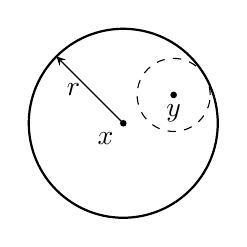
\begin{tikzpicture}[scale=0.8,>=stealth]
        \draw[thick] (0,0) circle (1.5);
        \fill (0,0) circle (1.5pt) node[below left]{$x$};
        \fill (0.8,0.45) circle (1.5pt) node[below]{$y$};
        \draw[dashed] (0.8,0.45) circle (0.58);
        \draw[->] (0,0)--(-1.06,1.06) node[midway,left]{$r$};
    \end{tikzpicture}
    \end{nscenter}
    (2) The first two claims are obvious. If $x\in U_1\cap\ldots\cap U_m$ and $B_{r_i}(x)\subset U_i$, then $B_r(x)$ with $r=\min_i r_i>0$ lies in the intersection.
\end{proof}
Infinite intersections of open sets need not be open: $\bigcap_{k}B_{1/k}(0)=\{0\}$ in $\bbR$. The minimum of infinitely many radii can be zero, and this is the only reason why finiteness is needed.

\begin{defn}[Continuity]\index{Continuous map}
    A map $f:X\to Y$ between metric spaces is \emph{continuous at} $x\in X$ if for every $\epsilon>0$ there is a $\delta>0$ such that $\rho_X(x,x')<\delta$ implies $\rho_Y(f(x),f(x'))<\epsilon$, i.e., $f(B_\delta(x))\subset B_\epsilon(f(x))$. It is \emph{continuous} if it is continuous at every point.
\end{defn}

Lipschitz maps are continuous (take $\delta=\epsilon/L$). Thus norms, distance functions and linear maps are continuous, and so are addition and multiplication of matrices, the determinant, and in general all polynomial functions of the entries.

\begin{prop}[Continuity via open sets]\label{prop continuity via open sets}
    A map $f:X\to Y$ between metric spaces is continuous iff the preimage $f^{-1}(U)$ of every open set $U\subset Y$ is open in $X$.
\end{prop}
\begin{proof}
    Suppose $f$ is continuous, $U\subset Y$ is open and $x\in f^{-1}(U)$. Some ball $B_\epsilon(f(x))$ lies in $U$, and continuity gives a ball $B_\delta(x)$ mapped into it, i.e., $B_\delta(x)\subset f^{-1}(U)$. Conversely, the preimage of the open ball $B_\epsilon(f(x))$ is open and contains $x$, hence contains some ball $B_\delta(x)$, which is exactly continuity at $x$.
\end{proof}

\begin{intu*}
    This innocent proposition is the starting point of topology. Continuity, the central notion of analysis, can be expressed without mentioning distances at all: only the collection of open sets matters. Different metrics with the same open sets have the same continuous maps. In the next \sect\ we will take the collection of open sets as the primary object and forget the metric altogether.
\end{intu*}

Convergence of sequences behaves the same way.

\begin{defn}[Convergence]\index{Limit of a sequence}\index{Convergence}
    A sequence $(x_k)$ in a metric space $X$ \emph{converges} to $x\in X$, written $x_k\to x$ or $\lim_k x_k=x$, if $\rho(x_k,x)\to0$, i.e., for every $\epsilon>0$ there is $N$ such that $\rho(x_k,x)<\epsilon$ for all $k>N$. Equivalently, every open set containing $x$ contains all but finitely many of the $x_k$.
\end{defn}

A sequence has at most one limit: if $x_k\to x$ and $x_k\to y$, then $\rho(x,y)\leq\rho(x,x_k)+\rho(x_k,y)\to0$.

\begin{prop}[Sequential continuity]\label{prop sequential continuity}
    A map $f:X\to Y$ between metric spaces is continuous at $x$ iff $x_k\to x$ implies $f(x_k)\to f(x)$ for every sequence $(x_k)$.
\end{prop}
\begin{proof}
    If $f$ is continuous at $x$ and $\epsilon>0$ is given, the $\delta$ from the definition works for all $x_k$ with $\rho(x_k,x)<\delta$, i.e., for all large $k$. Conversely, if $f$ is not continuous at $x$, then for some $\epsilon>0$ every ball $B_{1/k}(x)$ contains a point $x_k$ with $\rho_Y(f(x_k),f(x))\geq\epsilon$; then $x_k\to x$ but $f(x_k)\not\to f(x)$.
\end{proof}

Since only open sets matter for continuity and convergence, we should compare metrics by their open sets.

\begin{defn}[Equivalent metrics]\index{Metric!equivalence of}
    Two metrics $\rho_1,\rho_2$ on the same set $X$ are \emph{equivalent} if they have the same open sets. They are \emph{Lipschitz equivalent} if there are constants $c,C>0$ such that $c\,\rho_1\leq\rho_2\leq C\rho_1$.
\end{defn}

Lipschitz equivalent metrics are equivalent, because $B^{(2)}_{cr}(x)\subset B^{(1)}_r(x)$ and $B^{(1)}_{r/C}(x)\subset B^{(2)}_r(x)$, where $B^{(i)}$ denotes a ball of the metric $\rho_i$. For instance, the chordal and the angular metrics on $\bbS^n$ (Example~\ref{example sphere metrics}) are Lipschitz equivalent. The converse is false:

\begin{example}[Boundedness is not about open sets]\label{example bounded metric}
    For any metric $\rho$, the function $\rho'=\min(\rho,1)$ is again a metric. (If one of $\rho(x,y)$, $\rho(y,z)$ is at least $1$, the triangle inequality for $\rho'$ is obvious; otherwise it follows from that for $\rho$.) Balls of radius $r<1$ are the same for $\rho$ and $\rho'$, so the two metrics have the same open sets. But in the metric $\rho'$ every set is bounded, so $\rho'$ is not Lipschitz equivalent to the usual metric on $\bbR$.
\end{example}

For norms, however, the two notions of equivalence coincide: dilations turn local information into global one.

\begin{prop}[Equivalent norms]\label{prop equivalent norms}\index{Norm!equivalence of}
    Two norms $\lVert\cdot\rVert_a$ and $\lVert\cdot\rVert_b$ on a vector space $V$ define the same open sets iff there are constants $c,C>0$ such that $c\lVert v\rVert_a\leq\lVert v\rVert_b\leq C\lVert v\rVert_a$ for all $v\in V$. In this case the norms are called \emph{equivalent}.
\end{prop}
\begin{proof}
    The ``if'' direction was shown above. Conversely, the unit ball $\{\lVert v\rVert_b<1\}$ is open for $\lVert\cdot\rVert_a$, so it contains some ball $\{\lVert v\rVert_a<\delta\}$. Given $v\neq0$, the rescaled vector $w=\frac{\delta}{2}\frac{v}{\lVert v\rVert_a}$ has $\lVert w\rVert_a=\frac\delta2<\delta$, hence $\lVert w\rVert_b<1$, i.e., $\lVert v\rVert_b<\frac2\delta\lVert v\rVert_a$. The other inequality follows by symmetry.
\end{proof}

\begin{example}\label{example equivalent norms}
    \begin{enumerate}
        \item On $\bbR^n$, we have $\lVert \bf{x}\rVert_\infty\leq\lVert \bf{x}\rVert_2\leq\lVert \bf{x}\rVert_1\leq\sqrt n\lVert \bf{x}\rVert_2\leq n\lVert \bf{x}\rVert_\infty$. All inequalities are elementary except the third one, which is the Cauchy-Schwarz inequality applied to the vectors $(\lvert x^i\rvert)_i$ and $(1,\ldots,1)$. These inequalities are exactly the nesting of the balls in Figure~\ref{fig lp balls}.
        \item Applying the same inequalities to the vector of singular values, we obtain the corresponding inequalities between the matrix norms of Example~\ref{example matrix norms}:
        \[\lVert A\rVert_{\mathrm{op}}\leq\lVert A\rVert_{\mathrm{F}}\leq\lVert A\rVert_{\mathrm{tr}}\leq\sqrt n\lVert A\rVert_{\mathrm{F}}\leq n\lVert A\rVert_{\mathrm{op}}.\]
    \end{enumerate}
    We will see in Corollary~\ref{cor norms equivalent} that \emph{all} norms on a finite-dimensional vector space are equivalent. In infinite dimensions this fails dramatically.
\end{example}

\begin{example}[Inequivalent norms]\label{example tent spikes}
    On $C[0,1]$ we have $\lVert f\rVert_1\leq\lVert f\rVert_\infty$, so every set that is open for $\lVert\cdot\rVert_1$ is also open for $\lVert\cdot\rVert_\infty$. The converse fails. Consider the ``tent spikes'' $f_k(x)=\max(0,1-kx)$ (Figure~\ref{fig tent spikes}). They all have $\lVert f_k\rVert_\infty=1$, while $\lVert f_k\rVert_1=\frac{1}{2k}\to0$. Hence the ball $\{\lVert f\rVert_\infty<1\}$ is not open for $\lVert \cdot\rVert_1$: every $L^1$-ball around $0$ contains some $f_k$, which is not in it. In terms of sequences, $f_k\to 0$ in the $L^1$ norm but not uniformly. No constant $C$ can make $\lVert f\rVert_\infty\leq C\lVert f\rVert_1$ true, since a function can have a tall, thin spike of tiny area.
\end{example}

\begin{figure}[tp]
    \centering
    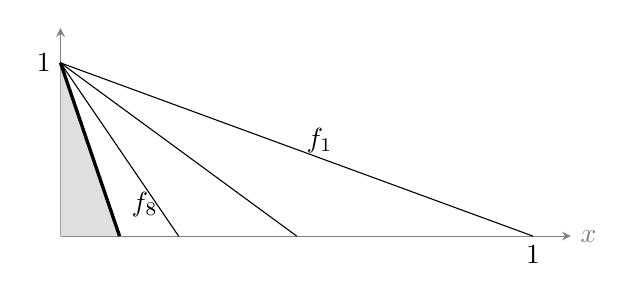
\begin{tikzpicture}[xscale=6,yscale=2.2,>=stealth]
        \draw[->,gray] (0,0)--(1.08,0) node[right]{$x$};
        \draw[->,gray] (0,0)--(0,1.2);
        \node[left] at (0,1) {$1$};
        \node[below] at (1,0) {$1$};
        \foreach \k in {1,2,4} {
            \draw (0,1)--({1/\k},0);
        }
        \fill[gray!25] (0,0)--(0,1)--(1/8,0)--cycle;
        \draw[very thick] (0,1)--(1/8,0);
        \node[right] at (0.5,0.55) {$f_1$};
        \node[right] at (0.13,0.18) {$f_8$};
    \end{tikzpicture}
    \caption{Tent spikes $f_k(x)=\max(0,1-kx)$ for $k=1,2,4,8$. Their sup norm is always $1$, while their $L^1$ norm (the shaded area for $k=8$) tends to $0$.}
    \label{fig tent spikes}
\end{figure}

\begin{xca}\label{xca angular metric}
    Prove the triangle inequality for the angular metric $\theta$ on $\bbS^n$. \emph{Hint:} let $a=\theta(\bf{x},\bf{y})$, $b=\theta(\bf{y},\bf{z})$, and write $\bf{x}=\cos a\, \bf{y}+\sin a\, \bf{u}$, $\bf{z}=\cos b\, \bf{y}+\sin b\, \bf{w}$ with unit vectors $\bf{u},\bf{w}\perp \bf{y}$. Show that $\langle \bf{x},\bf{z}\rangle\geq\cos(a+b)$.
\end{xca}
\begin{xca}\label{xca isometries of Rn}
    Show that every isometry $f$ of $\bbR^n$ (with the Euclidean metric) has the form $f(\bf{x})=A\bf{x}+\bf{b}$ with $A\in\Or_n$. \emph{Hint:} reduce to $f(0)=0$ and use the polarization identity $2\langle \bf{x},\bf{y}\rangle=\lvert \bf{x}\rvert^2+\lvert \bf{y}\rvert^2-\lvert \bf{x}-\bf{y}\rvert^2$.
\end{xca}
\begin{xca}
    Show that the operator norm is \emph{submultiplicative}, $\lVert AB\rVert_{\mathrm{op}}\leq \lVert A\rVert_{\mathrm{op}}\lVert B\rVert_{\mathrm{op}}$, and that $\lVert A\rVert_{\mathrm{op}}=\sigma_1$. Are the Frobenius and trace norms submultiplicative?
\end{xca}
\begin{xca}
    Show that the closed unit ball of the trace norm is the convex hull of the rank-one matrices $\bf{u}\bf{v}^\top$ with $\lvert \bf{u}\rvert=\lvert \bf{v}\rvert=1$. This is the matrix analog of the fact that the diamond in Figure~\ref{fig lp balls} is the convex hull of the points $\pm \bf{e}_i$.
\end{xca}
\begin{xca}
    Show that $\rho/(1+\rho)$ is a metric whenever $\rho$ is, and that it has the same open sets as $\rho$.
\end{xca}
\begin{xca}
    Show that on the space of sequences with finitely many nonzero terms, the norms $\lVert\cdot\rVert_1$ and $\lVert\cdot\rVert_\infty$ are not equivalent.
\end{xca}


\section{Topological spaces}\label{sec: topological spaces}

Proposition~\ref{prop metric open sets} lists the basic properties of the open sets of a metric space, and Proposition~\ref{prop continuity via open sets} shows that continuity depends only on these open sets. Let us take these properties as axioms.

\begin{defn}[Topology]\index{Topological space}\index{Topology}
    A \emph{topology} on a set $X$ is a collection $\mathcal{T}$ of subsets of $X$ such that
    \begin{enumerate}
        \item $\varnothing, X\in\mathcal{T}$;
        \item $\mathcal{T}$ is closed under arbitrary (finite or infinite) unions;
        \item $\mathcal{T}$ is closed under finite intersections.
    \end{enumerate}
    The elements of $\mathcal{T}$ are called \emph{open sets}, and the pair $(X,\mathcal{T})$ is called a \emph{topological space}. Usually we will just write $X$ when the topology is clear from the context.
\end{defn}

\begin{example}\label{example topologies}
    \begin{enumerate}
        \item \emph{Metric topology.}\index{Topology!metric} The open sets of a metric space form a topology. A topological space is called \emph{metrizable}\index{Metrizable space} if its topology comes from some metric. By definition, equivalent metrics define the same topology. Thus $\bbR^n$ with any of the norms of Example~\ref{example lp norms} has one and the same \emph{standard topology}, and so does $\bbS^n$ with the chordal or the angular metric. Unless explicitly stated otherwise, $\bbR^n$, $\bbC^n$, $\bbS^n$, $\Mat_n(\bbR)\cong\bbR^{n^2}$, and their subsets carry these standard topologies.
        \item \emph{Discrete topology.}\index{Topology!discrete} All subsets of $X$ are open. This is the metric topology of the discrete metric: the space ``falls apart'' into separate points.
        \item \emph{Trivial topology.}\index{Topology!trivial} Only $\varnothing$ and $X$ are open. Such a space cannot distinguish any of its points from each other. If $X$ has at least two points, this topology is not metrizable, because in a metric space the ball of radius $\rho(x,y)$ around $x$ is an open set containing $x$ but not $y$.
        \item \emph{Sierpi\'nski space.}\index{Sierpi\'nski space} On the two-point set $\mathsf{S}=\{0,1\}$ take the open sets $\varnothing,\{1\},\{0,1\}$. Here $1$ has an open neighborhood not containing $0$, but not vice versa. This asymmetry is impossible in a metric space, so $\mathsf{S}$ is not metrizable. Such spaces will be excluded in almost all of our applications (see \S\ref{Separation Axioms}), but $\mathsf{S}$ is a useful bookkeeping device, see Exercise~\ref{xca Sierpinski}.
    \end{enumerate}
\end{example}

\begin{intu*}
    An open set is a set that, together with each of its points, contains ``all points sufficiently close to it''. The topology encodes this notion of closeness without any numbers: the smaller the open sets containing two points, the ``closer'' these points are. In a metric space, \emph{every} open set containing $x$ contains a whole ball $B_r(x)$, which is exactly the formalization of ``all points close enough to $x$''. Topology retains only this qualitative information.
\end{intu*}

\begin{defn}[Neighborhood]\index{Neighborhood}
    A set $N\subset X$ is a \emph{neighborhood} of a point $x\in X$ if it contains an open set $U$ with $x\in U$. If $N$ itself is open, it is called an \emph{open neighborhood} of $x$.
\end{defn}

\begin{prop}[Open iff a neighborhood of each point]\label{open iff contains neighborhoods}
    A set $M\subset X$ is open iff it is a neighborhood of each of its points, i.e., for every $x\in M$ there is an open set $U_x$ with $x\in U_x\subset M$.
\end{prop}
\begin{proof}
    If the condition holds, then $M=\bigcup_{x\in M}U_x$ is a union of open sets.
\end{proof}

\begin{defn}[Closed set]\index{Closed set}\index{Clopen set}
    A set $A\subset X$ is \emph{closed} if its complement $X\setminus A$ is open. A set that is both closed and open is called \emph{clopen}.
\end{defn}

\begin{prop}\label{prop closed sets}
    In a topological space $X$, the sets $\varnothing$ and $X$ are closed (in fact clopen), arbitrary intersections of closed sets are closed, and finite unions of closed sets are closed.
\end{prop}
\begin{proof}
    Take complements in the definition of a topology, using $X\setminus\bigcup_\alpha U_\alpha=\bigcap_\alpha(X\setminus U_\alpha)$.
\end{proof}

A topology can therefore be equivalently described by the collection of its closed sets. Note that ``closed'' is not the opposite of ``open'': the half-open interval $[0,1)\subset\bbR$ is neither, while in a discrete space every set is both.

\begin{example}
    In a metric space, closed balls $\wb{B}_r(x)$ are closed: if $\rho(x,y)>r$, then the ball $B_{\rho(x,y)-r}(y)$ does not meet $\wb{B}_r(x)$ by the triangle inequality. In particular, points are closed, and so are all finite sets. The integers $\bbZ\subset\bbR$ form a closed set, and so does the sphere $\bbS^n\subset\bbR^{n+1}$.
\end{example}

\begin{defn}[Interior, closure, boundary]\index{Interior}\index{Closure}\index{Boundary of a subset}
    Let $A\subset X$.
    \begin{enumerate}
        \item The \emph{interior} $\Int A$ is the union of all open sets contained in $A$; it is the largest open subset of $A$.
        \item The \emph{closure} $\wb{A}$ is the intersection of all closed sets containing $A$; it is the smallest closed set containing $A$.
        \item The \emph{boundary} is $\partial A=\wb{A}\setminus\Int A$.
    \end{enumerate}
\end{defn}

We have $\Int A\subset A\subset\wb{A}$, and taking complements interchanges interior and closure: $X\setminus\wb{A}=\Int(X\setminus A)$. Hence also $\partial A=\wb{A}\cap\wb{X\setminus A}$, so a set and its complement have the same boundary (Figure~\ref{fig int closure boundary}).

\begin{figure}[tp]
    \centering
    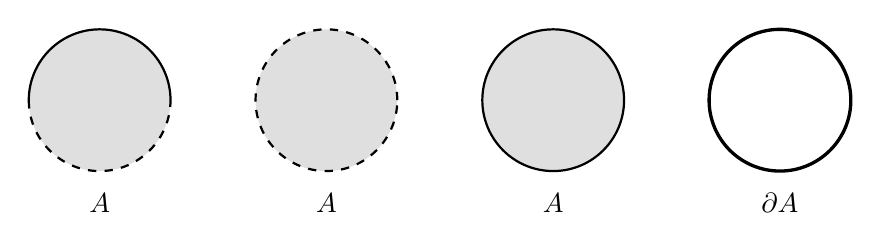
\begin{tikzpicture}[scale=0.9,>=stealth]
        \begin{scope}
            \fill[gray!25] (0,0) circle (1);
            \draw[thick] (1,0) arc (0:180:1);
            \draw[thick,dashed] (-1,0) arc (180:360:1);
            \node at (0,-1.45) {$A$};
        \end{scope}
        \begin{scope}[shift={(3.2,0)}]
            \fill[gray!25] (0,0) circle (1);
            \draw[thick,dashed] (0,0) circle (1);
            \node at (0,-1.45) {$\Int A$};
        \end{scope}
        \begin{scope}[shift={(6.4,0)}]
            \fill[gray!25] (0,0) circle (1);
            \draw[thick] (0,0) circle (1);
            \node at (0,-1.45) {$\wb{A}$};
        \end{scope}
        \begin{scope}[shift={(9.6,0)}]
            \draw[very thick] (0,0) circle (1);
            \node at (0,-1.45) {$\partial A$};
        \end{scope}
    \end{tikzpicture}
    \caption{A disk $A\subset\bbR^2$ containing the upper half of its boundary circle (solid lines belong to the set, dashed ones do not), together with its interior, closure and boundary.}
    \label{fig int closure boundary}
\end{figure}

\begin{prop}[Points of the closure]\label{prop closure}
    \begin{enumerate}
        \item A point $x$ lies in $\wb{A}$ iff every neighborhood of $x$ meets $A$.
        \item If $X$ is a metric space, then $x\in\wb{A}$ iff $x=\lim_k a_k$ for some sequence $(a_k)$ in $A$.
    \end{enumerate}
\end{prop}
\begin{proof}
    (1) We have $x\notin\wb{A}$ iff there is a closed $F\supset A$ with $x\notin F$, iff the open set $U=X\setminus F$ is a neighborhood of $x$ disjoint from $A$.

    (2) If $x\in\wb{A}$, pick $a_k\in A\cap B_{1/k}(x)$ using (1); then $a_k\to x$. Conversely, if $a_k\to x$, every ball around $x$ contains some $a_k$, so $x\in\wb{A}$ by (1).
\end{proof}

\begin{defn}[Limit points]\index{Limit point}\index{Isolated point}
    A point $x\in X$ is a \emph{limit point} (or \emph{accumulation point}) of $A\subset X$ if every neighborhood of $x$ meets $A$ in a point other than $x$. A point of $A$ that is not a limit point of $A$ is called \emph{isolated}.
\end{defn}

By Proposition~\ref{prop closure}, $\wb{A}$ is the union of $A$ and its limit points. Note that a point of $A$ need not be a limit point of $A$: in $A=\{0\}\cup(1,2)\subset\bbR$, the point $0$ is isolated, while the limit points of $A$ form the interval $[1,2]$. The set $\bbZ\subset\bbR$ has no limit points at all.

\begin{example}\label{example closure of ball}
    In a normed space, the closure of the open ball $B_r(x)$ is the closed ball $\wb{B}_r(x)$, and the boundary of either is the sphere $\{y\mid\lVert y-x\rVert=r\}$ (Exercise~\ref{xca closure of ball}). In general metric spaces this fails: for the discrete metric, $B_1(x)=\{x\}$ is already closed, while $\wb{B}_1(x)=X$. Thus our notation $\wb{B}_r(x)$ for the closed ball is a definition and not a statement about closures.
\end{example}

\begin{defn}[Dense subset]\index{Dense subset}
    A subset $A\subset X$ is \emph{dense} if $\wb{A}=X$, i.e., if every nonempty open set meets $A$.
\end{defn}

For example, $\bbQ^n$ is dense in $\bbR^n$, while $\Int\bbQ=\varnothing$ and $\partial\bbQ=\bbR$ in $\bbR$. Invertible matrices are dense in $\Mat_n(\bbR)$, because $\det(A+t\cdot\rmI_n)$ is a nonzero polynomial in $t$ and therefore vanishes only for finitely many $t$.

\subsection{Bases and countability}

Most topologies are described not by listing all open sets but by specifying enough of them, as we did with balls in metric spaces.

\begin{defn}[Basis]\index{Basis of topology}
    A collection $\mathfrak{B}\subset\mathcal{T}$ of open sets is a \emph{basis} of the topology $\mathcal{T}$ if every open set is a union of elements of $\mathfrak{B}$.
\end{defn}

\begin{prop}\label{characterization of topology using basis}
    A collection $\mathfrak{B}\subset\mathcal{T}$ is a basis of $\mathcal{T}$ iff for every open set $U$ and every $x\in U$ there is a $B\in\mathfrak{B}$ with $x\in B\subset U$.
\end{prop}
\begin{proof}
    If the condition holds, $U$ is the union of these $B$'s. The converse is clear.
\end{proof}

Conversely, we may start with a collection of subsets and ask which topology it generates.

\begin{prop}[Generating a topology]\label{prop generating topology}\index{Topology!generated by a family of sets}
    Let $\mathfrak{B}$ be a collection of subsets of a set $X$. The unions of elements of $\mathfrak{B}$ form a topology (with basis $\mathfrak{B}$) iff
    \begin{enumerate}
        \item $\mathfrak{B}$ covers $X$, i.e., $\bigcup_{B\in\mathfrak{B}}B=X$, and
        \item for every $x\in B_1\cap B_2$ with $B_1,B_2\in\mathfrak{B}$ there is a $B_3\in\mathfrak{B}$ with $x\in B_3\subset B_1\cap B_2$.
    \end{enumerate}
    More generally, for any collection $\mathfrak{S}$ of subsets of $X$, the finite intersections of elements of $\mathfrak{S}$ (including $X$ itself as the empty intersection) satisfy these conditions. The resulting topology is the coarsest one in which all elements of $\mathfrak{S}$ are open; it is called the topology \emph{generated} by $\mathfrak{S}$, and $\mathfrak{S}$ is called its \emph{subbasis}\index{Subbasis of topology}.
\end{prop}
\begin{proof}
    Unions of unions are unions, so the only issue is intersections. Condition (2) says exactly that $B_1\cap B_2$ is a union of elements of $\mathfrak{B}$, and then so is the intersection of any two unions of elements of $\mathfrak{B}$. Condition (1) says that $X$ is such a union. The last claim is clear.
\end{proof}

\begin{example}\label{examples of basis of topology}
    \begin{enumerate}
        \item The open balls form a basis of the metric topology. In $\bbR^n$ it is enough to take the balls $B_r(x)$ with rational radii $r$ and rational centers $\bf{x}\in\bbQ^n$, a \emph{countable} basis.
        \item One-point sets form a basis of the discrete topology.
        \item Open intervals form a basis of the standard topology on $\bbR$. In fact, every open set in $\bbR$ is a disjoint union of at most countably many open intervals, possibly unbounded (Exercise~\ref{xca open sets in R}).
    \end{enumerate}
\end{example}

\begin{defn}[Countability axioms]\index{Second countable space}\index{Separable space}
    A topological space is \emph{second countable} if its topology has a countable basis, and \emph{separable}\index{Countability axioms} if it has a countable dense subset.
\end{defn}

\begin{prop}\label{prop second countable separable}
    \begin{enumerate}
        \item Every second countable space is separable.
        \item Every separable metric space is second countable.
    \end{enumerate}
\end{prop}
\begin{proof}
    (1) Pick one point in each nonempty element of a countable basis. Every nonempty open set contains a basis element, hence one of these points.

    (2) Let $D$ be a countable dense subset. We claim that the countably many balls $B_{1/m}(d)$, $d\in D$, $m\in\bbN$, form a basis. Given an open $U$ and $x\in U$, choose $r$ with $B_r(x)\subset U$, then $m$ with $2/m<r$, and $d\in D$ with $\rho(x,d)<1/m$. Then $x\in B_{1/m}(d)\subset B_r(x)\subset U$.
\end{proof}

Second countability is a mild smallness condition, and almost all spaces in this book will have it. Infinite-dimensional spaces, however, may fail it.

\begin{example}[Separable and non-separable sequence spaces]\label{example separability}
    \begin{enumerate}
        \item The space $\ell^\infty$ is \emph{not} separable. For every subset $S\subset\bbN$, consider its indicator sequence $\chi_S$ (with $1$ at the positions in $S$ and $0$ elsewhere). There are uncountably many of them, and any two are at distance exactly $1$. The balls of radius $\frac12$ around them are therefore disjoint, and a dense subset must meet each of them.
        \item The spaces $c_0$ and $\ell^p$, $1\leq p<\infty$, are separable: sequences with finitely many nonzero terms, all rational, are dense, because the tails of every element of these spaces are small.
        \item The space $C[0,1]$ with the sup norm is separable: piecewise-linear functions with rational break points and rational values are dense. Indeed, every continuous function on $[0,1]$ is uniformly continuous (Proposition~\ref{prop uniform continuity}), so it is uniformly close to its piecewise-linear interpolation on a fine enough rational grid.
    \end{enumerate}
\end{example}

\subsection{Continuous maps}

\begin{defn}[Continuous map]\index{Continuous map}
    A map $f:X\to Y$ between topological spaces is \emph{continuous} if the preimage $f^{-1}(U)$ of every open set $U\subset Y$ is open in $X$. It is \emph{continuous at} $x\in X$ if for every neighborhood $V$ of $f(x)$ there is a neighborhood $U$ of $x$ with $f(U)\subset V$. The set of all continuous maps $X\to Y$ is denoted $C(X,Y)$.
\end{defn}

By Proposition~\ref{prop continuity via open sets}, for metric spaces this agrees with the $\epsilon$-$\delta$ definition. Equivalently, $f$ is continuous iff preimages of closed sets are closed, since $f^{-1}(Y\setminus A)=X\setminus f^{-1}(A)$. By Proposition~\ref{open iff contains neighborhoods}, $f$ is continuous iff it is continuous at every point. It is also enough to check that preimages of the elements of a basis (or even a subbasis) of $Y$ are open, since preimages commute with unions and intersections.

Compositions of continuous maps are obviously continuous, and so are identity maps. Thus we have the category $\mathsf{Top}$\index{Category!of topological spaces} of topological spaces and continuous maps, together with the forgetful functor $\mathsf{Top}\to\mathsf{Set}$. Every map from a discrete space and every map into a trivial space is continuous.

\begin{example}[Zero sets]\label{example zero sets}
    If $f:X\to\bbR^m$ is continuous, its \emph{zero set}\index{Zero set}\index{General linear group}\index{Orthogonal group}\index{Special linear group} $f^{-1}(0)$ is closed and the set $\{f\neq 0\}$ is open. Since polynomials in matrix entries are continuous, the sets
    \[\Or_n=\{A\mid A^\top A=\rmI_n\},\qquad \SL_n(\bbR)=\{A\mid\det A=1\}\]
    are closed in $\Mat_n(\bbR)$, while $\GL_n(\bbR)=\{A\mid\det A\neq0\}$ is open and, as we saw above, dense.
\end{example}

\begin{prop}[Dense sets determine maps]\label{prop dense determines maps}
    Let $f,g:X\to Y$ be continuous maps into a metric space, and suppose $f=g$ on a dense subset $D\subset X$. Then $f=g$.
\end{prop}
\begin{proof}
    Suppose $f(x)\neq g(x)$, let $\epsilon=\frac12\rho(f(x),g(x))$, and consider the open set
    \[U=f^{-1}(B_\epsilon(f(x)))\cap g^{-1}(B_\epsilon(g(x))).\]
    It contains $x$, and $f\neq g$ everywhere on $U$ because the two balls are disjoint. But $U$ must meet $D$.
\end{proof}
This is the reason why the inclusion $\bbQ\hookrightarrow\bbR$ is an epimorphism in the category of metrizable topological rings, even though it is not surjective (see \S\ref{sec: classes of morphisms}; we will extend this to all Hausdorff topological rings in Proposition~\ref{prop Hausdorff diagonal}).

\begin{defn}[Homeomorphism]\index{Homeomorphism}
    A \emph{homeomorphism} is a continuous bijection whose inverse is also continuous, i.e., an isomorphism in the category $\mathsf{Top}$. Spaces $X$ and $Y$ are \emph{homeomorphic}, $X\cong Y$, if there is a homeomorphism between them.
\end{defn}

\begin{example}\label{example homeomorphisms}
    \begin{enumerate}
        \item The open ball $B_1(0)\subset\bbR^n$ is homeomorphic to $\bbR^n$ via $\bf{x}\mapsto\frac{\bf{x}}{1-\lvert \bf{x}\rvert}$, with inverse $\bf{y}\mapsto\frac{\bf{y}}{1+\lvert \bf{y}\rvert}$. In particular, $(-1,1)\cong\bbR$. Size is not a topological notion.
        \item The unit balls of any two norms on $\bbR^n$ are homeomorphic. For instance, the square $\{\lVert \bf{x}\rVert_\infty\leq 1\}$ is mapped onto the round disk $\{\lVert \bf{x}\rVert_2\leq1\}$ by the radial rescaling $\bf{x}\mapsto\frac{\lVert \bf{x}\rVert_\infty}{\lVert \bf{x}\rVert_2}\bf{x}$ (and $0\mapsto0$), whose inverse is $\bf{x}\mapsto\frac{\lVert \bf{x}\rVert_2}{\lVert \bf{x}\rVert_\infty}\bf{x}$. Both maps are continuous away from $0$, and also at $0$, because the ratio of the two norms is bounded (Example~\ref{example equivalent norms}). Corners are not a topological notion either.
        \item \emph{Stereographic projection.}\index{Stereographic projection} Let $N=(0,\ldots,0,1)$ be the north pole of $\bbS^n\subset\bbR^{n+1}$. Projecting from $N$ onto the equatorial plane $\bbR^n=\{x^{n+1}=0\}$ (Figure~\ref{fig stereographic}) gives a homeomorphism
        \[\varphi_N:\bbS^n\setminus\{N\}\to\bbR^n,\quad \varphi_N(\bf{x})=\frac{(x^1,\ldots,x^n)}{1-x^{n+1}},\qquad \varphi_N^{-1}(\bf{y})=\frac{(2\bf{y},\;\lvert \bf{y}\rvert^2-1)}{\lvert \bf{y}\rvert^2+1}.\]
        Points close to $N$ are sent far away, so the sphere is the plane with ``one point added at infinity''.
        \item If $f:\bbR^n\to\bbR^m$ is continuous, then its graph $\Gamma_f=\{(\bf{x},f(\bf{x}))\}\subset\bbR^{n+m}$ is homeomorphic to $\bbR^n$: the projection $(\bf{x},\bf{y})\mapsto \bf{x}$ is continuous, and so is its inverse $\bf{x}\mapsto(\bf{x},f(\bf{x}))$.
    \end{enumerate}
\end{example}

\begin{figure}[tp]
    \centering
    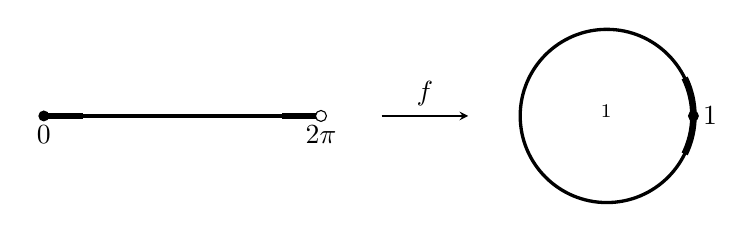
\begin{tikzpicture}[scale=1.1,>=stealth]
        \draw[very thick] (0,0)--(3.2,0);
        \draw[line width=2.4pt] (0,0)--(0.45,0) (2.75,0)--(3.2,0);
        \fill (0,0) circle (1.8pt) node[below]{$0$};
        \draw[fill=white] (3.2,0) circle (1.8pt) node[below]{$2\pi$};
        \draw[->] (3.9,0)--(4.9,0) node[midway,above]{$f$};
        \draw[very thick] (6.5,0) circle (1);
        \draw[line width=2.4pt] (7.5,0) arc (0:26:1) (7.5,0) arc (0:-26:1);
        \fill (7.5,0) circle (1.8pt) node[right]{$1$};
        \node at (6.5,0) {$\bbS^1$};
    \end{tikzpicture}
    \caption{The map $f(t)=\rme^{\rmi t}$. A neighborhood of $1$ in the circle (heavy arc) has a preimage consisting of two pieces at opposite ends of the interval.}
    \label{fig bijection not homeo}
\end{figure}

\begin{figure}[tp]
    \centering
    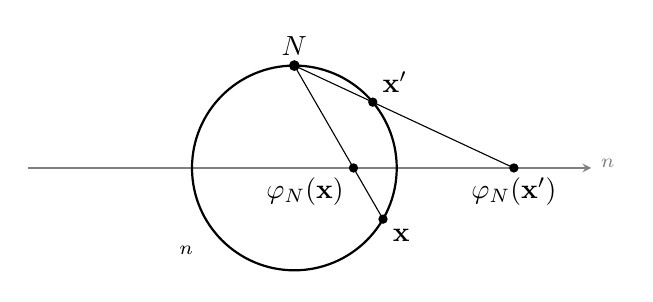
\begin{tikzpicture}[scale=1.3,>=stealth]
        \draw[->,gray] (-2.6,0)--(2.9,0) node[right]{$\bbR^n$};
        \draw[thick] (0,0) circle (1);
        \fill (0,1) circle (1.5pt) node[above]{$N$};
        % lower point
        \fill ({cos(-30)},{sin(-30)}) circle (1.3pt) node[below right]{$\bf{x}$};
        \draw (0,1)--({cos(-30)},{sin(-30)});
        \fill (0.5774,0) circle (1.3pt) node[below left]{$\varphi_N(\bf{x})$};
        % upper point
        \fill ({cos(40)},{sin(40)}) circle (1.3pt) node[above right]{$\bf{x}'$};
        \draw (0,1)--(2.1445,0);
        \fill (2.1445,0) circle (1.3pt) node[below]{$\varphi_N(\bf{x}')$};
        \node at (-1.05,-0.85) {$\bbS^n$};
    \end{tikzpicture}
    \caption{Stereographic projection from the north pole $N$. Points close to $N$ are sent far away from the origin.}
    \label{fig stereographic}
\end{figure}

\begin{example}[A continuous bijection that is not a homeomorphism]\label{example bijection not homeo}
    The map $f:[0,2\pi)\to\bbS^1$, $f(t)=\rme^{\rmi t}$, is a continuous bijection, but its inverse is not continuous at $1\in\bbS^1$: points $\rme^{-\rmi\epsilon}$ just below $1$ are sent to $2\pi-\epsilon$, far away from $f^{-1}(1)=0$. The interval has been ``closed up'' into a circle, and no continuous inverse can tear it open again. In categorical terms (\S\ref{sec: classes of morphisms}), $f$ is a bimorphism in $\mathsf{Top}$ (it is injective and surjective), yet it is not an isomorphism (Figure~\ref{fig bijection not homeo}).
\end{example}

Properties of topological spaces that are preserved by homeomorphisms are called \emph{topological invariants}\index{Topological invariant}. Topological invariants can take values in words (``connected''/``disconnected'', ``compact''/``non-compact''), in integers (winding numbers, Euler characteristic, genus, etc.), in groups (homotopy groups, homology groups, etc.), and in more complicated classes of objects. Some of them, like the number of path-connected components or the fundamental group, are invariant under the much weaker relation of homotopy equivalence (\S\ref{sec.homotopy}), while others, like compactness, are not. The only way to show that two spaces are \emph{not} homeomorphic is to find a topological invariant that distinguishes them.
\begin{gather*}
    \boxed{\begin{array}{c}
    \text{The problem topology serves to solve is:}\\
    \text{Are two given topological spaces homeomorphic/homotopy equivalent or not?}\\
    \text{If not, what \emph{topological invariant} distinguishes them?}
    \end{array}}
\end{gather*}
Since there is no universal algorithm that answers the first question, most of the hard work in topology goes into constructing new topological invariants and computing them. The part of topology that is especially efficient at finding such invariants is \emph{algebraic topology}, which is the subject of \Part~\ref{Part Homology}.

\begin{rem}
    In some applications, like knot theory, we are interested in \emph{ambient isotopies}\index{Ambient isotopy}: two subspaces $K,K'\subset Z$ are ambient isotopic if there is a continuous family $h_t$ of homeomorphisms of the ambient space $Z$, starting at $h_0=\id_Z$, with $h_1(K)=K'$. This is a much more restrictive relation than homeomorphism, which allows for more refined invariants like knot polynomials. These would not be invariant under homeomorphisms: every knot, as a space by itself, is just a circle! In particular, there are more chances to find a complete system of ambient isotopy invariants for certain classes of embeddings, therefore completely classifying all such objects by a fixed set of invariants.

    Beyond ambient isotopy, there are many other kinds of topological isomorphisms on various categories of topological spaces, but the basic task of topology remains the same: identify invariants that help classify spaces up to isomorphism.
\end{rem}

Finally, a set can carry many topologies, and they can be compared.

\begin{defn}[Comparison of topologies]\index{Topology!fine}\index{Topology!coarse}
    Let $\tau,\sigma$ be two topologies on a set $X$. If $\tau\subset\sigma$, we say that $\sigma$ is \emph{finer} than $\tau$, and $\tau$ is \emph{coarser} than $\sigma$.
\end{defn}

Equivalently, $\sigma$ is finer than $\tau$ iff the identity map $(X,\sigma)\to(X,\tau)$ is continuous. The trivial topology is the coarsest and the discrete topology is the finest. A finer topology on the source admits more continuous maps out of it, and a coarser topology on the target admits more continuous maps into it: $C((X,\tau),Y)\subset C((X,\sigma),Y)$ and $C(Y,(X,\sigma))\subset C(Y,(X,\tau))$. For instance, by Example~\ref{example tent spikes}, the sup-norm topology on $C[0,1]$ is strictly finer than the $L^1$ topology.

\begin{xca}\label{xca open sets in R}
    Show that every open subset of $\bbR$ is a disjoint union of at most countably many open intervals. \emph{Hint:} for $x\in U$, take the largest open interval containing $x$ and contained in $U$; each such interval contains a rational number.
\end{xca}
\begin{xca}\label{xca closure of ball}
    Prove the claims of Example~\ref{example closure of ball} about balls in normed spaces.
\end{xca}
\begin{xca}
    Show that $\wb{A\cup B}=\wb{A}\cup\wb{B}$ and $\Int(A\cap B)=\Int A\cap\Int B$, but that $\Int(A\cup B)$ can be strictly larger than $\Int A\cup\Int B$.
\end{xca}
\begin{xca}
    Show that a map $f:X\to Y$ is continuous iff $f(\wb{A})\subset\wb{f(A)}$ for every $A\subset X$.
\end{xca}
\begin{xca}\label{xca dense in circle}
    \begin{enumerate}
        \item Show that $\wb{\bbQ}=\bbR$.
        \item Show that the set $\{\rme^{2\pi\rmi \alpha n}\}_{n\in\bbZ}$ is dense in the unit circle $\bbS^1\subset \bbC$ if and only if $\alpha$ is irrational. \emph{Hint:} two of the points $\rme^{2\pi\rmi\alpha n}$, $n=0,\ldots,N$, are at distance less than $2\pi/N$, so some power of $\rme^{2\pi\rmi\alpha}$ is a rotation by a small nonzero angle.
    \end{enumerate}
\end{xca}
\begin{xca}\label{xca Sierpinski}
    Show that continuous maps $X\to\mathsf{S}$ into the Sierpi\'nski space are in natural bijection with open subsets of $X$. In the language of Example~\ref{hom-functor example}, the contravariant functor $\mathsf{Top}\to\mathsf{Set}$ sending $X$ to its topology is represented by $\mathsf{S}$.
\end{xca}


\section{Constructing spaces}\label{sec: constructing spaces}

Most interesting spaces are built from simpler ones: by taking subsets, products, and especially by gluing. In each case the underlying set is the obvious one, and the only question is which topology to put on it. There is a single principle that answers this question in all cases at once: choose the topology that makes the relevant maps continuous and is \emph{universal} with this property, in the sense of \S\ref{Sec.Products}.

\begin{defn}[Initial and final topologies]\index{Topology!initial}\index{Topology!final}
    \begin{enumerate}
        \item Let $X$ be a set and $f_i:X\to Y_i$ a family of maps into topological spaces. The \emph{initial topology} on $X$ is the coarsest topology for which all $f_i$ are continuous, i.e., the topology generated by the sets $f_i^{-1}(U)$ with $U\subset Y_i$ open.
        \item Let $Y$ be a set and $f_i:X_i\to Y$ a family of maps from topological spaces. The \emph{final topology} on $Y$ is the finest topology for which all $f_i$ are continuous: $U\subset Y$ is open iff $f_i^{-1}(U)$ is open for all $i$.
    \end{enumerate}
\end{defn}

\begin{prop}[Universal properties]\label{prop initial final universal}\index{Universal property!of initial and final topologies}
    \begin{enumerate}
        \item If $X$ carries the initial topology for $f_i:X\to Y_i$, then a map $g:Z\to X$ from any space $Z$ is continuous iff all composites $f_i\circ g$ are continuous.
        \item If $Y$ carries the final topology for $f_i:X_i\to Y$, then a map $g:Y\to Z$ into any space $Z$ is continuous iff all composites $g\circ f_i$ are continuous.
    \end{enumerate}
\end{prop}
\begin{proof}
    (1) If all $f_i\circ g$ are continuous, then the preimages $g^{-1}(f_i^{-1}(U))=(f_i\circ g)^{-1}(U)$ of the subbasic open sets are open. (2) If all $g\circ f_i$ are continuous and $V\subset Z$ is open, then $f_i^{-1}(g^{-1}(V))$ is open for all $i$, which is exactly the definition of $g^{-1}(V)$ being open in the final topology. The ``only if'' parts are clear.
\end{proof}

\begin{intu*}
    Maps \emph{into} a space with an initial topology are tested by composing with the $f_i$; maps \emph{out of} a space with a final topology are tested by precomposing with the $f_i$. This is all one ever needs to know about these topologies, and it determines them uniquely: the identity map between two topologies on $X$ with the same universal property is continuous in both directions. All constructions below are special cases.
\end{intu*}

\subsection{Subspaces and embeddings}

\begin{defn}[Subspace topology]\index{Subspace topology}\index{Embedding}
    The \emph{subspace topology} on $A\subset X$ is the initial topology for the inclusion $A\hookrightarrow X$; its open sets are the intersections $A\cap U$ with $U\subset X$ open. A continuous injective map $f:Y\to X$ is an \emph{embedding}\index{Embedding!topological} if it is a homeomorphism onto its image $f(Y)$ with the subspace topology.
\end{defn}

For a subset of a metric space, the subspace topology is the metric topology of the restricted metric, since $B^A_r(a)=A\cap B_r(a)$. By Proposition~\ref{prop initial final universal}, a map into $A$ is continuous iff it is continuous as a map into $X$. Note that open (or closed) subsets of $A$ need not be open (or closed) in $X$: the interval $(0,1]$ is closed in the subspace $(0,2)\subset\bbR$ but not in $\bbR$.

\begin{example}
    The sphere $\bbS^n$, the orthogonal group $\Or_n$, and the special linear group $\SL_n(\bbR)$ are subspaces of $\bbR^{n+1}$ and $\Mat_n(\bbR)$. The inclusion of the equator $\bbS^{n-1}\hookrightarrow\bbS^n$, $\bf{x}\mapsto(\bf{x},0)$, and the graph map $\bf{x}\mapsto(\bf{x},f(\bf{x}))$ of a continuous function (Example~\ref{example homeomorphisms}) are embeddings.
\end{example}

Continuous injective maps can fail to be embeddings for the same reason as in Example~\ref{example bijection not homeo}.

\begin{example}[Injective maps that are not embeddings]\label{example not embeddings}
    \begin{enumerate}
        \item The map $\beta:(-\pi,\pi)\to\bbR^2$, $\beta(t)=(\sin 2t,\sin t)$, is a continuous injection whose image is a figure eight (Figure~\ref{fig figure eight}). As $t\to\pm\pi$, the curve returns to the origin $\beta(0)$. So points of the image close to the origin may have preimages close to $\pm\pi$, far away from $0$, and $\beta^{-1}$ is not continuous at the origin.
        \item Let $\alpha$ be irrational and consider $\gamma:\bbR\to\bbS^1\times\bbS^1\subset\bbC^2$, $\gamma(t)=(\rme^{2\pi\rmi t},\rme^{2\pi\rmi\alpha t})$, a line of irrational slope wound around the torus. It is injective, but the points $\gamma(n)=(1,\rme^{2\pi\rmi\alpha n})$, $n\in\bbZ$, come arbitrarily close to $\gamma(0)$ (Exercise~\ref{xca dense in circle}), so again $\gamma^{-1}$ is not continuous. By the same exercise, the image of $\gamma$ is even dense in the torus.
    \end{enumerate}
\end{example}

\begin{figure}[tp]
    \centering
    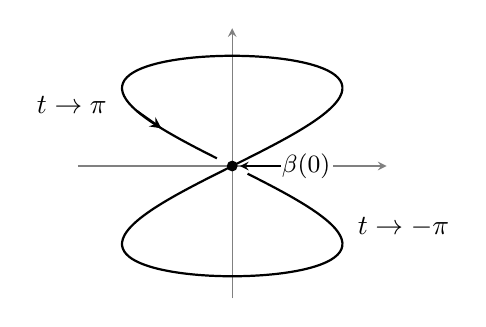
\begin{tikzpicture}[scale=1.4,>=stealth]
        \draw[->,gray] (-1.4,0)--(1.4,0);
        \draw[->,gray] (0,-1.2)--(0,1.25);
        \draw[thick,domain=-176:176,samples=150,smooth,variable=\t] plot ({sin(2*\t)},{sin(\t)});
        \fill (0,0) circle (1.4pt);
        \node[right,fill=white,inner sep=1pt] at (0.42,0) {\small $\beta(0)$};
        \draw[->,shorten >=2pt] (0.44,0)--(0.02,0);
        \draw[->,thick] ({sin(2*150)},{sin(150)}) -- ({sin(2*160)},{sin(160)});
        \node[left] at (-1.05,0.55) {$t\to\pi$};
        \node[right] at (1.05,-0.55) {$t\to-\pi$};
    \end{tikzpicture}
    \caption{The injective curve $\beta(t)=(\sin2t,\sin t)$, $t\in(-\pi,\pi)$. Its ends approach the point $\beta(0)$, so $\beta$ is not an embedding.}
    \label{fig figure eight}\label{fig:immersion}
\end{figure}

\subsection{Products and sums}

\begin{defn}[Product topology]\index{Product (in topology)}
    The \emph{product topology}\index{Topology!product} on $X=\prod_{i\in I}X_i$ is the initial topology for the projections $\pr_i:X\to X_i$. A basis is given by the products $\prod_i U_i$ of open sets $U_i\subset X_i$ such that $U_i=X_i$ for all but finitely many $i$.
\end{defn}

By Proposition~\ref{prop initial final universal}, a map $g=(g_i):Z\to\prod_iX_i$ is continuous iff all its components $g_i=\pr_i\circ g$ are. This is precisely the statement that $\prod_iX_i$ is the categorical product in $\mathsf{Top}$ (\S\ref{Sec.Products}).

\begin{example}\label{example products}
    \begin{enumerate}
        \item For metric spaces $X_1,\ldots,X_n$, the product topology on $X_1\times\cdots\times X_n$ is the metric topology of $\rho((x_i),(y_i))=\max_i\rho_i(x_i,y_i)$, whose balls are products of balls. In particular, the standard topology on $\bbR^n$ is the product topology of $n$ copies of $\bbR$, and $\Mat_n(\bbR)\cong\bbR^{n^2}$.
        \item The $n$-\emph{torus}\index{Torus} $\bbT^n=\bbS^1\times\cdots\times\bbS^1\subset\bbC^n$. More generally, products of spheres such as $\bbS^2\times\bbS^1$ are among the simplest spaces we can construct.
        \item \emph{Pointwise convergence.}\index{Convergence!pointwise} The set $\bbR^X=\prod_{x\in X}\bbR$ of all functions $f:X\to\bbR$ on a set $X$ carries the product topology. A sequence $f_k$ converges to $f$ in it iff $f_k(x)\to f(x)$ for every $x\in X$: every basic neighborhood of $f$ constrains only finitely many values $f(x_1),\ldots,f(x_m)$.
    \end{enumerate}
\end{example}

\begin{rem}[Why not all products of open sets?]
    For infinitely many factors, one could instead take all products $\prod_iU_i$ as a basis, the \emph{box topology}\index{Topology!box}. But then even the ``diagonal'' map $\bbR\to\bbR^\bbN$, $t\mapsto(t,t,\ldots)$ fails to be continuous: the preimage of the box $\prod_k(-\frac1k,\frac1k)$ is $\{0\}$. Thus the box topology does not have the universal property of the product, and the product topology is the ``correct'' one precisely because it does.
\end{rem}

\begin{defn}[Disjoint union]\index{Disjoint union}\index{Coproduct!in $\mathsf{Top}$}
    The \emph{disjoint union} (or \emph{topological sum}) $\bigsqcup_iX_i$ carries the final topology for the inclusions $X_i\hookrightarrow\bigsqcup_iX_i$: a set is open iff its intersection with each $X_i$ is open. It is the categorical coproduct in $\mathsf{Top}$.
\end{defn}

\begin{defn}[Fibered product]\index{Fibered product!of spaces}
    For continuous maps $f:X\to Z$ and $g:Y\to Z$, the \emph{fibered product} $X\times_ZY=\{(x,y)\mid f(x)=g(y)\}$ carries the subspace topology of $X\times Y$. It is the pullback of $f$ and $g$ in $\mathsf{Top}$ (Definition~\ref{pullbacks}).
\end{defn}

For instance, if $g$ is the inclusion of a point $z\in Z$, then $X\times_Z\{z\}\cong f^{-1}(z)$ is the \emph{fiber}\index{Fiber} of $f$ over $z$, and $X\times_ZX=\{(x,x')\mid f(x)=f(x')\}$ is the set of pairs of points that $f$ does not distinguish.

\subsection{Quotients}

\begin{defn}[Quotient topology]\index{Topology!quotient}\index{Quotient map}
    Let $\sim$ be an equivalence relation on a space $X$, and $\pi:X\to X/{\sim}$ the projection onto the set of equivalence classes. The \emph{quotient topology} on $X/{\sim}$ is the final topology for $\pi$: a set $U\subset X/{\sim}$ is open iff $\pi^{-1}(U)$ is open in $X$. More generally, a continuous surjection $\pi:X\to Y$ is a \emph{quotient map} (or \emph{identification}) if $Y$ carries the final topology for $\pi$.
\end{defn}

Any surjection $\pi:X\to Y$ defines the equivalence relation $x\sim x'$ iff $\pi(x)=\pi(x')$, and then $Y=X/{\sim}$ as sets. Continuity of $\pi$ only says that $U$ open implies $\pi^{-1}(U)$ open; a quotient map also satisfies the converse. By Proposition~\ref{prop initial final universal}, the quotient has the following \emph{universal property}\index{Universal property!of quotient maps}: a continuous map $f:X\to Z$ that is constant on equivalence classes \emph{descends} to a unique continuous map $f_\ast:X/{\sim}\to Z$ with $f=f_\ast\circ\pi$.
\[\begin{tikzcd}
    X\arrow[r,"f"]\arrow[d,swap,"\pi"] & Z\\
    X/{\sim}\arrow[ur,dashed,swap,"\exists!\,f_\ast"] &
\end{tikzcd}\]
Quotients are the mathematical form of \emph{gluing}: points in the same class are glued together, and a function on the glued space is the same as a function on the original space that takes equal values at glued points.

\begin{example}[Circle and torus]\label{example circle as quotient}
    Let $\bbR/\bbZ$ be the quotient of $\bbR$ by $x\sim x+n$, $n\in\bbZ$. The map $p(x)=\rme^{2\pi\rmi x}$ is constant on classes, so it descends to a continuous bijection $p_\ast:\bbR/\bbZ\to\bbS^1$. It is a homeomorphism, because $p$ is an \emph{open} map (it maps open sets to open sets): the image of an open interval is an open arc. Indeed, if $U\subset\bbR/\bbZ$ is open, then $p_\ast(U)=p(\pi^{-1}(U))$ is open. Thus continuous periodic functions on $\bbR$ are the same as continuous functions on the circle. Similarly, $\bbR^n/\bbZ^n\cong\bbT^n$.
\end{example}

The square $[0,1]^2$ produces a whole zoo of spaces depending on how its sides are glued (Figure~\ref{fig square gluings}):
\begin{itemize}
    \item the \emph{cylinder}\index{Cylinder} $\bbS^1\times[0,1]$: $(0,y)\sim(1,y)$;
    \item the \emph{M\"obius band}\index{M\"obius band}: $(0,y)\sim(1,1-y)$;
    \item the \emph{torus} $\bbT^2$: $(0,y)\sim(1,y)$ and $(x,0)\sim(x,1)$;
    \item the \emph{Klein bottle}\index{Klein bottle}: $(0,y)\sim(1,y)$ and $(x,0)\sim(1-x,1)$;
    \item the \emph{projective plane}\index{Projective plane} $\RP^2$: $(0,y)\sim(1,1-y)$ and $(x,0)\sim(1-x,1)$.
\end{itemize}
The universal property immediately gives continuous bijections from the first and third of these quotients onto $\bbS^1\times[0,1]$ and $\bbT^2$. That they are homeomorphisms will follow from compactness (Example~\ref{example compact quotients}).

\begin{figure}[tp]
    \centering
    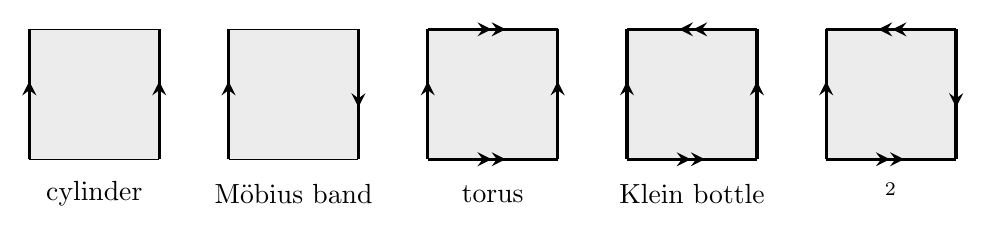
\begin{tikzpicture}[scale=1.1,>=stealth]
        % cylinder
        \begin{scope}
            \fill[gray!15] (0,0) rectangle (1.5,1.5);
            \draw (0,0)--(1.5,0) (0,1.5)--(1.5,1.5);
            \draw[very thick] (0,0)--(0,1.5) (1.5,0)--(1.5,1.5);
            \draw[very thick,->] (0,0.6)--(0,0.9);
            \draw[very thick,->] (1.5,0.6)--(1.5,0.9);
            \node at (0.75,-0.4) {cylinder};
        \end{scope}
        % Mobius
        \begin{scope}[shift={(2.3,0)}]
            \fill[gray!15] (0,0) rectangle (1.5,1.5);
            \draw (0,0)--(1.5,0) (0,1.5)--(1.5,1.5);
            \draw[very thick] (0,0)--(0,1.5) (1.5,0)--(1.5,1.5);
            \draw[very thick,->] (0,0.6)--(0,0.9);
            \draw[very thick,->] (1.5,0.9)--(1.5,0.6);
            \node at (0.75,-0.4) {M\"obius band};
        \end{scope}
        % torus
        \begin{scope}[shift={(4.6,0)}]
            \fill[gray!15] (0,0) rectangle (1.5,1.5);
            \draw[very thick] (0,0)--(0,1.5) (1.5,0)--(1.5,1.5);
            \draw[very thick] (0,0)--(1.5,0) (0,1.5)--(1.5,1.5);
            \draw[very thick,->] (0,0.6)--(0,0.9);
            \draw[very thick,->] (1.5,0.6)--(1.5,0.9);
            \draw[very thick,->>] (0.6,0)--(0.9,0);
            \draw[very thick,->>] (0.6,1.5)--(0.9,1.5);
            \node at (0.75,-0.4) {torus};
        \end{scope}
        % Klein
        \begin{scope}[shift={(6.9,0)}]
            \fill[gray!15] (0,0) rectangle (1.5,1.5);
            \draw[very thick] (0,0)--(0,1.5) (1.5,0)--(1.5,1.5);
            \draw[very thick] (0,0)--(1.5,0) (0,1.5)--(1.5,1.5);
            \draw[very thick,->] (0,0.6)--(0,0.9);
            \draw[very thick,->] (1.5,0.6)--(1.5,0.9);
            \draw[very thick,->>] (0.6,0)--(0.9,0);
            \draw[very thick,->>] (0.9,1.5)--(0.6,1.5);
            \node at (0.75,-0.4) {Klein bottle};
        \end{scope}
        % RP2
        \begin{scope}[shift={(9.2,0)}]
            \fill[gray!15] (0,0) rectangle (1.5,1.5);
            \draw[very thick] (0,0)--(0,1.5) (1.5,0)--(1.5,1.5);
            \draw[very thick] (0,0)--(1.5,0) (0,1.5)--(1.5,1.5);
            \draw[very thick,->] (0,0.6)--(0,0.9);
            \draw[very thick,->] (1.5,0.9)--(1.5,0.6);
            \draw[very thick,->>] (0.6,0)--(0.9,0);
            \draw[very thick,->>] (0.9,1.5)--(0.6,1.5);
            \node at (0.75,-0.4) {$\RP^2$};
        \end{scope}
    \end{tikzpicture}
    \caption{Gluing the sides of a square. Thick sides with the same kind of arrow (single or double) are identified so that the arrows match; thin sides are not glued.}
    \label{fig square gluings}
\end{figure}

\begin{example}[Collapsing a subspace]\label{example collapsing}\index{Collapsing a subspace}
    For $A\subset X$, the space $X/A$ is obtained by identifying all points of $A$ to a single point. For example, collapsing the boundary of the closed ball, $\wb{B^n}/\bbS^{n-1}$, produces the sphere $\bbS^n$: the map
    \[\wb{B^n}\to\bbS^n,\qquad \bf{x}\mapsto\Big(\sin(\pi\lvert \bf{x}\rvert)\frac{\bf{x}}{\lvert \bf{x}\rvert},\;-\cos(\pi\lvert \bf{x}\rvert)\Big)\]
    (extended by continuity to $\bf{x}=0$) sends the center to the south pole, wraps concentric spheres onto parallels of $\bbS^n$, and sends the whole boundary to the north pole. It descends to a continuous bijection $\wb{B^n}/\bbS^{n-1}\to\bbS^n$, which will turn out to be a homeomorphism by compactness (Example~\ref{example compact quotients}).
\end{example}

\begin{defn}[Orbit space]\index{Orbit space}
    Let a group $G$ act on a space $X$ by homeomorphisms. The \emph{orbit space} $X/G$ is the quotient of $X$ by the relation $x\sim gx$, $g\in G$, whose classes are the orbits $Gx$.
\end{defn}

The projection $\pi:X\to X/G$ is always an open map, because for open $U\subset X$ the set $\pi^{-1}(\pi(U))=\bigcup_{g\in G}gU$ is open. The examples $\bbR/\bbZ$ and $\bbR^n/\bbZ^n$ above are orbit spaces. Not all orbit spaces are this nice: the additive group $\bbQ$ acts on $\bbR$ by translations, and since each orbit $x+\bbQ$ is dense, every nonempty saturated open set is all of $\bbR$. So $\bbR/\bbQ$ carries the trivial topology.

\begin{example}[Projective spaces]\label{example projective spaces}\index{Projective space}
    The real projective space $\RP^n$ is the set of lines through the origin in $\bbR^{n+1}$. There are two natural ways to topologize it: as the orbit space $(\bbR^{n+1}\setminus\{0\})/\bbR^\times$ of the scaling action, or as the orbit space $\bbS^n/\{\pm1\}$ of the antipodal action on the sphere. These give the same space. The inclusion $\bbS^n\hookrightarrow\bbR^{n+1}\setminus\{0\}$ and the normalization $\bf{x}\mapsto \bf{x}/\lvert \bf{x}\rvert$ map orbits to orbits, so by the universal property they descend to continuous maps between the two orbit spaces, and these are inverse to each other. Similarly, the complex projective space $\CP^n=(\bbC^{n+1}\setminus\{0\})/\bbC^\times\cong\bbS^{2n+1}/\U_1$. For $n=2$, gluing the antipodal points on the boundary of the upper hemisphere (which is a disk) gives the description of $\RP^2$ in Figure~\ref{fig square gluings}.
\end{example}
In \Chap~\ref{ch manifolds}, we will see that $\RP^n$ is a smooth manifold (Examples~\ref{example topological manifolds} and~\ref{example smooth atlases}).

\begin{rem}
    In general, quotient spaces do not inherit good properties from the original space; $\bbR/\bbQ$ is an extreme case. Most of the time we will need to verify that a quotient is reasonable, and the separation axioms of \S\ref{Separation Axioms} are the tools for this.
\end{rem}

\subsection{Gluing}

\begin{defn}[Adjunction space]\index{Adjunction space}\index{Gluing}
    Let $A\subset X$ be a subspace and $f:A\to Y$ a continuous map. The space $Y\cup_fX$ obtained by \emph{attaching} $X$ to $Y$ along $f$ is the quotient of $X\sqcup Y$ by the relation $a\sim f(a)$ for $a\in A$.
\end{defn}

By the universal properties of the disjoint union and of the quotient, a map out of $Y\cup_fX$ is the same as a pair of continuous maps on $X$ and $Y$ that agree along $f$. In other words, $Y\cup_fX$ is the pushout of the inclusion $A\hookrightarrow X$ and $f$ in $\mathsf{Top}$ (Definition~\ref{pushouts}):
\[\begin{tikzcd}
    A\arrow[r,"f"]\arrow[d,hook] & Y\arrow[d]\\
    X\arrow[r] & Y\cup_fX
\end{tikzcd}\]
For example, gluing two closed disks along the identity map of their boundary circles produces a sphere (two hemispheres), and gluing the boundary circle of a disk to a point produces a sphere as well (Example~\ref{example collapsing}).

An especially important case is the gluing of \emph{open} pieces along open subsets. Let $U_1,U_2$ be spaces, $V_i\subset U_i$ open subsets, and $\varphi:V_1\to V_2$ a homeomorphism. The space $U_1\cup_\varphi U_2$ is the quotient of $U_1\sqcup U_2$ by $v\sim\varphi(v)$. Each $U_i$ is homeomorphic to an open subset of the result (Exercise~\ref{xca gluing open pieces}), so every point of $U_1\cup_\varphi U_2$ has a neighborhood looking exactly like an open set in $U_1$ or $U_2$.

\begin{example}[The sphere from two planes]\label{example sphere two charts}
    Take two copies of $\bbR^n$ and glue $\bbR^n\setminus\{0\}$ in the first to $\bbR^n\setminus\{0\}$ in the second by the inversion $\varphi(\bf{y})=\bf{y}/\lvert \bf{y}\rvert^2$. The result is homeomorphic to $\bbS^n$. Indeed, the stereographic projections $\varphi_N$ and $\varphi_S$ from the north and south poles (Example~\ref{example homeomorphisms}) identify the two copies of $\bbR^n$ with $\bbS^n\setminus\{N\}$ and $\bbS^n\setminus\{S\}$ (here $\varphi_S(\bf{x})=\frac{(x^1,\ldots,x^n)}{1+x^{n+1}}$), and one checks that $\varphi_S\circ\varphi_N^{-1}(\bf{y})=\bf{y}/\lvert \bf{y}\rvert^2$. The origin of the second copy is the ``point at infinity'' of the first.
\end{example}

\begin{example}[The line with two origins]\label{example two origins}\index{Line with two origins}
    Now glue two copies of $\bbR$ along $\bbR\setminus\{0\}$ by the \emph{identity} map. The result looks like a line, except that it has two origins $0_1$ and $0_2$ (Figure~\ref{fig two origins}). Every neighborhood of $0_1$ contains an interval $(-\epsilon,0)\cup\{0_1\}\cup(0,\epsilon)$, and similarly for $0_2$, so any two neighborhoods of the two origins intersect. The two origins cannot be separated, and a sequence like $1/k$ converges to both of them. Locally, the space looks like $\bbR$ everywhere, but it is clearly not the kind of space we want to study. The separation axioms of \S\ref{Separation Axioms} are designed to exclude such behavior.
\end{example}

\begin{figure}[tp]
    \centering
    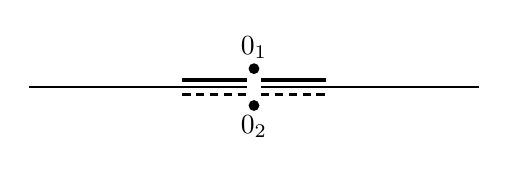
\begin{tikzpicture}[scale=1.3,>=stealth]
        \draw[thick] (-2.2,0)--(-0.07,0);
        \draw[thick] (0.07,0)--(2.2,0);
        \fill (0,0.18) circle (1.5pt) node[above]{$0_1$};
        \fill (0,-0.18) circle (1.5pt) node[below]{$0_2$};
        \draw[very thick] (-0.7,0.07)--(-0.07,0.07) (0.07,0.07)--(0.7,0.07);
        \draw[very thick,densely dashed] (-0.7,-0.07)--(-0.07,-0.07) (0.07,-0.07)--(0.7,-0.07);
    \end{tikzpicture}
    \caption{The line with two origins. Neighborhoods of $0_1$ (solid) and $0_2$ (dashed) always overlap.}
    \label{fig two origins}
\end{figure}

\begin{defn}[Wedge sum, smash product]\index{Wedge sum}\index{Smash product}
    For pointed spaces $(X,x_0)$ and $(Y,y_0)$, the \emph{wedge sum} is $X\vee Y=(X\sqcup Y)/(x_0\sim y_0)$, and the \emph{smash product} is $X\wedge Y=(X\times Y)/(X\vee Y)$, where $X\vee Y$ is identified with the subspace $(\{x_0\}\times Y)\cup(X\times\{y_0\})$. The wedge sum is the coproduct in the category $\mathsf{Top}_\bullet$ of pointed spaces.
\end{defn}

For example, $\bbS^1\vee\bbS^1$ is the figure eight, which is also the image of the curve in Figure~\ref{fig figure eight}.

\begin{rem}[Topologies from adjoints]
    The forgetful functor $\Box:\mathsf{Top}\to\mathsf{Set}$ has both a left and a right adjoint (Definition~\ref{defn adjoint functors}): the discrete topology $\mathrm{D}$ and the trivial topology $\mathrm{T}$, since every map out of a discrete space and every map into a trivial space is continuous:
    \[\Hom_{\mathsf{Top}}(\mathrm{D}(S),Y)\cong\mathrm{Map}(S,\Box Y),\qquad \mathrm{Map}(\Box X,S)\cong\Hom_{\mathsf{Top}}(X,\mathrm{T}(S)).\]
    As a consequence, $\Box$ preserves all limits and colimits (\S\ref{Limits and colimits}). This is why every product, fibered product, sum and quotient in $\mathsf{Top}$ has the set-theoretic one as its underlying set, and only the topology needs to be chosen -- which is exactly what initial and final topologies do.
\end{rem}

\begin{rem}[Regular monomorphisms and epimorphisms]
    The categorical notions of \S\ref{sec: classes of morphisms} do not distinguish embeddings from other injective maps: in $\mathsf{Top}$, monomorphisms are just the continuous injections. However, one can do better. The equalizer of two maps $f,g:X\to Y$ is the subspace $\{f=g\}\subset X$, and their coequalizer is the quotient of $Y$ by the finest equivalence relation with $f(x)\sim g(x)$. A monomorphism which is an equalizer of some pair of maps is called \emph{regular}, and similarly for epimorphisms and coequalizers. In $\mathsf{Top}$, the regular monomorphisms are exactly the embeddings (the image of an embedding $A\to X$ is the equalizer of its indicator function and the constant $1$, both viewed as maps into $\{0,1\}$ with the trivial topology), and the regular epimorphisms are exactly the quotient maps (a quotient map $\pi:X\to Y$ is the coequalizer of the two projections $X\times_YX\to X$).
\end{rem}

\begin{xca}
    Show that a continuous surjection that is open or closed is a quotient map, and that a composition of quotient maps is a quotient map.
\end{xca}
\begin{xca}
    Show that $\wb{A\times B}=\wb{A}\times\wb{B}$ in $X\times Y$. Conclude that products of closed sets are closed.
\end{xca}
\begin{xca}
    Show that $\rho(x,y)=\sum_k2^{-k}\min(1,\lvert x_k-y_k\rvert)$ is a metric on $\bbR^\bbN$ which induces the product topology.
\end{xca}
\begin{xca}\label{xca gluing open pieces}
    In the setting of gluing open pieces, show that the maps $U_i\to U_1\cup_\varphi U_2$ are homeomorphisms onto open subsets, and that the projection $U_1\sqcup U_2\to U_1\cup_\varphi U_2$ is open.
\end{xca}
\begin{xca}
    Show that there is a continuous bijection from the cone $(\bbS^{n-1}\times[0,1])/(\bbS^{n-1}\times\{0\})$ onto the closed ball $\wb{B^n}$. (Proposition~\ref{prop compact to Hausdorff} will show that it is a homeomorphism.)
\end{xca}
\begin{xca}\label{wedge sums}
    \begin{enumerate}
        \item Show that $\bbS^1\wedge \bbS^1=\bbT^2/(\bbS^1\vee\bbS^1)\cong \bbS^2$.
        \item More generally, show that $\bbS^m\wedge \bbS^n\cong \bbS^{m+n}$. \emph{Hint:} $\bbS^n$ is $\bbR^n$ with one point added at infinity (Example~\ref{example one point compactification}), and $\bbR^m\times\bbR^n=\bbR^{m+n}$.
    \end{enumerate}
\end{xca}


\section{Connectedness}\label{sec: connectedness}

The simplest topological invariant answers the question whether a space consists of one piece.

\begin{defn}[Connected space]\index{Connected space}
    A space $X$ is \emph{connected} if it is not the union of two disjoint nonempty open subsets. Equivalently, the only clopen subsets of $X$ are $\varnothing$ and $X$. A subset is connected if it is connected in the subspace topology.
\end{defn}

A decomposition $X=U\sqcup V$ into disjoint open sets is the same as a continuous map $f:X\to\{0,1\}$ into the two-point discrete space, namely $U=f^{-1}(0)$ and $V=f^{-1}(1)$. Thus
\begin{gather*}
    \boxed{X \text{ is connected iff every continuous map } X\to\{0,1\} \text{ is constant.}}
\end{gather*}
This reformulation makes most proofs about connectedness one-liners.

\begin{thm}\label{thm interval connected}\index{Interval!connectedness of}
    The interval $[a,b]\subset\bbR$ is connected.
\end{thm}
\begin{proof}
    Let $f:[a,b]\to\{0,1\}$ be continuous with $f(a)=0$, and let $s=\sup\{t\mid f=0\text{ on }[a,t]\}$. Since $f^{-1}(0)$ is closed, $f(s)=0$, and since it is open, $f=0$ on a neighborhood of $s$. If $s<b$, this contradicts the choice of $s$; so $s=b$ and $f\equiv0$.
\end{proof}

\begin{prop}\label{prop connected properties}
    \begin{enumerate}
        \item Continuous images of connected spaces are connected.
        \item If connected subsets $A_i\subset X$ all contain a common point, then $\bigcup_iA_i$ is connected.
        \item If $A$ is connected and $A\subset B\subset\wb{A}$, then $B$ is connected.
        \item Finite products of connected spaces are connected.
    \end{enumerate}
\end{prop}
\begin{proof}
    In each case let $f$ be a continuous map into $\{0,1\}$. (1) If $g:X\to Y$ is continuous and onto, then $f\circ g$ is constant, hence so is $f$. (2) $f$ is constant on each $A_i$, and the constants agree at the common point. (3) $f$ is constant on $A$, say $f=0$ there, and $f^{-1}(0)$ is closed, so it contains $\wb{A}\supset B$. (4) For $X\times Y$, the slices $\{x\}\times Y\cong Y$ and $X\times\{y\}\cong X$ are connected, so $f(x,y)=f(x,y_0)=f(x_0,y_0)$.
\end{proof}

In particular, connectedness is a topological invariant. Combining (1) with Theorem~\ref{thm interval connected} gives the intermediate value theorem: a continuous function $f:X\to\bbR$ on a connected space takes all values between any two of its values. In fact, the connected subsets of $\bbR$ are exactly the intervals (Exercise~\ref{xca connected subsets of R}). By (4), $\bbR^n$ is connected, and so is every ball, since it is homeomorphic to $\bbR^n$.

\begin{defn}[Connected components]\index{Connected component}
    Write $x\sim y$ if some connected subset of $X$ contains both $x$ and $y$. By Proposition~\ref{prop connected properties}(2) this is an equivalence relation, and its classes are called the \emph{connected components} of $X$.
\end{defn}

The component of $x$ is the union of all connected sets containing $x$, i.e., the largest connected set containing $x$. By Proposition~\ref{prop connected properties}(3), components are closed. Every clopen set is a union of components. A space is the disjoint union of its components, but this need not be a decomposition into \emph{open} sets: in $\bbQ\subset\bbR$, any subset with two points $p<q$ is split by an irrational number between them, so the components of $\bbQ$ are single points, none of which is open.

\subsection{Path-connectedness}

In practice, the most convenient way to show that something is connected is to connect its points by paths.

\begin{defn}[Paths, path-connectedness]\index{Path}\index{Path-connected space}
    A \emph{path} in $X$ from $x$ to $y$ is a continuous map $\gamma:[0,1]\to X$ with $\gamma(0)=x$ and $\gamma(1)=y$. The space $X$ is \emph{path-connected} if any two of its points can be joined by a path.
\end{defn}

Being joined by a path is an equivalence relation: paths can be reversed, $t\mapsto\gamma(1-t)$, and concatenated, by running through the first path at double speed and then through the second one. The equivalence classes are called \emph{path components}, and their set is denoted
\[\pi_0(X)=\{\text{path components of }X\}.\]
A continuous map $f:X\to Y$ sends paths to paths, so it induces a map $\pi_0(f):\pi_0(X)\to\pi_0(Y)$, and $\pi_0:\mathsf{Top}\to\mathsf{Set}$ is a functor. In particular, homeomorphic spaces have the same number of path components. This is our first, rather primitive, ``algebraic'' invariant.\index{$\pi_0$}

\begin{prop}
    Every path-connected space is connected.
\end{prop}
\begin{proof}
    Fix $x_0\in X$. Then $X$ is the union of the images of all paths starting at $x_0$, which are connected by Theorem~\ref{thm interval connected} and Proposition~\ref{prop connected properties}(1) and all contain $x_0$.
\end{proof}

\begin{example}\label{example path connected}
    \begin{enumerate}
        \item Convex subsets of $\bbR^n$ are path-connected by straight segments $\gamma(t)=(1-t)\bf{x}+t\bf{y}$.
        \item $\bbR^n\setminus\{0\}$ is path-connected for $n\geq2$: two points can be joined by a segment, or, if the segment passes through $0$, by two segments through a third point. Its image under the normalization $\bf{x}\mapsto \bf{x}/\lvert \bf{x}\rvert$ is the sphere $\bbS^{n-1}$, which is therefore path-connected for $n\geq 2$. For $n=1$, both $\bbR\setminus\{0\}$ and $\bbS^0=\{\pm1\}$ have two components.
        \item Products of path-connected spaces are path-connected: join $(x,y)$ to $(x',y')$ by the path $(\gamma_1(t),\gamma_2(t))$.
    \end{enumerate}
\end{example}

The converse of the proposition is false, and the standard counterexample shows what can go wrong.

\begin{example}[Topologist's sine curve]\label{example sine curve}\index{Topologist's sine curve}
    Let $\Gamma=\{(x,\sin\frac1x)\mid 0<x\leq1\}$ be the graph of $\sin\frac1x$, and $T=\Gamma\cup(\{0\}\times[-1,1])$ (Figure~\ref{tsine}). The graph $\Gamma$ is connected, being the image of $(0,1]$, and $\Gamma\subset T\subset\wb{\Gamma}$, so $T$ is connected by Proposition~\ref{prop connected properties}(3).

    However, $T$ is not path-connected. Suppose $c(t)=(x(t),y(t))$ is a path in $T$ from $(0,0)$ to $(1,\sin1)$. Let $t_0$ be the last moment when $c$ is on the vertical segment, so that $x(t_0)=0$ and $x(t)>0$ for $t>t_0$. By the intermediate value theorem, for every $\delta>0$ the function $x(t)$ takes all values in $(0,x(t_0+\delta)]$ on $(t_0,t_0+\delta]$. Hence $y(t)=\sin\frac{1}{x(t)}$ takes both values $\pm1$ on every such interval, and cannot be continuous at $t_0$. The problem is that $\sin\frac1x$ has no limit as $x\to0$: the graph oscillates infinitely often while approaching the segment, and a path would have to traverse all of these oscillations in finite time.
\end{example}

\begin{figure}[tp]
    \centering
    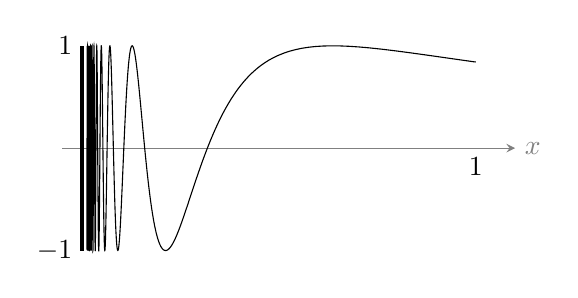
\begin{tikzpicture}[xscale=5,yscale=1.3,>=stealth]
        \draw[->,gray] (-0.05,0)--(1.1,0) node[right]{$x$};
        \draw[very thick] (0,-1)--(0,1);
        \draw[domain=1:80,samples=1500,variable=\u] plot ({1/\u},{sin(\u r)});
        \node[left] at (0,1) {$1$};
        \node[left] at (0,-1) {$-1$};
        \node[below] at (1,0) {$1$};
    \end{tikzpicture}
    \caption{The topologist's sine curve: the graph of $\sin\frac1x$ together with the segment $\{0\}\times[-1,1]$ (thick).}
    \label{tsine}
\end{figure}

For reasonable spaces, connectedness and path-connectedness coincide.

\begin{defn}[Local path-connectedness]\index{Locally path-connected space}
    A space is \emph{locally path-connected} if every neighborhood of every point contains a path-connected neighborhood of that point.
\end{defn}

For example, open subsets of $\bbR^n$ are locally path-connected, because balls are convex. The topologist's sine curve is not locally path-connected at the points of the segment.

\begin{lem}\label{lem locally path connected}
    In a locally path-connected space, path components are open and closed. Consequently, a connected, locally path-connected space is path-connected, and in general the components and path components of a locally path-connected space coincide.
\end{lem}
\begin{proof}
    If $x$ lies in a path component $C$, then a path-connected neighborhood of $x$ lies in $C$ as well, so $C$ is open. The complement of $C$ is the union of the other path components, hence also open. If $X$ is connected, the clopen set $C$ must be all of $X$.
\end{proof}

\begin{cor}\label{cor open connected Rn}
    A connected open subset $U\subset\bbR^n$ is path-connected. Moreover, any two of its points can be joined by a polygonal path in $U$.
\end{cor}
\begin{proof}
    Apply the argument of the lemma to the set of points that can be joined to a fixed point by a polygonal path. It is open and closed because balls are convex.
\end{proof}

\subsection{Applications}

Connectedness gives the first, and very simple, way to prove that spaces are \emph{not} homeomorphic: a homeomorphism $f:X\to Y$ restricts to a homeomorphism $X\setminus\{x\}\cong Y\setminus\{f(x)\}$, so the number of components that appear after removing a point is a topological invariant.

\begin{example}[Cut points]\label{example cut points}\index{Cut point}
    \begin{enumerate}
        \item $\bbR\not\cong\bbR^n$ for $n\geq2$: removing any point disconnects $\bbR$, but not $\bbR^n$ (Example~\ref{example path connected}).
        \item $[0,1]\not\cong\bbS^1$: removing an interior point disconnects the interval, while the circle minus any point is homeomorphic to an open interval.
        \item The cross $\bbR\times\{0\}\cup\{0\}\times\bbR$ is not homeomorphic to $\bbR$: removing its center produces four components, while removing any point of $\bbR$ produces two.
        \item The figure eight $\bbS^1\vee\bbS^1$ and the theta-shaped graph $\ominus$ are not homeomorphic: removing the center of the figure eight disconnects it, while $\ominus$ stays connected after removing any one of its points.
    \end{enumerate}
\end{example}

Unfortunately, this method stops working in higher dimensions: removing a point from $\bbR^2$ or from $\bbR^3$ leaves a connected space in both cases. We will need finer invariants, such as the fundamental group, to distinguish them (\S\ref{sec: fundamental group}).

Connectedness also gives useful information about matrix groups.

\begin{prop}\label{prop components of GLn}
    \begin{enumerate}
        \item $\GL_n(\bbC)$ is path-connected.
        \item $\SO_n$ is path-connected, and $\Or_n$ has exactly two path components, $\SO_n$ and $\{\det=-1\}$.
        \item $\GL_n(\bbR)$ has exactly two path components, $\{\det>0\}$ and $\{\det<0\}$.
    \end{enumerate}
\end{prop}
\begin{proof}
    (1) Given $A,B\in\GL_n(\bbC)$, consider the complex line of matrices $(1-z)A+zB$, $z\in\bbC$. The function $p(z)=\det((1-z)A+zB)$ is a polynomial in $z$ with $p(0)=\det A\neq0$, so it vanishes only at finitely many points. The plane $\bbC$ minus finitely many points is path-connected, so there is a path from $z=0$ to $z=1$ avoiding them, which gives a path from $A$ to $B$ in $\GL_n(\bbC)$.

    (2) By the normal form of orthogonal matrices, every $A\in\SO_n$ can be written as $A=QR_\theta Q^{-1}$, where $Q\in\Or_n$ and $R_\theta$ is block-diagonal with $2\times2$ rotation blocks by angles $\theta_1,\ldots,\theta_k$ and with $1$'s on the rest of the diagonal. Then $t\mapsto QR_{t\theta}Q^{-1}$, $t\in[0,1]$, is a path in $\SO_n$ from the identity to $A$. Multiplication by a fixed reflection maps $\SO_n$ homeomorphically onto $\{\det=-1\}$. The two sets are separated by the continuous function $\det:\Or_n\to\{\pm1\}$.

    (3) Since $\det:\GL_n(\bbR)\to\bbR\setminus\{0\}$ is continuous and onto, there are at least two components. Every $A$ with $\det A>0$ can be written as $A=QR$ by the Gram-Schmidt process, where $Q\in\SO_n$ and $R$ is upper triangular with positive diagonal entries. Such matrices $R$ form a convex set containing $\rmI_n$, so $t\mapsto Q((1-t)R+t\rmI_n)$ is a path in $\GL_n(\bbR)$ from $A$ to $Q$, which can then be joined to $\rmI_n$ by (2). The case $\det A<0$ follows by multiplying by a reflection.
\end{proof}

\begin{xca}\label{xca connected subsets of R}
    Show that a subset of $\bbR$ is connected iff it is an interval (i.e., contains $[x,y]$ together with any two of its points $x<y$).
\end{xca}
\begin{xca}
    Classify the capital letters of the Latin alphabet, drawn as unions of line segments and arcs in the plane, up to homeomorphism. \emph{Hint:} count the components that appear after removing various points.
\end{xca}
\begin{xca}
    Show that the complement of a countable set in $\bbR^n$, $n\geq2$, is path-connected.
\end{xca}
\begin{xca}
    Show that an open subset of $\bbR^n$ has at most countably many components.
\end{xca}
\begin{xca}
    Show that $\U_n$, $\SU_n$, and $\SL_n(\bbR)$ are path-connected.
\end{xca}


\section{Compactness}\label{sec: compactness}

Compactness is the topological substitute for finiteness. It is what makes a continuous function on a closed interval bounded, and what allows us to pass from local statements (true near every point) to global ones (true uniformly on the whole space).

\begin{defn}[Compactness]\index{Compact space}\index{Cover}
    A \emph{cover} of a space $X$ is a collection of subsets whose union is $X$; it is \emph{open} if all of its members are open. A space $X$ is \emph{compact} if every open cover of $X$ has a finite subcover. A subset of $X$ is compact if it is compact in the subspace topology, i.e., if every cover of it by open subsets of $X$ has a finite subcover.
\end{defn}

Finite spaces are compact, and $\bbR$ is not: the cover by the intervals $(-k,k)$ has no finite subcover. Neither is $(0,1]$: the cover by $(\frac1k,1]$ has no finite subcover, because the points close to $0$ ``escape''. The fundamental example is the closed interval.

\begin{thm}[Heine-Borel]\index{Theorem!Heine-Borel}\label{thm interval compact}
    The interval $[0,1]$ is compact.
\end{thm}
\begin{proof}
    Suppose an open cover $\mathscr{U}$ of $I_0=[0,1]$ has no finite subcover. Then one of the two halves of $I_0$ also has no finite subcover; call it $I_1$. Continuing, we get nested closed intervals $I_0\supset I_1\supset\ldots$ of lengths $2^{-k}$, none of which is covered by finitely many members of $\mathscr{U}$. They intersect in a point $x$ (completeness of $\bbR$). But $x$ lies in some $U\in\mathscr{U}$, and since $U$ is open, it contains all $I_k$ with $k$ large -- a cover by a single set.
\end{proof}

\begin{prop}\label{prop f(compact)=compact}
    \begin{enumerate}
        \item Continuous images of compact spaces are compact.
        \item Closed subsets of compact spaces are compact.
    \end{enumerate}
\end{prop}
\begin{proof}
    (1) If $f:X\to Y$ is continuous and $\mathscr{U}$ is an open cover of $f(X)$, then the preimages of its members form an open cover of $X$; a finite subcover of the latter gives a finite subcover of the former. (2) If $A\subset X$ is closed, add the open set $X\setminus A$ to any open cover of $A$ to get an open cover of $X$.
\end{proof}

Thus compactness is a topological invariant. Since a compact subset of $\bbR$ is bounded (it is covered by the intervals $(-k,k)$), we get the \emph{extreme value theorem}\index{Theorem!Extreme value}: a continuous function $f:X\to\bbR$ on a compact space is bounded. If $X\neq\varnothing$, it attains its maximum and minimum, because $\sup f(X)$ lies in $\wb{f(X)}$, which equals $f(X)$ as we will now see.

\subsection{Compactness and the Hausdorff property}

For compact sets to behave like closed bounded sets in $\bbR^n$, we need to exclude spaces like the line with two origins (Example~\ref{example two origins}). There, the compact interval $[-1,1]$ of the first copy of $\bbR$ is not closed, since $0_2$ lies in its closure.

\begin{defn}[Hausdorff space]\index{Hausdorff space}
    A space $X$ is \emph{Hausdorff} if any two distinct points $x\neq y$ have disjoint neighborhoods.
\end{defn}

Metric spaces are Hausdorff: take the balls of radius $\frac12\rho(x,y)$. Subspaces and products of Hausdorff spaces are clearly Hausdorff. In a Hausdorff space every sequence has at most one limit. The line with two origins is the simplest non-Hausdorff space. We will study this and related conditions in more detail in \S\ref{Separation Axioms}.

\begin{prop}\label{prop compact in Hausdorff}
    Let $X$ be a Hausdorff space.
    \begin{enumerate}
        \item Every compact subset $K\subset X$ is closed.
        \item Disjoint compact subsets $K,L\subset X$ have disjoint open neighborhoods.
    \end{enumerate}
\end{prop}
\begin{proof}
    (1) Let $x\notin K$. For each $y\in K$, choose disjoint open neighborhoods $U_y\ni y$ and $V_y\ni x$. Finitely many $U_{y_1},\ldots,U_{y_m}$ cover $K$, and then $V_{y_1}\cap\ldots\cap V_{y_m}$ is a neighborhood of $x$ disjoint from $K$. So $X\setminus K$ is open by Proposition~\ref{open iff contains neighborhoods}.

    (2) The same argument, with $x$ replaced by the compact set $L$, shows that each $y\in K$ has a neighborhood disjoint from some neighborhood of $L$. Now take a finite subcover of $K$ again.
\end{proof}

The following consequence is the main practical tool for proving that two spaces are homeomorphic; we will put it to work as soon as we have enough examples of compact spaces.

\begin{prop}\label{prop compact to Hausdorff}
    A continuous map $f:X\to Y$ from a compact space into a Hausdorff space is \emph{closed}\index{Closed map}, i.e., maps closed sets to closed sets. In particular:
    \begin{enumerate}
        \item a continuous bijection $X\to Y$ is a homeomorphism;
        \item a continuous injection $X\to Y$ is an embedding;
        \item a continuous surjection $X\to Y$ is a quotient map.
    \end{enumerate}
\end{prop}
\begin{proof}
    A closed set $F\subset X$ is compact, hence so is $f(F)$, which is therefore closed in $Y$. For a continuous bijection $f$, closedness of $f$ says exactly that $f^{-1}$ is continuous. The other two claims are proved in the same way.
\end{proof}

\subsection{Products and the Heine-Borel theorem}

\begin{lem}[Tube lemma]\label{lem tube}\index{Lemma!Tube}
    Let $K$ be compact and $W\subset X\times K$ an open set containing the slice $\{x\}\times K$. Then $W$ contains a whole ``tube'' $U\times K$, where $U$ is a neighborhood of $x$ (Figure~\ref{fig tube lemma}).
\end{lem}
\begin{proof}
    Every point $(x,k)$ has a box neighborhood $U_k\times V_k\subset W$. Finitely many $V_{k_1},\ldots,V_{k_m}$ cover $K$; take $U=U_{k_1}\cap\ldots\cap U_{k_m}$.
\end{proof}

\begin{figure}[tp]
    \centering
    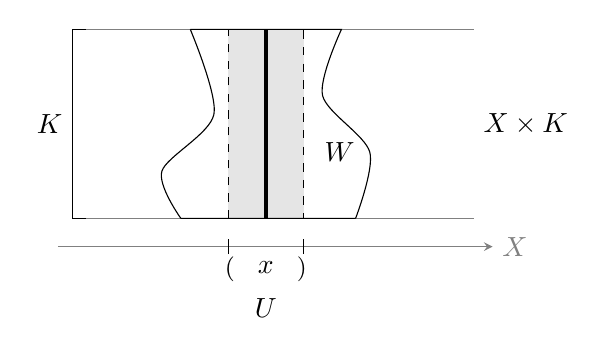
\begin{tikzpicture}[scale=1.2,>=stealth]
        \draw[->,gray] (-0.2,0)--(4.4,0) node[right]{$X$};
        \draw (0.1,0.3)--(-0.05,0.3)--(-0.05,2.3)--(0.1,2.3);
        \node[left] at (-0.05,1.3) {$K$};
        \fill[gray!20] (1.6,0.3) rectangle (2.4,2.3);
        \draw[dashed] (1.6,0.3) rectangle (2.4,2.3);
        \draw[very thick] (2,0.3)--(2,2.3);
        \draw[gray] (0.1,2.3)--(4.2,2.3) (0.1,0.3)--(4.2,0.3);
        \node[right] at (4.2,1.3) {$X\times K$};
        \draw (1.1,0.3)--(2.95,0.3) plot[smooth] coordinates {(2.95,0.3) (3.1,1.0) (2.6,1.6) (2.8,2.3)} -- (1.2,2.3) plot[smooth] coordinates {(1.2,2.3) (1.45,1.4) (0.9,0.8) (1.1,0.3)};
        \node at (2.78,1.0) {$W$};
        \node[below] at (2,-0.05) {$x$};
        \draw (1.6,-0.08)--(1.6,0.08) (2.4,-0.08)--(2.4,0.08);
        \node[below] at (1.62,0.0) {\small $($};
        \node[below] at (2.38,0.0) {\small $)$};
        \node at (2.0,-0.65) {$U$};
    \end{tikzpicture}
    \caption{The tube lemma: an open set $W$ containing the slice $\{x\}\times K$ (thick) contains a whole tube $U\times K$ (shaded).}
    \label{fig tube lemma}
\end{figure}

\begin{prop}\label{prop product compact}
    Finite products of compact spaces are compact.
\end{prop}
\begin{proof}
    Let $\mathscr{U}$ be an open cover of $X\times Y$ with $X,Y$ compact. For each $x$, the slice $\{x\}\times Y\cong Y$ is covered by finitely many members of $\mathscr{U}$, and by the tube lemma their union contains a tube $U_x\times Y$. Finitely many $U_x$ cover $X$, and the corresponding finitely many members of $\mathscr{U}$ cover $X\times Y$.
\end{proof}

In fact, \emph{arbitrary} products of compact spaces are compact. This is the \emph{Tychonoff theorem}\index{Theorem!Tychonoff}, which we will not need (see, e.g., \cite{Munk}).

\begin{thm}[Heine-Borel in $\bbR^n$]\label{thm Heine-Borel}
    A subset of $\bbR^n$ is compact iff it is closed and bounded.
\end{thm}
\begin{proof}
    A closed bounded set lies in some cube $[-R,R]^n$, which is compact by Theorem~\ref{thm interval compact} and Proposition~\ref{prop product compact}, so it is compact as a closed subset. Conversely, a compact set is covered by finitely many of the balls $B_k(0)$, hence bounded, and it is closed by Proposition~\ref{prop compact in Hausdorff}.
\end{proof}

\begin{example}\label{example compact groups}
    \begin{enumerate}
        \item Closed balls, spheres, tori $\bbT^n\subset\bbC^n$, and $\bbS^n/\{\pm1\}=\RP^n$ are compact.
        \item The groups $\Or_n$ and $\U_n$ are compact: they are closed (Example~\ref{example zero sets}) and bounded, since $\lVert A\rVert_{\mathrm{F}}^2=\tr A^\top A=n$ for $A\in\Or_n$. So are $\SO_n$ and $\SU_n$. On the other hand, for $n\geq2$ the group $\SL_n(\bbR)$ is unbounded (it contains $\diag(t,1/t,1,\ldots,1)$ for all $t>0$), and $\GL_n(\bbR)$ is not closed.
    \end{enumerate}
\end{example}

With these examples at hand, we can now settle several claims made earlier.

\begin{example}\label{example compact quotients}
    \begin{enumerate}
        \item The map $t\mapsto\rme^{2\pi\rmi t}$ descends to a continuous bijection $[0,1]/(0\sim1)\to\bbS^1$, hence a homeomorphism. Compare this with Example~\ref{example bijection not homeo}: it is the gluing of the endpoints that makes the inverse continuous.
        \item The continuous bijection $\wb{B^n}/\bbS^{n-1}\to\bbS^n$ of Example~\ref{example collapsing} is a homeomorphism. (The quotient is compact, being the image of the compact ball.)
        \item Similarly, the squares with glued sides in Figure~\ref{fig square gluings} map homeomorphically onto the cylinder $\bbS^1\times[0,1]$ and the torus $\bbT^2$, and the map $z\mapsto z^2$ induces a homeomorphism $\bbS^1/\{\pm1\}=\RP^1\cong\bbS^1$.
    \end{enumerate}
\end{example}

\begin{cor}[Norms on finite-dimensional spaces]\label{cor norms equivalent}\index{Norm!equivalence of}
    All norms on a finite-dimensional vector space are equivalent.
\end{cor}
\begin{proof}
    Choosing a basis, it suffices to compare a norm $\lVert\cdot\rVert$ on $\bbR^n$ with the Euclidean norm. By the triangle inequality and Cauchy-Schwarz, $\lVert \bf{x}\rVert\leq\sum_i\lvert x^i\rvert\lVert \bf{e}_i\rVert\leq C\lvert \bf{x}\rvert$. In particular, $\lVert\cdot\rVert$ is continuous with respect to the Euclidean metric, so it attains a minimum $m$ on the compact unit sphere $\bbS^{n-1}$, and $m>0$ since $\lVert\cdot\rVert$ vanishes only at $0$. By homogeneity, $\lVert \bf{x}\rVert\geq m\lvert \bf{x}\rvert$ for all $\bf{x}$.
\end{proof}

So in finite dimensions there is only one reasonable topology on a vector space, and every finite-dimensional normed space is homeomorphic (even linearly) to $\bbR^n$. In infinite dimensions, by contrast, closed and bounded sets are usually not compact.

\begin{example}[Non-compact unit balls]\label{example noncompact balls}
    \begin{enumerate}
        \item The unit vectors $e_k\in\ell^p$ satisfy $\lVert e_k-e_l\rVert_p=2^{1/p}$ for $k\neq l$. The open balls of radius $2^{1/p-1}$ around them are disjoint, so the cover of the closed unit ball by all balls of this radius has no finite subcover.
        \item In $C[0,1]$, take ``bumps'' $f_k$ of height $1$ supported on the intervals $[\frac{1}{k+1},\frac1k]$, whose interiors are disjoint. They lie in the closed unit ball and $\lVert f_k-f_l\rVert_\infty=1$ for $k\neq l$, so the same argument applies.
    \end{enumerate}
    In fact, the closed unit ball of a normed space is compact iff the space is finite-dimensional (\emph{Riesz's theorem}\index{Theorem!Riesz}). The idea is the same: in infinite dimensions one can always choose infinitely many unit vectors at mutual distances at least $\frac12$. Compactness in infinite dimensions therefore requires strong extra restrictions. A typical example is the \emph{Hilbert cube} $\{x\in\ell^2\mid\lvert x_k\rvert\leq1/k\}$, which is compact because its sides shrink fast enough (Exercise~\ref{xca Hilbert cube}).
\end{example}

\subsection{Compact metric spaces}

In metric spaces, compactness can be tested with sequences.

\begin{defn}[Sequential compactness]\index{Sequentially compact space}
    A space is \emph{sequentially compact} if every sequence in it has a convergent subsequence.
\end{defn}

\begin{lem}[Lebesgue number]\index{Lemma!Lebesgue}\index{Lebesgue number}\label{Lebesque lemma}
    Let $X$ be a sequentially compact metric space and $\mathscr{U}$ an open cover of $X$. Then there is a $\delta>0$ (a \emph{Lebesgue number} of $\mathscr{U}$) such that every subset of $X$ of diameter less than $\delta$ lies in a single member of $\mathscr{U}$.
\end{lem}
\begin{proof}
    Otherwise, for every $k$ there is a point $x_k$ such that the ball $B_{1/k}(x_k)$ is not contained in any member of $\mathscr{U}$. A subsequence converges to some $x$, which lies in some $U\in\mathscr{U}$ together with a ball $B_\epsilon(x)$. But then $B_{1/k}(x_k)\subset B_\epsilon(x)\subset U$ as soon as $\rho(x_k,x)<\epsilon/2$ and $1/k<\epsilon/2$.
\end{proof}

\begin{thm}\label{thm compact metric}
    A metric space is compact iff it is sequentially compact.
\end{thm}
\begin{proof}
    Let $X$ be compact and $(x_k)$ a sequence. If no subsequence converged, every point $x\in X$ would have a ball around it containing $x_k$ for only finitely many $k$. Finitely many of these balls cover $X$, which is absurd.

    Conversely, let $X$ be sequentially compact and $\mathscr{U}$ an open cover with Lebesgue number $\delta$. It suffices to cover $X$ by finitely many balls of radius $\delta/3$, since each of them lies in a member of $\mathscr{U}$. If this were impossible, we could inductively choose points $x_1,x_2,\ldots$ with $x_{k+1}\notin B_{\delta/3}(x_1)\cup\ldots\cup B_{\delta/3}(x_k)$. Their mutual distances are at least $\delta/3$, so no subsequence converges.
\end{proof}

A metric space that can be covered by finitely many $\epsilon$-balls for every $\epsilon>0$ is called \emph{totally bounded}\index{Totally bounded space}, and compact spaces obviously have this property. We return to it in \S\ref{sec: completeness}.

\begin{defn}[Uniform continuity]\index{Uniform continuity}
    A map $f:X\to Y$ between metric spaces is \emph{uniformly continuous} if for every $\epsilon>0$ there is a $\delta>0$ such that $\rho_X(x,x')<\delta$ implies $\rho_Y(f(x),f(x'))<\epsilon$ for \emph{all} $x,x'\in X$.
\end{defn}

\begin{prop}\label{prop uniform continuity}
    Every continuous map from a compact metric space to a metric space is uniformly continuous.
\end{prop}
\begin{proof}
    Given $\epsilon>0$, let $\delta$ be a Lebesgue number of the open cover by the sets $f^{-1}(B_{\epsilon/2}(y))$, $y\in Y$. If $\rho(x,x')<\delta$, then $x,x'$ lie in one of these sets, so $\rho(f(x),f(x'))<\epsilon$.
\end{proof}

For example, $x\mapsto 1/x$ is continuous but not uniformly continuous on $(0,1]$, and $x\mapsto x^2$ is not uniformly continuous on $\bbR$. On compact sets, such ``runaway'' behavior is impossible.

\subsection{Local compactness and compactification}

\begin{defn}[Local compactness]\index{Locally compact space}
    A space is \emph{locally compact} if every point has a compact neighborhood.
\end{defn}

The spaces $\bbR^n$ and all of their open and closed subsets are locally compact, and so are all compact spaces. By Riesz's theorem, an infinite-dimensional normed space is not locally compact. In a locally compact Hausdorff space, every point $x$ has an open neighborhood with compact closure: if $K$ is a compact neighborhood of $x$ and $V\subset K$ an open neighborhood, then $\wb{V}\subset K$ because $K$ is closed (Proposition~\ref{prop compact in Hausdorff}), so $\wb{V}$ is compact. In fact, every neighborhood $W$ of $x$ contains a compact neighborhood of $x$. We may assume that $W\subset V$ is open. Then $x$ and the compact set $\wb{V}\setminus W$ have disjoint neighborhoods $U_1$ and $U_2$ (Proposition~\ref{prop compact in Hausdorff}), and the closure of $U_1\cap W$ is a compact neighborhood of $x$: it lies in $\wb{V}$ and avoids $U_2$, hence lies in $W$.

A non-compact space ``leaks'' to infinity, and it is often useful to plug the leak by adding a point.

\begin{defn}[One-point compactification]\index{One-point compactification}\index{Compactification!one-point}
    Let $X$ be a locally compact Hausdorff space. Its \emph{one-point compactification} is $X^+=X\sqcup\{\infty\}$, whose open sets are the open subsets of $X$ together with the sets $(X\setminus K)\cup\{\infty\}$, $K\subset X$ compact.
\end{defn}

One checks directly that this is a topology, that $X^+$ is compact (any open set containing $\infty$ misses only a compact part of $X$) and Hausdorff (a point $x\in X$ is separated from $\infty$ by a neighborhood with compact closure), and that $X\subset X^+$ is an open subspace.

\begin{example}\label{example one point compactification}
    \begin{enumerate}
        \item The inverse stereographic projection $\varphi_N^{-1}:\bbR^n\to\bbS^n\setminus\{N\}$ extends to a continuous bijection $(\bbR^n)^+\to\bbS^n$ sending $\infty$ to $N$. Indeed, if $W$ is an open neighborhood of $N$, then $\bbS^n\setminus W$ is compact, hence so is its preimage $K\subset\bbR^n$, and the preimage of $W$ is $(\bbR^n\setminus K)\cup\{\infty\}$. By Proposition~\ref{prop compact to Hausdorff}, $(\bbR^n)^+\cong\bbS^n$. For $n=2$, the compactification $\bbC^+=\bbC\cup\{\infty\}\cong\bbS^2$ is the \emph{Riemann sphere}.\index{Riemann sphere}
        \item The one-point compactification of the discrete space $\bbN$ is homeomorphic to $\{\frac1k\mid k\in\bbN\}\cup\{0\}\subset\bbR$.
    \end{enumerate}
\end{example}

\begin{defn}[Proper map]\index{Proper map}
    A continuous map $f:X\to Y$ is \emph{proper} if the preimage of every compact set is compact.
\end{defn}

A proper map sends ``infinity to infinity'': points escaping every compact set in $X$ are mapped to points escaping every compact set in $Y$. Homeomorphisms, inclusions of closed subsets, and nonconstant polynomials $p:\bbC\to\bbC$ (since $\lvert p(z)\rvert\to\infty$ as $\lvert z\rvert\to\infty$) are proper. The projection $\bbR^2\to\bbR$ and the map $\bbR\to\bbS^1$, $t\mapsto\rme^{2\pi\rmi t}$, are not.

\begin{prop}\label{prop proper closed}
    A proper map $f:X\to Y$ between locally compact Hausdorff spaces extends to a continuous map $f^+:X^+\to Y^+$ with $f^+(\infty)=\infty$, and it is closed.
\end{prop}
\begin{proof}
    The preimage under $f^+$ of a neighborhood $(Y\setminus K)\cup\{\infty\}$ of $\infty$ is $(X\setminus f^{-1}(K))\cup\{\infty\}$, which is open precisely because $f$ is proper. If $F\subset X$ is closed, then $F\cup\{\infty\}$ is closed in $X^+$, so its image $f(F)\cup\{\infty\}$ is closed in $Y^+$ by Proposition~\ref{prop compact to Hausdorff}. Intersecting with $Y$, we see that $f(F)$ is closed.
\end{proof}

In particular, the image of a proper map is closed. For a nonconstant complex polynomial this gives one half of a proof of the fundamental theorem of algebra, the other half being that the image is also open. (We will give a different proof in Corollary~\ref{cor FTA}.)

Finally, a non-compact space can often be approximated from within by compact sets. This allows one to run compactness arguments step by step, and to measure convergence of functions ``on compact sets'' by countably many numbers (\S\ref{sec: completeness}).

\begin{prop}[Compact exhaustion]\label{prop compact exhaustion}\index{Exhaustion by compact sets}
    Let $X$ be a locally compact Hausdorff space that is a countable union of compact sets $C_1,C_2,\ldots$ (for example, a second countable one). Then there are compact sets $K_1\subset K_2\subset\ldots$ with $K_n\subset\Int K_{n+1}$ and $\bigcup_nK_n=X$.
\end{prop}
\begin{proof}
    Every compact set $C$ has an open neighborhood with compact closure: cover $C$ by finitely many open sets with compact closures. Let $K_1=C_1$, and let $K_{n+1}$ be the closure of such a neighborhood of $K_n\cup C_{n+1}$. If $X$ is second countable, the closures of those elements of a countable basis that have compact closure are a countable family of compact sets covering $X$.
\end{proof}
On manifolds, such exhaustions can even be described as the sublevel sets of a smooth function (Proposition~\ref{prop.exhaustion}).

For an open set $U\subset\bbR^n$, one can simply take $K_n=\{\bf{x}\in U\mid\lvert \bf{x}\rvert\leq n,\ \dist(\bf{x},\bbR^n\setminus U)\geq\frac1n\}$.

\begin{rem}
    Compact Hausdorff spaces can be completely recovered from the algebra $C(X)$ of continuous functions on them. The points $x\in X$ correspond to the maximal ideals $\{f\mid f(x)=0\}$. Compactness guarantees that there are no others: if an ideal $I$ is not contained in any of these, then for each $x$ there is $f_x\in I$ with $f_x(x)\neq0$; finitely many of the open sets $\{f_x\neq0\}$ cover $X$, and then $\sum_i\lvert f_{x_i}\rvert^2\in I$ is invertible, so $I=C(X)$. This is the starting point of the duality between compact Hausdorff spaces and commutative $C^\ast$-algebras mentioned in Example~\ref{example Gelfand duality}.
\end{rem}

\begin{xca}
    Show that a finite union of compact subsets is compact, and that a closed discrete subset of a compact space is finite.
\end{xca}
\begin{xca}\label{xca Hilbert cube}
    Show that the Hilbert cube $\{x\in\ell^2\mid\lvert x_k\rvert\leq 1/k\}$ is compact. \emph{Hint:} use Theorem~\ref{thm compact metric} and a diagonal subsequence.
\end{xca}
\begin{xca}
    Show that a map $f:X\to Y$ between metric spaces is continuous iff its restriction to every compact subset is continuous. (This fails for general topological spaces.)
\end{xca}
\begin{xca}
    Show that the composition of proper maps is proper, and that the projection $X\times K\to X$ is proper if $K$ is compact.
\end{xca}
\begin{xca}
    Show that a compact metric space is separable, and that a locally compact, separable metric space is a countable union of compact sets.
\end{xca}


\section{Completeness and function spaces}\label{sec: completeness}

Compactness is a topological property, but much of analysis rests on a property that depends on the metric itself: the convergence of sequences whose terms get closer and closer to each other.

\begin{defn}[Completeness]\index{Cauchy sequence}\index{Complete metric space}
    A sequence $(x_k)$ in a metric space is a \emph{Cauchy sequence} if for every $\epsilon>0$ there is $N$ such that $\rho(x_k,x_l)<\epsilon$ for all $k,l>N$. A metric space is \emph{complete} if every Cauchy sequence in it converges.
\end{defn}

Every convergent sequence is Cauchy, by the triangle inequality. The real line is complete; this is one of the ways to state the completeness axiom of $\bbR$, and it is what we used in the proof of Theorem~\ref{thm interval compact}. Since a sequence in $\bbR^n$ is Cauchy iff its coordinates are, $\bbR^n$ is complete as well, and by Corollary~\ref{cor norms equivalent} so is every finite-dimensional normed space. A subset of a complete space is complete iff it is closed. On the other hand, $\bbQ$ and $(0,1)$ are not complete.

\begin{example}[Completeness is not a topological property]\label{example N metrics}
    \begin{enumerate}
        \item The open interval $(0,1)$ is incomplete, but it is homeomorphic to the complete space $\bbR$.
        \item Consider three metrics on the set $\bbN$ of positive integers:
        \[\rho_1(m,n)=1,\qquad \rho_2(m,n)=\Big\lvert\frac1m-\frac1n\Big\rvert,\qquad \rho_3(m,n)=1+\frac{1}{m+n}\qquad (m\neq n).\]
        (The triangle inequality for $\rho_3$ holds because any two of its values add up to at least $2$, while all of them are at most $\frac32$.) In all three metrics, every point is isolated: for $\rho_2$, the ball of radius $\frac1n-\frac1{n+1}$ around $n$ is $\{n\}$. So all three define the \emph{discrete} topology on $\bbN$. Nevertheless, $\rho_1$ and $\rho_3$ are complete, because in them a Cauchy sequence must be eventually constant, while $\rho_2$ is not: the sequence $x_n=n$ is Cauchy, but it ``wants to converge'' to a missing point $\infty$ (Figure~\ref{fig N metric}).
    \end{enumerate}
\end{example}

\begin{figure}[tp]
    \centering
    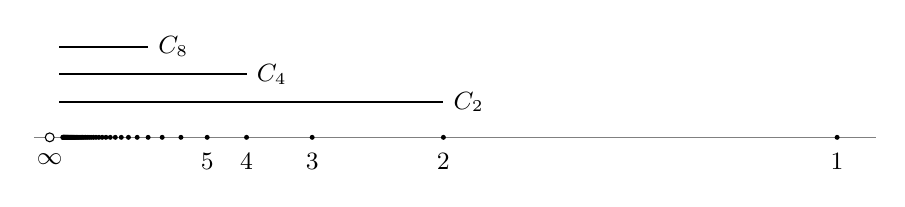
\begin{tikzpicture}[>=stealth]
        \draw[gray] (-0.2,0)--(10.5,0);
        \foreach \n in {1,...,60} { \fill ({10/\n},0) circle (0.9pt); }
        \foreach \n in {1,2,3,4,5} { \node[below] at ({10/\n},-0.08) {\small $\n$}; }
        \draw[fill=white] (0,0) circle (1.6pt);
        \node[below] at (0,-0.08) {\small $\infty$};
        \draw[thick] (0.12,0.45)--(5,0.45) node[right]{\small $C_2$};
        \draw[thick] (0.12,0.8)--(2.5,0.8) node[right]{\small $C_4$};
        \draw[thick] (0.12,1.15)--(1.25,1.15) node[right]{\small $C_8$};
    \end{tikzpicture}
    \caption{The metric $\rho_2(m,n)=\lvert\frac1m-\frac1n\rvert$ places $n\in\bbN$ at the point $\frac1n$ of the real line. The nested closed sets $C_k=\{n\geq k\}$ have diameters tending to zero, but they close in on the missing point $\infty$, so their intersection is empty.}
    \label{fig N metric}
\end{figure}

The following theorem is the reason why complete spaces are convenient: to find a point, it suffices to localize it more and more precisely.

\begin{thm}[Cantor's intersection theorem]\index{Theorem!Cantor's intersection}\label{thm Cantor intersection}
    Let $X$ be a complete metric space and $C_1\supset C_2\supset\ldots$ nonempty closed subsets with $\mathrm{diam}\,C_k\to0$. Then $\bigcap_kC_k$ consists of exactly one point.
\end{thm}
\begin{proof}
    Choose $x_k\in C_k$. For $k,l>N$ both points lie in $C_N$, so $\rho(x_k,x_l)\leq\mathrm{diam}\,C_N$, and the sequence is Cauchy. Its limit $x$ lies in every $C_N$, since $C_N$ is closed and contains $x_k$ for $k\geq N$. Two points of the intersection are at distance at most $\mathrm{diam}\,C_k\to0$.
\end{proof}

Both hypotheses are essential, as the metrics on $\bbN$ from Example~\ref{example N metrics} show. In all of them, the sets $C_k=\{n\geq k\}$ are closed, nonempty, nested, and have empty intersection.
\begin{itemize}
    \item For $\rho_2$, the diameters $\mathrm{diam}\,C_k=\frac1k$ tend to zero, but the space is not complete (Figure~\ref{fig N metric}). The same happens with balls: $B_{1/k}(k)=\{n>k/2\}$ is a decreasing sequence of balls whose radii tend to zero and whose intersection is empty.
    \item For $\rho_3$, the space is complete, but $\mathrm{diam}\,C_k=1+\frac1{2k+1}$ does not tend to zero. Note that $C_k$ is the closed ball $\wb{B}_{r_k}(k)$ of radius $r_k=1+\frac{1}{2k}$, so here we have a \emph{decreasing sequence of nested closed balls in a complete space with empty intersection}. In $\bbR^n$ this is impossible even if the radii do not tend to zero, because closed balls there are compact (Exercise~\ref{xca nested compact}).
\end{itemize}

Completeness also gives the metric characterization of compactness, separating it into an ``analytic'' and a ``geometric'' part.

\begin{thm}\label{thm compact complete totally bounded}
    A metric space is compact iff it is complete and totally bounded.
\end{thm}
\begin{proof}
    If $X$ is compact, it is totally bounded (\S\ref{sec: compactness}), and a Cauchy sequence has a convergent subsequence by Theorem~\ref{thm compact metric}, so it converges itself. Conversely, given a sequence in a totally bounded space, infinitely many of its terms lie in one of finitely many balls of radius $1$, infinitely many of those in one of finitely many balls of radius $\frac12$, and so on. Choosing one term at each stage gives a Cauchy subsequence, which converges by completeness.
\end{proof}

\begin{rem}[Completion]\index{Completion}
    Every metric space $X$ is a dense subspace of a complete metric space $\wh{X}$, unique up to isometry, called its \emph{completion}. Its points are the Cauchy sequences in $X$, where two sequences are identified if their distance tends to zero. This is how $\bbR$ is obtained from $\bbQ$. The completion of $(\bbN,\rho_2)$ is $\bbN\cup\{\infty\}\cong\{\frac1n\}\cup\{0\}$, and the completion of $C[0,1]$ in the norm $\lVert\cdot\rVert_1$ is the space $L^1[0,1]$ of Lebesgue integrable functions.
\end{rem}

\subsection{Banach spaces}

\begin{defn}[Banach space]\index{Banach space}
    A \emph{Banach space} is a complete normed vector space.
\end{defn}

In a Banach space, every absolutely convergent series $\sum_kv_k$, i.e., one with $\sum_k\lVert v_k\rVert<\infty$, converges, because its partial sums form a Cauchy sequence: $\lVert\sum_{k=m}^nv_k\rVert\leq\sum_{k=m}^n\lVert v_k\rVert$.

\begin{prop}\label{prop C(K) complete}
    For a compact space $K$, the space $C(K)$ of continuous real functions with the sup norm is a Banach space. In other words, a uniform limit of continuous functions is continuous.
\end{prop}
\begin{proof}
    If $(f_k)$ is Cauchy in the sup norm, then each sequence $f_k(x)$ is Cauchy, and we let $f(x)=\lim_kf_k(x)$. Letting $l\to\infty$ in $\lvert f_k(x)-f_l(x)\rvert<\epsilon$ shows that $f_k\to f$ uniformly. Now $f$ is continuous at every $x$: take $k$ with $\lVert f-f_k\rVert_\infty<\epsilon/3$, and a neighborhood $U$ of $x$ on which $f_k$ varies by less than $\epsilon/3$; then $f$ varies by less than $\epsilon$ on $U$.
\end{proof}

Similarly, the sequence spaces $\ell^p$ and $\ell^\infty$ are Banach spaces (Exercise~\ref{xca lp complete}), and so is $c_0$, being a closed subspace of $\ell^\infty$.

\begin{example}[Choosing the right norm]\label{example C1 norm}
    The space $C^1[-1,1]$ of continuously differentiable functions is \emph{not} complete with the sup norm. The smooth functions $f_\epsilon(x)=\sqrt{x^2+\epsilon}$ satisfy $\lvert f_\epsilon(x)-\lvert x\rvert\rvert\leq\sqrt\epsilon$, so they converge uniformly to $\lvert x\rvert$, which is not differentiable. The sup norm simply does not see derivatives. With the norm $\lVert f\rVert_{C^1}=\lVert f\rVert_\infty+\lVert f'\rVert_\infty$, however, $C^1[-1,1]$ is complete. If $(f_k)$ is Cauchy in this norm, then $f_k\to f$ and $f'_k\to g$ uniformly, and passing to the limit in $f_k(x)=f_k(0)+\int_0^xf'_k$ gives $f(x)=f(0)+\int_0^xg$, so that $f'=g$ is continuous.
\end{example}

In finite dimensions every linear subspace is closed. In infinite dimensions this fails: by the Weierstrass approximation theorem, the polynomials form a dense subspace of $C[0,1]$, which is certainly not all of $C[0,1]$.

\begin{defn}[Bounded operators]\index{Operator norm}\index{Bounded operator}
    A linear map $A:V\to W$ between normed spaces is \emph{bounded} if its \emph{operator norm}
    \[\lVert A\rVert=\sup_{v\neq0}\frac{\lVert Av\rVert}{\lVert v\rVert}\]
    is finite. The bounded operators form a normed space $\mathcal{L}(V,W)$, and $\lVert AB\rVert\leq\lVert A\rVert\,\lVert B\rVert$.
\end{defn}

A linear map is bounded iff it is continuous: a bounded map is Lipschitz with constant $\lVert A\rVert$, and conversely, if $A$ is continuous at $0$, then $\lVert v\rVert\leq\delta$ implies $\lVert Av\rVert\leq1$, and by homogeneity $\lVert A\rVert\leq1/\delta$. By Corollary~\ref{cor norms equivalent}, all linear maps between finite-dimensional spaces are bounded, and for the Euclidean norms, $\lVert\cdot\rVert$ is the operator norm $\lVert\cdot\rVert_{\mathrm{op}}$ of Example~\ref{example matrix norms}. In infinite dimensions there are unbounded operators: differentiation $f\mapsto f'$ from $C^1[0,1]$ to $C[0,1]$, both with the sup norm, maps the functions $\sin kx$ of norm at most $1$ to functions of norm $k$.

\begin{example}[Matrix exponential and Neumann series]\label{example Neumann series}\index{Neumann series}\index{Matrix exponential}
    \begin{enumerate}
        \item For a matrix (or a bounded operator on a Banach space $V$, the space $\mathcal{L}(V,V)$ of which is again a Banach space, see Exercise~\ref{xca lp complete}) $A$, we have $\lVert A^k/k!\rVert\leq\lVert A\rVert^k/k!$, so the series $\rme^A=\sum_{k\geq0}\frac{A^k}{k!}$ converges absolutely, and $\lVert\rme^A\rVert\leq\rme^{\lVert A\rVert}$.
        \item If $\lVert B\rVert<1$, the geometric (\emph{Neumann}) series $\sum_{k\geq0}B^k$ converges, and multiplying it by $\rmI-B$ shows that it is the inverse of $\rmI-B$.
        \item Consequently, if $A$ is invertible and $\lVert H\rVert<1/\lVert A^{-1}\rVert$, then $A+H=A(\rmI+A^{-1}H)$ is invertible. Thus $\GL_n(\bbR)$ is open in $\Mat_n(\bbR)$ and contains an explicit ball around each of its points. The same holds for the invertible bounded operators on a Banach space, where we cannot use the determinant. Moreover, the series gives
        \[\lVert(A+H)^{-1}-A^{-1}\rVert\leq\frac{\lVert A^{-1}\rVert^2\lVert H\rVert}{1-\lVert A^{-1}\rVert\,\lVert H\rVert}\xrightarrow[H\to0]{}0,\]
        so inversion $A\mapsto A^{-1}$ is continuous.
    \end{enumerate}
\end{example}

\begin{example}[Matrix norms in infinite dimensions]\label{example trace class}
    For a real sequence $\lambda=(\lambda_k)$, consider the diagonal operator $D_\lambda(x)_k=\lambda_kx_k$ on $\ell^2$. In analogy with Example~\ref{example matrix norms}, its operator, Hilbert-Schmidt and trace norms are
    \[\lVert D_\lambda\rVert_{\mathrm{op}}=\sup_k\lvert\lambda_k\rvert,\qquad\lVert D_\lambda\rVert_{\mathrm{F}}=\Big(\sum_k\lambda_k^2\Big)^{1/2},\qquad\lVert D_\lambda\rVert_{\mathrm{tr}}=\sum_k\lvert\lambda_k\rvert.\]
    The identity operator ($\lambda_k=1$) is bounded but has infinite Hilbert-Schmidt norm, and $\lambda_k=\frac1k$ gives a Hilbert-Schmidt operator that is not of \emph{trace class}\index{Trace class operator}. The constants $\sqrt n$ and $n$ in the inequalities of Example~\ref{example equivalent norms} blow up, and the three norms define strictly nested classes of operators.
\end{example}

\subsection{Fixed points and the Baire theorem}

The two most useful consequences of completeness are the following.

\begin{thm}[Contraction mapping principle]\index{Theorem!Contraction mapping}\index{Contraction mapping principle}\label{thm contraction}
    Let $X$ be a nonempty complete metric space and $T:X\to X$ a \emph{contraction}\index{Fixed point}, i.e., $\rho(Tx,Ty)\leq q\,\rho(x,y)$ for some $q<1$. Then $T$ has a unique fixed point $x_\ast$. For every $x_0\in X$, the iterates $x_k=T^kx_0$ converge to $x_\ast$, and $\rho(x_k,x_\ast)\leq\frac{q^k}{1-q}\rho(x_1,x_0)$.
\end{thm}
\begin{proof}
    We have $\rho(x_{k+1},x_k)\leq q^k\rho(x_1,x_0)$, so by the triangle inequality and the geometric series, $\rho(x_k,x_l)\leq\frac{q^k}{1-q}\rho(x_1,x_0)$ for $l>k$. Thus $(x_k)$ is Cauchy, its limit $x_\ast$ satisfies $Tx_\ast=x_\ast$ by continuity of $T$, and letting $l\to\infty$ gives the error estimate. Two fixed points satisfy $\rho(x_\ast,y_\ast)\leq q\rho(x_\ast,y_\ast)$, hence coincide.
\end{proof}
We will use this principle to prove the inverse function theorem (Theorem~\ref{InMT}).

\begin{example}\label{example contractions}
    \begin{enumerate}
        \item The map $\cos$ sends $[0,1]$ into itself and $\lvert\cos x-\cos y\rvert\leq\sin 1\cdot\lvert x-y\rvert$ there. So the equation $\cos x=x$ has a unique solution in $[0,1]$, found by pressing the $\cos$ button on a calculator repeatedly.
        \item \emph{Newton's method}\index{Newton's method} for $\sqrt2$ iterates $T(x)=\frac12(x+\frac2x)$. On $[1,2]$ we have $\lvert T'(x)\rvert\leq\frac12$ and $T([1,2])\subset[1,2]$, so the iteration converges, in fact much faster than the theorem predicts.
        \item \emph{Kepler's equation} $E-e\sin E=M$ relates the eccentric anomaly $E$ of a planet to its mean anomaly $M$ (essentially, time) on an orbit of eccentricity $e<1$. It has a unique solution $E$ for each $M$, because $E\mapsto M+e\sin E$ is a contraction of $\bbR$ with $q=e$.
        \item \emph{Picard iteration}\index{Picard iteration}. The initial value problem $y'=y$, $y(0)=1$ is equivalent to the integral equation $y(t)=1+\int_0^ty(s)\dd s$. On the Banach space $C[0,a]$ with $a<1$, the right-hand side is a contraction with $q=a$. Starting from $y_0=1$, the iterates are the Taylor polynomials $\sum_{k\leq n}t^k/k!$, which converge to the unique solution $\rme^t$.
    \end{enumerate}
\end{example}

A subset of a space is \emph{nowhere dense}\index{Nowhere dense set} if its closure has empty interior. Points in $\bbR$, lines in $\bbR^2$, and proper linear subspaces of $\bbR^n$ are nowhere dense. A complete metric space cannot be ``built'' out of countably many such thin pieces.

\begin{thm}[Baire category theorem]\index{Theorem!Baire category}\label{thm Baire}
    In a complete metric space $X$, a countable intersection $\bigcap_kU_k$ of open dense sets is dense. Equivalently, a countable union of closed sets with empty interiors has empty interior. In particular, a nonempty $X$ is not a countable union of nowhere dense sets.
\end{thm}
\begin{proof}
    Let $W$ be a nonempty open set. Since $U_1$ is open and dense, $W\cap U_1$ contains a closed ball $\wb{B}_{r_1}(x_1)$ with $r_1<1$. Since $U_2$ is open and dense, $B_{r_1}(x_1)\cap U_2$ contains a closed ball $\wb{B}_{r_2}(x_2)$ with $r_2<\frac12$, and so on. By Cantor's intersection theorem, the nested closed balls meet in a point of $W\cap\bigcap_kU_k$. The other statements follow by taking complements.
\end{proof}

\begin{example}\label{example Baire}
    \begin{enumerate}
        \item $\bbR$ is uncountable, since points are nowhere dense.
        \item $\bbR^n$ is not a countable union of proper linear (or affine) subspaces.
        \item The space $\bbR[x]$ of real polynomials has no complete norm: it is the countable union of the finite-dimensional, hence closed, subspaces of polynomials of degree at most $n$, all of which have empty interior.
    \end{enumerate}
\end{example}

\subsection{Spaces of continuous maps}

Spaces of functions are themselves important topological spaces, and their compact subsets are characterized by the following theorem. A family $F$ of functions on a metric space $X$ is \emph{equicontinuous}\index{Equicontinuity} if for every $\epsilon>0$ there is a $\delta>0$ such that $\rho(x,x')<\delta$ implies $\lvert f(x)-f(x')\rvert<\epsilon$ for all $f\in F$ simultaneously.

\begin{thm}[Arzel\`a-Ascoli]\index{Theorem!Arzel\`a-Ascoli}\label{thm Arzela-Ascoli}
    Let $X$ be a compact metric space. A subset $F\subset C(X)$ has compact closure in the sup norm iff it is bounded and equicontinuous.
\end{thm}
\begin{proof}[Sketch of proof]
    Necessity follows from total boundedness of $\wb{F}$. For sufficiency, take a sequence $(f_k)$ in $F$ and a countable dense subset $\{x_1,x_2,\ldots\}\subset X$. By boundedness and a diagonal argument, we can pass to a subsequence that converges at every $x_i$. Equicontinuity and compactness of $X$ then make this subsequence uniformly Cauchy: on a small ball around each of finitely many $x_i$, all $f_k$ vary by less than $\epsilon$. By Proposition~\ref{prop C(K) complete}, it converges uniformly.
\end{proof}

For example, the functions $f:[0,1]\to[-1,1]$ with Lipschitz constant at most $L$ form a compact subset of $C[0,1]$, while the tent spikes of Example~\ref{example tent spikes} are bounded but not equicontinuous. This theorem is the basic tool for producing solutions of differential equations as limits of approximate solutions.

For general spaces $X$ and $Y$ there is no sup norm, but there is still a natural topology on $C(X,Y)$.

\begin{defn}[Compact-open topology]\index{Topology!compact-open}\label{defn compact-open}
    The \emph{compact-open topology} on $Y^X=C(X,Y)$ is generated by the sets
    \[M(K,U)=\{f\in C(X,Y)\mid f(K)\subset U\},\qquad K\subset X\text{ compact},\ U\subset Y\text{ open}.\]
\end{defn}

\begin{prop}\label{prop compact-open}
    \begin{enumerate}
        \item If $Y$ is Hausdorff, then $C(X,Y)$ is Hausdorff.
        \item If $X$ is compact and $Y$ is a metric space, the compact-open topology is the topology of the sup metric $\rho(f,g)=\sup_x\rho_Y(f(x),g(x))$, i.e., of uniform convergence.
    \end{enumerate}
\end{prop}
\begin{proof}
    (1) Let $f\neq g$, so that $f(x)\neq g(x)$ for some $x\in X$, and choose disjoint open neighborhoods $U_1$ of $f(x)$ and $U_2$ of $g(x)$. The one-point set $K=\{x\}$ is compact, so $M(K,U_1)$ and $M(K,U_2)$ are disjoint open neighborhoods of $f$ and $g$.

    (2) If $f\in M(K,U)$, then the compact set $f(K)$ has positive distance $\delta$ from $Y\setminus U$, so the sup-ball of radius $\delta$ around $f$ lies in $M(K,U)$. Conversely, given $f$ and $\epsilon>0$, cover the compact set $f(X)$ by finitely many balls $B_{\epsilon/3}(y_i)$ and let $K_i=f^{-1}(\wb{B}_{\epsilon/3}(y_i))$, $U_i=B_{\epsilon/2}(y_i)$. Then $f\in\bigcap_iM(K_i,U_i)$, and every $g$ in this intersection satisfies $\rho(f(x),g(x))<\frac{\epsilon}{3}+\frac{\epsilon}{2}<\epsilon$ for all $x$.
\end{proof}

Similarly, for a locally compact Hausdorff space $X$ and a metric space $Y$, the compact-open topology is the topology of uniform convergence on compact subsets, which for $X=\bbR^n$ can be described by the metric $\sum_m2^{-m}\min(1,\sup_{K_m}\lvert f-g\rvert)$ built from a compact exhaustion (Proposition~\ref{prop compact exhaustion}).

\begin{xca}\label{xca nested compact}
    Show that in a compact space, every decreasing sequence of nonempty closed sets has nonempty intersection. Conclude that a metric space is sequentially compact iff every decreasing sequence of nonempty closed subsets has nonempty intersection.
\end{xca}
\begin{xca}\label{xca lp complete}
    Show that $\ell^p$, $1\leq p\leq\infty$, are Banach spaces, and that $\mathcal{L}(V,W)$ is a Banach space whenever $W$ is.
\end{xca}
\begin{xca}
    Show that if $T:X\to X$ is a map of a complete metric space such that some iterate $T^m$ is a contraction, then $T$ has a unique fixed point. Use this to show that Picard iteration for $y'=y$, $y(0)=1$, converges on $C[0,a]$ for every $a>0$.
\end{xca}
\begin{xca}
    Show that $\rme^{A+B}=\rme^A\rme^B$ for commuting matrices $A,B$, and that $t\mapsto\rme^{tA}$ is continuous.
\end{xca}
\begin{xca}
    Use the Baire theorem to show that a nonempty complete metric space without isolated points is uncountable.
\end{xca}


\section{Separation axioms} \label{Separation Axioms}

Metric spaces have many properties that general topological spaces lack, and we have already met spaces, such as the line with two origins or the orbit space $\bbR/\bbQ$, which are too coarse to be useful. Such spaces arise naturally from quotient constructions, so we need criteria for excluding them. The \emph{separation axioms} measure how well open sets can tell points and closed sets apart.

\begin{defn}[Separation axioms]\index{Separation axioms}\index{Kolmogorov space}\index{Regular space}\index{Normal space}
    A topological space $X$ is called
    \begin{enumerate}
        \item $T_0$ (or \emph{Kolmogorov}) if for any two distinct points, one of them has a neighborhood not containing the other;
        \item $T_1$ if for any two distinct points, each of them has a neighborhood not containing the other;
        \item $T_2$ (or \emph{Hausdorff}) if any two distinct points have disjoint neighborhoods;
        \item \emph{regular} if it is $T_1$ and every point $x$ and closed set $F$ with $x\notin F$ have disjoint neighborhoods;
        \item \emph{normal} if it is $T_1$ and any two disjoint closed sets have disjoint neighborhoods.
    \end{enumerate}
    (The separation properties of regular and normal spaces without the $T_1$ condition are often called $T_3$ and $T_4$.)
\end{defn}

\begin{figure}[tp]
    \centering
    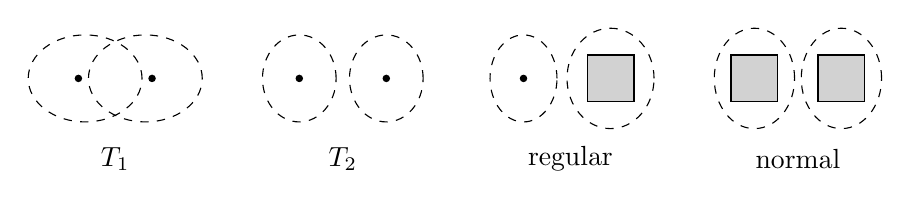
\begin{tikzpicture}[scale=0.85,>=stealth]
        \begin{scope}
            \draw[dashed] (-0.45,0) ellipse (0.85 and 0.65);
            \draw[dashed] (0.45,0) ellipse (0.85 and 0.65);
            \fill (-0.55,0) circle (1.6pt);
            \fill (0.55,0) circle (1.6pt);
            \node at (0,-1.2) {$T_1$};
        \end{scope}
        \begin{scope}[shift={(3.4,0)}]
            \draw[dashed] (-0.65,0) ellipse (0.55 and 0.65);
            \draw[dashed] (0.65,0) ellipse (0.55 and 0.65);
            \fill (-0.65,0) circle (1.6pt);
            \fill (0.65,0) circle (1.6pt);
            \node at (0,-1.2) {$T_2$};
        \end{scope}
        \begin{scope}[shift={(6.8,0)}]
            \draw[dashed] (-0.7,0) ellipse (0.5 and 0.65);
            \draw[dashed] (0.6,0) ellipse (0.65 and 0.75);
            \fill (-0.7,0) circle (1.6pt);
            \fill[gray!35] (0.25,-0.35) rectangle (0.95,0.35);
            \draw (0.25,-0.35) rectangle (0.95,0.35);
            \node at (0,-1.2) {regular};
        \end{scope}
        \begin{scope}[shift={(10.2,0)}]
            \draw[dashed] (-0.65,0) ellipse (0.6 and 0.75);
            \draw[dashed] (0.65,0) ellipse (0.6 and 0.75);
            \fill[gray!35] (-1.0,-0.35) rectangle (-0.3,0.35);
            \draw (-1.0,-0.35) rectangle (-0.3,0.35);
            \fill[gray!35] (0.3,-0.35) rectangle (1.0,0.35);
            \draw (0.3,-0.35) rectangle (1.0,0.35);
            \node at (0,-1.2) {normal};
        \end{scope}
    \end{tikzpicture}
    \caption{Separation axioms. Dots are points, shaded squares are closed sets, and dashed ovals are open neighborhoods.}
    \label{fig separation axioms}
\end{figure}

A space is $T_1$ iff its points are closed, since $X\setminus\{y\}$ is a neighborhood of each $x\neq y$ iff it is open. Since regular and normal spaces are $T_1$ by definition, we get the hierarchy
\[\text{normal}\implies\text{regular}\implies\text{Hausdorff}\implies T_1\implies T_0.\]
Metric spaces have all of these properties (see below). The Sierpi\'nski space of Example~\ref{example topologies} is $T_0$ but not $T_1$, and the line with two origins (Example~\ref{example two origins}) is $T_1$ but not Hausdorff. There are also Hausdorff spaces that are not regular, and regular spaces that are not normal, but they will play no role for us. In practice, the only separation axiom we will have to check is the Hausdorff property, which we introduced in \S\ref{sec: compactness}.

\subsection{The Hausdorff property}

\begin{prop}\label{prop Hausdorff diagonal}\index{Hausdorff space!diagonal criterion}
    A space $X$ is Hausdorff iff the diagonal $\Delta=\{(x,x)\}$ is closed in $X\times X$. Consequently, if $Y$ is Hausdorff and $f,g:X\to Y$ are continuous, then the \emph{coincidence set} $\{x\mid f(x)=g(x)\}$ is closed, and so is the graph $\{(x,f(x))\}\subset X\times Y$.
\end{prop}
\begin{proof}
    A basic neighborhood $U\times V$ of a point $(x,y)$ misses $\Delta$ iff $U\cap V=\varnothing$. The coincidence set is the preimage of $\Delta$ under $(f,g):X\to Y\times Y$, and the graph is the preimage of $\Delta$ under $f\times\id:X\times Y\to Y\times Y$.
\end{proof}

In particular, continuous maps into a Hausdorff space that agree on a dense subset agree everywhere, generalizing Proposition~\ref{prop dense determines maps}. Thus $\bbQ\hookrightarrow\bbR$ is an epimorphism in the category of Hausdorff topological rings. In the full subcategory $\mathsf{Haus}$\index{Category!of Hausdorff spaces} of Hausdorff spaces, this means that every continuous map with dense image is an epimorphism (and one can show that these are all epimorphisms in $\mathsf{Haus}$). So $\mathsf{Haus}$, unlike $\mathsf{Top}$, has non-surjective epimorphisms, such as $\bbQ\hookrightarrow\bbR$.

The Hausdorff property is inherited by subspaces and products, but not by quotients, which is where the trouble usually comes from. The next two results are the main tools for checking it.

\begin{prop}[Hausdorff quotients]\label{prop Hausdorff quotients}
    Let $\pi:X\to X/{\sim}$ be a quotient map, and $R=\{(x,x')\mid x\sim x'\}\subset X\times X$.
    \begin{enumerate}
        \item If $X/{\sim}$ is Hausdorff, then $R$ is closed.
        \item If $\pi$ is open (e.g., for orbit spaces) and $R$ is closed, then $X/{\sim}$ is Hausdorff.
        \item If $X$ is compact Hausdorff and $R$ is closed, then $X/{\sim}$ is Hausdorff.
    \end{enumerate}
\end{prop}
\begin{proof}
    (1) $R$ is the preimage of the diagonal under $\pi\times\pi$. (2) The map $\pi\times\pi$ is then open and surjective, and it maps the open complement of $R$ onto the complement of the diagonal, which is therefore open. (3) The quotient map is closed: if $F\subset X$ is closed, its saturation $\pi^{-1}(\pi(F))$ is the projection of the compact set $R\cap(X\times F)$ to the first factor, hence compact and closed. So points of $X/{\sim}$ are closed, and two of them have disjoint compact preimages $K,L$. By Proposition~\ref{prop compact in Hausdorff}, $K$ and $L$ have disjoint open neighborhoods $U,V$. Shrinking them to the saturated open sets $X\setminus\pi^{-1}(\pi(X\setminus U))$ and $X\setminus\pi^{-1}(\pi(X\setminus V))$, we obtain disjoint neighborhoods of the two points.
\end{proof}

\begin{example}\label{example RPn Hausdorff}
    \begin{enumerate}
        \item The antipodal relation on $\bbS^n$ is closed, so $\RP^n=\bbS^n/\{\pm1\}$ is compact Hausdorff. The same argument works for any finite group acting on a compact Hausdorff space, and for $\CP^n=\bbS^{2n+1}/\U_1$.
        \item For $\bbR/\bbQ$, the relation $R=\{(x,y)\mid x-y\in\bbQ\}$ is dense in $\bbR^2$, so it is very far from being closed.
    \end{enumerate}
\end{example}

For spaces glued from open pieces, the criterion takes a particularly geometric form.

\begin{prop}\label{prop Hausdorff gluing}
    Let $U_1,U_2$ be Hausdorff spaces, $V_i\subset U_i$ open, and $\varphi:V_1\to V_2$ a homeomorphism. Then $U_1\cup_\varphi U_2$ is Hausdorff iff the graph $\Gamma_\varphi=\{(v,\varphi(v))\}$ is closed in $U_1\times U_2$.
\end{prop}
\begin{proof}
    Points of the same piece can be separated within that piece, which is an open subset of the result (Exercise~\ref{xca gluing open pieces}). A point $x\in U_1$ and a point $y\in U_2$ that are not glued, i.e., $(x,y)\notin\Gamma_\varphi$, have disjoint neighborhoods iff they have product neighborhoods $U\times V$ disjoint from $\Gamma_\varphi$.
\end{proof}

In Example~\ref{example sphere two charts}, the graph of the inversion $\bf{y}\mapsto \bf{y}/\lvert \bf{y}\rvert^2$ is closed in $\bbR^n\times\bbR^n$: as $\bf{y}$ approaches $0$, its image escapes to infinity, so the graph has no limit points with $\bf{y}=0$. Thus the sphere is Hausdorff, as it should be. For the line with two origins, the graph of $\id_{\bbR\setminus\{0\}}$ has the limit point $(0,0)$, which lies outside the graph, and the two origins cannot be separated. The Hausdorff property of a glued space is therefore a condition on the gluing map near the boundary of its domain.

\begin{example}[Non-Hausdorff orbit spaces of continuous actions]\label{example non-Hausdorff orbit spaces}
    Non-Hausdorff quotients appear naturally in geometry.
    \begin{enumerate}
        \item The group $\bbR_{>0}$ acts on $\bbR^2\setminus\{0\}$ by $\lambda\cdot(x,y)=(\lambda x,\lambda^{-1}y)$. Its orbits are the branches of the hyperbolas $xy=c\neq0$ and the four open half-axes (Figure~\ref{fig hyperbolic orbits}). The positive $x$- and $y$-half-axes cannot be separated in the orbit space: every neighborhood of the point $(1,0)$ and every neighborhood of $(0,1)$ meet the hyperbolas $xy=c$ for all small $c>0$. In the first quadrant, the orbit space looks like a half-line $c\geq0$ with two endpoints, exactly as in the line with two origins.
        \item The group $\bbR$ acts on the torus $\bbT^2$ by $t\cdot(z,w)=(\rme^{2\pi\rmi t}z,\rme^{2\pi\rmi\alpha t}w)$ with $\alpha$ irrational (an ``irrational winding''). Every orbit is dense (Example~\ref{example not embeddings}), so the orbit space carries the trivial topology.
    \end{enumerate}
\end{example}

\begin{figure}[tp]
    \centering
    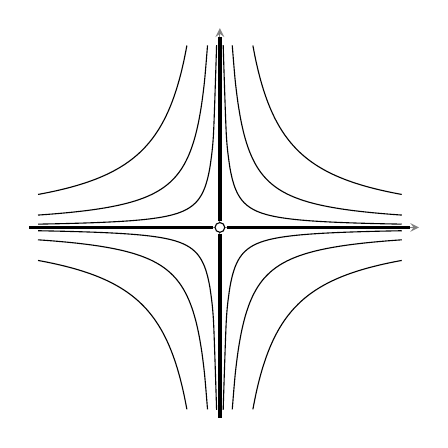
\begin{tikzpicture}[scale=1.1,>=stealth]
        \draw[->,gray] (-2.2,0)--(2.3,0);
        \draw[->,gray] (0,-2.2)--(0,2.3);
        \draw[very thick] (0.08,0)--(2.2,0) (-0.08,0)--(-2.2,0) (0,0.08)--(0,2.2) (0,-0.08)--(0,-2.2);
        \foreach \c in {0.08,0.3,0.8} {
            \draw[domain={\c/2.1}:2.1,samples=60,smooth,variable=\x] plot (\x,{\c/\x});
            \draw[domain={\c/2.1}:2.1,samples=60,smooth,variable=\x] plot (-\x,{-\c/\x});
            \draw[domain={\c/2.1}:2.1,samples=60,smooth,variable=\x] plot (-\x,{\c/\x});
            \draw[domain={\c/2.1}:2.1,samples=60,smooth,variable=\x] plot (\x,{-\c/\x});
        }
        \draw[fill=white] (0,0) circle (1.6pt);
    \end{tikzpicture}
    \caption{Orbits of $(x,y)\mapsto(\lambda x,\lambda^{-1}y)$ on the punctured plane. The hyperbolas $xy=c$ with small $c>0$ come close to both positive half-axes (thick), so these two orbits cannot be separated in the orbit space.}
    \label{fig hyperbolic orbits}
\end{figure}

\subsection{Normal spaces and Urysohn's lemma}

Normality is the separation property that allows us to construct many continuous functions.

\begin{prop}\label{prop metric normal}
    Metric spaces and compact Hausdorff spaces are normal.
\end{prop}
\begin{proof}
    For disjoint nonempty closed sets $A,B$ in a metric space (if one of them is empty, there is nothing to prove), the function
    \[f(x)=\frac{\dist(x,A)}{\dist(x,A)+\dist(x,B)}\]
    is continuous, equals $0$ exactly on $A$ (Proposition~\ref{prop closure}), and equals $1$ exactly on $B$. The sets $\{f<\frac12\}$ and $\{f>\frac12\}$ are disjoint open neighborhoods of $A$ and $B$. For compact Hausdorff spaces, closed sets are compact, and the claim is Proposition~\ref{prop compact in Hausdorff}(2).
\end{proof}

In metric spaces we have thus separated closed sets by a continuous function. Remarkably, the much weaker condition of normality already suffices for this.

\begin{thm}[Urysohn's lemma]\index{Lemma!Urysohn}\label{thm Urysohn lemma}
    If $X$ is normal and $A,B\subset X$ are disjoint closed sets, then there is a continuous function $f:X\to[0,1]$ with $\restr{f}{A}=0$ and $\restr{f}{B}=1$.
\end{thm}
\begin{proof}[Sketch of proof]
    Normality is equivalent to the following: if $F\subset U$ with $F$ closed and $U$ open, there is an open $V$ with $F\subset V\subset\wb{V}\subset U$. Using this repeatedly, construct open sets $U_r$ indexed by the dyadic rationals $r\in(0,1]$, with $A\subset U_r$, $U_1=X\setminus B$, and $\wb{U_r}\subset U_s$ for $r<s$: first $U_{1/2}$ between $A$ and $U_1$, then $U_{1/4}$ and $U_{3/4}$, and so on. Then $f(x)=\inf\{r\mid x\in U_r\}$ (with $f=1$ outside all $U_r$) is the required function. The sets $U_r$ are its ``sublevel sets'', and the nesting of their closures guarantees continuity.
\end{proof}
For manifolds, there is also a much simpler smooth version (Corollary~\ref{cor smooth Urysohn}).

Conversely, a function as in the lemma separates $A$ and $B$ by the open sets $\{f<\frac12\}$ and $\{f>\frac12\}$. A closely related result is the following.

\begin{thm}[Tietze extension theorem]\index{Theorem!Tietze extension}
    If $X$ is normal and $A\subset X$ is closed, then every continuous function $A\to\bbR$ extends to a continuous function $X\to\bbR$.
\end{thm}

Finally, we can answer the question of which spaces come from metrics.

\begin{thm}[Urysohn metrization theorem]\index{Theorem!Urysohn metrization}\index{Metrizable space}
    Every regular, second countable space is metrizable.
\end{thm}

The idea of the proof is as follows. A regular second countable space can be shown to be normal. One then uses Urysohn functions for pairs of basis elements $\wb{B_i}\subset B_j$ to construct countably many continuous functions $f_k:X\to[0,1]$ that separate points from closed sets. Then $x\mapsto(f_k(x)/k)_k$ is an embedding of $X$ into the Hilbert cube $\{x\in\ell^2\mid\lvert x_k\rvert\leq1/k\}$, and $X$ inherits the metric of $\ell^2$. For details we refer to \cite{Munk}.

\begin{xca}
    Show that a space is regular iff it is $T_1$ and every neighborhood of a point contains a closed neighborhood of that point.
\end{xca}
\begin{xca}
    Show that the quotient of a Hausdorff space by the action of a finite group is Hausdorff.
\end{xca}
\begin{xca}
    Glue two copies of $\bbR$ along the open set $(0,\infty)$ by the identity map. Is the result Hausdorff? What if we glue along $(0,\infty)$ using $x\mapsto 1/x$?
\end{xca}
\begin{xca}
    Show that the orbit space of $\bbR_{>0}$ acting on $\bbR^n\setminus\{0\}$ by scalar multiplication is homeomorphic to $\bbS^{n-1}$. Compare with Example~\ref{example non-Hausdorff orbit spaces}.
\end{xca}


\section{Homotopy}\label{sec.homotopy}

Homeomorphism is a very rigid relation, and topological invariants that can actually be computed are usually insensitive to much cruder deformations. A disk can be shrunk to a point, and the punctured plane can be squeezed onto a circle. The language for such deformations is homotopy.

\begin{defn}[Homotopy]\index{Homotopy}
    Two continuous maps $f_0,f_1:X\to Y$ are \emph{homotopic}, written $f_0\sim f_1$, if there is a continuous map $F:[0,1]\times X\to Y$, called a \emph{homotopy}, such that $F(0,x)=f_0(x)$ and $F(1,x)=f_1(x)$. We think of the first argument as time and of $F$ as a continuous family of maps $f_t=F(t,\cdot)$ interpolating between $f_0$ and $f_1$. If $A\subset X$ and $f_t(a)$ does not depend on $t$ for all $a\in A$, the homotopy is said to be \emph{relative to $A$}. A map homotopic to a constant map is called \emph{null-homotopic}\index{Null-homotopic map}\index{Relative homotopy}.
\end{defn}

\begin{prop}\label{prop homotopy equivalence relation}
    Homotopy (relative to $A$) is an equivalence relation on $C(X,Y)$, compatible with composition: if $f\sim f'$ and $g\sim g'$, then $g\circ f\sim g'\circ f'$.
\end{prop}
\begin{proof}
    Reflexivity and symmetry are clear ($F(1-t,x)$ reverses a homotopy). For transitivity, run the two homotopies one after the other at double speed. The result is continuous because its restrictions to the closed sets $[0,\frac12]\times X$ and $[\frac12,1]\times X$ are continuous and agree on their intersection, so the preimage of a closed set is a union of two closed sets. For composition, use $(t,x)\mapsto G(t,F(t,x))$.
\end{proof}

The set of homotopy classes of maps $X\to Y$ is denoted $[X,Y]$. By the proposition, homotopy classes can be composed, which gives the \emph{homotopy category} $\mathsf{hTop}$\index{Category!homotopy} whose objects are spaces and whose morphisms are homotopy classes of maps.

\begin{example}\label{example homotopies}
    \begin{enumerate}
        \item \emph{Straight-line homotopy.} Any two maps $f,g:X\to C$ into a convex subset $C$ of $\bbR^n$ (or of any normed space) are homotopic via $F(t,x)=(1-t)f(x)+tg(x)$.
        \item \emph{Maps into spheres.} If $f,g:X\to\bbS^n$ are never antipodal, i.e., $f(x)\neq-g(x)$ for all $x$, then they are homotopic: the straight segment from $f(x)$ to $g(x)$ avoids the origin, so we can project it back to the sphere,
        \[F(t,x)=\frac{(1-t)f(x)+tg(x)}{\lvert(1-t)f(x)+tg(x)\rvert}.\]
        In particular, maps with $\lvert f(x)-g(x)\rvert<2$ for all $x$ are homotopic, and a map $X\to\bbS^n$ that misses some point $\bf{p}$ is null-homotopic (it is never antipodal to the constant map $-\bf{p}$).
    \end{enumerate}
\end{example}

The second example illustrates a general principle: maps that are close to each other are homotopic. Behind it lies the idea that a homotopy is nothing but a continuous path in the space of maps. To make this precise, we need to know how the compact-open topology (Definition~\ref{defn compact-open}) interacts with maps of several variables.

\begin{prop}
    If $X$ is a locally compact Hausdorff space, then the evaluation map $e:Y^X\times X\to Y$, defined by $e(f,x)=f(x)$, is continuous.
\end{prop}
\begin{proof}
    Let $U$ be an open neighborhood of $f(x)$. Since $f$ is continuous and $X$ is locally compact (\S\ref{sec: compactness}), there is a compact neighborhood $K$ of $x$ such that $f(K)\subset U$. Thus $f\in M(K,U)$ and $M(K,U)\times K$ is mapped into $U$ by the evaluation map $e$. Finally, $M(K,U)\times K \subset Y^X\times X$ is a neighborhood of $(f,x)$. This proves continuity.
\end{proof}

\begin{thm}[{{\cite[Thm.~VII.2.4]{Bredon}}}]\label{compact open continuity}
    Let $X$ be a locally compact Hausdorff space, and $Y$ and $T$ Hausdorff spaces. For any map $f:X\times T\to Y$, denote $f_t(x)=f(x,t)$. Then the continuity of $f$ is equivalent to each $f_t$ being continuous separately and the mapping $t\mapsto f_t$ also being continuous from $T$ into $Y^X$. 
\end{thm}

This theorem implies that if $X$ is locally compact Hausdorff and $Y$ is Hausdorff, then a homotopy $X\times [0,1]\to Y$ is the same thing as a path $[0,1]\to Y^X$.
\begin{cor}[The Exponential Law {{\cite[Thm.~VII.2.5]{Bredon}}}]\label{cor exponential law}\index{Exponential law}
    Let $X,T$ be locally compact Hausdorff spaces, and $Y$ a Hausdorff space. Then the bijection from Theorem~\ref{compact open continuity} is a natural homeomorphism $Y^{X\times T}\cong \left(Y^X\right)^T$ taking $f$ to $f^\ast$ defined as $f^\ast (t)(x)=f(x,t)=f_t(x)$.
\end{cor}

Under similar conditions, one can also show that there are homeomorphisms $Y^X\times W^X\cong (Y\times W)^X$ (under $f\times g$) and $Y^{X\sqcup T}\cong Y^X\times Y^T$ (under $f\sqcup g$), and that for locally compact $Y$ the composition map $Z^Y\times Y^X \to Z^X$, $(f,g)\mapsto f\circ g$, is continuous. For details see \cite[\S VII.2]{Bredon}.

In particular, for compact Hausdorff $X$ and metric $Y$, a homotopy is a path in the sup metric (Proposition~\ref{prop compact-open}), and $[X,Y]=\pi_0(C(X,Y))$ is the set of path components of the space of maps.

\begin{defn}[Homotopy equivalence]\index{Homotopy equivalence}\index{Contractible space}
    A continuous map $f:X\to Y$ is a \emph{homotopy equivalence} if there is a map $g:Y\to X$ with $g\circ f\sim\id_X$ and $f\circ g\sim\id_Y$, i.e., if $f$ is an isomorphism in $\mathsf{hTop}$. In this case $X$ and $Y$ are \emph{homotopy equivalent}, $X\simeq Y$. A space homotopy equivalent to a point is called \emph{contractible}. In the category of pointed spaces, all maps and homotopies are required to preserve the basepoints.
\end{defn}

A space $X$ is contractible iff $\id_X$ is null-homotopic, i.e., homotopic to a constant map $x\mapsto x_0$. A contractible space is path-connected: the homotopy $F$ from the constant map to $\id_X$ moves $x_0$ to any given $x$ along the path $t\mapsto F(t,x)$. By Example~\ref{example homotopies}, every convex subset of $\bbR^n$ is contractible, including $\bbR^n$ itself, balls, cubes $(0,1)^n$ (contract to their center), and more generally star-shaped sets. Any two maps into a contractible space are homotopic.

Homotopy invariants are the invariants that do not distinguish homotopy equivalent spaces. The simplest one is $\pi_0$: homotopic maps $f_0\sim f_1$ induce the same map $\pi_0(X)\to\pi_0(Y)$ (since $t\mapsto f_t(x)$ is a path from $f_0(x)$ to $f_1(x)$), so $\pi_0$ is a functor $\mathsf{hTop}\to\mathsf{Set}$, and homotopy equivalent spaces have the same number of path components. Compactness, on the other hand, is not a homotopy invariant: $\bbR\simeq\{0\}$.

\begin{defn}[Retraction, deformation retraction]\index{Retraction}\index{Deformation!retraction}
    A subspace $A\subset X$ is a \emph{retract} of $X$ if there is a continuous map $r:X\to A$ with $\restr{r}{A}=\id_A$, called a \emph{retraction}. It is a \emph{deformation retract} if moreover the composition $i\circ r:X\to X$, where $i:A\hookrightarrow X$ is the inclusion, is homotopic to $\id_X$ relative to $A$. In other words, a deformation retraction is a homotopy $r_t:X\to X$ with $r_0=\id_X$, $r_1(X)\subset A$ and $r_t(a)=a$ for all $a\in A$ and $t\in[0,1]$. (Some authors allow the points of $A$ to move during the deformation, and call our notion a \emph{strong} deformation retraction.)
\end{defn}

If $A$ is a deformation retract of $X$, then the inclusion $A\hookrightarrow X$ is a homotopy equivalence with homotopy inverse $r$. Every point of a space is a retract, but it is a deformation retract only if the space is contractible.

\begin{figure}[tp]
    \centering
    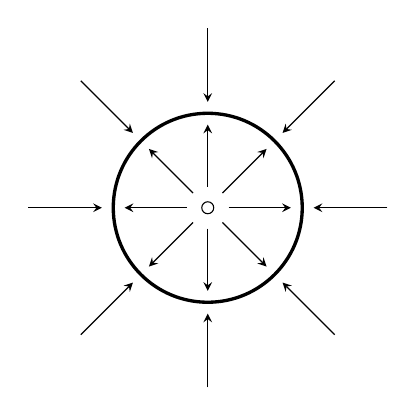
\begin{tikzpicture}[scale=1.2,>=stealth]
        \draw[very thick] (0,0) circle (1);
        \foreach \a in {0,45,...,315} {
            \draw[->] ({1.9*cos(\a)},{1.9*sin(\a)})--({1.12*cos(\a)},{1.12*sin(\a)});
            \draw[->] ({0.22*cos(\a)},{0.22*sin(\a)})--({0.88*cos(\a)},{0.88*sin(\a)});
        }
        \draw[fill=white] (0,0) circle (1.8pt);
    \end{tikzpicture}
    \caption{The punctured plane deformation retracts onto the circle by pushing every point along its ray.}
    \label{fig radial retraction}
\end{figure}

\begin{example}\label{example deformation retracts}
    \begin{enumerate}
        \item The punctured space $\bbR^n\setminus\{0\}$ deformation retracts onto the sphere $\bbS^{n-1}$ via $r_t(\bf{x})=(1-t)\bf{x}+t\frac{\bf{x}}{\lvert \bf{x}\rvert}$, pushing every point radially onto the unit sphere (Figure~\ref{fig radial retraction}). Similarly, the cylinder $\bbS^1\times\bbR$ deformation retracts onto the circle $\bbS^1\times\{0\}$.
        \item The M\"obius band, as the square $[0,1]^2$ with $(0,y)\sim(1,1-y)$, deformation retracts onto its core circle $y=\frac12$ via $r_t(x,y)=(x,(1-t)y+\frac t2)$. This homotopy is compatible with the gluing, because $(1-t)(1-y)+\frac t2=1-\big((1-t)y+\frac t2\big)$. So the M\"obius band, the cylinder and the circle are all homotopy equivalent, although no two of them are homeomorphic.
        \item The plane with two points removed deformation retracts onto a figure eight surrounding the two points, and also onto a theta-shaped graph $\ominus$. Thus $\bbS^1\vee\bbS^1\simeq\ominus$, even though they are not homeomorphic (Example~\ref{example cut points}).
        \item \emph{Gram-Schmidt.}\index{Gram-Schmidt process} Every invertible matrix can be uniquely written as $A=QR$, where $Q\in\Or_n$ and $R$ is upper triangular with positive diagonal entries, and $Q$ and $R$ depend continuously on $A$ by the explicit Gram-Schmidt formulas. The homotopy $r_t(A)=Q\big((1-t)R+t\rmI_n\big)$ stays in $\GL_n(\bbR)$, because such triangular matrices form a convex set. Therefore $\GL_n(\bbR)$ deformation retracts onto $\Or_n$, and similarly $\GL_n(\bbC)$ onto $\U_n$. All topological information about these large non-compact groups is contained in their compact subgroups.
    \end{enumerate}
\end{example}

The last examples suggest a way to recognize homotopy equivalent spaces: find a larger space of which both are deformation retracts. This always works.

\begin{defn}[Mapping cylinder]\index{Mapping cylinder}
    The \emph{mapping cylinder} of a map $f:X\to Y$ is the space $Z_f=\big((X\times[0,1])\sqcup Y\big)/\big((x,0)\sim f(x)\big)$, obtained by attaching the cylinder $X\times[0,1]$ to $Y$ along its end $X\times\{0\}$ via $f$ (Figure~\ref{fig mapping cylinder}).
\end{defn}

\begin{figure}[tp]
    \centering
    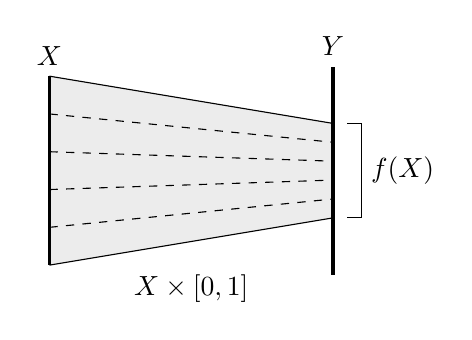
\begin{tikzpicture}[scale=1.2,>=stealth]
        \fill[gray!15] (0,-1)--(3,-0.5)--(3,0.5)--(0,1)--cycle;
        \draw (0,-1)--(3,-0.5) (0,1)--(3,0.5);
        \foreach \y in {-0.6,-0.2,0.2,0.6} { \draw[dashed] (0,\y)--(3,{\y/2}); }
        \draw[very thick] (0,-1)--(0,1) node[above]{$X$};
        \draw[very thick] (3,-1.1)--(3,1.1) node[above]{$Y$};
        \draw (3.15,0.5)--(3.3,0.5)--(3.3,-0.5)--(3.15,-0.5);
        \node[right] at (3.3,0) {$f(X)$};
        \node at (1.5,-1.25) {$X\times[0,1]$};
    \end{tikzpicture}
    \caption{The mapping cylinder of $f:X\to Y$. Each segment $\{x\}\times[0,1]$ (dashed) is attached to $Y$ at the point $f(x)$. Sliding along these segments deformation retracts $Z_f$ onto $Y$.}
    \label{fig mapping cylinder}
\end{figure}

The space $X$ embeds into $Z_f$ as the free end $X\times\{1\}$, and $Y$ is a deformation retract of $Z_f$: slide every point $(x,s)$ along its segment to $f(x)$, by $r_t(x,s)=(x,(1-t)s)$. The composition of the inclusion $X\hookrightarrow Z_f$ with the retraction $r_1:Z_f\to Y$ is $f$. So \emph{every map is an inclusion followed by a homotopy equivalence}. If both $X$ and $Y$ are deformation retracts of some space $Z$, then clearly $X\simeq Z\simeq Y$. Conversely, if $f$ is a homotopy equivalence, then $X$ is also a deformation retract of $Z_f$. This requires the homotopy extension property, and we will prove it in Corollary~\ref{cor 0.21 Hatcher}. Thus two spaces are homotopy equivalent iff they are (homeomorphic to) deformation retracts of a common space.


\subsection{Spheres and Brouwer's fixed point theorem}

Is the sphere $\bbS^n$ contractible? For $n=0$ the answer is no, since $\bbS^0$ consists of two points. For $n=1$, the circle is not contractible: in the next \sect\ we will see that its fundamental group is nontrivial (Theorem~\ref{thm pi1 of circle elementary}).

\begin{thm}\label{thm spheres not contractible}
    The sphere $\bbS^n$ is not contractible.
\end{thm}
\begin{proof}
    There is a plethora of different proofs of this theorem, from purely analytical to algebraic. An analytic proof, based on Sard's theorem, is given in Corollary~\ref{cor Brouwer smooth}. We will give another proof when we compute the homology groups of the spheres in \Part~\ref{Part Homology} and observe that they differ from those of a point.
\end{proof}

This seemingly obvious fact has a famous consequence.

\begin{thm}[Brouwer's fixed point theorem]\index{Theorem!Brouwer's fixed point}\label{thm Brouwer's fixed point}
    Every continuous map $f:\wb{B^n}\to\wb{B^n}$ of the closed unit ball to itself has a fixed point.
\end{thm}
\begin{proof}
    Suppose $f(\bf{x})\neq \bf{x}$ for all $\bf{x}$. Let $h(\bf{x})$ be the point where the ray from $f(\bf{x})$ through $\bf{x}$ leaves the ball (Figure~\ref{fig Brouwer}). Solving a quadratic equation for this point shows that $h$ is continuous, and $h(\bf{x})=\bf{x}$ for $\bf{x}\in\bbS^{n-1}$, so $h$ is a retraction of $\wb{B^n}$ onto its boundary sphere. Then $F(t,\bf{x})=h(t\bf{x})$, $\bf{x}\in\bbS^{n-1}$, is a homotopy from a constant map to $\id_{\bbS^{n-1}}$, so $\bbS^{n-1}$ is contractible. This contradicts Theorem~\ref{thm spheres not contractible} (for $n=1$, it contradicts the disconnectedness of $\bbS^0$).
\end{proof}

\begin{figure}[tp]
    \centering
    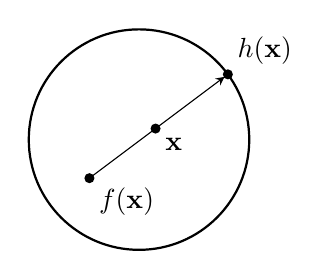
\begin{tikzpicture}[scale=1.4,>=stealth]
        \draw[thick] (0,0) circle (1);
        \fill (-0.45,-0.35) circle (1.3pt) node[below right]{$f(\bf{x})$};
        \fill (0.15,0.1) circle (1.3pt) node[below right]{$\bf{x}$};
        \draw[->,shorten >=1.5pt] (-0.45,-0.35)--(0.8059,0.5919);
        \fill (0.8059,0.5919) circle (1.3pt) node[above right]{$h(\bf{x})$};
    \end{tikzpicture}
    \caption{If $f$ had no fixed point, the ray from $f(\bf{x})$ through $\bf{x}$ would define a retraction $h$ of the ball onto its boundary sphere.}
    \label{fig Brouwer}
\end{figure}

\begin{rem}\label{rem Brouwer equivalent}
    The two theorems are in fact equivalent: conversely, a contraction of $\bbS^{n-1}$ would give a retraction of the ball onto its boundary, and composing with the antipodal map would produce a map of the ball without fixed points. For $n=2$, the proof is complete already by Corollary~\ref{cor no retraction D2 S1}. The general case is settled in Corollary~\ref{cor Brouwer smooth}.
\end{rem}

\begin{xca}
    Show that a map $f:\bbS^n\to\bbS^n$ without fixed points is homotopic to the antipodal map, and that a map without antipodal points ($f(\bf{x})\neq-\bf{x}$) is homotopic to the identity. \emph{Hint:} Example~\ref{example homotopies}.
\end{xca}
\begin{xca}
    Show that the \emph{cone}\index{Cone} $CX=([0,1]\times X)/(\{0\}\times X)$ over any space $X$ is contractible, and that a map $f:X\to Y$ is null-homotopic iff it extends to a map $CX\to Y$. For $X=\bbS^{n-1}$, the cone is the closed ball $\wb{B^n}$.
\end{xca}
\begin{xca}
    Show that $\bbR^3$ with a line removed is homotopy equivalent to $\bbS^1$, and that $\bbR^3$ with a point removed is homotopy equivalent to $\bbS^2$.
\end{xca}
\begin{xca}
    Show that $\SL_n(\bbR)$ deformation retracts onto $\SO_n$.
\end{xca}


\section{Fundamental group}\label{sec: fundamental group}

The invariant $\pi_0$ counts the pieces of a space by asking which points can be joined by paths. It cannot distinguish, say, the plane from the punctured plane. The difference between them is that a loop around the puncture cannot be shrunk to a point. So the next step is to ask which \emph{loops} can be deformed into each other.

\begin{defn}[Loops, Pointed homotopy]\index{Loop}
    Let $X$ be a path-connected topological space, pick a ``base point'' $x_0\in X$, and consider the set of all \emph{loops}\index{Homotopy!pointed} in $X$ based at $x_0$, i.e., paths $\gamma\in C([0,1], X)$ such that $\gamma(0)=\gamma(1)=x_0$. A pointed homotopy between two such loops is a homotopy $F\in C([0,1]\times[0,1],X)$ such that $F(\cdot,0)=F(\cdot,1)=x_0$. Pointed homotopy is an equivalence relation on the set of based loops.
\end{defn}

\begin{defn}[Fundamental/Poincar\'e group]\index{Fundamental group}
    The fundamental group $\pi_1(X,x_0)$ of a path-connected space $X$ with a base point $x_0$ is defined as the set $\{ [\gamma]\}$ of pointed homotopy classes of based loops with the inversion operation given by $[\gamma(t)]^{-1}=[\gamma(1-t)]$ and the multiplication operation 
    \[
    [\gamma_1(t)]\circ [\gamma_2(t)]=\left[ \begin{cases} \gamma_1(2t), & t\in[0,1/2], \\ \gamma_2(2t-1), & t\in(1/2,1] \end{cases}\right].
    \]
    The unit element is given by the equivalence class of the ``constant loop'' $\gamma(t)\equiv x_0$. If $X$ is not path-connected, then $\pi_1(X,x_0)$ is defined as the fundamental group of the path-connected component containing $x_0$.
\end{defn}

\begin{xca}
    Check that this definition is consistent, i.e., the homotopy classes on the right-hand sides don't depend on the choices of representatives of the classes on the left.
\end{xca}
\begin{defn}[Simple-connectedness]\index{Simply connected space}
    A path-connected space $X$ is called simply connected if its fundamental group is trivial, $\pi_1(X,x_0)=\{e\}$.
\end{defn}

\begin{xca}
Show that contractible spaces are simply connected.
\end{xca}

\begin{thm}\label{thm retraction pi1}
    If a space $X$ retracts onto a subspace $A$, then the homomorphism of fundamental groups $i_\ast:\pi_1(A,x_0)\to \pi_1(X,x_0)$ induced by the inclusion $i: A\hookrightarrow X$ is injective. If $A$ is a deformation retract of $X$, then $i_\ast$ is an isomorphism.
\end{thm}
\begin{proof}
    If $r:X\to A$ is a retraction then $r\circ i=\mathrm{id}_A$, hence by functoriality of $\pi_1$, $r_\ast \circ i_\ast=\mathrm{id}_{\pi_1(A,x_0)}$, which implies injectivity. If $r_t$ is a deformation retraction, then for any loop $\gamma$ in $X$ based at $x_0\in A$ the composition $r_t\circ \gamma$ gives a homotopy of $\gamma$ to a loop in $A$, therefore $i_\ast$ is also surjective.
\end{proof}

\begin{defn}[Alternative approach]
    Recall that the category $\mathsf{Top}_\bullet$ consists of ``pointed topological spaces'' with chosen basepoints and morphisms that are continuous maps mapping basepoint to basepoint. Take the circle $\bbS^1$ and pick a point $\bullet$ in it. Then one can redefine based loops as morphisms between two pointed topological spaces $\gamma\in C((\bbS^1,\bullet),(X,x_0))$. Pointed homotopy in the definition of $\pi_1$ can then be replaced by just homotopy of loops as maps defined on $\bbS^1$. Thus, as a set, $\pi_1(X)=[\bbS^1,X]_\bullet$ (group of homotopy classes of pointed maps).
\end{defn}

\begin{prop}\label{prop computing pi1}
\begin{enumerate}
    \item $\pi_1$ is a covariant functor $\pi_1:\mathsf{Top}_\bullet\to \mathsf{Gr}$.
    \item For a path-connected space, fundamental groups with different base points are isomorphic (this is why we often abuse the notation by writing $\pi_1(X)$).
    \item For any number of path-connected spaces, $\pi_1(\prod_\alpha X_\alpha)\cong \prod_\alpha \pi_1(X_\alpha)$.
\end{enumerate}
\end{prop}
\begin{proof}
Exercise.
\end{proof}

So far we have not computed a single nontrivial fundamental group. The simplest candidate is the circle, and the key to it is a very concrete object: the continuous choice of an angle. Let
\[p:\bbR\to\bbS^1\subset\bbC,\quad p(x)=\rme^{2\pi\rmi x},\]
so that $x$ measures the angle in full turns. Every point of $\bbS^1$ has infinitely many angles, differing by integers, and the whole difficulty is to choose them continuously along a path. Denote by $\mathrm{Arg}:\bbS^1\setminus\{-1\}\to(-\pi,\pi)$ the principal value of the argument; it is continuous, and $\rme^{\rmi\,\mathrm{Arg}(z)}=z$.

\begin{figure}[tp]
    \centering
    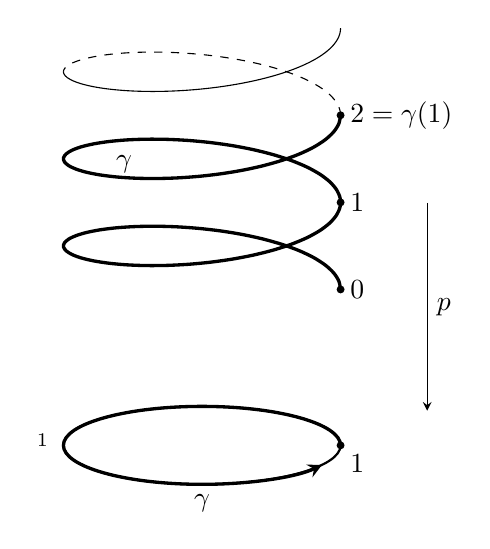
\begin{tikzpicture}[scale=1.1,>=stealth]
        % base circle
        \draw[thick] (0,-1.8) ellipse (1.6 and 0.45);
        \node[left] at (-1.65,-1.8) {$\bbS^1$};
        \fill (1.6,-1.8) circle (1.3pt) node[below right] {$1$};
        % helix (back parts dashed)
        \foreach \k in {0,1,2} {
            \draw[thin, domain={2*pi*\k}:{2*pi*\k+pi}, samples=40, smooth, variable=\t, dashed]
                plot ({1.6*cos(\t r)}, {0.45*sin(\t r)+0.16*\t});
            \draw[thin, domain={2*pi*\k+pi}:{2*pi*(\k+1)}, samples=40, smooth, variable=\t]
                plot ({1.6*cos(\t r)}, {0.45*sin(\t r)+0.16*\t});
        }
        \node[left] at (-1.6,2.6) {$\bbR$};
        % lifted path from 0 to 2
        \draw[very thick, domain=0:{4*pi}, samples=80, smooth, variable=\t]
            plot ({1.6*cos(\t r)}, {0.45*sin(\t r)+0.16*\t});
        \foreach \k/\h in {0/0, 1/1.005, 2/2.011} {
            \fill (1.6,\h) circle (1.3pt);
        }
        \node[right] at (1.6,0) {$0$};
        \node[right] at (1.6,1.005) {$1$};
        \node[right] at (1.6,2.011) {$2=\wt\gamma(1)$};
        \node at (-0.9,1.45) {$\wt\gamma$};
        % projection
        \draw[->] (2.6,1) -- node[right] {$p$} (2.6,-1.4);
        % loop downstairs
        \draw[very thick, ->] (1.6,-1.8) arc (0:330:1.6 and 0.45);
        \node[below] at (0,-2.25) {$\gamma$};
    \end{tikzpicture}
    \caption{The exponential map $p(x)=\rme^{2\pi\rmi x}$ wraps $\bbR$ around $\bbS^1$ like a spring. A loop $\gamma$ going twice around the circle lifts to a path climbing from $0$ to $2$.}
    \label{fig: lifting to R}
\end{figure}

\begin{lem}[Continuous choice of angle]\label{lem lifting to R}
\begin{enumerate}
    \item For every path $\gamma:[0,1]\to\bbS^1$ and every $x_0\in\bbR$ with $p(x_0)=\gamma(0)$ there is a unique continuous \emph{lift}\index{Lift of a path} $\wt\gamma:[0,1]\to \bbR$ with $p\circ\wt\gamma=\gamma$ and $\wt\gamma(0)=x_0$.
    \item For every continuous map $H:[0,1]\times[0,1]\to\bbS^1$ and every $x_0$ with $p(x_0)=H(0,0)$ there is a unique continuous lift $\wt H:[0,1]\times[0,1]\to\bbR$ with $p\circ\wt H=H$ and $\wt H(0,0)=x_0$.
\end{enumerate}
\end{lem}
\begin{proof}
    \emph{Uniqueness.} Two lifts of the same map differ by a continuous function with values in $\bbZ$ (since $p(x)=p(y)$ iff $x-y\in\bbZ$). On a connected domain such a function is constant, and it vanishes at the starting point.

    \emph{Existence in (1).} By uniform continuity of $\gamma$ on the compact interval (Proposition~\ref{prop uniform continuity}), there is $N$ such that $\gamma$ moves by less than half a turn on each interval $[t_k,t_{k+1}]$, $t_k=k/N$; that is, $\gamma(t)/\gamma(t_k)\neq -1$ there. Then we simply add up small angle increments: define $\wt\gamma(0)=x_0$ and, inductively in $k$,
    \[\wt\gamma(t)=\wt\gamma(t_k)+\frac{1}{2\pi}\mathrm{Arg}\frac{\gamma(t)}{\gamma(t_k)},\qquad t\in[t_k,t_{k+1}].\]
    Each piece is continuous, and consecutive pieces agree at $t_k$. Moreover, we have $p(\wt\gamma(t))=p(\wt\gamma(t_k))\cdot\gamma(t)/\gamma(t_k)=\gamma(t)$.

    \emph{Existence in (2).} First lift the path $t\mapsto H(t,0)$ by (1) to get $\wt H(t,0)$. By uniform continuity of $H$ on the compact square, there is $N$ such that $H(t,s)/H(t,s_k)\neq -1$ for all $t$ and all $s\in[s_k,s_{k+1}]$, $s_k=k/N$. Now apply the same formula in the variable $s$:
    \[\wt H(t,s)=\wt H(t,s_k)+\frac{1}{2\pi}\mathrm{Arg}\frac{H(t,s)}{H(t,s_k)},\qquad s\in[s_k,s_{k+1}].\]
    By induction in $k$, each step is a continuous function of \emph{both} variables $(t,s)$.
\end{proof}

\begin{defn}[Degree of a loop]\index{Degree!of a loop in $\bbS^1$}\index{Winding number}
    The \emph{degree} (or \emph{winding number}) of a closed path $\gamma:[0,1]\to\bbS^1$, $\gamma(0)=\gamma(1)$, is the integer
    \[\deg\gamma=\wt\gamma(1)-\wt\gamma(0)\in\bbZ,\]
    where $\wt\gamma$ is any lift of $\gamma$. It does not depend on the choice of the lift, since any two lifts differ by a constant.
\end{defn}

\begin{prop}\label{prop degree homotopy invariant}
    If $H:[0,1]\times[0,1]\to\bbS^1$ is a homotopy through closed paths (i.e., $H(t,0)=H(t,1)$ for all $t$; the basepoint is allowed to move), then $\deg H(0,\cdot)=\deg H(1,\cdot)$.
\end{prop}
\begin{proof}
    Take the lift $\wt H$ from Lemma~\ref{lem lifting to R}. By uniqueness, $\wt H(t,\cdot)$ is a lift of $H(t,\cdot)$ for every $t$, so $\deg H(t,\cdot)=\wt H(t,1)-\wt H(t,0)$ is a continuous integer-valued function of $t\in[0,1]$, hence constant.
\end{proof}

\begin{thm}[Fundamental group of the circle]\label{thm pi1 of circle elementary}
    The degree defines an isomorphism $\deg:\pi_1(\bbS^1,1)\to\bbZ$. The class of the loop $\omega_n(s)=\rme^{2\pi\rmi ns}$ corresponds to $n$.
\end{thm}
\begin{proof}
    By Proposition~\ref{prop degree homotopy invariant}, $\deg$ is well defined on homotopy classes.

    \emph{Homomorphism.} Let $\wt\beta,\wt\gamma$ be lifts of $\beta,\gamma$ starting at $0$. Then $\wt\beta$ followed by the shifted path $\wt\gamma+\deg\beta$ is a lift of the concatenation $\beta\bullet\gamma$ (first $\beta$, then $\gamma$), which represents $[\beta]\circ[\gamma]$, and it ends at $\deg\beta+\deg\gamma$.

    \emph{Surjectivity.} The loop $\omega_n$ lifts to $s\mapsto ns$, so $\deg\omega_n=n$.

    \emph{Injectivity.} If $\deg\gamma=0$, the lift $\wt\gamma$ starting at $0$ ends at $0$, i.e., it is a loop in $\bbR$. Shrinking it linearly, $F(t,s)=p\big((1-t)\wt\gamma(s)\big)$ is a pointed homotopy from $\gamma$ to the constant loop.
\end{proof}

\begin{rem}
    The map $p$ is the prototype of a \emph{covering map}, and Lemma~\ref{lem lifting to R} is a special case of the path and homotopy lifting properties, Theorems~\ref{Path lifting property} and \ref{homotopy lifting property}. In the \chap\ on covering spaces, the same computation will reappear as Theorem~\ref{pi_1 of the circle thm}, this time as a consequence of the general theory.
\end{rem}

The circle is therefore not simply connected, and in particular not contractible. This single computation already has striking consequences.

\begin{cor}[No retraction]\label{cor no retraction D2 S1}
    There is no retraction of the closed disk $\wb{B^2}$ onto its boundary circle $\bbS^1$. Consequently, Brouwer's fixed point theorem (Theorem~\ref{thm Brouwer's fixed point}) holds for $n=2$.
\end{cor}
\begin{proof}
    By Theorem~\ref{thm retraction pi1}, a retraction would make $i_\ast:\pi_1(\bbS^1)\cong\bbZ\to \pi_1(\wb{B^2})=0$ injective, which is absurd. The proof of Brouwer's theorem constructs exactly such a retraction $h$ from a map without fixed points.
\end{proof}

\begin{cor}[Fundamental theorem of algebra]\index{Theorem!Fundamental theorem of algebra}\label{cor FTA}
    Every polynomial $P(z)=z^n+a_{n-1}z^{n-1}+\dots+a_0$ with complex coefficients and $n\geq1$ has a complex root.
\end{cor}
\begin{proof}
    Suppose $P$ has no roots. Then for every $r\geq0$, we get a closed path in $\bbS^1$:
    \[\gamma_r(s)=\frac{P(r\rme^{2\pi\rmi s})}{\lvert P(r\rme^{2\pi\rmi s})\rvert},\]
    and $r\mapsto\gamma_r$ is a homotopy through closed paths. For $r=0$ the path is constant, so $\deg\gamma_r=0$ for all $r$ by Proposition~\ref{prop degree homotopy invariant}.

    On the other hand, take $R>1+\sum_k\lvert a_k\rvert$. On the circle $\lvert z\rvert=R$ we have $\lvert z^n\rvert>\lvert a_{n-1}z^{n-1}+\dots+a_0\rvert$, so the polynomials $P_t(z)=z^n+t(a_{n-1}z^{n-1}+\dots+a_0)$, $t\in[0,1]$, have no zeros there. Normalizing $P_t(R\rme^{2\pi\rmi s})$ as before gives a homotopy through closed paths from $\gamma_R$ to $s\mapsto \rme^{2\pi\rmi ns}=\omega_n$, whose degree is $n\neq0$. Contradiction.
\end{proof}

\begin{lem}\label{lem product of loops}\index{Product of loops}
    If a space $X$ is the union of a collection of path-connected open sets $U_\alpha$ each containing the basepoint $x_0$ and if each intersection $U_{\alpha\beta}$ is path-connected, then every loop in $X$ at $x_0$ is homotopic to a product of loops each of which is contained in a single $U_\alpha$.
\end{lem}
\begin{proof}
    The key is in the compactness of the interval $[0,1]$, which guarantees that the loop can be broken up into a finite number of segments each of which is contained inside a single $U_{\alpha_i}$. Call these segments $f_i$, $i=1,\ldots,n$. The starting point of $f_i$ ($i\geq 2$) lies in $U_{\alpha_{i-1}}\cap U_{\alpha_i}$, which is path-connected and contains $x_0$, so we can find a path $g_i$ inside this intersection from $x_0$ to the starting point of $f_i$. We choose $g_1$ and $g_{n+1}$ to be trivial. The loops we seek are then $g_i\cdot f_i\cdot g_{i+1}^{-1}$, each lying in $U_{\alpha_i}$. Their product is homotopic to the original loop because all $g_i$'s cancel out.
\end{proof}
\begin{cor}\label{cor pi_1(S^n)=0}
    $\pi_1(\bbS^n)=0$ for $n\geq 2$.
\end{cor}
\begin{proof}
    $\bbS^n$ is the union of the open neighborhoods of two hemispheres, $U_+$ and $U_-$. Each of these is homeomorphic to $\bbR^n$ and $U_+\cap U_-\cong \bbS^{n-1}\times \bbR $. If $n\geq 2$, then $U_+\cap U_-$ is path-connected. By the above lemma, every loop in $\bbS^n$ based at a point $x_0\in U_+\cap U_-$ is homotopic to a product of loops each lying in one of $U_\pm$. However all of these loops are trivial since $\pi_1(U_\pm)=0$.
\end{proof}
\begin{cor}
    $\bbR^2$ is not homeomorphic to $\bbR^n$ for $n\neq 2$.
\end{cor}
\begin{proof}
    Assume there is a homeomorphism $f:\bbR^2\to \bbR^n$. The case $n=1$ is easy because $\bbR \setminus\{f(0)\}$ is not connected whereas the supposedly homeomorphic $\bbR^2\setminus\{0\}$ is. When $n>2$, $f$ restricts to a homeomorphism $\bbR^2\setminus\{0\}\to\bbR^n\setminus\{f(0)\}$. Each of these punctured spaces deformation retracts onto a sphere around the removed point (via $\bf{x}\mapsto \bf{x}/\lvert \bf{x}\rvert$), so their fundamental groups are $\pi_1(\bbS^1)\cong\bbZ$ (Theorem~\ref{thm pi1 of circle elementary}) and $\pi_1(\bbS^{n-1})=0$ (Corollary~\ref{cor pi_1(S^n)=0}), respectively. This is a contradiction.
\end{proof}

We are now prepared to prove one of the most important theorems about the fundamental group. First let us recall the categorical notion of pushouts (see Definition~\ref{pushouts}). If a path-connected space is represented as a union of two open sets, $X=U\cup V$, then the corresponding set inclusions induce homomorphisms of fundamental groups:
\[
    \begin{tikzcd}[every matrix/.append style={name=m},   
    execute at end picture={\draw [<-] ([xshift=-8.5mm,yshift=1mm]m-2-2.north) arc[start angle=-90,delta angle=270,radius=0.25cm];}]
    X \arrow[r,leftarrow,"l"]\arrow[d,leftarrow,"k"]& V\arrow[d,leftarrow,"j"] \\
    U\arrow[r,,leftarrow,swap,"i"]& U\cap V\\
    \end{tikzcd}
    \quad\quad\quad\quad\quad
    \begin{tikzcd}[every matrix/.append style={name=m},   
    execute at end picture={\draw [<-] ([xshift=-11.5mm,yshift=1mm]m-2-2.north) arc[start angle=-90,delta angle=270,radius=0.25cm];}]
    \pi_1(X) \arrow[r,leftarrow,"l_\ast"]\arrow[d,leftarrow,"k_\ast"]& \pi_1(V)\arrow[d,leftarrow,"j_\ast"] \\
    \pi_1(U)\arrow[r,,leftarrow,swap,"i_\ast"]& \pi_1(U\cap V)\\
    \end{tikzcd}
\]
$X$ itself is in fact the pushout, $X=U\sqcup_{U\cap V}V$. \emph{The Seifert-van~Kampen theorem will show that the functor $\pi_1$ preserves pushouts,} i.e., the fundamental group of the union is isomorphic to the amalgamated free product, $\pi_1(X)\cong \pi_1(U) \ast_{\pi_1(U\cap V)} \pi_1(V)$. By the universal property of the free product, there is a unique homomorphism $\varPhi$ in the diagram below that makes the external triangles commute.
\[
    \begin{tikzcd}
    \pi_1(U)\ast \pi_1(V)   \arrow[drr,leftarrow, bend left]   \arrow[ddr,leftarrow, bend right]   \arrow[dr,"\exists! \varPhi" description] & & \\
        & \pi_1(X) \arrow[r,leftarrow,swap, "l_\ast"] \arrow[d,leftarrow, "k_\ast"]       & \pi_1(V) \arrow[d,leftarrow, "j_\ast"] \\ & \pi_1(U) \arrow[r,leftarrow,swap, "i_\ast"] &\pi_1(U\cap V) 
    \end{tikzcd}
\]
Note, however, that the ``background square'' involving $\pi_1(U\cap V),\pi_1(U),\pi_1(V)$, and $\pi_1(U)\ast \pi_1(V)$ \emph{does not commute}, so the universal property of the pushout \emph{will not} apply in the other direction to give a homomorphism $\pi_1(X)\to \pi_1(U)\ast\pi_1(V)$. Instead, we will compute $\pi_1(X)$ by finding the kernel of $\varPhi$ and factoring it out.

\begin{thm}[Seifert-van Kampen {{\cite[Thm.~1.20]{Hatcher}}}]\index{Theorem!Seifert-van~Kampen}\label{thm seifert-van kampen}
    If $X$ is the union of path-connected open sets $U_\alpha$ each containing the basepoint $x_0\in X$ and if each intersection $U_{\alpha\beta}$ is path-connected, then the homomorphism $\varPhi: \ast_\alpha \pi_1(U_\alpha)\to \pi_1(X)$ induced by the inclusions $U_\alpha \hookrightarrow X$ is surjective. 

    Denote the inclusion-induced homomorphisms $i_\alpha:\pi_1(U_\alpha)\to \pi_1(X)$ and $i_{\alpha\beta}:\pi_1(U_{\alpha\beta})\to \pi_1(U_\alpha)$. We have $i_\alpha \circ i_{\alpha\beta}=i_{\beta}\circ i_{\beta\alpha}$ since both sides are induced by the inclusion $U_{\alpha\beta}\hookrightarrow X$. Now, if in addition each intersection $U_{\alpha\beta\gamma}$ is path-connected, then the kernel of $\varPhi$ is the normal subgroup $N$ generated by all elements of the form $i_{\alpha\beta }(g)i_{\beta\alpha}(g)^{-1}$ for $g\in\pi_1(U_{\alpha\beta})$, and hence $\varPhi$ induces an isomorphism $\pi_1(X)\cong \ast_\alpha \pi_1(U_\alpha)/N$.

    In particular, in the case of two sets, $\pi_1(U\cup V)\cong \pi_1(U)\ast_{\pi_1(U\cap V)}\pi_1(V)$.
\end{thm}
\begin{proof}
    The surjectivity of $\varPhi$ was already shown in Lemma~\ref{lem product of loops}. 

    Now we need to show that the kernel of $\varPhi$ is exactly $N$. We already know that $N\subset \ker \varPhi$ since $i_\alpha\circ i_{\alpha\beta}=i_\beta\circ i_{\beta\alpha}$. For the reverse inclusion, the idea is to study \emph{factorizations} of loops into ``smaller'' loops $[\gamma_i]$ that are completely contained in one of the $U_\alpha$'s. There are two ``moves'' that, as we would like to show, transform differing factorizations of the same loop into each other. Namely, a substring of the form $[\gamma_i][\gamma_{i+1}]$ can be replaced with $[\gamma_i\cdot \gamma_{i+1}]$, and an element $[\gamma_i]$ viewed as an element of $\pi_1(U_\alpha)$ can be replaced with its analog in $\pi_1(U_\beta)$ if $\gamma_i$ is a loop contained in $U_{\alpha\beta}$. If we can show that all factorizations of a loop can be transformed into each other via a sequence of moves of this kind (or their inverses), that will mean that $\varPhi$ induces an \emph{injective} map from the quotient group into $\pi_1(X)$, and thus the kernel of $\varPhi$ is exactly $N$.

    The goal is therefore to decompose any homotopy of loops into a sequence of moves like this. A homotopy is a continuous map defined on the unit square, $H:[0,1]\times[0,1]\to X$, whose value on the left and right edges of the square is $x_0$. Now we need to subdivide this square into smaller squares as in the Figure, so that each square is mapped entirely into only one of the open sets $U_\alpha$, and so that the resulting subdivisions of the top and bottom edges of the square are refinements of the subdivisions implied in the two factorizations at hand (that is, each interval of the new subdivision is entirely contained in an interval from the old). Lastly, we can ``perturb'' the squares in the central rows so that each point is contained in at most three squares (this is why triple intersections were required to be path-connected).

    \begin{center}
        \includegraphics[scale=0.75]{figures/subdivision.pdf}
    \end{center}

    Now we proceed to define a sequence of paths along the edges of the subdivision from the left to the right side of the square that progressively ``capture'' more and more of the squares. For each segment we need to specify which of the open sets in $X$ its image is supposed to belong to, which is exactly the second move (in other words, $i_{\alpha\beta\ast}([\gamma_i])$ and $i_{\beta\alpha\ast}([\gamma_i])$ belong to the same coset in the quotient group). Further, each successive path is homotopic to the last via a deformation of a loop inside one $U_\alpha$. All together, this proves that any two factorizations of the same loop are equivalent in the sense that they differ only by relations that define the group $N$. The illustration below is from \cite[Chapter 10]{LeeTop}.

    \begin{center}
        \includegraphics[scale=1]{figures/kernel of Phi.pdf}
    \end{center}

    See \cite[Thm.~1.20]{Hatcher} for more details of the proof.
\end{proof}

The conditions on path-connectedness of intersections and on the basepoint seem artificial, and indeed they are. Any open covering of $X$ can be turned into a covering of this kind by taking unions of sets lying along paths connecting them to the original basepoint. The full version of the Seifert-van~Kampen theorem can be stated purely in categorical terms with no extra conditions, however first we will need the notion of the \emph{fundamental groupoid}.

\begin{defn}[Groupoid]\index{Groupoid}
    A groupoid is a set with a unary ``inversion'' map $x\mapsto x^{-1}$ and a partial (i.e., not necessarily defined for any pair of elements) associative binary ``multiplication'' operation $(x,y)\mapsto x\bullet y$. It is associative in the sense that if both $x\bullet y$ and $y\bullet z$ exist, then both $(x\bullet y)\bullet z$ and $x\bullet (y\bullet z)$ exist and coincide. It is also required that $x\bullet x^{-1}$ and $x^{-1}\bullet x$ exist, and that, if $x\bullet y$ exists, then $x\bullet y\bullet y^{-1}=x$ and $x^{-1}\bullet x\bullet y=y$.

   As a consequence of these axioms, $(x^{-1})^{-1}=x$ and $(x\bullet y)^{-1}=y^{-1}\bullet x^{-1}$. Intuitively, groupoids can be thought of as groups with many identities, where $x\bullet y$ is defined only when the ``right identity'' of $x$ matches the ``left identity'' of $y$, i.e., $x^{-1}\bullet x=y\bullet y^{-1}$. 

    An equivalent definition is that a groupoid is a category where all morphisms are invertible (i.e., isomorphisms). The objects of this category are the ``identities'' of the groupoid. A group is then simply a groupoid with a single object. The category of groupoids is denoted $\mathsf{Grpd}$.
\end{defn}

Free products of groupoids can be constructed in the same way as for groups -- as strings of ``words'' $g_1^{\epsilon_1} \cdots g_n^{\epsilon_n}$ where each product $g_i^{\epsilon_i}\bullet g_{i+1}^{\epsilon_{i+1}}$ must exist and insertions of substrings of the form $gg^{-1}$ produce an equivalent string. These free products have the same universal property, i.e., they are the coproducts in $\mathsf{Grpd}$; pushouts are obtained from them by imposing further relations.

\begin{defn}[Fundamental groupoid]\index{Fundamental groupoid}
    Given a topological space $X$, let $\Pi(X)$ (also denoted $\Pi_1(X)$) be the category whose objects are points of $X$ and the morphisms $\mathrm{Mor}(x,y)$ are the homotopy classes (relative to the endpoints) of paths $\gamma:[0,1]\to X$ such that $\gamma(0)=x, \gamma(1)=y$. Since continuous images of homotopic paths are homotopic, we have a functor $\Pi:\mathsf{Top}\to \mathsf{Grpd}$.
\end{defn}
Notice that the set of endomorphisms of any $x\in X$ viewed as an object in $\Pi(X)$ is exactly the group $\pi_1(X,x)$. Moreover, it's not difficult to check that homotopies of continuous maps in $\mathsf{Top}$ induce natural transformations of the corresponding $\Pi$-functors.
\begin{prop}
    For a path-connected space $X$, the inclusion $\pi_1(X,x)\hookrightarrow \Pi(X)$ is an equivalence of categories.
\end{prop}
\begin{proof}
    Indeed, viewed as a category with a single object, $\pi_1(X,x)$ forms a skeleton of $\Pi(X)$, since all objects of $\Pi(X)$ are isomorphic due to path-connectedness.
\end{proof}

\begin{thm}[Seifert-van~Kampen]\index{Theorem!Seifert-van~Kampen}
    Let $\mathscr{U}=\{U_\alpha\}_\alpha$ be an open covering of a space $X$ that is closed under finite intersections. Regard $\mathscr{U}$ as an index category whose morphisms are the inclusions of sets. The functor $\Pi$, restricted to sets and maps in $\mathscr{U}$, produces a diagram of groupoids $\Pi(\mathscr{U})$, i.e.
    \[\restr{\Pi}{\mathscr{U}}: \mathscr{U}\to \mathsf{Grpd}.\]
    Then the groupoid $\Pi(X)$ is the colimit (or pushout) of this diagram (that is, the initial object in the category of cones over $\restr{\Pi}{\mathscr{U}}$, see \S\ref{Limits and colimits}).
\end{thm}
\begin{proof}
    We can verify the universal property. For a groupoid $G$ and a set of groupoid homomorphisms $\eta_\alpha:\Pi(U_\alpha)\to G$ (forming a cone over $\restr{\Pi}{\mathscr{U}}$), we must construct a groupoid homomorphism $\wt{\eta}:\Pi(X)\to G$ (which is nothing but a functor between categories) that restricts to $\eta_\alpha$ on $\Pi(U_\alpha)$ for all $\alpha$. On objects, that is on points of $X$, we have no choice but to define $\wt{\eta}(x)=\eta_\alpha(x)$ for $x\in U_\alpha$. This is independent of the choice of $\alpha$ since the cover is closed under finite intersections.

    Now we must define $\wt{\eta}$ on morphisms in $\Pi(X)$, i.e., paths. If a path $\gamma$ connecting $x$ to $y$ lies entirely in a particular $U_\alpha$, we again have only one choice: $\wt{\eta}([\gamma])=\eta_\alpha([\gamma])$. This is consistent (independent of $\alpha$) since $\mathscr{U}$ is closed under finite intersections.

    Now, any path $\gamma$ is the composite of finitely many paths $\gamma_i$, each of which lies in a single $U_{\alpha_i}$. Therefore we must define $\wt{\eta}([\gamma])=\wt{\eta}([\gamma_1])\bullet \cdots \bullet \wt{\eta}([\gamma_n])$. 

    Clearly this definition will give the required unique morphism $\wt{\eta}$, provided that it is indeed well defined, i.e., respects the equivalence relation between paths. Thus suppose we have two equivalent paths $\gamma_0\sim \gamma_1$. The equivalence is given by a homotopy $\gamma_t$ through paths with the same fixed endpoints. This homotopy is a map defined on the square $[0,1]\times[0,1]$. We may subdivide the square into subsquares, each of which is mapped entirely into one of the $U_\alpha$'s. We may further choose this subdivision so that the resulting subdivision of $[0,1]\times\{0\}$ refines the subdivision used to decompose $\gamma_0$ into segments as above, and similarly for $\gamma_1$ and the resulting decomposition of $[0,1]\times \{1\}$. We see that the relation $[\gamma_0]=[\gamma_1]$ in $\Pi(X)$ is a consequence of a finite number of relations, each of which holds in one of the $\Pi(U_\alpha)$'s. Therefore $\wt{\eta}([\gamma_0])=\wt{\eta}([\gamma_1])$. This confirms that $\wt{\eta}$ is well defined and satisfies the universal property for pushouts.    
\end{proof}
From this, one can use an ``abstract nonsense'' argument to re-derive the original version of the theorem for the functor $\pi_1(-,x_0)$, see~\cite[\S 2.7]{May}.

The following is a straightforward consequence of the Seifert-van~Kampen Theorem in the ``limit'' where the overlap between the sets turns into a single point. We omit the proof.

\begin{cor}[Fundamental group of a wedge sum {{\cite[Thm.~10.7]{LeeTop}}}]
    Suppose $x_\alpha$ is a \emph{nondegenerate basepoint}\index{Nondegenerate basepoint} for $X_\alpha$ (i.e., $x_\alpha$ has a neighborhood which admits a strong deformation retraction onto $x_\alpha$). Then the basepoint of $\bigvee_{\alpha }X_\alpha$ is nondegenerate and the fundamental group of this wedge sum is isomorphic to the free product $\ast_{\alpha}\pi_1(X_\alpha)$.
\end{cor}

\begin{example}
\begin{enumerate}
    \item The shape $\ominus$ and the figure 8 (which is just the wedge sum $\bbS^1\vee \bbS^1$) are both deformation retracts of the plane with two points removed (Example~\ref{example deformation retracts}), so their fundamental groups are all $\bbZ\ast\bbZ$. Note that neither of the two shapes is homeomorphic to a subspace of the other: 8 has a point where four arcs meet, while $\ominus$ has two points where three arcs meet. Instead, $\ominus\to 8$ is the quotient map that collapses the middle bar to a point.
    \item The last example can be generalized to compute $\pi_1$ of an arbitrary connected graph. The result is just the free group generated by the set of ``elementary'' cycles in the graph. More precisely, the number of generators equals the number of all edges of the graph minus the number of edges in a maximal spanning tree of the graph (i.e., a maximal subgraph without cycles).
\end{enumerate}
\end{example}

\begin{xca}[{{\cite[Exercise 10-1]{LeeTop}}}]
    Use the Seifert-van~Kampen theorem to give another proof that $\bbS^n$ is simply connected when $n \geq 2$.
\end{xca}
\begin{xca}[{{\cite[Exercise 10-5]{LeeTop}}}]
    Compute the fundamental group of $\bbR^3$ with the three coordinate axes removed. \emph{Hint:} this space is homotopy equivalent to the 2-sphere with six points removed.
\end{xca}
\begin{xca}[Projective plane]\index{Projective plane}\label{RP2 exercise}
    Show that the projective plane $\RP^2$, constructed out of a disk by identifying the antipodal points on the bounding circle (see Figure~\ref{fig:crosscap}), has the fundamental group $\bbZ_2$.
\end{xca}
\begin{xca}[Crosscap]\index{Crosscap}\label{crosscap exercise}
    Show that the projective plane with a hole (also known as a \emph{crosscap}), constructed out of an annulus by identifying the antipodal points of the outer boundary, is homeomorphic to the M\"obius band, and therefore has fundamental group $\bbZ$.
\end{xca}
\begin{figure}[tp]
    \centering
    \includegraphics[scale=0.6]{figures/crosscap.pdf}
    \caption{Construction of the projective plane out of a disk. Adding a hole to this surface creates a crosscap, which is homeomorphic to a M\"obius band, see Exercises~\ref{RP2 exercise} and \ref{crosscap exercise}.}
    \label{fig:crosscap}
\end{figure}
\begin{xca}[{{\cite[Exercise III.3]{Bredon}}}]
    Consider an annulus. Identify antipodal points on the outer circle. Also identify antipodal points on the inner circle. Calculate the fundamental group of this surface. Is it homeomorphic to any of the orientable compact surfaces? \emph{Hint:} taking $U$ and $V$ to be overlapping annular neighborhoods of the two boundaries of the annulus, the generator of $\pi_1(U\cap V)$ is mapped to the square of the generator in $\pi_1(U)$ and similarly in $\pi_1(V)$; therefore $\pi_1(U\cup V)=\langle a,b\mid a^2=b^2\rangle$.
\end{xca}
\begin{xca}[{{\cite[Exercise 1.20]{Hatcher}}}]
    Let $X$ be the subspace of $\bbR^2$ that is the union of the circles $C_n$ of radius $n$ and center $(n, 0)$ for $n = 1, 2, \ldots$. Show that $\pi_1( X )$ is the free group $\ast_n \pi_1( C_n )$, the same as for the infinite wedge sum $\bigvee_{i=1}^\infty \bbS^1$. Show that $X$ and $\bigvee_{i=1}^\infty \bbS^1$ are in fact homotopy equivalent, but not homeomorphic.
\end{xca}

\begin{example}[Hawaiian earring {{\cite[Example~1.25]{Hatcher}}}]\label{hawaiian earring}
    Let $X$ be the subspace of $\bbR^2$ that is the union of the circles $C_n$ of radius $1/n$ and center $(1/n, 0)$ for $n = 1, 2, \ldots$. Initially this space can be mistaken for the infinite wedge sum $\bigvee_{i=1}^\infty \bbS^1$, but in fact it has a much larger fundamental group. This is because in the topology induced from $\bbR^2$ it is possible for a continuous loop $\gamma:[0,1]\to X$ to cover an infinite number of circles $C_n$ at once, unlike in the case of the wedge sum. As a result, $\pi_1(X)$ can be mapped surjectively onto the infinite direct product group $\prod_{n=1}^\infty \bbZ$, which is uncountably large. 
\end{example}

\begin{example}[Torus knots {{\cite[Example~1.24]{Hatcher}}}]
    For relatively prime integers $m,n$, the \emph{torus knot}\index{Torus knots}\index{Knot!torus} $K=K_{m,n}\subset \bbR^3$ is the image of the embedding $f:\bbS^1\to \bbS^1\times \bbS^1\cong \bbT^2\subset\bbR^3$ given by $f(z)=(z^m,z^n)$ ($z=\rme^{2\rmi\pi t}$), where the torus $\bbT^2$ is embedded in space in the standard way. Let us compute $\pi_1(\bbR^3\setminus K)$. First, we can safely replace $\bbR^3$ with its one-point compactification $\bbS^3$ (Example~\ref{example one point compactification}), because the Seifert-van~Kampen theorem shows that $\pi_1(\bbR^3\setminus K)\cong\pi_1(\bbS^3\setminus K)$. Now we may decompose $\bbS^3\setminus \bbT^2$ into two open solid tori $U,V$. Let $C$ be an open tubular neighborhood of $\bbT^2\setminus K$. Then $U\cup C$ and $V\cup C$ form an open covering of $\bbS^3\setminus K$ with a path-connected intersection. The fundamental groups of $U\cup C$, $V\cup C$, and the intersection $C$ are all isomorphic to $\bbZ$ and generated by loops $x,y,z$, respectively. The inclusions of $C$ into $V\cup C$ or $U\cup C$ map $z$ to $x^m$ or $y^n$. Therefore $\pi_1(\bbS^3\setminus K)=\langle x,y\mid x^m=y^n\rangle$. The center of this group is the subgroup generated by the element $x^m=y^n$, and the factor by the center is exactly $\bbZ_m\ast\bbZ_n$. By commuting all powers of $x^m$ through to the left, the elements of this group can be uniquely represented by strings of the form $x^{mk}w$, where $k\in\bbZ$ and $w$ is an alternating word $\cdots x^{k_1}y^{l_1}x^{k_2}y^{l_2}\cdots$ (possibly empty, and starting and ending with either letter) with $k_i\in\{1,\ldots,m-1\}$ and $l_i\in\{1,\ldots,n-1\}$.
\end{example}

\begin{example}[Lens spaces {{\cite[Exercise III.10]{Bredon}}}]\label{example Lens space bredon}
    Let $X=(\bbD^2\times \bbS^1)\sqcup_f (\bbD^2\times \bbS^1)$ be the gluing of two solid tori $V_1,V_2$ along a homeomorphism $f:\partial V_1\to\partial V_2$ of their boundary tori, induced from the linear map $\bbR^2\to\bbR^2$ given by an integer matrix $\begin{pmatrix}a&b\\c&d\end{pmatrix}$ with $ad-bc=\pm1$. On each boundary torus let $\alpha$ be the \emph{longitude} $\{\mathrm{pt}\}\times\bbS^1$ and $\beta$ the \emph{meridian} $\partial\bbD^2\times\{\mathrm{pt}\}$, and use the convention that the columns of the matrix are the images of $\alpha$ and $\beta$: $f_\ast\alpha=a\alpha+c\beta$, $f_\ast\beta=b\alpha+d\beta$. The fundamental group of $V_i$ is generated by its core circle $\gamma_i$, so that $\alpha\mapsto\gamma_i$ and $\beta\mapsto e$ under the inclusion of $\partial V_i$; the two solid tori overlap (after thickening) in a space that deformation retracts onto the torus $\partial V_1$, with $\pi_1=\langle\alpha,\beta\rangle\cong\bbZ^2$. By Seifert-van~Kampen, the inclusion into $V_1$ gives $\alpha\mapsto\gamma_1$, $\beta\mapsto e$, whereas the inclusion into $V_2$ (through $f$) gives $\alpha\mapsto\gamma_2^a$, $\beta\mapsto \gamma_2^b$. The relation $\gamma_1=\gamma_2^a$ simply allows us to drop $\gamma_1$ from the list of generators. Thus $\pi_1(X)$ is the cyclic group $\langle \gamma_2\mid \gamma_2^b\rangle=\bbZ_{\lvert b\rvert}$: the order of the group is the number of times the meridian of $V_1$ winds along the core of $V_2$. The case $b=0$ is special -- then $\pi_1(X)=\bbZ$; for example, $f=\pm\id$ produces $\bbS^2\times\bbS^1$. Parametrizing the matrix as $\begin{pmatrix}q&p\\(qq'-1)/p&q'\end{pmatrix}$, the resulting space is the so called \emph{lens space}\index{Lens spaces} $L(p;q)$ with fundamental group $\bbZ_p$. We have $L(1;0)=\bbS^3$ (from $f=\begin{psmallmatrix}0&1\\-1&0\end{psmallmatrix}$, which swaps meridians and longitudes) and $L(2;1)=\RP^3$ (from $f=\begin{psmallmatrix}1&2\\0&1\end{psmallmatrix}$).
\end{example}

\subsection{Suspensions and loop spaces}

We close this \sect\ with a more conceptual look at the fundamental group, which will be essential for the higher homotopy groups of \Chap~\ref{ch homotopy theory}. As we saw, $\pi_1(X)=[\bbS^1,X]_\bullet$ is a set of homotopy classes of pointed maps. There are two natural ways to produce groups of this kind: by ``doubling'' the source of the maps, or by ``looping'' their target.

\begin{defn}[Suspension]\index{Suspension}
    The suspension of a topological space $X$ is defined as the quotient space $SX=(X\times [0,1])/(X\times \{0\},X\times\{1\})$ (i.e., a cylinder over $X$ where each of the two faces is then collapsed into a point -- best visualized as a double cone over $X$). If $X$ is a pointed space with basepoint $x_0$, then the \emph{reduced suspension}\index{Suspension!reduced} is defined as $\Sigma X=(X\times [0,1])/(X\times \{0\}\cup X\times\{1\}\cup\{x_0\}\times [0,1])$, and the new basepoint is the image of $(x_0,0)$ in the quotient. Equivalently, $\Sigma X=X\wedge \bbS^1=X\times \bbS^1/(X\vee \bbS^1)$.
\end{defn}

\begin{xca}
    Verify that $\Sigma$ extends to a functor on the category of pointed spaces. This will follow from the uniqueness of the pointed map at the bottom of the following square that makes it commute:
    \[\begin{tikzcd}[every matrix/.append style={name=m},   
    execute at end picture={\draw [<-] ([xshift=-2.3em,yshift=1mm]m-2-2.north) arc[start angle=-90,delta angle=270,radius=0.25cm];}]
   X\times[0,1] \arrow[r,"f\times\id"]\arrow[d,swap,"\pi_X"]& Y\times[0,1]\arrow[d,"\pi_Y"] \\
   \Sigma X\arrow[r,swap,dashed, "\exists !\,\Sigma(f)"]& \Sigma Y
    \end{tikzcd}\]
    where $\pi_X$ and $\pi_Y$ are the quotient maps that define the suspensions.
\end{xca}

\begin{example}
    From Exercise~\ref{wedge sums} we have $\Sigma \bbS^n\cong \bbS^{n+1}$. This holds even when $n=0$ and $\bbS^0=\{-1,1\}$.
\end{example}

To define loop spaces, we equip the set $Y^X=C(X,Y)$ with the compact-open topology (Definition~\ref{defn compact-open}).

\begin{defn}[Loop space]\index{Loop space}
    The loop space of a pointed space $X$ is the subspace $\Omega X\subset X^{\bbS^1}$ consisting of loops based at $x_0$, with the compact-open topology. Its basepoint is the constant loop at $x_0$.
\end{defn}

\begin{prop}\label{suspension maps prop}
    \begin{enumerate}
        \item The set of homotopy classes $[X,\Omega Y]$ is a group under the multiplication induced by the usual multiplication of loops in $Y$;
        \item The set of homotopy classes $[\Sigma X,Y]$ is a group under the multiplication induced by the concatenation of maps along the coordinate $t\in[0,1]$ of $\Sigma X$ (namely $f(2t,x)$ for $t\leq 1/2$ and $g(2t-1,x)$ after that);
        \item On the set $[\Sigma X,\Omega Y]$, the two multiplications defined above coincide and are abelian.
    \end{enumerate}
\end{prop}
\begin{proof}
    Item 1 is obvious and Item 2 is easily checked by verifying that the concatenation of a map with its time-reversed copy, $f(1-t,x)$, is homotopic to the constant map.

    In item 3, such maps can be denoted $f_{t,s}(x)$, where $t$ is the parameter in $\Sigma X$ and $s$ is the one in $\Omega Y$. The two multiplications differ only in which of these two parameters maps get concatenated along. The idea is then to homotopically deform one into the other. This can be done by using a deformation retract of the square $[0,1]^2$ into a smaller square in the center.  Since we're working with pointed spaces, the whole boundary of the square gets mapped to the basepoint $y_0$. Hence we can replace $f$ and $g$ with their retractions to the smaller square, whereas outside of that square the value is just $y_0$. Now the two different concatenations are clearly homotopic to each other since we can continuously ``slide'' the domains of $f$ and $g$ around each other, and then undo the original deformation retract. This proves both the equality of the two products and their commutativity. See figure.
    \begin{center}
    \includegraphics[scale=1]{figures/higher-homotopy.png}
    \end{center}
\end{proof}

\begin{lem}\label{lemma on suspension and loops}
    For any pair of pointed spaces $X,Y$, there is a natural isomorphism of groups $[\Sigma X,Y]\approx [X,\Omega Y]$.
\end{lem}
\begin{proof}
    The isomorphism is induced by the correspondence between maps $f$ and $\gamma$ given by $\gamma(x)(t)=f(t,x)$. One can easily check that this provides a one-to-one correspondence between pointed maps and pointed homotopy on both sides. Furthermore, it is almost obvious that the multiplication on both sides works the same way.
\end{proof}

\begin{rem}[Zeroth homotopy set]\index{$\pi_0$}
    The set $\pi_0(X)$ of path components (\S\ref{sec: connectedness}) can be identified with the set of homotopy classes of maps from the one-point space into $X$. Note that this set carries no natural structure of a group.
\end{rem}

\begin{rem}
    Since homotopies are paths in mapping spaces (\S\ref{sec.homotopy}), we have $[X,Y]=\pi_0(Y^X)$ for compact Hausdorff $X$. For such $X$, Lemma~\ref{lemma on suspension and loops} can therefore also be obtained from the exponential law (Corollary~\ref{cor exponential law}), $Y^{\Sigma X}\cong (\Omega Y)^X$: as we have just seen, the multiplications on both sides correspond, and we get group isomorphisms $[\Sigma X,Y]= \pi_0(Y^{\Sigma X})\cong \pi_0((\Omega Y)^X)= [X,\Omega Y]$.
\end{rem}


\clearpage

\chapter{Manifolds}\label{ch manifolds}

Manifolds are the spaces on which one can do calculus: near each point they look like a piece of $\bbR^n$, but globally they can be curved, closed up, or knotted. This \chap\ develops the basic theory, from topological manifolds to submanifolds and submersions. A few deep or technical results are only cited; we refer the reader to \cite{Lee} for the best general introduction to the subject.

\section{Topological manifolds}\label{sec topological manifolds}

Manifolds arise naturally as configuration spaces of mechanical systems. The position of a planar double pendulum is determined by two angles $\theta_1,\theta_2$, each defined modulo $2\pi$. So its configuration space is the torus $\bbT^2=\bbS^1\times\bbS^1$, which we can draw as a square with opposite sides glued (Figure~\ref{fig double pendulum}). The positions of a rigid body with a fixed point are described by the rotation matrices $\SO_3\subset\Mat_3(\bbR)$. Near any given configuration, three real numbers are enough to describe all nearby configurations, but no single system of parameters works globally. Even for the pendulum, the angle $\theta_1$ must jump by $2\pi$ somewhere. Spaces that are only \emph{locally}\index{Configuration space} described by $n$ real parameters are called manifolds.

\begin{figure}[tp]
    \centering
    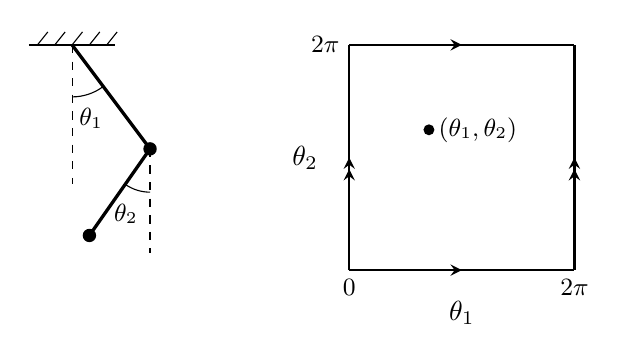
\begin{tikzpicture}[scale=1.1,>=stealth]
        % the pendulum
        \draw[thick] (-0.5,3)--(0.5,3);
        \foreach \x in {-0.4,-0.2,...,0.4} \draw (\x,3)--(\x+0.12,3.15);
        \draw[dashed] (0,3)--(0,1.4);
        \draw[very thick] (0,3)--(0.9,1.8);
        \fill (0.9,1.8) circle (2.2pt);
        \draw[dashed] (0.9,1.8)--(0.9,0.6);
        \draw[very thick] (0.9,1.8)--(0.2,0.8);
        \fill (0.2,0.8) circle (2.2pt);
        \draw (0,2.4) arc[start angle=-90,end angle=-53.1,radius=0.6];
        \node at (0.22,2.15) {\small $\theta_1$};
        \draw (0.9,1.3) arc[start angle=-90,end angle=-124.99,radius=0.5];
        \node at (0.62,1.05) {\small $\theta_2$};
        % the torus as a square
        \begin{scope}[xshift=3.2cm,yshift=0.4cm]
            \draw[thick,->] (0,0)--(1.3,0); \draw[thick] (1.2,0)--(2.6,0);
            \draw[thick,->] (0,2.6)--(1.3,2.6); \draw[thick] (1.2,2.6)--(2.6,2.6);
            \draw[thick,->>] (0,0)--(0,1.3); \draw[thick] (0,1.2)--(0,2.6);
            \draw[thick,->>] (2.6,0)--(2.6,1.3); \draw[thick] (2.6,1.2)--(2.6,2.6);
            \node[below] at (0,0) {\small $0$}; \node[below] at (2.6,0) {\small $2\pi$};
            \node[left] at (0,2.6) {\small $2\pi$};
            \node[below] at (1.3,-0.25) {$\theta_1$}; \node[left] at (-0.25,1.3) {$\theta_2$};
            \fill (0.92,1.62) circle (1.8pt);
            \node[right] at (0.92,1.62) {\small $(\theta_1,\theta_2)$};
        \end{scope}
    \end{tikzpicture}
    \caption{A double pendulum and its configuration space: a square whose opposite sides (marked by single and double arrows) are glued, i.e., the torus $\bbT^2$.}
    \label{fig double pendulum}
\end{figure}

\begin{defn}[Locally Euclidean space]\index{Locally Euclidean space}
    A topological space $X$ is \emph{locally Euclidean of dimension $n$} if every point $x\in X$ has an open neighborhood homeomorphic to an open subset of $\bbR^n$.
\end{defn}
Since an open ball is homeomorphic to $\bbR^n$ (Example~\ref{example homeomorphisms}), we may equally ask for neighborhoods homeomorphic to a ball, or to $\bbR^n$ itself. For this definition to make sense, the number $n$ must be determined by the space.

\begin{prop}[Invariance of dimension]\label{prop invariance of dimension}\index{Invariance of dimension}
    If nonempty open sets $U\subset\bbR^m$ and $V\subset\bbR^n$ are homeomorphic, then $m=n$.
\end{prop}
\begin{proof}[Proof for $\min(m,n)\leq2$]
    We may assume that $m<n$; the case $m=0$ is trivial. Let $h:U\to V$ be a homeomorphism, and first let $m=1$. Pick an open interval $I\subset U$ and a ball $B\subset h(I)$, which exists since $h(I)$ is open in $V$. Then $J=h^{-1}(B)$ is a connected open subset of $I$, i.e., an interval, and $h$ restricts to a homeomorphism $J\setminus\{x\}\cong B\setminus\{h(x)\}$ for any $x\in J$. But the punctured interval is disconnected, while the punctured ball is path-connected for $n\geq2$, as in Example~\ref{example cut points}.

    The case $m=2<n$ is the same argument one dimension up, with connectedness replaced by simple connectedness. Pick $\bf{x}\in U$, a ball $B\ni h(\bf{x})$ in $V$, and a disk $D\ni\bf{x}$ in $h^{-1}(B)$. A small circle around $\bf{x}$ in $D$ generates $\pi_1(D\setminus\{\bf{x}\})\cong\pi_1(\bbS^1)\cong\bbZ$ (Example~\ref{example deformation retracts} and Theorem~\ref{thm pi1 of circle elementary}). Its image is a loop in $B\setminus\{h(\bf{x})\}\simeq\bbS^{n-1}$, which is null-homotopic by Corollary~\ref{cor pi_1(S^n)=0}. Pulling the null-homotopy back by $h^{-1}$, we find that the circle is null-homotopic in $h^{-1}(B)\setminus\{\bf{x}\}$, hence in $\bbR^2\setminus\{\bf{x}\}$. This is a contradiction, since $\bbR^2\setminus\{\bf{x}\}$ deformation retracts onto the circle. The general case requires homology and will be proved in Corollary~\ref{cor invariance of dimension}.
\end{proof}

Being locally Euclidean is far from enough to make a space well-behaved. The line with two origins (Example~\ref{example two origins}, Figure~\ref{fig two origins}) is locally homeomorphic to $\bbR$, but a sequence can converge to two different points in it. At the other extreme, the disjoint union of uncountably many lines $\bigsqcup_{a\in\bbR}\bbR$ is locally Euclidean and Hausdorff, but it is ``too large'': it has uncountably many components, it cannot be embedded in any $\bbR^N$ (whose subspaces are all separable), and we will see that Sard's theorem fails for it. Both pathologies are ruled out by the axioms of \S\ref{Separation Axioms} and \S\ref{sec: topological spaces}.

\begin{defn}[Topological manifold]\index{Manifold!topological}
    A \emph{topological manifold of dimension $n$} is a second countable Hausdorff space that is locally Euclidean of dimension $n$. We write $M^n$ when we want to indicate the dimension.
\end{defn}

\begin{rem*}
    There are also connected examples of Hausdorff locally Euclidean spaces that are not second countable. The most famous one is the \emph{long line}\index{Long line}. To construct it, one glues uncountably many (more precisely, $\omega_1$) half-open intervals $[0,1)$ end to end, removes the initial point, and glues two copies of the resulting \emph{long ray} at their initial ends. It is ``too long'' to be covered by countably many charts.
\end{rem*}

\begin{defn}[Charts]\index{Chart}
    Let $M$ be an $n$-dimensional topological manifold. A \emph{chart} on $M$ is a pair $(U,\varphi)$, where $U\subset M$ is open and $\varphi:U\to\wh U=\varphi(U)$ is a homeomorphism onto an open subset $\wh U\subset\bbR^n$. The values $\bf{x}=\varphi(m)\in\bbR^n$ are the \emph{coordinates}\index{Coordinates} of the point $m\in U$, and the components $x^i=\varphi^i(m)$ of the chart map are the \emph{coordinate functions}. Hence, sometimes we write $(U,\bf{x})$ for the chart. The chart is a \emph{coordinate ball}\index{Coordinate ball} if $\wh U$ is a ball $B_r(\bf{x}_0)$, and a \emph{regular coordinate ball}\index{Coordinate ball!regular} if, in addition, $\varphi$ extends to a chart $\varphi':U'\to B_{r'}(\bf{x}_0)$ with $r'>r$.
\end{defn}
The closure of a regular coordinate ball $U$ is the compact set $\varphi'^{-1}(\wb B_r(\bf{x}_0))$: this set is compact, hence closed in the Hausdorff space $M$, and it is contained in the closure of $U$. Thus regular coordinate balls are \emph{precompact}\index{Precompact set}, i.e., have compact closures.

\begin{example}\label{example topological manifolds}
    \begin{enumerate}
        \item Every open subset of $\bbR^n$, and more generally every open subset of an $n$-manifold, is an $n$-manifold. For instance, the invertible matrices $\GL_n(\bbR)$ form an open subset of $\Mat_n(\bbR)\cong\bbR^{n^2}$ (Example~\ref{example zero sets}), hence an $n^2$-manifold.
        \item \emph{Graphs.} If $U\subset\bbR^n$ is open and $f:U\to\bbR^k$ is continuous, then the graph $\Gamma_f\subset\bbR^{n+k}$ is an $n$-manifold covered by a single chart: the projection $(\bf{x},\bf{y})\mapsto\bf{x}$ (Example~\ref{example homeomorphisms} and Figure~\ref{fig graph chart}).
        \item \emph{Spheres.} The sphere $\bbS^n\subset\bbR^{n+1}$ is Hausdorff and second countable as a subspace of $\bbR^{n+1}$. It is covered by the $2n+2$ open hemispheres $U_i^\pm=\{\pm x^i>0\}$, each of which is the graph of the function $x^i=\pm\sqrt{1-\sum_{j\neq i}(x^j)^2}$ over the open unit ball in the remaining coordinates (Figure~\ref{fig hemisphere charts}). Alternatively, two charts suffice: the stereographic projections from the north and south poles (Examples~\ref{example homeomorphisms} and~\ref{example sphere two charts}).
        \item \emph{Products.}\index{Torus} If $M^m$ and $N^n$ are manifolds, then $M\times N$ is an $(m+n)$-manifold with charts $(U\times V,\varphi\times\psi)$. In particular, the torus $\bbT^n=(\bbS^1)^n$ is an $n$-manifold.
        \item \emph{Projective spaces.}\index{Projective space} Let $U_i\subset\RP^n$ be the set of lines $[\bf{x}]=[x^1:\ldots:x^{n+1}]$ with $x^i\neq0$, and
        \[\varphi_i([\bf{x}])=\Big(\frac{x^1}{x^i},\ldots,\widehat{\frac{x^i}{x^i}},\ldots,\frac{x^{n+1}}{x^i}\Big)\in\bbR^n\]
        (the hat means that the entry is omitted). The set $U_i$ is open, since its preimage in $\bbR^{n+1}\setminus\{0\}$ is. The map $\varphi_i$ is well-defined, continuous by the universal property of the quotient (Proposition~\ref{prop initial final universal}), and bijective with the continuous inverse $\bf{y}\mapsto[y^1:\ldots:y^{i-1}:1:y^i:\ldots:y^n]$. Geometrically, $\varphi_i$ records where a line meets the affine hyperplane $x^i=1$. The space $\RP^n$ is Hausdorff (Example~\ref{example RPn Hausdorff}) and is covered by the $n+1$ charts $U_i$, so it is an $n$-manifold.
    \end{enumerate}
\end{example}

\begin{figure}[tp]
    \centering
    \begin{tikzpicture}[scale=1.2,>=stealth]
        \draw[gray,->] (-0.3,0)--(4.4,0) node[right] {$\bbR^n$};
        \draw[gray,->] (0,-0.3)--(0,2.6) node[above] {$\bbR^k$};
        \draw[very thick] plot[smooth] coordinates {(0.6,1.4) (1.3,2.0) (2.2,1.2) (3.1,1.7) (3.8,1.1)};
        \node[above] at (3.1,1.75) {$\Gamma_f$};
        \draw[thick] (0.6,0)--(3.8,0);
        \node[below] at (0.6,0) {$($}; \node[below] at (3.8,0) {$)$};
        \node[below] at (2.2,-0.25) {$U$};
        \foreach \x/\y in {1.3/2.0,2.2/1.2,3.1/1.7} {
            \fill (\x,\y) circle (1.5pt);
            \draw[dashed,->] (\x,\y-0.08)--(\x,0.08);
            \fill (\x,0) circle (1.5pt);
        }
    \end{tikzpicture}
    \caption{The graph of a continuous function $f:U\to\bbR^k$ is a manifold with a single chart: the vertical projection onto $U$ (dashed arrows).}
    \label{fig graph chart}
\end{figure}

\begin{figure}[tp]
    \centering
    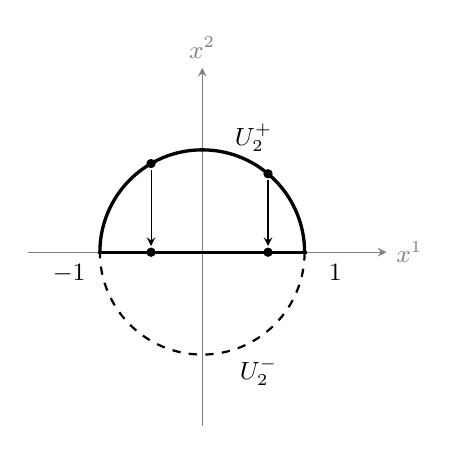
\begin{tikzpicture}[scale=1.3,>=stealth]
        \draw[gray,->] (-1.7,0)--(1.8,0) node[right] {\small $x^1$};
        \draw[gray,->] (0,-1.7)--(0,1.8) node[above] {\small $x^2$};
        \draw[very thick] (1,0) arc[start angle=0,end angle=180,radius=1];
        \draw[thick,dashed] (1,0) arc[start angle=0,end angle=-180,radius=1];
        \draw[very thick] (-0.03,-0.03)++(0,0) (-1.02,0)--(1.02,0);
        \node at (0.5,1.12) {\small $U_2^+$};
        \node at (0.55,-1.17) {\small $U_2^-$};
        \foreach \a in {50,120} {
            \fill ({cos(\a)},{sin(\a)}) circle (1.3pt);
            \draw[->] ({cos(\a)},{sin(\a)-0.06})--({cos(\a)},0.06);
            \fill ({cos(\a)},0) circle (1.3pt);
        }
        \node[below] at (1.3,-0.02) {\small $1$};
        \node[below] at (-1.3,-0.02) {\small $-1$};
    \end{tikzpicture}
    \caption{The upper and lower half-circles $U_2^\pm$ (solid and dashed) are graphs over the open interval $(-1,1)$ (thick), and the vertical projection is a chart on each. The right and left half-circles $U_1^\pm$ are charted by the horizontal projection in the same way.}
    \label{fig hemisphere charts}
\end{figure}

Not every space that looks like a ``nice surface'' is a manifold. The cut point arguments of Example~\ref{example cut points} detect the points where it is not locally Euclidean.

\begin{example}\label{example non-manifolds}
    \begin{enumerate}
        \item The figure eight (Figure~\ref{fig figure eight}) is not a manifold. Every small connected neighborhood of the crossing point falls into four components when the point is removed, while a punctured interval has two components and a punctured ball in $\bbR^n$, $n\geq2$, is connected.
        \item The double cone $C=\{x^2+y^2=z^2\}\subset\bbR^3$ is not a manifold: it is locally homeomorphic to a disk away from the apex, so by invariance of dimension it could only be a $2$-manifold. But removing the apex from a small connected neighborhood of it leaves two components, while a punctured disk is connected (Figure~\ref{fig double cone}). On the other hand, the upper half $C_+=C\cap\{z\geq0\}$ is a manifold, since it is the graph of the continuous function $z=\sqrt{x^2+y^2}$. Its apex is a perfectly good point of a topological manifold, even though the cone is not ``smooth'' there. Detecting such corners requires looking at how $C_+$ sits inside $\bbR^3$ with the help of derivatives, which we will do in \S\ref{sec submanifolds}.
    \end{enumerate}
\end{example}

\begin{figure}[tp]
    \centering
    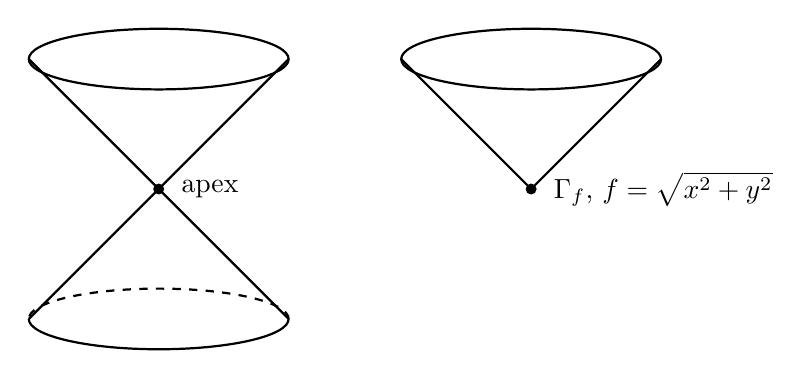
\begin{tikzpicture}[scale=1.1,>=stealth]
        \draw[thick] (0,1.5) ellipse (1.5 and 0.35);
        \draw[thick] (-1.5,1.5)--(1.5,-1.5) (1.5,1.5)--(-1.5,-1.5);
        \draw[thick] (-1.5,-1.5) arc[start angle=180,end angle=360,x radius=1.5,y radius=0.35];
        \draw[thick,dashed] (1.5,-1.5) arc[start angle=0,end angle=180,x radius=1.5,y radius=0.35];
        \fill (0,0) circle (1.8pt);
        \node[right] at (0.15,0) {apex};
        \begin{scope}[xshift=4.3cm]
            \draw[thick] (0,1.5) ellipse (1.5 and 0.35);
            \draw[thick] (-1.5,1.5)--(0,0)--(1.5,1.5);
            \fill (0,0) circle (1.8pt);
            \node[right] at (0.15,0) {$\Gamma_f$, $f=\sqrt{x^2+y^2}$};
        \end{scope}
    \end{tikzpicture}
    \caption{The double cone is not a manifold: removing the apex disconnects every small neighborhood of it. Its upper half is a manifold, being the graph of a continuous function.}
    \label{fig double cone}
\end{figure}

Many spaces of interest, like the closed ball or the closed interval, have a boundary. They are modeled on the closed upper half-space $\wb\bbR^n_+=\{\bf{x}\in\bbR^n\mid x^n\geq0\}$.\index{$\wb\bbR_+^n$}

\begin{defn}[Manifolds with boundary]\index{Manifold!with boundary}
    A \emph{topological $n$-manifold with boundary} is a second countable Hausdorff space $M$ in which every point has a neighborhood homeomorphic to a (relatively) open subset of $\wb\bbR^n_+$. A point is a \emph{boundary point}\index{Boundary of a manifold} if some such homeomorphism maps it to the hyperplane $\partial\wb\bbR^n_+=\{x^n=0\}$, and an \emph{interior point}\index{Interior of a manifold} if it has a neighborhood homeomorphic to an open subset of $\bbR^n$. We write $\partial M$ for the set of boundary points and $\mathring M$ for the set of interior points.
\end{defn}
A point cannot be both: this is the \emph{invariance of the boundary}\index{Invariance of the boundary}, $\partial M\cap\mathring M=\varnothing$. For topological manifolds, this is again a consequence of homology theory \cite[Thm.~1.37]{Lee}. For smooth manifolds, which are all we will need, it follows from the inverse function theorem, see Proposition~\ref{prop smooth invariance of boundary}. A topological manifold in the original sense is thus the same as a manifold with empty boundary. Unless we say otherwise, ``manifold'' means a manifold without boundary.

\begin{example}
    The closed ball $\wb{B^n}$ is a manifold with boundary $\bbS^{n-1}$. The cylinder $\bbS^1\times[0,1]$ is a manifold whose boundary consists of two circles, while the M\"obius band (Figure~\ref{fig square gluings}) has a connected boundary (see the exercise below). More generally, $M\times[0,1]$ is a manifold with boundary $M\times\{0,1\}$ for every manifold $M$.
\end{example}

We now collect the basic topological properties of manifolds. The second countability axiom enters through the following observation: \emph{in a second countable space, every open cover has a countable subcover.} Indeed, for each element $B$ of a countable basis that is contained in some member of the cover, choose one such member; these countably many members cover the space.

\begin{defn}[Paracompactness]\index{Paracompact space}\index{Locally finite collection}
    \begin{enumerate}
        \item A collection of subsets $\{A_\alpha\}$ of a space $X$ is \emph{locally finite} if every $x\in X$ has a neighborhood that meets only finitely many of the sets $A_\alpha$.
        \item A \emph{refinement}\index{Refinement of a cover} of an open cover $\{U_\alpha\}$ is an open cover $\{V_\beta\}$ such that every $V_\beta$ is contained in some $U_\alpha$.
        \item $X$ is \emph{paracompact} if every open cover of $X$ has a locally finite refinement.
    \end{enumerate}
\end{defn}
Local finiteness is stronger than asking that every point lies in only finitely many $A_\alpha$: every point of $\bbR$ lies in only finitely many of the intervals $(0,\frac1k)$, $k\in\bbN$, but every neighborhood of $0$ meets all of them.

\begin{thm}[{{\cite[Thms.~1.15, 1.16]{Lee}}}]\label{thm properties of manifolds}
    Let $M$ be a topological $n$-manifold. Then
    \begin{enumerate}[label=(\alph*)]
        \item $M$ has a countable basis consisting of regular coordinate balls;
        \item $M$ is locally compact and locally path-connected; its components are open and coincide with its path components, and there are at most countably many of them;
        \item every open cover of $M$ has a countable, locally finite refinement consisting of regular coordinate balls. In particular, $M$ is paracompact;
        \item the fundamental group of $M$ is countable.
    \end{enumerate}
\end{thm}
\begin{proof}
    (a) Let $(U,\varphi)$ be a chart. The balls $B_r(\bf{q})$ with rational center and rational radius, such that $\wb B_{r'}(\bf{q})\subset\wh U$ for some $r'>r$, form a countable basis of $\wh U$, so their preimages are a countable basis of $U$ consisting of regular coordinate balls. Countably many charts cover $M$ by second countability, and the union of their bases is the required basis of $M$.

    (b) Regular coordinate balls are precompact and path-connected, so $M$ is locally compact and locally path-connected. By Lemma~\ref{lem locally path connected}, its components are open and coincide with path components. Each component contains a basis element from (a), and these are different for different components, so there are countably many components.

    (c) By (b) and Proposition~\ref{prop compact exhaustion}, there is an exhaustion of $M$ by compact sets $K_1\subset K_2\subset\ldots$ with $K_i\subset\Int K_{i+1}$; put $K_0=K_{-1}=\varnothing$. Given an open cover $\mathcal{U}$, the compact ``shell'' $K_{i+1}\setminus\Int K_i$ lies in the open ``shell'' $\Int K_{i+2}\setminus K_{i-1}$ (Figure~\ref{fig exhaustion shells}). By (a), every point of the compact shell has a regular coordinate ball around it that lies both in the open shell and in some member of $\mathcal{U}$, and finitely many of these balls cover the compact shell. All these balls together, $i=0,1,2,\ldots$, form a countable refinement of $\mathcal U$ that covers $M$. It is locally finite: a point lies in some open set $\Int K_{j}$, and the balls chosen at stage $i$ avoid $K_{i-1}$, so only those from the finitely many stages $i\leq j$ can meet $\Int K_j$.

    (d) See the cited reference.
\end{proof}

\begin{figure}[tp]
    \centering
    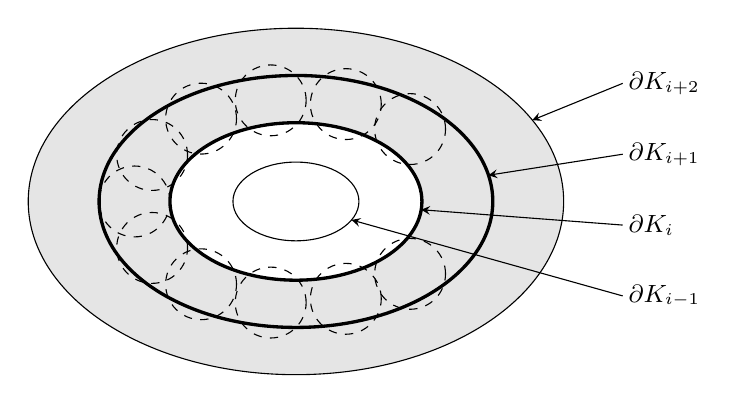
\begin{tikzpicture}[scale=1.0,>=stealth]
        \fill[gray!20,even odd rule] (0,0) ellipse (3.4 and 2.2) (0,0) ellipse (1.6 and 1.0);
        \draw (0,0) ellipse (0.8 and 0.5);
        \draw[very thick] (0,0) ellipse (1.6 and 1.0);
        \draw[very thick] (0,0) ellipse (2.5 and 1.6);
        \draw (0,0) ellipse (3.4 and 2.2);
        \foreach \a in {45,72,...,320} \draw[dashed] ({2.05*cos(\a)},{1.3*sin(\a)}) circle (0.45);
        \node[right] at (4.1,1.50) {\small $\partial K_{i+2}$};
        \draw[->] (4.15,1.50)--(3.002,1.033);
        \node[right] at (4.1,0.60) {\small $\partial K_{i+1}$};
        \draw[->] (4.15,0.60)--(2.445,0.333);
        \node[right] at (4.1,-0.30) {\small $\partial K_i$};
        \draw[->] (4.15,-0.30)--(1.591,-0.105);
        \node[right] at (4.1,-1.20) {\small $\partial K_{i-1}$};
        \draw[->] (4.15,-1.20)--(0.706,-0.235);
    \end{tikzpicture}
    \caption{Each $K_j$ is the whole region inside the curve $\partial K_j$. The compact shell $K_{i+1}\setminus\Int K_i$ between the two thick curves is covered by finitely many small balls (dashed; only some are shown), all contained in the larger open shell $\Int K_{i+2}\setminus K_{i-1}$ (shaded).}
    \label{fig exhaustion shells}
\end{figure}

In particular, by (b), a manifold is connected iff it is path-connected.

Paracompactness is often used in place of second countability in the definition of manifolds. The two definitions differ only in how many components are allowed.

\begin{prop}\label{prop paracompact vs second countable}\index{Paracompact space}\index{Metrizable space}
    For a Hausdorff, locally Euclidean space $X$, the following are equivalent:
    \begin{enumerate}
        \item every component of $X$ is second countable;
        \item $X$ is paracompact;
        \item $X$ is metrizable.
    \end{enumerate}
    Moreover, $X$ is second countable iff these conditions hold and $X$ has at most countably many components. In particular, for connected $X$, second countability, paracompactness and metrizability are equivalent.
\end{prop}
\begin{proof}
    The components of $X$ are open, since $X$ is locally connected, so $X$ is their disjoint union. A countable union of second countable open sets is second countable, and conversely, a second countable space has countably many components, as in Theorem~\ref{thm properties of manifolds}(b). This proves the last statement.

    (1)$\Rightarrow$(2): By Theorem~\ref{thm properties of manifolds}(c), each component is paracompact, and a disjoint union of paracompact spaces is paracompact.

    (2)$\Rightarrow$(1): Let $C$ be a component. It is closed in $X$, hence paracompact. Refine the cover of $C$ by precompact coordinate balls to a locally finite cover $\{V_\beta\}$ by (necessarily precompact) open sets. A compact set meets only finitely many $V_\beta$. So, starting from $K_1=\wb{V_{\beta_0}}$ and letting $K_{j+1}$ be the union of the closures of the $V_\beta$ that meet $K_j$, we get an increasing sequence of compact sets. Their union is open and closed in $C$: a point of $K_j$, or of the closure of $\bigcup_jK_j$, lies in some $V_\beta$ that meets some $K_j$, and then $V_\beta\subset K_{j+1}$. By connectedness, $C=\bigcup_jK_j$. Each $K_j$ is covered by finitely many coordinate balls, so $C$ is covered by countably many second countable open sets, and is second countable.

    (1)$\Rightarrow$(3): Each component is second countable and regular: if $x\notin A$ with $A$ closed, a closed coordinate ball $\wb B$ around $x$ that misses $A$ is compact, hence closed, and $B$ and $X\setminus\wb B$ separate $x$ from $A$. So each component is metrizable by the Urysohn metrization theorem, which we do not prove. Replacing the metric $\rho$ on each component by $\min(\rho,1)$ (Example~\ref{example bounded metric}) and declaring points in different components to be at distance $1$ gives a metric on $X$.

    (3)$\Rightarrow$(2) is Stone's theorem: every metric space is paracompact. We do not prove it.
\end{proof}

Thus the uncountable union of lines above is paracompact and metrizable, but not second countable, while the long line is connected, but has none of these three properties. We will see in \S\ref{sec partitions of unity} that, for smooth manifolds, a fourth equivalent condition is the existence of smooth partitions of unity.

\begin{xca}
    \begin{enumerate}
        \item Show that $\bbR^n\setminus\{0\}\cong\bbS^{n-1}\times\bbR$.
        \item Show that the boundary of the M\"obius band is homeomorphic to a circle.
        \item Show that every element of $\SO_3$ is a rotation by an angle $\theta\in[0,\pi]$ around an axis, and deduce that $\SO_3$ is homeomorphic to the closed ball of radius $\pi$ with antipodal points of its boundary identified, which is $\RP^3$. In particular, the configuration space of a rigid body with a fixed point is a $3$-manifold. (See also Example~\ref{example su2 and so3}.)
    \end{enumerate}
\end{xca}

\begin{rem}[Classification of $1$-manifolds]\label{rem classification of 1-manifolds}\index{Classification of $1$-manifolds}
    Every connected $1$-manifold is homeomorphic to $\bbR$ or $\bbS^1$, and every connected $1$-manifold with nonempty boundary is homeomorphic to $[0,1)$ or $[0,1]$. A short proof for smooth $1$-manifolds can be found in the appendix of \cite{MilnorTDV}. In particular, a compact $1$-manifold with boundary is a finite disjoint union of circles and closed intervals, so its boundary consists of an \emph{even} number of points.
\end{rem}


\section{Smooth structures}

What does it mean for a function $f:\bbS^2\to\bbR$ to be differentiable? The natural answer is to require that $f\circ\varphi^{-1}$ be differentiable for every chart $(U,\varphi)$. But on a topological manifold, this condition depends on the chart. If $(U,\varphi)$ and $(V,\psi)$ are two charts, then on the overlap $f\circ\psi^{-1}=(f\circ\varphi^{-1})\circ(\varphi\circ\psi^{-1})$, and the \emph{transition map} $\varphi\circ\psi^{-1}$ is only a homeomorphism. For example, both $x\mapsto x$ and $x\mapsto x^3$ are charts on $\bbR$, and the function $f(x)=x$ is differentiable in the first chart but not in the second, where it becomes $y\mapsto y^{1/3}$. To do calculus, we must therefore select a class of charts whose transition maps are smooth.

\begin{defn}[Atlas]\index{Atlas!Topological}
    An \emph{atlas} on a topological manifold $M$ is a collection of charts $\mathcal{A}=\{(U_\alpha,\varphi_\alpha)\}$ such that $\bigcup_\alpha U_\alpha=M$.
\end{defn}
Throughout the book, for an atlas as above we write $U_{\alpha\beta}=U_\alpha\cap U_\beta$, $U_{\alpha\beta\gamma}=U_\alpha\cap U_\beta\cap U_\gamma$, and so on.

\begin{defn}[Smooth atlas]\index{Atlas!Smooth}\index{Transition maps}
    The \emph{transition maps} of an atlas are the homeomorphisms
    \[\varphi_{\beta\alpha}=\varphi_\beta\circ\varphi_\alpha^{-1}:\varphi_\alpha(U_{\alpha\beta})\to\varphi_\beta(U_{\alpha\beta})\]
    between open subsets of $\bbR^n$ (Figure~\ref{fig atlas}). The atlas is \emph{smooth} (or of class $C^k$, or \emph{analytic}, i.e., of class $C^\omega$) if all of its transition maps are smooth (respectively, of class $C^k$, or real analytic) in the sense of multivariable calculus. Two charts are \emph{compatible}\index{Atlas!compatible} if the transition maps between them are smooth, and two smooth atlases are \emph{compatible} if their union is still a smooth atlas.
\end{defn}

\begin{figure}[tp]
    \centering
    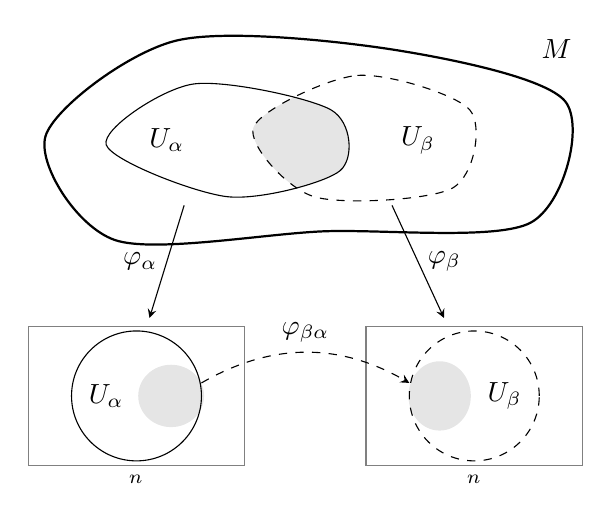
\begin{tikzpicture}[scale=1.1,>=stealth]
        % the manifold
        \begin{scope}
            \clip plot[smooth cycle] coordinates {(-2.3,3.1) (-1.3,3.8) (0.3,3.5) (0.4,2.8) (-0.9,2.5)};
            \fill[gray!20] plot[smooth cycle] coordinates {(-0.6,3.3) (0.6,3.9) (1.9,3.5) (1.7,2.6) (0.1,2.5)};
        \end{scope}
        \draw[thick] plot[smooth cycle] coordinates {(-3,3.2) (-1.5,4.3) (1,4.2) (3,3.6) (2.6,2.2) (0.2,2.1) (-2.2,2.0)};
        \node at (2.9,4.2) {$M$};
        \draw plot[smooth cycle] coordinates {(-2.3,3.1) (-1.3,3.8) (0.3,3.5) (0.4,2.8) (-0.9,2.5)};
        \draw[dashed] plot[smooth cycle] coordinates {(-0.6,3.3) (0.6,3.9) (1.9,3.5) (1.7,2.6) (0.1,2.5)};
        \node at (-1.6,3.15) {$U_\alpha$};
        \node at (1.3,3.15) {$U_\beta$};
        % the images
        \draw[gray] (-3.2,-0.6) rectangle (-0.7,1.0);
        \draw[gray] (0.7,-0.6) rectangle (3.2,1.0);
        \fill[gray!20] (-1.55,0.2) ellipse (0.38 and 0.36);
        \fill[gray!20] (1.55,0.2) ellipse (0.36 and 0.4);
        \draw (-1.95,0.2) circle (0.75);
        \draw[dashed] (1.95,0.2) circle (0.75);
        \node at (-2.3,0.2) {$\wh U_\alpha$};
        \node at (2.3,0.2) {$\wh U_\beta$};
        \node[below] at (-1.95,-0.6) {$\bbR^n$};
        \node[below] at (1.95,-0.6) {$\bbR^n$};
        \draw[->] (-1.4,2.4)--(-1.8,1.1) node[midway,left] {$\varphi_\alpha$};
        \draw[->] (1.0,2.4)--(1.6,1.1) node[midway,right] {$\varphi_\beta$};
        \draw[->,dashed] (-1.2,0.35) to[bend left=30] node[midway,above] {$\varphi_{\beta\alpha}$} (1.2,0.35);
    \end{tikzpicture}
    \caption{Two overlapping charts. The transition map $\varphi_{\beta\alpha}=\varphi_\beta\circ\varphi_\alpha^{-1}$ (dashed arrow) is a map between the images of the overlap $U_{\alpha\beta}$ (shaded) in two copies of $\bbR^n$.}
    \label{fig atlas}
\end{figure}

Compatibility of smooth atlases is an equivalence relation. Only transitivity needs a comment. If $\mathcal{A}_1$ and $\mathcal{A}_2$ are compatible, and $\mathcal{A}_2$ and $\mathcal{A}_3$ are compatible, then near each point $\varphi_\alpha(m)$ the transition map from a chart $\varphi_\alpha\in\mathcal{A}_1$ to a chart $\varphi_\gamma\in\mathcal{A}_3$ factors as $\varphi_\gamma\circ\varphi_\alpha^{-1}=(\varphi_\gamma\circ\varphi_\beta^{-1})\circ(\varphi_\beta\circ\varphi_\alpha^{-1})$ through any chart $\varphi_\beta\in\mathcal{A}_2$ around $m$. So it is smooth, because smoothness is a local property. Each equivalence class contains a unique \emph{maximal}\index{Atlas!maximal} atlas, namely the union of all atlases in the class.

\begin{defn}[Smooth structure]\index{Differentiable structure}\index{Smooth structure}\index{Manifold!smooth}
    A \emph{smooth structure} (or a $C^k$, or an analytic structure) on a topological manifold $M$ is an equivalence class $[\mathcal{A}]$ of smooth (respectively, $C^k$, or $C^\omega$) atlases on it, or equivalently, a maximal smooth atlas. A \emph{smooth manifold} is a pair $(M,[\mathcal{A}])$ consisting of a topological manifold and a smooth structure on it. The charts of the maximal atlas are called \emph{smooth charts}\index{Chart!smooth}.
\end{defn}

\begin{example}\label{example smooth atlases}
    \begin{enumerate}
        \item \emph{The circle.} The angle $\theta$ gives two charts on $\bbS^1\subset\bbC$: $\theta_1:\bbS^1\setminus\{1\}\to(0,2\pi)$ and $\theta_2:\bbS^1\setminus\{-1\}\to(-\pi,\pi)$, both inverse to $\theta\mapsto\rme^{\rmi\theta}$. The overlap consists of the upper and lower open half-circles, and the transition map $\theta_2\circ\theta_1^{-1}$ is the identity on $(0,\pi)$ and $\theta\mapsto\theta-2\pi$ on $(\pi,2\pi)$. Both are smooth, so this is a smooth (even analytic) atlas.
        \item \emph{Spheres.} The two stereographic charts $\varphi_N,\varphi_S$ of $\bbS^n$ have the transition map $\varphi_S\circ\varphi_N^{-1}(\bf{y})=\bf{y}/\lvert\bf{y}\rvert^2$ on $\bbR^n\setminus\{0\}$ (Example~\ref{example sphere two charts}), the inversion in the unit sphere. It is smooth and is its own inverse, so these charts form a smooth atlas. The hemisphere charts of Example~\ref{example topological manifolds} form another smooth atlas, compatible with the first one (Exercise~\ref{xca hemisphere stereographic}).
        \item \emph{Projective spaces.} For the charts $\varphi_i$ on $\RP^n$ of Example~\ref{example topological manifolds}, the transition map $\varphi_j\circ\varphi_i^{-1}$ inserts $1$ as the $i$-th entry of $\bf{y}\in\bbR^n$, divides by the $j$-th entry (which is nonzero on the overlap) and deletes it. Its components are rational functions with nonvanishing denominators, hence smooth.
        \item \emph{Vector spaces.} A finite-dimensional real vector space $V$ has a canonical smooth structure: every linear isomorphism $V\to\bbR^n$ is a global chart, and any two of them differ by an invertible linear map, which is smooth. In particular, $\Mat_n(\bbR)\cong\bbR^{n^2}$ and its open subset $\GL_n(\bbR)$ are smooth manifolds. Complex vector spaces are smooth manifolds as real vector spaces.
        \item \emph{Open subsets and products.} An open subset of a smooth manifold inherits a smooth structure by restricting the charts, and a product of smooth manifolds has the smooth atlas of products of charts. For example, the torus $\bbT^n$ is a smooth manifold.
        \item \emph{A different structure on the line.} The single chart $\psi(x)=x^3$ is a smooth atlas on $\bbR$. It is not compatible with the standard chart $\varphi(x)=x$, since $\varphi\circ\psi^{-1}(y)=y^{1/3}$ is not smooth. So the line has at least two different smooth structures (and, using $x\mapsto x^{2k+1}$, infinitely many). We will see shortly that they are nevertheless ``the same'' in a different sense.
        \item \emph{The cone.} The upper half $C_+$ of the double cone (Example~\ref{example non-manifolds}) has the single chart $(x,y,z)\mapsto(x,y)$, so it is a smooth manifold. Its corner at the apex is invisible to the smooth structure: it is a property of how $C_+$ sits inside $\bbR^3$, which we will capture by the notion of an embedded submanifold in \S\ref{sec submanifolds}.
    \end{enumerate}
\end{example}

\begin{xca}\label{xca hemisphere stereographic}
    Compute the transition map between the stereographic chart $\varphi_N$ and the hemisphere chart on $U_{n+1}^-=\{x^{n+1}<0\}$ of $\bbS^n$, and show that the hemisphere and stereographic atlases are compatible.
\end{xca}

From now on, ``manifold'' means ``smooth manifold'', unless we say otherwise. The smooth structure allows us to define smooth maps chart by chart.

\begin{defn}[Smooth maps]\index{Smooth map}
    Let $M$ and $N$ be smooth manifolds. A continuous map $f:M\to N$ is \emph{smooth} if for every pair of smooth charts $(U,\varphi)$ on $M$ and $(V,\psi)$ on $N$, the \emph{local representative}\index{Local representative}
    \[\wh f=\psi\circ f\circ\varphi^{-1}:\varphi\big(U\cap f^{-1}(V)\big)\to\psi(V)\]
    is smooth. The set of smooth maps is denoted by $C^\infty(M,N)$, and $C^\infty(M)=C^\infty(M,\bbR)$ is the algebra of \emph{smooth functions}\index{Smooth function} on $M$. Smooth manifolds and smooth maps form the category $\mathsf{Man}^\infty$.
\end{defn}
Continuity is assumed so that the domains $U\cap f^{-1}(V)$ are open. Since local representatives in different charts differ by composition with transition maps, it suffices to check smoothness for the charts of any two atlases. For the same reason, composites of smooth maps are smooth.

\begin{xca}\label{xca charts are smooth}
    Show that every smooth chart $\varphi:U\to\bbR^n$ is a smooth map, where $\bbR^n$ carries its standard structure.
\end{xca}

\begin{example}\label{example smooth maps}
    \begin{enumerate}
        \item The inclusion $\bbS^n\hookrightarrow\bbR^{n+1}$ is smooth. In the hemisphere chart on $U_{n+1}^+$, its local representative is $\bf{y}\mapsto(\bf{y},\sqrt{1-\lvert\bf{y}\rvert^2})$, which is smooth on the open unit ball, and similarly for the other hemispheres.
        \item The projection $\bbR^{n+1}\setminus\{0\}\to\RP^n$, $\bf{x}\mapsto[\bf{x}]$, and its restriction $\bbS^n\to\RP^n$ are smooth: in the chart $\varphi_i$ the first one is $\bf{x}\mapsto(x^1/x^i,\ldots,x^{n+1}/x^i)$ with the $i$-th entry omitted.
        \item On $\GL_n(\bbR)$, matrix multiplication and inversion are smooth: the entries of $AB$ are polynomials in the entries of $A$ and $B$, and by Cramer's rule the entries of $A^{-1}$ are polynomials divided by $\det A\neq0$. The determinant $\det:\Mat_n(\bbR)\to\bbR$ is a polynomial, hence smooth.
    \end{enumerate}
\end{example}

\begin{rem}
    By Exercise~\ref{xca charts are smooth}, the smooth structure determines which functions on open subsets of $M$ are smooth. Conversely, these functions determine the smooth structure: a chart $(U,\varphi)$ is smooth iff a function $g$ on an open subset of $\varphi(U)$ is smooth exactly when $g\circ\varphi$ is. This suggests an alternative definition of manifolds, popular in algebraic geometry, in which one specifies the algebras of smooth functions on all open subsets of $M$ instead of an atlas.
\end{rem}

\begin{defn}[Diffeomorphisms]\index{Diffeomorphism}
    A smooth map $f:M\to N$ is a \emph{diffeomorphism} if it is bijective and its inverse is smooth. Diffeomorphisms are the isomorphisms in $\mathsf{Man}^\infty$. They are, in particular, homeomorphisms.
\end{defn}

\begin{example}
    \begin{enumerate}
        \item Different smooth structures can be diffeomorphic. The map $\psi(x)=x^3$ is a diffeomorphism from $\bbR$ with the structure given by the chart $\psi$ to $\bbR$ with the standard structure: its local representative in these two charts is $\varphi\circ\psi\circ\psi^{-1}=\id$. In fact, $\bbR$ has only one smooth structure up to diffeomorphism, and so does $\bbS^1$ (Exercise~\ref{xca circle structures}).
        \item The space $\bbR^n$ has a unique smooth structure up to diffeomorphism for all $n\neq4$. In contrast, $\bbR^4$ admits \emph{uncountably many} pairwise non-diffeomorphic smooth structures. This is one of the reasons why four-dimensional topology is especially intricate, and many of its fundamental problems are still open \cite{smooth.structures}.
        \item The first manifolds found to carry several non-diffeomorphic smooth structures were spheres. Milnor's \emph{exotic spheres}\index{Exotic sphere} are homeomorphic but not diffeomorphic to $\bbS^7$; there are $28$ smooth structures on $\bbS^7$ up to orientation-preserving diffeomorphism.
        \item All topological manifolds of dimension at most $3$ have smooth structures, unique up to diffeomorphism. In every dimension $n\geq4$, there are compact topological manifolds that admit no smooth structure at all.
    \end{enumerate}
\end{example}

\begin{xca}\label{xca circle structures}
    Show that every smooth structure on $\bbS^1$ is diffeomorphic to the standard one. \emph{Hint:} parametrize the circle by a smooth ``arclength'' coordinate.
\end{xca}

\begin{rem}
    A manifold may carry several nested kinds of structure. A $C^1$ manifold has a maximal $C^1$ atlas, which may contain $C^\infty$ sub-atlases, and these in turn may contain analytic sub-atlases. Whitney proved that every maximal $C^1$ atlas contains a $C^\infty$ atlas, and even an analytic one, and that the resulting smooth structure is unique up to diffeomorphism (see Theorem~\ref{thm whitney embedding} and the remark after it). This is why one mostly works either with topological manifolds or directly with smooth ones. Between these two levels, on the other hand, the examples above show that existence and uniqueness both fail. We will meet this idea many times throughout this book: Lie groups (\Chap~\ref{ch Lie I}), fiber bundles, and Cartan geometries can all be defined by special atlases compatible with the smooth structure.
\end{rem}

Smooth manifolds with boundary are modeled on the half-space $\wb\bbR^n_+$. To make sense of smooth maps between its open subsets, we use the following convention: a map $f:A\to\bbR^k$ defined on an \emph{arbitrary} subset $A\subset\bbR^n$ is \emph{smooth} if every point of $A$ has an open neighborhood $W\subset\bbR^n$ and a smooth map $\wt f:W\to\bbR^k$ that agrees with $f$ on $A\cap W$.

\begin{defn}[Smooth manifolds with boundary]\index{Manifold!with boundary}
    A \emph{smooth manifold with boundary} is a topological manifold with boundary $M$ together with a maximal atlas of charts $\varphi_\alpha:U_\alpha\to\wh U_\alpha$ onto relatively open subsets $\wh U_\alpha\subset\wb\bbR^n_+$ whose transition maps are smooth in the above sense. Smooth maps, diffeomorphisms, and so on, are defined exactly as before.
\end{defn}

\begin{example}
    \begin{enumerate}
        \item The closed ball $\wb{B^n}$ is a smooth manifold with boundary. Near the boundary sphere, a chart is given by $\bf{x}\mapsto\big(\varphi(\bf{x}/\lvert\bf{x}\rvert),\,1-\lvert\bf{x}\rvert\big)$, where $\varphi$ is a chart of $\bbS^{n-1}$, and the interior is charted by the identity.
        \item The function $x\mapsto\sqrt x$ is not smooth on $[0,\infty)$ with its standard structure, since it does not extend to a smooth function near $0$. But it is a homeomorphism $[0,\infty)\to[0,\infty)$, so it can be taken as a chart defining a new smooth structure on $[0,\infty)$. In this structure, $\sqrt x$ is smooth, because its local representative is the identity.
    \end{enumerate}
\end{example}

\begin{rem}
    Similarly, one can define \emph{manifolds with corners}\index{Manifold!with corners} using charts with values in quadrants, octants, and so on. For example, the closed cube $[0,1]^n$ is a manifold with corners. As topological manifolds with boundary, the cube and the ball are homeomorphic (Example~\ref{example homeomorphisms}). The corners of the cube are not visible to the topology, just like the apex of the cone.
\end{rem}

Smooth structures describe the most basic level of what one may call ``geometry''. Each kind of structure comes with its own natural constructions: the tangent spaces of \S\ref{sec tangent spaces} are a first example.

\begin{intu*}
    Keeping in mind that one may be interested in a particular narrowly defined category of structures (smooth, analytic, Lie groups, fiber bundles, and so on), we can broadly define differential geometry as the study of natural constructions (functors) on categories of differentiable structures. These functors can take values in various categories: sets, groups, vector spaces, algebras, manifolds, and so on. Oftentimes, however, we are interested in certain non-natural structures as well, which require a manual choice of some \emph{geometric structure} that cannot be described simply by a kind of atlas. For example, a Riemannian metric is a choice of a positive definite inner product on each tangent space, which is not a functorial construction. The study of such structures is also part of differential geometry, which leads to the following slogan:
    \begin{gather*}
        \boxed{\begin{array}{c}
        \text{The basic task of differential geometry is to study}\\
        \text{natural constructions (functors) on categories}\\
        \text{of differentiable and geometric structures.}
        \end{array}}
    \end{gather*}
    This definition is too broad, since it covers many purely topological or algebraic properties of manifolds. We will be able to give a precise definition of geometric structures at the end of \Part~\ref{part Lie group actions}, and appropriately refine this definition after that, see the opening of \Part~\ref{Part Structured Geom I} and of \Chap~\ref{ch equivalence problems}.
\end{intu*}


\section{Inverse and implicit function theorems}\label{sec inverse function theorem}

All local results about smooth manifolds ultimately rest on two theorems of multivariable calculus, which we now prove. The idea behind both is that a smooth map behaves near a point like its linearization. A linear map $\bbR^n\to\bbR^n$ is invertible iff its matrix is, and a linear system $A\bf{x}+B\bf{y}=\bf{c}$ can be solved for $\bf{y}$ iff $B$ is invertible. The nonlinear versions hold locally, under the same conditions on the derivative.

For a smooth map $f:U\to\bbR^k$ on an open set $U\subset\bbR^n$, we write $Df(\bf{x})$ for its derivative at $\bf{x}$, i.e., the linear map given by the Jacobi matrix $\big(\partial f^i/\partial x^j(\bf{x})\big)$, and we measure linear maps by the operator norm $\lVert\cdot\rVert$ (Example~\ref{example matrix norms}). If the segment between $\bf{x}$ and $\bf{x}'$ lies in $U$, then integrating the derivative along it gives
\[\begin{gathered}
    f(\bf{x}')-f(\bf{x})=\int_0^1Df\big(\bf{x}+t(\bf{x}'-\bf{x})\big)(\bf{x}'-\bf{x})\dd t,\\
    \text{so}\quad\lvert f(\bf{x}')-f(\bf{x})\rvert\leq\sup_{t\in[0,1]}\big\lVert Df\big(\bf{x}+t(\bf{x}'-\bf{x})\big)\big\rVert\,\lvert\bf{x}'-\bf{x}\rvert.
\end{gathered}\]
This \emph{mean value inequality}\index{Mean value inequality} is all the analysis we need.

\begin{thm}[\gls{inmt}]\label{InMT}\index{Theorem!Inverse mapping}
    Let $U\subset\bbR^n$ be open, $f\in C^\infty(U,\bbR^n)$, and $\bf{a}\in U$. If $Df(\bf{a})$ is invertible, then there are open neighborhoods $U_{\bf{a}}\subset U$ of $\bf{a}$ and $V$ of $f(\bf{a})$ such that $\restr{f}{U_{\bf{a}}}:U_{\bf{a}}\to V$ is a diffeomorphism.
\end{thm}
\begin{proof}
    Replacing $f$ by $\bf{x}\mapsto Df(\bf{a})^{-1}\big(f(\bf{a}+\bf{x})-f(\bf{a})\big)$, we may assume that $\bf{a}=0$, $f(0)=0$, and $Df(0)=\rmI_n$. Then $f$ is a small perturbation of the identity: the map $g(\bf{x})=\bf{x}-f(\bf{x})$ has $Dg(0)=0$. By continuity of $Dg$, we can choose $r>0$ such that $\lVert Dg\rVert\leq\frac12$ on the closed ball $\wb B_r(0)\subset U$. By the mean value inequality, $g$ is a contraction there:
    \[\lvert g(\bf{x})-g(\bf{x}')\rvert\leq\tfrac12\lvert\bf{x}-\bf{x}'\rvert.\]

    \emph{Existence and uniqueness of the inverse.} The equation $f(\bf{x})=\bf{y}$ is equivalent to the fixed point equation $\bf{x}=T_{\bf{y}}(\bf{x})$ for $T_{\bf{y}}(\bf{x})=\bf{y}+g(\bf{x})$. For $\lvert\bf{y}\rvert<\frac r2$, the map $T_{\bf{y}}$ sends $\wb B_r(0)$ into itself, since $\lvert T_{\bf{y}}(\bf{x})\rvert\leq\lvert\bf{y}\rvert+\frac12\lvert\bf{x}\rvert<r$, and it is a contraction. By the contraction mapping principle (Theorem~\ref{thm contraction}), applied to the complete metric space $\wb B_r(0)$, the equation $f(\bf{x})=\bf{y}$ has a unique solution $\bf{x}\in\wb B_r(0)$, which actually lies in the open ball $B_r(0)$. Thus, $f$ maps $U_0=B_r(0)\cap f^{-1}(V)$ bijectively onto $V=B_{r/2}(0)$.

    \emph{The inverse is Lipschitz.} Since $\bf{x}=f(\bf{x})+g(\bf{x})$,
    \[\lvert\bf{x}-\bf{x}'\rvert\leq\lvert f(\bf{x})-f(\bf{x}')\rvert+\tfrac12\lvert\bf{x}-\bf{x}'\rvert,\quad\text{so}\quad\lvert\bf{x}-\bf{x}'\rvert\leq2\lvert f(\bf{x})-f(\bf{x}')\rvert.\]

    \emph{The inverse is smooth.} For $\bf{x}\in B_r(0)$, the matrix $Df(\bf{x})=\rmI_n-Dg(\bf{x})$ is invertible by the Neumann series (Example~\ref{example Neumann series}). Let $\bf{y}=f(\bf{x})$ and $\bf{y}+\bf{k}=f(\bf{x}+\bf{h})$. Then $\bf{k}=Df(\bf{x})\bf{h}+o(\lvert\bf{h}\rvert)$, and since $\lvert\bf{h}\rvert\leq2\lvert\bf{k}\rvert$, we get $\bf{h}=Df(\bf{x})^{-1}\bf{k}+o(\lvert\bf{k}\rvert)$. So $f^{-1}$ is differentiable, with
    \[D(f^{-1})(\bf{y})=Df\big(f^{-1}(\bf{y})\big)^{-1}.\]
    The right-hand side is the composite of $f^{-1}$, $Df$, and matrix inversion, which is smooth on $\GL_n(\bbR)$ (Example~\ref{example smooth maps}). If $f^{-1}$ is of class $C^k$, then so is the right-hand side, and $f^{-1}$ is of class $C^{k+1}$. By induction, $f^{-1}$ is smooth.
\end{proof}

Thus, a smooth map with an everywhere invertible derivative is a \emph{local diffeomorphism}\index{Local diffeomorphism}: every point has a neighborhood that it maps diffeomorphically onto an open set (see also Definition~\ref{def immersion submersion}). The proof works verbatim for maps of class $C^k$, $k\geq1$, and also for maps between Banach spaces (\S\ref{sec: completeness}), where it is the basis of infinite-dimensional analysis. Both the invertibility of the derivative and its continuity are essential, and the conclusion is only local.

\begin{example}\label{example InMT hypotheses}
    \begin{enumerate}
        \item The map $x\mapsto x^3$ is a smooth homeomorphism of $\bbR$, but its inverse $y\mapsto y^{1/3}$ is not differentiable at $0$, where the derivative of $x^3$ vanishes.
        \item The function $f(x)=x+2x^2\sin\frac1x$, $f(0)=0$, is differentiable with $f'(0)=1$, but it is not injective on any neighborhood of $0$. Indeed, $f'(x)=1+4x\sin\frac1x-2\cos\frac1x$ takes the value $-1$ at all points $x=\frac1{2\pi k}$. The derivative is not continuous at $0$, and the theorem needs continuous derivatives.
        \item The theorem is purely local. The polar coordinate map $P(r,\theta)=(r\cos\theta,r\sin\theta)$ on $(0,\infty)\times\bbR$ has $\det DP=r>0$, so it is a local diffeomorphism, but it is far from injective (Figure~\ref{fig polar coordinates}). The complex exponential $z\mapsto\rme^z$ is the same map in disguise.
    \end{enumerate}
\end{example}

\begin{figure}[tp]
    \centering
    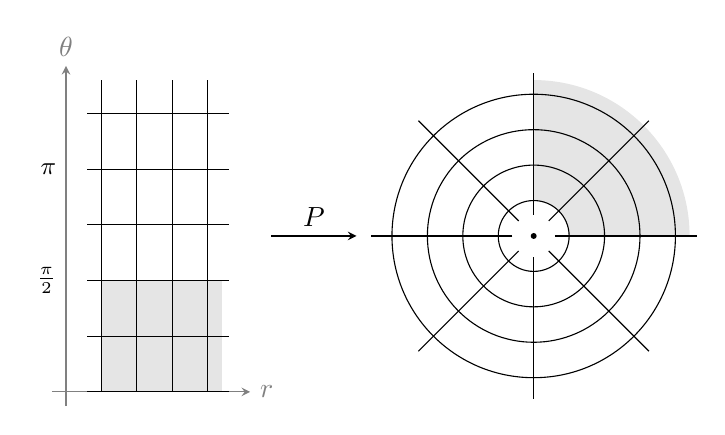
\begin{tikzpicture}[scale=0.9,>=stealth]
        \draw[gray,->] (-0.2,0)--(2.6,0) node[right] {$r$};
        \draw[gray,->] (0,-0.2)--(0,4.6) node[above] {$\theta$};
        \fill[gray!20] (0.5,0)--(2.2,0)--(2.2,1.57)--(0.5,1.57)--cycle;
        \foreach \r in {0.5,1.0,1.5,2.0} \draw (\r,0)--(\r,4.4);
        \foreach \t in {0,0.785,1.571,2.356,3.142,3.927} \draw (0.3,\t)--(2.3,\t);
        \node[left] at (0,1.571) {\small $\frac\pi2$};
        \node[left] at (0,3.142) {\small $\pi$};
        \draw[->] (2.9,2.2)--(4.1,2.2) node[midway,above] {$P$};
        \begin{scope}[xshift=6.6cm,yshift=2.2cm]
            \fill[gray!20] (0.5,0) arc[start angle=0,end angle=90,radius=0.5]--(0,2.2) arc[start angle=90,end angle=0,radius=2.2]--cycle;
            \foreach \r in {0.5,1.0,1.5,2.0} \draw (0,0) circle (\r);
            \foreach \a in {0,45,...,315} \draw (\a:0.3)--(\a:2.3);
            \fill (0,0) circle (1.2pt);
        \end{scope}
    \end{tikzpicture}
    \caption{Polar coordinates $P(r,\theta)=(r\cos\theta,r\sin\theta)$ map the grid on the left to the web on the right. The map $P$ is a diffeomorphism on small regions, such as the shaded one, but not globally injective, since $(r,\theta)$ and $(r,\theta+2\pi)$ have the same image.}
    \label{fig polar coordinates}
\end{figure}

The implicit function theorem answers the following question: when does an equation $\varPhi(\bf{x},\bf{y})=\bf{c}$ define $\bf{y}$ as a function of $\bf{x}$? For the circle $x^2+y^2=1$, near a point $(a,b)$ with $b\neq0$ we can solve for $y=\pm\sqrt{1-x^2}$, but near $(\pm1,0)$ we cannot: there the circle is not a graph over the $x$-axis, though it is a graph $x=\pm\sqrt{1-y^2}$ over the $y$-axis (Figure~\ref{fig implicit circle}). The bad points are exactly those where $\partial\varPhi/\partial y=2y$ vanishes.

\begin{figure}[tp]
    \centering
    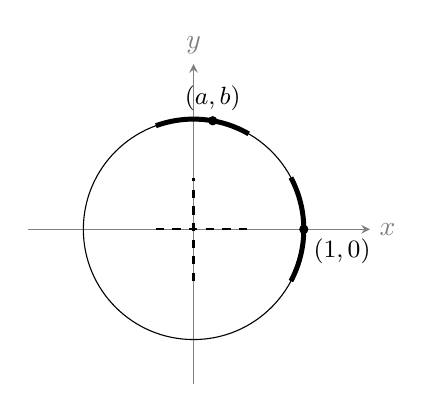
\begin{tikzpicture}[scale=1.4,>=stealth]
        \draw[gray,->] (-1.5,0)--(1.6,0) node[right] {$x$};
        \draw[gray,->] (0,-1.4)--(0,1.5) node[above] {$y$};
        \draw (0,0) circle (1);
        \draw[line width=1.8pt] (110:1) arc[start angle=110,end angle=60,radius=1];
        \fill (80:1) circle (1.2pt);
        \node[above] at (80:1) {\small $(a,b)$};
        \draw[thick,dashed] ({cos(110)},0)--({cos(60)},0);
        \draw[line width=1.8pt] (-28:1) arc[start angle=-28,end angle=28,radius=1];
        \fill (1,0) circle (1.2pt);
        \node[below right] at (1,0) {\small $(1,0)$};
        \draw[thick,dashed] (0,{sin(-28)})--(0,{sin(28)});
    \end{tikzpicture}
    \caption{Near $(a,b)$ with $b\neq0$, the circle is the graph of a function $y(x)$ over an interval of the $x$-axis (dashed). Near $(1,0)$ it is not, but it is the graph of a function $x(y)$ over an interval of the $y$-axis.}
    \label{fig implicit circle}
\end{figure}

\begin{thm}[\gls{immt}]\label{ImMT}\index{Theorem!Implicit mapping}
    Let $U\subset\bbR^n\times\bbR^k$ be open, $\varPhi\in C^\infty(U,\bbR^k)$, and let $(\bf{a},\bf{b})\in U$ satisfy $\varPhi(\bf{a},\bf{b})=\bf{c}$. If the $k\times k$ matrix $\big(\partial\varPhi^i/\partial y^j(\bf{a},\bf{b})\big)$ is invertible, then there are open neighborhoods $V\ni\bf{a}$ in $\bbR^n$ and $W\ni\bf{b}$ in $\bbR^k$ and a smooth map $g:V\to W$ such that
    \[\text{for all }(\bf{x},\bf{y})\in V\times W:\qquad\varPhi(\bf{x},\bf{y})=\bf{c}\iff\bf{y}=g(\bf{x}).\]
\end{thm}
\begin{proof}
    The map $F(\bf{x},\bf{y})=(\bf{x},\varPhi(\bf{x},\bf{y}))$ has the block triangular derivative
    \[DF=\begin{pmatrix}\rmI_n&0\\ \partial\varPhi/\partial\bf{x}&\partial\varPhi/\partial\bf{y}\end{pmatrix},\]
    which is invertible at $(\bf{a},\bf{b})$. By the inverse mapping theorem, $F$ restricts to a diffeomorphism from a neighborhood of $(\bf{a},\bf{b})$, which we may take to be a product $V'\times W$, onto an open set $O$. Since $F$ preserves $\bf{x}$, its inverse has the form $F^{-1}(\bf{x},\bf{z})=(\bf{x},h(\bf{x},\bf{z}))$ with $h$ smooth. Let $V=\{\bf{x}\in V'\mid(\bf{x},\bf{c})\in O\}$, which is open, and $g(\bf{x})=h(\bf{x},\bf{c})$. For $(\bf{x},\bf{y})\in V\times W$, we have $\varPhi(\bf{x},\bf{y})=\bf{c}$ iff $F(\bf{x},\bf{y})=(\bf{x},\bf{c})$ iff $\bf{y}=g(\bf{x})$.
\end{proof}
In words: the equation $\varPhi(\bf{x},\bf{y})=\bf{c}$ can be locally solved for $\bf{y}=g(\bf{x})$ if the matrix $\partial\varPhi/\partial\bf{y}$ is invertible. Differentiating $\varPhi(\bf{x},g(\bf{x}))=\bf{c}$ gives the derivative of the solution, $Dg=-(\partial\varPhi/\partial\bf{y})^{-1}\,\partial\varPhi/\partial\bf{x}$.

The same trick of adding the ``missing'' coordinates to a map gives a normal form for all maps whose derivative has constant rank. Recall that the rank of a matrix is the dimension of its image.

\begin{thm}[Constant rank theorem]\label{thm constant rank Rn}\index{Theorem!Constant rank}
    Let $U\subset\bbR^m$ be open and $f\in C^\infty(U,\bbR^n)$ be such that $\rank Df(\bf{x})=r$ for all $\bf{x}$ in a neighborhood of $\bf{a}\in U$. Then there are diffeomorphisms $\varphi$ from a neighborhood of $\bf{a}$ onto an open subset of $\bbR^m$, and $\psi$ from a neighborhood of $f(\bf{a})$ onto an open subset of $\bbR^n$, such that
    \[\psi\circ f\circ\varphi^{-1}(x^1,\ldots,x^m)=(x^1,\ldots,x^r,0,\ldots,0).\]
\end{thm}
\begin{proof}
    After permuting coordinates in $\bbR^m$ and $\bbR^n$, we may assume that the upper left $r\times r$ block of $Df(\bf{a})$ is invertible. Write $\bf{x}=(\bf{u},\bf{v})\in\bbR^r\times\bbR^{m-r}$ and $f=(F,G)$ with $F$ the first $r$ components. The map $\varphi(\bf{u},\bf{v})=(F(\bf{u},\bf{v}),\bf{v})$ has invertible derivative at $\bf{a}$, so it is a local diffeomorphism near $\bf{a}$, and by construction $f\circ\varphi^{-1}(\bf{u},\bf{v})=(\bf{u},\wt G(\bf{u},\bf{v}))$ for some smooth $\wt G$. The derivative of this map,
    \[\begin{pmatrix}\rmI_r&0\\ \partial\wt G/\partial\bf{u}&\partial\wt G/\partial\bf{v}\end{pmatrix},\]
    has rank $r$ near $\varphi(\bf{a})$, which forces $\partial\wt G/\partial\bf{v}=0$. So, on a small ball, $\wt G(\bf{u},\bf{v})=\wt G(\bf{u})$ does not depend on $\bf{v}$. Finally, the map $\psi(\bf{s},\bf{t})=(\bf{s},\bf{t}-\wt G(\bf{s}))$ is a diffeomorphism near $f(\bf{a})$, with inverse $(\bf{s},\bf{t})\mapsto(\bf{s},\bf{t}+\wt G(\bf{s}))$, and $\psi\circ f\circ\varphi^{-1}(\bf{u},\bf{v})=(\bf{u},0)$.
\end{proof}

The hypothesis of constant rank cannot be dropped: the function $x\mapsto x^2$ has derivative of rank $1$ at $x\neq0$ and of rank $0$ at $x=0$, and no change of coordinates turns it into either $x\mapsto x$ or $x\mapsto0$ near $0$. In two cases, however, the rank is automatically constant near $\bf{a}$. If $\rank Df(\bf{a})$ is maximal, i.e., equals $r=\min(m,n)$, then it stays maximal nearby, since some $r\times r$ minor of $Df$ is nonzero at $\bf{a}$, hence also nearby (cf.\ Proposition~\ref{domain of maximal rank}). So the theorem applies, and it gives the two \emph{local normal forms}
\[\begin{aligned}
    (x^1,\ldots,x^m)&\mapsto(x^1,\ldots,x^m,0,\ldots,0)&&(m\leq n),\\
    (x^1,\ldots,x^m)&\mapsto(x^1,\ldots,x^n)&&(m\geq n).
\end{aligned}\]
Up to changes of coordinates, a map with injective derivative is the inclusion of a coordinate plane, and a map with surjective derivative is a coordinate projection.

As a first application, we can now justify the definition of the boundary of a smooth manifold.

\begin{prop}[Invariance of the boundary]\label{prop smooth invariance of boundary}\index{Invariance of the boundary}
    No point of a smooth manifold with boundary is both an interior point and a boundary point.
\end{prop}
\begin{proof}
    Suppose that $m$ lies in the domain of an interior chart $\varphi:U\to\bbR^n$ and of a boundary chart $\psi:V\to\wb\bbR^n_+$ with $\psi(m)\in\partial\wb\bbR^n_+$. The transition map $\tau=\psi\circ\varphi^{-1}$ is smooth on the open set $\varphi(U\cap V)$, and its inverse $\varphi\circ\psi^{-1}$ extends to a smooth map $\sigma$ on a neighborhood of $\psi(m)$ in $\bbR^n$. By the chain rule applied to $\sigma\circ\tau=\id$, the derivative of $\tau$ at $\varphi(m)$ is invertible. By the inverse mapping theorem, $\tau$ maps a neighborhood of $\varphi(m)$ onto an \emph{open} subset of $\bbR^n$ that contains $\psi(m)$. But this open set lies in $\wb\bbR^n_+$, while every neighborhood of $\psi(m)\in\partial\wb\bbR^n_+$ contains points with $x^n<0$.
\end{proof}

\begin{cor}\label{cor diffeomorphisms preserve boundary}
    If $f:M\to N$ is a diffeomorphism of manifolds with boundary, then $f(\partial M)=\partial N$, and $f$ restricts to a diffeomorphism $\mathring M\to\mathring N$.
\end{cor}
\begin{proof}
    Composing the charts of $N$ with $f$ gives charts of $M$, so $f$ maps interior points to interior points and boundary points to boundary points. By the proposition, these two classes do not overlap.
\end{proof}


\section{Partitions of unity}\label{sec partitions of unity}

Many objects on a manifold are easy to construct in a single chart, and the problem is to glue the local constructions into a global one. Analytic functions are useless for this purpose: an analytic function on $\bbR^n$ that vanishes on an open set vanishes everywhere. Smooth functions, on the other hand, can be switched on and off at will.

\begin{lem}[Bump functions]\label{lem smooth bumps}\index{Bump function}
    \begin{enumerate}
        \item The function $h(t)=\rme^{-1/t}$ for $t>0$, $h(t)=0$ for $t\leq0$, is smooth on $\bbR$.
        \item The function $s(t)=\frac{h(t)}{h(t)+h(1-t)}$ is smooth, with $s=0$ for $t\leq0$, $s=1$ for $t\geq1$, and $0<s<1$ in between.
        \item For $\bf{x}_0\in\bbR^n$ and $0<r_1<r_2$, the function $\eta(\bf{x})=s\Big(\frac{r_2-\lvert\bf{x}-\bf{x}_0\rvert}{r_2-r_1}\Big)$ is smooth, equal to $1$ on $\wb B_{r_1}(\bf{x}_0)$, and positive exactly on $B_{r_2}(\bf{x}_0)$.
    \end{enumerate}
\end{lem}
\begin{proof}
    (1) For $t>0$, induction shows that $h^{(k)}(t)=p_k(1/t)\rme^{-1/t}$ for a polynomial $p_k$. Since $\rme^{-1/t}$ decays faster than any power of $t$ as $t\to0^+$, all these derivatives tend to $0$. By induction on $k$, $h^{(k)}(0)=\lim_{t\to0}h^{(k-1)}(t)/t=0$, so $h$ has continuous derivatives of all orders. (2) The denominator never vanishes. (3) The function $\lvert\bf{x}-\bf{x}_0\rvert$ is smooth away from $\bf{x}_0$, and $\eta$ is constant near $\bf{x}_0$.
\end{proof}
All derivatives of $h$ vanish at $0$, so its Taylor series at $0$ is zero, although $h$ is not. This is exactly what an analytic function cannot do (Figure~\ref{fig bump functions}).

\begin{figure}[tp]
    \centering
    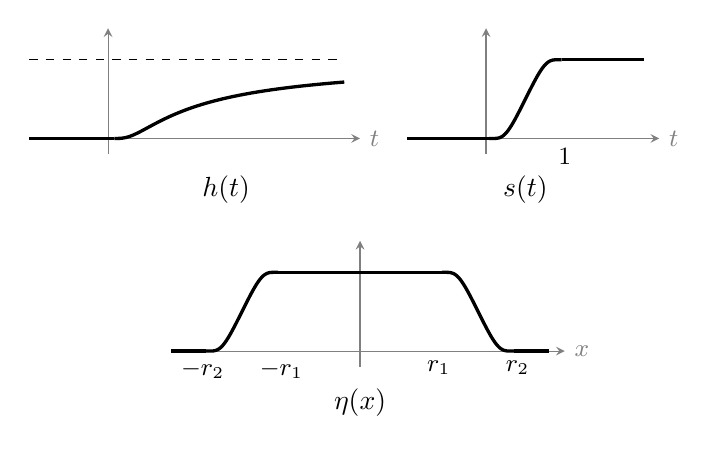
\begin{tikzpicture}[scale=1.0,>=stealth]
        \begin{scope}
            \draw[gray,->] (-1,0)--(3.2,0) node[right] {\small $t$};
            \draw[gray,->] (0,-0.2)--(0,1.4);
            \draw[very thick] (-1,0)--(0.08,0);
            \draw[very thick,domain=0.08:3,samples=80] plot (\x,{exp(-1/\x)});
            \draw[dashed] (-1,1)--(3,1);
            \node at (1.5,-0.65) {$h(t)$};
        \end{scope}
        \begin{scope}[xshift=4.8cm]
            \draw[gray,->] (-1,0)--(2.2,0) node[right] {\small $t$};
            \draw[gray,->] (0,-0.2)--(0,1.4);
            \draw[very thick] (-1,0)--(0.04,0);
            \draw[very thick,domain=0.04:0.96,samples=80] plot (\x,{exp(-1/\x)/(exp(-1/\x)+exp(-1/(1-\x)))});
            \draw[very thick] (0.96,1)--(2,1);
            \node[below] at (1,0) {\small $1$};
            \node at (0.5,-0.65) {$s(t)$};
        \end{scope}
        \begin{scope}[xshift=3.2cm,yshift=-2.7cm]
            \draw[gray,->] (-2.4,0)--(2.6,0) node[right] {\small $x$};
            \draw[gray,->] (0,-0.2)--(0,1.4);
            \draw[very thick] (-2.4,0)--(-1.96,0);
            \draw[very thick,domain=-1.96:-1.04,samples=60] plot (\x,{exp(-1/(2+\x))/(exp(-1/(2+\x))+exp(-1/(-1-\x)))});
            \draw[very thick] (-1.04,1)--(1.04,1);
            \draw[very thick,domain=1.04:1.96,samples=60] plot (\x,{exp(-1/(2-\x))/(exp(-1/(2-\x))+exp(-1/(\x-1)))});
            \draw[very thick] (1.96,0)--(2.4,0);
            \foreach \x/\l in {-2/-r_2,-1/-r_1,1/r_1,2/r_2} \node[below] at (\x,0) {\small $\l$};
            \node at (0,-0.65) {$\eta(x)$};
        \end{scope}
    \end{tikzpicture}
    \caption{The function $h(t)=\rme^{-1/t}$ (top left) is so flat at $0$ that it can be glued to the zero function smoothly. From it, we build a smooth step $s$ (top right) and a bump $\eta$ (bottom) that equals $1$ on $[-r_1,r_1]$ and vanishes outside $(-r_2,r_2)$.}
    \label{fig bump functions}
\end{figure}

\begin{xca}
    Construct a smooth function $f:\bbR\to\bbR$ that vanishes outside $(a,b)$ and is positive on $(a,b)$, using $\rme^{-1/((x-a)(b-x))}$. Use it to give another construction of the step function $s$.
\end{xca}

The \emph{support} of a function $f:X\to\bbR$ is the closed set $\supp f=\wb{\{x\mid f(x)\neq0\}}$.\index{Support of a function}

\begin{defn}[Partition of unity]\index{Partition of unity}
    A (smooth) \gls{pou} on a manifold $M$ is a collection of smooth functions $\chi_\alpha:M\to[0,1]$ such that the supports $\{\supp\chi_\alpha\}$ form a locally finite collection and $\sum_\alpha\chi_\alpha=1$. It is \emph{subordinate} to an open cover $\{U_\alpha\}$, indexed by the same set, if $\supp\chi_\alpha\subset U_\alpha$ for all $\alpha$.
\end{defn}
By local finiteness, each point has a neighborhood on which all but finitely many $\chi_\alpha$ vanish, so the sum is finite there. A \gls{pou} is a way to break the constant function $1$ into pieces supported in the given open sets (Figure~\ref{fig partition of unity}). Any function $f$ can then be broken into the pieces $\chi_\alpha f$, and conversely, any functions $f_\alpha$ defined on $U_\alpha$ can be glued into the function $\sum_\alpha\chi_\alpha f_\alpha$ on all of $M$, where $\chi_\alpha f_\alpha$ is extended by zero outside $U_\alpha$.

\begin{figure}[tp]
    \centering
    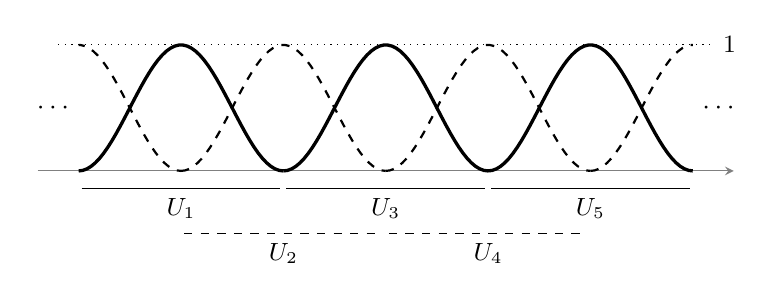
\begin{tikzpicture}[xscale=1.3,yscale=1.6,>=stealth]
        \draw[gray,->] (-0.4,0)--(6.4,0) node[right] {$\bbR$};
        \draw[dotted] (-0.2,1)--(6.2,1) node[right] {\small $1$};
        \begin{scope}
            \clip (0,-0.05) rectangle (6,1.1);
            \foreach \k in {1,3,5} \draw[very thick,domain={\k-1}:{\k+1},samples=50] plot (\x,{cos(90*(\x-\k))^2});
            \foreach \k in {0,2,4,6} \draw[thick,dashed,domain={\k-1}:{\k+1},samples=50] plot (\x,{cos(90*(\x-\k))^2});
        \end{scope}
        \node at (-0.25,0.5) {$\cdots$}; \node at (6.25,0.5) {$\cdots$};
        \foreach \k in {1,3,5} {
            \draw ({\k-0.97},-0.14)--({\k+0.97},-0.14);
            \node[below] at (\k,-0.14) {\small $U_\k$};
        }
        \foreach \k in {2,4} {
            \draw[dashed] ({\k-0.97},-0.5)--({\k+0.97},-0.5);
            \node[below] at (\k,-0.5) {\small $U_\k$};
        }
    \end{tikzpicture}
    \caption{A \gls{pou} on $\bbR$ (alternately solid and dashed graphs) subordinate to the cover by the intervals $U_k=(k-1,k+1)$, $k\in\bbZ$. At every point, at most two of the functions are nonzero, and their sum is $1$.}
    \label{fig partition of unity}
\end{figure}

To construct partitions of unity, we need the following observation about locally finite collections.

\begin{lem}\label{lem locally finite closure}\index{Locally finite collection}
    If $\{A_\beta\}$ is a locally finite collection of subsets of a space $X$, then $\wb{\bigcup_\beta A_\beta}=\bigcup_\beta\wb{A_\beta}$. In particular, a locally finite union of closed sets is closed.
\end{lem}
\begin{proof}
    The inclusion $\supset$ is clear. If $x\notin\bigcup_\beta\wb{A_\beta}$, then $x$ has a neighborhood $W$ that meets only finitely many sets $A_1,\ldots,A_k$, and $W\setminus(\wb{A_1}\cup\ldots\cup\wb{A_k})$ is a neighborhood of $x$ disjoint from all $A_\beta$.
\end{proof}

\begin{thm}[Existence of partitions of unity {{\cite[Prop.~1.3.7]{RS1}}}]\label{prop 1.3.7 RS1}
    Every open cover $\{U_\alpha\}$ of a smooth manifold $M$ has a subordinate smooth \gls{pou}.
\end{thm}
\begin{proof}
    \emph{Step 1: a good cover by balls.} Run the proof of Theorem~\ref{thm properties of manifolds}(c) with smooth charts, but cover each compact shell by the concentric balls of half the radius. We obtain a countable, locally finite collection of regular coordinate balls $\varphi_i:B_i\to B_{r_i}(\bf{q}_i)$, each contained in some $U_{a(i)}$, such that the smaller balls $B_i'=\varphi_i^{-1}(B_{r_i/2}(\bf{q}_i))$ still cover $M$.

    \emph{Step 2: bumps.} Let $\eta_i$ be the bump function of Lemma~\ref{lem smooth bumps} that equals $1$ on $\wb B_{r_i/2}(\bf{q}_i)$ and is supported in $\wb B_{3r_i/4}(\bf{q}_i)$. The function $\psi_i=\eta_i\circ\varphi_i$, extended by zero outside $B_i$, is smooth: it is smooth on $B_i$ and vanishes on the complement of the compact set $\varphi_i^{-1}(\wb B_{3r_i/4}(\bf{q}_i))$, and these two open sets cover $M$. The supports of the $\psi_i$ are locally finite, so $\psi=\sum_i\psi_i$ is smooth, and $\psi\geq1$, because every point lies in some $B_i'$.

    \emph{Step 3: normalization and regrouping.} The functions $\psi_i/\psi$ have sum $1$. Finally, put $\chi_\alpha=\sum_{i:\,a(i)=\alpha}\psi_i/\psi$. These functions are smooth and have sum $1$, and by Lemma~\ref{lem locally finite closure}, $\supp\chi_\alpha=\bigcup_{a(i)=\alpha}\supp\psi_i\subset U_\alpha$. Their supports are locally finite, because those of the $\psi_i$ are.
\end{proof}

Second countability entered this proof through the compact exhaustion, but only to obtain a locally finite refinement by coordinate balls. So the theorem holds for all paracompact Hausdorff smooth ``manifolds'', i.e., by Proposition~\ref{prop paracompact vs second countable}, for those whose components are second countable, such as the uncountable union of lines. Conversely, if every open cover has a subordinate \gls{pou}, then the sets $\{\chi_\alpha>0\}$ form a locally finite refinement, so the space is paracompact. Thus, for a Hausdorff space with a smooth atlas, paracompactness is equivalent to the existence of smooth partitions of unity. The same construction works on topological spaces once the Urysohn lemma replaces the bump functions, and paracompactness replaces the exhaustion.

\begin{thm}[{{\cite[Thm.~4.85]{LeeTop}}}]\label{thm continuous pou}
    Let $X$ be a paracompact Hausdorff space. Then
    \begin{enumerate}
        \item $X$ is normal;
        \item every open cover of $X$ has a subordinate continuous \gls{pou} (defined as above, with continuous functions).
    \end{enumerate}
\end{thm}
\begin{proof}
    (1) First we show that $X$ is regular. Let $A$ be closed and $x\notin A$. Every $a\in A$ has an open neighborhood $U_a$ with $x\notin\wb{U_a}$, by the Hausdorff property. Take a locally finite refinement of the cover $\{U_a\}_{a\in A}\cup\{X\setminus A\}$, and let $W$ be the union of its members that meet $A$. Each of them lies in some $U_a$, so its closure does not contain $x$. By Lemma~\ref{lem locally finite closure}, $x\notin\wb W$, so $W$ and $X\setminus\wb W$ separate $A$ and $x$. Repeating the argument with $x$ replaced by a closed set disjoint from $A$, and the Hausdorff property replaced by regularity, shows that $X$ is normal.

    (2) Let $\{V_\beta\}$ be a locally finite refinement of the cover. By regularity, every point has an open neighborhood whose closure lies in some $V_\beta$. A locally finite refinement $\{W_\gamma\}$ of the cover by these neighborhoods has the same property; assign to each $\gamma$ one such $\beta$. Then the sets $F_\beta=\bigcup\{\wb{W_\gamma}\mid\gamma\text{ assigned to }\beta\}$ are closed by Lemma~\ref{lem locally finite closure}, and they cover $X$, with $F_\beta\subset V_\beta$. By normality, choose open sets $V_\beta'$ with $F_\beta\subset V'_\beta\subset\wb{V_\beta'}\subset V_\beta$, and by the Urysohn lemma (Theorem~\ref{thm Urysohn lemma}), continuous functions $f_\beta:X\to[0,1]$ that equal $1$ on $F_\beta$ and $0$ outside $V'_\beta$. Now normalize and regroup exactly as in Step~3 above.
\end{proof}

Here are the first applications. In each of them, a local construction is globalized by a \gls{pou}.

\begin{cor}[Smooth Urysohn lemma]\label{cor smooth Urysohn}\index{Lemma!Urysohn!smooth}
    If $A$ and $B$ are disjoint closed subsets of a manifold $M$, there is a smooth function $f:M\to[0,1]$ with $\restr{f}{A}=0$ and $\restr{f}{B}=1$.
\end{cor}
\begin{proof}
    Take a \gls{pou} $\{\chi_0,\chi_1\}$ subordinate to the cover $\{M\setminus B,M\setminus A\}$, and let $f=\chi_1$. It vanishes on $A$, and $\chi_0$ vanishes on $B$, so $f=1-\chi_0=1$ there.
\end{proof}
Compare this with the continuous Urysohn lemma (Theorem~\ref{thm Urysohn lemma}): its proof had to build the function level set by level set, while here the bump functions do all the work. In particular, manifolds are normal. Manifolds are also metrizable (Proposition~\ref{prop paracompact vs second countable}); we will construct explicit metrics using Riemannian metrics in \Chap~\ref{ch riemannian geom}.

\begin{cor}\label{cor smooth functions determine topology}
    The topology of a manifold $M$ is the initial topology for the family of all smooth functions $f:M\to\bbR$.
\end{cor}
\begin{proof}
    Smooth functions are continuous, so the initial topology is coarser. Conversely, if $U$ is open and $x\in U$, then by Corollary~\ref{cor smooth Urysohn} there is a smooth $f$ with $f(x)=1$ and $f=0$ outside $U$, and $f^{-1}((0,\infty))$ is a neighborhood of $x$ in the initial topology that lies in $U$.
\end{proof}

\begin{rem}
    In fact, the algebra $C^\infty(M)$ remembers much more than the topology: a compact manifold can be recovered from it, with its points corresponding to the algebra homomorphisms $C^\infty(M)\to\bbR$ (see the following exercise). This is the smooth analog of the Gelfand duality of Example~\ref{example Gelfand duality}, and it is the starting point of algebraic approaches to geometry.
\end{rem}

\begin{xca}
    Let $M$ be a compact manifold and $\theta:C^\infty(M)\to\bbR$ a homomorphism of unital algebras. Show that $\theta$ is the evaluation at some point $m\in M$. \emph{Hint:} if not, for every $m$ there is $f_m$ with $\theta(f_m)=0$ and $f_m(m)\neq0$; use compactness to build a function $f=\sum_kf_{m_k}^2>0$ with $\theta(f)=0$.
\end{xca}

As for subsets of $\bbR^n$ in \S\ref{sec inverse function theorem}, a function $f$ on an arbitrary subset $A\subset M$ is \emph{smooth} if each point of $A$ has a neighborhood $W$ in $M$ and a smooth function on $W$ that agrees with $f$ on $A\cap W$.

\begin{thm}[Extension lemma]\label{extension lemma}\index{Extension lemma}
    Let $A\subset M$ be closed and $f:A\to\bbR^k$ smooth. Then for every open $U\supset A$ there is a smooth $\wt f:M\to\bbR^k$ with $\restr{\wt f}{A}=f$ and $\supp\wt f\subset U$.
\end{thm}
\begin{proof}
    For each $p\in A$, choose an open neighborhood $W_p\subset U$ and a smooth extension $f_p$ of $f$ to $W_p$. Let $\{\chi_p\}_{p\in A}\cup\{\chi_0\}$ be a \gls{pou} subordinate to the open cover $\{W_p\}_{p\in A}\cup\{M\setminus A\}$, and set $\wt f=\sum_{p\in A}\chi_pf_p$, where each term is extended by zero outside $W_p$. On $A$, we have $\chi_0=0$, so $\wt f=\sum_p\chi_pf=f$. The support of $\wt f$ lies in $\bigcup_p\supp\chi_p$, which is closed by Lemma~\ref{lem locally finite closure} and contained in $U$.
\end{proof}
The assumption that $A$ is closed is necessary: the function $1/x$ is smooth on $(0,\infty)\subset\bbR$, but it does not even have a continuous extension to $\bbR$.

\begin{defn}[Exhaustion function]\index{Exhaustion function}
    A continuous function $f:M\to\bbR$ is an \emph{exhaustion function} if all its sublevel sets $f^{-1}((-\infty,c])$ are compact.
\end{defn}
In other words, it is a proper function (\S\ref{sec: compactness}) that is bounded below. For example, $\lvert\bf{x}\rvert^2$ is an exhaustion function on $\bbR^n$, and every function on a compact manifold is one. An exhaustion function ``goes to infinity at the ends'' of $M$.

\begin{prop}\label{prop.exhaustion}
    Every manifold has a smooth exhaustion function.
\end{prop}
\begin{proof}
    Let $\{V_i\}_{i\in\bbN}$ be a countable cover of $M$ by precompact open sets (Theorem~\ref{thm properties of manifolds}), $\{\chi_i\}$ a subordinate \gls{pou}, and $f=\sum_ii\,\chi_i$. If $x\notin V_1\cup\ldots\cup V_N$, then $\chi_i(x)=0$ for $i\leq N$, so $f(x)=\sum_{i>N}i\,\chi_i(x)\geq N+1$. Thus $f^{-1}((-\infty,N])$ is a closed subset of the compact set $\wb{V_1}\cup\ldots\cup\wb{V_N}$.
\end{proof}

Finally, the zero sets of smooth functions turn out to be completely arbitrary closed sets. So, without further assumptions, the level sets of smooth functions can be very far from manifolds.

\begin{thm}\label{thm closed sets are zero sets}\index{Zero set}
    Every closed subset $K$ of a manifold $M$ is the zero set $f^{-1}(0)$ of a smooth function $f:M\to[0,1]$.
\end{thm}
\begin{proof}
    For $M=\bbR^n$, write the open set $\bbR^n\setminus K$ as a countable union of balls $B_i=B_{r_i}(\bf{q}_i)$, and let $\psi_i(\bf{x})=h(r_i^2-\lvert\bf{x}-\bf{q}_i\rvert^2)$, which is smooth, positive on $B_i$ and zero elsewhere. Choose constants $0<c_i\leq2^{-i}$ so small that all partial derivatives of $c_i\psi_i$ of order at most $i$ are bounded by $2^{-i}$. Then the series $f=\sum_ic_i\psi_i$ and all its termwise derivatives converge uniformly, so $f$ is smooth, and $f>0$ exactly on $\bbR^n\setminus K$. For a general manifold, apply this in charts and glue the results by a \gls{pou} (Exercise~\ref{xca zero sets on manifolds}).
\end{proof}

\begin{xca}\label{xca zero sets on manifolds}
    Complete the proof of the theorem for manifolds. \emph{Hint:} use a countable cover by charts $\varphi_j:V_j\to\bbR^n$ (onto all of $\bbR^n$), a subordinate \gls{pou} $\{\chi_j\}$, functions $f_j$ on $\bbR^n$ with zero sets $\varphi_j(K\cap V_j)$, and the sum $\sum_j\chi_j\cdot(f_j\circ\varphi_j)$.
\end{xca}

For example, the Cantor set is the zero set of a smooth function on $\bbR$. This shows why, in \S\ref{sec submanifolds}, only the level sets of \emph{regular} values are guaranteed to be manifolds. Partitions of unity will be used constantly later on, for instance, to construct Riemannian and bundle metrics (Theorem~\ref{prop 4.4.2 RS1}) and to define integrals of differential forms.


\section{Tangent spaces}\label{sec tangent spaces}

For a surface in $\bbR^3$, the tangent plane at a point $m$ consists of the velocity vectors of all curves through $m$ (Figure~\ref{fig tangent plane}). An abstract manifold is not contained in any ambient space where such vectors could live, and on a manifold, unlike in $\bbR^n$, vectors at different points cannot be compared without additional structure. So we must attach a separate vector space to every point, and define it intrinsically. There are three standard ways to do this: through curves, through derivatives of functions, and through coordinates. All three are useful, and we will show that they agree.

\begin{figure}[tp]
    \centering
    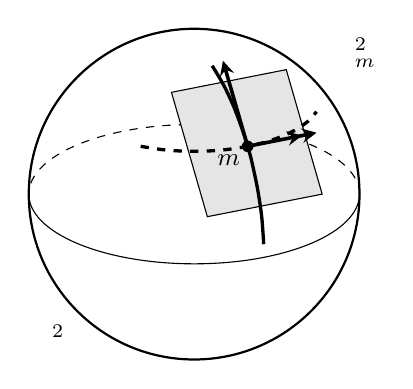
\begin{tikzpicture}[scale=1.5,>=stealth]
        \draw[thick] (0,0) circle (1.4);
        \draw (-1.4,0) arc[start angle=180,end angle=360,x radius=1.4,y radius=0.59];
        \draw[dashed] (1.4,0) arc[start angle=0,end angle=180,x radius=1.4,y radius=0.59];
        \fill[gray!20] (0.112,-0.191)--(1.084,0.000)--(0.780,1.054)--(-0.192,0.862)--cycle;
        \draw (0.112,-0.191)--(1.084,0.000)--(0.780,1.054)--(-0.192,0.862)--cycle;
        \draw[very thick] plot[smooth] coordinates {(0.589,-0.424) (0.572,-0.190) (0.536,0.050) (0.485,0.289) (0.453,0.405) (0.418,0.518) (0.339,0.732) (0.250,0.923) (0.153,1.087)};
        \draw[very thick,dashed] plot[smooth] coordinates {(-0.453,0.405) (-0.278,0.378) (-0.093,0.364) (0.093,0.364) (0.278,0.378) (0.453,0.405) (0.615,0.444) (0.758,0.495) (0.879,0.556) (0.972,0.624) (1.036,0.698)};
        \draw[->,line width=1.3pt] (0.453,0.405)--(0.244,1.129);
        \draw[->>,line width=1.3pt] (0.453,0.405)--(1.036,0.520);
        \fill (0.453,0.405) circle (1.4pt);
        \node[below left] at (0.47,0.42) {\small $m$};
        \node at (1.45,1.2) {$\T_m\bbS^2$};
        \node at (-1.15,-1.2) {$\bbS^2$};
    \end{tikzpicture}
    \caption{Two curves through $m$ on the sphere (solid and dashed) and their velocity vectors (single and double arrow), which span the tangent plane $\T_m\bbS^2$ (shaded).}
    \label{fig tangent plane}
\end{figure}

Let $M$ be an $n$-manifold and $m\in M$. By a \emph{curve through $m$} we mean a smooth map $\gamma:(-\epsilon,\epsilon)\to M$ with $\gamma(0)=m$.

\begin{defn}[Tangent vectors I: velocities]\index{Tangent vector}\index{Vector}
    Two curves $\gamma_1,\gamma_2$ through $m$ are \emph{tangent at $m$} if $(\varphi\circ\gamma_1)'(0)=(\varphi\circ\gamma_2)'(0)$ for some chart $\varphi$ around $m$. A \emph{tangent vector} at $m$ is an equivalence class $[\gamma]_m$ of tangent curves. The set of all tangent vectors at $m$ is the \emph{tangent space}\index{Tangent space} $\T_mM$.
\end{defn}
If $\psi$ is another chart, then by the chain rule $(\psi\circ\gamma)'(0)=D(\psi\circ\varphi^{-1})\big(\varphi(m)\big)(\varphi\circ\gamma)'(0)$, so the condition does not depend on the chart. For the same reason, the map
\[\varphi_{\ast m}:\T_mM\to\bbR^n,\qquad[\gamma]_m\mapsto(\varphi\circ\gamma)'(0),\]
is a bijection (the inverse sends $\bf{v}$ to the class of the curve $t\mapsto\varphi^{-1}(\varphi(m)+t\bf{v})$), and two such bijections differ by an invertible linear map, the Jacobi matrix of the transition map. So the vector space structure of $\bbR^n$ transported to $\T_mM$ by $\varphi_{\ast m}$ does not depend on $\varphi$, and $\dim\T_mM=\dim M$. For a boundary point $m\in\partial M$, we also allow curves defined on $[0,\epsilon)$ and $(-\epsilon,0]$; their velocities fill $\bbR^n$, and everything else goes through unchanged.

The second definition is based on the idea that a tangent vector is something that differentiates functions.

\begin{defn}[Tangent vectors II: derivations]\index{Derivation}
    A \emph{derivation at $m$} is a linear map $v:C^\infty(M)\to\bbR$ satisfying the Leibniz rule $v[fg]=f(m)v[g]+g(m)v[f]$.
\end{defn}
The derivations at $m$ obviously form a vector space. Every curve through $m$ gives a derivation, the \emph{directional derivative}\index{Directional derivative} $v_\gamma[f]=(f\circ\gamma)'(0)$, and two derivations agree if they come from tangent curves. In the other direction, we need the following lemma.

\begin{lem}[Hadamard]\label{lem Hadamard}\index{Lemma!Hadamard}
    Let $f$ be smooth on a ball $B\subset\bbR^n$ centered at $\bf{a}$. Then there are smooth functions $g_i$ on $B$ with $g_i(\bf{a})=\frac{\partial f}{\partial x^i}(\bf{a})$ and
    \[f(\bf{x})=f(\bf{a})+\sum_i(x^i-a^i)g_i(\bf{x}).\]
\end{lem}
\begin{proof}
    $f(\bf{x})-f(\bf{a})=\int_0^1\frac{\dd}{\dd t}f(\bf{a}+t(\bf{x}-\bf{a}))\dd t=\sum_i(x^i-a^i)\int_0^1\frac{\partial f}{\partial x^i}(\bf{a}+t(\bf{x}-\bf{a}))\dd t$.
\end{proof}

\begin{prop}
    The map $[\gamma]_m\mapsto v_\gamma$ is a linear isomorphism from $\T_mM$ onto the space of derivations at $m$.
\end{prop}
\begin{proof}
    In a chart $\varphi$, the chain rule gives $v_\gamma[f]=\sum_i\frac{\partial(f\circ\varphi^{-1})}{\partial x^i}(\varphi(m))\,v^i$, where $\bf{v}=\varphi_{\ast m}[\gamma]_m$. So the map is linear, and it is injective, since $v_\gamma$ applied to the coordinate functions $x^i$ recovers $\bf{v}$. (The functions $x^i$ are only defined near $m$, but we can multiply them by a bump function that equals $1$ near $m$ to make them global.)

    For surjectivity, first note two properties of a derivation $v$. It kills constants, since $v[1]=v[1\cdot1]=2v[1]$. It is \emph{local}: if $f=0$ near $m$, choose a bump function $\chi$ with $\chi(m)=1$ and $\chi f=0$; then $0=v[\chi f]=\chi(m)v[f]+f(m)v[\chi]=v[f]$. So $v$ can be applied to functions defined only near $m$. Now, let $v^i=v[x^i]$ and $\bf{a}=\varphi(m)$. By Hadamard's lemma, near $m$ we have $f=f(m)+\sum_i(x^i-a^i)\,(g_i\circ\varphi)$, and the Leibniz rule gives $v[f]=\sum_iv^ig_i(\bf{a})=\sum_iv^i\frac{\partial(f\circ\varphi^{-1})}{\partial x^i}(\bf{a})$, which is $v_\gamma[f]$ for the curve $\gamma$ with $\varphi_{\ast m}[\gamma]_m=\bf{v}$.
\end{proof}
The proof uses smoothness in an essential way. For functions of class $C^k$ with $k<\infty$, the functions $g_i$ in Hadamard's lemma are only of class $C^{k-1}$, and the space of derivations of $C^k(\bbR^n)$ at a point turns out to be infinite-dimensional. This is one of the reasons why smooth manifolds are more convenient than $C^k$ ones. From now on, we use both descriptions of tangent vectors interchangeably and write $X[f]$ for the derivative of $f$ along $X\in\T_mM$. Note that the second description does not need any modification at boundary points.

The third description is the one used by physicists: a tangent vector is a collection of components $\wh X^\alpha\in\bbR^n$, one for each chart $\varphi_\alpha$ around $m$, that transform by the Jacobi matrices of the transition maps when the chart changes. In our language, the components of $X_m\in\T_mM$ in the chart $\varphi_\alpha$ are
\[\wh X^\alpha_m\coloneqq\varphi_{\alpha\ast m}(X_m).\label{eq 1.4.8 RS1}\]
Since $\varphi_\beta=\varphi_{\beta\alpha}\circ\varphi_\alpha$ near $m$, the chain rule gives
\[\varphi_{\beta\ast m}=\left(\varphi_{\beta\alpha}\right)_{\ast\varphi_\alpha(m)}\circ\varphi_{\alpha\ast m},\label{eq 1.4.5 RS1}\]
where $\left(\varphi_{\beta\alpha}\right)_{\ast\varphi_\alpha(m)}$ is the Jacobi matrix of the transition map $\varphi_{\beta\alpha}:\varphi_\alpha(U_{\alpha\beta})\to\varphi_\beta(U_{\alpha\beta})$ at $\varphi_\alpha(m)$. In components,
\[\wh X^{\beta,i}_m=\left[\left(\varphi_{\beta\alpha}\right)_{\ast\varphi_\alpha(m)}\right]^i_j\wh X^{\alpha,j}_m.\label{eq 1.4.9 RS1}\]
(In a fixed coordinate system, we will usually omit the chart label $\alpha$.) Conversely, any collection of vectors $\wh X^\alpha\in\bbR^n$ that satisfies \eqref{eq 1.4.9 RS1} defines a unique tangent vector.

\begin{defn}[Differential]\index{Push-forward}\index{Differential}
    Let $F\in C^\infty(M,N)$ and $m\in M$. The \emph{differential} (or \emph{push-forward}, or \emph{derivative}) of $F$ at $m$ is the map $F_{\ast m}:\T_mM\to\T_{F(m)}N$ defined by
    \[F_{\ast m}([\gamma]_m)=[F\circ\gamma]_{F(m)},\quad\text{or equivalently}\quad F_{\ast m}(X)[f]=X[f\circ F]\quad\text{for }f\in C^\infty(N).\]
\end{defn}
In charts $\varphi$ around $m$ and $\psi$ around $F(m)$, let $\wh F=\psi\circ F\circ\varphi^{-1}$ be the local representative. Then $\psi\circ F\circ\gamma=\wh F\circ(\varphi\circ\gamma)$, and the chain rule shows that the differential is given by the Jacobi matrix of the local representative:
\[\widehat{F_{\ast m}X}=D\wh F\big(\varphi(m)\big)\,\wh X.\label{eq differential in local coordinates}\]
For a chart map itself, $\varphi_{\ast m}$ is the isomorphism $\T_mM\to\bbR^n$ used above, where we identify $\T_{\bf{x}}\bbR^n=\bbR^n$.

\begin{thm}\label{prop of push-forwards}\index{Chain rule}
    Let $M\overset{f}{\to}N\overset{g}{\to}P$ be smooth maps and $m\in M$. Then
    \begin{enumerate}
        \item $f_{\ast m}:\T_mM\to\T_{f(m)}N$ is linear, and in local coordinates it is given by the Jacobi matrix of the local representative of $f$;
        \item $(g\circ f)_{\ast m}=g_{\ast f(m)}\circ f_{\ast m}$ (chain rule), and $(\id_M)_{\ast m}=\id_{\T_mM}$;
        \item if $f$ is a diffeomorphism, then $f_{\ast m}$ is invertible and $(f_{\ast m})^{-1}=(f^{-1})_{\ast f(m)}$;
        \item conversely, if $M$ and $N$ have no boundary and $f_{\ast m}$ is invertible, then $f$ is a diffeomorphism from a neighborhood of $m$ onto a neighborhood of $f(m)$;
        \item (4) fails at boundary points.
    \end{enumerate}
\end{thm}
\begin{proof}
    (1) and (2) follow from \eqref{eq differential in local coordinates} and the chain rule of calculus, or directly from the definition. (3) follows from (2) applied to $f^{-1}\circ f=\id$ and $f\circ f^{-1}=\id$. (4) is the inverse mapping theorem applied to the local representative. (5) The inclusion $i:\wb\bbR^n_+\hookrightarrow\bbR^n$ has $i_{\ast0}=\id$, but it is not a diffeomorphism onto a neighborhood of $0$, since its image is not open.
\end{proof}

In the language of \Chap~\ref{ch category I}, statement (2) says that taking tangent spaces is a covariant functor $\T:\mathsf{Man}^\infty_\bullet\to\mathsf{Vect}_\bbR$ from the category of pointed manifolds $(M,m)$, whose morphisms are the smooth maps $f:(M,m)\to(N,f(m))$, to vector spaces. It sends $(M,m)$ to $\T_mM$ and $f$ to $f_{\ast m}$. In particular, (3) is a special case of the fact that functors send isomorphisms to isomorphisms, which immediately implies that diffeomorphic manifolds have the same dimension.

\begin{example}\label{example tangent spaces}
    \begin{enumerate}
        \item For an open subset $U\subset\bbR^n$, and in particular for $\GL_n(\bbR)\subset\Mat_n(\bbR)$, we have $\T_{\bf{x}}U=\bbR^n$ (respectively, $\T_A\GL_n(\bbR)=\Mat_n(\bbR)$): the class of a curve is determined by its ordinary velocity.
        \item \emph{The sphere.}\index{Tangent space!of the sphere} The inclusion $\iota:\bbS^n\hookrightarrow\bbR^{n+1}$ has injective differential, since in a hemisphere chart its local representative $\bf{y}\mapsto(\bf{y},\sqrt{1-\lvert\bf{y}\rvert^2})$ has an injective Jacobi matrix. So we may regard $\T_{\bf{x}}\bbS^n$ as the $n$-dimensional subspace $\iota_\ast(\T_{\bf{x}}\bbS^n)\subset\bbR^{n+1}$, consisting of the velocities $\gamma'(0)$ of curves in the sphere. Differentiating $\lvert\gamma(t)\rvert^2=1$ at $t=0$ gives $\bf{x}\cdot\gamma'(0)=0$. By counting dimensions, $\T_{\bf{x}}\bbS^n=\bf{x}^\perp$, the tangent plane of Figure~\ref{fig tangent plane}.
    \end{enumerate}
\end{example}

As we will see in \S\ref{sec tangent bundle}, the tangent spaces $\T_mM$ in a certain sense ``vary smoothly with $m$'', and together they form a single manifold, the \emph{tangent bundle}\index{Tangent bundle}.


\section{Rank}\label{sec rank}

\begin{defn}[Rank of a map]\label{def.rank}\index{Rank!of a map}
    The \emph{rank} of a smooth map $f:M\to N$ at $m\in M$ is $\rank_mf=\rank f_{\ast m}=\dim f_{\ast m}(\T_mM)$. In charts, it is the rank of the Jacobi matrix of the local representative of $f$. The map has \emph{constant rank}\index{Rank!constant} $r$ if $\rank_mf=r$ for all $m\in M$.
\end{defn}
The constant rank theorem (Theorem~\ref{thm constant rank Rn}) immediately carries over from $\bbR^n$ to manifolds.

\begin{thm}[Rank theorem]\index{Rank theorem}\label{Rank thm}
    Let $M^m$ and $N^n$ be manifolds without boundary, and let $f\in C^\infty(M,N)$ have constant rank $r$ in a neighborhood of $m_0\in M$. Then there are charts $\varphi$ around $m_0$ and $\psi$ around $f(m_0)$ in which $f$ has the local representative
    \[\psi\circ f\circ\varphi^{-1}(x^1,\ldots,x^m)=(x^1,\ldots,x^r,0,\ldots,0).\]
\end{thm}
\begin{proof}
    Apply Theorem~\ref{thm constant rank Rn} to the local representative of $f$ in arbitrary charts, and compose these charts with the diffeomorphisms provided by that theorem.
\end{proof}

\begin{prop}\label{domain of maximal rank}
    For every $k$, the set $\{m\in M\mid\rank_mf\geq k\}$ is open. In particular, the set of points where the rank of $f$ is maximal, i.e., $\rank_mf=\min(\dim M,\dim N)$, is open in $M$.
\end{prop}
\begin{proof}
    The rank of the Jacobi matrix is at least $k$ iff some $k\times k$ minor is nonzero, and the minors are continuous functions of the point.
\end{proof}
In other words, the rank is lower semicontinuous: near a given point, it can only be larger or equal, and it can drop only in a limit. For example, the function $f(x,y)=xy$ on $\bbR^2$ has the Jacobi matrix $(y\;\;x)$, which has rank $1$ everywhere except at the origin, where it has rank $0$. The level sets of $f$ are hyperbolas, except the level set through the origin, which is a cross (compare Figure~\ref{fig level sets}).

If $\dim M\leq\dim N$, then the maximal possible rank is $\dim M$, and a linear map has this rank iff it is injective. If $\dim M\geq\dim N$, then the maximal possible rank is $\dim N$, and the maps of maximal rank are the surjective ones. Maps of maximal rank are of special significance.

\begin{defn}[Immersions and submersions]\label{def immersion submersion}\index{Immersion!smooth}\index{Submersion!smooth}\index{Local diffeomorphism}
    A smooth map $f:M\to N$ is
    \begin{enumerate}
        \item an \emph{immersion} if $f_{\ast m}$ is injective for all $m\in M$, i.e., $f$ has constant rank $\dim M$;
        \item a \emph{submersion} if $f_{\ast m}$ is surjective for all $m\in M$, i.e., $f$ has constant rank $\dim N$;
        \item a \emph{local diffeomorphism} if every point $m\in M$ has an open neighborhood $U$ such that $f(U)$ is open and $\restr{f}{U}:U\to f(U)$ is a diffeomorphism.
    \end{enumerate}
\end{defn}
By the inverse mapping theorem, a map between manifolds without boundary is a local diffeomorphism iff it is both an immersion and a submersion. By the rank theorem, an immersion looks locally like the inclusion $\bbR^m\hookrightarrow\bbR^n$ of a coordinate plane, and a submersion looks locally like the projection $\bbR^m\to\bbR^n$ onto the first coordinates. Here ``locally'' refers to both the domain and the target: we have to restrict to neighborhoods of both $m$ and $f(m)$. Maps that look like projections over entire open sets of the target are \emph{fiber bundles}, and they will be studied in \Chap~\ref{chap: Fiber bundles}. Surjective submersions are not necessarily fiber bundles.

\begin{example}\label{example rank}
    \begin{enumerate}
        \item A curve $\gamma:I\to M$ is an immersion iff its velocity never vanishes. The curve $t\mapsto(t^2,t^3)$ in $\bbR^2$ is not an immersion at $t=0$, which is where its image has a cusp (Figure~\ref{fig cusp}).
        \item A function $f:M\to\bbR$ is a submersion iff it has no critical points, i.e., $f_{\ast m}\neq0$ for all $m$. For example, $\lvert\bf{x}\rvert^2$ is a submersion on $\bbR^n\setminus\{0\}$.
        \item \emph{The determinant.}\index{Determinant!differential of} For $A\in\GL_n(\bbR)$ and $H\in\Mat_n(\bbR)$, we have $\det(A+tH)=\det A\,\det(\rmI_n+tA^{-1}H)$, and expanding the last determinant shows that $\det(\rmI_n+tB)=1+t\tr B+O(t^2)$. Thus
        \[\det\nolimits_{\ast A}(H)=\restr{\frac{\dd}{\dd t}}{t=0}\det(A+tH)=\det A\cdot\tr(A^{-1}H).\]
        Taking $H=A$ gives $\det\nolimits_{\ast A}(A)=n\det A\neq0$, so $\det:\GL_n(\bbR)\to\bbR$ is a submersion.
        \item \emph{Gram matrices.}\index{Gram matrix} Let $\Sym_n\subset\Mat_n(\bbR)$ be the space of symmetric matrices, of dimension $\frac{n(n+1)}2$, and let $F(A)=A^\top A$. Then $F_{\ast A}(H)=H^\top A+A^\top H$. If $A$ is invertible, every symmetric $S$ is of this form, with $H=\frac12(A^\top)^{-1}S$. So $F:\GL_n(\bbR)\to\Sym_n$ is a submersion.
    \end{enumerate}
\end{example}
We will use the last two examples in \S\ref{sec submanifolds} to show that the classical groups $\SL_n(\bbR)$ and $\Or_n$ are manifolds. The constant rank condition is surprisingly strong globally, as the following theorem shows.

\begin{thm}[Global rank theorem]\label{Global rank}\index{Rank theorem!global}
    Let $M$ and $N$ be manifolds without boundary, and let $f\in C^\infty(M,N)$ have constant rank $r$.
    \begin{enumerate}
        \item If $f$ is injective, then it is an immersion.
        \item If $f$ is surjective, then it is a submersion.
        \item If $f$ is bijective, then it is a diffeomorphism.
    \end{enumerate}
\end{thm}
\begin{proof}
    (1) If $r<\dim M$, then by the rank theorem, there are coordinates near any point in which $f$ does not depend on the last coordinate, so $f$ is not injective.

    (2) Suppose $r<n=\dim N$. By the rank theorem, every point of $M$ has a precompact neighborhood $U$ such that $f(\wb U)$ is a compact subset of an $r$-dimensional coordinate slice $\{y^{r+1}=\ldots=y^n=0\}$ of a chart of $N$. Such a set is closed and has empty interior in $N$, since an open subset of $\bbR^n$ cannot lie in $\bbR^r\times\{0\}$. By second countability, countably many such sets $\wb{U_i}$ cover $M$, so $N=\bigcup_if(\wb{U_i})$ is a countable union of closed sets with empty interiors. Then a closed coordinate ball $\wb B\subset N$, which is a complete metric space, is a countable union of the closed sets $\wb B\cap f(\wb{U_i})$ with empty interiors, contradicting the Baire category theorem (Theorem~\ref{thm Baire}).

    (3) By (1) and (2), $f$ is a bijective local diffeomorphism, so its inverse is smooth.
\end{proof}


\section{Sard's theorem}\label{sec Sard}

Most values of a smooth map are regular. To make this precise, we need a notion of ``smallness'' for subsets of manifolds. A set $A\subset\bbR^n$ has \emph{measure zero} if for every $\epsilon>0$ it can be covered by countably many cubes of total volume less than $\epsilon$.\index{Measure zero} In this definition, we may equally use rectangular boxes instead of cubes, since a box can be covered by finitely many small cubes of total volume at most twice its own. A countable union of sets of measure zero has measure zero (cover the $i$-th set with total volume $\epsilon/2^i$). A nonempty open set does not have measure zero, so sets of measure zero have empty interior.

\begin{lem}\label{lem C1 preserves measure zero}
    Let $U\subset\bbR^n$ be open and $F:U\to\bbR^n$ of class $C^1$. If $A\subset U$ has measure zero, then so does $F(A)$.
\end{lem}
\begin{proof}
    Cover $U$ by countably many closed balls $\wb B_r$ such that the concentric balls $\wb B_{2r}$ also lie in $U$; it suffices to treat $A\cap\wb B_r$ for one such ball. On $\wb B_{2r}$, $\lVert DF\rVert\leq L$ for some $L$. Cover $A\cap\wb B_r$ by cubes of total volume $\epsilon$. For small $\epsilon$, these cubes are so small that those meeting $\wb B_r$ lie in $\wb B_{2r}$. So by the mean value inequality, $F$ maps such a cube of side $s$ into a ball of radius $L\sqrt n\,s$, i.e., into a cube of volume $(2L\sqrt n)^ns^n$. Thus $F(A\cap\wb B_r)$ is covered by cubes of total volume at most $(2L\sqrt n)^n\epsilon$.
\end{proof}

\begin{defn}[Measure zero in manifolds]
    A subset $A$ of an $n$-manifold $M$ has \emph{measure zero} if $\varphi(A\cap U)$ has measure zero in $\bbR^n$ for every smooth chart $(U,\varphi)$.
\end{defn}
By the lemma, it suffices to check this for the charts of a single atlas, and by second countability, for countably many charts. There is no canonical way to measure volumes on a manifold, but sets of measure zero are well-defined. As a first example, lower-dimensional manifolds are small.

\begin{prop}\label{prop mini Sard}
    If $\dim M<\dim N$, then the image of every smooth map $f:M\to N$ has measure zero.
\end{prop}
\begin{proof}
    Let $m=\dim M$ and $n=\dim N$. Working in countably many charts, we may assume that $f:U\to\bbR^n$ with $U\subset\bbR^m$ open. The map $F(\bf{x},\bf{y})=f(\bf{x})$ on $U\times\bbR^{n-m}$ is smooth, and $f(U)=F(U\times\{0\})$ is the image of a set of measure zero in $\bbR^n$.
\end{proof}

Smoothness is essential here: there are continuous surjections $[0,1]\to[0,1]^2$, called \emph{space-filling curves}\index{Space-filling curve}. One of them, due to Hilbert, is the uniform limit of the polygonal curves in Figure~\ref{fig Hilbert curve}: each curve consists of four copies of the previous one, scaled by $\frac12$, suitably rotated or reflected, placed in the four quarters of the square, and joined by three segments.

\begin{figure}[tp]
    \centering
    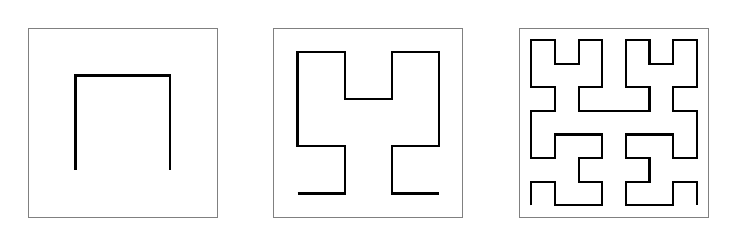
\begin{tikzpicture}[scale=1.2,>=stealth]
        \draw[gray] (0.0,0) rectangle (2.0,2);
        \draw[thick] (0.500,0.500) -- (0.500,1.500) -- (1.500,1.500) -- (1.500,0.500);
        \draw[gray] (2.6,0) rectangle (4.6,2);
        \draw[thick] (2.850,0.250) -- (3.350,0.250) -- (3.350,0.750) -- (2.850,0.750) -- (2.850,1.250) -- (2.850,1.750) -- (3.350,1.750) -- (3.350,1.250) -- (3.850,1.250) -- (3.850,1.750) -- (4.350,1.750) -- (4.350,1.250) -- (4.350,0.750) -- (3.850,0.750) -- (3.850,0.250) -- (4.350,0.250);
        \draw[gray] (5.2,0) rectangle (7.2,2);
        \draw[thick] (5.325,0.125) -- (5.325,0.375) -- (5.575,0.375) -- (5.575,0.125) -- (5.825,0.125) -- (6.075,0.125) -- (6.075,0.375) -- (5.825,0.375) -- (5.825,0.625) -- (6.075,0.625) -- (6.075,0.875) -- (5.825,0.875) -- (5.575,0.875) -- (5.575,0.625) -- (5.325,0.625) -- (5.325,0.875) -- (5.325,1.125) -- (5.575,1.125) -- (5.575,1.375) -- (5.325,1.375) -- (5.325,1.625) -- (5.325,1.875) -- (5.575,1.875) -- (5.575,1.625) -- (5.825,1.625) -- (5.825,1.875) -- (6.075,1.875) -- (6.075,1.625) -- (6.075,1.375) -- (5.825,1.375) -- (5.825,1.125) -- (6.075,1.125) -- (6.325,1.125) -- (6.575,1.125) -- (6.575,1.375) -- (6.325,1.375) -- (6.325,1.625) -- (6.325,1.875) -- (6.575,1.875) -- (6.575,1.625) -- (6.825,1.625) -- (6.825,1.875) -- (7.075,1.875) -- (7.075,1.625) -- (7.075,1.375) -- (6.825,1.375) -- (6.825,1.125) -- (7.075,1.125) -- (7.075,0.875) -- (7.075,0.625) -- (6.825,0.625) -- (6.825,0.875) -- (6.575,0.875) -- (6.325,0.875) -- (6.325,0.625) -- (6.575,0.625) -- (6.575,0.375) -- (6.325,0.375) -- (6.325,0.125) -- (6.575,0.125) -- (6.825,0.125) -- (6.825,0.375) -- (7.075,0.375) -- (7.075,0.125);
    \end{tikzpicture}
    \caption{The first three approximations of Hilbert's space-filling curve. They converge uniformly to a continuous surjection of the interval onto the square, so the smoothness assumption in Proposition~\ref{prop mini Sard} cannot be dropped.}
    \label{fig Hilbert curve}
\end{figure}

\begin{defn}[Critical and regular points and values]\index{Critical points/values}\index{Regular points/values}
    Let $f\in C^\infty(M,N)$. A point $m\in M$ is a \emph{critical point} of $f$ if $\rank_mf<\dim N$, i.e., if $f_{\ast m}$ is not surjective, and a \emph{regular point} otherwise. A \emph{critical value} is the image of a critical point, and all other points of $N$ are \emph{regular values}. Thus $q\in N$ is a regular value iff all points of $f^{-1}(q)$ are regular; in particular, points outside $f(M)$ are regular values.
\end{defn}

\begin{example}\label{example critical values}
    \begin{enumerate}
        \item The function $f(x)=x^3-3x$ has the critical points $x=\pm1$ and the critical values $\mp2$ (Figure~\ref{fig critical values}). A regular value $c$ has one preimage if $\lvert c\rvert>2$ and three preimages if $\lvert c\rvert<2$; the number of preimages changes only at the critical values.
        \item Consider the torus standing upright on a table, with the height function $h:\bbT^2\to\bbR$ (Figure~\ref{fig critical values}). It has four critical points: the minimum, the maximum, and two saddle points on the boundary of the hole. The level sets of regular values are one or two circles, while the level sets of the two saddle values are curves shaped like a figure eight.
        \item If $\dim M<\dim N$, then every point of $M$ is critical, and the set of critical values $f(M)$ has measure zero by Proposition~\ref{prop mini Sard}.
    \end{enumerate}
\end{example}

\begin{figure}[tp]
    \centering
    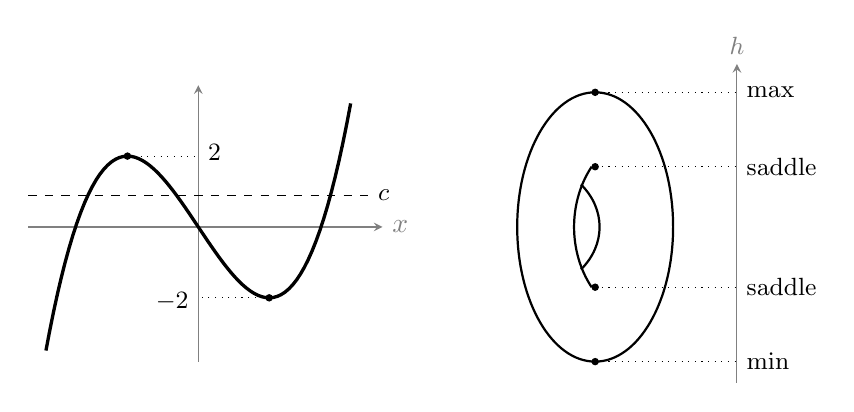
\begin{tikzpicture}[scale=0.9,>=stealth]
        \draw[gray,->] (-2.4,0)--(2.6,0) node[right] {$x$};
        \draw[gray,->] (0,-1.9)--(0,2.0);
        \draw[very thick,domain=-2.15:2.15,samples=80] plot (\x,{0.5*(\x*\x*\x-3*\x)});
        \draw[dotted] (-1,1)--(0,1) (1,-1)--(0,-1);
        \fill (-1,1) circle (1.5pt); \fill (1,-1) circle (1.5pt);
        \node[right] at (0,1.05) {\small $2$};
        \node[left] at (0,-1.05) {\small $-2$};
        \draw[dashed] (-2.4,0.45)--(2.4,0.45) node[right] {\small $c$};
        \begin{scope}[xshift=5.6cm]
            \draw[thick] (0,0) ellipse (1.1 and 1.9);
            \draw[thick] (-0.05,-0.85) .. controls (-0.38,-0.35) and (-0.38,0.35) .. (-0.05,0.85);
            \draw[thick] (-0.2,-0.6) .. controls (0.15,-0.25) and (0.15,0.25) .. (-0.2,0.6);
            \foreach \y in {-1.9,-0.85,0.85,1.9} {
                \fill (0,\y) circle (1.5pt);
                \draw[dotted] (0,\y)--(2.0,\y);
            }
            \draw[gray,->] (2.0,-2.2)--(2.0,2.3) node[above] {\small $h$};
            \node[right] at (2.0,-1.9) {\small min};
            \node[right] at (2.0,-0.85) {\small saddle};
            \node[right] at (2.0,0.85) {\small saddle};
            \node[right] at (2.0,1.9) {\small max};
        \end{scope}
    \end{tikzpicture}
    \caption{Left: the graph of $x^3-3x$ (vertical scale halved). The dashed horizontal line at a regular value $c$ meets the graph in three points; at the critical values $\pm2$, two of these points merge. Right: the height function on an upright torus has four critical points.}
    \label{fig critical values}
\end{figure}

For $\dim M<\dim N$, the following theorem says no more than Proposition~\ref{prop mini Sard}. In all other cases, we have to use the fact that the points in question are critical. For $\dim M=\dim N$, we will need the following classical covering lemma, which we do not prove (see, e.g., \href{https://en.wikipedia.org/wiki/Vitali_covering_lemma}{Vitali's covering lemma}).

\begin{lem}[Vitali]\label{lem Vitali}\index{Lemma!Vitali covering}
    Let $\mathcal{B}$ be a family of balls in $\bbR^m$ with bounded radii. Then there is a countable subfamily of pairwise disjoint balls $B_{r_i}(\bf{x}_i)\in\mathcal{B}$ such that the balls $B_{5r_i}(\bf{x}_i)$ cover all the balls of $\mathcal{B}$.
\end{lem}

\begin{thm}[Sard {{\cite[Thm.~6.10]{Lee}}}]\index{Theorem!Sard}\label{thm sard}
    The set of critical values of a smooth map $f:M\to N$ (also known in some contexts as the \emph{caustic} of $f$) has measure zero in $N$. In particular, the regular values of $f$ are dense in $N$.
\end{thm}
\begin{proof}[Proof for $\dim M\leq\dim N$]
    The theorem is local: every manifold is covered by countably many charts, and a countable union of sets of measure zero has measure zero. So let $f:U\to\bbR^n$ with $U\subset\bbR^m$ open and $m\leq n$, and let $C$ be the set of critical points. We split $C$ into the countably many pieces on which $\lVert Df\rVert\leq L$, $L\in\bbN$, and cover $U$ by countably many closed cubes $Q$. So it suffices to show that $f(A)$ has measure zero, where
    \[A=\{\bf{x}\in C\cap Q\mid\lVert Df(\bf{x})\rVert\leq L\}.\]

    Fix a large $p\in\bbN$ and $\bf{x}\in A$. The rank $k$ of $Df(\bf{x})$ is less than $n$, so $Df(\bf{x})$ maps the ball $B_r(0)$ into a $k$-dimensional disk of radius $Lr$. By differentiability, there is $\delta>0$ such that
    \[\lvert f(\bf{y})-f(\bf{x})-Df(\bf{x})(\bf{y}-\bf{x})\rvert\leq\frac1p\lvert\bf{y}-\bf{x}\rvert\quad\text{for all }\bf{y}\in B_\delta(\bf{x}).\]
    So if $r<\delta$, then $f(B_r(\bf{x}))$ lies within distance $r/p$ of a $k$-dimensional disk of radius $Lr$. Such a disk can be cut into at most $c\,p^k$ pieces of size $r/p$, where the constant $c$ depends only on $L$ and $n$. Hence $f(B_r(\bf{x}))$ can be covered by $c\,p^k$ cubes in $\bbR^n$ whose sides are proportional to $r/p$. Their total volume is at most a constant times
    \[p^k\Big(\frac rp\Big)^n\leq\frac{r^n}{p}\leq\frac{r^m}{p},\]
    where we used $k\leq n-1$, and also $r<1$ and $m\leq n$.

    Choose such a radius $r_{\bf{x}}<\min(\delta,1)$ for every $\bf{x}\in A$, small enough that $B_{r_{\bf{x}}}(\bf{x})\subset U$. By Vitali's covering lemma, applied to the balls $B_{r_{\bf{x}}/5}(\bf{x})$, there are countably many points $\bf{x}_i\in A$, with $r_i=r_{\bf{x}_i}$, such that the balls $B_{r_i}(\bf{x}_i)$ cover $A$, while the balls $B_{r_i/5}(\bf{x}_i)$ are pairwise disjoint. All of the latter lie in a fixed cube, obtained by enlarging $Q$, so the sum of their volumes is bounded by the volume of that cube. Hence $\sum_ir_i^m$ is bounded by a constant that does not depend on $p$. So $f(A)$ is covered by cubes of total volume at most a constant times $\sum_ir_i^m/p$, which tends to $0$ as $p\to\infty$.

    This proof is due to Behnam Esmayli.
\end{proof}
Notice that this argument only uses the differentiability of $f$ at each critical point separately. So for $\dim M\leq\dim N$, the theorem holds for all differentiable maps, even if their derivatives are not continuous. Vitali's lemma is what makes this possible, since it can handle balls whose radii vary wildly from point to point.

This is the heart of the matter: near a critical point, $f$ squashes a small ball into a thin neighborhood of a lower-dimensional disk. What happens when $m=\dim M$ is larger than $n=\dim N$? The image of each ball can still be covered by cubes of total volume about $r^n/p$. But the disjoint balls only give us control over the sum of the numbers $r_i^m$, and for $m>n$, the numbers $r_i^n$ are much larger. So the images of small balls have to be much smaller than before. This is the case at the points where many derivatives of $f$ vanish. At all other critical points, we can use one of the nonvanishing derivatives to lower the dimension by one. To put the lower-dimensional results back together, we need a simple version of Fubini's theorem.

\begin{lem}\label{lem Fubini measure zero}\index{Theorem!Fubini (for measure zero)}
    Let $A\subset\bbR^n$, $n\geq2$, be compact. If all of its slices $A_t=\{\bf{z}\in\bbR^{n-1}\mid(t,\bf{z})\in A\}$ have measure zero in $\bbR^{n-1}$, then $A$ has measure zero.
\end{lem}
\begin{proof}
    Let $A\subset[a,b]\times\bbR^{n-1}$ and $\epsilon>0$. For every $t\in[a,b]$, cover the compact set $A_t$ by finitely many open cubes of total volume less than $\epsilon$, and let $W_t$ be their union. There is an open interval $I_t\ni t$ such that $A_s\subset W_t$ for all $s\in I_t$: otherwise, there would be points $(s_i,\bf{z}_i)\in A$ with $s_i\to t$ and $\bf{z}_i\notin W_t$, and a limit point of this sequence would be a point $(t,\bf{z})\in A$ with $\bf{z}\notin W_t$. Finitely many of the intervals $I_t$ cover $[a,b]$, and discarding the redundant ones, we may assume that no point lies in three of them. Then the total length of the intervals $I_t\cap[a,b]$ is at most $2(b-a)$. So the products of these intervals with the cubes that make up $W_t$ are boxes of total volume at most $2(b-a)\epsilon$ that cover $A$.
\end{proof}

\begin{proof}[Proof of Sard's theorem in general]
    This argument follows \cite[\S3]{MilnorTDV}. As before, it suffices to consider a smooth map $f:U\to\bbR^n$, $n\geq1$, where $U\subset\bbR^m$ is open, and to show that $f(C)$ has measure zero, where $C$ is the set of critical points. We use induction on $m$, the case $m=0$ being trivial. Let $C_i\subset C$, $i\geq1$, be the set of points at which all partial derivatives of $f$ of orders $1,\ldots,i$ vanish. These sets are closed in $U$, and $C\supset C_1\supset C_2\supset\ldots$ So we can split $C$ into $C_k$, the layers $C_i\setminus C_{i+1}$ with $1\leq i<k$, and $C\setminus C_1$, where $k$ is chosen such that $(k+1)n>m$.

    \emph{Very flat points: $C_k$.} Here the images are so small that we can simply count the cubes of a uniform grid. Let $Q\subset U$ be a closed cube of side $\ell$, divided into $p^m$ subcubes. For $\bf{x}\in C_k\cap Q$ and $\bf{y}\in Q$, Taylor's theorem gives $\lvert f(\bf{y})-f(\bf{x})\rvert\leq c\lvert\bf{y}-\bf{x}\rvert^{k+1}$ for a constant $c$. So the image of a subcube that meets $C_k$ lies in a cube of side $2c(\sqrt m\,\ell/p)^{k+1}$. The total volume of these cubes is at most a constant times $p^{m-(k+1)n}$, which tends to $0$ as $p\to\infty$. Countably many cubes $Q$ cover $U$.

    \emph{Intermediate layers: $C_i\setminus C_{i+1}$.} Near a point $\bf{a}$ of such a layer, there is a partial derivative $w$ of order $i$ of some component of $f$ that vanishes on $C_i$, but has, say, $\partial w/\partial x^1(\bf{a})\neq0$. Then $h(\bf{x})=(w(\bf{x}),x^2,\ldots,x^m)$ is a diffeomorphism from a neighborhood $V$ of $\bf{a}$ onto an open set, and it maps $C_i\cap V$ into the hyperplane $\{0\}\times\bbR^{m-1}$. Let $\wb g$ be the restriction of $f\circ h^{-1}$ to this hyperplane. The derivative of $\wb g$ vanishes at all points of $h(C_i\cap V)$, because $Df$ vanishes on $C_i$. So these are critical points of $\wb g$, and by induction, $f(C_i\cap V)$ has measure zero. Countably many such neighborhoods $V$ cover the layer.

    \emph{The remaining points: $C\setminus C_1$.} For $n=1$, there are no such points, so let $n\geq2$. Near a point $\bf{a}\in C\setminus C_1$, we may assume that $\partial f^1/\partial x^1(\bf{a})\neq0$. Then $h(\bf{x})=(f^1(\bf{x}),x^2,\ldots,x^m)$ is a diffeomorphism from a neighborhood $V$ of $\bf{a}$ onto an open set, and $g=f\circ h^{-1}$ preserves the first coordinate: $g(t,\bf{z})=(t,g_t(\bf{z}))$. Its derivative is block triangular,
    \[Dg=\begin{pmatrix}1&0\\ \ast&Dg_t\end{pmatrix},\]
    so $(t,\bf{z})$ is a critical point of $g$ iff $\bf{z}$ is a critical point of $g_t$. Now let $K\subset V$ be a compact neighborhood of $\bf{a}$. The set $f(C\cap K)$ is compact, and its slice at $t$ consists of critical values of $g_t$, so it has measure zero by induction. By Lemma~\ref{lem Fubini measure zero}, $f(C\cap K)$ has measure zero. Countably many such neighborhoods $K$ cover $C\setminus C_1$.
\end{proof}

\begin{rem}
    \begin{enumerate}
        \item For $\dim M>\dim N$, the theorem genuinely needs higher derivatives: Whitney constructed a $C^1$ function on $\bbR^2$ whose critical points contain an arc on which the function is not constant, so that its critical values fill an interval. Smoothness of class $C^{\dim M-\dim N+1}$ is enough.
        \item Second countability is crucial. On the disjoint union of uncountably many lines $\bigsqcup_{a\in\bbR}\bbR$ (\S\ref{sec topological manifolds}), the function equal to $a$ on the $a$-th line is smooth with vanishing derivative, so its critical values fill all of $\bbR$. Each line contributes only one critical value, but an uncountable union of sets of measure zero need not have measure zero.
        \item Sard's theorem is the basis of transversality theory, see the Parametric Transversality Theorem~\ref{thm 6.35 Lee}.
        \item Sard's theorem gives another proof of the Global Rank Theorem~\ref{Global rank}(2): if $f$ has constant rank $r<\dim N$, then all points are critical, so $f(M)$ has measure zero and $f$ is not surjective.
    \end{enumerate}
\end{rem}


\section{Immersions and embeddings}\label{sec immersions embeddings}

Immersions are the maps with injective differentials. They need not be injective, and even injective immersions need not be homeomorphisms onto their images. We have already met the two basic examples in Example~\ref{example not embeddings}: the figure eight curve $\beta(t)=(\sin2t,\sin t)$ (Figure~\ref{fig figure eight}) and the line of irrational slope on the torus (Figure~\ref{fig irrational winding}). Both are smooth, and both are immersions, since their velocities never vanish. Maps that do identify the domain with the image, as a subspace of the target, are the \emph{embeddings} of \S\ref{sec: constructing spaces}.\index{Embedding!topological} There is also a local version.

\begin{defn}[Topological immersion]\index{Immersion!topological}
    A continuous map $f:X\to Y$ is a \emph{topological immersion} if every $x\in X$ has an open neighborhood $U$ such that $\restr{f}{U}$ is an embedding.
\end{defn}
Recall that $f$ is an embedding iff it is injective and $X$ carries the initial topology for $f$. In this way, embeddings are dual to quotient maps, which are surjective and carry the final topology. In the smooth category the picture is a bit different. Smooth immersions are topological immersions (Theorem~\ref{thm.local embedding} below), but not always embeddings. On the other hand, the natural smooth analogs of quotient maps, the surjective submersions, are automatically quotient maps (\S\ref{sec: submersions}). So the concept dual to a surjective submersion is the following.

\begin{defn}[Smooth embedding]\index{Embedding!smooth}
    A \emph{smooth embedding} is a smooth immersion that is a topological embedding.
\end{defn}

\begin{figure}[tp]
    \centering
    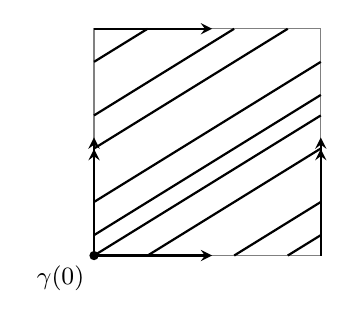
\begin{tikzpicture}[scale=1.2,>=stealth]
        \draw[gray] (0,0) rectangle (2.4,2.4);
        \draw[thick,->] (0,0)--(1.25,0); \draw[thick,->] (0,2.4)--(1.25,2.4);
        \draw[thick,->>] (0,0)--(0,1.25); \draw[thick,->>] (2.4,0)--(2.4,1.25);
        \draw[thick] (0.000,0.000)--(2.400,1.483);
        \draw[thick] (0.000,1.483)--(1.483,2.400);
        \draw[thick] (1.483,0.000)--(2.400,0.567);
        \draw[thick] (0.000,0.567)--(2.400,2.050);
        \draw[thick] (0.000,2.050)--(0.567,2.400);
        \draw[thick] (0.567,0.000)--(2.400,1.133);
        \draw[thick] (0.000,1.133)--(2.050,2.400);
        \draw[thick] (2.050,0.000)--(2.400,0.216);
        \draw[thick] (0.000,0.216)--(2.400,1.700);
        \fill (0,0) circle (1.4pt);
        \node[below left] at (0,0) {\small $\gamma(0)$};
    \end{tikzpicture}
    \caption{The first few windings of a line of irrational slope on the torus, drawn as a square with opposite sides glued (single and double arrows). The line never closes up, and it comes back arbitrarily close to every point, including $\gamma(0)$.}
    \label{fig irrational winding}
\end{figure}

\begin{example}\label{example immersions embeddings}\index{Cusp}
    \begin{enumerate}
        \item The map $\bbS^1\to\bbR^2$, $\rme^{\rmi t}\mapsto(\sin2t,\sin t)$, is an immersion whose image is the figure eight. It is not injective, since $t=0$ and $t=\pi$ have the same image. Its restriction to $t\in(-\pi,\pi)$ is the injective immersion $\beta$, which is not an embedding (Example~\ref{example not embeddings}); note also that its image is compact, while $(-\pi,\pi)$ is not.
        \item The line of irrational slope $\gamma(t)=(\rme^{2\pi\rmi t},\rme^{2\pi\rmi\alpha t})$ on $\bbT^2$, $\alpha\notin\bbQ$, is a smooth injective immersion, but not an embedding (Example~\ref{example not embeddings}). It is also a homomorphism of groups $\bbR\to\bbT^2$; we will return to it in Example~\ref{example dense subgroup of torus}.
        \item The map $x\mapsto(x^3,0)$ is a topological embedding $\bbR\hookrightarrow\bbR^2$ and smooth, but it is not a smooth embedding, since its differential vanishes at $0$. Its image is the $x$-axis, which is perfectly smooth, but the smooth structure that the map induces on it, given by the chart $(y,0)\mapsto y^{1/3}$, is not the standard one (cf.\ Example~\ref{example smooth atlases}).
        \item The condition on the differential is what prevents the image of a smooth embedding from having corners or cusps. The curve $t\mapsto(t^2,t^3)$ is a smooth topological embedding whose image has a cusp at the origin, and the curve $t\mapsto\big(h(t)-h(-t),\,h(t)+h(-t)\big)$, with $h$ as in Lemma~\ref{lem smooth bumps}, is a smooth topological embedding whose image near the origin is the graph of $\lvert x\rvert$ (Figure~\ref{fig cusp}). In both cases, the velocity vanishes at $t=0$.
    \end{enumerate}
\end{example}

\begin{figure}[tp]
    \centering
    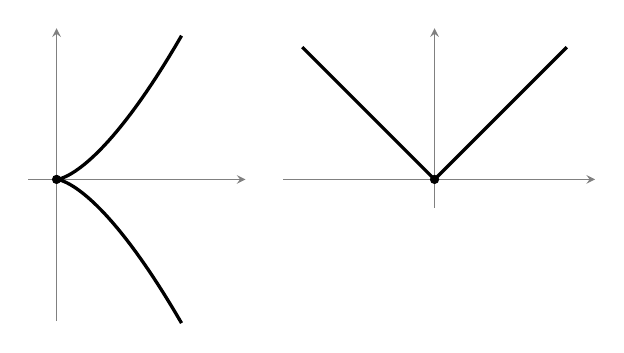
\begin{tikzpicture}[scale=1.2,>=stealth]
        \draw[gray,->] (-0.3,0)--(2.0,0);
        \draw[gray,->] (0,-1.5)--(0,1.6);
        \draw[very thick,domain=-1.15:1.15,samples=80] plot ({\x*\x},{\x*\x*\x});
        \fill (0,0) circle (1.4pt);
        \begin{scope}[xshift=4cm]
            \draw[gray,->] (-1.6,0)--(1.7,0);
            \draw[gray,->] (0,-0.3)--(0,1.6);
            \draw[very thick] (-1.4,1.4)--(0,0)--(1.4,1.4);
            \fill (0,0) circle (1.4pt);
        \end{scope}
    \end{tikzpicture}
    \caption{Images of smooth injective curves whose velocity vanishes at one point: the cusp $t\mapsto(t^2,t^3)$ (left), and a curve tracing the graph of $\lvert x\rvert$ (right). Neither is an immersion.}
    \label{fig cusp}
\end{figure}

\begin{prop}[{{\cite[Prop.~4.22]{Lee}}}]\label{prop injective immersion embedding}
    An injective immersion $f:M\to N$ is a smooth embedding if any of the following holds:
    \begin{enumerate}
        \item $f$ is open or closed;
        \item $f$ is proper;
        \item $M$ is compact;
        \item $\partial M=\varnothing$ and $\dim M=\dim N$.
    \end{enumerate}
\end{prop}
\begin{proof}
    (1) If $f$ is open (or closed), then the image of every open (closed) subset of $M$ is open (closed) in $N$, hence in $f(M)$, so $f^{-1}:f(M)\to M$ is continuous. (2) Proper maps between manifolds are closed (Proposition~\ref{prop proper closed}). (3) Maps from compact spaces to Hausdorff spaces are closed (Proposition~\ref{prop compact to Hausdorff}). (4) In this case, $f$ is a local diffeomorphism by the inverse mapping theorem, hence open.
\end{proof}

\begin{thm}[Local embedding theorem {{\cite[Thm.~4.25]{Lee}}}]\label{thm.local embedding}
    A smooth map $f:M\to N$ is an immersion iff every point of $M$ has a neighborhood $U$ such that $\restr{f}{U}$ is a smooth embedding.
\end{thm}
\begin{proof}
    If $f$ is an immersion and $M$ and $N$ have no boundary, then by the rank theorem, near every point $f$ is the inclusion $\bbR^m\hookrightarrow\bbR^n$ of a coordinate plane in suitable charts, which is an embedding. (At boundary points, see the cited reference.) The converse holds by definition.
\end{proof}


\section{Submanifolds}\label{sec submanifolds}
Immersions and embeddings give rise to the notions of immersed and embedded submanifolds.

\begin{defn}[Submanifolds]\index{Submanifold!Immersed}\index{Submanifold!Embedded}\index{Submanifold!Weakly embedded}\index{Submanifold!Initial}\index{Submanifold!Properly embedded}\index{Submanifold}
    Let $S$ and $M$ be smooth manifolds and $i:S\to M$ a smooth map. The pair $(S,i)$ is called
    \begin{enumerate}
        \item an \emph{immersed submanifold} if $i$ is an injective immersion. We write $S<M$;\index{$<$}
        \item a \emph{weakly embedded submanifold}, or an \emph{initial submanifold}, if it is immersed and every smooth map $f:N\to M$ with $f(N)\subset i(S)$ is smooth as a map $f:N\to S$. We write $S\embweak M$;
        \item an \emph{embedded submanifold} if $i$ is a smooth embedding. We write $S\emb M$;\index{$\emb$}
        \item a \emph{properly embedded submanifold} if $i$ is a proper smooth embedding. We write $S\embprop M$.\index{$\embprop$}
    \end{enumerate}
    The \emph{codimension}\index{Codimension} of the submanifold is $\codim S=\dim M-\dim S$.
\end{defn}
We usually identify $S$ with the subset $i(S)\subset M$, with $i$ the inclusion. Often we start with a subset $S\subset M$ with the subspace topology; then the only question is whether it has a smooth structure that turns the inclusion into an immersion. Images of non-injective immersions, such as the figure eight in Example~\ref{example immersions embeddings}, are sometimes also called immersed submanifolds, but we avoid this, since such subsets are not manifolds themselves.

\begin{example}\label{example submanifolds}
    \begin{enumerate}
        \item Any open subset is an embedded submanifold of codimension zero.
        \item If $F:N\to M$ is a smooth embedding, then $F(N)$, with the smooth structure transported from $N$, is an embedded submanifold of $M$. Thus, embedded submanifolds are exactly the images of smooth embeddings.
        \item Compact embedded submanifolds are properly embedded, because they are closed (Proposition~\ref{prop properly embedded closed}).
        \item If $f\in C^\infty(N,M)$, then its graph $\graph(f)\subset N\times M$ is a properly embedded submanifold: it is the image of the embedding $x\mapsto(x,f(x))$, whose inverse is the restriction of the projection to $N$.
        \item The inverse of the stereographic projection is an embedding $\bbR^n\hookrightarrow\bbS^n$ onto $\bbS^n\setminus\{N\}$. It is not proper, since its image is not closed.
        \item The figure eight curve $\beta$ of Figure~\ref{fig figure eight} is an immersed submanifold that is not weakly embedded. Indeed, the curve $c(s)=(\sin2s,-\sin s)$, $s\in(-\epsilon,\epsilon)$, is smooth and takes values in the figure eight. But it passes through the origin along the two ``end'' branches of the figure eight: $c(s)=\beta(\pi+s)$ for $s<0$ and $c(s)=\beta(-\pi+s)$ for $s>0$, while $c(0)=\beta(0)$. As a map into $(-\pi,\pi)$, it jumps from $\pi$ to $0$ to $-\pi$.
        \item \emph{A smooth topologist's sine curve.} Let $S\subset\bbR^2$ be the union of the vertical segment $\{0\}\times(-2,1)$, the graph $\Gamma$ of $\sin\frac1x$, $0<x\leq1$, and a smooth arc joining $(0,-2)$ to $(1,\sin1)$ and avoiding everything else (Figure~\ref{fig smooth sine curve}). It is the image of an injective immersion of $\bbR$ that runs down the segment, along the arc, and then along $\Gamma$ towards the $y$-axis. As in Example~\ref{example sine curve}, the graph accumulates on the segment, so $S$ is not embedded: with the subspace topology, $S$ is not even locally connected at the points $(0,y_0)$ with $-1\leq y_0<1$. But $S$ is weakly embedded. Near all points outside the segment $\{0\}\times[-1,1]$, the two topologies agree. So let $f:N\to\bbR^2$ be smooth with $f(N)\subset S$ and $f(p)=(0,y_0)$ with $-1\leq y_0<1$. For a small ball $B$ of radius less than $1$ around $(0,y_0)$, the set $S\cap B$ consists of a piece of the segment and of arcs of $\Gamma$, and each of these arcs is both open and closed in $S\cap B$. If $W$ is a connected neighborhood of $p$ with $f(W)\subset B$, then the connected set $f(W)$ contains a point of the segment, so it cannot meet any of the arcs. Thus $f$ maps $W$ into the segment, where the topology of $S$ is the subspace topology, so $f$ is continuous into $S$ near $p$, hence smooth by Theorem~\ref{thm restrictions to submfds}. Compare this with the figure eight: there, a curve in $\bbR^2$ \emph{can} pass from one branch to another.
        \item The line of irrational slope on the torus (Figure~\ref{fig irrational winding}) is weakly embedded, but not embedded. It is a Lie subgroup of $\bbT^2$, and all Lie subgroups are weakly embedded (Theorem~\ref{thm 19.25 Lee}).
    \end{enumerate}
\end{example}

\begin{figure}[tp]
    \centering
    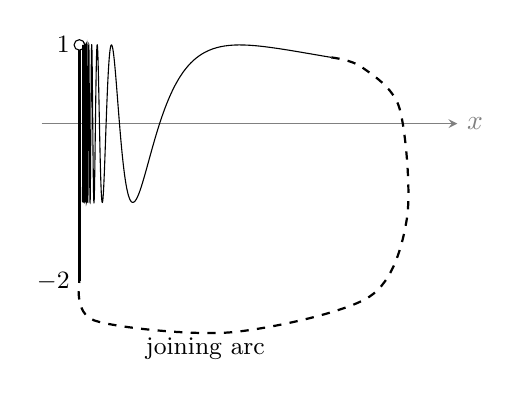
\begin{tikzpicture}[xscale=3.2,yscale=1.0,>=stealth]
        \draw[->,gray] (-0.15,0)--(1.5,0) node[right]{$x$};
        \draw[very thick] (0,-2)--(0,1);
        \draw[fill=white] (0,1) circle (0.6pt and 1.9pt);
        \draw[domain=1:80,samples=1500,variable=\u] plot ({1/\u},{sin(\u r)});
        \draw[thick,dashed] plot[smooth] coordinates {(1,0.8415) (1.12,0.72) (1.27,0.2) (1.3,-1.2) (1.15,-2.2) (0.6,-2.65) (0.06,-2.5) (0,-2)};
        \node[left] at (0,1) {\small $1$};
        \node[left] at (0,-2) {\small $-2$};
        \node[below] at (0.5,-2.6) {\small joining arc};
    \end{tikzpicture}
    \caption{A smooth topologist's sine curve: the segment $\{0\}\times(-2,1)$ (thick), the graph of $\sin\frac1x$ (thin), and an arc joining them (dashed) form the image of an injective immersion of $\bbR$. It is weakly embedded but not embedded.}
    \label{fig smooth sine curve}
\end{figure}

\begin{prop}[{{\cite[Prop.~5.18]{Lee}}}]\label{prop 5.18 Lee}
    If $F:N\to M$ is an injective immersion, then $F(N)$ has a unique topology and smooth structure such that it is an immersed submanifold of $M$ and $F:N\to F(N)$ is a diffeomorphism.
\end{prop}
\begin{proof}
    The topology and smooth structure are transported by $F$: a set $U\subset F(N)$ is open iff $F^{-1}(U)$ is open, and the charts are $(F(U),\varphi\circ F^{-1})$ for the charts $(U,\varphi)$ of $N$. They make $F:N\to F(N)$ a diffeomorphism, and are the only ones with this property. The inclusion $F(N)\hookrightarrow M$ is the composite of the diffeomorphism $F^{-1}:F(N)\to N$ and the immersion $F$, so it is an immersion.
\end{proof}

Embedded submanifolds have a simple local description: they look like coordinate planes in suitable charts (Figure~\ref{fig slice chart}).

\begin{prop}[Slice charts {{\cite[Thm.~5.8]{Lee}}}]\label{prop slice charts}\index{Slice chart}
    A subset $S$ of a manifold $M^m$ is an embedded $k$-dimensional submanifold iff every point $p\in S$ is in the domain of a \emph{slice chart} $(U,\varphi)$ of $M$, i.e., a chart such that
    \[\varphi(S\cap U)=\varphi(U)\cap\big(\bbR^k\times\{0\}\big)=\{\bf{x}\in\varphi(U)\mid x^{k+1}=\ldots=x^m=0\}.\]
    In this case, the restrictions of the slice charts to $S$ form a smooth atlas on $S$, and the resulting smooth structure is the unique one for which $S\emb M$.
\end{prop}
\begin{proof}
    If $S\emb M$, then by the rank theorem, near $p$ the inclusion has the local representative $\bf{x}\mapsto(\bf{x},0)$ in suitable charts $\psi$ of $S$ and $\varphi$ of $M$, defined on a small neighborhood $V$ of $p$ in $S$. Since $S$ carries the subspace topology, $V=S\cap W$ for an open set $W\subset M$, and shrinking the domain of $\varphi$ to the part of it inside $W$ whose image lies in $\psi(V)\times\bbR^{m-k}$ gives a slice chart. Conversely, the transition maps between restricted slice charts are restrictions of the smooth transition maps of $M$ to coordinate planes, hence smooth. In these charts, the inclusion is $\bf{x}\mapsto(\bf{x},0)$, an immersion, and $S$ carries the subspace topology by construction. Uniqueness is Theorem~\ref{thm 5.31 Lee} below.
\end{proof}

\begin{figure}[tp]
    \centering
    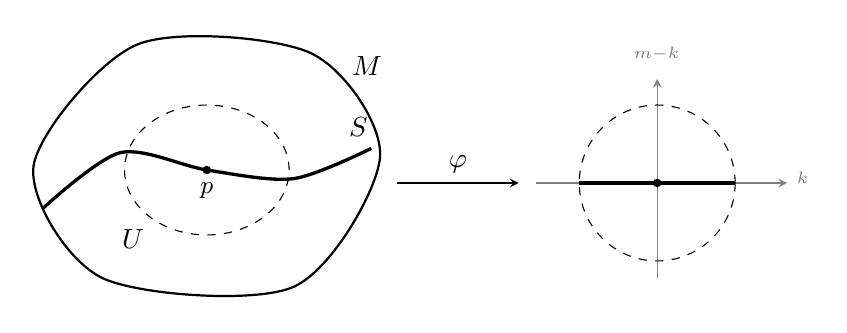
\begin{tikzpicture}[scale=1.1,>=stealth]
        \draw[thick] plot[smooth cycle] coordinates {(-2.6,0.2) (-1.4,1.6) (0.6,1.5) (1.4,0.3) (0.4,-1.2) (-1.8,-1.1)};
        \node at (1.25,1.35) {$M$};
        \draw[dashed] (-0.6,0.15) ellipse (0.95 and 0.75);
        \node at (-1.45,-0.65) {$U$};
        \draw[very thick] plot[smooth] coordinates {(-2.5,-0.3) (-1.6,0.35) (-0.6,0.15) (0.4,0.05) (1.3,0.4)};
        \node[above] at (1.15,0.42) {$S$};
        \fill (-0.6,0.15) circle (1.4pt);
        \node[below] at (-0.6,0.12) {\small $p$};
        \draw[->] (1.6,0.0)--(3.0,0.0) node[midway,above] {$\varphi$};
        \begin{scope}[xshift=4.6cm]
            \draw[gray,->] (-1.4,0)--(1.5,0) node[right] {\small $\bbR^k$};
            \draw[gray,->] (0,-1.1)--(0,1.2) node[above] {\small $\bbR^{m-k}$};
            \draw[dashed] (0,0) circle (0.9);
            \draw[very thick] (-0.9,0)--(0.9,0);
            \fill (0,0) circle (1.4pt);
        \end{scope}
    \end{tikzpicture}
    \caption{A slice chart $(U,\varphi)$ (dashed) maps $S\cap U$ onto a piece of the coordinate plane $\bbR^k\times\{0\}$.}
    \label{fig slice chart}
\end{figure}

\begin{cor}
    The boundary $\partial M$ of a manifold with boundary is an embedded submanifold of codimension one: in boundary charts, it is the coordinate plane $x^n=0$.
\end{cor}

\begin{prop}\label{prop properly embedded closed}
    An embedded submanifold $S\subset M$ is properly embedded iff it is a closed subset of $M$.
\end{prop}
\begin{proof}
    If $S$ is closed and $K\subset M$ is compact, then $S\cap K$ is a closed subset of $K$, hence compact. Conversely, a proper map into a manifold has a closed image (Proposition~\ref{prop proper closed}).
\end{proof}

The most important source of embedded submanifolds is the following theorem. It is the global version of the implicit mapping theorem: a system of equations whose derivatives are linearly independent defines a manifold.

\begin{thm}[Level set theorem]\index{Theorem!Level set}\label{thm level set submanifold}
    Let $M$ and $N$ be manifolds without boundary. If $f\in C^\infty(M,N)$ has constant rank $r$, then each level set $f^{-1}(q)$, $q\in N$, is a properly embedded submanifold of codimension $r$, and
    \[\T_mf^{-1}(q)=\ker f_{\ast m}\quad\text{for all }m\in f^{-1}(q).\]
\end{thm}
\begin{proof}
    By the rank theorem, near any point of $f^{-1}(q)$ there are charts in which $f$ takes the normal form of Theorem~\ref{Rank thm} and $q$ is the origin. In such a chart, $f^{-1}(q)=\{x^1=\ldots=x^r=0\}$ is a coordinate plane of dimension $m-r$, so, after permuting the coordinates, these charts are slice charts. The level set is closed as the preimage of a point, hence properly embedded. Finally, $f$ is constant on $f^{-1}(q)$, so $f_{\ast m}$ vanishes on its tangent space, and both $\T_mf^{-1}(q)$ and $\ker f_{\ast m}$ have dimension $m-r$.
\end{proof}

\begin{cor}
    Each level set of a smooth submersion $f:M\to N$ is a properly embedded submanifold of codimension $\dim N$.
\end{cor}

\begin{cor}[Regular level set theorem]\label{thm regular level set}\index{Theorem!Regular level set}
    Every level set $f^{-1}(q)$ of a regular value $q$ of a smooth map $f:M\to N$ is a properly embedded submanifold of codimension $\dim N$.
\end{cor}
\begin{proof}
    The set of regular points is open (Proposition~\ref{domain of maximal rank}) and contains $f^{-1}(q)$. Apply the previous corollary to the restriction of $f$ to this open set.
\end{proof}

Critical level sets can be singular, as in Figure~\ref{fig level sets}, or even arbitrary closed sets (Theorem~\ref{thm closed sets are zero sets}). By Sard's theorem, however, almost all level sets are regular.

\begin{figure}[tp]
    \centering
    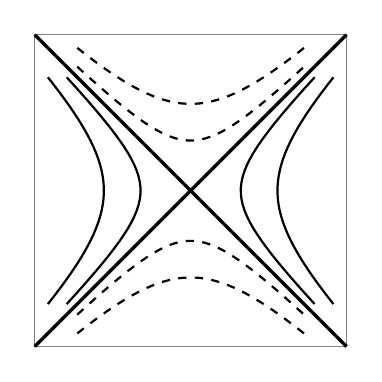
\begin{tikzpicture}[scale=0.9,>=stealth]
        \clip (-2.3,-2.3) rectangle (2.3,2.3);
        \draw[gray] (-2.2,-2.2) rectangle (2.2,2.2);
        \draw[very thick] (-2.2,-2.2)--(2.2,2.2) (-2.2,2.2)--(2.2,-2.2);
        \foreach \c in {0.5,1.5} {
            \draw[thick,domain=-1.6:1.6,samples=40] plot ({sqrt(\c+\x*\x)},\x);
            \draw[thick,domain=-1.6:1.6,samples=40] plot ({-sqrt(\c+\x*\x)},\x);
            \draw[thick,dashed,domain=-1.6:1.6,samples=40] plot (\x,{sqrt(\c+\x*\x)});
            \draw[thick,dashed,domain=-1.6:1.6,samples=40] plot (\x,{-sqrt(\c+\x*\x)});
        }
    \end{tikzpicture}
    \caption{Level sets of $f(x,y)=x^2-y^2$. The level sets of the regular values $c>0$ (solid) and $c<0$ (dashed) are hyperbolas, which are $1$-manifolds. The level set of the only critical value $0$ is a cross (thick), which is not.}
    \label{fig level sets}
\end{figure}

\begin{example}\label{example level sets}
    \begin{enumerate}
        \item The sphere $\bbS^n=f^{-1}(1)$ for $f(\bf{x})=\lvert\bf{x}\rvert^2$, whose differential $f_{\ast\bf{x}}(\bf{v})=2\bf{x}\cdot\bf{v}$ is surjective for $\bf{x}\neq0$. The level set theorem recovers $\T_{\bf{x}}\bbS^n=\ker f_{\ast\bf{x}}=\bf{x}^\perp$, and, by Theorem~\ref{thm 5.31 Lee} below, it shows that the smooth structure given by the hemisphere or stereographic charts (Example~\ref{example smooth atlases}) is the unique one making $\bbS^n$ an embedded submanifold of $\bbR^{n+1}$.
        \item The torus of revolution $\big(\sqrt{x^2+y^2}-R\big)^2+z^2=r^2$, $0<r<R$, is a regular level set in $\bbR^3$. The height function of Example~\ref{example critical values} is the restriction of $x$ to it (the torus ``stands upright'' along the $x$-axis).
        \item The double cone $x^2+y^2-z^2=0$ of Figure~\ref{fig double cone} is the level set of the critical value $0$; all other level sets are hyperboloids. Its upper half $C_+$, which is a smooth manifold by Example~\ref{example smooth atlases}, is not an embedded submanifold of $\bbR^3$. Otherwise, by Theorem~\ref{thm restrictions to submfds}, the rays $t\mapsto t(\cos\theta,\sin\theta,1)$, $t\in[0,\epsilon)$, would be smooth curves in $C_+$, and their velocities would lie in the $2$-dimensional tangent space at the apex. But these velocities span $\bbR^3$.
    \end{enumerate}
\end{example}

\begin{example}[Classical groups as manifolds]\label{example classical groups manifolds}\index{Group!classical}\index{Orthogonal group}\index{Special linear group}\index{Unitary group}
    \begin{enumerate}
        \item By Example~\ref{example rank}, $\det:\GL_n(\bbR)\to\bbR$ is a submersion, so $\SL_n(\bbR)=\det^{-1}(1)$ is a properly embedded submanifold of dimension $n^2-1$. Its tangent space at the identity is $\ker\det\nolimits_{\ast\rmI_n}=\{H\mid\tr H=0\}$.
        \item By the same example, $F(A)=A^\top A$ is a submersion $\GL_n(\bbR)\to\Sym_n$, so $\Or_n=F^{-1}(\rmI_n)$ is a properly embedded submanifold of $\GL_n(\bbR)$, of dimension $n^2-\frac{n(n+1)}2=\frac{n(n-1)}2$. Its tangent space at the identity consists of the skew-symmetric matrices, $\T_{\rmI_n}\Or_n=\ker F_{\ast\rmI_n}=\{H\mid H^\top+H=0\}$. Since $\Or_n$ is closed in $\Mat_n(\bbR)$, it is also a properly embedded submanifold of $\Mat_n(\bbR)$. For the unitary group $\U_n$, see Exercise~\ref{xca boundary of level set}.
    \end{enumerate}
    For $n=3$, we find again that the configuration space $\SO_3$ of a rigid body, a component of $\Or_3$, is a $3$-manifold. The multiplication and inversion maps of these groups are smooth, which makes them Lie groups (\S\ref{sec: classical groups}).
\end{example}

\begin{xca}\label{xca boundary of level set}
    \begin{enumerate}
        \item Let $M$ be a manifold with boundary, and let $q\in N$ be a regular value of both $f\in C^\infty(M,N)$ and $\restr{f}{\partial M}$. Show that $f^{-1}(q)$ is a manifold with boundary $f^{-1}(q)\cap\partial M$. \emph{Hint:} at a boundary point, reduce to a level set of a submersion from $\wb\bbR^m_+$, and use the coordinate $x^m$ as a function on that level set.
        \item Show that the unitary group $\U_n$ is a submanifold of $\GL_n(\bbC)$ of real dimension $n^2$, and compute $\T_{\rmI_n}\U_n$.
    \end{enumerate}
\end{xca}

Sard's theorem and the regular level set theorem combine into a strikingly simple proof of a classical result, due to M.~Hirsch.

\begin{thm}\label{thm no smooth retraction}\index{Theorem!No smooth retraction}
    There is no smooth retraction $r:\wb{B^n}\to\bbS^{n-1}$, i.e., no smooth map with $r(\bf{x})=\bf{x}$ for all $\bf{x}\in\bbS^{n-1}$.
\end{thm}
\begin{proof}
    By Sard's theorem, the restriction of $r$ to the open ball has a regular value $\bf{q}\in\bbS^{n-1}$. All values of $\restr{r}{\bbS^{n-1}}=\id$ are regular. By Exercise~\ref{xca boundary of level set}, $r^{-1}(\bf{q})$ is a compact $1$-manifold with boundary $r^{-1}(\bf{q})\cap\bbS^{n-1}=\{\bf{q}\}$. But a compact $1$-manifold has an even number of boundary points (Remark~\ref{rem classification of 1-manifolds}).
\end{proof}

\begin{cor}\label{cor Brouwer smooth}\index{Theorem!Brouwer's fixed point}
    Brouwer's fixed point theorem (Theorem~\ref{thm Brouwer's fixed point}) holds for all $n\geq1$, and the sphere $\bbS^{n-1}$ is not contractible.
\end{cor}
\begin{proof}
    If a smooth $f:\wb{B^n}\to\wb{B^n}$ has no fixed point, then the ray construction of Figure~\ref{fig Brouwer} gives a retraction $h(\bf{x})=\bf{x}+t(\bf{x})(\bf{x}-f(\bf{x}))$, where $t(\bf{x})\geq0$ is the nonnegative root of the quadratic equation $\lvert h(\bf{x})\rvert^2=1$. Its discriminant is positive everywhere: it could only vanish at points of the boundary sphere where $\bf{x}\cdot(\bf{x}-f(\bf{x}))=0$, i.e., $\bf{x}\cdot f(\bf{x})=1$, which forces $f(\bf{x})=\bf{x}$. So $t$ and $h$ are smooth, contradicting the theorem.

    If a continuous $f$ has no fixed point, then $\lvert f(\bf{x})-\bf{x}\rvert\geq\epsilon>0$ on the compact ball. We may take $\epsilon<2$. By the Weierstrass approximation theorem, there is a polynomial map $p$ with $\lvert p-f\rvert<\epsilon/4$ on the ball, and then $g=p/(1+\epsilon/4)$ maps the ball into itself, is smooth, and satisfies $\lvert g-f\rvert<\epsilon/2$. So $g$ has no fixed point either, a contradiction. Finally, a contraction of $\bbS^{n-1}$ would give a map of the ball without fixed points (Remark~\ref{rem Brouwer equivalent}).
\end{proof}
This gives an analytic proof of Theorem~\ref{thm spheres not contractible}, which was used in \S\ref{sec.homotopy}; another proof, using homology, is given in Corollary~\ref{cor Brouwer homology}.

\begin{prop}[Local defining functions]\label{prop local defining functions}\index{Local defining function}
    If $S\emb M$ is an embedded submanifold of codimension $k$, then every point of $S$ has a neighborhood $U$ in $M$ and a submersion $\varPhi:U\to\bbR^k$ with $S\cap U=\varPhi^{-1}(0)$.
\end{prop}
\begin{proof}
    In a slice chart, take $\varPhi=(x^{m-k+1},\ldots,x^m)$.
\end{proof}
So, locally, every embedded submanifold is a regular level set. Globally this fails, as the core circle $C$ of the M\"obius band (Figure~\ref{fig square gluings}) shows. If $C=f^{-1}(0)$ for a function $f$ with $f_{\ast}\neq0$ on $C$, then $f$ takes both signs near every point of $C$, so the complement of $C$ would be the disjoint union of the nonempty open sets $\{f>0\}$ and $\{f<0\}$. But the complement of $C$ in the (open) M\"obius band is connected.

For an immersed submanifold $S<M$, sufficiently small neighborhoods of points \emph{in $S$} are embedded by Theorem~\ref{thm.local embedding}. However, $S\cap V$ need not be embedded for any neighborhood $V$ of a point in $M$: for the line of irrational slope, $S\cap V$ consists of infinitely many segments accumulating on each other.

\begin{thm}[Extension of functions]\label{thm extension from submanifolds}\index{Extension of functions from submanifolds}
    \begin{enumerate}
        \item If $S\emb M$, then every $f\in C^\infty(S)$ extends to a smooth function on some open neighborhood of $S$ in $M$.
        \item If $S\embprop M$, then every $f\in C^\infty(S)$ extends to a smooth function on $M$.
    \end{enumerate}
\end{thm}
\begin{proof}
    (1) In a slice chart, $f$ extends to the slice chart domain by making it independent of the coordinates $x^{k+1},\ldots,x^m$. The union $U$ of the domains of these slice charts is an open neighborhood of $S$, and $S$ is closed in $U$, so the extension lemma (Theorem~\ref{extension lemma}) applied in $U$ glues these local extensions. (2) $S$ is closed in $M$, so we can apply the extension lemma in $M$ directly.
\end{proof}

\begin{xca}
    Show that the two conditions of the last theorem characterize embedded and properly embedded submanifolds among immersed ones, respectively.
\end{xca}

\begin{thm}[Restrictions to submanifolds {{\cite[Thms.~5.27-30]{Lee}}}]\label{thm 5.27 Lee}\label{thm restrictions to submfds}
    Let $f\in C^\infty(M,N)$.
    \begin{enumerate}
        \item If $S<M$, then the restriction $\restr{f}{S}:S\to N$ is smooth.
        \item If $K<N$, $f(M)\subset K$, and $f$ is continuous as a map $M\to K$, then $f$ is smooth as a map $M\to K$.
        \item If $K\emb N$ and $f(M)\subset K$, then $f$ is smooth as a map $M\to K$.
    \end{enumerate}
\end{thm}
\begin{proof}
    (1) $\restr{f}{S}=f\circ i$ is a composite of smooth maps. For (2) and (3), see the cited reference: (3) follows from (2), since $f$ is automatically continuous into $K$ with its subspace topology, and (2) follows from the local embedding theorem.
\end{proof}

Thus, to restrict a smooth map in the codomain to an immersed submanifold $K$, we need it to be continuous as a map into $K$. Weakly embedded submanifolds are exactly the immersed submanifolds for which this condition is automatic. Their definition is the smooth analog of the universal property of the initial topology (Proposition~\ref{prop initial final universal}).

\begin{rem}
    The terminology around submanifolds varies, and only the concept of embedded submanifolds is consistent across different authors. Our use of the term ``immersed submanifold'' (the image of an injective immersion) agrees with \cite{Lee}. Weakly embedded submanifolds are called this way in \cite{Lee} and initial in \cite{RS1}. We have the strict inclusions
    \[\text{proper embeddings}\subset\text{embeddings}\subset\text{weak embeddings}\subset\text{injective immersions}.\]
\end{rem}

\begin{thm}[{{\cite[Thm.~5.31]{Lee}}}]\label{thm 5.31 Lee}
    If $S\emb M$ is embedded, then the subspace topology on $S$ and the smooth structure given by slice charts are the only topology and smooth structure with respect to which $S$ is an embedded or even immersed submanifold.
\end{thm}

\begin{thm}[{{\cite[Thm.~5.32]{Lee}}}]\label{thm 5.32 Lee}
    If $S<M$ is immersed, then for a given topology on $S$ there is only one smooth structure making $S$ into an immersed submanifold.
\end{thm}

It is certainly possible for a given subset of $M$ to have more than one topology making it an immersed submanifold: the figure eight can be parametrized as in Figure~\ref{fig figure eight}, or with the origin attached to the other two branches. For weakly embedded submanifolds this cannot happen.

\begin{thm}[{{\cite[Thm.~5.33]{Lee}}}]\label{thm 5.33 Lee}
    If $S\subset M$ is a weakly embedded submanifold, then $S$ has only one topology and smooth structure with respect to which it is an immersed submanifold.
\end{thm}


\section{Submersions}\label{sec: submersions}

Recall from \S\ref{sec: classes of morphisms} that a split epimorphism is a morphism with a right inverse, or section. In $\mathsf{Man}^\infty$, as in the category of Hausdorff spaces, the epimorphisms are exactly the maps with dense images, while split epimorphisms have to be surjective. (A map with a dense image is an epimorphism by Proposition~\ref{prop dense determines maps}; if the image is not dense, a bump function supported away from it shows that the map is not an epimorphism in $\mathsf{Man}^\infty$.) Submersions are the maps that are split epimorphisms locally.

\begin{defn}[Local section]\index{Section}
    A \emph{local section}\index{Local section} of a continuous (or smooth) map $\pi:M\to N$ is a continuous (respectively, smooth) map $\sigma:V\to M$ defined on an open set $V\subset N$ such that $\pi\circ\sigma=\id_V$.
\end{defn}

\begin{thm}[Local section theorem {{\cite[Thm.~4.26]{Lee}}}]\index{Theorem!Local Section}\label{thm: local section}
    A smooth map $\pi:M\to N$ between manifolds without boundary is a submersion iff every point $m\in M$ lies in the image of a smooth local section of $\pi$ (Figure~\ref{fig local section}).
\end{thm}
\begin{proof}
    If $\pi$ is a submersion, then by the rank theorem, in suitable charts centered at $m$ and $\pi(m)$ it is the projection onto the first $n$ coordinates, and $\bf{y}\mapsto(\bf{y},0)$ is a local section through $m$. Conversely, if $\sigma$ is a local section with $\sigma(q)=m$, then differentiating $\pi\circ\sigma=\id$ gives $\pi_{\ast m}\circ\sigma_{\ast q}=\id_{\T_qN}$, so $\pi_{\ast m}$ is surjective.
\end{proof}

\begin{figure}[tp]
    \centering
    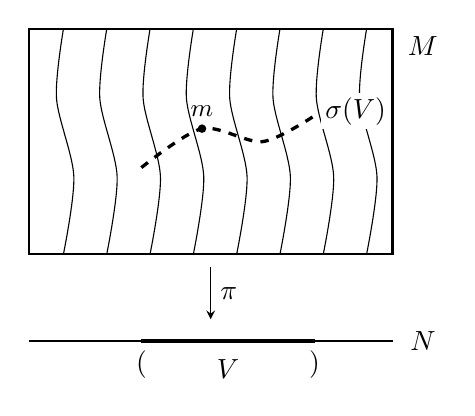
\begin{tikzpicture}[scale=1.1,>=stealth]
        \draw[thick] (0,1)--(4.2,1)--(4.2,3.6)--(0,3.6)--cycle;
        \node at (4.55,3.4) {$M$};
        \foreach \x in {0.4,0.9,...,3.9} \draw plot[smooth] coordinates {(\x,1) ({\x+0.12},1.9) ({\x-0.08},2.8) (\x,3.6)};
        \draw[very thick,dashed] plot[smooth] coordinates {(1.3,2.0) (2.0,2.45) (2.7,2.3) (3.3,2.6)};
        \fill (2.0,2.45) circle (1.4pt);
        \node[above] at (2.0,2.48) {\small $m$};
        \node[right,fill=white,inner sep=1.5pt] at (3.37,2.65) {$\sigma(V)$};
        \draw[->] (2.1,0.85)--(2.1,0.25) node[midway,right] {$\pi$};
        \draw[thick] (0,0)--(4.2,0);
        \node at (4.55,0) {$N$};
        \draw[very thick] (1.3,0)--(3.3,0);
        \node[below] at (1.3,0) {$($}; \node[below] at (3.3,0) {$)$};
        \node[below] at (2.3,-0.1) {$V$};
    \end{tikzpicture}
    \caption{The fibers of a submersion $\pi:M\to N$ (thin curves) and a local section $\sigma$ through the point $m$ (dashed), defined over an open set $V\subset N$ (thick).}
    \label{fig local section}
\end{figure}

This motivates a topological version of submersions.

\begin{defn}[Topological submersion]\index{Submersion!topological}
    A continuous map $f:X\to Y$ is a \emph{topological submersion} if every $x\in X$ lies in the image of a continuous local section of $f$.
\end{defn}
A narrower topological notion is obtained by reading the rank theorem: around every point $x\in X$ there should be neighborhoods $U$ of $x$ and $V$ of $f(x)$ and a homeomorphism $\phi:U\to V\times Z$, for some space $Z$, such that $\restr{f}{U}=\pr_1\circ\phi$. In simple terms, such a map locally looks like a Cartesian projection. In the topological category, these maps form a proper subclass of the topological submersions, while in the smooth category the two notions coincide by the theorem above.

Next, we look for the smooth analog of a quotient map. Recall that a topological quotient map is a continuous surjection onto a space with the final topology, i.e., $V$ is open iff $f^{-1}(V)$ is open. A continuous surjection that is open is a quotient map, but not every quotient map is open: for example, the map $\wb{B^n}\to\wb{B^n}/\bbS^{n-1}\cong\bbS^n$ collapsing the boundary sphere is not (Example~\ref{example collapsing}). In fact, a continuous surjection $q$ is a quotient map iff it sends open sets that are unions of fibers of $q$ to open sets. These subtleties disappear in the smooth case.

\begin{prop}\label{thm submersions are open quotient maps}
    Every smooth submersion $\pi:M\to N$ is an open map. In particular, every surjective submersion is a topological quotient map.
\end{prop}
\begin{proof}
    Let $W\subset M$ be open and $m\in W$. Take a local section $\sigma$ through $m$, $\sigma(q)=m$. Then $\sigma^{-1}(W)$ is an open neighborhood of $q=\pi(m)$, and it lies in $\pi(W)$, since $y=\pi(\sigma(y))$. So $\pi(W)$ is a neighborhood of each of its points.
\end{proof}

\begin{defn}[Smooth quotient map]\index{Quotient map!in smooth category}
    A \emph{smooth quotient map} is a surjective submersion.
\end{defn}
Since a submersion $f:M\to N$ is open, its image $f(M)$ is an open submanifold, and $f:M\to f(M)$ is a smooth quotient map. With this remark, \emph{smooth submersions and smooth quotient maps are essentially the same thing}. Smooth quotient maps have the same universal property as topological ones (Proposition~\ref{prop initial final universal}).

\begin{thm}[Characteristic property of surjective submersions]\label{thm characteristic property submersions}\index{Universal property!of surjective submersions}
    Let $\pi:M\to N$ be a surjective submersion and $F:N\to P$ any map to a manifold $P$. Then $F$ is smooth iff $F\circ\pi$ is smooth. Consequently, the smooth maps $N\to P$ correspond bijectively to the smooth maps $M\to P$ that are constant on the fibers of $\pi$.
\end{thm}
\begin{proof}
    If $F\circ\pi$ is smooth, then near any point of $N$, $F=(F\circ\pi)\circ\sigma$ for a smooth local section $\sigma$, so $F$ is smooth. A smooth map $G:M\to P$ that is constant on fibers descends to a map $F$ with $F\circ\pi=G$, which is smooth by the first part.
\end{proof}

\begin{cor}[{{\cite[Problem~4-7]{Lee}}}]
    Let $\pi:M\to N$ be a surjective submersion. Then the topology and smooth structure of $N$ are the unique ones for which $\pi$ is a smooth submersion.
\end{cor}
\begin{proof}
    If $\pi_1:M\to N_1$ and $\pi_2:M\to N_2$ are surjective submersions with the same fibers, then applying the theorem to $\pi_2$ and $\pi_1$, respectively, shows that the identity maps $N_1\to N_2$ and $N_2\to N_1$ are smooth.
\end{proof}

\begin{example}\label{example submersions}
    \begin{enumerate}
        \item The projections $M\times N\to M$ are surjective submersions.
        \item The projection $\bbR^{n+1}\setminus\{0\}\to\RP^n$ is a surjective submersion: in the chart $\varphi_i$, it is the map $\bf{x}\mapsto(x^j/x^i)_{j\neq i}$, and it has a local section through every point $\bf{x}$ with $x^i\neq0$, obtained by inserting $1$ as the $i$-th entry of $\bf{y}\in\bbR^n$ and multiplying by $x^i$. Its restriction $\bbS^n\to\RP^n$ is a local diffeomorphism, and every point of $\RP^n$ has exactly two preimages. By the corollary, the smooth structure on $\RP^n$ of Example~\ref{example smooth atlases} is the only one making these maps submersions.
        \item The determinant $\det:\GL_n(\bbR)\to\bbR\setminus\{0\}$ and the map $A\mapsto A^\top A$ from $\GL_n(\bbR)$ to the positive definite symmetric matrices are surjective submersions (Example~\ref{example rank}; for the surjectivity of the second, take square roots).
        \item The \emph{Hopf map}\index{Hopf fibration} $\pi:\bbS^3\to\bbS^2$ is a surjective submersion whose fibers are circles. We will study it in detail in Example~\ref{Hopf bundle} and Definition~\ref{def: Hopf fibrations}; it is the reason why $\pi_3(\bbS^2)\neq0$ (Example~\ref{example Hopf pi3(S2)}).
    \end{enumerate}
\end{example}

What we have learned can be summarized in the following table, with the lower right cell being a teaser of what's to come.

\begin{center}
\begin{tabular}{ccc}
    & \emph{Injective version} & \emph{Surjective version} \\
    \toprule
    \emph{Basic version} & Immersion & Submersion  \\
    \midrule
    \emph{Stronger version}  & Injective Immersion & Surjective Submersion (a.k.a.~Quotient Map) \\
    \midrule
    \emph{Strongest version}  & Embedding & Fiber Bundle \\
    \bottomrule
\end{tabular}
\end{center}

This table also indicates two possible directions a course in differential geometry can take. The theory of embeddings (including Whitney's and Nash's embedding theorems, among many others) is fairly sophisticated, and so is the theory of fiber bundles. We will mostly follow the ``submersion route'' due to its relevance to physics. The next \chap\ is devoted to the simplest kind of fiber bundles: covering maps.


\clearpage

\chapter{Covering spaces}

A very special type of a submersion is a covering map (which, as we will see, is a special case of a fiber bundle). It turns out that the smooth structure doesn't add much to the study of these objects, so we will mostly work in the category of topological spaces. The content of this section is borrowed from the excellent books \cite{Bredon} and  \cite{tomDieck}, however, we can also recommend \cite[Ch.~11]{LeeTop} for a quicker treatment of the case of topological manifolds.


\section{Homotopy lifting}



\begin{defn}[Topological covering map]\index{Covering map!topological}
    A continuous map $E\overset{\pi}{\to} M$, where $E$ is called the \emph{total space}\index{Total space}, $M$ the \emph{base space}\index{Base space} and $\pi$ the projection, is a \emph{topological} covering map if it is surjective and every $m\in M$ has an open neighborhood $U$ such that $\pi^{-1}(U)$ consists of at most countably many connected components $\wt{U}_i$ and each restriction $\restr{\pi}{\wt{U}_i}:\wt{U}_i\to U$ is a homeomorphism. Such $U_i$ are called \emph{elementary} or \emph{evenly covered}, and we say that $\pi$ is \emph{trivial} over $U_i$. The preimage $\pi^{-1}(m)$ of a point in the base is called the \emph{fiber above} $m$\index{Fiber}.
\end{defn}

\begin{defn}[Smooth covering map]\index{Covering map!smooth}
    A smooth map $E\overset{\pi}{\to} M$ between smooth manifolds $E$ and $M$ is a \emph{smooth} covering map if it is a topological covering map and each restriction $\restr{\pi}{\wt{U}_i}$ is a diffeomorphism.
\end{defn}

In other words, the total space $E$ is locally isomorphic to parts of $M$, but the preimage of an open set in $M$ can consist of countably many copies of itself embedded in $E$.

\begin{prop}The following properties hold for any smooth covering map $\pi$.
\begin{enumerate}
    \item The neighborhood $U$ whose existence is required in the definition has to be connected.
    \item Covering maps are local diffeomorphisms, submersions, open maps, and quotient maps.
    \item If $\pi $ is injective then it is diffeomorphism.
    \item For $m\in \pi^{-1}(q)$ and $U$ a neighborhood of $q$ as in the definition, there is a unique local section $\sigma:U\to E$ of $\pi$ such that $\sigma(q)=m$.
\end{enumerate}
\end{prop}
\begin{proof}
\begin{enumerate}
    \item Obvious because every connected component of the preimage can't be diffeomorphic to a disconnected $U$.
    \item Obviously a local diffeomorphism. Submersion because local diffeomorphism. Open for the same reason (or because a submersion). Quotient because surjective and submersion.
    \item If $\pi$ is injective, it's an immersion by the Global Rank Theorem~\ref{Global rank}. A map that is an immersion and a submersion is a diffeomorphism.
    \item A section is guaranteed by definition. Just let $\wt{U}$ be the connected component of $\pi^{-1}(U)$ that contains $m$. Then $\restr{\pi}{\wt{U}}$ is a diffeomorphism whose inverse is obviously a section passing through $m$ defined on $U$. Now, suppose there is another section $\sigma':U\to E$ with the same properties. Then $\sigma'(U)\subset \wt{U}$ since $U$ is connected and $\sigma'(q)=m$. But then both $\sigma$ and $\sigma'$ are right inverses to the bijective map $\restr{\pi}{\wt{U}}$, so they have to coincide.
\end{enumerate}
\end{proof}

For now we consider arbitrary covering spaces, not just smooth ones.

We will repeatedly use the Lebesgue number Lemma~\ref{Lebesque lemma}, which applies to compact metric spaces by Theorem~\ref{thm compact metric}.
\begin{lem}[{{\cite[Lem.~3.2]{Bredon}}}]\label{Lemma 3.2 Bredon}
    Let $W$ be a topological space and let $\{U_\alpha\}_\alpha$ be an open covering of $W\times I$ (where $I=[0,1]$).  Then for any $w\in W$ there is a neighborhood $N\subset W$ of $w$ and a positive integer $n$ such that $N\times [i/n, (i+1)/n]\subset U_\alpha$ for some $\alpha$, for each $0\leq i <n$.
\end{lem}
\begin{proof}
    $\{w\}\times I$ can be covered by a finite refinement of $\{U_\alpha\}_\alpha$ of the form $\{N_i\times V_i\}_i$ by compactness of $I$. The Lebesgue Lemma~\ref{Lebesque lemma} implies the existence of $n$ such that $[i/n,(i+1)/n]$ is contained in one of the $V_j$. Now take $N=\bigcap_i N_i$.
\end{proof}

\begin{thm}[Path Lifting Property]\index{Path lifting property}\label{Path lifting property}\index{Path Lifting Property}
    Consider a topological covering space $E\overset{\pi}{\to}M$ and let $\gamma:[0,1]\to M$ be a path in $M$. Given a point $m$ in the fiber above $\gamma(0)$, there is a unique path $\wt{\gamma}:[0,1]\to E$ such that $\wt{\gamma}(0)=m$ and $\pi\circ\wt{\gamma}=\gamma$. We call $\wt{\gamma}$ the \emph{lift} of $\gamma$ based at $m$.\index{Lift of a path}
\end{thm}
\begin{proof}
    By the Lebesgue Lemma, there is an $n$ such that each $\gamma([i/n,(i+1)/n])$ lies in an elementary set. Then we can lift by induction in $i$ on each elementary set using the local homeomorphism. At each stage of the induction, the list is already defined at the left-hand endpoint, leading to uniqueness since it singles out a connected component in the preimage of the elementary set.
\end{proof}
This property is a characteristic property of covering maps and is key in many applications of this theory, such as complex analysis, where the Riemann surfaces of analytic functions are obtained via analytic continuation along paths in the complex plane. The uniqueness of analytic continuation is what guarantees the existence of such a covering map. In fact, the lifting property can be used to define the notion of a covering map.

Now we show the more general form of the lifting property.
\begin{thm}[Covering Homotopy Property/Homotopy Lifting Property]\index{Homotopy Lifting Property}\index{Covering Homotopy Property}\label{homotopy lifting property}
    Given a covering space $\pi :E\to M$, a locally connected space $W$, a homotopy $F :W\times I\to M$, and a map $\wt{f}_0:W\to E$ lifting $f_0=F(\cdot ,0)$, there exists a unique homotopy $\wt{F}_t: W\times I\to E$ of $\wt{f}_0$ that lifts $F$.
\end{thm}
\begin{proof}
    Define $\wt{F}$ on each $\{w\}\times I$ as the unique lifting of a path from Theorem~\ref{Path lifting property}. Now we need to show continuity in $w$. By Lemma~\ref{Lemma 3.2 Bredon} we can find a connected neighborhood $N$ of $w$ in $W$ and an integer $n$ so that $F(N\times [i/n,(i+1)/n])$ is in some elementary set $U_i$. Assuming that $\wt{F}$ is continuous on $N\times \{i/n\}$ we see that $\wt{F}(N\times\{i/n\})$, being connected, must be contained in a  single connected component, say $V$ of $\pi^{-1}(U_i)$. But then on $N\times[i/n,(i+1)/n]$, the lifting $\wt{F}$ must be $F$ composed with the inverse of the homeomorphism $\restr{\pi}{V}:V\to U_i$ (again using connectivity). But this means that $\wt{F}$ is continuous on all of $N\times [i/n,(i+1)/n]$. A finite induction then shows that $\wt{F}$ is continuous on each $N\times I$, and hence everywhere.
\end{proof}
\begin{rem}
    With a slight improvement of the proof, the condition of local connectedness for $W$ can be dropped.
\end{rem}

The uniqueness part of this property is special to covering spaces. In topology, \emph{fibrations} $\pi: P\to M$ \index{Fibration} are generally defined as maps that have the homotopy lifting property (but without uniqueness).

\begin{defn}[Relative homotopy]\index{Relative homotopy}
    Let $X,Y$ be a topological spaces and $K\subset X$ a subspace of $X$. Two maps $f_0,f_1:X\to Y$ are said to be homotopic \emph{relative} to $A$ if there exists a homotopy $F:X\times I\to Y$ such that $F(a,t)=f_0(a)=f_1(a)$ is constant along $I$ for each $a\in A$. We say that this is a homotopy ``$\rel A$''. In particular, if $A$ is a point, this is pointed homotopy that we used in defining homotopy groups. If $A=\{0,1\}\subset I$, this introduces the notion of \emph{homotopy of paths with fixed endpoints}.
\end{defn}
\begin{cor}[{{\cite[Cor.~3.7]{Bredon}}}]\label{cor 3.5 Bredon}
    If $\gamma_0\sim \gamma_1$ are two paths homotopic in $M$ and $\wt{\gamma}_0$, $\wt{\gamma}_1$ are their respective lifts in the covering space $\pi:E\to M$, then their endpoints coincide, $\wt{\gamma}_0(1)=\wt{\gamma}_1(1)$, and $\wt{\gamma}_0$ and $\wt{\gamma}_1$ are homotopic with fixed endpoints.
\end{cor}
\begin{cor}
    Let $\pi:E\to M$ be a covering map. If $\gamma$ is a trivial loop (i.e., homotopic to a constant loop) in $M$ then any lifting of $\gamma$ to a path in $E$ is also a trivial loop.
\end{cor}

All of these properties of covering maps w.r.t.\ homotopies allow us to pass instead to equivalence classes of homotopic paths, which will transform the study of covering spaces as topological objects into the study of their algebraic functors, namely the fundamental group. 
\begin{cor}[{{\cite[Cor.~3.7]{Bredon}}}]\label{cor 3.7 Bredon}
    Let $\pi:E\to M$ be a covering map and $\pi(p_0)=x_0$. Then \[\pi_\ast : \pi_1(E,p_0)\to \pi_1(M,x_0)\] is a monomorphism whose image consists of the classes of loops at $x_0$ in $M$ which lift to loops at $p_0$ in $E$.
\end{cor}
\begin{cor}[Monodromy Theorem]\index{Theorem!Monodromy}\index{Monodromy}
    If $\gamma$ is a loop in $M$ based at $x_0$ which lifts to a loop in $E$ based at $p_0$ then any loop homotopic to $\gamma$ with fixed endpoints also lifts to a loop in $E$ based at $p_0$.  That is, lifting to a loop is a property of the class $[\gamma]\in\pi_1(M,x_0)$.
\end{cor}
\begin{cor}[{{\cite[Cor.~3.9]{Bredon}}}]\label{cor 3.9 Bredon}
    If a Hausdorff, path-connected, and locally path-connected space $M$ has a nontrivial covering space (i.e., one which is not just a direct product of $M$ with a discrete space) then $\pi_1(M,x_0)\neq 1$.
\end{cor}
\begin{proof}
    Let $p_0,p_1$ be two points in the fiber above $x_0$ and let $\gamma $ be a path between them. The  $\pi\circ \gamma$ is a loop in $M$ which does not lift to a loop in $E$. Then  by Corollary~\ref{cor 3.7 Bredon} it follows that $[\pi\circ \gamma]\in\pi_1(M,x_0)$ is not in the image of $\pi_1(E,p_0)$ and hence it is a nontrivial element.
\end{proof}

As a consequence of Corollary~\ref{cor 3.9 Bredon} we now know several spaces having nontrivial fundamental groups: the circle, the Klein bottle, and the projective plane. Let us start with the circle.

\begin{defn}[Degree on a circle]\index{Degree}
    Consider the covering space of $\bbS^1$ defined by the exponential map $p:\bbR \to \bbS^1$, $p(t)=\rme^{2\pi\rmi t}$. Let $\gamma :I\to \bbS^1$ be a loop based at $1\in \bbS^1$. Let $\wt\gamma :I\to \bbR $ be a lifting of $\gamma$ such that $\wt\gamma(0)=0$. Then $\wt\gamma(1)=n\in p^{-1}(\{1\})=\bbZ$. By Corollary~\ref{cor 3.5 Bredon}, $n$ depends only on the homotopy class $[\gamma]\in\pi_1(\bbS^1)$. This integer $n$ is called the degree of $\gamma$ and we write $n=\mathrm{deg}(\gamma)$ (cf.\ the elementary definition given in \S\ref{sec: fundamental group}).
\end{defn}
\begin{thm}[Fundamental group of the circle]\label{pi_1 of the circle thm}
    $\mathrm{deg}: \pi_1(\bbS^1)\to \bbZ$ is an isomorphism. (This was already shown by hand in Theorem~\ref{thm pi1 of circle elementary}; here we rederive it from the general theory of coverings.)
\end{thm}
\begin{proof}
    First we show that $\mathrm{deg}$ is a homomorphism. Given two loops $\beta,\gamma:I\to \bbS^1$ and their lifts $\wt \beta,\wt\gamma$ both starting at $0\in\bbR $, we have $\wt{\beta}(1)=\mathrm{deg}(\beta)=n$ and  $\wt{\gamma}(1)=\mathrm{deg}(\gamma)=m$. Define $\wt{\gamma}'(t)=\wt{\gamma}(t)+n$. Then $\wt{\gamma}'(0)=\wt{\beta}(1)$, so $\wt{\beta}\bullet \wt{\gamma}'$ is defined, covers $\beta\bullet\gamma$, and $\wt{\beta}\bullet \wt{\gamma}'(1)=\wt{\gamma}'(1)=\wt{\gamma}(1)+n=m+n$, as claimed.

    Second, $\mathrm{deg}$ is surjective since a path from $0$ to $n$ in $\bbR $ maps to a loop in $\bbS^1$ of degree $n$ by definition.

    Third, we show that $\mathrm{deg}$ is a monomorphism by showing its kernel is zero. Suppose $\gamma:I\to \bbS^1$ has degree $0$. Then, for a lifting $\wt\gamma$ we have $\wt\gamma(1)=0=\wt\gamma(0)$ so that $\wt\gamma$ is a loop and represents an element $\wt{\gamma}\in\pi_1(\bbR ,0)=1$, since $\bbR $ is contractible. Thus $[\gamma]=p_\ast([\wt\gamma])=p_\ast (1)=1$.
\end{proof}


\begin{rem}\label{covering spaces and connections}
	The Path Lifting Property is our first example of a \emph{connection}\index{Connection}. A connection is a prescription for lifting curves from the base $M$ into the total space. Alternatively, it is a prescription for lifting vector fields in the base to what is called \emph{horizontal} vector fields in the total space. On covering spaces, as we see, the connection is unique due to the fact that the total space is locally diffeomorphic to the base.
	
	The monodromy (how points in the fiber get permuted after a transport over a curve in the base) is also known as \emph{holonomy}\index{Holonomy} in the context of connections.
\end{rem}

\[
\begin{tikzcd}[every matrix/.append style={name=m}, row sep=large, column sep=large,   
execute at end picture={\draw [<-] ([xshift=-5mm,yshift=0mm]m-2-2.north) arc[start angle=-90,delta angle=-270,radius=0.25cm];}]
   & E\arrow[d,"\pi"]\\
   W \arrow[r,"f", swap] \arrow[ur,"\wt f",dashed] & M
\end{tikzcd}
\]
Aside from homotopies, one can try to lift arbitrary mappings into the base space of a fibration. In general the existence of these liftings is difficult to establish. In the case of covering spaces, however, the answer is quite simple: a map from a space $W$ into $M$ can be lifted into the total space of $\pi:E\to M$ iff the images of all nontrivial loops in $W$ are among those loops in $M$ that can be lifted to $E$, and the lifting is unique. This is formalized in the following theorem.

\begin{figure}[tp]
    \centering
    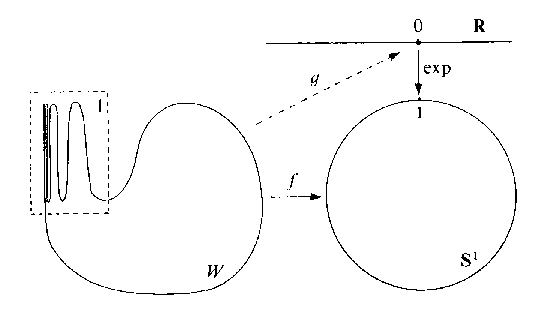
\includegraphics[width=0.7\textwidth]{figures/discont_lift.pdf}
    \caption{The map $f$ here collapses the entire ``$\sin 1/x$'' part of the space on the left into the basepoint $1$ on the circle. If a lifting map $g$ into the real line existed, then the vertical part of the ``$\sin 1/x$'' curve would have to be mapped to $0$, whereas the wiggly part would map to $1$ under $g$, making it discontinuous. From \cite[Fig.~III-6]{Bredon}.}
    \label{fig:discont_lift}
\end{figure}

\begin{thm}[Lifting Theorem]\index{Theorem!Lifting}\label{Lifting Theorem}
    Let $\pi:E\to M$ be a covering map with $\pi (p_0)=x_0$. Assume that $W$ is path-connected and locally path-connected and that $f:W\to M$ is a map with $f(w_0)=x_0$. Then a pointed map $\wt f:(W,w_0)\to (M,x_0)$ such that $\pi\circ\wt{f}=f$ exists iff $f_\ast (\pi_1(W,w_0))\subset \pi_\ast (\pi_1(E,p_0))$. Moreover, $\wt f$ is unique.
\end{thm}
\begin{proof}
    Let us construct $\wt f$ explicitly. Given $w\in W$, let $\lambda:I\to W$ be a path from $w_0$ to $w$. Then $f\circ \lambda$ is a path in $M$. Lift this to a path $\wt\lambda:(I,0)\to (E,x_0)$ and let $\wt{f}(w)=\wt{\lambda}(1)$. Then $\pi\circ \wt{f}(w)=\pi(\wt{\lambda}(1))=f(\lambda(1))=f(w)$.

    To see that $\wt{f}$ is well defined, suppose $\lambda'$ is another path in $W$ from $w_0$ to $w$ and let $\eta=(\lambda ')^{-1}$ be the reverse path from $w$ to $w_0$. Then $\lambda\bullet \eta$ is a loop based at $w_0$, and $(f\circ \lambda)\bullet (f\circ\eta)$ is a loop in $M$ based at $x_0$. Since 
    \[[f\circ\lambda \bullet f\circ\eta]=f_\ast([\lambda\bullet\eta]\in \im(f_\ast)\subset \im(\pi_\ast),\]
    $f\circ\lambda\bullet f\circ\eta$ lifts to a loop in $E$ based at $p_0$. The reverse of the portion of this lifting corresponding to $\eta$ then is a lifting $\wt{\lambda}'$ of $\lambda '$ and $\wt{\lambda}'(1)=\wt{\lambda}(1)$, as required.

    Next, we have to show that $\wt{f}$ is continuous. Let $w\in W$  and put $x=f(w)$. Let $U\subset <$ be an elementary neighborhood of $x$, and by local path-connectedness of $W$ we can let $V$ be a path-connected neighborhood of $w$ such that $f(V)\subset U$. For any point $w'\in V$ we can construct a path from $w_0$ to $w'$ by concatenating a given path $\lambda$ to $w$ with a path $\sigma$ in $V$ from $w$ to $w'$. Since $f(V)$ is contained in an elementary set, the lifting of $f\circ \sigma$ is simply $f\circ\sigma$ composed with the local inverse of $\pi$ that takes $U$ to the component of $\pi^{-1}(U)$ that contains $\wt{f}(w)$. This same component is used for all $w'\in V$ and it follows that $\wt{f}$ is continuous at $w$.

    The converse direction of the theorem follows immediately from $f_\ast=\pi_\ast\circ \wt{f}_\ast$.
\end{proof}
\begin{rem}
    Unlike in the homotopy lifting property (Theorem~\ref{homotopy lifting property}), the condition of local path connectedness for $W$ cannot be dropped here. See an example in Figure~\ref{fig:discont_lift}.
\end{rem}

\begin{cor}[{{\cite[Cor.~4.2]{Bredon}}}]\label{cor 4.2 Bredon}
    Under the conditions of the Lifting Theorem~\ref{Lifting Theorem}, if $W$ is also simply connected, then the lifting $\wt{f}$ always exists and is unique given a basepoint $p_0\in E$.
\end{cor}

\begin{cor}\label{cor homotopy groups of coverings}
    Given a covering space $E\overset{\pi}{\to}M$, there is a natural isomorphism of higher homotopy groups
    \[\pi_n(E,p_0)\cong \pi_n(M,x_0),\; n\geq 2.\]
\end{cor}
\begin{proof}
    Injectivity follows from the uniqueness of the liftings of maps $\bbS^n\to M$ into $E$. Surjectivity follows from the Lifting Theorem~\ref{Lifting Theorem} combined with the fact that $\pi_1(\bbS^n)$ is trivial for $n\geq 2$ (Corollary~\ref{cor pi_1(S^n)=0}).
\end{proof}

\begin{cor}\label{cor: homotopy groups of circle}
    $\pi_n(\bbS^1)=1$ for $n>1$.
\end{cor}
\begin{proof}
    Any map $f:\bbS^n\to \bbS^1$ lifts to $\wt{f}:\bbS^n\to \bbR $ by Corollary~\ref{cor 4.2 Bredon}. But $\wt f$ is homotopically trivial since $\bbR $ is contractible, so $f=\pi\circ\wt{f}$ is also homotopically trivial.
\end{proof}


\section{Morphisms of covering spaces}


\begin{defn}[Category of covering spaces]
The category $\mathsf{Cov}_M$ of covering spaces of a given base $M$ (say, topological covering spaces) consists of all covering spaces of $M$. The morphisms between two covering spaces $\pi$ and $\pi'$ are morphisms $f:E\to E'$ that ``map fibers to fibers'', i.e., $\pi'\circ f=\pi$, or equivalently if the following triangle commutes:
\[
\begin{tikzcd}[every matrix/.append style={name=m},   
execute at end picture={\draw [<-] ([xshift=0mm,yshift=-2mm]m-2-2.north) arc[start angle=-90,delta angle=-270,radius=0.25cm];}]
   E \arrow[rr,"f"]\arrow[ddr,swap,"\pi"]& & E'\arrow[ddl,"\pi'"]\\
   & \, & \\
   & M & \\
\end{tikzcd}
\]
\end{defn}


\begin{lem}[{{\cite[Lem.~4.4]{Bredon}}}]\label{lem 4.4 Bredon}
    Let $W$ be connected and $E$ be Hausdorff. Let $\pi:E\to M$ be a covering map and $f:W\to M$ a map. Let $\wt{f}_1,\wt{f}_2$ be two liftings of $f$ into $E$. If $\wt{f}_1(w)=\wt{f}_2(w)$ for some point $w\in W$, then $\wt{f}_1\equiv \wt{f}_2$.
\end{lem}
\begin{proof}
    Let $\wt{f}_1(w)=\wt{f}_2(w)=p$. Let $U$ be an elementary open neighborhood of $f(w)$ in $M$. Let $V$ be the component of $\pi^{-1}(U)$ containing $p$. Then $A=\wt{f}_1^{-1}(V)\cap\wt{f}_2^{-1}(V) $ is an open set in $W$ and for $a\in A$ we have $\wt{f}_1(a)=\wt{f}_2(a)$ since the homeomorphism $\pi:V\to U$ maps them both to $f(a)$. This shows that the set $\{w\in W\mid \wt{f}_1(w)=\wt{f}_2(w)\}$ is open. But this set is also closed since it is the inverse image of the diagonal under the map $\wt{f}_1\times \wt{f}_2:W\to E\times E$, and the diagonal is closed since $E$ is Hausdorff. Since $W$ is connected, this set is either empty or all of $W$.
\end{proof}
\begin{cor}[{{\cite[Cor.~4.5]{Bredon}}}]\label{cor 4.5 Bredon}
    Let $\pi_i:E_i\to M$, $i=1,2$, be covering maps such that $E_1$ is simply connected, and let $p_i\in E_i$ be such that $\pi_1(p_1)=\pi_2(p_2)$. Then there is a unique morphism of covering spaces $f:E_1\to E_2$ such that $f(p_1)=p_2$. Moreover, $f$ is a covering map.
\end{cor}
\begin{proof}
    By the Lifting Theorem~\ref{Lifting Theorem}, since $\pi_1(E_1,p_1)=1$, there is a lifting of $\pi_1\to E_1\to M$ to a map $f:E^1\to E^2$ such that $\pi_2\circ f=\pi_1$. It is unique by Lemma~\ref{lem 4.4 Bredon}.  It is an easy exercise to show that $f$ is a covering map.
\end{proof}
\begin{cor}[{{\cite[Cor.~4.6]{Bredon}}}]\label{cor 4.6 Bredon}
    If in Corollary~\ref{cor 4.5 Bredon} both $E_1$ and $E_2$ are simply connected, then the unique map $f$ is a homeomorphism.
\end{cor}
\begin{proof}
    By Corollary~\ref{cor 4.5 Bredon}, in addition to $f$ there is also an analogous map $k:E_2\to E_1$. Then $k\circ f:E_1\to E_1$ covers the identity map at $p_1$. By Lemma~\ref{lem 4.4 Bredon}, it must equal the identity everywhere. Similarly $g\circ k=\mathrm{id}_{E_2}$, hence $k=f^{-1}$.
\end{proof}

This implies that all simply connected covering spaces of a given base space $M$ are isomorphic in the category $\mathsf{Cov}_{\bullet M}$. Such covering spaces are called \emph{universal}, and are guaranteed to exist under the following mild restriction.

\begin{defn}[Locally relatively simply connected space]
    A space $X$ is locally relatively simply connected (or semilocally simply connected) if each point has a neighborhood $U$ such that all loops inside of $U$ are homotopically trivial in $X$ (i.e., for any $u\in U$ the homomorphism $\pi_1(U,u)\to \pi_1(X,u)$ is trivial).
\end{defn}

One can show that the existence of a simply connected covering space is equivalent to $M$ being locally relatively simply connected (see~\cite[Theorem~8.4]{Bredon}). Since we are mostly interested in manifolds, we will only prove the existence. Let us only work with connected, locally simply connected spaces (in particular, connected manifolds).

\begin{figure}[tp]
    \centering
    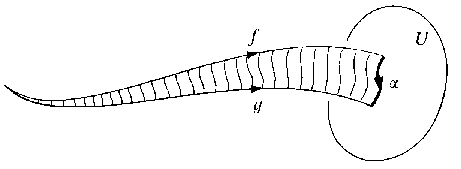
\includegraphics[width=0.5\textwidth]{figures/uni_open_set.pdf}
    \caption{Topology of the universal cover.\label{fig univ cover}}
\end{figure}

\begin{thm}[Universal cover {{\cite[Thm.~11.43]{LeeTop}}}, {{\cite[Thm.~8.4]{Bredon}}}]\index{Universal cover}
    For a given base $M$ that is a connected and \emph{locally relatively simply connected} Hausdorff space, there is a unique (up to homeomorphism) topological covering space $E\overset{\pi}{\to}M$ whose total space $E$ is simply connected. This covering space is denoted by $\wt M$ and is called the \emph{universal cover} of $M$.\index{Universal cover}
\end{thm}
\begin{proof}
    For the full proof see the references in the title. The basic idea is to explicitly construct $\wt M$ as the space of endpoints of all possible paths in $M$ based at a fixed point $m\in M$. Two paths are declared equivalent if their endpoints coincide and they are homotopic with fixed endpoints. The topology on this set of paths is introduced by considering sets of homotopic paths with endpoints belonging to an open set in $M$ (and the homotopies fix the starting point but can move the endpoint within the open set, see Figure~\ref{fig univ cover}). The projection $\pi$ maps a path to its endpoint. It is not difficult to check that this is indeed a topological covering map and the total space is simply connected. Uniqueness will follow from the universal property described below.
\end{proof}
\begin{rem}
    By examining the details of the proof one can notice that local simply-connectedness is not actually required, and semilocal simply-connectedness is sufficient. The converse direction is clear: if a loop is in an evenly covered subspace of $M$ then it lifts to $E$, and if $E$ is simply connected, the loop must be trivial in $E$. But then the composition of its homotopy to a constant loop with the covering map $\pi$ shows that the original loop in $M$ must be trivial. Thus we have shown that a connected and locally path-connected $M$ has a universal covering space iff it is locally relatively simply connected.
\end{rem}
\begin{example}
    The Hawaiian earring (Example~\ref{hawaiian earring}), as well as the infinite-dimensional torus $\bbT^\infty=\prod_{i=1}^\infty \bbS^1$, are not locally relatively simply connected, and thus don't have universal coverings.
\end{example}

\begin{thm}[{{\cite[Prop.~4.40]{Lee}}}]
Let $E\overset{\pi}{\to}M$ be a topological covering map and fix a smooth structure on $M$. Then $E$ is a topological manifold that supports a unique smooth structure such that $\pi$ is a smooth covering map with $\pi^{-1}(\partial M)=\partial E$.
\end{thm}

This theorem essentially means that in order to classify smooth covering spaces above a smooth base manifold, it suffices to only classify the topological covering spaces, and they are in one-to-one correspondence with the smooth ones. In other words, the theory of covering spaces is an intrinsically topological theory that doesn't gain or lose anything from imposing smooth structures.

\begin{cor}
For a connected smooth manifold $M$, there exists a unique simply connected smooth covering space called the universal covering manifold of $M$.
\end{cor}
From now on we won't really distinguish between smooth and topological covering spaces, although we only care about the smooth case.

Corollaries~\ref{cor 4.5 Bredon} and \ref{cor 4.6 Bredon} can now be restated in terms of morphisms:
\begin{cor}[Universality of the universal cover]\index{Universal property!of universal covers}
    \;
    \begin{enumerate}
       \item Any morphism of covering spaces is itself a covering map;
        \item If $M$ is a topological manifold (or any space that has a universal covering space), then $\wt{M}$ is the initial object in the category $\mathsf{Cov}_{\bullet M}$ of pointed covering spaces of $M$ (i.e., objects are $E\overset\pi\to M$ with a basepoint $p_0\in E$ and morphisms must respect the basepoints).
    \end{enumerate}
\end{cor}

In the category of non-pointed covering spaces, the universal cover is not an initial object, but the arrows coming out of it are unique up to automorphisms of the two covering spaces at the ends of the arrow. We now describe the sets of such automorphisms.

\section{Deck transformations}

\begin{defn}[Group action]
    An (right/left) action of a group $G$ on a set (or a space, a manifold) $X$ is a map $\Phi: G\times X\to X$, with its partial maps denoted by $\Phi_g=\Phi (g,\_):X\to X$ and $\Phi_x=\Phi(\_,x):G\to X$, such that $\Phi_e=\mathrm{id}_X$ and one of the following:\footnote{Since group actions are so ubiquitous in this book, we usually denote them by the upright $\Phi$ to distinguish from other usages of $\varPhi$.}
    \begin{align}
        \text{left action}:&& \Phi_g\circ \Phi_h&=\Phi_{gh},\\
        \text{right action}:&& \Phi_g\circ \Phi_h&=\Phi_{hg}.
    \end{align}
    In other words, right actions are the same thing as left actions on the opposite group $G^{\mathrm{op}}$. For this reason right actions are usually written as $x\cdot g=\Phi_g(x)$ and left actions as $g\cdot x=\Phi_g(x)$. The sets $G(x)=\Phi_x(G)$ are called \emph{orbits}.
\end{defn}
In the topological and smooth categories one usually considers continuous or smooth group actions, provided $G$ is a Lie group, but we will delay that discussion until \S\ref{sec: Lie group actions}. For now $G$ will always be a discrete group (i.e., a group with discrete topology), so any condition of continuity or smoothness on the action is simply a condition on each $\Phi_g$ individually.

\begin{defn}[$G$-equivariant maps]\index{Equivariant maps}\index{$G$-Set}
    The category of sets (spaces, manifolds) carrying a (left) action of $G$ is called $G\mathsf{-Set}$. Morphisms in this category are maps $f:X\to Y$ such that for all $g\in G$, $f(g\cdot x)=g\cdot f(x)$. These maps are called $G$-equivariant. Similarly, $G\mathsf{-Set}_\bullet$ consists of pointed sets with equivariant maps that respect basepoints. 
\end{defn}
\begin{defn}[Stabilizer]\index{Stabilizer}
    Given a group $G$ acting on a set $X$, and a point $x\in X$, the stabilizer of $x$ is defined as the subgroup $G_x=\{g\in G\mid \Phi(g,x)=x\}$.
\end{defn}
\begin{defn}[Transitive action]
    An action $\Phi$ is called transitive if it has only one orbit, i.e., for each pair $x,y\in X$ there is an $g\in G$ such that $\Phi(g,x)=y$.
\end{defn}
\begin{defn}[Simply transitive action]
    An action $\Phi$ is called simply transitive if for each pair $x,y\in X$ there is a \emph{unique} element $g\in G$ such that $\Phi(g,x)=y$.
\end{defn}
\begin{defn}[Faithful action]
    An action $\Phi$ is called faithful if no nontrivial elements of $G$ act trivially: $\Phi_g=\mathrm{id}_X \Leftrightarrow g=e$.
\end{defn}
\begin{defn}[Free action]
    An action $\Phi$ is called free if no nontrivial elements of $G$ have any fixed points: $\exists\,x\in X: \Phi(g,x)=x\Leftrightarrow g=e$. 
\end{defn}
\begin{prop}
    A group action is simply transitive iff it is free and transitive.
\end{prop}
\begin{proof}
    Assume a left action for simplicity. For the necessary condition, we only need to show freeness. If $\Phi_g=\mathrm{id}_X$, then $g\cdot x=x=e\cdot x$, therefore by simple transitivity $g=e$.

    For the converse, assume there are two elements such that $g_1\cdot x=g_2\cdot x=y$. Then $g_2^{-1}g_1\cdot x=x$, which means $g_2^{-1}g_1=e$ by freeness.
\end{proof}

Throughout this section, let $E\overset{\pi}{\to}M$ be a covering space with a fixed point $x_0\in M$. For simplicity, we also denote
\[G=\pi_1(M,x_0),\quad \quad F=\pi^{-1}(x_0).\]
The discrete set $F$ is called the \emph{fiber} of $\pi$ over $x_0$. We are going to describe an action of the group $G$ on $F$ as a group of permutations. 

Let $p\in F$ and let $g\in G$ be an element represented by a loop $\gamma :I\to M$. Lift it to get a map $\wt{\gamma}$ in $E$ with $\wt{\gamma}(0)=p$. Then define
\[\Phi(g,p)=p\cdot g =\tilde{\gamma}(1) \in F.\]
By Corollary~\ref{cor 3.5 Bredon} this does not depend on the choice of $\gamma$ and thus is a well-defined map $\Phi:F\times G\to F$. Now we can check some properties of this function:
\begin{enumerate}
    \item $x\cdot e=x$.
    \item $(x\cdot g)\cdot h=x\cdot (gh)$, i.e., it is a right action (because the product of two loops $gh$ corresponds to the application of $\Phi_g$ and then $\Phi_h$).
    \item $E$ is connected iff this action is transitive (i.e., there is only one orbit, $p\cdot G=F$). To see this, pick a path in $E$ from $p_0$ to another $p\in F$. This projects onto a loop $\gamma$ in $M$ and $g=[\gamma]$ provides the required element: $p_0\cdot p=p$. Conversely, if $E$ is not connected, the action is obviously not transitive.
    \item The stabilizer of a point is $G_{p_0}=\{g\in G\mid p_0\cdot g=p_0\}$. Then 
    \[
        \boxed{G_{p_0}=\im \pi_\ast=\pi_\ast(\pi_1(E,p_0))}\label{stabilizer}
    \]
    where $\pi_\ast:\pi_1(E,p_0)\to \pi_1(M,x_0)=G$ is the homomorphism induced by $\pi$. This is true because $g\in G_{x_0}$ iff $g=[\gamma]$ and $\gamma$ lifts to a loop at $p_0$, i.e., iff $g\in \im p_\ast$.
    \item Assuming $E$ is connected, the map $\phi: \ _{G_{p_0}}\bslash^{G}\to F$ taking the right coset $G_{x_0}g$ to $p_0\cdot (G_{p_0}g)=p_0\cdot g$ is a bijection.
\end{enumerate}
Obviously any covering space decomposes into a disjoint union of connected components, and the action of $\pi_1(M)$ is transitive on the fiber of each component separately. In what follows, we generally assume that $E$ is connected. In summary, we have the following theorem.
\begin{thm}
    Given a connected covering space $\pi:E\to M$, there is a one-to-one correspondence between the set $_{\pi_\ast(\pi_1(E,p_0))}\bslash^{\pi_1(M,x_0)}$ of right cosets, and the fiber $\pi^{-1}(x_0)$. (Note that $\pi_\ast(\pi_1(E,p_0))\cong \pi_1(E,p_0)$ since $\pi_\ast$ is a monomorphism by Corollary~\ref{cor 3.7 Bredon}.)
\end{thm}
\begin{cor}
    The number of sheets of a connected covering space equals the index (number of left or right cosets) of $G_{p_0}=\pi_\ast(\pi_1(E,p_0))$ in $G=\pi_1(M,x_0)$.
\end{cor}
\begin{cor}
    If $\wt\pi:\wt M\to M$ is a universal covering map (i.e., $\wt M$ is simply connected), then the number of sheets equals the order (cardinality) of the group $\pi_1(M,p_0)$.
\end{cor}

\begin{example}[Fundamental groups of real projective spaces]
    Since $\bbS^n$ is simply connected for $n>1$ and $\bbS^n$ is a double covering of the real projective space $\RP^n$, it follows that $\pi_1(\RP^n)\cong \bbZ_2$.
\end{example}

\begin{defn}[Deck transformations]\index{Deck transformations}
    For a covering space $E\overset{\pi}{\to}{M}$, consider the group $\Aut(\pi)$ of automorphisms of this covering space in the category $\mathsf{Cov}_M$ (also called \emph{deck transformations}). Its elements are homeomorphisms of $E$ that cover the identity map on $M$. For a given elementary open set $U\subset M$, they permute the connected components $U_i$ of the preimage $\pi^{-1}(U)$. In other words, the group $\mathrm{Aut}(\pi)$ acts on $E$ via morphisms of covering spaces.
\end{defn}

\begin{prop}[{{\cite[Prop.~6.2]{Bredon}}}]\label{prop 6.2 Bredon}
    If $a\in \Aut(\pi)$ and $g\in\pi_1(M,p_0)$ and $x\in \pi^{-1}(x_0)$ then $a(x)\cdot g=a(x\cdot g)$. In other words, deck transformations are equivariant w.r.t.\ the action of $\pi_1(M,x_0)$.
\end{prop}
\begin{proof}
    Let $\gamma$ be a loop at $x_0$ representing $g$ and lift it to a path $\wt\gamma$ starting at $p$. Then $\wt\gamma(1)=p\cdot g$ by definition. Look at the path $a\circ \wt{\gamma}$. It is a lifting of $\gamma$ and starts at $a(p)$. Thus is ends at $a(p)\cdot g$ by definition of the latter. But it also ends at $a(\wt\gamma(1))$, which is $a(p\cdot g)$.
\end{proof}

This proof actually shows that not only automorphisms are $G$-equivariant, but all morphisms in the category $\mathsf{Cov}_M$ are. This means that the action of $\pi_1(M)$ that we've constructed is \emph{natural}. These results can be summarized by the following theorem.
\begin{thm}[Monodromy Action]\index{Monodromy (covering spaces)}
For any covering space $E\overset{\pi}\to M$, 
\begin{enumerate}
    \item there is a natural homomorphism $\pi_1(M)\to \Aut(\pi)$ called the \emph{monodromy action};
    \item $\Aut(\wt \pi)\cong\pi_1(M)$, where $\wt\pi$ is the universal cover.
\end{enumerate}
\end{thm}

\begin{defn}[Normalizer]\index{Normalizer of a subgroup}
For a subset (not necessarily a subgroup) $H\subset G$ of a group $G$, its normalizer is 
\[\rmN_G(H)=\{n\in G\mid nH=Hn\}.\]
A subgroup $H$ is normal in $G$ iff $\rmN_G(H)=G$. Otherwise, $\rmN_G(H)$ is the largest subgroup of $G$ such that $H$ is a normal subgroup of $\rmN_G(H)$.
\end{defn}
\begin{rem}
    If $H$ is a subgroup, then $H\subset \rmN_H(H)$. Moreover, $\rmN_G(g^{-1}Hg)=g^{-1}\rmN_G(H)g$, so the normalizers of conjugate subsets are conjugate.
\end{rem}

The following lemma is the analog of the ``change of coordinates'' formulas in linear algebra: mapping the coordinates of vectors to a new basis is equivalent to conjugating the matrices representing linear operators.
\begin{lem} For any group $G$ acting on a set $X$ from the right,
\[\boxed{G_{p_0\cdot g}=g^{-1}G_{p_0}g.}\label{conjugate stabilizers}\]
Similarly, for left actions, $G_{g\cdot p_0}=gG_{p_0}g^{-1}$.
\end{lem}
\begin{proof}
    \[
        G_{p_0\cdot g}=\{h\mid (p_0\cdot g)\cdot h=p_0\cdot g\}=\{h\mid p_0\cdot ghg^{-1}=p_0\}=\{h\mid ghg^{-1}\in G_{p_0}\},
    \]
\end{proof}

The most important question in the study of deck transformations is: given two points in the fiber, when does there exist a deck transformation mapping one to the other? This is answered in the following theorem.
\begin{thm}[{{\cite[Thm.~6.3]{Bredon}}}]\label{thm 6.3 Bredon}
    Provided $E$ is connected, let $p,p_0\in F=\pi^{-1}(x_0)$, $G=\pi_1(M,x_0)$ and $G_{q}=\pi_\ast(\pi_1(E,q))$ for any $q\in E$. Then \gls{tfae}:
    \begin{enumerate}[label=(\arabic*)]
        \item $\exists\, a\in \mathrm{Aut}(\pi)$ such that $a(p_0)=p$.
        \item $\exists\, g\in \rmN_G(G_{p_0})$ such that $p_0\cdot g=p$.
        \item $G_{p_0}=G_p$.
    \end{enumerate}
\end{thm}
\begin{proof}
    Recall that $G_{p_0}=\pi_\ast(\pi_1(E,p_0))$ and $G_{p}=\pi_\ast(\pi_1(E,p))$. By the Lifting Theorem~\ref{Lifting Theorem} a map $a$ covering the identity and taking $p_0$ to $p$ exists iff $\pi_\ast(\pi_1(E,p_0))\subset \pi_\ast(\pi_1(E,p))$. Similarly, a map $a'$ covering the identity and mapping $p$ to $p_0$ exists iff the opposite inclusion holds. If both exist then $a\circ a'$ covers the identity and has a point in common with the identity, therefore $a\circ a'=\mathrm{id}_E$ by Lemma~\ref{lem 4.4 Bredon}. This proves the equivalence $(1)\Leftrightarrow (3)$.

    Now we can prove $(2)\implies(3)$: if $p=p_0\cdot g$ and $g\in \rmN_G(G_{p_0})$ then $G_p=G_{p_0\cdot g}=g^{-1}G_{p_0}g=G_{p_0}$ as claimed.

    For $(3)\implies (2)$, suppose $G_{p_0}=G_p$ and $p=p_0\cdot g$ (such a $g$ exists since $G$ acts transitively on $F$). Then $G_{p_0}=G_p=G_{p_0\cdot g}=g^{-1}G_{p_0}g$, so $g\in \rmN_G(G_{p_0})$.
\end{proof}
From $(2)\Leftrightarrow(1)$ and the last part of the proof we have the following Corollary.
\begin{cor}[{{\cite[Cor.~6.4]{Bredon}}}]\label{cor 6.4 Bredon}
    For a connected covering space, the subgroup $G_{p_0}=\pi_\ast(\pi_1(E,p_0))$ is normal in $G=\pi_1(M,x_0)$ iff the action of $\mathrm{Aut}(\pi)$ is (simply) transitive on $F=\pi^{-1}(x_0)$.
\end{cor}
\begin{cor}[{{\cite[Cor.~6.5]{Bredon}}}]\label{cor 6.5 Bredon}
    In a connected covering space, if $p$ ranges over the fiber $F$ then $G_p$ ranges over all conjugates of $G_{p_0}=\pi_\ast(\pi_1(E,p_0))$.
\end{cor}
\begin{proof}
    This is a consequence of \eqref{conjugate stabilizers}.
\end{proof}

\begin{rem}
    It is worth providing some intuition for normalizers. If two points in a $G$-set belong to the same orbit, i.e., they can be mapped into each other by some elements of $G$, then their stabilizers are obviously conjugate subgroups of $G$.

    By definition, conjugation doesn't change a normal subgroup (as a set, not pointwise). Therefore if a stabilizer of a point is normal, then all other points in that orbit have the same exact stabilizer. In particular, this means that the only elements of the group which actually move the points in the orbit are the cosets of the normal stabilizer. Moreover, if you have two group elements from the same coset of this normal stabilizer, then they act on the orbit \emph{in the exact same manner}.
\end{rem}

\begin{defn}[Regular covering map]
    A covering map $\pi$ is called regular if $\mathrm{Aut}(\pi)$ is transitive on the fiber. In the case of a connected total space this is equivalent to $G_{p_0}=\pi_\ast(\pi_1(E,p_0))$ being normal in $\pi_1(M,x_0)$.
\end{defn}

In other words, normal subgroups of $\pi_1(M,x_0)$ correspond to regular connected covering spaces of $M$. A regular covering space is one whose fundamental group ``looks the same'' in terms of the generators of $\pi_1(M,x_0)$ regardless of the choice of the basepoint $p_0$ in the fiber. Such covering spaces have an inherent ``symmetry'' given by the quotient group $G/G_{p_0}$ (which exists because $G_{p_0}$ is normal). Obviously, any regular covering space that is not connected is a disjoint union of isomorphic connected regular covering spaces. Hence, it suffices to study only the connected ones. For an example of a connected non-regular covering space, see Figure~\ref{fig:threefold-cover}.

\begin{figure}[tp]
    \centering
    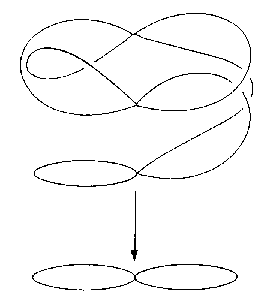
\includegraphics[width=0.4\textwidth]{figures/threefold_cover.pdf}
    \caption{This threefold cover of the figure eight space is not regular. Indeed, its group of automorphisms is trivial.}
    \label{fig:threefold-cover}
\end{figure}

\begin{rem}
    These ideas comprise the powerful \emph{Reidemeister-Schreier method} for finding presentations of subgroups $H\leq G$ given a presentation of $G$. Namely, one constructs a base space whose fundamental group is $G$, then finds a covering space corresponding to $H$ and computes its fundamental group.
\end{rem}

\begin{defn}
    Define the map $\Theta:\rmN_G(G_{p_0})\to \mathrm{Aut}(\pi)$ by $\Theta(g)=a_g$ where $a_g$ is the unique deck transformation such that $a_g(p_0)=p_0\cdot g$.
\end{defn}
\begin{thm}[Classification of Deck Transformations {{\cite[Thm.~6.8]{Bredon}}}]\label{thm 6.8 Bredon}
    $\ker \Theta=G_{p_0}$, and consequently,
    \[\mathrm{Aut}(\pi)\cong \rmN_G(G_{p_0})\slash G_{p_0}.\]
\end{thm}
\begin{proof}
    First, 
    \[a_h(a_g(p_0))=a_h(p_0\cdot g)=a_h(p_0)\cdot g=(p_0\cdot h)\cdot g=p_0\cdot (hg)=a_{hg}(p_0).\]
    This proves that $\Theta$ is a homomorphism. Next note that if $a\in \mathrm{Aut}(\pi)$ then there is an $g\in \rmN_G(G_{p_0})$ such that $a(p_0)=p_0\cdot g=a_g(p_0)$. Therefore $a=a_g$, which shows the surjectivity of $\Theta$.

    Finally we compute the kernel of $\Theta$. The result follows from the chain of equivalences
    \[a_g=\mathrm{id}_E \Leftrightarrow p_0\cdot g=p_0\Leftrightarrow g\in G_{p_0}.\]
\end{proof}
\begin{cor}
    If the covering map $E\overset{\pi}{\to} M$ is regular, then 
    \[\mathrm{Aut}(\pi)\cong G/G_{p_0}\]
\end{cor}
\begin{cor}
    If $\wt{M}\overset{\wt\pi}{\to} M$ is a universal covering map, then
    \[\mathrm{Aut}(\wt\pi)\cong G=\pi_1(M,x_0).\]
\end{cor}





\section{Classification of covering spaces}

Our examination of connected covering spaces allows us to easily prove the following classification of connected covering spaces in terms of subgroups of the fundamental group of the base.

\begin{thm}[Classification of coverings I]
    Let $M$ be path-connected, locally path-connected and semilocally simply connected so that it has a universal covering space $\wt{M}$. Then the following \emph{Galois correspondence} holds:
\begin{enumerate}
	\item The isomorphism classes of connected pointed covering spaces of $M$ are in one-to-one correspondence with subgroups of $G=\pi_1(M, x_0)$. 
	\item The isomorphism classes of connected covering spaces of $M$ without basepoints are in one-to-one correspondence with the conjugacy classes of subgroups of $G=\pi_1(M, x_0)$.
    % sets $F$ (finite or countable) with an action of the group $\pi_1(M)$ (a group action on $F$ is an element of $\Hom(\pi_1(M),G)$, where $G$ is the full permutation group of the points of $F$).
\end{enumerate}
The correspondence is given by $E\leftrightarrow \pi_\ast(\pi_1(E,p_0))=G_{p_0}$ where $\pi$ is the covering map.
\end{thm}
\begin{proof}
    The second statement follows from the first combined with Corollary~\ref{cor 6.5 Bredon}. It remains to show that the map taking a covering map with a basepoint, $\pi:(E,p_0)\to (M,x_0)$, into the subgroup $\pi_\ast(\pi_1(E,p_0))$ of $\pi_1(M,x_0)$ is a bijection. It is an injection by the Lifting Theorem~\ref{Lifting Theorem}. 
    
    To see that it is a surjection, suppose that $H\subset \pi_1(M,x_0)=G$ is a subgroup. Since $\wt{M}$ is simply connected, Theorem~\ref{thm 6.8 Bredon} gives the isomorphism $\Theta:G\to \mathrm{Aut}(\pi)$, where $\Theta(g)=a_g$. Under this map, $H$ is mapped to a subgroup $A_H\leq \mathrm{Aut}(\pi)$. Put $E=\wt{M}/A_H$ which projects to $M$ canonically. Let $p_0$ be the image of the basepoint $\wt{p}_0\in\wt{M}$. We wish to identify $\pi_\ast(\pi_1(E,p_0))$. Let $\gamma$ be a loop in $E$ at $p_0$. Lifting this to $\wt{M}$ at $\wt{p}_0$ gives the same path as a lifting of the projection of $\gamma$ to a loop at $x_0$ in $M$. Thus the lifting ends at $a_g(\wt{p}_0)$, where $g\in\pi_1(M,x_0)$ is the homotopy class of the projection of $\gamma$ to $M$. But for $\gamma$ to be a loop in $E=\wt{M}/A_H$, we must have that $\wt{p}_0$ and $a_g(\wt{p}_0)$ are in the same orbit of $A_H$. This is true iff $a_g\in A_H$, and this holds iff $g\in H$. But $g$ is an arbitrary element of $\pi_\ast(\pi_1(E,p_0))$. Thus $H=\pi_\ast(\pi_1(E,p_0))$.
\end{proof}


Now we restate the classification theorem as it was described in Example~\ref{covering category thm}. We consider all, not only connected, coverings. 

Given an action of a group $G$ on a space $X$, the space $X$ decomposes into a disjoint union of orbits of $G$. Let us assume a discrete topology on $G$, in which case a continuous/smooth action is simply one for which the maps $\Phi_g:X\to X$ are continuous/smooth for all $g$. The set of all orbits is denoted by $X\slash G$ and, if imbued with the quotient topology descended from $X$, is called the \emph{orbit space}. Note that the canonical projection $p:X\to X\slash G$ that takes a point to its orbit is open because for an open $U\subset X$, $p^{-1}(p(U))=\bigcup_g (g\cdot U)$, which is a union of open sets.

Every covering map of $M$ gives rise to an action of $G=\pi_1(M,x_0)$ on the fiber $F=F_{x_0}$. Under this action $F$ decomposes into a disjoint union of orbits $F_j$, each of them associated with a conjugacy class of stabilizer subgroups $H_j<G$. This determines a functor from the category $\mathsf{Cov}_M$ of coverings of $M$ to the category $G\mathsf{-Set}$ of sets with a left action of $G=\pi_1(M,x_0)$. (The action by path lifting is naturally a right action, so we turn it into a left one by setting $g\cdot p\coloneqq p\cdot g^{-1}$; this does not change the stabilizers.) If $F$ is a $G$-set with a transitive action of $G$, then the stabilizers of any two of its points are conjugate subgroups of $G$. Choosing $p_0\in F$ and denoting $H=G_{p_0}$, we have that $F$ is isomorphic to the set of cosets $G\slash H$, also called a \emph{homogeneous set}. From such a $G$-set $F$ we can easily reconstruct a connected covering space by taking the universal covering space $\wt{M}$, forming the quotient $\wt{M}\slash H$ by the action of $H$ (by deck transformations), and letting $\pi:\wt{M}\slash H\to M$ be the map induced by the covering map $\wt{M}\to M$. If $F$ is not homogeneous, then it is a disjoint union of homogeneous sets (orbits), and the corresponding covering space is a disjoint union of the corresponding connected ones. This provides a functor in the opposite direction. It is easy to check that these two functors are each other's quasi-inverses. We thus have the second version of the theorem.

\begin{thm}[Classification of coverings II {{\cite[Thm.~3.3.2]{tomDieck}}}]\label{covering spaces category equivalence thm}
    If $M$ admits a universal covering space, then the category $\mathsf{Cov}_M$ is equivalent to the category $\pi_1(M)\mathsf{-Set}$. The corresponding functor returns the action of $\pi_1(M)$ on the fiber of the covering space and restricts morphisms to the fiber. Its quasi-inverse reconstructs a connected component of a covering space from each orbit of the $\pi_1(M)$-set as the quotient of the universal covering by the action of the stabilizer subgroup. Similarly, $\mathsf{Cov}_{M\bullet}$ is equivalent to $\pi_1(M)\mathsf{-Set}_\bullet$.
\end{thm}

\begin{rem}
    An action of a group $G$ on a set $X$ is really a homomorphism from $G$ into the group $\mathrm{Aut}(X)$ of automorphisms (bijective mappings, a.k.a.~permutations) of $X$. Once the fiber of a covering space is identified with a fixed discrete set $F$, the action of $\pi_1(M)$ on it is an element of $\Hom(\pi_1(M),\mathrm{Aut}(F))$, called the \emph{characteristic class}\index{Characteristic class} of this covering space. A different identification of the fiber with $F$ conjugates this homomorphism by an element of $\mathrm{Aut}(F)$. Therefore, for a given discrete set $F$, the isomorphism classes of covering spaces of $M$ with fiber $F$ are in one-to-one correspondence with the conjugacy classes $\Hom(\pi_1(M),\mathrm{Aut}(F))\slash \mathrm{Aut}(F)$.
\end{rem}

The next corollary follows from the fact that the fundamental group $\pi_1$ is a homotopy invariant.
\begin{cor}
    The isomorphism classes of covering spaces of two base manifolds that are homotopy equivalent are in one-to-one correspondence. That is, the set of (isoclasses of) covering spaces is a homotopy invariant. 
\end{cor}


\begin{rem}
    Due to the path lifting property, we have a set-valued \emph{transport functor}\index{Transport functor} $T_\pi:\Pi(M)\to \mathsf{Set}$ on the fundamental groupoid that takes a path $\gamma$ in $M$, say connecting $x\in M$ to $y\in M$, and produces a map $T_\pi[\gamma]:F_x\to F_y$. Thus $T_\pi$ is an element of the category $[\Pi(M),\mathsf{Set}]$ consisting of functors from $\Pi(M)$ to $\mathsf{Set}$ and natural transformations between them. A morphism of covering spaces also induces a natural transformation between their transport functors (covariantly), therefore we have a functor $T:\mathsf{Cov}_M\to [\Pi(M),\mathsf{Set}]$. The classification theorem can be restated in yet another form: if $M$ is path-connected, locally path-connected and semilocally simply connected, then $T$ is an equivalence of categories.
\end{rem}


Now we focus on regular coverings and to each such covering associate a functor that produces other (non-regular) coverings, providing another valuable version of the classification theorem. 

\begin{defn}[Properly discontinuous action]\index{Properly discontinuous action}
    An action of a group $G$ on a space $X$ is properly discontinuous if each point $x\in X$ has a neighborhood $U$ such that $g\cdot U\cap U\neq \varnothing$ implies $g=e$.
\end{defn}
\begin{rem}
    Any properly discontinuous action is free. Indeed, suppose $g\cdot x=x$ for some $g\in G$ and $x\in X$. Then the neighborhood $U$ of $x$ guaranteed to exist by definition of a properly discontinuous action necessarily satisfies $g\cdot U\cap U\neq\varnothing$, and therefore $g=e$. Hence the action is free.
\end{rem}

\begin{defn}[$G$-principal covering]
    A right $G$-principal covering is a covering map $\pi:E\to B$ with a properly discontinuous action of $G$ on $E$ such that $\pi(p\cdot g)=\pi(p)$ for all $(g,p)\in G\times E$ and such that the induced action on each fiber is transitive.
\end{defn}

\begin{example}
    The orbit map $E\to E\slash G$ of any properly discontinuous action is a $G$-principal covering (see the proposition below). Conversely, every $G$-principal covering $\pi:E\to B$ induces a homeomorphism $\pi':E\slash G\cong B$ given by $p\cdot G\mapsto \pi(p)$. Indeed, since the action is transitive, the fiber $\pi^{-1}(x)$ coincides with the orbit $p\cdot G$ for any $p\in\pi^{-1}(x)$. Hence an inverse to $\pi'$ is given by $x\mapsto \pi^{-1}(x)=p\cdot G$. Its continuity follows from the fact that $\pi$ is a local homeomorphism.
\end{example}

We now examine the relationship between principal and regular coverings. 

\begin{prop}[{{\cite[Prop.~3.1.8]{tomDieck}}}]
    Let $\pi:E\to B$ be a covering map. Then:
    \begin{enumerate}[label=(\arabic*)]
        \item If $E$ is connected, then the action of $\Aut(\pi)$ (and any of its subgroups) is properly discontinuous.
        \item Let $B$ be locally path connected and let $H$ be a subgroup of $\Aut(\pi)$. Then the map $\pi':E\slash H\to B$ induced by $\pi$ is a covering map.
    \end{enumerate}
\end{prop}
\begin{proof}
    (1) Let $p\in E$ and $g\in \Aut(\pi)$. Let $U$ be an evenly covered neighborhood of $\pi(p)$, and let $U_p$ be the sheet over $U$ containing $p$. For $q\in U_p\cap gU_p$ we have $\pi(q)=\pi(g^{-1}q)$, since $g^{-1}$ is an automorphism. Hence $q=g^{-1}q$, since both elements are contained in $U_p$. Since a deck transformation of a connected covering with a fixed point is the identity (Lemma~\ref{lem 4.4 Bredon}), this shows $g^{-1}=e$, hence $U_p\cap gU_p=\varnothing$ for $g\neq e$, and we see that the action is properly discontinuous.

    (2) Let $U\subset B$ be open, path connected, and evenly covered. Let $\pi^{-1}(U)=\bigcup_j U_j$ be the decomposition into sheets over $U$. An element $h\in H$ permutes the sheets, since they are the path components of $\pi^{-1}(U)$. The equivalence classes w.r.t.\ $H$ are therefore open in the quotient topology of $E\slash H$ and are mapped bijectively and continuously under $\pi'$. Since $\pi$ is open, so is $\pi'$. Hence $\pi'$ is trivial over $U$. Since $B$ is locally path connected, it has an open covering by such sets $U$.
\end{proof}
\begin{cor}
    A $G$-principal covering $\pi:E\to B$ induces a homeomorphism $E\slash G\cong B$.
\end{cor}

Thus the group $\mathrm{Aut}(\pi)$ of deck transformations of any covering space $E\overset{\pi}{\to}M$ acts properly discontinuously, and if $\pi$ is regular, this action is transitive on each fiber. Therefore,
\begin{center}
    a regular covering $\pi$ is an $\Aut(\pi)$-principal covering.
\end{center}

Now we ask the opposite question: what kind of coverings can properly discontinuous actions give rise to?

\begin{prop}
    If $G$ acts properly discontinuously on a path-connected and locally path-connected Hausdorff space $E$, then the \emph{orbit map} $\pi:E\to E\slash G$ is a regular covering map with deck transformation group $\mathrm{Aut}(\pi)=G$.
\end{prop}
\begin{proof}
    Let $U\subset E$ be a path-connected open set as in the definition of properly discontinuous actions and put $U^\ast =\pi(U)$, which is open as remarked above. Since $U\to U^\ast$ is continuous, $U^\ast$ is path-connected. Also, the sets $g\cdot U$ are the components of $\pi^{-1}(U^\ast)$. The maps $g\cdot U\to U^\ast$ are continuous, open, injective and surjective, and hence homeomorphisms. Thus $\pi$ is a covering map. Elements of $G$ are deck transformations and act transitively on the fiber. There are no other deck transformations by Lemma~\ref{lem 4.4 Bredon}.
\end{proof}
\begin{cor}
    If $X$ is simply connected and locally path-connected and $G$ acts properly discontinuously on $X$, then $\pi_1(X\slash G)\cong G$.
\end{cor}


Now let $\pi$ be a $G$-principal covering with path-connected and locally path-connected $E$, so that $\pi$ induces a homeomorphism $E\slash G\cong B$, and by the above proposition, $\Aut(\pi)\cong G$. Therefore every such principal covering is regular. We conclude that
\begin{center}
    a $G$-principal covering $\pi$ with connected $E$ is a regular covering with group of deck transformations $G$.
\end{center}
(Connectedness is needed: the trivial covering $B\times G\to B$ is $G$-principal, but its group of deck transformations is the much larger group of all permutations of $G$.)


We now explain how, given a regular (or principal) covering, one can produce other coverings.

\begin{defn}[Associated covering]
    A right $G$-principal covering $\pi:E\to B$ gives rise to associated coverings. Let $F$ be a set with left $G$-action (a \emph{$G$-set}). Denote by $E\times^G F$ the quotient space $E\times F\slash \sim $ under the equivalence relation $(p,f)\sim(p\cdot g^{-1},g\cdot f)$ for $(p,f,g)\in E\times F\times G$. The continuous map $\pi_F:E\times^G F\to B$, $[p,f]\mapsto \pi(p)$ is a covering with fiber $F$ (with $F$ given the discrete topology).

    A $G$-equivariant map $\psi:F_1\to F_2$ induces a morphism of coverings
    \[\mathrm{id}_E\times^G\psi: \; E\times^G F_1\to E \times^G F_2,\; [p,f]\mapsto [p,\psi(f)].\]
\end{defn}

Thus for every right $G$-principal covering $\pi$ (over some base $B$) we have constructed the ``associated covering functor'' $A(\pi):G\mathsf{-Set}\to \mathsf{Cov}_B$ from the category of left $G$-sets (and equivariant maps) to the category of covering spaces of $B$. 

\begin{defn}[Universal $G$-principal covering]
    We call a $G$-principal covering $\pi$ \textit{universal} (among all $G$-principal coverings over all possible base spaces) if the functor $A(\pi)$ is an equivalence of categories.
\end{defn}

The classification theorem~\ref{covering spaces category equivalence thm} can now be restated as follows.
\begin{thm}[Classification of coverings III]\label{thm classification of coverings iii}
     If a covering map $\pi:E\to B$ is universal (i.e., $E$ is simply connected), then it is also universal $\pi_1(B)$-principal (i.e., the functor $A(\pi)$ is an equivalence of categories).
\end{thm}

In this sense, universal coverings are ``classifying objects'' for all other coverings. Now it is natural to ask whether the converse holds, i.e., whether every universal $G$-principal covering is the universal covering of some space $B$ such that $\pi_1(B)\cong G$. For this it suffices to show that any universal $G$-principal covering must be simply connected.

\begin{prop}
    Let $B$ be a space which admits a universal covering. If a right $G$-principal covering  $\pi:E\to B$ is universal, then $E$ is simply connected, i.e., $\pi$ is a universal covering of $B$.
\end{prop}
\begin{proof}
    First consider the group $G$ acting on itself from the left as a $G$-set. The map $[p,g]\mapsto p\cdot g$ is an isomorphism of the associated covering $A(\pi)(G)$ with $\pi$ itself. Now let $\wt{\pi}:\wt{B}\to B$ be the universal covering. By assumption, $A(\pi):G\mathsf{-Set}\to \mathsf{Cov}_B$ is an equivalence of categories, thus there exists a left $G$-set $F$ such that the covering $A(\pi)(F)$ is isomorphic to $\wt{\pi}$. An equivalence of categories preserves disjoint unions. A covering is connected iff it is not a disjoint union of two nonempty coverings, and a $G$-set is transitive iff it is not a disjoint union of two nonempty $G$-sets. Since $\wt{B}$ is connected, $F$ is therefore transitive, and since $G$ is transitive, $E$ is connected. Now pick a point $f_0\in F$. The map $g\mapsto g\cdot f_0$ is a morphism $G\to F$ in the category of $G$-sets, and applying $A(\pi)$ to it we obtain a morphism of coverings $\varphi:E\to \wt{B}$, i.e., a map such that $\pi=\wt{\pi}\circ\varphi$. Therefore $\pi_\ast(\pi_1(E,p_0))=\wt{\pi}_\ast(\varphi_\ast(\pi_1(E,p_0)))$ is trivial, since $\wt{B}$ is simply connected. But $\pi_\ast$ is injective, so $\pi_1(E,p_0)$ is trivial and $E$ is simply connected.
\end{proof}

We thus have the following abstract reformulation of the classification theorem, which will be a useful reference point for when we classify general fiber bundles.

\begin{thm}[Classification of coverings IV {{\cite[Thm.~3.4.3]{tomDieck}}}]
    A covering map $\pi:E\to B$ is universal $G$-principal for some group $G$ iff it is a universal covering map of $B$ and $G\cong \pi_1(B)$.
\end{thm}
Note that for a fixed $G$ there are many non-isomorphic universal $G$-principal coverings: the universal covering of any space $B$ whose fundamental group is $G$ will work. 

\begin{rem}\label{rem: classifying space for discrete G}
    We will later learn to construct, for any discrete group $G$, a space $X_G$ whose fundamental group is isomorphic to $G$ and which admits a universal covering. Therefore for every group $G$ there exists a universal $G$-principal covering, although it is not unique. Once we learn about $CW$-complexes we will be able to define a special universal $G$-principal covering that is unique up to homotopy (namely the universal covering of the first Eilenberg-MacLane space $\rmK(G,1)$, see \S\ref{sec: CW approx}). This fact will eventually have a natural extension to all groups and fiber bundles: for any group $G$ we will construct a so-called classifying space $\rmB G$ and a principal $G$-bundle $\rmE G\to \rmB G$ such that $\rmE G$ is contractible. There will hold isomorphisms $\pi_{n+1}(\rmB G)\cong \pi_{n}(G)$ for all $n\geq 0$. In the case of discrete $G$ the bundle $\rmE G\to \rmB G$ is obviously a covering space, and the aforementioned space $X_G$ provides a universal covering that is an ``approximation'' of this space, and for which only the first isomorphism $\pi_1(B)\cong \pi_0(G)\cong G$ holds.
\end{rem}

Since every covering space is a disjoint union of its connected components, let us separately address the classification of \emph{connected} covering spaces in terms of equivalence of certain categories. Let $\pi:E\to B$ be a universal right $G$-principal covering. A left $G$-set $F$ is a disjoint sum of its orbits. We thus have a corresponding decomposition of the total space $E\times^G F$ into the sum of $E\times^G C$, where $C$ runs over the orbits of $F$. An orbit is a transitive $G$-set and is isomorphic to a homogeneous set (set of cosets) $G\slash H$ of some subgroup $H<G$. The homeomorphism $E\times^G G\slash H\cong E\slash H$ shows that the summands $E\times^G C$ are path-connected. The action of $H$ on $E$ is properly discontinuous and therefore $E\to E\slash H$ is an $H$-principal covering. Also the induced map $\pi_H:E\slash H\to B$ is a covering.

The category of homogeneous $G$-sets and $G$-equivariant maps is called the \emph{orbit category} $\mathsf{Orb}(G)$. The sets $G\slash K$ and $G\slash L$ are isomorphic iff the subgroups $K$ and $L$ are conjugate in $G$. The stabilizers of points of $G\slash H$ are conjugate to $H$. The inclusion of the subcategory $\mathsf{Orb}(G)$ into the category of transitive $G$-sets is an equivalence.

Let $\wt{\pi}:\wt{E}\to B$ be a universal right $G$-principal covering with simply connected $\wt{E}$. Then the functor $A(\wt{\pi})$ induces an equivalence of $\mathsf{Orb}(G)$ with the category of connected coverings of $B$. Each connected covering is thus isomorphic to a covering of the form $\pi_H:\wt{E}\slash H\to B$ for a subgroup $H<G$.

Let $\pi:E\to B$ be a connected covering. The subgroup $\pi_\ast(\pi_1(E,p_0))\subset \pi_1(B,x_0)$ is called the characteristic subgroup $C(\pi,p_0)$ of $\pi$ w.r.t.\ $p_0$. Different basepoints $p_0$ lead to conjugate characteristic subgroups, and conversely, every subgroup conjugate to $C(\pi,p_0)$ arises this way. We summarize these results in the final version of the classification theorem:

\begin{thm}[Classification of coverings V {{\cite[Thm.~3.4.4]{tomDieck}}}]
    If $M$ admits a universal covering space, then the category of connected coverings of $M$ is equivalent to the orbit category $\mathsf{Orb}(\pi_1(M,x_0))$. The isomorphism class of a connected covering $\pi:E\to M$ corresponds under this equivalence to the isomorphism class of $\pi_1(M,x_0)\slash C(\pi,p_0)$ for any $p_0\in\pi^{-1}(x_0)$. The isomorphism class of a connected covering is determined by the conjugacy class of its characteristic subgroup.
\end{thm}







\section{Examples of covering spaces}

\begin{example}[Covers of $\bbS^1$ and $\mathbb{C}^\ast$]
    The example that illustrates all the basic features of this theory is $M=\bbS^1$ (which we will represent by unit complex numbers). The universal cover is clearly $\wt{M}=\bbR $ with $\wt\pi(x)=\rme^{2\pi\rmi x}$. The deck transformations of $\wt M$ consist of integer shifts $x\mapsto x+n$, $n\in \bbZ$, therefore $\Aut(\wt M)=\bbZ$. And indeed, $\pi_1(\bbS^1)=\bbZ$. This universal cover can be interpreted as a slice of the Riemann surface of the complex logarithm $w=\ln z$, since the projection on this Riemann surface is exactly $\rme^w$. In fact, the entire Riemann surface (homeomorphic to $\mathbb{C}$) itself is the universal cover of $\mathbb{C}^\ast=\mathbb{C}\setminus\{0\}$. Since $\mathbb{C}^\ast$ and $\bbS^1$ are homotopy equivalent, their covering spaces are in one-to-one correspondence.

    Furthermore, all subgroups of $\bbZ$ have the form $k\cdot \bbZ$, $k\in\mathbb{N}$. The case $k=0$ gives rise to the simply-connected universal cover with $\pi_1(\wt M)=\{0\}$. Other values of $k$ give rise to total spaces that are homeomorphic to $\bbS^1$ but the covering map is $\pi_k(\rme^{\rmi t})=\rme^{\rmi kt}$. These are the $k$-sheeted covers that can also be interpreted as slices of the Riemann surfaces of the complex roots $z^{1/k}$, since the projections on them are exactly $z^k$.
\end{example}

\begin{example}[Universal covers of graphs]
    Let $M=\varGamma$ be a connected graph with $V$ vertices and $E$ edges, i.e., a topological space consisting of $E$ copies of the interval $[0,1]$ some of which are glued to each other at their ends. Such a graph always has a maximal tree, i.e., a subgraph of $\varGamma$ that is a tree and is not contained in any other sub-tree of $\varGamma$. One can show that a maximal tree must contain all vertices of $\varGamma$. Since every tree is a contractible topological space, by retracting a maximal tree of $\varGamma$ into one point we identify all vertices of $\varGamma$ into one point. This shows that $\varGamma$ is homotopy equivalent to the wedge sum of some number of circles, each corresponding to a cycle in the graph. Namely, the number $l$ of cycles in $\varGamma$ equals the number of edges in $\varGamma$ minus the number of edges in a maximal tree of $\varGamma$. This is also equal to $1-\chi(\varGamma)$, where $\chi(\varGamma)=V-E$ is the Euler characteristic. Then by Proposition~\ref{prop computing pi1}, $\pi_1(\varGamma)$  is a free group with $l$ generators. Finally, from the above results it is easy to see that $\wt{\varGamma}$ is the \href{https://en.wikipedia.org/wiki/Cayley_graph}{Cayley graph} of this free group, i.e., the graph whose vertices are all the elements of the group, and the edges incident to a vertex correspond to the generators of the group and their inverses. The vertex on the other end of an edge is the result of the multiplication of the current vertex by the edge's generator (say, from the right). In the case of a free group with $l$ generators, this is a regular tree whose root represents the identity element and each vertex has valency/degree (number of incident edges) equal to $l$. See Fig.~\ref{Fig. Cayley} for an example of a Cayley graph.
\end{example}
\begin{figure}[tp]
    \centering
        \includegraphics[scale=0.15]{figures/Cayley.pdf}
    \caption{This graph is the universal cover of the figure eight, which is $\varGamma=\bbS^1 \vee \bbS^1$. It is also the Cayley graph of the fundamental group of $\varGamma$, i.e., the free group with two generators $a$ and $b$, $\pi_1(\varGamma)=F(\{a,b\})\cong\bbZ\ast\bbZ$. \label{Fig. Cayley}}
\end{figure}

We can now use the theory of covering spaces to prove a very important basic theorem about free groups. 
\begin{thm}[Nielsen-Schreier]\index{Theorem!Nielsen-Schreier}\label{thm Nielsen-Schreier}
    Any subgroup of a free group is free.
\end{thm}
\begin{proof}
    Let $G$ be a free group. As we've seen, it can be realized as the fundamental group of a \emph{bouquet} $M=\bigvee \bbS^1$ of as many circles as there are generators in $G$. Given a subgroup $H\leq G$, there must exist a covering space $E\overset{\pi}{\to}M$ such that $H=\pi_\ast(\pi_1(E,p_0))$ and $\pi_\ast:\pi_1(E,p_0)\to H\subset \pi_1(M,x_0)$ is an isomorphism. However, any covering space of a graph is a graph (indeed,each edge incident with a vertex in the base can be uniquely lifted to the total space, these liftings are homeomorphisms, and doing so for all vertices gives the total space a structure of a graph). In particular, any covering space of a bouquet of circles is a bouquet of circles. This implies that the fundamental group of $E$ is free, and therefore $H$ is free.
\end{proof}
\begin{cor}
    If a subgroup of a free group of finite rank has finite index, then it is also of finite rank.
\end{cor}
\begin{proof}
    Indeed, if $H\leq G$ has finite index, it can be realized as the fundamental group of a finite covering graph of a finite bouquet of circles. But any such graph has a finitely generated fundamental group.
\end{proof}
\begin{thm}[Schreier formula]
    If $G$ is a free group of finite rank $r_G$ and $H \leq G$ is a subgroup of finite index $n$, then $H$ is free of rank $r_H=n(r_G-1)+1$.
\end{thm}
\begin{proof}
    Let $G=F(x_1,\ldots,x_{r_G})$. This follows from examining the covering graph constructed in Theorem~\ref{thm Nielsen-Schreier}. It has one vertex for each right coset $Hg$ and exactly $2r_G$ edges at each vertex ($r_G$ going in and $r_G$ going out) with the outgoing edge going from $Hg$ to $Hgx_i=(Hg)\cdot x_i$ labeled by the generator $x_i$. Therefore this graph has $V=n$ vertices and $E=nr_G$ edges. The fundamental group of this graph $\wt\varGamma$ is isomorphic to $H$ and is generated by $1-\chi(\wt\varGamma)=1-V+E=n(r_G-1)+1$ loops.
\end{proof}
\begin{cor}
    Let $\varGamma$ be a covering graph of $\bigvee_{i=1}^r \bbS^1$ (with $r>1)$ that corresponds to a subgroup generated by $r'>1$ generators. If $n=(r'-1)/(r-1)$ is a positive integer then $\varGamma$ has $n$ sheets, otherwise $\varGamma$ has infinitely many sheets.
\end{cor}
\begin{cor}
    The free group of two generators, $F(a,b)$, contains free subgroups of any integer rank $r_H$. 
\end{cor}
\begin{proof}
    The set of all words whose degree (the sum of the powers of all generators in it) equals $r_H$ is one such subgroup.

    Alternatively, we can simply notice that the space $\bbS^1\vee \bbS^1$ has covering spaces that are homeomorphic to $\bigvee_{i=1}^r \bbS^1$ for any $r$.
\end{proof}

\begin{example}[Covering spaces of $\bbS^1\vee \bbS^1$]
    Consider the ``figure eight'' space $M=\bbS^1\vee \bbS^1$. Its covering spaces are in one-to-one correspondence with conjugacy classes of subgroups of the free group $F(a,b)$ of two generators (one for each circle in $M$). By Theorem~\ref{thm Nielsen-Schreier}, any subgroup of a free group is free, so each covering space of $M$ is uniquely determined by a subset of $F(a,b)$ that contains no relations (e.g., the set $\{a^2,b^2,a^2b^2\}$ is redundant and should be replaced with $\{a^2,b^2\}$). The elements of this subset generate the image of $\pi_1(E,p_0)$ under the monomorphism $\pi_\ast$.

    Some examples of these covering spaces are given in Figures~\ref{fig:sixfold covering} and \ref{fig:coverings of 8}. The covering in Figure~\ref{fig:threefold-cover} is another one. It is instructive to observe which of the coverings in Figure~\ref{fig:coverings of 8} are regular, and how the subgroups corresponding to them are normal. It is similarly instructive to verify the Lifting Theorem~\ref{Lifting Theorem}: two different covering spaces of $M$ are covering spaces of each other (say with basepoints) only if the generators of the stabilizer of one of them can be expressed in terms of the generators of the other. For example, (11) is a covering space of (1) because  $b^nab^{-n}=(b^2)^{n/2}a(b^{-2})^{n/2}$ if $n$ is even and $b^nab^{-n}=(b^2)^{(n-1)/2}bab^{-1}(b^{-2})^{(n-1)/2}$ otherwise.

    (1) and (2), up to swapping $a$ and $b$, are all of the existing connected double covers (so there are three in total). (3) and (4) are the same covering space but with different basepoints, and one can see how the corresponding subgroups are conjugates of each other by an element that connects those two points, for example $b$.
\end{example}

\begin{figure}[tp]
    \centering
    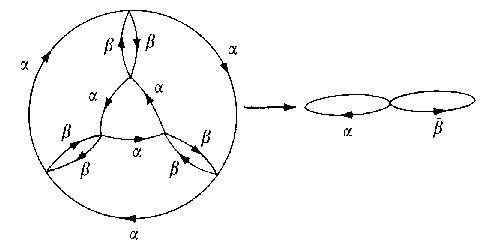
\includegraphics[width=0.6\textwidth]{figures/sixfold.pdf}
    \caption{A sixfold regular covering space of the figure eight. The fundamental group $\pi_1(E,p_0)$ is clearly generated by six loops. This makes it easy to guess that the stabilizer of any vertex is the normal subgroup of the free group $F(\alpha,\beta)$ generated by the six elements $\alpha^3,\beta^2,\left(\alpha\beta^{-1}\right)^2, \left(\alpha^{-1}\beta\right)^2, \alpha\beta^2\alpha^{-1}, \alpha^{-1}\beta^2\alpha$. To find the group of deck transformations, we factor the free group by this normal subgroup, which is equivalent to adding these six generators as relations. It is easy to check that these relations define the permutation group $\rmS_3=\langle a,b\mid a^2,b^2,ababab\rangle$. If we reversed the arrows on the inner triangle of $\alpha$'s, we'd get $\bbZ_2\times \bbZ_3$ instead. From \cite[Fig.~III-7]{Bredon}.}
    \label{fig:sixfold covering}
\end{figure}

\begin{figure}[tp]
    \centering
    \includegraphics[width=0.67\textwidth]{figures/coverings_8.pdf}
    \caption{Examples of covering spaces of the figure eight space. Each one is a graph with a marked basepoint $p_0$ such that the neighborhood of each vertex locally looks the same as in the base space: two incoming edges (labeled $a,b$) and two outgoing (also labeled $a,b$). The label of an edge indicates which generator of $\pi_1(M)$ it is projected onto by $\pi$. Next to the space is the list of the generators of the local fundamental group $\pi_1(E,p_0)$ expressed in terms of $a,b$, which means that, viewed as part of $\pi_1(M)$, they generate the stabilizer $G_{p_0}=\pi_\ast(\pi_1(E,p_0))$. The number of sheets matches the index of this subgroup. Two vertices are related by a deck transformation iff their stabilizers coincide, otherwise the stabilizers are merely conjugate. For regular coverings (1,2,5,6,7,8,9,11), all stabilizers coincide and therefore are normal. From \cite[p.~58]{Hatcher}.}
    \label{fig:coverings of 8}
\end{figure}


\begin{xca}
    Show that the covering space of the figure eight space $M=\bbS^1\vee \bbS^1$ that corresponds to the normal subgroup generated by $a^2$, $b^2$, and $(ab)^4$ (where $a,b$ are the two generators of the free group $\pi_1(M)$) is regular, and describe what it looks like. \emph{Hint:} this subgroup has index 8, so it's an eight-fold covering.
\end{xca}

\begin{xca}
    Describe the covering space of the figure eight space that corresponds to the commutator subgroup of the free group of two generators. \emph{Hint:} $F(a,b)\slash [F(a,b),F(a,b)]=\bbZ^2$, so this covering space has a $\bbZ^2$-symmetry.
\end{xca}
\begin{xca}
    Identify in $\bbS^1$ the open upper and the open lower semicircle to a point. The resulting space $X$ has four points. Show $\pi_1(X)\cong \bbZ$. Does $X$ have a universal covering?
\end{xca}
\begin{xca}
    Show that the universal cover of $M_1\times M_2$ is $\wt M_1\times \wt M_2$.
\end{xca}
\begin{xca}[{{\cite[Exercise~B.7]{Hatcher}}}]
    If $G$ is a finitely generated free group and $N$ is a nontrivial normal subgroup of infinite index, show, using covering spaces, that $N$ is not finitely generated.
\end{xca}

\begin{example}
    $\widetilde{\bbT^n}=\bbR^n$, $\widetilde{\text{SO}_3}=\text{SU}_2=\bbS^3$, $\widetilde{\text{SO}}_{n>2}=\text{Spin}_n$, $\widetilde{\text{U}_n}=\text{SU}_n\times \bbR $.
\end{example}











\clearpage
\chapter{Homotopy Theory}\label{ch homotopy theory}

\section{Homotopy groups}

\begin{defn}[Homotopy groups]\index{Homotopy groups}
Pick the base points $\bullet\in \bbS^n$ and $x_0\in X$. The set of homotopy classes of maps $\gamma:\bbS^n\to X$ such that $\gamma(\bullet)=x_0$ forms the $n$-th homotopy group $\pi_n(X,x_0)=[\bbS^n;X]_\bullet$. For two such maps, define their product by first mapping $\bbS^n$ onto the wedge sum $\bbS^n\lor \bbS^n$ via contracting an arbitrarily chosen equator (which is homeomorphic to $\bbS^{n-1}$) into one point, then apply $\gamma_1$ and $\gamma_2$ to the two hemispheres respectively, making the equator point the base point for them.

For $n=0$, $\pi_0(X)$ is defined as the set of path-connected components of $X$ (which is also the set of homotopy classes of pointed maps $\bbS^0\to X$) but does not have a natural group structure.
\end{defn}

\begin{xca}
\begin{enumerate}
    \item The above definition is consistent and the resulting homotopy classes don't in fact depend on the choice of an equator. In fact, in natural terms, this group operation is exactly the coproduct on the category of pointed spaces, given by the wedge sum $\gamma_1\lor\gamma_2:\bbS^n\lor \bbS^n\to X$ (a.k.a. \emph{concatenation}).
    \item All homotopy groups for different $x_0$ are isomorphic.
\end{enumerate}
\end{xca}


\begin{prop}[Functoriality of $\pi_n$]
    Any pointed continuous map $f:X\to Y$ induces a homomorphism of the homotopy groups $f_\ast:\pi_n(X,x_0)\to \pi_n(Y,y_0)$, and $(g\circ f)_\ast=g_\ast\circ f_\ast$. In other words, we have a \emph{functor} $\pi_n:\mathsf{Top}_\bullet\to \mathsf{Gr}$.
\end{prop}

\begin{thm}
Homotopy groups $\pi_n$, $n\geq 1$, are homotopy invariants, i.e., if $X\simeq Y$ are two homotopy equivalent path connected spaces, then $\pi_n(X,x_0)\cong\pi_n(Y,y_0)$.
\end{thm}
\begin{proof}
Exercise. Also see \cite{Hatcher}.
\end{proof}
\begin{cor}
    $\pi_n$ descends to a functor $\pi_n:\mathsf{hTop}_\bullet\to \mathsf{Gr}$ on the category $\mathsf{hTop}_\bullet$, in which the morphisms are the homotopy classes of pointed continuous maps modulo homotopy relative to the base point. In particular, homotopy equivalent spaces have isomorphic homotopy groups.
\end{cor}

\begin{thm}
For $n\geq 2$, all groups $\pi_n(X,x_0)$ are abelian.
\end{thm}
\begin{proof}
Follows from Proposition~\ref{suspension maps prop} and the fact that $\bbS^n=\Sigma\Sigma \bbS^{n-2}$ for $n\geq 2$. We have $[\bbS^n,Y]=[\Sigma\Sigma \bbS^{n-2},Y]=[\Sigma \bbS^{n-2}, \Omega Y]$, which is abelian.
\end{proof}

Another very important connection between homotopy groups and suspension will be discussed when we prove Freudenthal's Suspension Theorem~\ref{thm 6.4.7 tomDieck freudenthal}.



\section{Exact sequence of homotopy groups}

\begin{defn}[Topological triple]
    A triple $(X,A,B)$ is a topological space $X$ with a pair of subspaces $A\subset B\subset X$. When $B=\bullet$ is a point, the triple is also called a pointed pair.
\end{defn}

\begin{defn}[Relative homotopy groups]\index{Relative homotopy groups}\index{Homotopy groups!Relative}
        For a pointed pair $(X,A,\bullet)$ and $n\geq 1$ the relative homotopy group $\pi_n(X,A,\bullet)$ is the set of homotopy classes of triples $\pi_n(X,A,\bullet)=[(\bbD^n,\bbS^{n-1},\bullet);(X,A,\bullet)],$
        where $\bbD^n$ is the $n$-disk, $\bbS^{n-1}$ is its boundary, and the homotopies are through pointed maps that take $\bbS^{n-1}$ into $A$. Note that this is \emph{not} the same as homotopies relative to $\bbS^{n-1}$.
\end{defn}
These are groups with the same multiplication operation and they are still abelian for $n\geq 3$ because $[(\Sigma X,\Sigma A);(Y,B)]=[( X, A);(\Omega Y,\Omega B)]$.
\begin{prop}[Compression criterion]\label{prop: compression criterion}
    A map $f:(\bbD^n,\bbS^{n-1},\bullet)\to (X,A,\bullet)$ represents the identity in $\pi_n(X,A,\bullet)$ iff it is homotopic $\rel \partial \bbD^n\cong \bbS^{n-1}$ to a map whose image is contained in $A$.
\end{prop}
\begin{proof}
    For necessity, a map whose image is contained in $A$ can be composed with a deformation retraction of $\bbD^n$ onto the basepoint to give a homotopy to a trivial map. Conversely, if $[f]=e$ via a homotopy $H:\bbD^n\times I\to X$, then by restricting $H$ to a family of $n$-disks in $\bbD^n\times I$ starting with $\bbD^n\times \{0\}$ and ending with the disk $\bbD^n\times\{1\}\cup \bbS^{n-1}\times I$, all the disks in the family having the same boundary, then we get a homotopy from $f$ to a map onto $A$, stationary on $\bbS^{n-1}$. This is a homotopy relative to $A$.
\end{proof}

Any map $f:(X,A,x_0)\to (Y,B,y_0)$ induces maps $f_\ast :\pi_n(X,A,x_0)\to \pi_n(Y,B,x_0)$ which are homomorphisms for $n\geq 2$ and have properties analogous to those in regular homotopy: $(f\circ g)_\ast=f_\ast\circ g_\ast$, $\mathrm{id}_\ast=\mathrm{id}$, and $f_\ast=g_\ast$ if $f\sim g$ through maps of pointed pairs $(X,A,x_0)\to(Y,B,y_0)$.

In particular, the inclusions $i:(A,x_0)\hookrightarrow(X,x_0)$ and $j:(X,x_0,x_0)\hookrightarrow (X,A,x_0)$ induce such homomorphisms. Moreover, there is a third special homomorphisms that connects homotopy groups in adjacent degrees.

\begin{defn}[Boundary operator for homotopy]
    The inclusion of the boundary $\bbS^{n-1}\hookrightarrow \bbD^n$ induces restrictions of maps $f:(\bbD^n,\bbS^{n-1},s_0)\to (X,A,x_0)$ to the boundary, i.e., $\partial f=\restr{f}{\partial \bbD^n}$. For $n\geq 2$ this operator defines a homomorphism of relative homotopy groups.
\end{defn}

\begin{defn}[Exact sequence]
    Let $\calC$ be a category in which the notions of kernels and images of morphisms are well-defined. For now we assume that it is a concrete category, so kernels and images are understood as subsets of the domain and codomain, respectively. Next let there be a (finite or infinite) sequence of morphisms
    \[\cdots\to X\overset{f}{\to } Y\overset{g}{\to} Z\to \cdots \]
    We say that this sequence is exact at $Y$ if $\im f=\ker g$.
\end{defn}
\begin{example}
    In the category of pointed sets (or topological spaces etc.), kernels can be defined as the preimages of the basepoint. Exactness then amounts to $\im f=g^{-1}(*)$.

    Usually we will be concerned with the case $\calC=\mathsf{Gr}$.
\end{example}
\begin{defn}[Short exact sequence]
    A short exact sequence is a sequence of the form
    \[0\to X\overset{f}{\to } Y\overset{g}{\to} Z\to 0,\]
    where $0$ is a zero object in $\calC$.

    The exactness at $X$ is equivalent to $f$ being a monomorphism. Exactness at $Z$ is equivalent to $g$ being an epimorphism. The exactness at $Y$ essentially says that $Z\cong Y\slash \im f=Y\slash \ker g\cong Y\slash X$. In the category of groups this is just the first isomorphism theorem.
\end{defn}

\begin{example}
    If the short exact sequence is even shorter, e.g.
    \[0\to X\overset{f}{\to } Y\to 0,\]
    then its exactness is equivalent to $f$ being an isomorphism.
\end{example}

\begin{thm}[Long exact sequence of homotopy groups]\index{Long exact sequence!of homotopy groups}\label{thm long exact seq of homotopy}
    The sequence of homomorphisms
    \[\cdots \to \pi_n(A,x_0)\overset{i_\ast}{\to}\pi_n(X,x_0)\overset{j_\ast}{\to}\pi_n(X,A,x_0)\overset{\partial}{\to}\pi_{n-1}(A,x_0)\to \cdots \to \pi_0(X,x_0)\]
    is \emph{exact}. Near the end of the sequence, where the group structure is not defined, the ``kernel'' is the path-connected component of $x_0$.
\end{thm}
\begin{proof}
    In fact we will prove the long exact sequence of a pointed triple $(X,A,B,x_0)$ with $x_0\in B\subset A\subset X$:
    \begin{multline}
        \cdots \to \pi_n(A,B,x_0)\overset{i_\ast}{\to}\pi_n(X,B,x_0)\overset{j_\ast}{\to}\pi_n(X,A,x_0)\overset{\partial}{\to}\pi_{n-1}(A,B,x_0)\to \cdots \\ \to \pi_1(X,A,x_0).
    \end{multline}
    The boundary operator for triples is defined as the composition $\partial:\pi_n(X,A)\overset{\partial}{\to} \pi_{n-1}(A)\overset{i_\ast}{\to} \pi_{n-1}(A,B)$ where $i:B\hookrightarrow A$ is the inclusion map. When $B=\{x_0\}$ this reduces to the exact sequence of the pointed pair $(X,A,x_0)$, though the latter sequence continues for two more steps to $\pi_0(X,x_0)$.

    \emph{Exactness at} $\pi_n(X,B,x_0)$: First note that the composition $j_\ast\circ i_\ast$ is trivial since every map $(\bbD^n,\bbS^{n-1},s_0)\to (A,B,x_0)$ represents zero in $\pi_n(X,A,x_0)$ by the compression criterion. To see that $\ker j_\ast \subset \im i_\ast$, let $f:(\bbD^n,\bbS^{n-1},s_0)\to (X,B,x_0)$ represent the trivial element in $\pi_n(X,A,x_0)$. Then by the compression criterion again, $f$ is homotopic $\rel \bbS^{n-1}$ to a map with image in $A$, hence $[f]\in \pi_n(X,B,x_0)$ is in the image of $i_\ast$.

    \emph{Exactness at} $\pi_n(X,A,x_0)$: The composition $\partial\circ j_\ast$ is zero since the restriction of a map $(\bbD^n,\bbS^{n-1},s_0)\to (X,B,x_0)$ to $\bbS^{n-1}$ has image lying in $B$, and hence represents the trivial class in $\pi_{n-1}(A,B,x_0)$. Conversely, suppose the restriction of $f:(\bbD^n,\bbS^{n-1},s_0)\to (X,A,x_0)$ to $\bbS^{n-1}$ represents the trivial element $\pi_{n-1}(A,B,x_0)$. Then $\restr{f}{\bbS^{n-1}}$ is homotopic to a map with image in $B$ via a pointed homotopy $H:\bbS^{n-1}\times I \to A$. We can tack $H$ onto $f$ to get a new map $(\bbD^n,\bbS^{n-1},s_0)\to (X,B,x_0)$ which, as a map $(\bbD^n,\bbS^{n-1},s_0)\to (X,A,x_0)$, is homotopic to $f$ by the homotopy that tacks on increasingly longer initial segments of $H$. So $[f]\in \im j_\ast$.

    \emph{Exactness at} $\pi_n(A,B,x_0)$: The composition $i_\ast \circ \partial$ is trivial since the restriction of a map $f:(\bbD^{n+1},\bbS^n,s_0)\to (X,A,x_0)$ to $\bbS^n$ is homotopic $\rel s_0$ to a constant map via $f$ itself (via a contraction of $\bbS^n$ onto $s_0$ inside $\bbD^n$). The converse is easy if $B$ is a point, since the nullhomotopy $f_t:(\bbD^n,\bbS^{n-1})\to (X,x_0)$ of $f_0:(\bbD^n,\bbS^{n-1})\to (A,x_0)$ gives a map $F:(\bbD^{n+1},\bbS^n,s_0)\to (X,A,x_0)$ with $\partial([F])=[f_0]$. Thus the proof is finished in this case. 
    
    For a general $B$, let $f:(\bbD^{n},\bbS^{n-1},s_0)\to (A,B,x_0)$ be in the kernel of $i_\ast$ and let $F:\bbD^n\times I\to X$ be a corresponding nullhomotopy of $f$ through maps $(\bbD^n,\bbS^{n-1},s_0)\to (X,B,x_0)$. It is then clear that $F$ can be viewed as a map $\bbD^{n+1}\to X$ which restricts to $f$ on $\bbD^n\times \{0\}$, and maps the rest of the boundary into $B\subset A$, which makes $f$ the boundary of some map $(\bbD^{n+1},\bbS^n,s_0)\to (X,A,x_0)$.
\end{proof}



\section{\texorpdfstring{$CW$}{CW}-complexes}

\begin{defn}[$CW$-complex]\index{$CW$-complex}\index{Cell complex}
    A cellular structure on a set $X$ is a family $\calF $ of \textit{characteristic mappings} $f_\alpha^n:\bbD^n\to X$, where $n=0,1,2,\ldots$ and $\alpha\in A_n$ (some indexing sets), such that the following conditions hold. Let $X^{(n)}$ denote the union of images of mappings $f_\alpha^k, k\leq n$. Also $X^{(-1)}=\varnothing$.
    \begin{enumerate}
        \item For every $n$, $\bigsqcup_\alpha f_\alpha^n$ maps $\bigsqcup_\alpha \Int \bbD^n$ \emph{injectively} to $X\setminus X^{(n-1)}$. Here, we put $\Int \bbD^0=\bbD^0$.
        \item Every $f_\alpha^n$ maps $\partial \bbD^n$ to $X^{(n-1)}$.
        \item $X=\bigcup_n X^{(n)}$.
    \end{enumerate}
    
    A $CW$-complex is a Hausdorff topological space with a $CW$-structure such that the topology coincides with the final topology defined by $\calF $, also called the \emph{weak topology}\index{Weak topology}: $A\subset X$ is open iff $A\cap X^{(n)}$ is open in $X^{(n)}$ for each $n$.

    The restrictions $\partial f_\alpha^n=\restr{f_\alpha^n}{\partial \bbD^n}$ are called the \textit{attaching maps}. The subsets $X^{(n)}\subset X$ are called the $n$-skeleta of $\calF $. The images $f_\alpha^n(\bbD^n)$ are referred to as the \textit{closed cells} and $f_\alpha^n(\Int  \bbD^n)$ as \textit{open cells} (even though these are actually closed or open only as subspaces of $X^{(n)}$!). A $CW$-complex $(X,\calF )$ is said to be pointed if $X$ is pointed and the basepoint is a $0$-cell. A subcomplex is a subspace $X'\subset X$ endowed with the relative topology, together with a subfamily $\calF '\subset\calF $ such that $(X',\calF ')$ is a $CW$-complex. The highest dimension of a cell in a complex is called its dimension. A $CW$-complex is called finite if it is finite-dimensional and has a finite number of cells.
\end{defn}

We will typically work with finite $CW$-complexes, but infinite-dimensional ones will be useful as well.

\begin{rem}
The acronym $CW$ refers to the following properties.
\begin{enumerate}
    \item Closure-finiteness: every closed cell meets only finitely many open cells, which we will prove in Proposition~\ref{prop 8.1 Bredon}.
    \item Weak topology: $X$ carries the final topology defined by the family $\calF $.
\end{enumerate}
A  more general concept of cellular complexes drops these requirements. Note that, due to the inductive definition of $CW$-complexes as a collection of attaching maps, we get (C) automatically.
\end{rem}

% The following proposition shows that the weak topology induced by any \emph{finite} $CW$-structure consisting of continuous characteristic maps  on a Hausdorff space coincides with the original topology.

% \begin{prop}[{{\cite[Prop.~3.1.9]{RS2}}}]\label{prop 3.1.9 RS2}
%     Let $X$ be a Hausdorff space and let $\calF $ be a finite $CW$-structure on $X$. For $\calF $ to make $X$ into a $CW$-complex it suffices that every $f_\alpha^n\in\calF $ be continuous.
% \end{prop}
% \begin{proof}
%     We show that a subset $A \subset X$ is closed iff $(f_\alpha^n)^{-1}(A)\subset \bbD^n$ is closed for all $n$ and $\alpha$. The `only if' direction is obvious. To prove the `if' direction, assume that $(f_\alpha^n)^{-1}(A)$ is closed for all $n$ and $\alpha$. Since a continuous mapping from a compact space to a Hausdorff space is closed, it follows that $f_\alpha^n((f_\alpha^n)^{-1}(A))\subset X$ is closed for all $n$ and $\alpha$. Since $A$ is the union over all these subsets, and since their number is finite, we conclude that $A$ is closed.
% \end{proof}

Every $CW$-complex therefore can be thought of as a \emph{decomposition} of a Hausdorff space $X$ into a disjoint union of open cells of various dimensions. The space $X$, up to homeomorphism, can be inductively reconstructed from its $CW$-structure as follows. First, $X^{(0)}$ is a discrete set of points. Next, given an $(n-1)$-skeleton $X^{(n-1)}$, we can obtain $X^{(n)}$ by taking a disjoint union of $n$-disks $\sqcup_\alpha \bbD^n$ and identifying their boundaries with points of $X^{(n-1)}$ via the attaching maps $\partial f_\alpha^n:\partial \bbD^n\to X^{(n-1)}$, which are required to be continuous. The space $X$ is then the inductive union of all skeleta with the final topology.


\begin{example}
    \begin{enumerate}
        \item A graph is nothing but a $0$- or $1$-dimensional cell complex.
        \item The infinite bouquet $\bigvee_{i=1}^\infty \bbS^1$ is not a $CW$-complex because the basepoint has to meet infinitely many $1$-cells.
        \item The sphere $\bbS^n$ admits a $CW$-structure with one $0$-cell and one $n$-cell. The characteristic maps can be chosen as 
        \[f^0(*)=e_1,\quad f^n(x)=(2|x|^2-1,2\sqrt{1-|x|^2}x).\]
        Another useful $CW$-structure on the sphere has two cells in each dimension up to $n$. Its characteristic maps are
        \[f^0_\pm (*)=\pm e_1\,\quad f^k_\pm(x)=(x,\pm\sqrt{1-|x|^2},0,\ldots,0).\]
        The two $k$-cells are given by
        \[\{(x_1,\ldots,x_{k+1},0,\ldots,0)\in \bbS^n:\pm x_{k+1}\geq 0\}.\]
        \item The closed $n$-disk $\bbD^n$ has a tautological $CW$-structure with one $n$-cell. It is however sometimes convenient to have the boundary $\bbS^{n-1}$ as a subcomplex. This can be achieved by just adding either one of the two $CW$-structures of $\bbS^{n-1}$ above.
        \item The wedge sum of two $CW$-complexes $(X_1,\calF _1)\vee (X_2,\calF _2)$ carries a natural $CW$-structure $\calF _1\cup \calF _2$.
        \item The direct product $(X_1,\calF _1)\times (X_2,\calF _2)$ has a $CW$-structure with elements $(f_{1i}^n\times f_{2j}^m)\circ p_{n+m}$ where $p_{n+m}:\bbD^{n+m}\to \bbD^n\times \bbD^m$ is some chosen homeomorphism. This makes sense, because, as a homeomorphism, $p_{n+m}$ maps the boundary $\bbS^{n+m-1}$ of $\bbD^{n+m}$ onto the boundary $(\bbS^{n-1}\times \bbD^m)\cup (\bbD^n\times \bbS^{m-1})$ of $\bbD^n\times \bbD^m$. For example, the direct product of two copies of $\bbS^1$ with one cell in dimensions $0$ and $1$ yields a $CW$-structure on the torus $\bbT^2$ with one $0$-cell, one $2$-cell, and two $1$-cells. Note that in general the topology on the product complex need not coincide with the product topology, but it does when the complexes are locally finite (i.e., every point has a neighborhood that overlaps only with finitely many open cells -- such spaces are also paracompact).
    \end{enumerate}
\end{example}

\begin{prop}[{{\cite[Prop.~3.1.11]{RS2}}}]\label{prop 3.1.11 RS2}
    Let $(X,\calF )$ be a $CW$-complex, $Y$ a topological space, and $f:X\to Y$ a map. Then $f$ is continuous iff its restrictions $f\circ f_\alpha^n$ to each cell are continuous.
\end{prop}
\begin{proof}
    This is nothing but the universal property of the final topology, but let us walk through the argument. Only the sufficiency is not obvious. Let $V\subset Y$ be open. By assumption, $(f\circ f_\alpha^n)^{-1}(V)$ is open in $\bbD^n$ for all $n$ and $\alpha$. Since $(f\circ f_\alpha^n)^{-1}(V)=(f_\alpha^n)^{-1}(f^{-1}(V))$, then $f^{-1}(V)\subset X$ is open by virtue of being the image of an open set under a quotient map (and all quotient maps are open by definition). 
\end{proof}

% \begin{prop}[{{\cite[Prop.~3.1.12]{RS2}}}]\label{prop 3.1.12 RS2}
%     Let $(X,\calF )$ be a $CW$-complex, $Y$ a topological space, and $f_n:X^{(n)}\to Y,n=0,1,\ldots$ a family of continuous mappings satisfying $\restr{f_{n+1}}{X^{(n)}}=f_n$ for all $n$. Then there exists a unique mapping $f:X\to Y$ that restricts to $f_n$ on $X^{(n)}$ for all $n$, and $f$ is continuous.
% \end{prop}
% \begin{proof}
%     Since the assumption implies that $\restr{f_{m}}{X^{(n)}}=f_n$ for all $m>n$, and since $X$ is the union of $n$-skeleta, we can define $f$ by $\restr{f}{X^{(n)}}=f_n$. Uniqueness is then obvious. To check continuity, observe that for all $n,i$ and $x\in \bbD^n$, we have $f(f_i^n(x))=f_n(f_i^n(x))$. It follows that $f\circ f_i^n$ is continuous for all $n$ and $i$ and hence, by Proposition~\ref{prop 3.1.11 RS2}, that $f$ is continuous.
% \end{proof}

\begin{prop}[{{\cite[Prop.~8.1]{Bredon}}}]\label{prop 8.1 Bredon}
    If $X$ is a $CW$-complex then
    \begin{enumerate}[label=(\arabic*)]
        \item if $A\subset X$ has no two points in the same open cell, then $A$ is closed and discrete;
        \item if $K\subset X$ is compact then $K$ is contained in a finite union of open cells;
        \item each cell of $X$ is contained in a finite subcomplex of $X$ (i.e., the cell complex is \emph{``closure finite''}).
    \end{enumerate}
\end{prop}
\begin{proof}
    We will first show that all three statements are equivalent to each other.
    
    $(1)\implies (2)$. If $K\subset X$ is compact then let $A\subset K$ be a set of points, one from each open cell touching $K$. By (1) $A$ is closed, hence compact, and discrete. Hence $A$ is finite. But that means $K$ is contained in a finite union of open cells as claimed.

    $(2)\implies(3)$. In fact, for a cell $\alpha$, we will only use (2) for the set $K$ which is the image of the attaching map $f_{\partial \alpha}:\partial \bbD^n\to X^{(n-1)}$ of that cell, and the images of attaching maps of smaller-dimensional cells. Statement (2) implies that $X_\sigma=f_\sigma(\bbD^n)$ is contained in a finite union of open cells, and by construction all of these are of smaller dimension except for $U_\sigma=f_\sigma(\Int \bbD^n)$ itself. By the same token each of these lower-dimensional closed cells is contained in a finite union of open cells of even lower dimension (except for open the cell itself), and so on. This reasoning obviously must come to an end with $0$-cells in a finite number of steps, and, at that stage, the union of the cells produced a finite subcomplex.

    $(3)\implies(1)$. Consider the intersection of $A$ with a closed cell. By (3) this is contained in a finite subcomplex. Since $A$ has at most one point in common with any open cell this intersection must be finite, and hence closed. For any point $x\in A$, the set $A\setminus\{x\}$ satisfies the hypothesis for $A$, and so it must also be closed. Hence $\{x\}$ is open in $A$, so $A$ is discrete.

    Finally, we put all this together. Statement (1) clearly holds for $X^{(0)}$ (it must be discrete because it has the final topology of maps of points). Suppose we know (1) for the $n$-skeleton $X^{(n)}$. Then we also have (2) for $X^{(n)}$. In turn, we get (3) for $X^{(n)}$. But the proof of $(2)\implies(3)$ for a particular $k$-cell only used (2) for subsets of $X^{(k-1)}$. Thus we actually have (3) for $X^{(n+1)}$. Thus we also have (1) for $X^{(n+1)}$. Consequently, we have all three statements for $X^{(n)}$ for all $n$. But any cell is in some $X^{(n)}$, and so we know (3) for $X$ itself, and this implies (1) then (2) for $X$.
\end{proof} 
\begin{cor}
    The boundary of each cell is contained in finitely many closed cells of lower dimensions.
\end{cor}

\begin{thm}[{{\cite[Thm.~8.2]{Bredon}}}]\label{thm 8.2 Bredon}
    A compact subset of a $CW$-complex is contained in a finite subcomplex.
\end{thm}
\begin{proof}
    Let $K\subset X$ be compact. By (2) of Proposition~\ref{prop 8.1 Bredon}, $K$ is contained in a union of a finite number of open cells. By (3) of the same Proposition, each of these is contained in a finite subcomplex. The union of this finite number of finite subcomplexes is a finite subcomplex containing $K$.
\end{proof}

\begin{cor}\label{cor direct limit of pi_n for CW}
    If $X_1\hookrightarrow X_2\hookrightarrow \cdots$ is an infinite sequence of inclusions of $CW$-subcomplexes, then 
    \[\pi_n(\colimit X_i)=\colimit \pi_n(X_i).\]
\end{cor}
\begin{proof}
    Let $X=\colimit X_i=\bigcup X_i$ be the limiting $CW$-complex. Since $\bbS^n$ is compact, its continuous image in $X$ under any representative of an element of $\pi_n(X)$ is compact and thus contained in a finite subcomplex. Therefore every element of $\pi_n(X)$ is contained in $\pi_n(X_k)$ for some $k$ and hence in the directed colimit $\colimit \pi_n(X_i)$. Conversely, every element of this colimit is represented by some element of $\pi_n(X_k)$ for some $k$ by the explicit construction of the colimit.
\end{proof}




\begin{prop}
    A $CW$-complex is locally compact (every point has an open neighborhood contained in a compact set) iff it is locally finite (every point has an open neighborhood contained in a finite union of cells).
\end{prop}
\begin{proof}
    Exercise.
\end{proof}



\begin{defn}[Directed system, Directed colimit]\index{Direct limit!see {Directed colimit}}\index{Directed colimit}\label{def directed system}\index{Directed system}
    A directed system of topological spaces consists of a directed set $(A,\leq)$ (a poset such that for all $a,b\in A$ there exists $c\in A$ such that $a\leq c$ and $b\leq c$), a topological space $X_\alpha$ for every $\alpha \in A$ and a continuous mapping $f_{\beta\alpha}:X_\alpha\to X_\beta$ for every pair $\alpha\leq\beta$ such that $f_{\alpha\alpha}=\id_{X_\alpha}$ and $f_{\gamma\beta}\circ f_{\beta\alpha}=f_{\gamma\alpha}$ for all $\alpha\leq\beta\leq \gamma$. The \emph{colimit indexed by a directed category}, or just the directed colimit (historically \emph{direct limit})
    \[X=\colimit X_\alpha\]
    of the directed system $\{X_\alpha,f_{\beta\alpha}\}$ is (up to homeomorphism) the topological quotient of the disjoint union $\bigsqcup_{\alpha\in A} X_\alpha$ w.r.t.\ the equivalence relation that $x\in X_\alpha$ is equivalent to $y\in X_\beta$ iff $\gamma\in A: f_{\gamma\alpha}(x)=f_{\gamma\beta} (y)$. Composition of the natural inclusions $X_\alpha\hookrightarrow \bigsqcup_\alpha X_\alpha$ with the quotient map yields continuous mappings
    \[\varphi_\alpha:X_\alpha\to X\]
    and the topology of $X$ coincides with the final topology defined by these maps. That is, a subset of $X$ is open iff its preimage under $\varphi_\alpha$ is open in $X_\alpha$ for all $\alpha$. In other words, the directed colimit space is the set-theoretic directed colimit with the final topology for the maps $\varphi_{\alpha}$.
\end{defn}

Directed colimits are nothing but a generalization of pushouts to infinite families of objects, and will come up again in a more general categorical setting when we discuss homological algebra. Historically they are called \emph{direct limits}, but we avoid this nomenclature due to its proneness to confusion. A much more complete investigation of directed colimits will be done in \S\ref{Limits and colimits}.


\begin{prop}[{{\cite[Prop.~3.1.14]{RS2}}}]\label{prop 3.1.14 RS2}
    Let $\{X_\alpha,f_{\beta\alpha}\}$ and $\{Y_\alpha,g_{\beta\alpha}\}$ be directed systems of topological spaces over the same index set $A$ and let $X$ and $Y$, respectively, be the directed colimits. Every family of continuous mappings $h_\alpha:X_\alpha\to Y_\alpha$ satisfying $h_\beta \circ f_{\beta\alpha}=g_{\beta\alpha}\circ h_\alpha$ whenever $\alpha\leq \beta$ descends to a continuous mapping $h:X\to Y$.
\end{prop}

\begin{prop}[{{\cite[Prop.~3.1.15]{RS2}}}]\label{prop 3.1.15 RS2}
    Let $\{X_\alpha,f_{\beta\alpha}\}$ be a directed system of topological spaces and let $X$ be the directed colimit. If for some $i$ one has $\pi_i(X_\alpha)=0$ for almost all (i.e., all but finitely many) $\alpha$, then $\pi_i(X)=0$.
\end{prop}


\begin{thm}[$CW$ Construction Theorem {{\cite[Thm.~5.20]{LeeTop}}}]
    Suppose $X_0\subset X_1\subset\cdots \subset X_{n}\subset $ is a sequence of topological spaces satisfying the following conditions:
    \begin{enumerate}[label=(\roman*)]
        \item $X_0$ is a nonempty discrete space.
        \item For each $n\geq 1$, $X_n$ is obtained from $X_{n-1}$ by attaching a (possibly empty) collection of $n$-cells.
    \end{enumerate}
    Then $X=\bigcup_n X_n$ has a unique topology coherent with the family $\{X_n\}_n$ (i.e., it is the final topology for the inclusions $X_n\hookrightarrow X$), and a unique cell decomposition making it into a $CW$-complex whose $n$-skeleton is $X_n$ for each $n$.
\end{thm}
\begin{proof}
    The uniqueness of the topology coherent with $\{X_n\}_n$ and of the cell decomposition is practically obvious. Finally, in the case of infinitely many cells one needs to check that $X$ is closure-finite and has the weak topology. See {{\cite[Thm.~5.20]{LeeTop}}} for full details.
\end{proof}

\begin{cor}
    The family of skeleta $X^{(k)}$ of a $CW$-complex together with the natural inclusion maps $f_{lk}:X^{(k)}\hookrightarrow X^{(l)}$ for $k\leq l$ forms a directed system of spaces. The directed colimit of this system is homeomorphic to $X$: 
    \[X\cong \colimit X^{(n)}.\]
\end{cor}


\begin{example}[$\bbR^\infty$]\index{$\bbR^\infty$}\label{R-infty}
    By including $\bbR^n\hookrightarrow \bbR^{\bbN }$ via $x=(x_1,\ldots,x_n)\mapsto (x_1,\ldots,x_n,0,0,\ldots)$, we can take the directed colimit
    \[\bbR^\infty=\colimit \bbR^n.\]
    This space consists of sequences of reals with only finitely many nonzero elements. The final topology on this space is strictly finer than the subspace topology inherited on it from the direct product topology on $\bbR^{\mathbb{N}}$.\footnote{The direct product topology on $\prod_\alpha X_\alpha$ is the coarsest topology under which the natural projections $\prod_\alpha X_\alpha\overset{\mathrm{pr}_\alpha}{\to} X_\alpha$ are continuous, and it is generated by sets of the form $\prod_\alpha U_\alpha$ where $U_\alpha\subset X_\alpha$ is open and for almost all $\alpha$, $U_\alpha=X_\alpha$.} In fact, $\bbR^\infty$ itself is not open as a subset of $\bbR^{\mathbb{N}}$.
\end{example}

\begin{example}[$\bbS^\infty$]\index{$\bbS^\infty$}\label{S-infty}
    Since we can obtain $\bbS^n$ from $\bbS^{n-1}$ by attaching two cells, we can take the directed colimit
    \[\bbS^\infty=\colimit \bbS^n.\]
    This space includes every sphere $\bbS^n$ as a subcomplex. By the above theorem, $\pi_n(\bbS^\infty)=0$ for all $n$, however let us show the stronger result that $\bbS^\infty$ is contractible.

    The space $\bbR^\infty$ has a norm inherited from Euclidean norms on $\bbR^n$, which is simply $|x|=\sqrt{\sum_{i=1}^\infty x_i^2}$. The unit sphere under this norm is clearly a union of regular finite-dimensional spheres embedded into each other at the equator, which is $\bbS^\infty$. First, define the homotopy $f_t:\bbR^\infty\to \bbR^\infty$ by 
    \[f_t(x)=(1-t)x+tTx,\label{eq contracting homotopy S-inf}\]
    where $T(x_1,x_2,\ldots)=(0,x_1,x_2,\ldots)$ is the shift operator. This $f_t$ takes nonzero vectors to nonzero vectors for all $t\in[0,1]$, therefore $f_t/|f_t|$ restricts to a homotopy from $\id_{\bbS^\infty}$ to $Tx$ on $\bbS^\infty$. Then a homotopy from this map to a constant map is given by $g_t/|g_t|$ where
    \[g_t(x)=(1-t)Tx+te_1,\]
    where $e_1=(1,0,0,\ldots)$ is the basepoint.
\end{example}



\begin{example}[$CW$-structures of projective spaces]\label{example CW structures of projective spaces}
    The projective space $\RP^n$  is defined as the space of all lines through the origin in $\bbR^{n+1}$, i.e., the topological quotient of
    $\RP^n\setminus \{0\}$ under the identifications $v\sim\lambda v$ for all $v\in \bbR^{n-1}\setminus \{0\}$ and $\lambda\neq 0$. We can restrict to vectors of length $1$, so it becomes the quotient space $\bbS^n\slash(v\sim -v)$. This is equivalent to the quotient of a hemisphere $\bbD^n$ with antipodal points of $\partial \bbD^n$ identified. Since $\partial \bbD^n$ with antipodal points identified is just $\RP^{n-1}$, we see that $\RP^n$ is obtained from $\RP^{n-1}$ by attaching an $n$-cell, with the quotient map $\bbS^{n-1}\to \RP^{n-1}$ as the attaching map. It follows by induction on $n$ that $\RP^n$ has a cell complex structure $e^0\cup e^1\cup \cdots \cup e^n$ with one cell $e^i$ in each dimension $i\leq n$.

    As a consequence, the infinite union $\RP^\infty=\bigcup_n \RP^n$ becomes a cell complex with one cell in each dimension. We can view $\RP^\infty$ as the space of lines through the origin in $\bbR^\infty$.

    Similarly, it is possible to obtain $\CP^n$, the space of complex lines through the origin in $\bbC^{n+1}$, as the quotient of the disk $\bbD^{2n}$ under the identifications $v\sim\lambda v$ for $v\in\partial \bbD^{2n}$ and $|\lambda|=1$, in the following way. The vectors in the unit sphere $\bbS^{2n+1}\subset\bbC^{n+1}$ with last coordinate real and nonnegative are precisely the vectors of the form $(w,\sqrt{1-|w|^2})\in\bbC^n\times \bbC$ with $|w|\leq 1$. Such vectors form the graph of the function $w\mapsto \sqrt{1-|w|^2}$. This is a disk $\bbD^{2n}_+$ bounded by the sphere $\bbS^{2n-1}\subset \bbS^{2n+1}$ consisting of vectors $(w,0)\in\bbC^n\times\bbC$ with $|w|=1$. Each vector in $\bbS^{2n+1}$ is equivalent under the identifications $v\sim\lambda v$ to a vector in $D_+^{2n}$, and the latter vector is unique if its last coordinate is nonzero. If the last coordinate is zero, we have just the identifications $v\sim\lambda v$ for $v\in \bbS^{2n-1}$.

    From the description of $\CP^n$ as the quotient of $\bbD^{2n}_+$ under the identifications $v\sim\lambda v$ for $v\in \bbS^{2n-1}$ it follows that $\CP^n$ is obtained from $\CP^{n-1}$ by attaching a cell $e^{2n}$ via the quotient map $\bbS^{2n-1}\to \CP^{n-1}$. So by induction on $n$ we obtain a cell structure $\CP^n=e^0\cup e^2\cup\cdots \cup e^{2n}$ with cells only in even dimensions. Similarly, $\CP^\infty$ has a cell structure with one cell in each dimension.
\end{example}




\begin{thm}[{{\cite[Thm.~5.22]{LeeTop}}}]
    Every $CW$-complex is paracompact.
\end{thm}
\begin{proof}
    It suffices to show that any open covering $\{U_\alpha\}_\alpha$ of the complex $X$ supports a subordinate \gls{pou} (since part of the definition of a \gls{pou} is that only finitely many of the functions $\chi_\alpha$ have nonzero values at a given point). It can be constructed inductively by extending a \gls{pou} from the $n$-skeleton to the $(n+1)$-skeleton, extending each function cell by cell.
    
    A full proof can be found in \cite[Thm.~5.22]{LeeTop}, but one needs to include the corrections from the book's \href{https://sites.math.washington.edu//~lee/Books/ITM/errata.pdf}{errata list}. 
\end{proof}

\begin{prop}[{{\cite[Prop.~5.23]{LeeTop}}}]
    Suppose $X$ is a $CW$-complex with countably many cells. If $X$ is locally Euclidean, then it is a topological manifold.
\end{prop}
\begin{proof}
    Every $CW$-complex is Hausdorff by definition. Further, $X$ is a quotient of a disjoint union of countably many disks of various dimensions. Such a disjoint union is easily seen to be second countable. One then uses the general fact that quotient maps preserve second countability (it is enough to check the existence of a finite subcover for any cover by coordinate balls, because each coordinate ball is second countable and a union of countably many such sets has to be as well). We conclude that $X$ is second countable, and thus a manifold.
\end{proof}




\section{Homotopy extension}\label{sec: homotopy extension}

\begin{defn}[Homotopy Extension Property]\index{Homotopy Extension Property}\label{HEP}
    A continuous map $i:A\to X$ is said to have the homotopy extension property w.r.t.\ a space $Y$ if any homotopy $F:A\times I\to Y$ of a given map $F_0:A\to Y$ can be extended to a homotopy $\wt{F}:X\times I\to Y$ with any given initial condition $\wt{F}_0$.
    In other words, we are looking for a continuous map $\wt F$ that makes the following diagram commute:
    \[
    \begin{tikzcd}[every matrix/.append style={name=m}, row sep=large, column sep=large]
       Y & X\arrow[l,"\wt F_0",swap]\arrow[dl,"\wt F",dashed,swap]\\
       Y^I \arrow[u,"e_0"]  & A. \arrow[u,"i",swap]\arrow[l,"F"]
    \end{tikzcd} \label{HEP diagram}
    \]
    Here, $e_0$ is the evaluation map $\gamma\in Y^I\mapsto \gamma(0)\in Y$.

    A topological pair $(X,A)$ is said to have the \gls{hep} w.r.t.\ $Y$ if the inclusion map $i:A\hookrightarrow X$ does.
\end{defn}

\begin{defn}[Cofibration]
    If a map $i:A\hookrightarrow X$ satisfies the \gls{hep} for any space $Y$, it is called a cofibration.
\end{defn}

Obviously an inclusion $i:A\hookrightarrow X$ satisfies the \gls{hep} if every pair of maps $X\times\{0\}\to Y$ and $A\times I\to Y$ that agree on $A\times \{0\}$ can be extended to a map $X\times I\to Y$.

\begin{lem}
    A pair $(X,A)$ is a cofibration iff $(X\times\{0\})\cup( A\times I)$ is a retract of $X\times I$.
\end{lem}
\begin{proof}
    For one direction, the \gls{hep} for $(X,A)$ implies that the identity map on $(X\times\{0\})\cup (A\times I)$ extends to a map $X\times I\to (X\times\{0\})\cup (A\times I)$, which makes $(X\times\{0\})\cup (A\times I)$ a retract of $X\times I$.

    The converse is equally easy when $A$ is closed in $X$. Indeed, then any two maps $X\times\{0\}\to Y$ and $A\times I\to Y$ that agree on $A\times\{0\}$ combine to give a map $X\times\{0\}\cup A\times I\to Y$ which is continuous since it is continuous on those two closed sets separately. By composing this map with a retraction $X\times I\to X\times\{0\}\cup A\times I$ we get an extension $X\times I\to Y$. 

    The hypothesis that $A$ is closed can be avoided by a more complicated argument, see~\cite[Prop.~A.18]{Hatcher}. For Hausdorff spaces $X$ this is not needed, since if $(X\times\{0\})\cup (A\times I)$ is a retract of $X\times I$ and $X$ is Hausdorff, then $A$ must in fact be closed in $X$. Indeed, if $r:X\times I\to X\times I$ is a retraction onto $(X\times\{0\})\cup (A\times I)$, then the image of $r$ is the set of points $z\in X\times I$ with $r(z)=z$, a closed set if $X$ is Hausdorff, so $(X\times\{0\})\cup (A\times I)$ is closed in $X\times I$ and hence $A$ is closed in $X$.
\end{proof}

The case of Hausdorff $X$ will suffice for our needs, so the above proof is complete as far as we are concerned.

\begin{example}
    A simple example of a pair $(X,A)$ with $A$ closed for which the \gls{hep} fails is the pair $(I,A)$ where $A=\{0,1,\frac12,\frac13,\frac14,\ldots\}$. There is no continuous retraction $I\times I\to (I\times\{0\})\cup (A\times I)$. The breakdown of homotopy extension here can be attributed to the bad structure of the pair near $0$.
\end{example}

\begin{figure}[tp]
    \centering
    \includegraphics[width=0.5\textwidth]{figures/cylinder.pdf}
    \caption{Mapping cylinder of $f$.}
    \label{fig:mapping cyl}
\end{figure}

Recall from \S\ref{sec.homotopy} the mapping cylinder\index{Mapping cylinder} $Z_f$ of a map $f:X\to Y$, see Figure~\ref{fig:mapping cyl}: it is the quotient of $(X\times I)\sqcup Y$ that identifies $(x,0)\in X\times I$ with $f(x)\in Y$. We will now need its description as a pushout:
    \[
    \begin{tikzcd}[every matrix/.append style={name=m}, row sep=large, column sep=large]
       X \sqcup X\arrow[r,"f\sqcup \mathrm{id}"]\arrow[d,"i_0\sqcup i_1",swap] & Y\sqcup X\arrow[d,"s\sqcup j"]\\
       X\times I \arrow[r,"a", swap] & Z_f
    \end{tikzcd} \quad
    \begin{matrix}
        Z_f=\bigslant{(X\times I)\sqcup Y}{(x,0)\sim f(x)},\\
        s(y)=y,\; j(x)=(x,1), \\ i_0(x)=(x,0),\; i_1(x)=(x,1).
    \end{matrix}
    \]
We also have the projection $q:Z_f\to Y$, $(x,t)\mapsto f(x)$, $y\mapsto y$.

The images $j(X)$ and $s(Y)$ are homeomorphic to $X$ and $Y$ respectively. When $f$ is a homotopy equivalence, both of these subspaces of $Z_f$ can be shown to be deformation retracts of $Z_f$. Therefore two spaces $X,Y$ are homotopy equivalent iff they are homeomorphic to deformation retracts of some third space $Z$. See, e.g., \cite[Prop.~7.46]{LeeTop} for a proof. We will also provide a proof in Corollary~\ref{cor 0.21 Hatcher}.


\begin{figure}[tp]
    \centering
    \includegraphics[width=0.3\textwidth]{figures/hep_example.pdf}
    \caption{Mapping cylinder neighborhood from Example~\ref{example Z_f hep}.}
    \label{fig: Z_f hep}
\end{figure}
\begin{example}\label{example Z_f hep}
    A pair $(X,A)$ has the \gls{hep} if $A$ has a mapping cylinder neighborhood of $X$, by which we mean a closed neighborhood $N$ containing a subspace $B$, thought of as the boundary of $N$, with $N\setminus B$ an open neighborhood of $A$, such that there exists a map $f:B\to A$ and a homeomorphism $h:Z_f\to N$ with $\restr{h}{A\cup B}=\id$. Mapping cylinder neighborhoods like this occur fairly often. For example thickened graphs in the plane, see Figure~\ref{fig: Z_f hep}.
\end{example}

\begin{xca}
    Show that the mapping cylinder of the double covering map $\pi$ of the circle $\bbS^1$ ($\pi(z)=z^2$ on the unit circle in $\bbC$) is homeomorphic to a bounded M\"obius band.
\end{xca}


\begin{prop}[{{\cite[Prop.~0.16]{Hatcher}}}]\label{prop 0.16 Hatcher}
    If $(X,A)$ is a $CW$ pair (i.e., $A$ is a subcomplex of $X$), then $(X\times\{0\})\cup (A\times I)$ is a deformation retract of $X\times I$, hence $(X,A)$ is a cofibration.
\end{prop}
\begin{proof}
    There is a retraction $r:\bbD^n\times I\to (\bbD^n\times\{0\})\cup (\partial \bbD^n\times I)$, for example the radial projection from the point $(0,2)\in \bbD^n\times \bbR$. Then setting $r_t=t\cdot r+(1-t)\id$ gives a deformation retraction of $\bbD^n\times I$ onto $(\bbD^n\times\{0\})\cup (\partial \bbD^n\times I)$. This deformation gives rise to a deformation retraction of $X^{(n)}\times I$ onto $(X^{(n)}\times\{0\})\cup ((X^{(n-1)}\cup A^{(n)})\times I)$ since $X^{(n)}$ is obtained from the latter by attaching copies of $\bbD^n\times I$ along $(\bbD^n\times\{0\})\cup (\partial \bbD^n\times I)$. If we perform this deformation retraction in dimension $n$ during the $t$-interval $[2^{-n-1},2^{-n}]$, this infinite concatenation of homotopies is a deformation retraction of $X\times I$ onto $(X\times\{0\})\cup (A\times I)$. There is no problem with continuity of this deformation at $t=0$ since it is continuous on $X^{(n)}\times I$, being stationary there during the $t$-interval $[0,2^{-n-1}]$, and $CW$-complexes have the weak topology w.r.t.\ their skeleta so a map is continuous iff its restriction to each skeleton is continuous.
\end{proof}

\begin{prop}[{{\cite[Prop.~0.17]{Hatcher}}}]
    If the pair $(X,A)$ is a cofibration and $A$ is contractible, then the quotient map $q:X\to X\slash A$ is a homotopy equivalence.
\end{prop}
\begin{proof}
    We can use the \gls{hep} to extend a contraction of $A$ to a homotopy of maps $X\to X$ that map $A$ to $A$. This descends to a homotopy of maps $X\slash A\to X\slash A$. At $t=1$ this homotopy produces a map that maps $A$ to the point to which $A$ was contracted, so this map induces a map $X\slash A\to X$. It is then easy to see that this map is a homotopy inverse of $q$ via the two homotopies constructed above.
\end{proof}

\begin{prop}[{{\cite[Prop.~0.18]{Hatcher}}}]
    If $(X_1,A)$ is a $CW$-pair and we have the attaching maps $f,g:A\to X_0$ that are homotopic, then $X_0\sqcup_f X_1\simeq X_0\sqcup_g X_1 \rel X_0$.
\end{prop}
\begin{proof}
    If $F:A\times I\to X_0$ is the homotopy from $f$ to $g$, then consider the space $X_0\sqcup_F (X_1\times I)$. This contains both spaces in the claim of the theorem as subspaces. A deformation retraction of $X_1\times I$ onto $(X_1\times \{0\})\cup (A\times I)$ as in Proposition~\ref{prop 0.16 Hatcher} induces a deformation retraction of $X_0\sqcup_F (X_1\times I)$ onto $X_0\sqcup_f X_1$. Similarly that space retracts onto $X_0\sqcup_g X_1$. Both of these deformation retractions restrict to the identity map on $X_0$, so they give the necessary homotopy equivalence.
\end{proof}

\begin{prop}[{{\cite[Prop.~0.19]{Hatcher}}}]
    Suppose $(X,A)$ and $(Y,A)$ are cofibrations and $f:X\to Y$ is a homotopy equivalence with $\restr{f}{A}=\id_A$. Then $f$ is a homotopy equivalence $\rel A$.
\end{prop}
\begin{proof}
    We only outline the proof, see \cite[Prop.~0.19]{Hatcher} for the full details. Let $g:Y\to X$ be a homotopy inverse of $f$. The idea is to construct a homotopy from $g$ to a map $g_1$ such that $\restr{g_1}{A}=\id_A$. This is possible by taking the existing homotopy from $g\circ f$ to $\id_X$, restricting it to a homotopy from $\restr{g}{A}$ to $\id_A$, and extending it to a homotopy of maps $Y\to X$. At $t=1$ this homotopy will give the necessary $g_1$. Then we check that $g_1\circ f\simeq \id_X \,\rel A$ and that $f\circ g_1\simeq \id_Y\,\rel A$.  
\end{proof}
By applying the above to the inclusion map we immediately get the next Corollary.
\begin{cor}[{{\cite[Cor.~0.20]{Hatcher}}}]
    If $(X,A)$ is a cofibration and the inclusion $i:A\hookrightarrow X$ is a homotopy equivalence, then $A$ is a deformation retract of $X$.
\end{cor}
\begin{cor}[{{\cite[Cor.~0.21]{Hatcher}}}]\label{cor 0.21 Hatcher}
    A map $f:X\to Y$ is a homotopy equivalence iff $X$ is a deformation retract of the mapping cylinder $Z_f$. Hence, two spaces $X\simeq Y$ iff there is a third space containing both $X$ and $Y$ as deformation retracts.
\end{cor}
\begin{proof}
    We have the inclusions $j:X\hookrightarrow Z_f$ and $s:Y\hookrightarrow Z_f$, and the canonical retraction $q:Z_f\to Y$, so $f=q\circ j$ and $j\simeq s\circ f$. Since $s$ and $q$ are homotopy equivalences (``h.e.''), it follows that $f$ is a h.e.\ iff $j$ is h.e., since the composition of two h.e.'s\ is a h.e.\ and a map homotopic to a h.e.\ is also a h.e. Now we apply the preceding corollary to the pair $(Z_f,X)$, which is a cofibration by Example~\ref{example Z_f hep} using the neighborhood $X\times [\frac12,1]$ of $X$ in $Z_f$.
\end{proof}





\section{Whitehead's theorem}

Let us first adapt the Compression Criterion (Proposition~\ref{prop: compression criterion}) to the context of $CW$-complexes.

\begin{lem}[Compression Lemma]\index{Lemma!compression}
    Let $(X,A)$ be a $CW$ pair (i.e., $A$ is a subcomplex of $X$) and let $(Y,B)$ be any pair with $B\neq\varnothing$. For each $n$ such that $X\setminus A$ has cells of dimension $n$, assume that $\pi_n(Y,B,y_0)=0$ for all $y_0\in B$. Then every map $f:(X,A)\to (Y,B)$ is homotopic $\rel A$ to a map $X\to B$.

    When $n=0$ the condition $\pi_n(Y,B,y_0)=0$ for all $y_0\in B$ is to be regarded as saying that $(Y,B)$ is connected.
\end{lem}
\begin{proof}
    Assume inductively that $f$ has already been homotoped to take the skeleton $X^{(k-1)}$ to $B$. If $\varPhi$ is the characteristic map of a $k$-cell $e^k$ of $X\setminus A$, the composition $f\circ \varPhi:(\bbD^k,\partial \bbD^k)\to (Y,B)$ can be homotoped into $B$ $\rel \partial \bbD^k$ in view of the hypothesis that $\pi_k(Y,B,y_0)=0$ if $k>0$, or that $(Y,B)$ is $0$-connected if $k=0$. This homotopy of $f\circ\varPhi$ induces a homotopy of $f$ on the quotient space $X^{(k-1)}\cup e^k$ of $X^{(k-1)}\sqcup \bbD^k$, a homotopy $\rel X^{(k-1)}$. Doing this for all $k$-cells of $X\setminus A$ simultaneously, and taking a constant homotopy on $A$, we obtain a homotopy of $\restr{f}{X^{(k)}\cup A}$ to a map into $B$. By the homotopy extension property, this homotopy extends to a homotopy defined on all of $X$, and the induction step is completed.

    Finitely many applications of the induction step finish the proof if the cells of $X\setminus A$ are bounded in dimension. Otherwise, we can perform the homotopy of the induction step during the $t$-interval $[1-2^{-k},1-2^{-k-1}]$. Any finite skeleton $X^{(k)}$ is eventually stationary under these homotopies, hence we have a well-defined homotopy $f_t$, $t\in [0,1]$ with $f_1(X)\subset B$.
\end{proof}


\begin{thm}[Whitehead's Theorem]\index{Theorem!Whitehead}\label{thm whitehead}
    If a map $f:X\to Y$ between connected $CW$-complexes induces isomorphisms $f_\ast :\pi_n(X)\to \pi_n(Y)$ for all $n$, then $f$ is a homotopy equivalence. 
    
    If $f$ is the inclusion map of a subcomplex $X\hookrightarrow Y$, the conclusion is stronger: $X$ is a deformation retract of $Y$.
\end{thm}
\begin{proof}
    In the special case that $f$ is the inclusion of a subcomplex, consider the long exact sequence on all homotopy groups of $(Y,X)$. Since $f$ induces isomorphisms of all homotopy groups, the relative groups $\pi_n(Y,X)$ are zero. Applying the Compression Lemma to the identity map on $(Y,X)$ then yields a deformation retraction of $Y$ onto $X$.

    The general case can be proved using mapping cylinders. Recall that the mapping cylinder $Z_f$ is the quotient space of the disjoint union of $X\times I$ and $Y$ under the identifications $( x, 1 ) \sim f ( x )$. Thus $Z_f$ contains both $X = X\times { 0 }$ and $Y$ as subspaces, and $Z_f$ deformation retracts onto $Y$. The map $f$ becomes the composition of the inclusion $X\hookrightarrow Z_f$ with the retraction $Z_f\to Y$. Since this retraction is a homotopy equivalence, it suffices to show that $Z_f$ deformation retracts onto $X$ if $f$ induces isomorphisms on homotopy groups, or equivalently, if the relative groups $\pi_n(Z_f,X)$ are all trivial.

    If the map $f$ happens to be \emph{cellular}\index{Cellular map}, i.e., taking $X^{(n)}$ to $Y^{(n)}$, then $(Z_f,X)$ is a $CW$-pair and so we are done by the first paragraph of the proof. If $f$ is not cellular, we can either appeal to the Cellular Approximation Theorem~\ref{thm cell approx} which says that $f$ is homotopic to a cellular map, or use the following argument. First apply the Compression Lemma to obtain a homotopy $\rel X$ of the inclusion $(X\cup Y,X)\hookrightarrow (Z_f,X)$ to a map into $X$. Since the pair $(Z_f,X\cup Y)$ obviously is a cofibration, this homotopy extends to a homotopy from $\id_{Z_f}$ to a map $g:Z_f\to Z_f$ taking $X\cup Y$ into $X$. Then apply the Compression Lemma again to the composition $((X\times I)\sqcup Y,(X\times\partial I)\sqcup Y)\to (Z_f,X\cup Y)\overset{g}{\to} (Z_f,X)$ to finish the construction of a deformation retraction of $Z_f$ onto $X$.
\end{proof}

\begin{rem}
    The Whitehead theorem \emph{does not} say that two complexes with isomorphic homotopy groups are homotopy equivalent -- the existence of a map $f$ that generates those isomorphisms is crucial! For example, $\RP^2$ and $\bbS^2\times \RP^\infty$ both have fundamental group $\bbZ_2$ and trivial higher groups (since their universal covers $\bbS^2$ and $\bbS^2\times \bbS^\infty$ are homotopy equivalent,  $\bbS^\infty$ being contractible). But these two spaces are not homotopy equivalent because they have vastly different homology groups.
\end{rem}

\begin{defn}[Weak homotopy equivalence]\label{Homotopy equivalence!Weak}
    A map $f:X\to Y$ is called a weak homotopy equivalence if all the induced homomorphisms $f_\ast:\pi_n(X,*)\to \pi_n(Y,*)$, $n\geq 0$, are isomorphisms regardless of the choice of basepoints.
\end{defn}


Whitehead's theorem therefore states that a weak homotopy equivalence between $CW$-complexes is actually a homotopy equivalence.  In general, however, weak homotopy equivalences are a much bigger class of maps. For example, there exist noncontractible spaces whose homotopy groups are all trivial, such as the `quasi-circle'. For such spaces a map to a point is a weak homotopy equivalence that is not a homotopy equivalence. 

One special case where isomorphisms of homotopy groups by themselves \emph{do} imply homotopy equivalence of $CW$-complexes is when all homotopy groups are trivial.

\begin{defn}[Weakly contractible space]\index{Weakly contractible space}
    A space $X$ is called weakly contractible if $\pi_n(X)$ is trivial for all $n\geq 0$.
\end{defn}

\begin{cor}
    A weakly contractible $CW$-complex is contractible.
\end{cor}
\begin{proof}
    The inclusion map of a $0$-cell into the complex induces an isomorphism of the trivial homotopy groups, therefore by Whitehead's theorem there is a homotopy equivalence with a point.
\end{proof}

\begin{lem}[Extension Lemma]\label{lem 4.7 Hatcher}
    Let $(X,A)$ be a $CW$-pair and $Y$ is a path-connected space such that $\pi_{n-1}(Y)=0$ for all $n$ in which $X^{(n)}\setminus A^{(n)}\neq \varnothing$. Then any continuous map $f:A\to Y$ can be extended to a map $\wt f:X\to Y$.
\end{lem}
\begin{proof}
    Assume $f$ was already extended to a map $f^{(n-1)}$ over the $(n-1)$-skeleton. Then an extension over all $n$-cells exists iff the composition of the cell's attaching map $\bbS^{n-1}\to X^{(n-1)}$ with $f^{(n-1)}$ is nullhomotopic.
\end{proof}





\section{Cellular approximation}


Recall when we applied the van Kampen theorem to compute $\pi_1(\bbS^n)=0$ for $n\geq 2$, we implicitly used the fact that every loop can be deformed to miss at least one point in $\bbS^n$, and then it can easily be contracted to a point since $\bbS^n\setminus *$ is contractible. This is not an obvious fact since there exist space-filling loops that are surjective. Similar space-filling maps exist for all pairs $\bbS^m\to \bbS^n$ with $m<n$. Here we will prove a more general theorem which, in particular, implies that every such space-filling loop can be contracted.

For homotopy theory of $CW$ complexes it turns out to be sufficient to work with maps that map $n$-skeleta to $n$-skeleta, and any other map is homotopic to one of this class.



\begin{lem}[{{\cite[Lem.~4.10]{Hatcher}}}]\label{lem 4.10 hatcher}
    Let $f:Y^n\to Z$ be a map, where $Z$ is obtained from a subspace $W$ by attaching a $k$-cell $e^k$. Then there is a homotopy $f_t:(I^n,f^{-1}(e^k))\to (Z,e^k)$ $\rel f^{-1}(W)$ from $f=f_0$ to a map $f_1$ for which there is a polyhedron $K\subset I^n$ such that:
    \begin{enumerate}[label=(\alph*)]
        \item $f_1(K)\subset e^k$ and $\restr{f_1}{K}$ is piecewise linear (i.e., linear on each face of $K$) w.r.t.\ some identification of $e^k$ with $\bbR^n$.
        \item There exists a nonempty open $U\subset e^k$ such that $f_1^{-1}(U)\subset K$.
    \end{enumerate}
\end{lem}
\begin{proof}
    Identifying $e^k$ with $\bbR^k$, let $B_1,b_2\subset e^k$ be the closed balls of radius $1$ and $2$ at the origin. Since $f^{-1}(B_2)$ is closed and therefore compact in $I^n$, it follows that $f$ is uniformly continuous on $f^{-1}(B_2)$. Thus there exists $\epsilon>0$ such that $|x-y|<\epsilon$ implies $|f(x)-f(y)|<\frac 12$ for all $x,y\in f^{-1}(B_2)$. Subdivide the interval $I$ so that the induced subdivision of $I^n$ into cubes has each cube lying in a ball of diameter less than $\epsilon$. Let $K_1$ be the union of all the cubes meeting $f^{-1}(B_1)$ and let $K_2$ be the union of all cubes meeting $K_1$. We may assume $\epsilon$ is chosen smaller than half the distance between the compact sets $f^{-1}(B_1)$ and $I^n\setminus f^{-1}(\int B_2)$, and then we will have $K_2\subset f^{-1}(B_2)$. See Figure~\ref{fig:cell_approx}.

    Now we subdivide all the cubes of $K_2$ into simplices. This can be done inductively in the dimension by taking the center point of a cube as a new vertex and joining it by a cone to each simplex in boundary of the cube. 

    Let $g:K_2\to e^k=\bbR^k$ be the map that equals $f$ on all vertices of simplices of the subdivision and is linear on each simplex. Let $\varphi:K_2\to [0,1]$ be the map that is linear on simplices and has value $1$ on vertices in $K_1$ and $0$ on vertices of $K_2\setminus K_1$. Thus $\restr{\varphi}{K_1}=1$. Define a homotopy $f_t:K_2\to e^k$ by the formula $(1-t\varphi)\cdot f+(t\varphi)\cdot g$, so $f_0=f$ and $\restr{f_1}{K_1}=\restr{g}{K_1}$. Since $f_t$ is constant in $t$ on simplices in $K_2$ disjoint from $K_1$, and in particular on simplices in the closure $\widebar{I^n\setminus K_2}$, we may extend $f_t$ to be the constant homotopy of $f$ on $I^n\setminus K_2$.

    The map $f_1$ takes the closure $\widebar{I^n\setminus K_1}$ to a compact set $C$ which, we claim, is disjoint from the center $0$ of $B_1$ and hence from a neighborhood $U$ of $0$. This will prove the lemma, with $K=K_1$ since we will have $f_1^{-1}(U)\subset K_1$ with $f_1$ piecewise linear on $K_1$ where it is equal to $g$.

    The verification of the claim has two steps:
    \begin{enumerate}[label=(\arabic*)]
        \item On $I^n\setminus K_2$ we have $f_1=f$, and $f$ takes $I^n\setminus K_2$ outside $B_1$ since $f^{-1}(B)\subset K_2$ by construction.
        \item For a simplex $\sigma$ of $K_2$ not in $K_1$ we have $f(\sigma)$ contained in some ball $B_\sigma$ of radius $\frac 12$ by the choice of $\epsilon$ and the fact that $K_2\subset f^{-1}(B_2)$. Since $B_\sigma$ is convex, we must also have $g(\sigma)\subset B_\sigma$. We know that $g(\sigma)\subset B_\sigma$, hence also $f_t(\sigma)\subset B_\sigma$ for all $t$, and in particular $f_1(\sigma)\subset B_\sigma$. We know that $B_\sigma\cancel{\subset} B_1$ since $\sigma\cancel{\subset}K_1$ and thus $\sigma\cancel{\subset}f^{-1}(B_1)$. The radius of $B_\sigma$ is half that of $B_1$, so it follows that $0\notin B_\sigma$, and hence $0\notin f_1(\sigma)$.
    \end{enumerate}
\end{proof}

\begin{figure}[tp]
    \centering
    \includegraphics[width=0.7\textwidth]{figures/cell_approx.pdf}
    \caption{Subdivision from the proof of Lemma~\ref{lem 4.10 hatcher}.}
    \label{fig:cell_approx}
\end{figure}


\begin{thm}[Cellular Approximation Theorem]\index{Theorem!Cellular Approximation}\label{thm cell approx}
    Every map $f:X\to Y$ of $CW$-complexes is homotopic to a cellular map. 

    Every map $f:(X,A)\to (Y,B)$ of $CW$-pairs is homotopic $\rel A$ to a cellular map.
\end{thm}
\begin{proof}
    Suppose inductively that $f$ is cellular on $X^{(n-1)}$, and let $e^n$ be an $n$-cell of $X$. The closure of $e^n$ in $X$ is compact, being the image of a characteristic map for $e^n$ (Proposition~\ref{prop f(compact)=compact}), so $f$ takes the closure of $e^n$ to a compact set in $Y$.  Therefore $f(e^n)$ meets finitely many cells of $Y$.  Let $e^k\subset Y$ be a cell of highest dimension meeting $f(e^n)$. We may assume $k>n$, otherwise $f$ is already cellular on $e^n$.

    Now we apply Lemma~\ref{lem 4.10 hatcher} to the composition of $f:X^{(n-1)}\cup e^n\to Y^{(k)}$ with a characteristic map $I^n\to X$ for $e^n$, with $Z=Y^{(k)}$ and $W=Y^{(k)}\setminus e^k$. The homotopy given by the lemma is fixed on $\partial I^n$, hence induces a homotopy $f_t$ of $\restr{f}{X^{(n-1)}\cup e^n}$ fixed on $X^{(n-1)}$. The image of the resulting map $f_1$ intersects the open set $U\subset e^k$ in a set contained in the union of finitely many hyperplanes of dimension at most $n$, so if $n<k$ there will be points $p\in U$ not in the image of $f_1$. 
    
    In summary, it is possible to deform $\restr{f}{X^{(n-1)}\cup e^n}$, staying fixed on $X^{(n-1)}$, so that $f(e^n)$ misses some point $p\in e^k$. Then we can deform $\restr{f}{X^{(n-1)}\cup e^n}$ $\rel X^{(n-1)}$ so that $f(e^n)$ misses the whole cell $e^k$ by composing with a deformation retraction of $Y^{(k)}\setminus \{p\}$ onto $Y^{(k)}\setminus e^k$. By finitely many iterations of this process we eventually make $f(e^k)$ miss all cells of dimension greater than $n$. Doing this for all $n$-cells simultaneously, staying fixed on $n$-cells in $A$ where $f$ is already cellular, we obtain a homotopy of $\restr{f}{X^{(n)}}$ $\rel X^{(n-1)}\cup A^{(n)}$ to a cellular map. 

    The induction step is then completed by appealing to the \gls{hep} in Proposition~\ref{prop 0.16 Hatcher} to extend this homotopy, together with the constant homotopy on $A$, to a homotopy defined on all of $X$. Letting $n$ go to infinity, the resulting possibly infinite sequence of homotopies can be realized as a single homotopy by performing the $n$-th homotopy during the $t$-interval $[1-2^{-n},1-2^{-n-1}]$. This homotopy will eventually be stationary on every $k$-skeleton and hence continuous at $1$.
\end{proof}

\begin{cor}\label{cor pi_n(S^k)=0}
    $\pi_n(\bbS^k)=0$ for $n<k$.
\end{cor}
\begin{proof}
    If $\bbS^n$ and $\bbS^k$ are given $CW$ structures with one $0$-cell (serving as as basepoint) and one $n(k)$-cell, then every pointed map $\bbS^n\to \bbS^k$ can be homotoped, fixing the basepoint, to be cellular, and hence constant if $n<k$.
\end{proof}





\section{\texorpdfstring{$CW$}{CW} approximation}\label{sec: CW approx}

Whitehead's theorem obviously holds not just for $CW$-complexes, but also for spaces that are homotopy equivalent to them. We now show that any topological space is \emph{weakly} homotopy equivalent to a $CW$-complex.

\begin{defn}[$CW$ approximation]
    A $CW$ approximation of a topological space $X$ is a $CW$-complex $Z$ with a weak homotopy equivalence $f:Z\to X$.
\end{defn}

\begin{prop}[{{\cite[Prop.~4.13]{Hatcher}}}]
    Every space $X$ has a $CW$ approximation $f:Z\to X$. If $X$ is path-connected, $Z$ can be chosen to have a single $0$-cell, with all other cells attached by pointed maps. Thus every connected $CW$-complex is homotopy equivalent to a $CW$-complex with these additional properties.
\end{prop}
\begin{proof}
    The construction of a $CW$ approximation $f:Z\to X$ for a space $X$ is inductive. Suppose given a $CW$-complex $A$ with a map $f:A\to X$ and suppose we have chosen a basepoint $0$-cell $*$ in each component of $A$. Then for an integer $k\geq 0$ we will attach $k$-cells to $A$ to form a $CW$ complex $B$ with a map $f:B\to X$ extending the given $f$, such that the induced homomorphism $f_\ast:\pi_i(B,*)\to \pi_i(X,f(*))$ is injective for $i=k-1$ and surjective for $i=k$, for all basepoints $*$.

    There are two steps:
    \begin{enumerate}[label=(\arabic*)]
        \item Choose maps $\varphi_\alpha:(\bbS^{k-1},s_0)\to (A,*)$ representing a set of generators for the kernel of $f_\ast:\pi_{k-1}(A,*)\to \pi_{k-1}(X,f(*))$ for all basepoints $*$. We map assume the maps $\varphi_\alpha$ are cellular, where $\bbS^{k-1}$ has its standard $CW$ structure with $s_0$ as the $0$-cell. Attaching cells $e_\alpha^k$ to $A$ via $\varphi_\alpha$ then produces a $CW$ complex, and the map $f$ extends over these cells using nullhomotopies of $f\circ \varphi_\alpha$, which exist by the choice of the $\varphi_\alpha$'s.
        \item Choose maps $f_\beta:\bbS^k\to X$ representing generators for the groups $\pi_k(X,f(*))$, attach cells $e_\beta^k$ to $A$ via the constant maps at the appropriate basepoints $*$, and extend $f$ over the resulting spheres $S_\beta^k$ via the $f_\beta$'s.
    \end{enumerate}

    The surjectivity of $f_\ast$ holds by construction. For the injectivity, an element of the kernel of $f_\ast:\pi_{k-1}(B,*)\to \pi_{k-1}(X,f(*))$ can be represented by a cellular map $h:\bbS^{k-1}\to B$. This has image in $A$, so is in the kernel of $f_\ast:\pi_{k-1}(A,*)\to \pi_{k-1}(X,f(*))$ and hence is homotopic to a linear combination of the $\varphi_\alpha$'s, which are nullhomotopic in $B$, so $h$ is nullhomotopic as well. When $k=1$ there is no group structure on $\pi_{k-1}$ so injectivity on $\pi_0$ does not follow from having a trivial kernel, and we modify the construction by choosing the cells $e_\alpha^1$ to join each pair of basepoints $*$ that map by $f$ to the same path-component of $X$. The map $f$ can then be extended over these $1$-cells $e_\alpha^1$.

    Note that if $f$ happened to be injective or surjective on $\pi_i$ for some $i<k-1$ or $i<k$, respectively, then this remains true after attaching the $k$-cells. This is because attaching $k$-cells does not affect $\pi_i$ if $i<k-1$, by cellular approximation, not does it destroy surjectivity on $\pi_{k-1}$ or indeed any $\pi_i$, obviously.

    Now to construct a $CW$ approximation $f:Z\to X$ one can start with $A$ consisting of one point for each path-component of $X$, with $f:A\to X$ mapping each of them to the corresponding path-component. Having now a bijection on $\pi_0$, attach $1$-cells to $A$ to create a surjection on $\pi_1$  for each path-component, then $2$-cells to improve this to an isomorphism on $\pi_1$ and a surjection on $\pi_2$, and so on for each successive $\pi_i$. After all cells have been attached one has a $CW$-complex $Z$ and a weak homotopy equivalence $f:Z\to X$.
\end{proof}

\begin{rem}
    One can apply this technique to produce $CW$ approximations of pairs $(X,A)$. First construct a $CW$ approximation $f_A:Z_A\to A$, then starting with the composition $Z_A\to A\hookrightarrow X$, attach cells to $Z_A$ to create a weak homotopy equivalence $f:Z\to X$ extending $f_A$. The induced map $f_\ast$ will be an isomorphism of relative homotopy groups  by the five-lemma~\ref{5-lemma} applied to the two sequences of morphisms in relative and absolute homotopy.
\end{rem}


Running ahead, we will be calling a $CW$-pair $(Z,A)$ \emph{$n$-connected} if $\pi_k(Z,A,a)=0$ for $k=1,\ldots n$ and all $a\in A$, and the inclusion-induced map $\pi_0(A)\to \pi_0(Z)$ is surjective. 

\begin{defn}[$n$-connected $CW$ model]
    An $n$-connected $CW$ model for a $CW$ pair $(X,A)$ with a nonempty subcomplex $A$ is an $n$-connected $CW$ pair $(Z,A)$ and a map $f:Z\to X$ with $\restr{f}{A}=\id_A$ such that the induced homomorphism $f_\ast:\pi_i(Z)\to \pi_i(X)$ is an isomorphism for $i>n$ and an injection for $i=n$, for all choices of basepoint.
\end{defn}

One can think of $Z$ as a homotopy-theoretic hybrid of $X$ and $A$. As $n$ increases it looks more and more like $A$, and less like $X$. We have just shown that $n$-connected models always exist, and can be obtained from $A$ by attaching cells in dimensions $>n$ so that by cellular approximation $(Z,A)$ is $n$-connected. Moreover, it is not difficult to show (\cite[Prop.~4.18, Cor.~4.19]{Hatcher}) that these models (and therefore $CW$ approximations as well) are unique up to homotopy equivalence $\rel A$. In particular, $CW$ approximations are unique up to homotopy equivalence.



\begin{example}[Postnikov towers]\index{Postnikov tower}
    We can use this technique to construct, for each connected $CW$-complex $X$, and each $n\geq 1$, a $CW$-complex $X_n$ containing $X$ as a subcomplex such that:
    \begin{enumerate}[label=(\alph*)]
        \item $\pi_i(X_n)=0$ for $i>n$;
        \item The inclusion $X\hookrightarrow X_n$ induces an isomorphism on $\pi_i$ for $i\leq n$.
    \end{enumerate}
    To do this, apply the general construction to the constant map of $X$ to a point, starting at the stage of attaching cells of dimension $n+2$. Thus we attach $(n+2)$-cells to $X$ using cellular maps $\bbS^{n+1}\to X$ that generate $\pi_{n+1}(X)$ to form a space with trivial $\pi_{n+1}$, then for this space we attach $(n+3)$-cells to make $\pi_{n+2}$ trivial, and so on. The result is a complex $X_n$ with the desired properties.

    The inclusion $X\hookrightarrow X_n$ extends to a map $X_{n+1}\to X_n$ since $X_{n+1}$ is obtained from $X$ by attaching cells of dimension at least $n+3$, and $\pi_i(X_n)=0$ for $i>n$ so we can apply the Extension Lemma~\ref{lem 4.7 Hatcher}. Thus we have a commutative diagram called a \emph{Postnikov tower} for $X$. One can regard the spaces $X_n$ as truncations of $X$ which provide successively better approximations to $X$ as $n$ increases. There is a weak homotopy equivalence between $X$ and the \emph{projective (codirected) limit} of the Postnikov tower $\limit X_n$, i.e., $X$ is a $CW$ approximation of $\limit X_n$.
    \[
    \begin{tikzcd}[every matrix/.append style={name=m}]
       & \vdots \arrow[d]\\
       & X_3 \arrow[d]\\
       & X_2 \arrow[d]\\
       X\arrow[r]\arrow[ur]\arrow[uur] & X_1
    \end{tikzcd}
    \]
\end{example}


Now we prove one of the statements announced in Remark~\ref{rem: classifying space for discrete G}. 
\begin{prop}\label{prop X_G}
    For every (discrete) group $G$ there exists a path-connected two-dimensional $CW$-complex $X_G$ such that $\pi_1(X_G)\cong G$.
\end{prop}
\begin{proof}
    Consider a presentation of the group as the quotient of a free group $\<J\>$ by some normal subgroup $\<R\>$ generated by a set of relations $R$. Construct the 1-skeleton $X^{(1)}$ of $X_G$ as a wedge sum of circles $\bigvee_{j\in J}\bbS^1$. Every relation describes a loop in $X^{(1)}$: for example if $ab^{-1}c^2$ is a relation, then the loop is given by going around $a$ once, around $b$ once in the opposite direction, and then twice around $c$. For each relation $r\in R$ take a 2-cell $\bbD^2$ with boundary $\bbS^{1}$ and define an attaching map $\varphi_r:\bbS^1\to X^{(1)}$ so that it represents the loop specified by $r$. The resulting $CW$-complex $X_G=X^{(2)}_G$ is then a 2-dimensional complex whose fundamental group is, by construction, isomorphic to $G$.
\end{proof}
We will eventually incorporate this space $X_G$ as into the so called classifying space $\rmB G$, so $\pi_1(\rmB G)\cong \pi_1(X_G)\cong G$, i.e., the inclusion is a weak 1-equivalence. The classifying space $\rmB G$ must have $\pi_{n+1}(\rmB G)\cong \pi_{n}(G)$, so in the case of discrete $G$ this is $\pi_{\geq 2}(\rmB G)\cong 0$. In other words, $\rmB G$ for discrete groups is the first Postnikov truncation of the space $X_G$ we just constructed.


\begin{example}\index{Lens spaces}
    Consider the cyclic group $G=C_n\cong \bbZ\slash n\bbZ$ for some integer $n$. Then $X_G$ is $\RP^2$ for $n=2$, and for higher $n$ it is a subcomplex of the lens space with fundamental group $C_n$.
\end{example}

\begin{defn}[Aspherical space]\index{Aspherical space}
    A space $X$ is called aspherical if $\pi_n(X)=0$ for all $n\geq 2$.
\end{defn}

\begin{defn}[First Eilenberg-MacLane space]\index{Eilenberg-MacLane space}\label{def: K(G,1)}
    For a group $G$, the first Eilenberg-MacLane space for $G$, denoted $\rmK(G,1)$, is defined up to weak homotopy equivalence as an aspherical space whose fundamental group is $G$. It can be realized as the first Postnikov truncation $(X_G)_1$ of the space $X_G$ constructed in Proposition~\ref{prop X_G}, and in the case of discrete $G$ it coincides with the so called classifying space $\rmB G$. Since $\pi_1$ is the only nontrivial homotopy group of $\rmK(G,1)$, its universal covering space is contractible by Whitehead's theorem.
\end{defn}


\begin{rem}
    We will later be able to define Eilenberg-MacLane and classifying spaces so that they are unique up to homotopy equivalence, not just weak homotopy equivalence. Namely they will be required to be quotients of weakly contractible $CW$-complexes by a free group action, and of course weakly contractible $CW$-complexes are actually contractible by Whitehead's theorem, which will induce a homotopy equivalence between the resulting quotients as well.
\end{rem}


\begin{cor}
    For every discrete group $G$ there exists a (unique up to homotopy equivalence) universal $G$-principal covering $\rmE G\to \rmK(G,1)$ with contractible total space $\rmE G$.
\end{cor}

\begin{example}[Lens spaces {{\cite[Example~2.43]{Hatcher}}}]\index{Lens spaces}\label{example Lens spaces}
    Given an integer $m>1$ and integers $l_1,\ldots,l_n$ relatively prime to $m$, define the lens space $L=L_m(l_1,\ldots,l_n)$ as the orbit space $\bbS^{2n-1}\slash \bbZ_m$ of the unit sphere $\bbS^{2n-1}\subset\bbC^n$ with the action of $\bbZ_m$ generated by the rotation $(z_1,\ldots,z_n)\mapsto (e^{2\pi\rmi l_1/m}z_1,\ldots e^{2\pi\rmi l_n/m} z_n)$. In particular, when $m=2$, for any odd $l_i$'s this is the antipodal map and $L=L_2(1,\ldots,1)=\RP^{2n-1}$. In general, the projection $\bbS^{2n-1}\to L$ is a covering space since the action of $\bbZ_m$ is free: each point of $\bbS^{2n-1}$ has at least some coordinate $z_j$ nonzero and then $e^{2\pi\rmi l_j/m}z_j\neq z_j$ for $0<k<m$ because of the assumption that $l_j$ is relatively prime to $m$.

    One can construct a $CW$-structure on $L$ with one cell in each dimension from $0$ to $2n-1$, see \cite[Example~2.43]{Hatcher}. These structures also induce a $CW$-structure on the infinite lens spaces $L_m(l_1,l_2,\ldots)=\bbS^\infty\slash \bbZ_m$ defined in the same way, which equals the union of the spaces $L_m(l_1,l_2,\ldots,l_n)$ for $n=1,2\ldots$, each of which is a subcomplex of the next. Since the universal covering space $\bbS^\infty$ is contractible, the infinite lens space is an Eilenberg-MacLane space $\rmK(\bbZ_m,1)$.
\end{example}


\begin{xca}\label{xca two definitions of lens spaces}
    Show that the above definition of $L_p(q)$ agrees with the definition of $L(p;q)$ from Example~\ref{example Lens space bredon}. See illustrations \href{https://math.stackexchange.com/a/1186808/31363}{here}. We will give a more direct solution via bundles in Example~\ref{ex monopole bundles}.
\end{xca}










\section{Hurewicz fibrations}

\begin{defn}[Hurewicz fibration]\index{Fibration!Hurewicz}
    A continuous map $p:E\to B$ is a (Hurewicz) fibration if it satisfies the \gls{hlp} for \emph{all} spaces $X$. That is, in the diagram \eqref{HLP diagram} a ``lifted'' homotopy $\wt H$ with initial condition $\wt H(x,0)=\wt H_0(x)$ that makes the diagram commute exists for any space $X$, any homotopy $h:X\times I\to B$, and any continuous $\wt H_0:X\to E$. Here, $i_0$ is the inclusion map $i_0(x)=(x,0)$.
    \[
    \begin{tikzcd}[every matrix/.append style={name=m}, row sep=large, column sep=large]
       X \arrow[r,"\wt H_0"]\arrow[d,"i_0",swap] & E\arrow[d,"p"]\\
       X\times I \arrow[r,"H", swap] \arrow[ur,"\wt H",dashed, swap] & B
    \end{tikzcd} \label{HLP diagram}
    \]
    A morphism between two fibrations $p_1:E_1\to B_2$ and $p_2:E_2\to B_2$ is a pair of continuous maps $f:B_1\to B_2$ and $F:E_1\to E_2$ such that the square formed by them commutes, $p_2\circ F=f\circ p_1$. Such maps are called \emph{fiber-preserving}.
\end{defn}

\begin{example}
    The natural projections in a direct product are fibrations. Indeed, for the projection $\pi:B\times F\to B$ the homotopy lifting problem, defined by a map $f:X\times I\to B$ and an initial condition $\wt{f}_0:X\times\{0\}\to B\times F$, is solved by the map
    \[\wt{f}:X\times I\to B\times F, \quad \wt{f}(x,t)=(f(x,t),\wt{f}_0(x,0)).\]
\end{example}


\begin{lem}\label{lem evaluation fibration}
    The evaluation map $\epsilon=\epsilon_0\times \epsilon_1: B^I\to B\times B$, $\gamma\mapsto (\gamma(0),\gamma(1))$ is a fibration for any space $B$.
\end{lem}
\begin{proof}
    Indeed, any map $X\times I\to B\times B$ can be lifted into $B^I$ because this is equivalent to finding an extension $X\times I\times I\to B$. Here, the ``initial condition'' fixes the values of this extension on three sides of the square $I\times I$, namely on $X\times J^1=(X\times \{0\}\times I)\cup (X\times I\times \{0,1\})$, where the values on the first piece are given by the initial condition of the homotopy lifting problem, and on the second piece by the given map $X\times I\to B\times B$. But this space, $X\times J^1$, is a retract of $X\times I^2$, so we can extend the map simply by precomposing it with the retraction $r:X\times I^2\to X\times J^1$ to get the required extension.
\end{proof}

\begin{defn}[Mapping fibration]
    Let $f:Y\to B$ be any continuous map. Define the space $P_f$, also known as the \emph{mapping path space}, as the fibered product (pullback) \[P_f=B^I\times_B Y=\{(\gamma,y)\in B^I\times Y\mid \gamma(1)=f(y)\}.\] It results from the pullback square
     \[
    \begin{tikzcd}[every matrix/.append style={name=m}]
       P_f \arrow[r]\arrow[d] & Y\arrow[d,"f"]\\
       B^I \arrow[r,"\epsilon_1", swap] & B
    \end{tikzcd}
    \]
     The mapping fibration of $f$ is the map $p_f:P_f\to B$ given by $p_f(\gamma,y)=\gamma(0)$.
\end{defn}
\begin{prop}
    For any map $f:Y\to B$, the mapping fibration $p_f:P_f\to B$ is indeed a fibration.
\end{prop}
\begin{proof}
    Suppose we have a diagram \eqref{HLP diagram} with $E=P_f$. Denote $\mathrm{pr}_1$ and $\mathrm{pr}_2$ the natural projections onto the factors of the direct product $B^I\times Y$. We can first extend $\mathrm{pr}_2\circ \wt{H}_0$ as in:
    \[
    \begin{tikzcd}[every matrix/.append style={name=m}]
       X \arrow[r,"\mathrm{pr}_2\circ \wt H_0"]\arrow[d,"i_0",swap] & Y\\
       X\times I \arrow[ur,"\wt{h}_0",dashed, swap] & 
    \end{tikzcd}
    \]
    and then use Lemma~\ref{lem evaluation fibration} to find a diagonal mapping as in
    \[
    \begin{tikzcd}[every matrix/.append style={name=m}]
       X \arrow[r,"\mathrm{pr}_1\circ \wt H_0"]\arrow[d,"i_0",swap] & B^I\arrow[d,"\epsilon"]\\
       X\times I \arrow[ur,"\chi",dashed, swap]\arrow[r,"H\times (f\circ \wt{h}_0)",swap] & B\times B 
    \end{tikzcd}
    \]
    We can verify that $\wt H=\chi \times \wt{h}_0:X\times I\to P_f$ is the required lifting. Indeed it lands in $P_f$ because $\epsilon_1\circ\chi=f\circ\wt{h}_0$, and makes the diagram commute because $p\circ \chi=\epsilon_0\circ \chi=H$ and $(\chi\times \wt{h}_0)\circ i_0=(\mathrm{pr}_1\circ \wt H_0)\times (\mathrm{pr}_2\circ \wt H_0)=\wt H_0$. 
\end{proof}
As a consequence, we observe that every continuous map is a fibration up to homotopy equivalence on the domain.
\begin{cor}
    Let $f:Y\to B$ be a continuous map. Denote by $\kappa_b\in B^I$ the constant path $\gamma(t)\equiv b$ for $b\in B$. Then the map $\phi$ in 
    \[
    \begin{tikzcd}[every matrix/.append style={name=m}]
       & P_f\arrow[d,"p_f"]\\
       Y\arrow[ur,"\phi",dashed]\arrow[r,"f",swap] & B
    \end{tikzcd}
    \]
    given by $\phi(y)=(\kappa_{f(y)},y)$ is a homotopy equivalence that makes the diagram commute. 
\end{cor}
\begin{proof}
    The homotopy in question restricts paths $\gamma:I\to B$ to the interval $[t,1]$, so $\gamma\mapsto \restr{\gamma}{[t,1]}$.
\end{proof}

Motivated by this, one defines the \emph{homotopy fiber} of $f$ over $b\in B$:
\[i: p_f^{-1}(b)=\{(\gamma,y)\mid \gamma(0)=b, \gamma(1)=f(y)\}.\]
Note that there is a canonical injection from the fiber of $f$ into the fiber of $p_f$ given by the restriction of $\phi$, namely:
\[f^{-1}(b)\to p_f^{-1}(b),\quad y\mapsto (\kappa_{b},y).\]
Thus the fiber is naturally embedded into the homotopy fiber, which is a `relaxed' version of the fiber: the condition imposed on $y\in Y$ to sit in the fiber over $b$ is that it has to be mapped to $b$ by $f$, whereas a point $(\gamma,y)$ in the homotopy fiber is a point $y\in Y$ together with a path ``witnessing'' that $y$ lies in the fiber $f^{-1}(b)$ ``up to homotopy''.

\begin{prop}[Homotopy theorem for fibrations, {{\cite[Prop.~4.61]{Hatcher}}}]\label{prop 4.61 Hatcher}
    For a fibration $p:E\to B$ the fibers $F_b=p^{-1}(b)$ over each path component of $B$ are all homotopy equivalent.
\end{prop} 
\begin{proof}
    A path $\gamma:I\to B$ gives rise to a homotopy of maps $g_t:F_{\gamma(0)}\to B$ with $g_t(F_{\gamma(0)})=\{\gamma(t)\}$. The inclusion $F_{\gamma(0)}\hookrightarrow E$ provides a lifting $\wt{g}_0$, so by the \gls{hlp} we have a homotopy $\wt{g}_t:F_{\gamma(0)}\to E$ with $\wt{g}_t(F_{\gamma(0)})\subset F_{\gamma(t)}$ for all $t$. In particular, $\wt{g}_1$ gives the map $L_\gamma:F_{\gamma(0)}\to F_{\gamma(1)}$. The association $\gamma\mapsto L_\gamma$ has the following properties which we will prove below:
    \begin{enumerate}[label=(\alph*)]
        \item If $\gamma\simeq \gamma '$ with fixed endpoints, then $L_\gamma\cong L_{\gamma'}$. In particular, the homotopy class of $L_\gamma$ is independent of the choice of the lifting $\wt{g}_t$ of $g_t$;
        \item For a composition of paths $\gamma\bullet \gamma'$, $L_{\gamma\bullet\gamma'}$ is homotopic to the composition $L_{\gamma'}\circ L_\gamma$.
    \end{enumerate}
    From these it follows that $L_\gamma$ is a homotopy equivalence with homotopy inverse $L_{\bar\gamma}$, where $\bar\gamma$ is the inverse path of $\gamma$.

    Note that a fibration has the \gls{hlp} for pairs $(X\times I,X\times\partial I)$ since the pairs $(I\times I,I\times\{0\}\cup \partial I\times I)$ and $(I\times I,I\times\{0\})$ are homeomorphic, hence the same is true after taking products with $X$.

    To prove (a), let $\gamma(s,t)$ be a homotopy from $\gamma(t)$ to $\gamma'(t)$. This determines a family $g_{st}:F_{\gamma(0)}\to B$ with $g_{st}(F_{\gamma(0)})=\{\gamma(s,t)\}$. Let $\wt{g}_{0,t}$ and $\wt{g}_{1,t}$ be liftings defining $L_\gamma$ and $L_\gamma'$, and let $\wt{g}_{s,0}$ be the inclusion $F_{\gamma(0)}\hookrightarrow E$ for all $s$. Using the \gls{hlp} for the pair $F_{\gamma(0)}\times I,F_{\gamma(0)}\times\partial I)$, we can extend these liftings to liftings $\wt{g}_{s,t}$ for all $(s,t)\in I^2$. Restricting to $t=1$ then gives a homotopy $L_\gamma \simeq L_{\gamma'}$.

    Property (b) holds since for liftings $\wt{g}_t$ and $\wt{g}_{t}'$ defining $L_\gamma$ and $L_{\gamma'}$ we obtain a lifting defining $L_{\gamma\bullet\gamma'}$ by taking $\wt{g}_{2t}$ for $0\leq t\leq 1/2$ and $\wt{g}_{2t-1}'$ for $1/2\leq t\leq 1$.
\end{proof}

\begin{defn}[Fiber homotopy equivalence]
    A morphism of two fibrations $f:E_1\to E_2$ is called a fiber homotopy equivalence if there is a morphism $g:E_2\to E_1$ such that both compositions $f\circ g$ and $g\circ f$ are homotopic to the identity through morphisms of fibrations.
\end{defn}

\begin{prop}[{{\cite[Prop.~4.65]{Hatcher}}}]
    For a fibration $p:E\to B$, the inclusion $i:E\hookrightarrow P_p$ is a fiber homotopy equivalence. In particular, each fiber $p^{-1}(b)$ is homotopy equivalent to the corresponding homotopy fiber $p_f^{-1}(b)$.
\end{prop}
\begin{proof}
    This follows from the general fact that two fibrations that are homotopy equivalent via a morphism of fibrations are actually fiber homotopy equivalent. However, let us a give a direct proof here.

    We apply the \gls{hlp} to the homotopy $g_t:P_p\to B$, $g_t(\gamma,e)=\gamma(t)$, with initial lifting $\wt{g}(\gamma,e)=e$. The lifting $\wt{g}_t:P_p\to E$ us then the second coordinate of a homotopy $h_t:P_p\to P_p$ whose first coordinate is the restriction of paths to the interval $[t,1]$. Since the endpoints of the paths $\gamma$ are unchanged, $h_t$ is fiber-preserving. We have $h_0=\mathrm{id}_{P_p}$, $h_1(P_p)\subset E$, and $h_t(E)\subset E$ for all $t$. If we let $i$ denote the inclusion $E\hookrightarrow P_p$ as above, then $i\circ h_1\simeq \mathrm{id}_{P_p}$ via $h_t$, and $h_1\circ i\simeq \mathrm{id}_{P_p}$ via $\restr{h_t}{E}$, so $i$ is a fiber homotopy equivalence.
\end{proof}

\begin{defn}[Pullback fibration]
    Given a fibration $p:E\to B$ and a map $f:X\to B$, the pullback or induced fibration $f^\ast p:f^\ast E\to X$ is defined by setting $f^\ast E=\{(e,x)\in E\times X\mid f(x)=p(e)\}$ with the projections of $f^\ast E$ onto $E$ and $X$ giving a commutative diagram
    \[
    \begin{tikzcd}[every matrix/.append style={name=m}]
       f^\ast E \arrow[d,"f^\ast p",swap]\arrow[r]& E\arrow[d,"p"]\\
       X\arrow[r,"f",swap] & B
    \end{tikzcd}
    \]
    This is indeed a fibration because a homotopy $h:Y\times I\to X$ has the lifting $\wt{H}=(\widetilde{f\circ H})\times H$, where $\widetilde{f\circ H}$ is a lifting of $f\circ H$ which exists since $p$ is a fibration. 
\end{defn}


\begin{prop}[{{\cite[Prop.~4.62]{Hatcher}}}]
    Given a fibration $p:E\to B$ and a homotopy of maps $f_t:X\to B$, the pullback fibrations $f^\ast_0E\to X$ and $f^\ast_1E\to X$ are fiber homotopy equivalent.
\end{prop}
\begin{proof}
    Let $F:X\times I\to B$ be the homotopy. The pullback fibration $F^\ast E\to X\times I$ contains $f^\ast_0E$ and $f^\ast_1E$ over $X\times\{0\}$ and$X\times\{1\}$. So it suffices to prove the following: for a fibration $p:E\to B\times I$, the restricted fibrations $E_s=p^{-1}(B\times\{s\})\to B$ are all fiber homotopy equivalent for $s\in [0,1]$.

    To prove this assertion the idea is to imitate the construction of the homotopy equivalences $L_\gamma$ in the proof of Proposition~\ref{prop 4.61 Hatcher}. A path $\gamma:[0,1]\to I$ gives rise to a fiber-preserving map $L_\gamma:E_{\gamma(0)}\to E_{\gamma(1)}$ by lifting the homotopy $g_t:E_{\gamma(0)}\to B\times I$, $g_t(e)=(p(e),\gamma(t))$, starting with the inclusion $E_{\gamma(0)}\hookrightarrow E$. As before, one shows the two basic properties (a) and (b), nothing that in (a) the homotopy $L_\gamma\simeq  L_{\gamma'}$ is fiber-preserving since it is obtained by lifting a homotopy $h_t:E_{\gamma(0)}\times [0,1]\to B\times I$ of the form $h_t(e,u)=(p(e),-)$. From (a) and (b) it follows that $L_\gamma$ is a fiber homotopy equivalence with inverse $L_{\wb\gamma}$.
\end{proof}
\begin{cor}
    A fibration $E\to B$ over a contractible base $B$ is fiber homotopy equivalent to a product fibration $B\times F\to B$.
\end{cor}
\begin{proof}
    The pullback of $E$ by the identity map $B\to B$ is $E$ itself, while the pullback by a constant map $B\to B$ is a product $B\times F$.
\end{proof}
\begin{cor}\label{cor 4.63 Hatcher}
    A fibration $E\to B$ over a locally contractible base $B$ is locally homotopy equivalent to a trivial fibration $U\times F\to B$.
\end{cor}
\begin{proof}
    This follows because the restriction of a fibration to any subset $A\subset B$ of the base space is itself a fibration and we can use the previous Corollary.
\end{proof}



\section{Serre fibrations}

As we have seen in Theorem~\ref{homotopy lifting property}, covering maps are a special case of Hurewicz fibrations, and moreover liftings in them are unique. Hurewicz fibrations are a pretty restrictive class of spaces due to the strong lifting requirement. In practice, when we are mostly interested in computing invariants such as the homotopy groups, we only ever need to lift mappings from simple spaces such as disks or cubes. This motivates the definition of the more general class of Serre fibrations.

\begin{defn}[Serre fibration]\index{Fibration!Serre}
    A continuous map $p:E\to B$ is a Serre fibration if it satisfies the \gls{hlp} for all disks $\bbD^n$, $n\geq 0$ (or cubes $I^n$).
\end{defn}

It is also useful to introduce the notion of the \emph{relative} \gls{hlp} w.r.t.\ a pair $(X,A)$, $A\subset X$. Given a lifting diagram as in the definition of \gls{hlp} and a lifting $\wt{H}_A$ already defined on $A\times I$, the lifted homotopy $\wt{H}$ can be taken to agree with $\wt{H}_A$ on $A\times I$. In other words, we have the diagram
    \[
    \begin{tikzcd}[every matrix/.append style={name=m}, row sep=large, column sep=large]
       X\times\{0\}\cup(A\times I) \arrow[r,"\wt H_0\cup \wt{H}_A"]\arrow[d,"i_0\cup i",swap] & E\arrow[d,"p"]\\
       X\times I \arrow[r,"H", swap] \arrow[ur,"\wt H",dashed, swap] & B
    \end{tikzcd} \label{relative HLP diagram}
\]

The following proposition shows that instead of having to prepare spaces in the form $\bbD^n\times I$, we can always lift maps relatively from the pair $(\bbD^{n+1},\bbS^n)$ directly into a Serre fibration.

\begin{prop}[{{\cite[Prop.~3.2.4]{tomDieck}}}]\label{prop 3.2.4 tomDieck}
    A map $p:E\to B$ has the \gls{hlp} for the disk $\bbD^n$ iff it has the relative \gls{hlp} w.r.t.~the pair $(\bbD^{n+1},\bbS^{n})$, i.e., for each commutative diagram
    \[
    \begin{tikzcd}[every matrix/.append style={name=m}]
       \bbD^n\times\{0\} \cup \bbS^n\times I \arrow[d,"i",swap]\arrow[r,"h_0"]& E\arrow[d,"p"]\\
       \bbD^{n}\times I\arrow[r,"H",swap]\arrow[ur,"\wt{H}",dashed] & B
    \end{tikzcd}
    \]
    there exists $\wt{H}:\bbD^{n}\times I\to E$ that makes the diagram commute.
\end{prop}
\begin{proof}
    All we need is a reparametrization of $\bbD^{n+1}$ that transforms the ``initial disk'' $\bbD^n\times\{0\}$ into the union of that disk and the sides of the cylinder $\bbD^n\times I$. Indeed, there exists such a homeomorphism $k:(\bbD^n\times I,\bbD^n\times\{0\}\cup \bbS^{n-1}\times I)\to (\bbD^n\times I,\bbD^n\times\{0\})$ of pairs, shown in Figure~\ref{fig:homeomorphism of pairs}.
    \begin{figure}[tp]
        \centering
        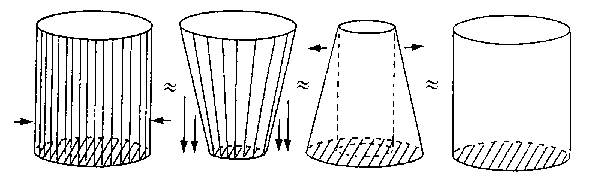
\includegraphics[width=0.5\textwidth]{figures/hom_of_pairs.pdf}
        \caption{Homeomorphism of pairs.}
        \label{fig:homeomorphism of pairs}
    \end{figure}
\end{proof}


The next Theorem shows that a map $E\to B$ that is a Serre fibration locally around each point in $B$ must be a Serre fibration. For Hurewicz fibrations the analogous statement is not generally true, i.e., a local Hurewicz fibration is not always a Hurewicz fibration, but holds, for example, over paracompact base spaces.

\begin{thm}[{{\cite[Theorem~6.3.3]{tomDieck}}}]\label{thm local fibration}
    Let $p:E\to B$ be a continuous map and $\mathcal{U}$ a collection of subsets whose interiors cover $B$. If for every $U\in\mathcal{U}$ the restriction $p_U:p^{-1}(U)\to U$ is a Serre fibration, then so is $p$.
\end{thm}
\begin{proof}
    Subdivide the cube $I^n$ into cubes of size $\delta$ and enumerate them $I_i$. We can choose $\delta$ so that each cube $I_i\times I$ is mapped inside a $U\in\mathcal{U}$ by the map $H$ that we seek to lift. This is possible by the Lebesque Lemma~\ref{Lebesque lemma}. Let $V^k\subset I^n$ denote the union of the $k$-dimensional faces of the subdivision of $I^n$.

    We have to solve the lifting problem for the space $I^n$ with initial condition $h_0$. We begin by extending $h_0$ over $I^n\times [0,\delta]$ to a lifting of $H$. We solve the lifting problems 
     \[
    \begin{tikzcd}[every matrix/.append style={name=m}]
       I^n\times\{0\} \cup V^{k-1}\times [0,\delta] \arrow[d,"i",swap]\arrow[r,"\wt{H}(k-1)"]& E\arrow[d,"p"]\\
       I^{n}\times \{0\}\cup V^k\times [0,\delta]\arrow[r,"H",swap]\arrow[ur,"\wt{H}(k)",dashed,swap] & B
    \end{tikzcd}
    \]
    for $k=0,\ldots,n$ with $V^{-1}=\varnothing$ and $\wt{H}(-1)=a$ by induction in $k$. Let $W$ be a $k$-dimensional cube and $\partial W$ the union of its $(k-1)$-dimensional faces. We can solve the lifting problems
     \[
    \begin{tikzcd}[every matrix/.append style={name=m}]
       W\times\{0\} \cup \partial W\times [0,\delta] \arrow[d,"i",swap]\arrow[r,"\wt{H}(k-1)"]& p^{-1}(U)\arrow[d,"p_U"]\\
       W\times [0,\delta]\arrow[r,"H",swap]\arrow[ur,"\wt{H}_W",dashed,swap] & U
    \end{tikzcd}
    \]
    by a map $\wt{H}_W$, since $p_U$ is a Serre fibration; here $U\in\mathcal{U}$ was chosen such that $H(W\times [0,\delta])\subset U$.

    The $\wt{H}_W$'s for different $U\in\mathcal{U}$ combine to a continuous map $\wt{H}(k):V^l\times [0,\delta]\to E$ which covers $H$ and extends $\wt{H}(k-1)$. We define $\wt{H}$ on the first layer $I^n\times [0,\delta]$ as $\wt{H}(n)$. We now treat $I^n\times [\delta,2\delta]$ similarly with initial condition given by $\restr{\wt{H}(n)}{I^n\times\{\delta\}}$ and continue in this manner inductively.
\end{proof}

\begin{prop}[{{\cite[Prop.~3.2.3]{RS2}}}]\label{prop 3.2.3 RS2}
    Serre fibrations have the \textit{lifting property} (without homotopy) w.r.t.\ all pairs of the form
    \begin{enumerate}
        \item $(K\times I,(K\times \{0\})\cup(L\times I))$, where $K$ is a $CW$-complex and $L$ is a subcomplex. This constitutes a relative \gls{hlp} for the pair $(K,L)$.
        \item $(K,L)$ where $K$ is a $CW$-complex and $L$ is a subcomplex which is a strong deformation retract of $K$.
    \end{enumerate}
\end{prop}
\begin{proof}
    Let $\pi:E\to B$ be a Serre fibration, let $K$ be a $CW$-complex and $L$ a subcomplex of $K$.

    1. Consider the lifting problem defined by some $f:K\times I\to B$ and an initial condition $\wt{f}_0:(K\times\{0\})\cup(L\times I)\to E$. We prove the assertion by induction on the dimension $k$ of the cells attached to $L$ to build $K$. The case $k=0$ is trivial. Thus, assume we have already constructed a lifting $\wt f$ over the subspace $(K^{(k)}\cup L)\times I\subset K\times I$ for some $k\geq 0$ and consider a $(k+1)$-cell $C$ not contained in $L$ with characteristic map $\chi:\bbD^{k+1}\to K$. Since $C$ is not contained in $L$, we have $C\cap (K^{(k)}\cup L)=C\cap L^{(k)}$. Hence, we wish to extend $\wt{f}$ from 
    \[(C\times\{0\}) \cup((C\cap K^{(k)})\times I)\subset C\times I\]
    to a lifting of $f$ on $C\times I$. Assume that we can extend
    \[\wt{f}\circ \restr{(\chi\times\id_I)}{(\bbD^{k+1}\times\{0\})\cup (\partial \bbD^{k+1}\times I)}\]
    to a lifting of $f\circ (\chi\times\id_I)$ on $\bbD^{k+1}\times I$. Since $\chi $ is injective on $\Int \bbD^{k+1}$, this lifting uniquely determines a lift of $f$ on $C\times I$. By Proposition~\ref{prop 3.1.11 RS2}, applied to the $CW$-complex $C\times I$, the latter is continuous.

    This argument shows that in order to prove that $\wt f$ extends to a lifting of $f$ over $(K^{(k+1)}\cup L)\times I$, it suffices to show that $\pi$ has the relative \gls{hlp} w.r.t.\ the pair $(\bbD^{k+1},\bbS^k)$. This holds by Proposition~\ref{prop 3.2.4 tomDieck} since $\pi$ is Serre fibration.

    2. Let $F:K\times I\to K$ be a strong deformation retraction from $K$ to $L$ and consider the lifting problem defined by some $f:K\to X$ and an appropriate initial condition $\wt{f}_0:L\to E$. Define $g:K\times I\to B$ by $g=f\circ F$. Since $F$ maps subsets $K\times\{1\}$ and $L\times I$ to $L$, we can also define
    \[\wt{g}_0:(K\times\{1\})\cup(L\times I)\to E,\quad \wt{g}_0(x,t)=\wt{f}_0(F(x,t)).\]
    A brief calculation shows that $\wt{g}_0$ is a lifting of $g$ over the subset $(K\times\{1\})\cup(L\times I)$. Hence, according to point 1, it can be extended to a lift $\wt{g}$ of $g$. Then, another brief calculation shows that the mapping $\wt f:K\to E$ defined by $\wt{f}(x)=\wt{g}(x,0)$ is a lifting of $f$ through $\pi$ extending $\wt{f}_0$.
\end{proof}

\begin{thm}\label{thm 6.3.1 tomDieck}
    Let $p:E\to B$ be a Serre fibration. For $B_0\subset B$ let $E_0=p^{-1}(B_0)$. Choose basepoints $*\in B_0$ and $* \in p^{-1}(*)$. Then $p$ induces for $n\geq 1$ a bijection $p_\ast:\pi_n(E,E_0,*)\to \pi_n(B,B_0,*)$.
\end{thm}
\begin{proof}
    First we show surjectivity. Let $g \in \pi_n(B,B_0,*)$ be represented by $\gamma:(\bbD^n,\bbS^{n-1},*)\to (B,B_0,*)$.
    By \gls{hlp} there exists a lifting $\wt\gamma:\bbD^n\to E$ with $\wt\gamma(*)=*$ and $p\circ \wt\gamma=\gamma$. We then have $\wt\gamma(\bbS^{n-1})\subset E_0$ and thus $\wt\gamma$ represents a preimage pf $g$ under $p_\ast$.

    To show injectivity, let $g_0,g_1\in \pi_n(E,E_0,*)$ be represented by $\gamma_0,\gamma_1$ and have the same image under $p_\ast$. Then there exists a homotopy $\phi_t:(\bbD^n,\bbS^{n-1},*)\to (B,B_0,*)$ such that $\phi_0=p\circ \gamma_0$ and $\phi_1=p\circ \gamma_1$. Consider the subspace $T=\bbD^n\times\partial I\cup *\times I$ and define $G:T\to E$ by 
    \[G(x,t)=
        \begin{cases}
            \phi_t(x),& x\in \bbD^n, t\in\{0,1\},\\
            *, & x=*, t\in I.
        \end{cases}
    \]
    The set $T\subset \partial(\bbD^n\times I)$ is transformed into $*$ if one interchanges the last two coordinates. By \gls{hlp} again, there exists a map $H:\bbD^n\times I\to E$ such that $\restr{H}{T}=G$ and $p\circ H=\phi$. We can view $H$ as a homotopy from $\gamma_0$ to $\gamma_1$.
\end{proof}
By taking $B_0$ to be a single point, we get the following corollary, which for $n\geq 2$ is just a generalization of Corollary~\ref{cor homotopy groups of coverings} for covering spaces to all fibrations.
\begin{cor}
    Given a Serre fibration $p:E\to B$ with $F=p^{-1}(*)$, there is an isomorphism of homotopy groups
    \[\pi_n(E,F,*)\cong \pi_n(B,*),\quad n\geq 1.\]
\end{cor}
With the help of this isomorphism, we immediately get a special case of the long exact sequence of a pair (Theorem~\ref{thm long exact seq of homotopy}).
\begin{thm}[Exact sequence of a Serre fibration]\label{thm long exact sequence of serre fibration}
    For a Serre fibration $p:E\to B$ with inclusion $i:F=p^{-1}(b)\subset E$ and $e\in F$ the sequence
    \begin{multline}
        \cdots \to \pi_n(F,e)\overset{i_\ast}{\to}\pi_n(E,e)\overset{p_\ast}{\to}\pi_n(B,b)\overset{\partial}{\to}\pi_{n-1}(F,e)\to\cdots\\ 
        \to \pi_0(E,e)\to \pi_0(B,b)
    \end{multline}
    is exact.
\end{thm}

The boundary map $\partial$ has the following description. Let $f:(I^n,\partial I^n)\to (B,b)$ be given. View $f$ as a map $I^{n-1}\times I\to B$ and lift it to $\wt{f}:I^n\to E$, constant and equal to $e$ on $J^{n-1}=I^{n-1}\times \{0\}\cup \partial I^{n-1}\times I$. Then $\partial[f]$ is represented by $\restr{\wt{f}}{I^{n-1}\times \{1\}}$. In plain language, a ``loop'' representing an element of $\pi_n(B)$ in the base can be lifted to a ``path'' in the total space whose ``endpoints'' lie in the same fiber $F$, and by restricting to $F$ we get a lower-dimensional ``loop'' that represents an element of $\pi_{n-1}(F)$. The very end of the sequence requires a little extra work.

\begin{defn}[Trivialization]
    Let $\pi :E\to B$ be continuous and $U\subset B$ open and contained in the image of $\pi$. A \emph{trivialization} of $\pi$ over $U$ is a homeomorphism $\varphi:\pi^{-1}(U)\to U\times F$ over $U$, i.e., a homeomorphism which satisfies $\mathrm{pr}_1\circ \varphi=\pi$ (where $\mathrm{pr}_1$ is the natural projection onto the first component of the direct product). This condition determines $F$ up to a homeomorphism since $\varphi$ induces a homeomorphism of $\pi^{-1}(u)$ with $\{u\}\times F$.
\end{defn}

\begin{defn}[Locally trivial map]
    The map $\pi$ is \emph{locally trivial} if there exists an open covering $\mathcal{U}$ of $B$ such that $\pi$ has a trivialization over each $U_\alpha\in \mathcal{U}$. 
\end{defn}

Note that a locally trivial map is open and hence a topological quotient map.

\begin{example}
    Since a product projection is a fibration, we have by Theorem~\ref{thm local fibration} that any locally trivial map is a Serre fibration.
\end{example}
\begin{example}[Exact sequence of a covering space]
    Let $p:E\to B$ be a covering map with typical fiber $F$. Since each map $\bbD^n\to F$ must be constant because of discreteness of $F$, $\pi_n(F,*)$ is trivial for $n\geq 1$. The exact sequence of $p$ then confirms the isomorphisms $\pi_n(E,f)\cong \pi_n(B,b)$, $n\geq 2$, that we proved in Corollary~\ref{cor homotopy groups of coverings}. Moreover we have the exact sequence (omitting the common basepoint)
    \[\{e\}\to \pi_1(E)\overset{p_\ast}{\to} \pi_1(B)\overset{\partial}{\to} \pi_0(F)\overset{i_\ast}{\to} \pi_0(E)\overset{p_\ast}{\to} \pi_0(B)\to \{e\}\]
    with the inclusion $i:F=p^{-1}(*)\subset E$ and $\pi_0(F)=F$. It yields for the universal covering $p:\bbR \to \bbS^1$ the familiar bijection $\partial:\pi_1(\bbS^1)\cong \bbZ$.
\end{example}

\begin{defn}[Hopf fibrations]\label{def: Hopf fibrations}
    Looking slightly ahead, consider $\bbS^{2n-1}\subset \bbC^n$ as a space with a free action of $\bbS^1=U(1)$ induced from scalar multiplication by $\rme^{2\pi\rmi  t}$. Let $U_j$ be the set of points $z=(z_1,\ldots,z_n)\in\bbC^n$ with $z_j\neq 0$. The map $z\mapsto z_j/|z_j|$ shows that $U_j\cong \bbR^{2n-1}\times \bbS^1$ is a trivial $U(1)$-space. The orbit space of this action is exactly $\mathbb{C}P^{n-1}=\bbS^{2n-1}\slash \bbS^1$. The Hopf fibration is defined as the orbit map $p:\bbS^{2n-1}\to \mathbb{C}P^{n-1}$. It is indeed a fibration because it is clearly trivial over $U_j\cap \bbS^{2n-1}$. We will also see a more explicit definition of the most important $n=2$ Hopf fibration later on.
\end{defn}

\begin{example}
    The exact sequence for the Hopf fibration, combined with $\pi_i(\bbS^1)=0$ for $i>1$ (see Corollary~\ref{cor: homotopy groups of circle}), yields the isomorphisms
    \[p_\ast: \pi_i(\bbS^{2n+1})\cong \pi_i(\mathbb{C}P^n),\; i\geq 3;\]
    and in particular $\pi_i(\bbS^3)\cong \pi_i(\bbS^2)$ for $i\geq 3$, since $\mathbb{C}P^1\cong \bbS^2$.
\end{example}

\begin{prop}[{{\cite[Prop.~6.3.8]{tomDieck}}}]\label{prop 6.3.8 tomDieck}
    Let $p:(E_1,E_0)\to B$ be a relative Serre fibration, i.e., $p:E_1\to B$ is a Serre fibration and the restriction $\restr{p}{E_0}$ is also a Serre fibration. Let $(F^1_b,F^0_b)$ be the pair of fibers over $p_1(e)=b\in B$. Then:
    \begin{enumerate}
        \item The inclusion induces bijections $\pi_n(F_b^1,F_b^0,e)\cong\pi_n(E_1,E_0,e)$.
        \item $\pi_0(E_0)\to \pi_0(E_1)$ is surjective iff $\pi_0(F_b^0)\to \pi_0(F_b^1)$ is surjective for each $b\in B$.
    \end{enumerate}
\end{prop}
\begin{proof}
    (1) We first prove the claim for $n=1$ and begin with surjectivity. Let $f:(I,\partial I,0)\to (E_1,E_0,e)$ be given. The path $\widebar{p\circ f}:I\to B$ (recall that the bar represents reversing the path) is lifted to $g:I\to E_0$ with initial point $f(1)$. Then $g(1)\in F^0_b$, and $f$ and $f\bullet g$ represent the same element in $\pi_1(E_1,E_0,e)$. The projection $p\circ(f\bullet g)$ is a nullhomotopic loop with basepoint $b$. We lift a nullhomotopy to $E_1$ with initial condition $f\bullet g$ on $I\times\{0\}$ and constant on $\partial I\times I$. The lifting is a homotopy $(I,\partial I,0)\times I\to (E_1,E_0,e)$ from $f\bullet g$ to a map into $(F^1_b,F^0_b,e)$. This proves the surjectivity.

    Suppose $f_0,f_1:(I,\partial I,0)\to (F^1_b,F^0_b,e)$ are given, and let $K:(I,\partial I,0)\times I\to (E_1,E_0,e)$ be a homotopy from $f_0$ to $f_1$. We lift $\widebar{p\circ K}$ to $L:I^2\to E_0$ with initial condition $L(s,0)=K(s,1)$ and $L(0,t)=L(1,t)=e$. The homotopy $p\circ(K\bullet_2 L)$ is a homotopy of loops which is $\rel \partial I^2$ homotopic to the constant map. We lift a homotopy to $E_1$ with initial condition $K\bullet_2 L$ on $I^2\times\{0\}$ and constant on $\partial I^2\times I$. The end is a homotopy from $f_0\bullet \kappa_e$ to $f_1\bullet\kappa_e$ (where $\kappa_e$ is a constant loop at $e$). This proves the injectivity.

    The higher dimensional case is obtained by an application to the relative Serre fibration $(\Omega^n F^1_b,\Omega^n F^0_b)\to (\Omega^n E_1,\Omega^nE_0)\to B$.

    (2) Suppose $\pi_0(E)\to \pi_0(E_1)$ is surjective. The argument above for surjectivity is used to show the surjectivity of $\pi_0(F^0_b)\to \pi_0(F^1_b)$. The opposite implication is easy.
\end{proof}





\section{Higher connectivity}

For many applications it is important to know that the homotopy groups of a space vanish in a certain range. We discuss several reformulations of this fact. In the following $\pi_0(X,x_0)=\pi_0(X)$. The space $\bbD^0$ is a singleton and $\bbS^{-1}=\varnothing$.

\begin{prop}[{{\cite[Prop.~6.7.1]{tomDieck}}}]\label{prop 6.7.1 tomDieck} 
Let $n\geq 0$. \gls{tfae}:
\begin{enumerate}
    \item $\pi_n(X,x)=0$ for each $x\in X$.
    \item Each map $\bbS^n\to X$ has an extension to $\bbD^{n+1}$.
    \item Each map $\partial \bbD^{n+1}\to X$ has an extension to $\bbD^{n+1}$.
\end{enumerate}
\end{prop}
\begin{proof}
    The case $n=0$ is trivial. The equivalence of (2) and (3) is a consequence of the homeomorphism $(\bbD^{n+1},\bbS^n)\cong(I^{n+1},\partial I^{n+1})$. Suppose $f:\bbS^n\to X$ is given. Use $e_1=(1,0,\ldots)\in \bbS^n$ as a base point and think of $f$ as representing an element of $\pi_n(X,x)$. If (1) holds, then $f$ is pointed null homotopic. A null homotopy $\bbS^n\times I\to X$ factors over the quotient map $\bbS^n\times I\to \bbD^{n+1}$, $(x,t)\mapsto (1-t)e_1+tx$ and yields an extension of $f$. Conversely, let an element $\alpha$ of $\pi_n(X,x)$ be represented by a pointed map $f:(\bbS^n,e_1)\to (X,x)$. If this map has an extension $F$ to $\bbD^{n+1}$, then $(F,f)$ represents $\beta\in \pi_n(X,X,x)=0$ with $\partial\beta=\alpha$.
\end{proof}

\begin{prop}[{{\cite[Prop.~6.7.3]{tomDieck}}}]\label{prop 6.7.3 tomDieck}
    Let $n\geq 1$. The following assertions about a topological pair $(X,A)$ are equivalent:
    \begin{enumerate}[label=(\arabic*)]
        \item $\pi_n(X,A,*)=0$ for each choice of $*\in A$.
        \item Each map $f:(I^n,\partial I^n)\to (X,A)$ is as a map of pairs homotopic to a constant map.
        \item Each map $f:(I^n,\partial I^n)\to (X,A)$ is homotopic $\rel \partial I^n$ to a map into $A$.
    \end{enumerate}
\end{prop}
\begin{proof}
    $(1)\implies(2)$. Let $f:(I^n,\partial I^n)\to (X,A)$ be given. Since $J^{n-1}$ is contractible, there exists a homotopy of the restriction $f:J^{n-1}\to A$ to a constant map. Since $J^{n-1}\subset \partial I^n$ and $\partial I^n\subset I^n$ are cofibrations, $f$ is as a map of pairs homotopic to $g:(I^n,\partial I^n)\to (X,A)$ such that $g(J^{n-1})=\{a_0\}$. Since $\pi_n(X,A,a_0)=0$, the map $g:(I^n,\partial I^n,J^{n-1})\to (X,A,a_0)$ is nullhomotopic as a map of triples.

    $(2)\implies(3)$ by the compression criterion (Proposition~\ref{prop: compression criterion}).

    $(3)\implies (1)$. Let $f:(I^n,\partial I^n,J^{n-1})\to (X,A,*)$ be given. By assumption (3), $[f]$ is contained in the image of $\pi_n(A,A,*)\to \pi_n(X,A,*)$. Now use $\pi_n(A,A,*)=0$.
\end{proof}



\begin{defn}[$n$-compressible pair]\index{$n$-compressible space}
    A topological pair $(X,A)$ is called $n$-compressible if (1)-(3) in Proposition~\ref{prop 6.7.3 tomDieck} hold. More generally, we call a map $f:X\to Y$ $n$-compressible if for each commutative diagram 
    \[
    \begin{tikzcd}[every matrix/.append style={name=m}, row sep=large, column sep=large]
       \partial \bbS^{n-1} \arrow[r,"\varphi"]\arrow[d,"i",swap] & X\arrow[d,"f"]\\
       \bbD^n \arrow[r,"\varPhi", swap]\arrow[ur,"\varPsi",dashed,swap] & Y
    \end{tikzcd}
    \]
    there exists $\varPsi:\bbD^n\to X$ such that $\restr{\varPsi}{\partial \bbD^n}=\varphi$ and $f\circ \varPsi\simeq \varPhi$ $\rel \partial \bbD^n$ (this amounts to (3) of Proposition~\ref{prop 6.7.3 tomDieck}). This notion is invariant under compositions with homotopy equivalences of the target space $Y$.
\end{defn}

\begin{prop}[{{\cite[Prop.~6.7.5]{tomDieck}}}]\label{prop 6.7.5 tomDieck}
    Let $n\geq 0$. The following assertions about a pair $(X,A)$ are equivalent:
    \begin{enumerate}
        \item Each map $f:(\bbD^q,\partial \bbD^q)\to (X,A)$, $q\in (0,\ldots,n)$ is $\rel \partial \bbD^q$ homotopic to a map into $A$.
        \item The inclusion $j:A\hookrightarrow X$ induces for each basepoint $a\in A$ a bijection $j_\ast:\pi_q(A,a)\to \pi_q(X,a)$ for $q<n$ and a surjection for $q=n$.
        \item $\pi_q(X,A,a)=0$ for $q=1,\ldots,n$ and each $a\in A$, and $\pi_0(A)\to \pi_0(X)$ is surjective.
    \end{enumerate}
\end{prop}
\begin{proof}
    $(1)\Leftrightarrow (3)$. The surjectivity of $\pi_0(A)\to \pi_0(X)$ is equivalent to (1) for $q=0$. The other cases follow from Proposition~\ref{prop 6.7.3 tomDieck}.

    $(2)\Leftrightarrow(3)$ follows from the exact sequence of the pair (Theorem~\ref{thm long exact seq of homotopy}).
\end{proof}


\begin{defn}[$n$-connected pair]\index{$n$-connected pair}
    A topological pair $(X,A)$ is called $n$-connected if (1)-(3) in Proposition~\ref{prop 6.7.5 tomDieck} hold. We call $(X,A)$ $\infty$-connected if the pair is $n$-connected for each $n$. A pair is $\infty$-connected iff $j_\ast:\pi_n(A,a)\to \pi_n(X,a)$ is always bijective. If $X\neq\varnothing$ but $A=\varnothing$ we say that $(X,A)$ is $(-1)$-connected, and $(\varnothing,\varnothing)$ is $\infty$-connected.
\end{defn}

\begin{defn}[Cone]\index{Cone}
    Given a space $X$, its cone $CX$ is defined as result of attaching the cylinder $X\times [0,1]$ by its face $X\times\{0\}$ to a point $*$ along the projection $p:X\times \{0\}\to *$.
\end{defn}


\begin{prop}[{{\cite[Prop.~6.7.6]{tomDieck}}}]\label{prop 6.7.6 tomDieck}
    Let $n\geq 0$. The following assertions about a space $X$ are equivalent:
    \begin{enumerate}
        \item $\pi_q(X,x)=0$ for $0\leq q\leq n$ and $x\in X$.
        \item The pair $(CX,X)$ is $(n+1)$-connected.
        \item Each map $f:\partial I^q\to X$, $0\leq q\leq n+1$ has an extension to $I^q$.
    \end{enumerate}
\end{prop}
\begin{proof}
    The cone $CX$ is contractible, therefore $\partial:\pi_{q+1}(CX,X,*)\cong \pi_q(X,*)$. This and Proposition~\ref{prop 6.7.5 tomDieck} shows the equivalence of (1) and (2). The equivalence of (1) and (3) is based on Proposition~\ref{prop 6.7.1 tomDieck}.
\end{proof}

\begin{defn}[$n$-connected space]\index{$n$-connected space}
    A space $X$ is called $n$-connected if (1)-(3) in Proposition~\ref{prop 6.7.6 tomDieck} hold. Note that this is compatible with previous definitions for $n=0$ (path-connected) and $n=1$ (simply-connected).
\end{defn}

\begin{defn}[$n$-equivalence]\index{$n$-equivalence}\index{Weak equivalence}
    Let $f:X\to Y$ be a map and $X\subset Z_f$ the inclusion into the mapping cylinder (recall the definition in Figure~\ref{fig:mapping cyl}). Then $f$ is said to be $n$-connected if $(Z_f,X)$ is $n$-connected. We then also say that $f$ is an $n$-equivalence. Thus $f$ is $n$-connected iff $f_\ast:\pi_q(X,x)\to \pi_q(Y,f(x))$ is for each $x\in X$ bijective for $q<n$ and surjective for $q=n$. If $f$ is an $\infty$-equivalence we also call it a weak (homotopy) equivalence, which happens iff $f_\ast$ is bijective for all $x\in X$ in all degrees.
\end{defn}

\begin{prop}[{{\cite[Prop.~6.7.7]{tomDieck}}}]\label{prop 6.7.7 tomDieck}
    Let $p:(E_1,E_0)\to B$ be a relative Serre fibration (see Proposition~\ref{prop 6.3.8 tomDieck}). Let $(F^1_b,F^0_b)$ be the pair of fibers over $b\in B$. Then the pair $(E_1,E_0)$ is $n$-connected iff the pairs $(F^1_b,F^0_b)$ are $n$-connected for all $b\in B$.
\end{prop}
\begin{proof}
    This is a direct consequence of Proposition~\ref{prop 6.3.8 tomDieck}.
\end{proof}

\begin{thm}[{{\cite[Theorem~6.7.9]{tomDieck}}}]\label{thm 6.7.9 tomDieck}
    Let $\varphi:(X,X_0,X_1)\to (Y,Y_0,Y_1)$ be a map such that the restrictions $\varphi_i:X_i\to Y_i$ are $n$-connected and $\varphi_{01}:X_0\cap X_1\to Y_0\cap Y_1$ is $(n-1)$-connected. Suppose $X=X_0^\circ \cup X_1^\circ$ and $Y=Y_0^\circ \cup Y_1^\circ$ where $\ ^\circ$ denotes interiors. Then $\varphi $ is an $n$-equivalence.
\end{thm}

\begin{cor}[{{\cite[Prop.~6.7.10]{tomDieck}}}]\label{prop 6.7.10 tomDieck}
    Let $f:X\to Y$ be an $n$-connected map between spaces with nondegenerate basepoints. Then the suspension $\Sigma f:\Sigma X\to \Sigma Y$ is $(n+1)$-connected. If $X$ is $n$-connected, then $\Sigma X$ is $(n+1)$-connected. The sphere $\bbS^{k+1}$ is $k$-connected.
\end{cor}
\begin{proof}
    Let $\Sigma 'X$ denote the unpointed suspension of $X$. This is a quotient of $X\times I$ and covered by the open cones $C_0=X\times [0,1)\slash X\times\{0\}$ and $C_1=X\times (0,1]\slash X\times\{1\}$ with intersection $X\times (0,1)$. We can apply Proposition~\ref{prop 6.7.7 tomDieck} directly; the cones are contractible and therefore the induced maps $C_j(X)\to C_j(Y)$ are $\infty$-connected. In the case of a space $X$ with a nondegenerate basepoint the quotient map $\Sigma 'X\to \Sigma X$ is a homotopy equivalence.
\end{proof}

\begin{thm}[{{\cite[Theorem~6.7.11]{tomDieck}}}]\label{thm 6.7.11 tomDieck}
    Let $f:X\to Y$ be a continuous map. Let $\{U_j\}_j$ and $\{V_j\}_j$ be open coverings of $X$ and $Y$ such that $f(U_j)\subset V_j$. Suppose that for each finite subset of indices the induced map $f_J:\bigcap_{j\in J}U_j\to \bigcap_{j\in J}V_j$ is a weak equivalence. Then $f$ is a weak equivalence.
\end{thm}
\begin{proof}
    By passage to the mapping cylinder we can assume that $f$ is an inclusion. Let $h:(I^n,\partial I^n)\to (Y,X)$ be given. We have to deform $h$ $\rel \partial I^n$ into $X$. By compactness of $I^n$ is suffices to work with finite coverings. A simple induction reduces the problem to a covering by only two sets $j=0,1$. Then we apply Theorem~\ref{thm 6.7.9 tomDieck}.
\end{proof}






\section{Excision for homotopy groups}

The following fundamental theorem, which we provide without proof, is an advanced relative of the Seifert-van~Kampen Theorem~\ref{thm seifert-van kampen}. While the latter allowed us to compute fundamental groups of ``composite'' spaces as free products of simpler pieces, this theorem indicates that a similar procedure for higher homotopy groups does not exist. In fact, the best case scenario is that if the pieces are sufficiently connected in low dimensions, then the composite space will inherit the homotopy groups up to some dimension. This is why it is commonly said that ``excision fails in homotopy'', unlike in homology.

\begin{thm}[Blakers-Massey excision theorem {{\cite[Thm~6.4.1]{tomDieck}}}]
    Let $X=U_0\cup U_1$ be covered by two open subspaces $U_0$ and $Y_1$ with non-empty intersection $V=U_0\cap U_1$. Suppose that $(U_0,V)$ is $p$-connected and $(U_1,V)$ is $q$-connected, i.e.
    \[
    \begin{matrix}
        \pi_i(U_0,V,*)=0,\quad 1\leq i\leq p,\; p\geq 0,\\
        \pi_i(U_1,V,*)=0,\quad 1\leq i\leq q,\; q\geq 0
    \end{matrix}
    \]
    for each basepoint $*\in V$. Then the \emph{excision map}, induced by the inclusion,
    \[i_\ast : \pi_n(U_1,V,*)\to \pi_n(X,U_0,*)\]
    is an isomorphism for $1\leq n <p+q$ and surjective for $n=p+q$ (for each $*\in X)$. In the case $p=0$, there is no condition on $\pi_i(U_0,V,*)$.
\end{thm}

\begin{cor}[{{\cite[Prop.~6.4.2]{tomDieck}}}]\label{prop 6.4.2 tomDieck}
    If in the above $(U_1,V)$ is $q$-connected then $(X,U_0)$ is $q$-connected.
\end{cor}
\begin{proof}
    This is a special case of the excision theorem which also directly follows from Theorem~\ref{thm 6.7.9 tomDieck}.
\end{proof}

For the sphere $\bbS^n$, introduce the following hemispheres and punctured spheres
\[\bbD^n_\pm=\{x\in \bbS^n\subset \bbR^{n+1}\mid \pm x_{n+1}\geq 0\}\subset H^n_\pm=\{x\in \bbS^n\mid x\neq \pm e_{n+1}\}.\]
We use the equatorial point $*=-e_1$ as a basepoint.

\begin{lem}[{{\cite[Lemma~6.4.3]{tomDieck}}}]\label{lem 6.4.3 tomDieck}
   There are isomorphisms $\partial:\pi_{i+1}(D_-^{n+1},\bbS^n,*)\to \pi_i(\bbS^n,*)$ for $i\geq 0$, $n\geq 0$ and $\pi_i(\bbS^n,*)\to \pi_i(\bbS^n,D_\pm^n,*)$ for $i\geq 0$, $n\geq 1$.
\end{lem}
\begin{proof}
    In the first case we use the exact sequence of the pair $(\bbD^{n+1}_-,\bbS^n)$. The space $\bbD^{n+1}_-$ is contractible and hence $\pi_i(\bbD^{n+1}_-,*)=0$ for $i\geq 0$ and $n\geq 0$.

    In the second case we consider similarly the exact sequence of $(\bbS^n,\bbD^n_\pm)$. Note that $*=-e_1\in D_\pm^n$ for $n\geq 1$.
\end{proof}

Thus for $n\geq 0$ we have a diagram with the isomorphisms 
\[
    \begin{tikzcd}[every matrix/.append style={name=m}, row sep=large, column sep=large]
       \pi_i(\bbS^n,*) \arrow[r,"E"] & \pi_{i+1}(\bbS^{n+1},*)\arrow[d,"\cong"]\\
       \pi_{i+1}(\bbD^{n+1}_-,\bbS^n,*)\arrow[u,"\overset{\partial}{\cong}",swap] \arrow[r,"i_\ast", swap] & \pi_{i+1}(\bbS^{n+1},D_+^{n+1},*).
    \end{tikzcd}\label{3795}
\]
The morphism $i_\ast$ is induced by the inclusion and $E$ is defined so as to make the diagram commutative. Note that the inductive proof of item 1 in the next theorem uses only Corollary~\ref{prop 6.4.2 tomDieck}.

\begin{thm}[{{\cite[Thm~6.4.4]{tomDieck}}}]\label{thm 6.4.4 tomDieck}
    \begin{enumerate}
        \item $\pi_i(\bbS^n)=0$ for $i<n$ (recall that we already showed this in Corollary~\ref{cor pi_n(S^k)=0}).
        \item The homomorphism $i_\ast$ in diagram \eqref{3795} is an isomorphism for $i\leq 2n-2$ and an epimorphism for $i=2n-1$. A similar statement holds for $E$.
    \end{enumerate}
\end{thm}
\begin{proof}
    Let $N(n)$ be the statement (1) and $E(n)$ be the statement (2). Obviously $N(1)$ holds. Assume $N(n)$ holds. We then deduce $E(n)$. We apply the excision theorem to $(X,U_0,U_1,V)=(\bbS^{n+1},D_+^{n+1},D_-^{n+1},\bbS^n)$. By $N(n)$ and Lemma~\ref{lem 6.4.3 tomDieck} we have $\pi_i(\bbS^n)\cong \pi_{i+1}(D_\pm^{n+1},\bbS^n)=0$ for $0\leq i <n$. We use the excision theorem for $p=q=n$ and see that $i_\ast$ is surjective for $i+1\leq 2n$ and bijective for $i+1\leq 2n-1$. Finally, $E(n)$ and $N(n)$ imply $N(n+1)$.

    In order to have the correct hypotheses for the excision theorem, we thicken the spaces, replace $D_\pm^n$ by $H^n_\pm$ and note that the inclusions $D_\pm^n\subset H^n_\pm$ and $\bbS^{n-1}\subset H^n_+\cap H^n_-$ are homotopy equivalences.
\end{proof}
\begin{cor}[{{\cite[Prop.~5.11]{Bredon}}}] 
    The pair $(\bbD^{n+1},\bbS^n)$ is $n$-connected.
\end{cor}
\begin{proof}
    This follows from the exact sequence $\pi_r(\bbD^{n+1})\to \pi_r(\bbD^{n+1},\bbS^n)\to \pi_{r-1}(\bbS^n)$ for $r\leq n$, where the two groups on the sides vanish.
\end{proof}


\begin{prop}[{{\cite[Prop.~6.4.5]{tomDieck}}}]\label{prop 6.4.5 tomDieck}
    The homomorphism $\pi_i(\bbD^{n+1},\bbS^n,*)\to \pi_i(\bbD^{n+1}\slash \bbS^n,*)$ induced by the quotient map is an isomorphism for $i\leq 2n-1$ and an epimorphism for $i=2n$.
\end{prop}
\begin{proof}
    Consider the commutative diagram
    \[
    \begin{tikzcd}[every matrix/.append style={name=m}, row sep=large, column sep=large]
       \pi_i(D_-^{n+1},\bbS^n,*) \arrow[r]\arrow[d,"i_\ast",swap] & \pi_i(D_-^{n+1}\slash \bbS^n,*) \arrow[d,"(1)"]\\
       \pi_{i+1}(\bbS^{n+1},\bbD^{n+1}_+,*)\arrow[r,"(2)",swap] & \pi_{i}(\bbS^{n+1}\slash D_+^{n+1},*).
    \end{tikzcd}
    \]
    The map (1) is induced by a homeomorphism and the map (2) by a homotopy equivalence, hence both are isomorphisms. Now apply Theorem~\ref{thm 6.4.4 tomDieck}.
\end{proof}

The homomorphism $E$ is essentially the suspension homomorphism:
\[\Sigma_\ast: \pi_n(X)\underset{\cong}{\overset{\partial}{\leftarrow}}\pi_{n+1}(CX,X)\overset{q_\ast}{\to}\pi_{n+1}(CX\slash X)=\pi_{n+1}(\Sigma X)\]
with the quotient map $q:\bbD^{n+1}\to \bbS^{n+1}=\bbD^{n+1}\slash \bbS^n$. The next result is the famous suspension theorem of Freudenthal.

\begin{thm}[Freudenthal's suspension theorem {{\cite[Theorem~6.4.6]{tomDieck}}}]\label{thm 6.4.6 tomDieck freudenthal}
    The suspension $\Sigma_\ast:\pi_i(\bbS^n)\to \pi_{i+1}(\bbS^{n+1})$ is an isomorphism for $i\leq 2n-2$ and an epimorphism for $i=2n-1$.
\end{thm}
\begin{proof}
    We have to show that $q_\ast:\pi_{i+1}(CX,X)\to \pi_{i+1}(CX\slash X)$ is for $X=\bbS^n$ an isomorphism (epimorphism) in the appropriate range. This follows from Proposition~\ref{prop 6.4.5 tomDieck}; one has to use that  $\bbD^{n+1}_-$ is the (pointed) cone on $\bbS^n$.
\end{proof}

\begin{thm}[{{\cite[Theorem~6.4.7]{tomDieck}}}]\label{thm 6.4.7 tomDieck freudenthal}
    $\pi_n(\bbS^n)\cong \bbZ$ and $\Sigma_\ast:\pi_n(\bbS^n)\to \pi_{n+1}(\bbS^{n+1})$ is an isomorphism ($n\geq 1$). The group $\pi_n(\bbS^n)$ is generated by the identity map of $\bbS^n$.
\end{thm}
\begin{proof}
    From the exact sequence of the Hopf fibration $\pi_2(\bbS^3)\to \pi_2(\bbS^2)\to \pi_1(\bbS^1)\to \pi_1(\bbS^3)$ and $\pi_j(\bbS^3)=0$ for $j=1,2$, we obtain an isomorphism $\partial:\pi_2(\bbS^2)\to \pi_1(\bbS^1)\cong \bbZ$. From Theorem~\ref{thm 6.4.6 tomDieck freudenthal} we obtain a surjection $\Sigma_\ast:\pi_1(\bbS^1)\to \pi_2(\bbS^2)$; this is an isomorphism, since both groups are isomorphic to $\bbZ$. For $n\geq 2$, Theorem~\ref{thm 6.4.6 tomDieck freudenthal} directly gives an isomorphism $\Sigma_\ast$. We know that $\pi_1(\bbS^1)$ is generated by the identity map, and $\Sigma_\ast$ respects the identity.
\end{proof}

This proof clearly extends to two cones over any space $X$, so by using the adjunction $[\Sigma X,Y]\cong[X,\Omega Y]$ we get the more general form of this Theorem.

\begin{thm}[Freudenthal's suspension theorem {{\cite[Thm.~6.4.6]{tomDieck}}}]\index{Theorem!Freudenthal's suspension}
Let $X$ be an $n$-connected space, i.e., $\pi_i(X)=0$ for $0\leq i\leq n$. Then the homomorphism $\pi_k(X)\to \pi_k(\Omega \Sigma X)$ induced by the inclusion $X\hookrightarrow \Omega\Sigma X$ is an isomorphism for $k\leq 2n-2$ and an epimorphism for $k=2n-1$.

Furthermore, since $\pi_{k+1}(\Sigma X)\cong[\bbS^{k+1};\Sigma X]\cong[\bbS^k;\Omega \Sigma X]\cong\pi_k(\Omega \Sigma X)$, for $k\leq 2n-2$ there is an isomorphism $\pi_k(X)\cong \pi_{k+1}(\Sigma X)$.
\end{thm}

Since $\id_{\bbS^n}$ generates the $n$-th homotopy group of $\bbS^n$, this allows us to make the following definition.

\begin{defn}[Degree on spheres]\index{Degree}
    For a map $f:\bbS^n\to \bbS^n$, its degree $\deg f$ is the integer such that $[f]=[\mathrm{id}_{\bbS^n}]^{\deg f}$ in $\pi_n(\bbS^n)$.
\end{defn}

\begin{example}[Hopf fibrations]\label{example Hopf pi3(S2)}
    We continue the discussion of the Hopf fibrations \ref{def: Hopf fibrations}. The Hopf fibration $\bbS^{2n+1}\to \mathbb{C}P^n$ and $\pi_i(\bbS^{2n+1})=0$ for $i\leq 2n$ yield $\pi_2(\mathbb{C}P^n)\cong \pi_1(\bbS^1)\cong \bbZ$ and $\pi_i(\mathbb{C}P^n)=0$ for $0\leq i \leq 2n$, $i\neq 2$. The inclusion $\bbS^{2n+1}\to \bbS^{2n+3}$, $z\mapsto (z,0)$ induces an embedding $\mathbb{C}P^n\subset \mathbb{C}P^{n+1}$. We compare the corresponding Hopf fibrations and their exact sequences and conclude $\pi_2(\mathbb{C}P^n)\cong \pi_2(\mathbb{C}P^{n+1})$. Let $\mathbb{C}P^\infty =\bigcup_{n\geq 1}\mathbb{C}P^n$ be the colimit (the topology on it is defined as the finest topology under which all inclusions $\mathbb{C}P^n\hookrightarrow \mathbb{C}P^\infty$ are continuous). The inclusions induce $\pi_i(\mathbb{C}P^n)\cong\pi_i(\mathbb{C}P^\infty)$ for $i\leq 2n$. A proof uses the fact that a compact subset of $\mathbb{C}P^\infty$ is contained in some finite $\mathbb{C}P^N$. Therefore $\mathbb{C}P^\infty$ is a space with a single nontrivial homotopy group $\pi_2(\mathbb{C}P^\infty)\cong\bbZ$.

    Particularly notable is the special case 
    \[\pi_3(\bbS^2)\cong \pi_3(\bbS^3)\cong\bbZ.\]
    This is the first of the ``nontrivial'' homotopy groups of spheres $\pi_k(\bbS^n), k>n$, and the only one that can be computed without much more advanced homology theory.

    We have the similar results for real projective spaces. The double coverings $\bbS^n\to \RP^n$ are used to show that $\pi_1(\RP^2)\cong \pi_1(\RP^3)\cong\cdots =\cong \pi_1(\RP^\infty)\cong \bbZ_2$, induced by the inclusions $\RP^n\hookrightarrow\RP^{n+1}$ for $i<n$ and $\pi_i(\RP^n)=0$ for $0\leq i< n$, $i\neq 1$. The space $\RP^\infty$ therefore has a single nontrivial homotopy group $\pi_1(\RP^\infty)\cong\bbZ_2$.
\end{example}


\begin{example}[Lens spaces]\index{Lens spaces}
    Recall the lens space $L=L_m(l_1,\ldots,l_n)$ from Example~\ref{example Lens spaces}. It can be given a structure of a $CW$-complex with one cell in each dimension from $0$ to $2n-1$ so that the degree of the attaching maps alternates between $0$ and $m$ (starting with degree $0$ for the map $\partial \bbD^1\to L^{(0)}$).
\end{example}


\begin{example}[$\pi_3(\bbS^2\vee \bbS^2)\cong \bbZ^3$]
    Let us compute $\pi_3(\bbS^2\vee \bbS^2)$. We have an inclusion $i: \bbS^2\vee \bbS^2\hookrightarrow \bbS^2\times \bbS^2$, because $\bbS^2\times \bbS^2$ can be realized as a $CW$-complex that differs from $\bbS^2\vee \bbS^2$ only by an addition of a 4-cell. Observe that the induced homomorphism on the homotopy groups is surjective:
    \[i_\ast: \quad \pi_n(\bbS^2\vee \bbS^2)\to \pi_n(\bbS^2\times \bbS^2)=\pi_n(\bbS^2)\oplus \pi_n(\bbS^2).\]
    (Here we used the fact that a smash product with $\bbS^k$ is homeomorphic to the iterated reduced suspension $\Sigma^k$, and $\Sigma^k \bbS^n=\cong \bbS^{n+k}$.) This allows us to insert extra zeroes into the long exact sequence for the pair $(\bbS^2\times \bbS^2,\bbS^2\vee \bbS^2)$ without breaking its exactness, which splits it into the short exact sequences
    \[0\to \pi_{n+1}(\bbS^2\times \bbS^2,\bbS^2\vee \bbS^2)\to \pi_n(\bbS^2\vee \bbS^2)\overset{i_\ast}{\to} \pi_n(\bbS^2\times \bbS^2)\to 0.\]
    For $n=3$, since $\bbS^2\vee \bbS^2$ is 1-connected and the remaining 4-cell is 4-connected, we can use the excision theorem to compute
    \[\pi_4(\bbS^2\times \bbS^2,\bbS^2\vee \bbS^2)\cong \pi_4(\bbS^2\times \bbS^2\slash \bbS^2\vee \bbS^2)\cong \pi_4(\bbS^2\wedge \bbS^2) \cong\pi_4(\bbS^4)\cong \bbZ.\]
    At the same time, $\pi_3(\bbS^2\times \bbS^2)=\pi_3(\bbS^2)\oplus \pi_3(\bbS^2)=\bbZ^2$ (generated by the Hopf fibrations from the preceding Example~\ref{example Hopf pi3(S2)}). Thus we have the exact sequence
    \[0\to \bbZ\to \pi_3(\bbS^2\vee \bbS^2)\to \bbZ^2\to 0,\]
    which implies $\pi_3(\bbS^2\vee \bbS^2)=\bbZ^3$ because every short exact sequence of the form $0\to A\overset{i}{\to} B\overset{p}{\to} \bbZ^2\to 0$ splits (the splitting monomorphism $j:\bbZ^2\to B$ can be constructed by defining it on the basis $j(1,0)=b_1$ and $j(0,1)=b_2$, where $b_1,b_2\in B$ are any two elements such that $p(b_1)=(1,0)$ and $p(b_2)=(0,1)$; it is then easy to check that $p\circ j=\id_{\bbZ^2}$ and hence $B\cong A\oplus \bbZ^2$).

    This construction is a special case of the \emph{Whitehead product}\index{Whitehead product} $\pi_k(X)\times\pi_l(X)\to \pi_{k+l-1}(X)$. Given $f:\bbS^k\to X$ and $g:\bbS^l\to X$, their Whitehead product is the homotopy class denoted
    \[[f,g]\in \pi_{k+l-1}(X)\]
    and represented by the composition 
    \[\bbS^{k+l-1}\overset{\chi}{\to} \bbS^k\vee \bbS^l\overset{f\vee g}{\to} X,\]
    where $\chi$ is the attaching map for the single $(k+l)$-cell in the $CW$-complex $\bbS^k\times \bbS^l$ which consists of $\bbS^k\vee \bbS^l$ and that cell ($\chi$ maps the boundary of the $(k+l)$-disk to the $(k+l-1)$-skeleton, which in this case is $\bbS^k\vee \bbS^l$). In the case above, the third ``unexpected'' generator of $\pi_3(\bbS^2\vee \bbS^2)$ is $[i_1,i_2]$, where $i_1,i_2:\bbS^2\to \bbS^2\vee \bbS^2$ are the inclusion maps for the two 2-spheres. 
    
    Another simple Whitehead product is $[\id_{\bbS^2},\id_{\bbS^2}]\in\pi_3(\bbS^2)$. It is represented by the map obtained by gluing $\bbS^2\vee \bbS^2\subset \bbS^3$ onto $\bbS^2$. Since we already know that $\pi_3(\bbS^2)$ is generated by the Hopf fibration $p_{\mathrm{Hopf}}$ and this map clearly has winding number $2$, we find that 
    \[[\id_{\bbS^2},\id_{\bbS^2}]=2[p_{\mathrm{Hopf}}]\]
    (although there might also be a minus sign depending on how one defines the Hopf fibration).
\end{example}

\begin{xca}[{{\cite[Thm.~6.10.5]{tomDieck}}}]
    Let $X$ and $Y$ be well-pointed (i.e., with non-degenerate basepoints) and assume that $\pi_i(X)=\pi_j(Y)=0$ for $i<p,j<q$ with $p,q\geq 2$. Show that the inclusion $X\vee Y\hookrightarrow X\times Y$ induces an isomorphism of the $\pi_i$-groups for $i\leq p+q-2$. Also show that $\pi_i(X\times Y,X\vee Y)$ and $\pi_i(X\wedge Y)$ vanish for $i\leq p+q-1$.
\end{xca}

\begin{xca}[{{\cite[Exercise 6.11]{tomDieck}}}]
    Extend the above example to determine $\pi_{2n-1}(\bbS^n\vee \bbS^n)$ for $n\geq 2$.
\end{xca}


\clearpage 

\chapter{Lie Theory I: Basics}\label{ch Lie I}

\section{Lie groups}

\begin{defn}[Topological group]\index{Topological group}
    A topological group is a group $G$ together with a topology on it that is compatible with the group structure. That is, both the inversion $g\mapsto g^{-1}$ and the multiplication $(g,h)\mapsto gh$ maps are continuous. This is equivalent to requiring that the map $G\times G\to G$ given by $(g,h)\mapsto gh^{-1}$ is continuous.
\end{defn}

Topological groups form a very big class and include things like ``infinite-dimensional Lie groups'', $p$-adic numbers, rational numbers, etc. It turns out that every locally compact and locally contractible topological group (in particular topological groups that are also topological manifolds) have a unique smooth structure compatible with the group structure, which is what a Lie group is. Hence we skip right to the definition of Lie groups, and for the most part will assume that they are smooth.

\begin{defn}[Lie group]\index{Lie group}
    A (real) Lie group is a group $G$ with a structure of a differentiable (or $C^k$-differentiable, $C^\infty$-smooth, $C^\omega$-analytic) manifold on it that is compatible with the group structure. That is, the map $G\times G\to G$ given by $(g,h)\mapsto gh^{-1}$ is differentiable (resp.~$C^k$, $C^\infty$, $C^\omega$). A complex Lie group is defined similarly, with both the manifold structure and the group structure being holomorphic (complex analytic).
\end{defn}

We will show that any twice differentiable Lie group has a unique compatible real analytic structure. In fact, one can show that differentiability is not required at all, and any topological manifold with a continuous group structure has a unique structure of an analytic Lie group. This is why most authors assume that Lie groups are smooth by definition.

\begin{prop}[{{\cite[Thm.~1.6.3]{DK}}}]
    Any twice-differentiable Lie group $G$ has a unique structure of a real analytic manifold which turns it into a real analytic Lie group, and such that the identity map on $G$ is a $C^2$-diffeomorphism between the two structures.
\end{prop}


\begin{defn}[Group translation and adjoint operators]\index{Translation operator}\index{Adjoint operator}
    The left and right translation operators on a group $G$ are defined by
    \[\rmL_g(h)=gh,\quad \rmR_g(h)=hg,\quad \text{for}\; g,h\in G.\]
    The group adjoint, or \emph{conjugation}, operator corresponding to an element $g\in G$ is the map
    \[\Adg_g:G\to G,\quad \Adg_g h=\rmL_g\circ \rmR_g^{-1}(h)=ghg^{-1}.\]
\end{defn}


\begin{example}[Lie groups]
    \begin{enumerate}[label=(\alph*)]
        \item Let $\bbK=\bbR ,\mathbb{C}$, or $\bbH $ (quaternions, see below). Every $\bbK$-vector space $V$ is a Lie group w.r.t.\ its additive structure and the manifold structure of the real vector space obtained from $V$ by restriction of the algebraic structure. The dimension is $\dim_{\bbR }\bbK\cdot \dim V$.
        \item Every finite or countable group with discrete topology is a Lie group.
        \item The direct product $G\times H$ of two Lie groups $G,H$ is a Lie group with the product group structure and the differentiable structure of the product of manifolds.
        \item $\GL_n(\bbR )$ is the set of invertible $n\times n$ matrices with real entries. It is a group under matrix multiplication and an open subset of $\Mat_n(\bbR )\cong \bbR^{n^2}$ (cf.\ Example~\ref{example smooth maps} for the smoothness of its operations). Matrix multiplication is obviously smooth and inversion is smooth by Cramer's rule.
        \item $\GL^+_n(\bbR )$, which is the subset of $\GL_n(\bbR )$ consisting of matrices with positive determinant. It is still a group and an open subset of $\GL_n(\bbR )$.
        \item If $H\subset G$ is an open subgroup (a subgroup that is an open subset) of a Lie group $G$, then $H$ is a Lie group with the inherited group and manifold structures.
        \item For any real or complex finite-dimensional vector space $V$, the group $\GL(V)$ of endomorphisms of $V$ is a Lie group.
        \item The unit circle $\bbS^1\subset \mathbb{C}^\ast$ with multiplication inherited from $\mathbb{C}$ is a Lie group.
        \item The $n$-torus $\bbT^n=\bbS^1\times\cdots\times \bbS^1$ is an $n$-dimensional abelian Lie group.
    \end{enumerate}
\end{example}

\begin{defn}[Lie group homomorphism]\index{Homomorphism!of Lie groups}
    A Lie group homomorphism between two Lie groups $G,H$ is a smooth map $F:G\to H$ that is also a group homomorphism. If it is a diffeomorphism, it is called an isomorphism. These maps comprise the morphisms of the category $\mathsf{LieGr}$ of Lie groups.
\end{defn} 

\begin{example}[Lie group morphisms]
    \begin{enumerate}[label=(\alph*)]
        \item The inclusion map $\bbS^1\hookrightarrow \mathbb{C}^\ast$ is a Lie group homomorphism.
        \item The exponential map $\exp:(\bbR ,+)\to (\bbR_+,*)$ is a Lie group homomorphism since $\exp(x+y)=\exp(x)\cdot \exp(y)$.
        \item The determinant function $\det:\GL_n(\bbR )\to \bbR^\times$ is a Lie group homomorphism.
        \item The conjugation action $\Adg_g:G\to G$ is a Lie group homomorphism for any $g\in G$.
    \end{enumerate}
\end{example}

\begin{thm}[{{\cite[Thm.~7.5]{Lee}}}]
    Every Lie group homomorphism has constant rank.
\end{thm}
\begin{proof}
    Let $F:G\to H$ be a Lie group homomorphism. We will show that the differential $\T_g F$ of $F$ at any $g\in G$ has the same rank as the differential $\T_eF$ at the identity. We have
    \[F\circ \rmL_g (h)=F(gh)=F(g)F(h)=\rmL_{F(g)}\circ F(h),\]
    i.e., $F\circ \rmL_g=\rmL_{F(g)}\circ F$. Computing the derivative of both sides at the identity $e\in G$ using the chain rule along with $F(e)=e$, we find
    \[F_{\ast g}\circ \rmL_{g\ast e}=\rmL_{F(g)\ast e}\circ F_{\ast e}.\]
    Left translation operators are diffeomorphisms, and therefore, both $\T_e \rmL_g$ and $\rmL_{F(g)\ast e}$ are isomorphisms of tangent spaces. Compositions with isomorphisms don't change rank, therefore, $\rank F_{\ast g}=\rank F_{\ast e}$ is constant on $G$.
\end{proof}
\begin{cor}[{{\cite[Cor.~5.3.7]{RS1}}}]\label{cor 5.3.7 RS1}
    For a Lie group homomorphism $\varphi:G\to H$, the following are equivalent:
    \begin{enumerate}
        \item $\varphi$ is an immersion (submersion).
        \item $\varphi$ has discrete kernel (is open).
        \item $\varphi_{\ast e}$ is injective (surjective).
    \end{enumerate}
    In addition, $\varphi$ is an isomorphism of Lie groups iff it is bijective.
\end{cor}
\begin{proof}
    Exercise $1\implies 2\implies 3 \implies 1$.
\end{proof}

The simplest nonabelian examples of compact Lie groups are the 3-dimensional rotation group and its ``complex form'', $\SU_2$. We now establish that $\SU_2$ is the universal covering space of $\SO_3(\bbR)$, and hence $\pi_1(\SO_3(\bbR))=\bbZ_2$. As we will see in the next \sect, every Lie group has a unique universal covering Lie group.

\begin{example}[$\SO_3(\bbR)$ and its double cover $\SU_2$]\label{example su2 and so3}
    The rotation group $\SO_3(\bbR)$ is known to be a Lie group because, for example, it can be parametrized by Euler angles as coordinates in a way that makes the group structure obviously smooth. We will have a general proof that orthogonal groups are Lie groups in \S\ref{sec: classical groups}. This group can be alternatively parametrized by vectors $\bf{n}\in\bbR^3$ as follows:
    \[R_{\bf{n}}=I+\frac{\sin |\bf{n}|}{|\bf{n}|}A_{\bf{n}}+\frac{1-\cos |\bf{n}|}{|\bf{n}|}A_{\bf{n}}^2,\]
    where $|\bf{n}|=\sqrt{n_1^2+n_2^2+n_3^2}$ is the rotation angle and 
    \[A_\omega=\begin{pmatrix}
        0&-\omega_3&\omega_2\\
        \omega_3&0&-\omega_1\\
        -\omega_2&\omega_1&0
    \end{pmatrix},\quad 
    A^2_\omega=\begin{pmatrix}
        -\omega_3^2-\omega_2^2 &\omega_1\omega_2 &\omega_3\omega_1\\
        \omega_1\omega_2& -\omega_3^2-\omega_1^2 & \omega_2\omega_3\\
        \omega_3\omega_1 & \omega_2\omega_3 & -\omega_1^2-\omega_2^2
    \end{pmatrix}
    .\]
    It is easy to check two important equalities 
    \[A_{\omega\times \xi}=A_\omega A_\xi-A_\xi A_\omega=[A_\omega,A_\xi],\quad \omega\cdot\xi=-\tr(A_\omega A_\xi).\label{eq R3->so(3) hom}\]
    If $|\bf{n}|\notin 2\pi\bbZ$, then $R_{\bf{n}}$ is a rotation around the axis through $\bf{n}$, through the angle $|\bf{n}|$. Furthermore, if $0<|\bf{n}|<\pi$, then $R_{\bf{n}}$ is the unique rotation such that, for each nonzero vector $\bf{x}\perp \bf{n}$ in the plane of the rotation, the triple $(\bf{x},R_{\bf{n}} \bf{x},\bf{n})$ has positive orientation, i.e., $\det (\bf{x},R_{\bf{n}} \bf{x},\bf{n})>0$. The mapping $\bf{n}\mapsto R_{\bf{n}}$ is surjective from the closed ball $|\bf{n}|\leq \pi$ onto $\SO_3(\bbR)$, and a diffeomorphism from the open ball $|\bf{n}|<\pi$ onto the dense subset of $\SO_3(\bbR)$ of rotations through an angle $<\pi$. Near the boundary sphere $S_\pi=\{\bf{n}\in\bbR^3\mid |\bf{n}|=\pi\}$, one can check that $\bf{n}\mapsto R_{\bf{n}}$ is a smooth two-fold covering map mapping $\bf{n}$ and $(|\bf{n}|-2\pi)\frac{\bf{n}}{|\bf{n}|}$ to the same element of $\SO_3(\bbR)$. In particular, $\bf{n}\to R_{\bf{n}}$ is a smooth two-fold covering from the sphere $S_\pi$ onto the subset of rotations through the angle $\pi$, mapping the antipodal points $\pm \bf{n}$ to the same element of $\SO_3(\bbR)$. We thus see that $\SO_3(\bbR)$ is diffeomorphic to the real projective space $\RP^3$, which is the quotient of the closed ball $\bbD^3$ by the map that identifies antipodal boundary points, or equivalently the antipodal quotient of $\bbS^3$.
    
    The group $\SU_2$ is defined as the set of $2\times2$ complex matrices that preserve the standard Hermitian dot product $\lVert(z,w)\rVert^2=|z|^2+|w|^2$ on $\bbC^2$:
    \[\SU_2=\left\{g(a,b)=
    \begin{pmatrix}
        a&b\\-\wb{b}&\wb{a}
    \end{pmatrix}
    \middle| a,b\in\bbC, |a|^2+|b|^2=1
    \right\}.\]
    Clearly this is diffeomorphic to the unit sphere in $\bbC^2\cong \bbR^4$, i.e., $\SU_2\cong \bbS^3$ as manifolds. One remarkable property is that 
    \[\bbR\cdot \SU_2=\left\{
    \begin{pmatrix}
        a&b\\-\wb{b}&\wb{a}
    \end{pmatrix}
    \middle| a,b\in\bbC
    \right\}\]
    is a 4-dimensional real-linear subspace of the (real 8-dimensional) space of complex $2\times 2$ matrices. This subspace is closed under matrix multiplication and in this way forms a noncommutative real division algebra. It has the famous quaternion basis consisting of the identity matrix $\bf{1}$ plus the three matrices
    \[\bf{i}=i\sigma_3=\begin{pmatrix}
        i&0\\0&-i
    \end{pmatrix},\quad 
    \bf{j}=i\sigma_2=\begin{pmatrix}
        0&1\\-1&0
    \end{pmatrix},\quad
    \bf{k}=i\sigma_1=\begin{pmatrix}
        0&i\\i&0
    \end{pmatrix}\]
    with relations $\bf{i}^2=\bf{j}^2=\bf{k}^2=\bf{ijk}=-\bf{1}$. So $\bbR\cdot\SU_2$ can be identified with the quaternion algebra $\bbH$ and $\SU_2$ is the multiplicative group of unit quaternions.
\end{example}










\section{Topology of Lie groups}

Recall that not every topological space has a universal covering space, and in particular not every topological group has one. However Lie groups are manifolds and therefore always have a universal covering manifold. We now show that the universal cover naturally becomes a Lie group itself.

\begin{thm}[Existence of a universal covering group {{\cite[Thm.~7.7]{Lee}}}]\label{thm 7.7. Lee covering group}
    Let $G$ be a connected Lie group. There exists a simply connected Lie group $\wt{G}$, called the \emph{universal covering group of $G$}, that admits a smooth covering map $\wt\pi:\wt{G}\to G$ that is also a Lie group homomorphism. This group is unique up to unique Lie group isomorphism.
\end{thm}
\begin{proof}
    Let $\wt G$ be the universal covering manifold of $G$ and $\wt\pi$ the corresponding smooth covering map. Then $\wt\pi\times\wt\pi:\wt G\times\wt G\to G\times G$ is also a smooth covering map.

    Let $m:G\times G\to G$ and $i:G\times G$ denote the multiplication and inversion maps of $G$, respectively, and let $\wt e$ be an arbitrary element of the fiber ${\wt\pi}^{-1}(e)\subset \wt{G}$. Since $\wt G$ is simply connected, the Lifting Theorem~\ref{Lifting Theorem} guarantees that the map $m\circ(\wt\pi\times\wt\pi):\wt G\times\wt G\to G$ has a unique continuous lifting $\wt m:\wt G\times\wt G\to \wt G$ satisfying $\wt m(\wt e,\wt e)=\wt e$ and $\wt\pi\circ \wt m=m\circ (\wt\pi\times\wt\pi)$:
    \[
    \begin{tikzcd}[every matrix/.append style={name=m}]
       \wt G\times \wt G \arrow[r,"\wt m"]\arrow[d,"\wt\pi\times\wt\pi",swap] & \wt G\arrow[d,"\wt\pi"]\\
       G\times G \arrow[r,"m", swap] & G.
    \end{tikzcd}
    \]
    Because $\wt\pi$ is a local diffeomorphism and $\wt\pi\circ \wt m=m\circ(\wt\pi\times\wt\pi)$ is smooth, it follows that $\wt m$ is smooth. By the same reasoning, $i\circ\wt\pi:\wt G\to G$ has a smooth lifting $\wt i:\wt G\to \wt G$ satisfying $\wt i(\wt e)=\wt e$ and $\wt\pi\circ \wt i=i\circ \wt\pi$:
    \[
    \begin{tikzcd}[every matrix/.append style={name=m}]
       \wt G \arrow[r,"\wt i"]\arrow[d,"\wt\pi",swap] & \wt G\arrow[d,"\wt\pi"]\\
       G \arrow[r,"i", swap] & G.
    \end{tikzcd}
    \]
    We define multiplication and inversion on $\wt G$ by $xy=\wt m(x,y)$ and $x^{-1}=\wt i(x)$. Then the diagrams above can be written as 
    \[\wt\pi(xy)=\wt\pi(x)\wt\pi(y),\quad \wt\pi(x^{-1})=\wt\pi(x)^{-1}.\label{47328}\]
    It remains only to show that $\wt G$ is a group with these operations, for then it is a Lie group because $\wt m$ and $\wt i$ are smooth, and then the last formula shows that $\wt\pi$ is a homomorphism. We leave the details, which can be found in \cite[Thm.~7.7]{Lee}, to the reader, since we will later provide another proof as a consequence of Theorem~\ref{thm 8.7 Sharpe}.

    % To show that $\wt{e}$ is an identity in $\wt G$, consider the map $f:\wt G\to \wt G$ defined by $f(x)=\wt e x$. Then $\wt\pi\circ f(x)=\wt\pi(\wt e)\wt\pi(x)=e\wt\pi(x)=\wt\pi(x)$, so $f$ is a lifting of $\wt\pi:\wt G\to G$. The identity map $\id_{\wt G}$ is another lifting of $\wt \pi$, and it agrees with $f$ at a point since $f(\wt e)=\wt m(\wt e,\wt e)=\wt e$, so the uniqueness of liftings (Lemma~\ref{lem 4.4 Bredon}) implies $f\equiv \id_{\wt G}$, or $\wt ex=x$. The same argument shows $x\wt e=x$.

    % Finally, we show that the multiplication $\wt m$ is associative. Consider two maps $\alpha_L,\alpha_R:(\wt G)^3\to \wt G$ defined by
    % \[\alpha_L(x,y,z)=(xy)z,\quad \alpha_R(x,y,z)=x(yz).\]
    % Then \eqref{47328} implies that
    % \[\wt\pi\circ \alpha_L(x,y,z)=\left(\wt\pi(x)\wt\pi(y)\right)\wt\pi(z)=\wt\pi(x)\left(\wt\pi(y)\wt\pi(z)\right)=\wt\pi\circ\alpha_R(x,y,z),\]
    % so $\alpha_L$ and $\alpha_R$ are both liftings of the same map $\alpha(x,y,z)=\wt\pi(x)\wt\pi(y)\wt\pi(z)$. Since they agree at $(\wt e,\wt e,\wt e)$, they are equal. A similar argument shows that $x^{-1}x=xx^{-1}=\wt e$, so $\wt G$ is a group.
    
    Uniqueness follows from the uniqueness of covering spaces up to isomorphism and the fact that the only flexibility in the definition of the group structure is in the choice of the identity $\wt e$, but all such choices lead to isomorphic groups.
\end{proof}

\begin{cor}
    For a connected Lie group $G$ with universal covering group $\wt G$, there is an exact sequence
    \[0\to \pi_1(G)\to \wt{G}\to G\to 0.\]
\end{cor}

\begin{example}[Universal covering groups]
    \begin{enumerate}[label=(\alph*)]
        \item $\bbR^n$ is the universal covering group of the torus $\bbT^n$.
        \item $\bbC$ is the universal covering group of $\bbC^\ast$ with the covering map $\exp:\bbC\to\bbC^\ast$.
    \end{enumerate}
\end{example}


\begin{prop}
    For any topological group $G$, the fundamental group $\pi_1(G)$ is abelian.
\end{prop}
\begin{proof}
    Fundamentally this follows from the fact that there are two different multiplication operations on loops in a group -- concatenation of loops, and multiplications of their values in the group. Specifically, given two loops $\gamma_1,\gamma_2$, a map $g(s,t)=\gamma_1(s)\gamma_2(t)$ provides a homotopy between $\gamma_1\bullet \gamma_2$ (along two sides of the square) and $\gamma_2\bullet\gamma_2$ (along the other two sides).
\end{proof}

We have already seen that $\pi_1(\SO_3(\bbR))=\bbZ_2$ by finding its universal covering group. Unfortunately, computing the fundamental groups of other classical groups is not so easy and will require considering the long exact sequences of certain fibrations, which will be easier to construct once we talk about group actions on manifolds. Another nontrivial fact from Lie theory will be that the fundamental group of any compact Lie group is finite, which means that the universal covering group of any compact Lie group is also compact.

First recall the following fundamental theorem that classifies all finitely generated abelian groups (it has nothing to do with the theory of Lie groups, so the proof can be skipped).

\begin{thm}[Classification of finitely generated abelian groups]\label{thm classification of finitely generated abelian gr}
    Every finitely generated abelian group is isomorphic to a group of the form
    \[\bbZ^n\oplus \bbZ_{k_1}\oplus \cdots\oplus \bbZ_{k_t}.\]
\end{thm}
\begin{proof}
    First we prove the following statement: if the abelian group $G$ is generated by a set $x_1,\ldots,x_k$, and $c_1,\ldots,c_k\in\bbN$ are such that $\gcd(c_1,\ldots,c_k)=1$, then there exists another set of generators $y_1,\ldots,y_k\in G$ such that $y_1=c_1x_1+\cdots c_kx_k$.

    We argue by induction on $s=c_1+\cdots+c_k$. The lemma certainly holds if $s=1$, and so we assume $s>1$. Then at least two $c_i$ are nonzero, say $c_1\geq c_2\geq 0$. Now
    \begin{itemize}
        \item $\{x_1,x_2+x_1,x_3,\ldots,x_k\}$ generates $G$,
        \item $\gcd(c_1-c_2,c_2,c_3,\ldots,c_k)=1$, and
        \item $(c_1-c_2)+c_2+\cdots+c_k<s$,
    \end{itemize}
    and so, by induction, there exist generators $y_1,\ldots, y_k$ for $G$ such that
    \[y_1=(c_1-c_2)x_1+c_2(x_1+x_2)+c_2x_3+\cdots c_kx_k=c_1x_1+\cdots +c_kx_k.\]

    Now we prove the classification theorem by induction on $k$. If $G$ can be generated by one element, the statement is trivial, so we may assume that $k>1$. Among all generating sets $\{x_1,\ldots,x_k\}$ for $G$ with $k$ elements there is one for which the order of $x_1$ is the smallest possible. We shall show that $G$ is then the direct sum of $\<x_1\>$ and $\<x_2,\ldots,x_k\>$. This will complete the proof because the induction hypothesis provides us with a basis for the second group, which together with $x_1$ forms a basis for $G$.

    If $G$ is not the direct sum of $\<x_1\>$ and $\<x_2,\ldots,x_k\>$, then there exists a relation
    \[m_1x_1+m_2x_2+\cdots m_kx_k=0\]
    with $m_1x_1\neq 0$. After possibly changing the sign of some of the $x_i$, we may suppose that $m_1,\ldots,m_k\in\bbN$ and $m_1<\mathrm{ord}(x_1)$. Let $d=\gcd(m_1,\ldots,m_k)>0$ and let $c_i=m_i/d$. According to the first part of the proof, there exists a generating set $y_1,\ldots,y_k$ such that $y_1=c_1x_1+\cdots+c_kx_k$. But 
    \[dy_1=m_1x_1+\cdots m_kx_k=0\]
    and $d\leq m_1<\mathrm{ord}(x_1)$, and so this contradicts the choice of $\{x_1,\ldots,x_k\}$.
\end{proof}
\begin{rem}
    The \emph{torsion} subgroup of $G$ is defined as the subset of all elements of finite order:\index{Torsion subgroup}
    \[T(G)=\{x\in G:\;\exists m\in\bbN\text{ s.t.\ } mx=0\},\]
    and then the theorem implies that each finitely generated abelian group has the form
    \[G\cong \bbZ^n\oplus T(G)\]
    where $T(G)$ is a finite abelian group.
    
    It is important to know that the power $n$ of $\bbZ$ is uniquely determined by $G$ and is called the \emph{rank} of $G$.\index{Rank!of abelian group} Indeed, pick a prime $p$ not dividing any of the $k_i$'s and consider the quotient
    \[G\slash pG\cong (\bbZ\slash p\bbZ)^n,\]
    therefore $n$ is the dimension of $G\slash pG$ viewed as a vector space over the finite field $\bbF_p$, and thus depends only on $G$ itself.

    Furthermore, $k_i$'s can be chosen so that $k_1\geq 2$ and $k_1|n_2,\ldots, k_{t-1}|k_t$, and then they are also uniquely determined by $G$ (such $k_i$ are called \emph{invariant factors}\index{Invariant factors} of $G$). Alternatively, $k_i$'s can be chosen to be powers of prime numbers, which also determines them uniquely (such $k_i$ are called \emph{elementary divisors}\index{Elementary divisors} of $G$). Both of these statements follow from the fact that if $\gcd(k,l)=1$ then $\bbZ_k\times \bbZ_l\cong \bbZ_{kl}$, which allows one to decompose the torsion part of $G$ into a product of cyclic groups of prime power orders.
\end{rem}


\begin{defn}[Centralizer]\index{Centralizer (in groups)}
    Let $G$ be a group and $S\subset G$ a subset. The centralizer of $S$ is the subgroup
    \[\rmC_G(S)=\{g\in G\mid gsg^{-1}=s \text{ for all }s\in S\}.\]
    The center of $G$ is defined as $\rmZ(G)\coloneqq \rmC_G(G)$. If all elements of $S$ commute with each other, then $\rmC_G(S)$ is the largest subgroup of $G$ whose center contains $S$.
    
    The following properties hold. $G$ is abelian iff $\rmZ(G)=G$. A subgroup $H$ is abelian iff $H\subset \rmC_G(H)$. There is an inclusion $\rmC_G(S)\subset \rmN_G(S)$, and in fact $\rmC_G(S)$ is a normal subgroup of $\rmN_G(S)$.
\end{defn}

\begin{prop}\label{prop discrete normal subgroup}
    Suppose $G$ is a connected topological group and $\varGamma\subset G$ is a discrete normal subgroup. Then $\varGamma\subset \rmZ(G)$.
\end{prop}
\begin{proof}
    Let $\gamma\in\varGamma$ and consider the continuous map $g\mapsto \Adg_g(\gamma)=g\gamma g^{-1}$ for $g\in G$. Since $\varGamma$ is normal, $\Adg_G(\gamma)\subset \varGamma$. Since $G$ is connected, the map is continuous, and $\varGamma$ is discrete, the image $\Adg_G(\gamma)$ must be a single point, and it must be $\gamma$ since we can choose $g=e$.
\end{proof}
This gives us yet another way of proving that $\pi_1(G)$ is always abelian.
\begin{cor}\label{cor G=wt G/Gamma}
    Every connected Lie group $G$ has the form $\wt{G}\slash\varGamma$, where $\wt{G}$ is simply connected and $\varGamma\cong \pi_1(G)$ is a discrete subgroup of the center $\rmZ(\wt{G})$. In particular, $\pi_1(G)$ is abelian.
\end{cor}
\begin{cor}[Classification of discrete subgroups of $\bbR^n$]\label{cor discrete subgroups of Rn}
    Any discrete subgroup $\varGamma$ of $\bbR^n$ is a free abelian subgroup, i.e., a lattice generated by a set of linearly independent vectors $x_1\ldots,x_k$.
\end{cor}
\begin{proof}
    Indeed, consider the subspace $V\subset \bbR^n$ spanned by $\varGamma$. Let its dimension be $k$ and let $v_1,\ldots,v_k\in \varGamma$ be a set of elements of $\varGamma$ that forms a basis for $V$, and let $Z=\{\bbZ v_1+\cdots +\bbZ v_k\cong \bbZ^k\}\cong\bbZ^k$. Consider the quotient map $q:V\to V/Z$ (this is a quotient by a subgroup, not just a topological quotient: its fibers are $q^{-1}(v)=v+Z$). It is open and the quotient space is compact (being homeomorphic to a torus $\bbT^k$). The fact that $\varGamma$ is discrete and $q$-saturated (i.e., $q^{-1}(q(\varGamma))=\varGamma$) implies that $q(\varGamma)$ is discrete. 
    
    Moreover, $\varGamma$ is closed because otherwise there would exist a Cauchy sequence $(\gamma_k)\in\varGamma$, i.e., $\gamma_k-\gamma_{k+1}\to 0$ (the existence of a limit is irrelevant for this proof, a mere existence of a Cauchy sequence is enough), which would contradict the fact that $0$ is isolated in $\varGamma$. Therefore, by definition of the quotient topology and since $\varGamma$ is $q$-saturated, $q(\varGamma)$ is also closed.  Therefore $q(\varGamma)\cong \varGamma\slash \bbZ^k$ is compact and discrete, hence finite. Since $\bbZ^k$ and $\varGamma\slash \bbZ^k$ are both finitely generated, it follows that $\varGamma$ is also finitely generated (by the union of the generators of $\bbZ^k$ and $\varGamma\slash \bbZ^k$). Since $V$ is torsion-free, we obtain that $\varGamma$ is free abelian.  The fact that $\varGamma\slash \bbZ^k$ is finite then implies that $\rank \varGamma=k$. Therefore there exists a set of generators $x_1,\ldots,x_k$ for $\varGamma$ which also provide a basis for $V$.
    % In summary, $G$ is the quotient of its universal covering group, which must be abelian and simply connected, hence isomorphic to $\bbR^n$, by a discrete subgroup. As we just showed, this produces a decomposition $\bbR^n\slash\varGamma \cong (\bbR^k\slash\varGamma) \oplus \bbR^{n-k}\cong \bbT^k\oplus \bbR^{n-k}$.
\end{proof}

\begin{rem}
    The topology of $\varGamma$ here is assumed to be the relative topology induced from $\bbR^n$. Otherwise, we could take $\varGamma=\bbQ^n$ with the discrete topology on it.
\end{rem}

\begin{rem}
    We will later show that $\bbR^n$ are the only simply connected abelian Lie groups, and it will follow that any other connected abelian Lie group $G$ is a quotient of $\bbR^n$ by a lattice of rank $k\leq n$, so $G\cong \bbT^k\oplus \bbR^{n-k}$.
    
    This gives us another way of proving the Fundamental Theorem of Algebra. If $\bbF/\bbR$ is a field extension, then the identity component $(\bbF^\ast)_0$ is abelian and connected. Then for extension of degree $d=1$, this is $\bbR$; for $d=2$ this is $\bbS^1\times\bbR\cong\bbC^\ast$, and for $d\geq 3$ this is $\bbS^{d-1}\times\bbR$, but none of these can be abelian Lie groups. Hence $\bbC$ is the largest extension of $\bbR$ and hence algebraically closed.\index{Theorem!Fundamental theorem of algebra}
\end{rem}





\section{Lie subgroups}

\begin{defn}[Lie subgroup]
    A Lie subgroup $H$ of a Lie group $G$ is an immersed submanifold such that the induced group structure turns it into a Lie group. In particular, the inclusion map $i:H\hookrightarrow G$ is a smooth immersion and a Lie group homomorphism.
\end{defn}

Note that Lie subgroups are not generally required to be embedded submanifolds. For example, the dense immersion of $\bbR$ into the torus $\bbT^2$ (as a straight line with an irrational slope) is a Lie homomorphism. We will show later that its image is a Lie subgroup.

\begin{prop}[{{\cite[Prop.~7.11]{Lee}}}]\label{prop 7.11 Lee}
    Let $G$ be a Lie group, and suppose $H\subset G$ is a subgroup that is also an embedded submanifold. Then $H$ is a Lie subgroup.
\end{prop}
\begin{proof}
    We only need to check that the multiplication and inversion maps on $H$ are smooth. Both of them are restrictions of smooth maps either $G\times G\to G$ or $G\to G$ to $H\times H\to G$ and $H\to G$, and are therefore smooth. Since $H$ is an embedded submanifold, restricting the codomain of a smooth map into $G$ to $H$ also produces a smooth map by Theorem~\ref{thm 5.27 Lee}.
\end{proof}

\begin{lem}[{{\cite[Lem.~7.12]{Lee}}}]\label{lem 7.12 Lee}
    Let $H\subset G$ be an open subgroup of the Lie group $G$. Then $H$ is an embedded Lie subgroup. In addition, $H$ is closed, so it is a union of connected components of $G$.
\end{lem}
\begin{proof}
    Any open subset is an embedded submanifold. Every left coset $gH$ is open in $G$ since it is an image of an open subset under the diffeomorphism $\rmL_g$. Since the complement $G\setminus H$ is the union of the cosets of $H$ other than $H$, it is open, and therefore $H$ is closed.
\end{proof}

The following is a simple exercise.
\begin{prop}[{{\cite[Prop.~7.15]{Lee}}}]
    Let $G$ be a Lie group and let $G_0$ be the connected component of the identity $e\in G$. Then $G_0$ is a normal subgroup of $G$, and is the only connected open subgroup. Every connected component of $G$ is diffeomorphic to $G_0$.
\end{prop}

\begin{defn}[Identity component]
    The identity component of a Lie group $G$ is the connected component $G_0$ of the identity $e\in G$.
\end{defn}

\begin{prop}[{{\cite[Prop.~7.14]{Lee}}}]\label{prop 7.14 Lee}
    The identity component $G_0\subset G$ is generated by any connected open neighborhood $U$ of $e\in G$ (i.e., it is the smallest subgroup containing $U$).
\end{prop}
\begin{proof}
    Let $H$ be the subgroup generated by $U$. \gls{wlog}, we can take $U$ to be a symmetric neighborhood of the identity, i.e., $U^{-1}=U$ (otherwise simply replace it with $U\cap U^{-1}$, which is also open). Let $U^k$ be the set of all elements of $G$ that can be expressed as a product of $k$ elements of $U$. Then $H=\bigcup_{k=1}^\infty U^k$ (this is a simple exercise). Since multiplication is a diffeomorphism, each $U^k$ can be written as a union of open sets, and thus $H$ is open.

    Since $U$ is connected and multiplication is continuous, each $U^k$ is connected. Thus $H$ is also connected by virtue of being a union of overlapping (at $e$) connected sets.

    By Lemma~\ref{lem 7.12 Lee}, $H$ must be the identity component.
\end{proof}


\begin{prop}[{{\cite[Prop.~7.16]{Lee}}}]
    Let $F:G\to H$ be a Lie group homomorphism. Then $\ker F$ is a properly embedded Lie subgroup of $G$ of codimension $\rank F$.
\end{prop}
\begin{proof}
    Because $F$ has constant rank, its kernel $F^{-1}(e)$ is a properly embedded submanifold of codimension equal to $\rank F$ by Theorem~\ref{thm level set submanifold}. It is thus a Lie subgroup by Proposition~\ref{prop 7.11 Lee}.
\end{proof}

\begin{prop}[{{\cite[Prop.~7.17]{Lee}}}]
    If $F:G\to H$ is an injective Lie group homomorphism, the image of $F$ has a unique smooth manifold structure such that $F(G)$ is a Lie subgroup of $H$ and $F:G\to F(G)$ is a Lie group isomorphism.
\end{prop}
\begin{proof}
    Since a Lie group homomorphism has constant rank, it follows by the Global Rank Theorem~\ref{Global rank} that $F$ is a smooth immersion. Proposition~\ref{prop 5.18 Lee} shows that $F(G)$ has a unique smooth structure such that it is an immersed submanifold of $H$ and $F$ is a diffeomorphism onto its image. It is a Lie group (because $G$ is), and it is a subgroup for algebraic reasons, therefore it is a Lie subgroup. Because $F:G\to F(G)$ is a group isomorphism and a diffeomorphism, it is a Lie group isomorphism.
\end{proof}
\begin{rem}
    As we will show later, a similar theorem holds for the image of \emph{any} Lie group homomorphism, not just injective.
\end{rem}

\begin{example}[Dense Lie subgroup of the torus]\label{example dense subgroup of torus}
    Let $H\subset \bbT^2$ be the dense submanifold of the torus that is the image of the immersion $\gamma:\bbR\to\bbT^2$ defining a straight line with an irrational slope. It is easy to check that $\gamma$ is an injective Lie group homomorphism, and thus $H$ is an immersed Lie subgroup of $\bbT^2$. Note that $\gamma(\bbR)$ is neither an open nor a closed subgroup of $\bbT^2$. Indeed, as we will show in the Closed Subgroup Theorem, any closed subgroup of a Lie group has to be an embedded Lie subgroup. We have seen this immersion before: it is not an embedding (Example~\ref{example immersions embeddings}), but it is weakly embedded (Figure~\ref{fig irrational winding}).
\end{example}

\begin{example}[Embedded Lie Subgroups]
    \begin{enumerate}[label=(\alph*)]
        \item $\SL_n(\bbR)$ is the kernel of the determinant homomorphism $\det:\GL_n(\bbR)\to \bbR^\times$, and is therefore a properly embedded Lie subgroup. Since $\det$ is surjective, it is a smooth submersion by the global rank theorem, so $\SL_n(\bbR)$ has dimension $n^2-1$ (we also computed this directly in Example~\ref{example classical groups manifolds}).
        \item Similarly $\SL_n(\bbC)$ is a properly embedded Lie subgroup of $\GL_n(\bbC)$ of real dimension $2n^2-2$.
    \end{enumerate}
\end{example}

Typically we will be interested in closed subgroups, and the following result is a very important property.

\begin{thm}[{{\cite[Thm.~7.21]{Lee}}}]\label{thm 7.21 Lee}
    A Lie subgroup of a Lie group is closed iff it is embedded.
\end{thm}

We skip the proof of this theorem since later on we will derive a much stronger version of it, the Closed Subgroup Theorem~\ref{thm closed subgroup}, which asserts that \emph{every} closed subgroup (not necessarily a submanifold!) of a Lie group is automatically embedded.









\section{Classical Lie groups}\label{sec: classical groups}


\begin{example}[Classical groups]
    Let $\bbK=\bbR,\bbC,\bbH$. For $n,m=0,1,2\ldots$, define
    \[\rmI_{n,m}=
    \begin{bmatrix}
        \rmI_n&0\\0&-\rmI_m
    \end{bmatrix},\quad \rmJ_n=
    \begin{bmatrix}
        0&\rmI_n\\-\rmI_n&0
    \end{bmatrix}.
    \]
    A classical Lie group can be most generally defined as the subgroup of $\GL(\bbK^n)$ consisting of transformations that preserve some nondegenerate bilinear or sesquilinear form $B:\bbK^2\to \bbK$. However, there are no nontrivial bilinear forms over $\bbH$, and only $\bbR$ admits symmetric bilinear forms with a signature (which isn't all pluses). Hermitian forms have basis-independent signature in both the complex and the quaternionic case (the real case reduces to the symmetric one). A skew-Hermitian form on a complex vector space is rendered Hermitian by multiplication by $i$, so in this case, only $\bbH$ is interesting. Thus, with some work, one can show that any classical Lie group is isomorphic to one of the groups we define here (the \href{https://en.wikipedia.org/wiki/Classical_group}{Wikipedia page} has a full derivation).
    \begin{enumerate}
        \item Real and complex unimodular groups
        \[\SL_n(\bbK)=\{a\in\GL_n(\bbK)\mid \det a=1\}, \bbK=\bbR,\bbC.\]
        \item The real orthogonal group
        \[\Or_{n,m}=\{a\in\GL_{n+m}(\bbR)\mid a^\top  \rmI_{n,m}a=\rmI_{n,m}\}.\]
        In the case $m=0$ we write $\Or_n$ or $\Or_n(\bbR)$ for the group of linear isometries of the Euclidean dot product.

        The special orthogonal group is the subgroup of $\Or_{n,m}$ of isometries that preserve orientation, i.e., the unimodular ones
        \[\SO_{n,m}=\Or_{n,m}\cap \SL_{n+m}(\bbR).\]
        In the case $m=0$ we write $\SO_n$ or $\SO_n(\bbR)$.
        \item The complex orthogonal group
        \[\Or_{n}(\bbC)=\{a\in\GL_{n}(\bbC)\mid a^\top  a=\rmI_{n}\}.\]

        The special complex orthogonal group is the subgroup of $\Or_{n}(\bbC)$ of unimodular isometries
        \[\SO_{n}(\bbC)=\Or_{n}(\bbC)\cap \SL_{n}(\bbC).\]
        \item The unitary group
        \[\U_{n,m}=\{a\in \GL(n+m,\bbC)\mid a^\dagger \rmI_{n,m}a=\rmI_{n,m}\}.\]
        In the case $m=0$ we write $\U_n$ for the group of linear isometries of the standard Hermitian inner product on $\bbC^n$.

        The special unitary group is the subgroup of unimodular unitary transformations
        \[\SU_{n,m}=\U_{n,m}\cap \SL_{n+m}(\bbC).\]
        In the case $m=0$ we write $\SU_n$.
        \item The symplectic group is the group of isometries of the antisymmetric bilinear form $\omega(x,y)=(x,\rmJ_n y)$ on $\bbK^{2n}$,
        \[\Sp_n(\bbK)=\{a\in\GL_{2n}(\bbK)\mid a^\top  \rmJ_n a=\rmJ_n\}.\]
        \item The quaternionic symplectic group is the group of isometries of the Hermitian form $(\wb{x},\rmI_{n,m}y)$ on $\bbH^{n+m}$,
        \[\Sp_{n,m}=\{a\in\GL_{n,m}(\bbH)\mid a^\dagger \rmI_{n,m}a=\rmI_{n,m}\}.\]
        In the case $m=0$ we write $\Sp_n$ for the group of linear isometries of the standard inner product on $\bbH^n$. Note that these groups are in fact different from their complex and real versions. The difference is explained in detail in \cite[pp.~5-6]{Sepanski}.
    \end{enumerate}
\end{example}

Since we already know that $\GL_n(\bbK)$ is a smooth manifold, we can use the Level Set Theorem~\ref{thm level set submanifold} to conclude that all of these classical groups are also smooth properly embedded manifolds, exactly as for $\SL_n(\bbR)$ and $\Or_n$ in Example~\ref{example classical groups manifolds}. The multiplication and inversion operations on them are smooth by virtue of being the restrictions of the ones on $\GL_n(\bbK)$ and hence these groups are Lie groups. The groups $\Or_n$, $\U_n$, and $\Sp_n$ also turn out to be compact because, for example, all of their elements have bounded matrix norms (e.g, real orthogonal matrices of size $n\times n$ have matrix norm $\sqrt{n}$).


\begin{example}[$\SU_2\cong \Sp_1$]
    Recall that the quaternion algebra $\bbH$ is isomorphic to the algebra of $2\times 2$ complex matrices, $\Mat_2(\bbC)$:
    \[a_0 \bf{1}+a_1 \bf{i}+a_2 \bf{j}+a_3 \bf{k}\mapsto
    \begin{pmatrix}
        a_0+\i a_1&a_2+\i a_3\\
        -a_2+\i a_3&a_0-\i a_1
    \end{pmatrix}, \; a_0,a_1,a_2,a_3\in\bbR.\label{46939}
    \]
    It is easy to check that the image of $\Sp_1$ under this homomorphism coincides with $\SU_2$. Hence, by restriction in range, it induces a group isomorphism from $\Sp_1$ onto $\SU_2$ which is smooth in both directions and hence a Lie group isomorphism.
\end{example}

\begin{example}[Universal coverings of $\SO_3$ and $\SO_4$]\label{example universal covering groups of so3 and so4}
    Identify $\bbR^4$ with $\bbH$ by the isometric isomorphism of real vector spaces
    \[\lambda(\bf{x})=x_0\bf{1}+x_1 \bf{i}+x_2 \bf{j}+x_3 \bf{k}.\]
    Every pair of quaternions $(\bf{a},\bf{b})$ defines a real-linear mapping $\bbH\to \bbH$ by $q\mapsto \bf{a}q\wb{\bf{b}}$ (where $\wb{\bf{b}}=b_0 \bf{1}-b_1\bf{i}-b_2\bf{j}-b_3\bf{k}$) and hence a linear mapping $\phi(\bf{a},\bf{b})$ of $\bbR^4$ by
    \[\phi(\bf{a},\bf{b})x=\lambda^{-1}\left(\bf{a}\lambda(x)\wb{\bf{b}}\right),\quad x\in\bbR^4.\label{10423}\]
    By assigning $\phi(\bf{a},\bf{b})$ to $(\bf{a},\bf{b})$ one obtains a map $\bbH\oplus\bbH\to \Mat_4(\bbR)$. This is a homomorphism of real algebras, and in particular it is smooth.

    First consider $\phi(\bf{a},\bf{a})$ for $a\in\Sp_1$. Due to $\lVert \bf{a}\rVert^2=1$, $\phi(\bf{a},\bf{a})$ is orthogonal. Since it leaves invariant the subspace $\bbR\times\{0\}\subset\bbR^4$, it also leaves invariant the subspace $\{0\}\times\bbR^3\subset\bbR^4$. Hence, restriction of $\phi$ in domain to the submanifold $\{(\bf{a},\bf{a})\mid \bf{a}\in\Sp_1\}$ of $\bbH\oplus\bbH$ and in range to the embedded submanifold of $\Mat_4(\bbR)$ consisting of the matrices
    \[\begin{bmatrix}
        1&0\\0&R
    \end{bmatrix},\quad R\in\Or_3,\]
    yields a Lie group homomorphism $\phi:\Sp_1\to \Or_3$. The defining equation reduces to
    \[\phi(\bf{a})x=\lambda^{-1}\left(\bf{a}(x_1\bf{i}+x_2\bf{j}+x_3\bf{k})\wb{\bf{a}}\right),\quad x\in\bbR^3.\label{10424}\]
    For $\bf{a}\in\bbH$, an explicit calculation yields
    \[[\phi(\bf{a})]_{ij}=(a_0^2-a_1^2-a_2^2-a_3^2)\delta_{ij}+2(a_i a_j-a_0\epsilon_{ijk}a_k).\]
    We determine the kernel and the image of $\phi$. According to \eqref{10424}, $\bf{a}\in\ker\phi$ iff $\bf{a}$ commutes with all quaternions. Then $\bf{a}=a\bf{1}$, $a\in\bbR$, hence $\ker\phi=\{\pm \bf{1}\}$, the center of $\Sp_1$. To find $\im\phi$, one first shows that $\phi$ is an immersion (exercise). Then, since $\Sp_1$ and $\SO_3$ have the same dimension, $\phi$ is a submersion and hence an open mapping by Proposition~\ref{thm submersions are open quotient maps}. It follows that $\im\phi$ contains a neighborhood of the identity $I\in\SO_3$. Since $\im\phi$ is a subgroup, by Proposition~\ref{prop 7.14 Lee}, it contains the identity component $\SO_3$ of $\Or_3$. Since $\Sp_1$ is connected, we finally obtain $\im\phi=\SO_3$.

    Since $\Sp_1$ coincides with the unit sphere in $\bbH$ and since $\ker\phi=\{\pm\bf{1}\}$ implies that the preimage of a point in $\SO_3$ under $\phi$ consists of antipodal points, $\phi$ induces a bijection $\RP^3\cong \SO_3$. Since both $\phi$ and the projection $\bbS^3\to\RP^3$ are submersions, this bijection is in fact a diffeomorphism.

    Next, consider $\phi(\bf{a},\bf{b})$ for $\bf{a},\bf{b}\in\Sp_1$. Due to $\lVert \bf{a}\rVert^2=\lVert \bf{b}\rVert^2=1$, $\phi(\bf{a},\bf{b})$ is orthogonal. Hence, by restriction in domain and range, $\phi$ induces a Lie group homomorphism $\phi:\Sp_1\times\Sp_1\to \Or_4$ with the defining equation \eqref{10423}. Arguing as before one finds $\ker\phi=\{\pm(\bf{1},\bf{1})\}$ and $\im\phi=\SO_4$. In particular, we conclude that there is a homeomorphism $\SO_4\cong \bbS^3\times \SO_3$. Since $\Sp_1\cong \SU_2$, and the spin group is defined as the connected double cover of the special orthogonal group, we have proven the isomorphism 
    \[\Spin_4\cong \SU_2\times\SU_2.\]

    Let us add that via the algebra homomorphism \eqref{46939}, all of the above has an equivalent formulation in terms of complex $2\times 2$ matrices. This formulation is obtained by replacing $\Sp_1$ by $\SU_2$, $\bbH$ by the real vector space spanned by $\rmI_2$ and the traceless skew-Hermitian matrices, equipped with the inner product $(A,B)=\tr(A^\dagger B)$, and the subspace of $\bbH$ spanned by $\bf{i},\bf{j},\bf{k})$ by the subspace of traceless skew-Hermitian matrices. This exactly recovers our previous construction of $\SU_2$ as a double cover of $\SO_3(\bbR)$.
\end{example}

\begin{rem}
    Using octonions one can construct in the same way a homeomorphism $\SO_8\cong \bbS^7\times \SO_7$. But in all other cases $\SO_n$ is only a `twisted product' of $\SO_{n-1}$ and $\bbS^{n-1}$, see \cite[Cor.~4D.3]{Hatcher}.
\end{rem}




\begin{example}[Universal covering of $\SO^+_{1,3}$]\label{example so13 and sl2c}
    Let $S_2(\bbC)$ be the 4-dimensional real vector space of $2\times 2$ complex Hermitian matrices parametrized by the mapping
    \[\lambda:\bbR^4\to S_2(\bbC),\quad \lambda(x)=
    \begin{pmatrix}
        x_0+x_1&-\i x_2+x_3\\
        \i x_2+x_3&x_0-x_1
    \end{pmatrix}.
    \]
    It is isometric w.r.t.\ the quadratic forms $x_0^2-x_1^2-x_2^2-x_3^2$ on $\bbR^4$ and $A\mapsto \det A$ on $S_2(\bbC)$. For every $a\in\Mat_2(\bbC)$, the assignment $A\mapsto aAa^\dagger$ defines a linear mapping of $S_2(\bbC)$ and hence a linear mapping $\phi(a)$ of $\bbR^4$ given by
    \[\phi(a)x=\lambda^{-1}\left(a\lambda(x)a^\dagger\right).\]
    The assignment $a\mapsto \phi(a)$, in turn, defines a map $\phi:\Mat_2(\bbC)\to \Mat_4(\bbR)$. This map is real homogenous of degree 2, hence smooth, and satisfies $\phi(ab)=\phi(a)\phi(b)$. Since for every $a\in\SL_2(\bbC)$ we have $\det aAa^\dagger =\det A$, $\phi$ restricts to a Lie group homomorphism $\phi:\SL_2(\bbC)\to \Or_{1,3}$. By similar arguments as in the last example, one finds $\ker\phi=\{\pm \rmI\}$ (which is the center of $\SL_2(\bbC)$), $\im\phi=\SO^+_{1,3}$ (the identity component of $\SO_{1,3}$, which is the \emph{proper orthochronous Lorentz group} that preserves both spatial and temporal orientations) and that $\phi$ is a covering homomorphism. It is a universal covering because $\SL_2(\bbC)$ is simply connected. To see this, one may use the polar decomposition which yields a diffeomorphism $\U_2\times S_2(\bbC)\to \GL_2(\bbC)$, given by $(a,A)\mapsto a\rme^A$. Restriction of this diffeomorphism to the submanifold $\SU_2$ of $\U_2$ times the subspace of traceless elements of $S_2(\bbC)$ induces a diffeomorphism $\bbS^3\times \bbR^3\to \SL_2(\bbC)$. Hence, $\phi$ is the universal covering homomorphism and $\SL_2(\bbC)$ is the universal covering group of $\SO^+_{1,3}$.
\end{example}

As we have just discovered, the universal covering group of $\SO_3$ is $\SU_2\cong\Sp_1$. It is also called the spin group $\Spin_3$. However, not every universal covering group of a classical group is a classical group itself. The higher-dimensional spin groups, for instance, are not isomorphic to classical groups except for a few ``accidental isomorphisms''.

\begin{defn}[Pin and Spin groups]\index{Spin groups}\index{Pin groups}
    For $n\geq 3$, the universal covering group of  $\Or_n$ is called $\Pin_n$, and that of $\SO_n$ is called $\Spin_n$.
\end{defn}

We note that this is not the ``proper'' definition of spin groups, which is actually a larger class that also includes $\Pin_{n,m},\Spin_{n,m}$, and their complex versions, none of which are generally simply connected and hence are not universal covers of any classical groups.

\begin{prop}
    The following deformation retracts exist:
    \begin{gather}
        \GL_n(\bbR)\to \Or_n,\quad \GL_n(\bbC)\to \U_n, \quad \GL_n(\bbH)\to \Sp_n,\\
        \SL_n(\bbR)\to \SO_n,\quad \SL_n(\bbC)\to \SU_n.
    \end{gather}
\end{prop}
\begin{proof}
     This is done by Gram-Schmidt orthonormalization and its complex and quaternionic analogs (for $\bbR$ and $\bbC$, see also Example~\ref{example deformation retracts}). To any ordered basis $(v_1,v_2,\ldots,v_n)$ of the space $V=\bbK^n$ associate the ``flag'' of subspaces $V_0=\{0\}$, $V_1=\langle v_1\rangle$, $V_2=\langle v_1,v_2\rangle$, and so on until $V_n=V$. The Gram-Schmidt algorithm turns any such basis into an orthonormal basis $(b_1,\ldots,b_n)$ that gives rise to the same flag of subspaces. It is moreover the unique such basis (orthonormal and with this same flag) for which in addition each $b_i$, inside $V_i$, is on the same side of the hyperplane $V_{i-1}$ as the original basis vector $v_i$.

     Now taking $V=\bbR^n$ we can identify $\GL_n^+(\bbR)$ (the identity component of $\GL_n(\bbR)$) with the set of ordered bases $\bf{v}=(v_1,\ldots,v_n)$  with $\det \bf{v}>0$, and $\SO_n$ with the set of orthonormal bases $\bf{b}$ with $\det \bf{b}=1$. Now for such a basis $\bf{v}$ let $\bf{b}$ be the corresponding Gram-Schmidt orthonormal basis, and simultaneously (or successively) deform every $v_i$ linearly to $b_i$, as $t\mapsto (1-t)v_i+t b_i$. The intermediate vectors stay inside $V_i$, and since $b_i$ is on the same side as $v_i$, they never enter $V_{i-1}$. This means the deformed vectors stay linearly independent at all times, so the deformation takes place inside $\GL_n(\bbR)$. Since we started in $\GL^+_n(\bbR)$, this means that we end in it as well, and in particular in $\SO_n(\bbR)$. This is in fact a strong deformation retract: elements of $\SO_n$ stay fixed the whole time. The second component of $\GL_n(\bbR)$ is diffeomorphic to the identity component and thus retracts in the same way onto the second component of $\Or_n$.

     The same approach works for $\bbC$ and $\bbH$, though it might be easier to rewrite the Gram-Schmidt process in terms of matrix factorization. For the unimodular groups, notice that $\GL_n(\bbK)\cong \bbK^\ast \times \SL_n(\bbK)$ and the restrictions of the above deformation retractions to $\{1\}\times \SL_n(\bbK)$ give exactly the stated groups.
\end{proof}


This is a special case of a very important structural theorem from Lie theory: every Lie group deformation retracts into a maximal compact subgroup (which is unique up to conjugation). Therefore the homotopy types of Lie groups are completely captured by compact Lie groups, which in turn are completely classified. In turn, as we will see, this means that finite-dimensional representation theory of Lie groups can be reduced to the compact case.


\begin{xca}
    Write $\rmZ(G)$ for the center of a Lie group $G$. Show that:
    \begin{enumerate}[label=(\alph*)]
        \item $\rmZ(\U_n)\cong \U_1$ and $\rmZ(\SU_n)\cong \bbZ_n$ for $n\geq 2$,
        \item $\rmZ(\Or_{2n})\cong \bbZ_2$, $\rmZ(\SO_{2n})\cong \bbZ_2$ for $n\geq 2$, and $\rmZ(\SO_2)=\SO_2$,
        \item $\rmZ(\SO_{2n+1})\cong \bbZ_2$ for $n\geq 1$ and $\rmZ(\SO_{2n+1})\cong 1$ for $n\geq 1$,
        \item $\rmZ(\Sp_n)\cong \bbZ_2$.
    \end{enumerate}
\end{xca}
\begin{xca}[Iwasawa decomposition]
    \begin{enumerate}[label=(\alph*)]
        \item Let $A\subset \GL_n(\bbR)$ be the subgroup of diagonal matrices with positive elements on the diagonal and let $N\subset \GL_n(\bbR)$ be the subgroup of upper singular matrices with $1$'s on the diagonal. Using Gram-Schmidt orthogonalization, show multiplication induces a diffeomorphism of $\Or_n\times A\times N$ onto $\GL_n(\bbR)$. This is called the \emph{Iwasawa}, or $KAN$, decomposition of $\GL_n(\bbR)$\index{Iwasawa decomposition}\index{KAN decomposition}. As topological spaces, show that $\GL_n(\bbR)\cong\Or_n\times\bbR^{n(n+1)/2}$. Similarly, as topological spaces, show that $\SL_n(\bbR)\cong \SO_n\times\bbR^{(n+2)(n+1)/2}$.
        \item Let $A\subset \GL_n(\bbC)$ be the subgroup of diagonal matrices with positive real elements on the diagonal and let $N\subset \GL_n(\bbC)$ be the subgroup of upper singular matrices with $1$'s on the diagonal. Show multiplication induces a diffeomorphism of $\U_n\times A\times N$ onto $\GL_n(\bbC)$. As topological spaces, show that $\GL_n(\bbC)\cong\U_n\times\bbR^{n^2}$. Similarly, as topological spaces, show that $\SL_n(\bbR)\cong \SU_n\times\bbR^{n^2-1}$.
    \end{enumerate}
\end{xca}

\begin{xca}[Bruhat decomposition]
    Let $N\subset \GL_n(\bbC)$ be the subgroup of upper triangular matrices with $1$'s on the diagonal, let $\wb{N}\subset \GL_n(\bbC)$ be the subgroup of lower triangular matrices with $1$'s on the diagonal, and let $W$ be the subgroup of permutation matrices (i.e., matrices with a single one in each row and each column and zeros elsewhere). Use Gaussian elimination to show $\GL_n(\bbC)=\bigsqcup_{w\in W}\wb{N}wN$. This is called the \emph{Bruhat decomposition} for $\GL_n(\bbC)$.\index{Bruhat decomposition}
\end{xca}

\begin{xca}
    \begin{enumerate}[label=(\alph*)]
        \item Let $P\subset \GL_n(\bbR)$ be the set of positive definite symmetric matrices. Show that multiplication gives a bijection from $P\times \Or_n$ to $\GL_n(\bbR)$.
        \item Let $H\subset \GL_n(\bbC)$ be the set of positive definite Hermitian matrices. Show that multiplication gives a bijection from $H\times\U_n$ to $\GL_n(\bbC)$.
    \end{enumerate}
\end{xca}

\begin{xca}
    Complex general linear, real orthogonal, unitary, and real symplectic groups are closely related in a way that is fundamental to much of differential geometry and physics. Namely, the following intersections hold (where all groups are viewed as subsets of $\GL_{2n}(\bbR)$):
    \[\U_n=\Or_{2n}\cap \Sp_{2n}(\bbR)=\Or_{2n}\cap \GL_{n}(\bbC)=\Sp_{2n}(\bbR)\cap \GL_{n}(\bbC). \]
    In other words, the unitary group coincides with the intersection of any two out of three groups $\Or_{2n}$, $\Sp_{2n}(\bbR)$, and $\GL_{n}(\bbC)$. In differential geometry this leads to the result that having any two out of three structures -- Riemannian metric, symplectic form, or a complex structure -- naturally leads to a compatible third structure. This underlies, for instance, the definition of K\"ahler geometry. Prove the above equalities. \emph{Hint:} e.g, for the first intersection, show that if a transformation preserves the Euclidean bilinear form $\sfg(\bf x,\bf y)=\bf x^\top \rmI_{2n}\bf y$ and the symplectic form $\omega(\bf x,\bf y)=\bf x^\top \rmJ_n \bf y$, then it also preserves the form $\sfh(\bf u,\bf v)=\sfg(\bf u,\bf v)+\i\omega(\bf u,\bf v)$, which defines a Hermitian dot product if we let the first $n$ coordinates be the real parts, the last $n$ coordinates the imaginary parts, and define the structure of a complex vector space by putting $\i\bf u\coloneqq \rmJ_n \bf u$. Similar constructions also exist for the other two directions.
\end{xca}







\section{\texorpdfstring{$CW$}{CW}-structure of classical groups}\label{sec: CW structure of SO(n)}

The $CW$-structure of $\SO_n$ will come with a very nice cellular map $\rho:\RP^{n-1}\times \RP^{n-2}\times\cdots\times\RP^1\to \SO_n$. To simplify notation we will write $P^i$ for $\RP^i$.

To each nonzero $v\in\bbR^m$ we can associate the reflection $r(v)\in\Or_n$ across the hyperplane $v^\perp$. Since $r(v)$ is a reflection, it has determinant $-1$, so to get an element of $\SO_n$ we consider $\rho(v)=r(v)r(\bf{e}_1)$ where $\bf{e}_1=(1,0,\ldots,0)$. Since $\rho(v)$ depends only on the line spanned by $v$, it defines a map $P^{n-1}\to \SO_n$. This map is injective since it is the composition of $v\mapsto r(v)$, which is obviously an injection of $P^{n-1}$ into $\Or_n\setminus \SO_n$, with the homeomorphism $\Or_n\setminus \SO_n\to \SO_n$ given by the right multiplication by $r(\bf{e}_1)$. Since $\rho $ is injective and $P^{n-1}$ is compact Hausdorff, we may thing of $\rho$ as embedding $P^{n-1}$ as a subspace of $\SO_n$. 

More generally, for a sequence $I=(i_1,\ldots,i_m)$ with each $i_j<n$, we define a map $\rho:P^I=P^{i_1}\times\cdots P^{i_m}\to \SO_n$ by \[\rho(v_1,\ldots,v_m)\rho(v_1)\cdots \rho(v_m).\]
If $\varphi^i:\bbD^i\to P^i$ is the standard characteristic map for the $i$-cell of $P^i$, restricting to the 2-sheeted covering projection $\partial \bbD^i\to P^{i-1}$ (see Example~\ref{example CW structures of projective spaces}), then the product $\varphi^I:\bbD^I\to P^I$ of the appropriate $\varphi^{i_j}$'s is a characteristic map for the top-dimensional cell of $P^I$. We will be especially interested in the sequences $I=(i_1,\ldots,i_m)$ satisfying $n>i_1>\cdots >i_m>0$. These sequences will be called \emph{admissible}, as will the sequence $(0)$.

\begin{prop}[{{\cite[Prop.~3D.1]{Hatcher}}}]\label{prop 3D.1 Hatcher}
    The maps $\rho\circ \varphi^I:\bbD^I\to \SO_n$, for $I$ ranging over all admissible sequences, are the characteristic maps of a $CW$-structure on $\SO_n$ for which the map $\rho:P^{n-1}\times P^{n-2}\times \cdots\times P^1\to \SO_n$ is cellular. 
    
    In particular, there is a single 0-cell $e^0=\{e\}$, so $\SO_n$ is path-connected. The other cells $e^I=e^{i_1}\cdots e^{i_m}$ are products, via the group operation in $\SO_n$, of the cells $e^i\subset P^{n-1}\subset \SO_n$.
\end{prop}
\begin{proof}
    There are three properties we need to show in order to obtain a $CW$-structure:
    \begin{enumerate}[label=(\arabic*)]
        \item For each decreasing sequence $I$, $\rho\circ \varphi^I$ is a homeomorphism from the interior of $\bbD^I$ onto its image.
        \item The resulting image cells $e^I$ are all disjoint and cover $\SO_n$.
        \item For each $e^I$, $\rho\circ\varphi^I(\partial \bbD^I)$ is contained in a union of cells of lower dimension than $e^I$.
    \end{enumerate}
    To begin the verification, define $p:\SO_n\to \bbS^{n-1}$ be evaluation at the vector $\bf{e}_n=(0,\ldots,0,1)$, $p(g)=g\cdot \bf{e}_n$. Isometries in $P^{n-2}\subset P^{n-1}\subset \SO_n$ fix $\bf{e}_n$, so $p(P^{n-2})=\{\bf{e}_n\}$. We claim that $p$ is a homeomorphism from $P^{n-1}\setminus P^{n-2}$ onto $\bbS^{n-1}\setminus\{\bf{e}_n\}$. This can be seen as follows. Thinking of a point in $P^{n-1}$ as a vector $v$, the map $p$ takes this to $\rho(v)(\bf{e}_n)=r(v)r(\bf{e}_1)\cdot \bf{e}_n=r(v)\cdot \bf{e}_n$ since $\bf{e}_n\perp \bf{e}_1$. From Figure~\ref{fig:CW_SOn} it is the clear that $p$ simply stretches the lower half of each meridian circle in $\bbS^{n-1}$ onto the whole meridian circle, doubling the angle up from the south pole, so $P^{n-1}\setminus P^{n-2}$, represented by vectors whose last coordinate is negative, is taken homeomorphically into $\bbS^{n-1}\setminus\{\bf{e}_n\}$.

    The next statement is that the map of pairs
    \[H:\left(P^{n-1}\times\SO_{n-1},P^{n-2}\times\SO_{n-1}\right)\to \left(\SO_n,\SO_{n-1}\right),\;h(v,g)=\rho(v)g,\]
    is a homeomorphism from $(P^{n-1}\setminus P^{n-2})\times\SO_{n-1}$ onto $\SO_n\setminus\SO_{n-1}$. Here we view $\SO_{n-1}$ as the subgroup of $\SO_n$ fixing the vector $\bf{e}_n$. To construct an inverse to this homeomorphism, let $h\in\SO_n\setminus \SO_{n-1}$ be given. Then $h\cdot \bf{e}_n\neq \bf{e}_n$ so by the preceding paragraph there is a unique $v_h\in P^{n-1}\setminus P^{n-2}$ with $\rho(v_h)\cdot \bf{e}_n=h\cdot \bf{e}_n$, and $v_h$ depends continuously on $h$ since $h\cdot \bf{e}_n$ does. The composition $g_h=\rho(v_h)^{-1}h$ then fixes $h$, hence lies in $\SO_{n-1}$. Since $\rho(v_h)g_h=h$, the map $h\mapsto (v_h,g_h)$ is an inverse to $H$ on $\SO_n\setminus\SO_{n-1}$.
    \begin{figure}[tp]
        \centering
        \includegraphics[scale=0.7]{figures/CW_SOn.pdf}
        \caption{Reflections defined in the proof of Proposition~\ref{prop 3D.1 Hatcher}.}
        \label{fig:CW_SOn}
    \end{figure}
    
    Statements (1) and (2) can now be proven by induction on $n$. The map $\rho$ takes $P^{n-2}$ to $\SO_{n-1}$, so we may assume inductively that the maps $\rho\circ\varphi^I$ for $I$ ranging over admissible sequences with first term $i_1<n-1$ are the characteristic maps for a $CW$-structure on $\SO_{n-1}$, with cells the corresponding products $e^I$. The admissible sequences $I$ with $i_1=n-1$ then give disjoint cells $e^I$ covering $\SO_n\setminus\SO_{n-1}$ by what was shown in the previous paragraph. So (1) and (2) hold for $\SO_n$.

    To prove (3) it suffices to show that there is an inclusion $P^iP^i\subset P^iP^{i-1}$ in $\SO_n$ since for an admissible sequence $I$, the map $\rho:P^I\to\SO_n$ takes the boundary of the top-dimensional cell of $P^I$ to the image of products $P^J$ with $J$ obtained from $I$ by decreasing one term $i_j$ by $1$, yielding a sequence which is admissible except perhaps for having two successive terms equal. As a preliminary to showing that $P^iP^i\subset P^iP^{i-1}$, observe that for $g\in \Or_n$ we have $r(g\cdot v)=gr(v)g^{-1}$. Hence $\rho(v)\rho(w)=r(v)r(\bf{e}_1)r(w)r(\bf{e}_1)=r(v)r(w')$ where $w'=r(\bf{e}_1)\cdot w$. Thus to show $P^iP^i\subset P^iP^{i-1}$ it suffices to find for each pair $v,w\in\bbR^{i+1}$ a pair $x\in\bbR^{i+1}$, $y\in\bbR^i$ with $r(v)r(w)=r(x)r(y)$.

    Let $V\subset \bbR^{i+1}$ be a 2-dimensional subspace containing $v$ and $w$. Since $V\cap \bbR^i$ is at least 1-dimensional, we can choose a unit vector $y\in V\cap \bbR^i$. Let $g\in\Or_{i+1}$ take $V$ to $\bbR^2$ and $y$ to $\bf{e}_1$. Then the conjugate $gr(v)r(w)g^{-1}=r(g\cdot v)r(g\cdot w)$ lies in $\SO_2$, hence has the form $\rho(z)=r(z)r(\bf{e}_1)$ for some $z\in\bbR^2$ by statement (2) for $n=2$. Therefore
    \[r(v)r(w)=g^{-1}r(z)r(\bf{e}_1)g=r(g^{-1}\cdot z)r(g^{-1}\cdot \bf{e}_1)=r(x)r(y)\]
    for $x=g^{-1}\cdot z\in\bbR^{i+1}$ and $y\in\bbR^i$.

    It remains to show that the map $\rho:P^{n-1}\times P^{n-2}\times\cdots\times P^1\to \SO_n$ is cellular. This follows from the inclusions $P^iP^i\subset P^iP^{i-1}$ derived above, together with another family of inclusions $P^iP^j\subset P^j P^i$ for $i<j$. To prove the latter we have the formulas
    \begin{align}
        \rho(v)\rho(w)&=r(v)r(w')\text{ where }w'=r(\bf{e}_1)\cdot w \notag\\
        &=r(v)r(w')r(v)r(v)\notag\\
        &=r(r(v)\cdot w')r(v)\text{ from }r(g\cdot v)=gr(v)g^{-1}\notag\\
        &=r(r(v)r(\bf{e}_1)\cdot w)r(v)=r(\rho(v)\cdot w)r(v)\notag\\
        &=\rho(\rho(v)\cdot w)\rho(v')\text{ where }v'=r(\bf{e}_1)\cdot v,\text{ hence }v=r(\bf{e}_1)\cdot v'.
    \end{align}
    In particular, taking $v\in\bbR^{i+1}$ and $w\in\bbR^{j+1}$ with $i<j$, we have $\rho(v)\cdot w\in\bbR^{j+1}$, and the product $\rho(v)\rho(w)\in P^iP^j$ equals the product $\rho(\rho(v)\cdot w)\rho(v')\in P^jP^i$.
\end{proof}


This result can be used to easily compute the homology groups of $\SO_n$, as is done in \cite{Hatcher}. $CW$-structures also exist on $\SU_n$ and $\Sp_n$. We don't describe them since for us it will only be important to know that they exist. Instead of using these $CW$-structures directly, we will use exact sequences of homotopy groups to compute \emph{some} homotopy groups of the classical groups.





\section{Lie group actions I} \label{sec: Lie group actions}

\begin{defn}[Lie group action]\index{Lie group action}
    Given a Lie group $G$ and a smooth manifold $M$, a Lie group action of $G$ on $M$ is a smooth map $\Phi:G\times M\to M$ such that, denoting $\Phi_g=\Phi(g,\_):M\to M$, it holds that \[\Phi_e=\id_M,\] and either
    \[\text{(left action) }\quad \Phi_{gh}=\Phi_g\circ \Phi_h\quad \text{ for all } g,h\in G, \]
    or
    \[\text{(right action) }\quad \Phi_{gh}=\Phi_h\circ \Phi_g\quad \text{ for all } g,h\in G.\]
    In particular, $\Phi_{g}^{-1}=\Phi_{g^{-1}}$, and thus each $\Phi_g$ is a diffeomorphism of $M$. As before, we will sometimes simply write $g\cdot m=\Phi(g,m)$ for left actions and $m\cdot g=\Phi(g,m)$ for right actions. The triple $(M,G,\Phi)$ is referred to as a Lie group action and the pair $(M,\Phi)$ as a \emph{$G$-manifold}.\index{$G$-manifold} We will also often simply write $G\overset{\Phi}{\acts} M$ for a left action and $M\overset{\Phi}{\lacts} G$ for a right one.
\end{defn}

\begin{rem}
    One informal way to think of a Lie group action is as a homomorphism into the diffeomorphism group, $\Phi:G\to \Diff(M)$ in the case of a left action and $\Phi:G^{\mathrm{op}}\to \Diff(M)$ for a right action. Equivalently, a right action can be described as an anti-homomorphism $\Phi:G\to \Diff(M)$. Here we are assuming that the multiplication on $\Diff(M)$ follows the usual notation for compositions: $f\cdot g=f\circ g$. Because of this symmetry, it is conventional to assume that groups act from the left, but we will have to involve both kinds of actions when studying fiber bundles.
\end{rem}

The notions of orbits, stabilizers, transitive actions and free actions transfer with no changes to the context of Lie groups.

\begin{example}[Actions of $G$ on itself]
    The left and right translation operators $\rmL_g,\rmR_g$ on a Lie group $G$ are smooth diffeomorphisms since $(\rmL_g)^{-1}=\rmL_{g^{-1}}$ is a smooth inverse. In addition,
    \[\rmL_{gh}=\rmL_g\circ \rmL_h,\quad \rmR_{gh}=\rmR_h\circ \rmR_g.\]
    Therefore $\rmL_g$ defines a left action of $G$ on itself, and $\rmR_g$ defines a right action. Note that these two actions commute: 
    \[\rmL_g\circ \rmR_h=\rmR_h\circ \rmL_g.\]
    In general, there is no reason why a left and a right action on a manifold have to commute, and this property is inseparable from the very definition of a group.\footnote{An interesting question here is whether one can come up with algebraic structures that allow more than two commuting actions. Such sets with \emph{$n$-ary operations} do exist, but it turns out that as soon as one requires the existence of an identity element, the operation can be expressed in terms of a binary one.}

    In addition, the conjugation operator $\Adg_g$ defines the \emph{adjoint action} of $G$ on itself since 
    \[\Adg_{gh}=\Adg_g\circ \Adg_h,\]
    which makes it a left action. Similarly, $\Adg_{g^{-1}}$ is a right action.
\end{example}

\begin{example}[Lie group actions]
    \begin{enumerate}[label=(\alph*)]
        \item The natural action of $\GL_n(V)$ on $V$ via $(A,x)\mapsto Ax$ is a smooth left action.
        \item An action of a discrete group $\varGamma$ on a manifold is smooth iff every $\Phi_g$ is smooth. e.g, $\bbZ^n$ acts smoothly and freely on $\bbR^n$ by translations $(n,x)\mapsto x+n$.
        \item The automorphism group $\Aut(\pi)$ of a smooth covering map $\pi:E\to M$ is a zero-dimensional Lie group acting smoothly and freely on $E$.
    \end{enumerate}
\end{example}

\begin{defn}[Equivariant maps]\index{Equivariant maps}
    Let $G$ be a Lie group, and let $(M,\Phi)$ and $(M',\Phi')$ be smooth manifolds endowed with smooth left or right $G$-actions $\Phi$ and $\Phi'$. A map $F:M\to M'$ is called $G$-equivariant w.r.t.\ the given $G$-actions if
    \[F\circ \Phi_g=\Phi_g' \circ F\]
    for all $g\in G$.
    In other words, the following diagram must commute:
    \[
    \begin{tikzcd}[every matrix/.append style={name=m}]
       M \arrow[r,"F"]\arrow[d,"\Phi_g",swap] & M'\arrow[d,"\Phi_g'"]\\
       M \arrow[r,"F", swap] & M'.
    \end{tikzcd}
    \]
    This condition is also often expressed by saying \emph{$F$ intertwines $\Phi$ and $\Phi'$}. Equivariant maps comprise the morphisms of the category $G\mathsf{-Man}^\infty$ of smooth $G$-manifolds.

    Furthermore, for two Lie group actions $(M_i,G_i,\Phi^i)$, $i=1,2$, a morphism between them is a pair $(\varphi,\rho)$ consisting of a smooth map $F:M_1\to M_2$ and a Lie group homomorphism $\rho:G_1\to G_2$ such that the corresponding square commutes:
    \[F\circ \Phi^1=\Phi^2\circ \left(\rho\times F \right).\]
    In this case we say that $F$ intertwines the actions $\Phi^i,i=1,2$.
\end{defn}

\begin{example}
    The map $\exp:\bbR^n\to \bbT^n$ given by $\exp(x^1,\ldots,x^n)=(\rme^{2\pi\rmi x^1},\ldots,\rme^{2\pi\rmi x^n})$ is a smooth map that intertwines the actions of $\bbR$ on $\bbR^n$ and $\bbT^n$ by
    \begin{align}
        t\in\bbR\text{ acting on }\bbR^n:\;\quad t\cdot x&=x+tv,\\
        t\in\bbR\text{ acting on }\bbT^n:\; (t\cdot z)^k&=\rme^{2\pi\rmi tv^k}z^k,
    \end{align}
    where $v\in\bbR^n$ is a fixed vector.
\end{example}

\begin{thm}[Equivariant rank theorem {{\cite[Thm.~7.25]{Lee}}}]\label{thm equivariant rank}\index{Theorem!Equivariant rank}
    Let $F:(M,\Phi)\to F(M',\Phi')$ be a smooth $G$-equivariant map and let the action $\Phi$ be transitive. Then $F$ has constant rank.
\end{thm}
\begin{proof}
    Let $m,m'\in M$, and let $g\in G$ be such that $\Phi_g(m)=m'$ (it exists by transitivity). By computing the differential of the equivariance condition, we get
    \[F_{\ast m'}\circ \Phi_{g\ast m}=\Phi_{m'\ast F(m)}'\circ F_{\ast m}.\]
    Since the derivatives of group actions are isomorphisms of vector spaces, the other two maps have the same rank. This means that $F$ has the same rank at any two points.
\end{proof}


\begin{defn}[Orbit map]\index{Orbit map}
    Given a Lie group action $\Phi:G\times M\to M$, for each $m\in M$ we define the smooth orbit map 
    \[\Phi^p:G\to M,\quad g\mapsto \Phi(g,m).\]
\end{defn}

\begin{prop}[{{\cite[Prop.~7.26]{Lee}}}]
    The orbit map $\Phi^m:G\to M$ defined above has constant rank, so the stabilizer $G_m=(\Phi^m)^{-1}(m)$ is a properly embedded Lie subgroup of $G$. If $G_m=\{e\}$, then $\Phi^m$ is an injective smooth immersion, so the orbit $\Phi(G,m)$ is an immersed submanifold of $M$.
\end{prop}
\begin{proof}
    First we note that $\Phi^m$ intertwines the left action of $\rmL_g$ on $G$ and $\Phi$ on $M$. Since $G$ acts transitively on itself, $\Phi^m$ has constant rank by Theorem~\ref{thm equivariant rank}. Thus $G_m$ is properly embedded by Theorem~\ref{thm level set submanifold} and a Lie subgroup by Proposition~\ref{prop 7.11 Lee}.

    If $G_m=\{e\}$, then $\Phi^m$ is injective, and therefore by the Equivariant Rank Theorem~\ref{thm equivariant rank} it is a smooth immersion (recall that an injective map of constant rank is an immersion by the Global Rank Theorem~\ref{Global rank}). This makes the orbit an immersed submanifold by Proposition~\ref{prop 5.18 Lee}.
\end{proof}
\begin{rem}
    We will later prove that the condition on the stabilizer subgroup can be dropped.
\end{rem}

% \begin{example}[Classical groups]\index{Group!classical}
%     \begin{enumerate}[label=(\alph*)]
%         \item $\Or_n$ is the level set $F^{-1}(\rmI_n)$ of the map $F:\GL_n(\bbR)\to \Mat_n(\bbR)$, $A\mapsto A^\top A$. $F$ intertwines the right action of $\GL_n(\bbR)$ on itself with its right action $B\mapsto B^\top AB$ on $\Mat_n(\bbR)$ (both actions are clearly smooth). Thus $\Or_n$ is a properly embedded Lie subgroup of $\GL_n(\bbR)$. It is compact because it is closed and bounded in $\Mat_n(\bbR)$: closed because it is a level set of $F$, and bounded because the matix norm of each orthogonal matrix is $\sqrt{n}$.
%         \item $\SO_n$ is the identity component of $\Or_n$, which is also the set of orthogonal determinant that have determinant $+1$ and thus preserve spatial orientations. Therefore it is an open Lie subgroup of $\Or_n$.
%         \item $U_n\subset \GL_n(\bbC)$ is defined similarly as the level set of $A\mapsto A^\ast A$ and is therefore a properly embedded Lie subgroup of $\GL_n(\bbC)$ of real dimension $n^2$. $\SU_n=\U_n\cap \SL_n(\bbC)$ and it is easy to check that $\SU_n$ is a properly embedded Lie subgroup of $U_n$ of real dimension $n^2-1$.
%     \end{enumerate}
% \end{example}







\section{Semidirect products I}\label{sec: semidirect products i}

\begin{defn}[Semidirect product]\index{Semidirect product}
    A smooth left action $\Phi:H\times N\to N$ of a Lie group $H$ on another Lie group $N$ is called an action by automorphisms if the maps $\Phi_h:N\to N$ are group automorphisms for all $h\in H$. 

    Given such an action, the semidirect product of $H$ and $N$ is, denoted $N\rtimes_\Phi H$ as a manifold, the Cartesian product $N\times H$, endowed with the multiplication
    \[(n,h)(n',h')=(n\Phi_h(n'),hh').\]
\end{defn}
It is easy to check that the product defined above is a valid group product, and it's clearly smooth along with its inverse $(n,h)^{-1}=(\Phi_h^{-1}(n^{-1}),h^{-1})$.

\begin{example}[The Euclidean group]\index{Group!Euclidean}
    $\Or_n$ acts by automorphisms on the translation group $\bbR^n$. Their semidirect product is the Euclidean group $\rmE_n=\bbR^n\rtimes \Or_n$:
    \[(b,A)(b',A')=(n+An',AA').\]
    It also acts on $\bbR^n$ via 
    \[(b,A)\cdot x=b+Ax.\]
\end{example}


The following is a simple exercise.
\begin{prop}[Properties of semidirect products]
    Let $G=H\ltimes_\Phi N=N\rtimes_\Phi H$ as above.
    \begin{enumerate}[label=(\alph*)]
        \item The subsets $\wt{N}=N\times\{e\}$ and $\wt{H}=\{e\}\times H$ are closed Lie subgroups of $G$ isomorphic to $N$ and $H$, respectively.
        \item $\wt N$ is a normal subgroup of $G$.
        \item $\wt N\cap \wt H=\{(e,e)\}$ and $\wt{N}\wt{H}=G$.
    \end{enumerate}
\end{prop}

The following important criterion for a Lie group to be a semidirect product will be proven and generalized later, see Proposition~\ref{prop 11.1.18 HN}.

\begin{prop}[Characterization of semidirect products]
    Let $N,H\subset G$ be closed Lie subgroups of a Lie group $G$ such that $N$ is normal, $N\cap H=\{e\}$, and $NH=G$. Then the map $(h,n)\mapsto hn$ is a Lie group isomorphism between $H\ltimes_{\Ad} N$ and $G$, where $\Ad:H\times N\to N$ is the adjoint action $\Ad_h(n)=hnh^{-1}$.
\end{prop}

This kind of a semiproduct is called \emph{internal}, but this theorem essentially shows that every semidirect product is internal w.r.t.\ the resulting group.

\begin{xca}
    Show the following isomorphisms (recall that in a semidirect product $N\rtimes H$, $N$ is a normal subgroup):
    \begin{enumerate}[label=(\alph*)]
        \item $\Or_n\cong \SO_n\rtimes \Or_1$.
        \item $\U_n(\bbR)\cong \SU_n(\bbR)\rtimes \U_1$.
        \item $\GL_n(\bbR)\cong \SL_n(\bbR)\rtimes \bbR^\times$.
        \item $\GL_n(\bbC)\cong \SL_n(\bbC)\rtimes \bbC^\ast$.
    \end{enumerate}
    Prove that none of these groups are isomorphic to the analogous direct product groups by comparing the centers (the center is the set of all elements that commute with all of $G$).
\end{xca}

An important class of matrix Lie groups closely related to classical groups are affine groups, extending the definition of the Euclidean group above.

\begin{defn}[Affine extension]\index{Affine extension}
    Let $G\emb \GL_n(\bbK)$, where $\bbK=\bbR$ or $\bbC$, be a matrix Lie group. The \emph{affine extension} of $G$ is the semidirect product 
    \[\bbA G\coloneqq G\ltimes \bbK^n,\]
    where the canonical action of $G$ on $\bbK^n$ is implied. (In more abstract terms, $G$ is a Lie group with a faithful linear representation.) The resulting normal subgroup $\bbK^n$ is called the \emph{group of translations}. $\bbA G$ is isomorphic to the subgroup of $\GL_{n+1}(\bbK)$ consisting of matrices of the block form
    \[\begin{bmatrix}
        g & \bf{x}\\
        \bf{0}_n^\top  & 1
    \end{bmatrix},\quad g\in G,\; \bf{x}\in\bbK^n,\]
    where $\bf{0}_n^\top $ is a row of $n$ zeros. From here, it is easy to see that the correspondence $G\mapsto \bbA G$ is a functor.
\end{defn}

\begin{example}
    \begin{enumerate}
        \item $\Aff_n(\bbK)\coloneqq \bbA \GL_n(\bbK)=\GL_n(\bbK)\ltimes\bbK^n$ is the \emph{affine group}.\index{Group!Affine}
        \item $\bbA \SL_n(\bbR)=\SL_n(\bbR)\ltimes \bbR^n$ is the \emph{equi-affine group}.\index{Group!Equi-affine}
        \item $\SE_n\coloneqq \bbA \SO_n{}= \SO_n\ltimes\bbR^n$ is the \emph{special Euclidean group}.\index{Group!Special Euclidean}
    \end{enumerate}
\end{example}










\section{Representations}

\begin{defn}[Linear representation]\index{Representation}
    Let $\bbK$ be either $\bbR$ or $\bbC$. A $\bbK$-linear representation of a Lie group $G$ is a $\bbK$-vector space $V$ with a smooth left $G$-action $\Phi$ such that each map $\Phi_g:V\to V$ is a $\bbK$-linear automorphism. Equivalently, a representation is a smooth homomorphism $\rho=\Phi_\bullet:G\to \GL_{\bbK}(V)$. 

    A representation $\rho :G\to \GL(V)$ is called \emph{faithful}, or \emph{effective}, if it is injective.
\end{defn}
Note that one can also define infinite-dimensional representations even of finite-dimensional groups, but it will take some extra work to introduce the proper topology and smooth structure in that case.

\begin{example}[Lie group representations]\label{ex Lie group representations}
    \begin{enumerate}[label=(\alph*)]
        \item If $G$ is any Lie subgroup of $\GL_n(\bbR)$ (such groups are called \emph{matrix groups}), the inclusion map $G\hookrightarrow \GL_n(\bbR)$ is a faithful representation, called the \emph{defining representation of $G$}.
        \item The inclusion map $\bbS^1\hookrightarrow\bbC^\ast=\GL_1(\bbC)$ is a faithful representation of the circle group.
        \item Let $\sigma:\bbR^n\to \GL_{n+1}(\bbR)$ be the map that sends $\bf{x}\in\bbR^n$ to the matrix $\sigma(x)$ defined in block form by 
        \[\sigma(\bf{x})=\begin{pmatrix}
            \rmI_n & \bf{x}\\
            0 & 1
        \end{pmatrix},\]
        where $\rmI_n$ is the $n\times n$ identity matrix and $x$ is regarded as an $n\times 1$  column matrix. Then $\sigma$ is a faithful representation of the additive group $\bbR^n$.
        \item A faithful representation of the Euclidean group $\SE_n$ is given by $\rho:\SE_n\to \GL_{n+1}(\bbR)$ defined in block form by
        \[\rho(\bf{b},A)=\begin{pmatrix}
            A & \bf{b}\\
            0 & 1
        \end{pmatrix},
        \]
        where $b$ is considered as a column.
        \item For positive integers $n$ and $d$, let $P^n_d$ denote the vector space of real polynomials $p:\bbR^n\to \bbR$ of degree at most $d$. For a matrix $A\in\GL_n(\bbR)$ define the linear map $\tau(A):P^n_d\to P^n_d$ by
        \[\tau(A)p=p\circ A^{-1}.\]
        This is a faithful representation of $\GL_n(\bbR)$.

        \item Another very important type of representation that is not linear is a projective representation, which is a homomorphism into the group $\PGL(V)=\GL(V)\slash (\bbK \rmI)$ (where $\bbK I$ is the subgroup of multiplications by a scalar, which is also the center of $\GL(V)$) of projective linear transformations of a vector space. The projective special linear group $\PSL_2(\bbC)=\SL_2(\bbC)\slash\{\rmI,-\rmI\}$, also isomorphic to the proper orthochronous Lorentz group $\SO^+(1,3)$, acts on the projective complex line $\CP^1\cong \bbC\cup\{\infty\}$ via \glspl{flt}
        \[\begin{pmatrix}
            a & b\\
            c& d
        \end{pmatrix} \cdot z=\frac{az+b}{cz+d}.\]
        It is easy to check that this is a left action. It is \emph{sharply 3-transitive}, meaning that for any triple of points $(z,w,x)$ there exists a unique matrix $g\in \PSL_2(\bbC)$ that maps them to $(0,1,\infty)$.
    \end{enumerate}
\end{example}

\begin{xca}\label{xca psl=pgl}
    Show that $\PSL_n(\bbK)\cong \PGL_n(\bbK)$ iff every element of $\bbK$ has an $n$-th root.
\end{xca}

\begin{rem}
    Classical Lie groups are defined as groups of invertible matrices, and those matrices comprise the so called \emph{defining representations} of those groups. Moreover, very often in introductory courses on Lie groups it is assumed that all groups under consideration are matrix groups. It is therefore natural to ask whether every Lie group is isomorphic to some matrix group (such groups are also called \emph{linear}).\index{Linear group} The answer is no: not every finite-dimensional Lie group has a finite-dimensional faithful representation. The simplest example of a \emph{nonlinear} group is $\widetilde{\SL_2}(\bbR)$, the universal covering group of $\SL_2(\bbR)$. \index{Nonlinear group} We will be able to show that it can't have a faithful representation later (see Example~\ref{ex SL2R nonlinear}). Spin groups in even dimensions are also nonlinear. The fact of existence of such Lie groups is the ultimate justification for using general differential geometry to study them.
\end{rem}

Every Lie group has a canonical representation on its own tangent space at the identity.

\begin{defn}[Adjoint representation]\index{Adjoint representation}
    The derivative of the adjoint action at the identity, $\T_e\Adg_g:\T_e G\to \T_e G$, is a linear representation of $G$ called its adjoint representation. We use the same symbol without boldface to denote it:
    \[\Ad_g X=(\Adg_g)_{\ast e}(X).\]
\end{defn}

Note that any abelian Lie group has a trivial adjoint representation ($\Ad_g=0$ for all $g\in G$). The converse is not necessarily true unless $G$ is connected.

\begin{example}[Adjoint representation of matrix groups]
    Let $G\subset \GL(V)$ be a matrix group. Then $\T_e G\cong \Mat(V)$ and we can explicitly compute the adjoint representation. Since $\GL(V)$ is open in $\Mat(V)$, we can define a straight path $\gamma(t)=A+tX$ for any $A\in \GL(V)$ and $X\in \Mat(V)$. In particular, let $h(t)=\rmI+tX$. Then for any $A\in \GL(V)$, using formula \eqref{eq differential in local coordinates} for the action of a differential of a smooth map,
    \[\Ad_A X=\restr{\frac{\dd}{\dd t}}{t=0}A(\rmI+tX)A^{-1}=AXA^{-1}.\]
    In other words, on matrix groups the Lie algebraic version of the adjoint map is still just matrix conjugation.
\end{example}






\section{Lie algebras: Construction I}

Since Lie groups are manifolds, the next most natural thing to do is to study its tangent spaces and to see what kind of structure on them is induced by the group structure. 
First we note that since $\rmL_g:G\to G$ is a diffeomorphism for every $g\in G$, it induces the isomorphisms
\[(\rmL_g)_{\ast e}: \T_e G\to \T_g G\]
between the tangent spaces at the identity and any other point. Moreover, since $\rmL_{gh}=\rmL_g\circ \rmL_h$, the chain rule for derivatives implies that $(\rmL_g)_\ast$ is natural in the sense that it truly depends only on $g$ itself and not how it might be decomposed into a product of other group elements.

Since Lie group homomorphisms preserve the identity, their derivatives map $\T_e G$ to $\T_eH$. Therefore it will completely suffice to study the properties of the tangent space at the identity.


First let us try to gain some intuition for how the group structure of $G$ might be ``encoded'' in $\T_e G$ by working in local coordinates. Suppose $(U,\varphi)$ is a symmetric (i.e., $U^{-1}=U$) open neighborhood of $e\in G$ and $\varphi:U\to \bbR^n$ a chart map on it such that $\varphi(e)=0$. We can find a smaller open neighborhood $U_0\subset U$ such that the the multiplication map $m:G\to G\to G$ restricts to $m:U_0\times U_0\to U$. The inversion map also restricts to $i:U\to U$. Then let $\mu:\varphi (U_0)^2\to \varphi(U)$ and $\iota:\varphi(U)\to \varphi(U)$ be their representatives in the local chart. Since these are now smooth maps on Euclidean spaces, we can study their Taylor series at the origin. Since $m(e,g)=m(g,e)=g$ for all $g$, we have
\[\mu(0,\bf{x})=\mu(\bf{x},0)=\bf{x}\]
for all $\bf{x}\in U_0$. This implies that both partial derivatives of $\mu$ computed at $(0,0)$ are the identity. Therefore the Taylor series of $\mu$ around the origin has the form
\[\mu(\bf{x},\bf{y})=\bf{x}+\bf{y}+\beta(\bf{x},\bf{y})+\gamma(\bf{x},\bf{y})+\calO(4),\]
where $\beta(\bf{x},\bf{y}):\varphi(U_0)^2\to \bbR^n$ is some vector-valued bilinear form of $\bf{x},\bf{y}\in\bbR^n$, $\gamma(\bf{x},\bf{y})$ is a similar cubic term, and $\calO(4)$ stands for terms that are quartic in $\bf{x}$ and $\bf{y}$ together ($\bf{x}^4, \bf{x}^3 \bf{y},$ etc.). In addition, since $m(g,i(g))=e$, we also have
\[\mu(\bf{x},\iota(\bf{x}))=\mu(\iota(\bf{x}),\bf{x})=0,\]
which implies that the Taylor series of the inversion map has the form
\[\iota(\bf{x})=-\bf{x}+\beta(\bf{x},\bf{x})+\calO(\bf{x}^3).\]

The extra constraints on the forms $\beta$ and $\gamma$ will come from the fact that they're not just some vector-valued forms, but that due to the group structure $m:G\times G\to G$ the domain and codomain of these forms are closely connected to each other. 



\begin{lem}
    The antisymmetric quadratic form
    \[b:\bbR^n\times\bbR^n\to \bbR^n,\quad b(\bf{x},\bf{y})=\beta(\bf{x},\bf{y})-\beta(\bf{y},\bf{x}),\]
    is natural w.r.t.\ local coordinate transformations on $G$. That is, for any matrix $A\in\GL_n(\bbR)$,
    \[A b(\bf{x},\bf{y})=b(A\bf{x},A\bf{y}).\]
\end{lem}
\begin{proof}
    Any local coordinate transformation on $U_0$, represented by a transition diffeomorphism $f$ with $f(0)=0$, will transform the local multiplication map $\mu$ into $\wt{\mu}$ with
    \[f(\wt\mu(\bf{x},\bf{y}))=\mu(f(\bf{x}),f(\bf{y})).\]
    Writing the Taylor series of $f$ as
    \[f(\bf{x})=A\bf{x}+f_2(\bf{x})+\calO(3),\]
    where $A$ is the Jacobi matrix of $f$ at the origin and $f_2(\bf{x})$ is the quadratic term, we have
    \[\mu(f(\bf{x}),f(\bf{y}))=A\bf{x}+A\bf{y}+f_2(\bf{x})+f_2(\bf{y})+\beta(A\bf{x},A\bf{y})+\calO(3)\]
    and
    \[f(\wt\mu(\bf{x},\bf{y}))=A\bf{x}+A\bf{y}+A\wt\beta(\bf{x},\bf{y})+f_2(\bf{x}+\bf{y})+\calO(3).\]
    By comparing these two expressions we conclude that
    \[f_2(\bf{x})+f_2(\bf{y})+\beta(A\bf{x},A\bf{y})=A\wt\beta(\bf{x},\bf{y})+f_2(\bf{x}+\bf{y}).\]
    In other words, the quadratic part of the multiplication map also depends on the quadratic part of the coordinate map itself. However, by noticing that the terms depending on $f_2$ are symmetric in $\bf{x}$ and $\bf{y}$, we get the statement of the theorem.
\end{proof}

This indicates the existence of a natural antisymmetric bilinear form $\T_e G\times \T_eG\to \T_e G$. So far we have only used the property of the identity $eg=ge=g$. Aside from this, group multiplication also satisfies associativity.

\begin{lem}\label{3975}
    The associativity of group multiplication implies that
    \[
        \beta(\beta(\bf{x},\bf{y}),\bf{z})+\gamma(\bf{x},\bf{y})+\gamma(\bf{x}+\bf{y},\bf{z})
        =\beta(\bf{x},\beta(\bf{y},\bf{z}))+\gamma(\bf{y},\bf{z})+\gamma(\bf{x},\bf{y}+\bf{z}).
    \]
\end{lem}
\begin{proof}
    We have 
    \begin{multline}
        \mu(\mu(\bf{x},\bf{y}),\bf{z})=\bf{x}+\bf{y}+\beta(\bf{x},\bf{y})+\gamma(\bf{x},\bf{y})
        +\bf{z}+\beta(\bf{x}+\bf{y},\bf{z})+\beta(\beta(\bf{x},\bf{y}),\bf{z})+\\+\gamma(\bf{x}+\bf{y},\bf{z})+\calO(4)
    \end{multline}
    and 
    \begin{multline}
        \mu(\bf{x},\mu(\bf{y},\bf{z}))=\bf{x}+\bf{y}+\bf{z}+\beta(\bf{x},\bf{y}+\bf{z})+\beta(\bf{y},\bf{z})
        +\gamma(\bf{y},\bf{z})+\beta(\bf{x},\beta(\bf{y},\bf{z}))+\\+\gamma(\bf{x},\bf{y}+\bf{z})+\calO(4).
    \end{multline}
    These two expressions must be equal by associativity. All terms of degree less than 3 cancel out because $\beta$ is bilinear, and we get the claimed formula.
\end{proof}

\begin{lem}
    The antisymmetric form $b(\bf{x},\bf{y})$ satisfies the Jacobi identity
    \[b(\bf{x},b(\bf{y},\bf{z}))+b(\bf{y},b(\bf{z},\bf{x}))+b(\bf{z},b(\bf{x},\bf{y}))=0.\]
\end{lem}
\begin{proof}
    We antisymmetrize the equation from Lemma~\ref{3975} w.r.t.\ permutations of all three arguments. First we notice that the antisymmetrization of $\gamma(\bf{x},\bf{y})$ will be the same as that of $\gamma(\bf{y},\bf{z})$ since they are related to each other by a cyclic (and thus even) permutation. Moreover, the antisymmetrizations of both $\gamma(\bf{x}+\bf{y},\bf{z})$ and $\gamma(\bf{x},\bf{y}+\bf{z})$ vanish since both of these are symmetric under a transposition of two of the arguments, and the only function that is both symmetric and antisymmetric is zero.

    What remains is 
    \[\acyclic_{\bf x,\bf y,\bf z} \beta(\beta(\bf{x},\bf{y}),\bf{z})=\acyclic_{\bf x,\bf y,\bf z} \beta(\bf{x},\beta(\bf{y},\bf{z})),\label{eq 15135}\]
    where $\acyclic_{\bf x,\bf y,\bf z}$ is the alternating sum over all $6$ permutations of the arguments:
    \[\acyclic_{\bf x_1,\bf x_2,\bf x_3} f(\bf{x}_1,\bf{x}_2,\bf{x}_3)=\sum_{\sigma\in \rmS_3}\sign(\sigma)f(\bf{x}_{\sigma(1)},\bf{x}_{\sigma(2)},\bf{x}_{\sigma(3)}).\]
    Equation \eqref{eq 15135} has six terms on each side, and we are going to group them into three groups of four by gathering terms that have the same variable standing alone. We start with those having $\bf{z}$ as the standalone variable. On the left hand side we combine two terms coming from the transposition $(1\Leftrightarrow2)$
    \[\beta(\beta(\bf{x},\bf{y}),\bf{z})-\beta(\beta(\bf{y},\bf{x}),\bf{z})=\beta(b(\bf{x},\bf{y}),\bf{z}),\]
    whereas on the right hand side we find
    \[\beta(\bf{z},\beta(\bf{x},\bf{y}))-\beta(\bf{z},\beta(\bf{y},\bf{x}))=\beta(\bf{z},b(\bf{x},\bf{y})).\]
    Finally, bringing these two expressions to the same side, we find
    \[\beta(b(\bf{x},\bf{y}),\bf{z})-\beta(\bf{z},b(\bf{x},\bf{y}))=b(b(\bf{x},\bf{y}),\bf{z}).\]
    The full antisymmetrization is just a sum of cyclic permutations of this one, which gives us the Jacobi identity.
\end{proof}

\begin{rem}
    It's always possible to find some local coordinates in which $\beta(\bf{x},\bf{y})=\frac12 b(\bf{x},\bf{y})$ is antisymmetric right away (namely, the coordinates in which $\iota(\bf{x})\equiv -\bf{x}$ near the origin, which exist by the \gls{immt}). Later we will prove the miraculous result that there is a special coordinate system in which $\iota(\bf{x})\equiv-\bf{x}$ and not only the quadratic term, but \emph{all} higher terms in the Taylor series of $\mu(\bf{x},\bf{y})$ can be written in terms of \emph{only} $b$, and there is a \emph{universal} formula expressing this dependence regardless of the Lie group. In other words, the entire local structure of the Lie group is encoded in the bilinear form $b$.
\end{rem}



\section{Lie algebras: Construction II}

The above calculations can be circumvented if we display a manifestly functorial object that gives an antisymmetric bilinear form on $\T_eG$. To this end, let us take a look at the local representation of the conjugation map $\Adg_g h=ghg^{-1}$:
\[c(\bf{x},\bf{y})\coloneqq \mu(\mu(\bf{x},\bf{y}),\iota(\bf{x})).\]

\begin{lem}
    The Taylor series of the local conjugation map reads
    \[c(\bf{x},\bf{y})=\bf{y}+b(\bf{x},\bf{y})+\calO(3).\]
\end{lem}
\begin{proof}
Combining the Taylor series of $\mu$ and $\iota$, we have
    \begin{multline}
        \mu(\mu(\bf{x},\bf{y}),\iota(\bf{x}))= \bf{x}+\bf{y}+\iota(\bf{x})+\beta(\bf{x}+\bf{y},\iota(\bf{x})) +\beta(\bf{x},\bf{y})+\calO(3)=\\
        =\bf{x}+\bf{y}-\bf{x}+\beta(\bf{x},\bf{x})+\beta(\bf{x},-\bf{x})+ \beta(\bf{y},-\bf{x})+ \beta(\bf{x},\bf{y})+\calO(3)=\\
        =\bf{y}+\beta(\bf{x},\bf{y})-\beta(\bf{y},\bf{x}) +\calO(3)=\bf{y}+b(\bf{x},\bf{y})+\calO(3).
    \end{multline}
\end{proof}

Moreover, since $c(\bf{x},0)=0$ for all $\bf{x}$ in some neighborhood of the origin, we know that the error term $\calO(3)$ vanishes when $\bf{y}=0$ and therefore is $\calO(3)=\bf{y}\calO(\bf{x}^2,\bf{x}\bf{y},\bf{y}^2)$. This means that the double derivative w.r.t.\ $\bf{x}$ and $\bf{y}$, which naturally acts on two vectors $\bf{X},\bf{Y}\in\bbR^n$ reads
\[\left(\frac{\partial^2}{\partial \bf{x}\partial \bf{y}}c(\bf{x},\bf{y})\right)(\bf{X},\bf{Y})=b(\bf{X},\bf{Y})+\calO(\bf{x},\bf{y})(\bf{X},\bf{Y}).\]
At $\bf{x}=\bf{y}=0$ the error term vanishes and we get
\[\left(\restr{\frac{\partial^2}{\partial \bf{x}\partial \bf{y}}}{\bf{x}=\bf{y}=0}c(\bf{x},\bf{y})\right)(\bf{X},\bf{Y})=b(\bf{X},\bf{Y}).\]

Obviously this double derivative is nothing but the local chart representation of the double derivative of $\Adg_g(h)= ghg^{-1}$ viewed as a map $G\times G\to G$ w.r.t.\ both variables. Recall that we call its derivative at the identity $(\Adg_g)_{\ast e}:\T_eG\to \T_e G$ by the symbol $\Ad_g$. We can now think of this as a map $\Ad_\bullet:G\to \GL(\T_e G)$. With this, we have
\[\T_{g=e}\T_{h=e}(\Adg_g(h))=\T_e \Ad_\bullet.\]
Note that the two derivatives commute because partial derivatives of smooth maps on $\bbR^n$ commute. This is a linear operator $\T_e \Ad_\bullet:\T_eG\to \T_e\GL(\T_e G)\cong \End(\T_eG)$ from the tangent space $\T_e G$ to the space of linear operators on it (this can also be thought of as a tensor on $\T_e G$ of contravariant rank 1 and covariant rank 2). 

We will commonly denote elements of the Lie algebra by capital Latin letters to distinguish them from general tangent vectors and vector fields on Lie groups.

\begin{defn}[Adjoint operator, Lie bracket]
    The linear adjoint operator is
    \[\ad=\T_e \Ad: \quad \T_eG\to \End(\T_eG).\]
    More explicitly, for every $A,B\in \T_eG$, the action of $\ad_A:\T_eG\to \T_eG$ is defined by
    \[\ad_A B=(\T_e(\Ad_\bullet B))(A).\]
\end{defn}

Equivalently, using the definition of tangent vectors as equivalence classes of curves, we have
\begin{multline}
    \ad_A B=\restr{\frac{\dd}{\dd t} \frac{\dd}{\dd s}}{t=s=0}g(t)h(s)g^{-1}(t)=\restr{\frac{\dd}{\dd t} \frac{\dd}{\dd s}}{t=s=0}g(t)h(s)g^{-1}(t)h^{-1}(s)=\\=\restr{\frac{\dd}{\dd t} \frac{\dd}{\dd s}}{t=s=0}{} [g(t),h(s)].\label{30071}
\end{multline}
for any two curves $g(t)$ and $h(s)$ such that $A=\dot g(0)$ and $B=\dot h(0)$. The fact that inserting the extra $h^{-1}(s)$ doesn't change the result is due to the fact that it can't contribute anything to the $\calO(ts)$ term in the Taylor series since the $\calO(t)$ term in $ghg^{-1}$ is already zero (to first order $ghg^{-1}$ in local coordinates reads $tA+sB-tA=sB$ as follows from our local functions $\mu$ and $\iota$). This identity can be treated as yet another construction of the Lie algebra, but we already know that it is equivalent to the others.

Note that in local coordinates the antisymmetric form that we derived in the first construction is exactly the Lie bracket written in a local chart $(U,\varphi)$:
\[b(\varphi_{\ast e} A,\varphi_{\ast e} B)=\varphi_{\ast e}(\ad_A B).\]
The antisymmetry and the Jacobi identity for $\ad_A B$ follow from those for $b(A,B)$. We can now give the definition of an \emph{abstract Lie algebra}, i.e., one whose structure is defined intrinsically and not necessarily derived from any Lie group.

\begin{defn}[Lie algebra]\index{Lie algebra}
    A Lie algebra is a pair $(\frakg,[\cdot,\cdot])$ where $\frakg$ is a finite-dimensional vector field over the field $\bbK$ and $[\cdot,\cdot]:\frakg\times\frakg\to\frakg$ is a map called a Lie bracket that satisfies the following properties for all $A,B,C\in \frakg$:
    \begin{enumerate}
        \item bilinearity: for all $a,b\in \bbK$,
        \[[aA+bB,C]=a[A,C]+b[B,C],\quad [A,aB+bC]=a[A,B]+b[A,C];\]
        \item alternating property:
        \[[A,A]=0;\]
        \item Jacobi identity:\index{Equation!Jacobi identity}
        \[[[A,B],C]+[[B,C],A]+[[C,A],B]=0.\]
    \end{enumerate}
    Note that over fields of characteristic other than 2, like $\bbR$ or $\bbC$ the last two properties together imply skew-symmetry (anticommutativity) $[A,B]=-[B,A]$.

    A Lie subalgebra of $\frakg$ is a linear subspace $\frakh\subset\frakg$ such that $[\frakh,\frakh]\subset\frakh$, i.e., the restriction of the Lie bracket to $\frakh$ produces a Lie bracket on $\frakh$ and the inclusion map is a homomorphism of Lie algebras. In this case we write interchangeably $\frakh< \frakg$ or $\frakh\leq \frakg$.\index{$<$}
\end{defn}


\begin{example}
    Any associative algebra $(\calA,\cdot)$ (i.e., a vector space with a binary associative multiplication operation) can be endowed with a structure of a Lie group by setting the Lie bracket as the commutator
    \[[A,B]=A\cdot B-A\cdot B.\]
    For example, the algebra $\Lin(V)=\End(V)$ of linear maps on a vector space $V$ admits this structure. In fact this is a forgetful functor $\mathsf{AssAlg}\to\mathsf{LieAlg}$.
\end{example}

Historically, most Lie algebras were ``discovered'' as not just the Lie algebras associated with associative rings (i.e., commutator algebras), but as algebras of derivations on rings.

\begin{defn}[Derivation]\index{Derivation}
    Given a (not necessarily associative) ring $R$, a derivation on it is a map $D:R\to R$ that is additive ($D(x+y)=Dx+Dy$) and satisfies the Leibniz rule $D(xy)=Dx\cdot y+x\cdot Dy$.
\end{defn}

\begin{example}[Lie ring/algebra of derivations]
    Denote the set of all derivations on a ring $R$ by $\Der(R)$. Clearly the sum of two derivations is a derivation, however the composition is not always a derivation. However, it is easy to verify that the commutator $[D_1,D_2]=D_1D_2-D_2D_1$ of two derivations is a derivation. Thus $\Der(R)$ has a natural structure of a Lie ring. If $R=A$ is actually an algebra over some field, then $\Der(A)$ becomes a Lie algebra. As we will soon see, when $A$ is an algebra of smooth scalar functions, $\Der(A)$ consists of a certain type of differential operators.
\end{example}



\begin{defn}[Lie algebra homomorphism]
    Given two Lie algebras $\frakg,\frakg'$, a homomorphism $\phi:\frakg\to\frakg'$ is a linear map such that 
    \[\phi[A,B]_{\frakg}=[\phi A,\phi B]_{\frakg'}.\]
    These maps comprise the morphisms in the category $\mathsf{LieAlg}_{\bbK}$ of Lie algebras over the field $\bbK$.
\end{defn}


\begin{example}[Inner derivations on a Lie algebra]
    On any abstract Lie algebra $(\frakg,[\cdot,\cdot])$ one can define the linear adjoint operators $\ad_x:\frakg\to\frakg$ by $\ad_x(y)=[x,y]$. It is then easy to see that the Jacobi identity for $[\cdot,\cdot]$ is equivalent to the statement that $\ad_x$ is a derivation on $\frakg$:
    \[\ad_x([y,z])=[\ad_x y,z]+[y,\ad_x z].\]
    Moreover, since $\ad_x y=-\ad_y x$, this can also be written as
    \[\ad_{[x,y]}z=[\ad_x,\ad_y]z,\]
    which is equivalent to saying that $\ad:\frakg\to \mathfrak{gl}(\frakg)$ is a \emph{homomorphism} of Lie algebras. Therefore the set of all adjoint operators comprises a Lie subalgebra $\Inn(\frakg)\subset \mathfrak{gl}(\frakg)$, called the \emph{algebra of inner derivations} on $\frakg$.
\end{example}



Knowing from Construction I that $\ad_A B$ satisfies the properties of a Lie bracket, we can finally define the Lie algebra corresponding to a Lie group.

\begin{defn}[Lie algebra of a Lie group]
    Given a Lie group $G$, its Lie algebra is $\frakg=\T_e  G$ with the Lie bracket $[A,B]=\ad_A B$. 
    
    The Jacobi identity can be alternatively written as
    \[\ad_A[B,C]=[\ad_A B,C]+[B,\ad_A C],\]
    which is equivalent to saying that the adjoint $\ad_A$ is a derivation w.r.t.\ the Lie bracket. 
\end{defn}

\begin{rem}[Gothic notation]
    It is conventional to use the gothic version of the symbol denoting the group for its Lie algebra, so $\GL_n\mapsto \frakgl_n$, $\SO_n\mapsto \frakso_n$, and so on. Sometimes we will use pairs of symbols $(G,\frakg)$, $(H,\frakh)$, etc., for Lie groups and their Lie algebras without explicitly stating that they correspond to each other. Moreover, since we will have several equivalent definitions of the Lie algebra $\frakg$ of a Lie group $G$, we will use $\frakg$ to refer to any of its isomorphic constructions depending on the situation.
\end{rem}

\begin{lem}\label{lem gl(V)}
    If $G=\GL(V)$ and $A,B\in \T_e G\cong \End(V)$, then 
    \[\ad_A B=[A,B]=AB-BA.\]
\end{lem}
\begin{proof}
    As we've shown before, on matrix groups $\Ad_A B=ABA^{-1}$. Letting $a=\rmI+tA$ and noting that $a^{-1}=\rmI-tA+\calO(t^2)$, we find
    \[\Ad_{\rmI+tA} B=t(AB-BA)+\calO(t^2),\]
    which upon differentiation at $t=0$ implies the claimed formula.
\end{proof}


\begin{example}[$\mathfrak{gl}_n(R)$]
    The so called \emph{general linear Lie algebra} constructed in Lemma \ref{lem gl(V)} is denoted $\mathfrak{gl}(V)=\End(V)^{(-)}$ (recall that $R\mapsto R^{(-)}$ is the forgetful functor that turns a ring into its associated Lie ring by defining the Lie bracket as the commutator). In fact it can be defined over all associative rings. Usually we use the standard basis consisting of the \emph{standard matrix units} $e_{ij},i\leq j$, each of which has a $1$ in position $ij$ and $0$ everywhere else. Since $e_{jh}e_{ik}=\delta_{jh}e_{ik}$, the commutator reads
    \[[e_{ij},e_{hk}]=\delta_{jh}e_{ij}-\delta_{ki}e_{hj}.\]

    Later we will see that the Poincar\'e-Birkhoff-Witt Theorem implies that any Lie algebra $L$ is isomorphic to a subalgebra of some commutator Lie algebra $\calA^{(-)}$ of some associative algebra $\calA$. Moreover, the theorem of Ado and Iwasawa implies that for a finite-dimensional $L$ the algebra $\calA$ can be taken to be finite-dimensional.
\end{example}

\begin{example}[$\mathfrak{sl}_n(R)$]
    The commutator of any two traceless matrices is traceless, thus we have the Lie subalgebra of $\mathfrak{gl}_n(R)$ consisting of traceless matrices:
    \[\mathfrak{sl}_n(R)=\{x\in \mathfrak{gl}_n(R)\mid \tr x=0\},\]
    called the \emph{special linear Lie algebra}.
\end{example}

\begin{xca}
    Come up with a way to embed $\mathfrak{gl}_n(R)$ as a Lie subalgebra of $\mathfrak{sl}_{n+1}(R)$.
\end{xca}

Now it is instructive to repeat the derivation of the properties of this Lie bracket without reference to local coordinates. First, we prove its naturality.

\begin{prop}[Lie I {{\cite[Prop.~1.1.3]{DK}}}]\label{prop 1.1.3 DK}\index{Theorem!Lie I}
    Let $G,G'$ be Lie groups with corresponding Lie algebras $\frakg,\frakg'$, respectively, and suppose that $\Phi:G\to G'$ is a group homomorphism that is differentiable at $e\in G$. Write $\phi=\T_e \Phi$. Then:
    \begin{enumerate}
        \item $\phi\circ \Ad_g=\Ad_{\Phi(g)}\circ \phi$ for any $g\in G$.
        \item $\phi:\frakg\to\frakg'$ is a homomorphism of Lie algebras.
    \end{enumerate}
\end{prop}
\begin{proof}
    Differentiating:
    \[\Phi(\Adg_g(h))=\Phi(ghg^{-1})=\Phi(g)\Phi(h)\Phi(g)^{-1}=\Adg_{\Phi(g)}(\Phi(h))\]
    w.r.t.\ $h$ at the identity in the direction of $B$, we get
    \[\Phi_{\ast e} \Ad_g B=\Ad_{\Phi(g)} \Phi_{\ast e}B.\]
    Differentiating again w.r.t.\ $g$ at the identity in the direction of $A$ we get
    \[\Phi_{\ast e}([A,B]_{\frakg})=[\Phi_{\ast e}A,\Phi_{\ast e}B]_{\frakg'}\]
    as claimed.
\end{proof}
\begin{cor}
    The above proposition shows that we have constructed a functor called the Lie functor:
    \[\Lief:\quad \mathsf{LieGr}\to \mathsf{LieAlg}\]
    that takes Lie groups to their Lie algebras and Lie group homomorphisms to their derivatives at the identity.
\end{cor}

\begin{rem}
    Following convention, we will use small Gothic letters to denote Lie algebras, for example $\frakg=\Lief G$.
\end{rem}

\begin{rem}
    Looking ahead, we will ultimately show that the Lie functor, under proper restrictions, becomes an equivalence of categories. Namely, homomorphisms between \emph{connected} Lie groups are uniquely determined by their derivatives at $e$, and every finite-dimensional Lie algebra has a unique simply connected Lie group corresponding to it. Taken together, these statements were originally proven by Sophus Lie and \'Elie Cartan and are sometimes called Lie's Fundamental Theorems, see \S\ref{sec: Lie III}.
\end{rem}


We are finally ready to show, once again, that $\ad_A B$ indeed satisfies the properties of a Lie bracket.

\begin{thm}
    Let $G$ be a Lie group and let $[A,B]=\ad_A B$ be the Lie bracket in the Lie algebra $\frakg=\Lief G$. Then for all $A,B,C\in\frakg$:
    \begin{gather}
        [A,B]=-[B,A],\\
        [[A,B],C]=[A,[B,C]]-[B,[A,C]].
    \end{gather}
\end{thm}
\begin{proof}
    $\Ad:G\to \GL(\frakg)$ is a smooth homomorphism, hence Proposition~\ref{prop 1.1.3 DK} shows that $\ad=\T_e\Ad$ is a homomorphism of Lie algebras $\frakg\to \Lin(\frakg)$ (as usual, $\Lin(V)$ denotes the space all linear maps $V\to V$ in the category of vector spaces). Recall now that the Lie algebra on $\End(\frakg)$ is given by the commutator, therefore
    \[\ad_{[A,B]}=\ad_A \ad_B-\ad_B \ad_A.\]
    Applying this to $C\in\frakg$ we get the Jacobi identity. For skew-symmetry we observe that the group commutator 
    \[(g,h)\mapsto [g,h]=ghg^{-1}h^{-1}\]
    defines a smooth mapping $G\times G\to G$ whose derivative at $(e,e)$ is zero (this expresses the fact that $A+B=B+A$ in $\frakg$). As a consequence, its second-order derivative at $(e,e)$ is an intrinsically defined symmetric bilinear mapping from $(\frakg\times\frakg)\times(\frakg\times\frakg)$ into $\frakg$. The derivative of $[g,h]$ w.r.t.\ $h$ at $e$ in the direction of $B\in\frakg$ is equal to $(\Ad_g-\id_\frakg)(B)$. Then the derivative of this w.r.t.\ $g$ at $e$ in the direction of $A\in\frakg$ is equal to $\ad_A B$. Applying these differentiations in the opposite order, we first get $(\id_\frakg-\Ad_h)(A)$, and then $-\ad_B A$. Since the order of these differentiations doesn't actually matter for $C^2$ maps, we conclude skew-symmetry.
\end{proof}


\begin{example}[Lie algebras of $\SO_3(\bbR)$ and $\SU_2$]\label{example Lie algebras of so3 and su2}
    Continuing Example~\ref{example su2 and so3}, 
    the Lie algebra of $\SO_3(\bbR)$ can clearly be identified with the Lie algebra of antisymmetric $3\times 3$ real matrices. Moreover, it can be identified with the Lie algebra $(\bbR^3,\times)$, where $\times$ is the vector product, via the isomorphism $\omega\mapsto A_{\omega}$ (see formula \eqref{eq R3->so(3) hom}). 
    
    The Lie algebra of $\SU_2$, denoted $\fraksu_2$, can be identified with the space
    \[\fraksu_2=\left\{
    \begin{pmatrix}
        i\alpha&\beta\\-\wb{\beta}&-i\alpha
    \end{pmatrix}
    \middle| \alpha\in\bbR,\beta\in\bbC
    \right\}\]
    of anti-selfadjoint traceless complex $2\times 2$ matrices. We identify this space with $\bbR^3\cong \bbR\times \bbC$. Using the notation from above for an element $g(a,b)\in\SU_2$, we get
    \[\Ad_{g(a,b)}=
    \begin{pmatrix}
        |a|^2-|b|^2&2\Im (a\wb{b}) & 2\Re(a\wb{b}) \\
        2\Im(ab) & \Re(a^2+b^2) & -\Im(a^2-b^2)\\
        -2\Re(ab) & \Im(a^2+b^2) & \Re(a^2-b^2)
    \end{pmatrix}.\label{eq Ad: su2->so3}
    \]
    This can be identified with a rotation matrix $R_{\bf n}$ with
    \[\bf n=\sign(\Re a)\frac{\arccos\left(2(\Re a)^2-1\right)}{\sqrt{1-(\Re a)^2}}
    \begin{pmatrix}
        \Im a\\ \Re b \\ \Im b
    \end{pmatrix}.
    \]
    It follows that the adjoint map defines a group homomorphism $\Ad:\SU_2\to \SO_3(\bbR)$ with kernel equal to $\{\pm I\}\cong \bbZ_2$, therefore this is a two-fold covering of $\SO_3(\bbR)$ with the 3-sphere, where antipodal points of the sphere are mapped to the same element of $\SO_3(\bbR)$. This once again leads to the diffeomorphism $\SO_3(\bbR)\cong \RP^3$.
\end{example}



\begin{example}
    As an example of how functoriality simplifies computations, recall the adjoint representation $\Ad_g=(\Adg_g)_{\ast e}:\frakg\to \frakg$. Since $\Adg_g$ is a Lie group isomorphism, we automatically conclude that $\Ad_g$ is a Lie algebra isomorphism, i.e.:
    \[\Ad_g[A,B]=[\Ad_g A,\Ad_g B].\]
\end{example}

\begin{example}[Adjoint representation of $\SO_3(\bbR)$]
    As we saw in Example~\ref{example Lie algebras of so3 and su2}, the adjoint representation $\Ad:\SU_2\to \GL(\fraksu_2)$ can be seen as a homomorphism $\Ad:\SU_2\to \SO_3(\bbR)$. Therefore its derivative $\ad:\fraksu_2\to \frakgl(\fraksu_2)$ can be seen as $\ad:\fraksu_2\to \frakso_3$. By linearizing formula \eqref{eq Ad: su2->so3} near the identity, i.e., by Taylor expanding it at a point
    \[g=
    \begin{pmatrix}
        1+i\alpha &\beta \\
        -\wb{\beta} & 1-i\alpha
    \end{pmatrix}+\calO(\alpha^2,|\beta|^2),
    \]
    we get 
    \[\ad:\quad \begin{pmatrix}
        i\alpha&\beta\\-\wb{\beta}&-i\alpha
    \end{pmatrix}\mapsto 
    \begin{pmatrix}
        0&-2\Im \beta & 2\Re\beta\\
        2\Im \beta & 0 & -2\alpha \\
        -2\Re\beta & 2\alpha & 0
    \end{pmatrix}.\label{eq ad: su2->so3}\]
    The factor of $2$ here is a manifestation of the fact that $\SU_2$ is a double cover of $\SO_3$.
\end{example}








\section{Lie subalgebras and ideals}

Assume now that $i:H\to G$ is an immersive Lie group homomorphism. By using translation isomorphisms this is equivalent to $i_{\ast e}:\Lief H\to \Lief G$ being injective. By functoriality it respects the Lie bracket, which means that $i_{\ast e}$ identifies $\Lief H$ with a Lie subalgebra of $\Lief G$. In other words, the following proposition holds.

\begin{prop}
    If $H<G$ is an immersed Lie subgroup of a Lie group $G$, then $\Lief H$ is a Lie subalgebra of $\Lief G$.
\end{prop}

The obvious question is now: Does the converse hold? The answer turns out to be yes, but we will have to wait to prove it, namely in the Analytic Subgroup Theorem~\ref{thm analytic subgroup}.

\begin{example}
    For the direct product of any two Lie groups, there is a natural isomorphism $\Lief (G\times H)\cong \Lief G\oplus \Lief H$.
\end{example}

\begin{defn}[Lie algebra representation]
    A representation of a Lie algebra $\frakg$ over a field $\bbK\in \{\bbR,\bbC\}$ is a $\bbK$-vector space $V$ with a $\bbK$-linear homomorphism of Lie algebras $\rho:(\frakg,[\cdot,\cdot])\to \mathfrak{gl}(V)$ where the Lie bracket on $\mathfrak{gl}(V)\cong \End(V)$ is the canonical commutator bracket.
\end{defn}

\begin{defn}[Adjoint representation of a Lie algebra]
    For any Lie algebra $\frakg$, its adjoint representation is defined by the homomorphism
    \[\ad:\frakg\to \Der(\frakg)< \mathfrak{gl}(\frakg),\quad A\mapsto \ad_A.\]
    The image of this homomorphism is $\Inn(\frakg)$, the algebra if inner derivations.
\end{defn}


\begin{example}[The Heisenberg group and algebra]\label{example Heisenberg group}
    Let $\Heis_3(\bbR)$ be the group of real $3\times 3$ matrices of the form
    \[\begin{pmatrix}
        1&a&c\\0&1&b\\0&0&1
    \end{pmatrix}.\]
    Its Lie algebra has the basis $X,Y,Z$ where each of these matrices is zero except for a $1$ in the position of $a,b,c$, respectively. The Lie bracket on this basis is $[X,Y]=Z$, $[Y,Z]=[X,Z]=0$.
    
    Let $C^\infty(\bbR)$ be the vector space of all smooth functions on $\bbR$. We define a representation of the Heisenberg algebra $\mathfrak{heis}_3=\Lief{\Heis_3}$ on this space via the following linear operators;
    \[\rho(X)f=\frac{\dd}{\dd x}f,\quad \rho(Y)f=xf,\quad \rho(Z)f=f.\]
    It is easy to check that this is indeed a representation of $\frakh$. In quantum mechanics the Heisenberg algebra consists of the position and momentum operators plus the identity.
\end{example}

\begin{xca}
    The standard basis for $\mathfrak{sl}_2(\bbK)$ is 
    \[e=\begin{pmatrix}
        0&1\\0&0
    \end{pmatrix},\quad h=\begin{pmatrix}
        1&0\\0&-1
    \end{pmatrix},
    \quad f=\begin{pmatrix}
        0&0\\1&0
    \end{pmatrix}.\]
    Compute the images of these vectors in the adjoint representation.
\end{xca}

\begin{example}
    \begin{enumerate}
        \item Every 1-dimensional subspace of a Lie algebra is a Lie subalgebra.
        \item All upper triangular matrices ($A_{ij}=0$ for $i>j$) form a subalgebra $\frakb_n(\bbK)$ of $\frakgl_n(\bbK)$. We will later identify this is the Borel subalgebra of $\frakgl_n(\bbK)$.
        \item All strictly upper triangular matrices ($A_{ij}=0$ for $i\geq j$) form a subalgebra $\frakn_n(\bbK)$ of $\frakgl_n(\bbK)$.
        \item All diagonal matrices form an abelian subalgebra $\frakd_n(\bbK)$ of $\frakgl_n(\bbK)$. We will later identify this is the Cartan subalgebra of $\frakgl_n(\bbK)$.
    \end{enumerate}
\end{example}



\begin{defn}[Ideal]\index{Ideal}
    An ideal of a Lie algebra $\frakg$ is a linear subspace $\frakn<\frakg$ such that
    \[[\frakg,\frakn]\subset \frakn.\]
    In other words, $\frakn$ must be stable under all inner derivations of $\frakg$. Note that an ideal is automatically a Lie subalgebra, but for ideals we use the special notation $\frakn\sub \frakg$.\index{$\sub$}
\end{defn}

Since ideals are also well-defined in all rings, algebras and groups, we will use the symbol $\sub$ for ideals in all of these categories. For example an ideal in a group is just a normal subgroup.

\begin{prop}\label{prop 11.1.2 HN}
    If $H\sub G$ is a normal immersed Lie subgroup, then $\Lief H\sub \Lief G$ is an ideal.
\end{prop}
\begin{proof}
    If $H$ is normal, the adjoint representation $\Ad:G\to \GL(\T_eG)$ takes values in the subgroup of $\GL(\T_eG)$ that leaves $\T_e H$ invariant. Hence the same applies to its derivative $\ad$.
\end{proof}

\begin{defn}[Normalizer of a Lie algebra]\index{Normalizer}
    The normalizer of a subset $S\subset \frakg$ is
    \[\rmN_\frakg(S)=\{A\in\frakg\mid [A,S]\subset S\}.\]
    If $S$ is a Lie subalgebra, then this is exactly the largest Lie subalgebra in which $S$ is an ideal. A Lie subalgebra $S$ is called self-normalizing if $\rmN_\frakg(S)=S$.
\end{defn}

\begin{xca}
    \begin{enumerate}
         \item Prove that $\frakb_n(\bbK)$ and $\frakd_n(\bbK)$ are self-normalizing subalgebras of $\frakgl_n(\bbK)$. Calculate the normalizer of $\frakn_n(\bbK)$.
         \item $\fraksl_n(\bbK)$ is an ideal of $\frakgl_n(\bbK)$.
    \end{enumerate}
\end{xca}

\begin{defn}[Center of a Lie algebra]\index{Center!of a Lie algebra}
    The center of a Lie algebra $\frakg$ is the set
    \[\frakz(\frakg)=\{A\in\frakg\mid [A,\frakg]=\{0\}\}.\]
    It is automatically a Lie subalgebra of $\frakg$ by virtue of being the kernel of the Lie algebra homomorphism $\ad:\frakg\to \frakgl(\frakg)$.
\end{defn}

\begin{defn}[Centralizer]\index{Centralizer (in Lie algebras)}
    The centralizer of a subset $S\subset\frakg$ is the set
    \[\rmC_\frakg(S)=\{A\in\frakg\mid [A,S]=\{0\}\}.\]
    It is automatically a Lie subalgebra.
\end{defn}

\begin{xca}\label{xca ideals}
\begin{enumerate}
    \item The centralizer of an ideal in a Lie algebra is also an ideal.
    \item The kernel of any Lie algebra homomorphism is an ideal.
    \item if $\fraki,\frakj\sub\frakg$ are two ideals, then $\fraki+\frakj$ and $\fraki\cap \frakj$ are also ideals. In particular, $\fraki$ and $\frakj$ are ideals in $\fraki+\frakj$ and $\fraki\cap \frakj$ is an ideal in both $\fraki$ and $\frakj$.
    \item If $\fraki,\frakj\sub \frakg$ are two ideals, then $(\fraki+\frakj)\slash \frakj\cong \fraki\slash(\fraki\cap \frakj)$.
    \item If $\fraki,\frakj\sub \frakg$ are two ideals, then the commutator subspace $[\fraki,\frakj]=\{[a,b]\mid a\in \fraki,b\in \frakj\}$ is itself an ideal. This is in fact equivalent to the Jacobi identity.
    \item For $\fraki,\frakj,\frakk\sub \frakg$, verify
    \[[\fraki+\frakj,\frakk]=[\fraki,\frakk]+[\frakj,\frakk].\]
    Is it true that $[\fraki\cap \frakj,\frakk]=[\fraki,\frakk]\cap [\frakj,\frakk]$?
    \item For $\fraki,\frakj,\frakk\sub \frakg$, verify
    \[[[\fraki,\frakj],\frakk]=[[\frakj,\frakk],\fraki]+[[\frakk,\fraki],\frakj].\]
    \item $\Inn(\frakg)$ is an ideal of $\Der(\frakg)$.
    \item The normalizer of the Lie algebra of a Lie group $G$ is the Lie algebra of the normalizer of $G$.
\end{enumerate}
\end{xca}

\begin{defn}[Quotient algebra]
    For an ideal $\frakn\sub\frakg$, one can define the quotient Lie algebra $\frakg\slash \frakn$ as the quotient of vector spaces (whose elements are all the subspaces of the form $A+\frakn$) with the Lie bracket
    \[[A+\frakn,B+\frakn]=[A,B]+\frakn.\]
\end{defn}

\begin{defn}[Simple Lie algebra]\index{Lie algebra!Simple}
    A Lie algebra $\frakg$ is called simple if it has no proper ideals (that is, ideals other than the trivial ones, $0$ and $\frakg$).
\end{defn}


\begin{xca}
    Show that the center $\frakz(\frakg)$ cannot have codimension 1. What is the group-theoretic analog of this result?
\end{xca}


\begin{defn}[Semidirect product of Lie algebras]\index{Semidirect product}
    Let $\frakh<\frakg$ (subalgebra) and $\frakn\sub \frakg$ (ideal). We say that $\frakg$ is the semidirect product of $\frakh$ and $\frakn$ if the restriction of the canonical projection $\frakg\to \frakg\slash\frakn$ to $\frakh$ induces an isomorphism $\frakh\cong \frakg\slash\frakn$.

    Every semidirect product can be constructed as the modification of the direct sum of the Lie algebras $\frakh\oplus\frakn$ where for any $A\in \frakh$ and $B\in\frakn$ we set $[A,B]=\theta(A)B$ with some Lie algebra homomorphism $\theta:\frakh\to \Der(\frakn)$.
\end{defn}

\begin{example}
    The algebra $\frakb_n(\bbK)$ of triangular matrices is the semi-direct product of the ideal $\frakn_n(\bbK)$ and the complementary subalgebra $\frakd_n(\bbK)$.
\end{example}





\section{Low-dimensional Lie algebras}\label{sec: low-dim lie algebras}

Recall that an ideal is a subspace that is stable under only inner derivations on $\frakg$. Moreover, $A\sub B\sub C$ doesn't imply $A\sub C$. These defects are corrected in the next concept.

\begin{defn}[Characteristic ideal]
    A subspace $\frakn\subset \frakg$ is called a characteristic ideal of the Lie algebra $\frakg$ if 
    \[\Der(\frakg)\cdot \frakn\subset \frakn,\]
    i.e., it is stable under all derivations of $\frakg$. It is automatically an ideal.
\end{defn}

\begin{xca}
\begin{enumerate}
    \item A characteristic ideal of an ideal is an ideal.
    \item A characteristic ideal of a characteristic ideal is a characteristic ideal.
    \item If $A,B$ are two characteristic ideals of $\frakg$, then $[A,B]$ is one too.
    \item If $\frakn\sub \frakg$ is such that $[\frakn,\frakn]=\frakn$, then it is characteristic.
\end{enumerate}
\end{xca}

\begin{defn}[Structure constants]
    Let $e_1,\ldots,e_n$ be a basis of an $n$-dimensional Lie algebra $\frakg$ over a field $\bbK$. Then
    \[[e_i,e_j]=\sum_k c_{ij}^k e_k\]
    for some set of numbers $c_{ij}^k\in\bbK$ called the structure constants of $\frakg$.
\end{defn}

\begin{xca}\label{xca structure constants}
    Write down the two constraints on the structure constants imposed by the structure of the Lie algebra.
\end{xca}

\begin{example}[2-dimensional Lie algebra]
    Up to isomorphism, there is clearly only one nonabelian Lie algebra of dimension $2$. By scaling we can assume that it is spanned by two elements $x,y$ such that $[x,y]=y$. Thus any such Lie algebra is isomorphic to the algebra of matrices 
    \[M=\left\{\begin{pmatrix}
        \ast &\ast \\
        0&0
    \end{pmatrix}\right\},\]
    with $x=e_{11}, y=e_{12}$. From the viewpoint of Lie theory, this is the Lie algebra $\frakaff_1(\bbK)$ of the $(ax+b)$-group, the affine group of a line.
\end{example}

\begin{lem}
    All derivations of the two-dimensional nonabelian Lie algebra $M$ are inner.
\end{lem}
\begin{proof}
    Let $D\in\Der(M)$. Since $[M,M]$ is a characteristic ideal, $Dy\in[M,M]$ and thus $Dy=\lambda y$ for some $\lambda\in\bbK$. However, $\ad_{\lambda x}y=\lambda y$ so that $(D-\ad_{\lambda x})y=0$. Thus, modulo inner derivations, we can from the very start assume that $Dy=0$. Now
    \[[Dx,y]=[Dx,y]+[x,Dy]=D[x,y]=Dy=0\]
    and thus $Dx=\mu y$ for some $\mu\in\bbK$. But then $D=\ad_{-\mu y}$ is itself an inner derivation.
\end{proof}

\begin{lem}\label{lem 2}
    If the two-dimensional Lie algebra $M$ is an ideal $M\sub \frakg$, then it is a direct summand of $\frakg$.
\end{lem}
\begin{proof}
    As we know, $\frakn=\rmC_\frakg(M)$ is an ideal of $\frakg$. Since the center of $M$ is trivial, $\frakn\cap M=0$. On the other hand, for any $x\in\frakg$ the restriction $\restr{\ad_x}{M}$ is a derivation of $M$ and thus, by the preceding lemma, is inner. Thus there exists $y\in M$ such that $\restr{\ad_x}{M}=\restr{\ad_y}{M}$. But then $\ad_{x-y}(M)=0$, hence $x-y\in \frakn$ and we have the decomposition $x=(x-y)+y\in \frakn\oplus M$.
\end{proof}


Now we are ready to classify all 3-dimensional Lie algebras. Let $s=\dim[\frakg,\frakg]$.
\begin{itemize}
    \item If $s=0$, then $\frakg$ is abelian.
    \item If $s=1$, we can assume that $[\frakg,\frakg]$ is generated by $z$. We distinguish two cases. If $z$ is non-central, then $\frakg$ is the direct sum of the nonabelian 2-dimensional algebra $M$ constructed above, and of the 1-dimensional algebra. If $z$ is central, there exist $x,y$ such that $[x,y]=z$. Clearly $x,y,z$ must be linearly independent, so the algebra is isomorphic to the algebra of strictly upper-triangular matrices $\frakn_3(\bbK)$, which is the Heisenberg algebra $\Heis_3(\bbK)$.
    \item If $s=2$, then $[\frakg,\frakg]$ must be abelian: if it isn't, by Lemma~\ref{lem 2} it must be a direct summand, and thus $s=1$, a contradiction. Thus we may assume that $[\frakg,\frakg]$ is generated by $y,z$ with $[y,z]=0$. Let $x\in \frakg\setminus[\frakg,\frakg]$. Then
    \[[x,y]=ay+bz,\quad [x,z]=cy+dz\]
    for some $a,b,c,d\in\bbK$ such that $ad-bc\neq 0$. Clearly one can replace the matrix $\begin{pmatrix}
        a&b\\c&d
    \end{pmatrix}$
    by a conjugate (which corresponds to a change of basis on $[\frakg,\frakg]$) or scale it (corresponding to rescaling $x$). Thus, when $\bbK$ is algebraically closed, this matrix can be reduced to one of the following Jordan forms:
    \[\begin{pmatrix}
        1&0\\
        0&\lambda
    \end{pmatrix},\quad 
    \begin{pmatrix}
        1&1\\
        0&1
    \end{pmatrix}.\]
    In other words, in the first case, there is a basis $x,y,z$ such that
    \[[x,y]=y,\quad [x,z]=\lambda z,\quad [y,z]=0,\]
    for some $\lambda\in\bbK^\ast$, and two such algebras with different $\lambda$'s are isomorphic iff $\lambda_1=\lambda_2^{\pm 1}$. For an infinite field this gives infinitely many non-isomorphic algebras. 

    In the second case, there exists a basis $x,y,z$ such that
    \[[x,y]=y,\quad [x,z]=y+z,\quad [y,z]=0.\]

    \item If $s=3$, the algebra $\frakg$ must be simple. When $\bbK$ is algebraically closed, there is only one such algebra, up to isomorphism, namely $\fraksl_2(\bbK)$. One can choose a basis of this algebra in such a way that 
    \[[x,y]=z,\quad [y,z]=x,\quad [z,x]=y.\]
    However, over a field that isn't algebraically closed, this algebra may have several non-isomorphic forms. For example, over $\bbK=\bbR$ there are exactly two non-isomorphic 3-dimensional simple algebras, namely $(\bbR^3,\times)$ and $\fraksl_2(\bbR)$.
\end{itemize}


\begin{xca}
    Show that all classical Lie algebras (that is, the algebras of matrices that preserve a non-degenerate bilinear form $\bf{B}$ in the sense that $\bf{B}A+A^\top \bf{B}=0$) over a field of characteristic 0 are simple with the exception of
    \[\frakso_4(\bbK)\cong \fraksl_2(\bbK)\oplus\fraksl_2(\bbK).\]

    To prove this, first show that, for $\mathrm{char}(\bbK)\neq 2$, the smallest ideal of $\fraksl_n(\bbK)$ containing any standard unit $e_{ij}$ is $\fraksl_n(\bbK)$ itself. Furthermore, letting $\mathrm{char}(K)=p$ and assuming that $p\neq 2$ and $p$ doesn't divide $n$, use this result to show that $\fraksl_n(K)$ is simple for any $n\geq 2$. 

    This argument breaks down when $p$ divides $n$: the trace of any scalar matrix ($\lambda I$) vanishes in this case. Since scalar matrices are central, it follows that $\fraksl_n(\bbK)$ has a 1-dimensional ideal, and thus cannot be simple.
\end{xca}






\section{(*) Infinite-dimensional Lie groups}\label{sec: inf-dim groups}


Many important groups, such as groups of diffeomorphisms, gauge groups, or loop groups, do not have the structure of a finite-dimensional manifold. However, they are still ``locally Euclidean'' in the sense that each point in them has a neighborhood that can be homeomorphically mapped onto a subset of an infinite-dimensional vector space. With a carefully defined smooth structure on that vector space, one can introduce the structure of an infinite-dimensional Lie group. However it is important to keep in mind that there is a huge variety of non-equivalent choices of topologies and smooth structures on infinite-dimensional spaces, so the particular definition will depend on the application. Here we will work with the most common class of infinite-dimensional Lie groups, which are locally modeled on Fr\'echet vector spaces. Our exposition follows that of \cite{Neeb}.

Throughout this \sect\  we assume that $\bbK$ is either $\bbR$ or $\bbC$.

\begin{defn}[Seminorm]\index{Seminorm}
    A seminorm on a $\bbK$-vector space $V$ is a function $p:V\to [0,\infty)$ which satisfies all properties of a norm except positive definiteness. That is, $p(x)=0$ does not necessarily imply $x=0$. We also say that $p$ is \emph{not point-separating}.
\end{defn}

\begin{defn}[Separating family of seminorms]\index{Separating family}
    Given a seminorm $p$ on a $\bbK$-vector space $V$, let $N_p=\ker p=p^{-1}(0)$. Then the quotient $V_p=V\slash V_p$ is a normed space with $\lVert v+N_p\rVert=p(v)$. Denote by $\alpha_p:V\to V_p$ the corresponding quotient map.

    A family $\calP$ of seminorms on $V$ is called separating if 
    \[\forall p\in \calP \; p(v)=0 \implies v=0.\]
    This is equivalent to the map
    \[\alpha:V\to \prod_{p\in\calP}V_p,\quad v\mapsto (\alpha_p(v))_{p\in \calP},\]
    being injective.
\end{defn}

\begin{defn}[Locally convex topology]\index{Locally convex space}
    Recall that the initial topology defined on a set $X$ by a family of mappings $f_j:X\to X_j, j\in J$, into topological spaces $X_j$ is just the preimage of the product topology under $f=\prod_{j\in J}:X\to \prod_{j\in J}X_j$.

    To each separating family $\calP$ of seminorms on $V$ we associate the initial topology $\tau_{\calP}$ on $V$ defined by the maps $\alpha_p:V\to V_p$ into the normed spaces $V_p$. We call it the locally convex topology on $V$ defined by $\calP$.

    Since $\calP$ is separating, this topology makes $V$ a Hausdorff space. It is also easy to show that $V$ is a topological vector space in the sense that addition and multiplication by scalars on $V$ are continuous maps. A topological vector space $(V,\tau_\calP)$ constructed this way is called a \emph{locally convex space}. As follows from the construction, each locally convex space is in particular a topological vector space which can be embedded into a product $\prod_{p\in \calP}V_p$ of normed spaces.
\end{defn}

\begin{defn}
    Some authors drop the requirement that $\calP$ be separating, in which case the resulting topology is not Hausdorff.
\end{defn}

\begin{defn}[Fr\'echet space]\index{Fr\'echet space}
    A locally convex space $V$ is called a Fr\'echet space is its topology can be defined by a countable family $\calP=\{p_n\}_{n=0}^\infty$ of seminorms and if $V$ is complete w.r.t.\ the compatible metric
    \[d(x,y)=\sum_{n=0}^\infty 2^{-n}\frac{p_n(x-y)}{1+p_n(x-y)}.\]
    This is equivalent to $V$ being complete w.r.t.\ $\{p_n\}_n$ (i.e., if a sequence $(x_i)_i\in V$ is Cauchy w.r.t.\ each seminorm $p_n$, then there is a $x\in V$ such that $\lim_{i\to\infty} p_n(x_i)=0$ for each $n$; equivalently, $\alpha_{p_n}(x_i)$ is a Cauchy sequence in $V_p$ for each $n$).
\end{defn}
\begin{rem}
    The introduction of a metric is not necessary for defining Fr\'echet spaces. In fact, a Fr\'echet space is simply a locally convex metrizable topological vector space that is complete as a topological vector space. Note that a metrizable space is complete\footnote{We are omitting the details of how to define completeness for non-metrizable topological vector spaces. For example, the space $C^\infty_c(\bbR)$ of compactly supported smooth functions on the real line is a non-metrizable topological vector space. It is sequentially complete but can't be metrizable. Indeed, $C^\infty_c(\bbR)$ is the union of a countable set of closed linear subspaces, say of functions supported on $[-N,N]$. Each of these subspaces has empty interior in the topology of $C^\infty_c(\bbR)$, and by Baire's category theorem (Theorem~\ref{thm Baire}), if it were metrizable, such a union would have to also have an empty interior. This would contradict the fact that this union is the entire space, therefore it is not metrizable.} iff it is sequentially complete. The latter means that every Cauchy sequence has a limit, and a Cauchy sequence in a topological vector space is a sequence $(x_n)_n\in V$ such that for every open neighborhood $U\subset V$ of the origin, $x_n-x_m\in U$ for sufficiently large $n$ and $m$. This definition doesn't rely on the existence of any metric. However, since it is easy to check that $d(x,y)$ based on a separating family of seminorms $\{p_n\}$ defines a translation invariant metric on any locally convex space, it follows that these two definitions are equivalent. 
    
    Moreover, Fr\'echet spaces can also be defined as topological vector spaces whose topology can be induced by some translation-invariant metric.
\end{rem}

\begin{example}
    \begin{enumerate}[label=(\alph*)]
        \item Let $X$ be a topological space. For each compact $K\subset X$ we obtain a seminorm $p_K$ on $C(X,\bbR)$ by
        \[p_K(f)=\sup_{x\in K}|f(x)|.\]
        The family $\calP$ of these seminorms defines on $C(X,\bbR)$ the locally convex topology of uniform convergence on compact subsets of $X$. 
        
        In general, this is not a metrizable and thus not a Fr\'echet space. However if $X$ is compact, then we may take $K=X$ and obtain a norm on $C(X,\bbR)$, making all other seminorms redundant. In this case $C(X,\bbR)$ is a Banach space (a complete normed vector space).
        \item The preceding example can be generalized to the space $C(X,V)$, were $V$ is a locally convex space. We define for each compact $K\subset X$ and each continuous seminorm $q$ on $V$ a seminorm
        \[p_{K,q}(f)=\sup_{x\in K} q(f(x)).\]
        The family of these seminorms defines a locally convex topology on $C(X,V)$. In fact, it is not difficult to check that this topology coincides with the compact-open topology.
        \item If $X$ is locally compact and countable at infinity,\footnote{A space is countable at infinity if it is the union of countably many compact subspaces. This property is also called $\sigma$-compactness. See Proposition~\ref{prop compact exhaustion} for the existence of exhaustions.} then there exists a sequence $K_n$ of compact subsets of $X$ with $\bigcup_n K_n$ and $K_n\subset \Int K_{n+1}$. We call such a sequence an \emph{exhaustion} of $X$. Then each compact subset $K\subset X$ lies in some $K_n$, so that each seminorm $p_K$ is dominated by some $p_{K_n}$. This implies that $C(X,\bbR)$ is metrizable (because the metric $d(x,y)$ can be defined in this case), and since it is also complete, it is a Fr\'echet space. It even is a Fr\'echet algebra in the sense that the multiplication is continuous.
        \item For any set $X$ the space $\bbR^X$ of all real-valued functions $X\to \bbR=\prod_{y\in \bbR} X$ is a locally convex space w.r.t.\ the product topology. This topology is defined by the seminorms $p_x(f)=|f(x)|$, $x\in X$. This space is complete, and it is metrizable iff $X$ is countable.
    \end{enumerate}
\end{example}

\begin{example}
    \begin{enumerate}[label=(\alph*)]
        \item Let $U\subset \bbR^n$ be an open subset and consider the algebra $C^\infty(U,\bbR)$. For each multiindex $m=(m_1,\ldots,m_n)\in\bbZ_{\geq 0}^n$ with $|m|=m_1+\cdots+m_n$, we consider the differential operator
        \[D^m=D_1^{m_1}\cdots D_n^{m_n}=\frac{\partial^{|m|}}{{\partial_1^{m_1}\cdots \partial_n^{m_n}}}.\]
        For each $m$ and each compact subset $K\subset U$ we define a seminorm on $C^\infty(U,\bbR)$ by 
        \[p_{K,m}(f)=\sup_{x\in K}|D^mf(x)|.\]
        The family of these seminorms defines a locally convex topology on $C^\infty(U,\bbR)$.

        To obtain an exhaustion of $U$, we choose a norm $\lVert\cdot\rVert$ on $\bbR^n$ and consider the compact subsets
        \[K_n=\{x\in U\mid \lVert x\rVert\leq n, \dist(x,\bbR^n\setminus U)\geq 1/n\},\]
        where $\dist(x,\bbR^n\setminus U)=\inf_{y\in \bbR^n\setminus U} \lVert x-y\rVert$ is a continuous function. It is easy to see that $(K_n)_n$ is an exhaustion of $U$, so that the topology on $C^\infty(U,\bbR)$ can be defined by a countable set of seminorms. Moreover, $C^\infty(U,\bbR)$ is complete within respect to the corresponding metric and the multiplication on this algebra is continuous, so it is a Fr\'echet algebra.
        
        \item Let $M$ be a smooth $n$-dimensional manifold and consider the algebra $C^\infty(M,\bbR)$. If $(U,\varphi)$ is a chart of $M$, then $\varphi(U)$ is an open subset of $\bbR^n$, so that, in view of (a), we have a Fr\'echet algebra structure on $C^\infty(\varphi(U),\bbR)$. We now consider the map
        \[\varPhi:C^\infty(M,\bbR)\hookrightarrow \prod_{\alpha}C^\infty(\varphi_\alpha(U_\alpha),\bbR),\quad f\mapsto (\restr{f}{U}\circ \varphi^{-1})_\alpha\]
        where $\alpha$ is an index enumerating all charts $(U_\alpha,\varphi_\alpha)$ in an atlas of $M$, and endow the right hand side with the product topology, turning it into a locally convex algebra (this is an easy exercise). Therefore the inverse image of this topology turns $C^\infty(M,\bbR)$ into a locally convex algebra.

        This description is convenient but not very explicit. To see how it can be defined by seminorms, note that for each compact $K\subset M$ for which there exists a chart $\varphi:U\to \bbR^n$ with $K\subset U$ and for each multiindex $m\in \bbN_{\geq 0}^n$ we have a seminorm
        \[p_{K,m}(f)=\sum_{x\in \varphi(K)}\lvert D^m(f\circ \varphi^{-1})\rvert.\]
        It is easy to see that these seminorms define the same topology on $C^\infty(M,\bbR)$ and that we obtain the structure of a Fr\'echet algebra on $C^\infty,\bbR)$. This is called the \emph{topology of local uniform convergence of all partial derivatives}.

        \item If $M$ is a finite-dimensional paracompact complex manifold, then we consider the algebra $\mathrm{Hol}(M,\bbC)$ of holomorphic functions on $M$ as a subalgebra of $C(M,\bbC)$, endowed with the topology of uniform convergence on compact subsets of $M$. This topology turns $\mathrm{Hol}(M,\bbC)$ into a Fr\'echet algebra. Moreover, one can show that the injective map $\mathrm{Hol}(M,\bbC)\hookrightarrow C^\infty(M,\bbC)$ is also a topological embedding.
    \end{enumerate}
\end{example}

\begin{defn}[Final locally convex topology]\index{Final locally convex topology}
    Given a family of linear maps $f_\alpha:V_\alpha\to V$ from locally convex spaces $V_\alpha$ to a vector space $V$, the final locally convex topology on $V$ for this family is the locally convex topology defined by all those seminorms $p$ on $V$ for which all compositions $p\circ f_\alpha$ are continuous seminorms on $V_\alpha$.

    This topology has the universal property that a linear map $\varphi:V\to W$ into a locally convex space $W$ is continuous iff all the maps $\varphi\circ f_\alpha$ are continuous.
\end{defn}

\begin{example}
    \begin{enumerate}[label=(\alph*)]
        \item Let $X$ be a locally compact space and $C_c(X,\bbR)$ the space of compactly supported continuous functions. For each compact subset $K\subset X$ we then have the natural inclusion
        \[\alpha_K: C_K(X,\bbR)\hookrightarrow C_c(X,\bbR),\]
        where $C_K(X,\bbR)$ is the subspace consisting of functions supported on $K$. Each space $C_K(X,\bbR)$ is a Banach space w.r.t.\ the sup-norm $\lvert f\rVert_\infty$. We then endow $C_c(X,\bbR)$ with the final locally convex topology defined by the maps $\alpha_K$.
        
        \item Let $M$ be a smooth manifold and consider the space $C_c^\infty(M,\bbR)$ of compactly supported smooth functions. For each compact $K\subset M$ we have a natural inclusion
        \[\alpha_K: C_K^\infty(M,\bbR)\hookrightarrow C_c^\infty(M,\bbR).\]
        we endow each space $C^\infty_K(M,\bbR)$ with the subspace topology inherited from $C^\infty(M,\bbR)$, which turns it into a Fr\'echet space. We then endow $C_c^\infty(M,\bbR)$ with the final locally convex topology defined by the maps $\alpha_K$.
    \end{enumerate}
\end{example}

\begin{defn}[Calculus on locally convex spaces]\index{Derivatives on locally conves spaces}
    Let $X,Y$ be topological vector spaces, $U\subset X$ open and $f:U\to Y$ a map. Then the \emph{directional derivative} of $f$ w.r.t.\ $h\in X$ is
    \[\dd f(x)(h)=\lim_{t\to 0}\frac{1}{t}\left(f(x+th)-f(x)\right)\]
    whenever the limit exists. The function $f$ is called \emph{differentiable} if $\dd f(x)(h)$ exists for all $h\in X$, It is called \emph{continuously differentiable} if it is differentiable at all points of $U$ and 
    \[\dd f:U\times X\to Y,\quad (x,h)\mapsto \dd f(x)(h)\]
    is a continuous map. It is called a $C^1$-map if it is continuous and continuously differentiable, a $C^n$-map if $\dd f$ is a $C^{n-1}$-map, and a $C^\infty$- (or smooth) map if it is $C^n$ for all $n\geq 1$.

    if $X$ and $Y$ are complex vector spaces, then the map $f$ is called \emph{holomorphic} if it is $C^1$ and for all $x\in U$ the map $\dd f(x):X\to Y$ is complex linear (we will show that $\dd f$ is always real linear).
\end{defn}
\begin{rem}
    The existence of linear maps (which are always differentiable in the above sense) that are not continuous in the infinite-dimensional case shows that continuity of $f$ does not follow from its differentiability.
\end{rem}

\begin{lem}
\begin{enumerate}[label=(\roman*)]
    Let $X,Y$ be locally convex spaces, $U\subset X$ open and $f:U\to Y$ a continuously differentiable map. Then:
    \item For any $x\in U$ the map $\dd f(x):X\to Y$ is real linear and continuous.
    \item (Fundamental Theorem of Calculus) If $x+[0,1]h\subset U$, then
    \[f(x+h)=f(x)+\int_0^1 \dd f(x+th)(h)\dd t.\]
    In particular, $f$ is locally constant iff $\dd f=0$.
    \item $f$ is continuous.
    \item If $f$ is $C^n$, $n\geq 2$, then the functions $(h_1,\ldots,h_n)\mapsto \dd^nf(x)(h_1,\ldots,h_n)$, $x\in U$, are symmetric $n$-linear maps.
    \item If $x+[0,1]h\subset U$, then we have the Taylor formula
    \begin{multline}
        f(x+h)=f(x)+\dd f(x)(h)+\cdots +\frac{1}{(n-1)!}\dd^{n-1}f(x)(h,\ldots,h)+\\
        +\frac{1}{(n-1)!}\int_0^1 (1-t)^{n-1}\dd^n f(x+th)(h,\ldots,h)\dd t.
    \end{multline}
\end{enumerate}
\end{lem}
\begin{proof}
    \begin{enumerate}[label=(\roman*)]
        \item For each linear functional $\lambda\in Y^\ast$ and $h_1,h_2\in X$ the map
        \[F(t_1,t_2)=\lambda(f(x+t_1h_1+t_2h_2))\]
        is defined on an open neighborhood of the origin in $\bbR^2$ and has continuous partial derivatives 
        \[\partial_{t_i}F=\dd f(x+t_1h_1+t_2h_2)(h_i),\; i=1,2.\]
        From finite-dimensional calculus we know that $F$ is a $C^1$-map and $\dd F(0,0):\bbR^2\to \bbR$ is linear. This implies that $\lambda\circ \dd f(x)$ is linear on the span $\<h_1,h_2\>$. Since $Y\ast$ separates the points of $Y$ (i.e., the pairing with the dual space is non-degenerate by definition) and $h_1,h_2$ are arbitrary, the map $\dd f(x)$ is real linear. Its continuity follows from the continuity of $\dd f$.

        \item We consider for $\lambda \in Y^\ast$ the $C^1$-map
        \[F:I\to \bbR,\quad F(t)=\lambda(f(x+th))\]
        and obtain from the Fundamental Theorem in single-variable calculus
        \[\lambda(f(x+h)-f(x))=F(1)-F(0)=\int_0^1 F'(t)\dd t=\int_0^1 \lambda(\dd f(x+th)(h))\dd t.\]
        Since $Y^\ast$ separates the points of $Y$, this implies that the weak integral $\int_0^1 \dd f(x+th)(h)\dd t$, which a priori exists only in the completion of $Y$, actually defines an element of $Y$ which coincides with $f(x+h)-f(x)$.

        \item Let $p$ be a continuous seminorm on $Y$ and $\epsilon>0$. Then there exists a balanced neighborhood (i.e., one that is invariant under multiplications by scalars $a$ such that $|a|\leq 1$) of the origin $U_1\subset X$ with $x+U_1\subset U$ and $p(\dd f(x+th)(h))<\epsilon$ for $t\in[0,1]$ and $h\in U_1$. Hence
        \[p(f(x+h)-f(x))\leq \int_0^1 p(\dd f(x+th)(h))\dd t\leq \epsilon\]
        (this is an easy exercise), and this $f$ is continuous.
        
        \item Arguing as in (i), we may \gls{wlog} assume that $Y=\bbR$. That the maps $\dd^n f(x)$ are symmetric and linear follows by considering maps of the form
        \[(t_1,\ldots,t_n)\mapsto f(x+t_1h_1+\cdots t_nh_n)\]
        on an open neighborhood of the origin in $\bbR^n$ and then applying the corresponding finite-dimensional result.
        
        \item We consider the $C^n$-map
        \[F:I\to \bbR, \quad F(t)=f(x+th), \quad F^{(n)}(t)=\dd^n f(x+th)(h,\ldots,h)\]
        and apply the Taylor formula for $C^n$-functions $I\to \bbR$.
    \end{enumerate}
\end{proof}

From these properties, one can similarly derive the rest of the classic theorems of calculus, such as the chain rule
\[\dd(g\circ f)(x)=\dd g(f(x))\circ \dd f(x),\]
and the equivalence of the $C^1$ property on the product space $X_1\times X_2$ to the continuity of partial derivatives $\dd_1f(x_1,x_2)$ and $\dd_2 f(x_1,x_2)$. We refer the reader to \cite[Sec.~II]{Neeb} for details.

\begin{rem}
The following properties immediately follows from these theorems.
\begin{enumerate}[label=(\alph*)]
    \item Continuous linear maps between locally convex spaces are smooth.
    \item The addition map $+:X\times X\to X$ on topological vector spaces is smooth.
    \item Continuous $k$-linear maps $m:X_1\times\cdots\times X_k\to Y$ are smooth.
    \item Assuming $f\in C^n$, $f$ is $C^{n+1}$ iff $\dd^n f$ is $C^1$.
    \item If $f:U\to Y$ is holomorphic, then $\dd f:U\times X\to Y$ is also holomorphic (since from finite-dimensional theory each map $x\mapsto \dd f(x)(h)$ is holomorphic).
\end{enumerate}
\end{rem}


\begin{rem}
    The assumption of local convexity in the definition of $C^1$-maps is crucial for the validity of the Fundamental Theorem. Without local convexity, it is possible to construct non-constant ``$C^1$'' paths $\gamma:I\to X$ such that $\dd \gamma=0$.

    In the context of Banach spaces, one further has an Inverse Mapping Theorem and an Implicit Mapping Theorem. Such results cannot be expected in general for Fr\'echet spaces (e.g., the exponential function on the group $\Diff(\bbS^1)$ of diffeomorphisms of the circle). Nevertheless, there is an Implicit Mapping Theorem for maps of the type $E\to F$, where $F$ is Banach and $E$ is locally convex.
\end{rem}

\begin{rem}[Pathologies of linear ODE's in Fr\'echet spaces]
    \begin{enumerate}[label=(\alph*)]
        \item Consider the Fr\'echet space $V=C^\infty([0,1],\bbR)$ and the continuous linear operator $Lf=f'$ on $V$. We are asking for solutions of the initial value problem
        \[\dot\gamma(t)=L\gamma(t), \quad \gamma(0)=\gamma_0\in V.\label{194}\]
        As a consequence of Borel's Theorem that each power series is the Taylor series of some smooth function, each $\gamma_0$ has a smooth extension to a function on $\bbR$. Let $h$ be such a function and consider
        \[\gamma:\bbR\to V, \quad \gamma(t)(x)=h(t+x).\]
        Then $\gamma(0)=\restr{h}{[0,1]}=\gamma_0$ and $\dot\gamma(t)(x)=\dot h(t+x)=(L\gamma(t))(x)$. It is clear that these solutions depend on the choice of the extension $h$. Therefore solutions to such initial problem values are not unique in Fr\'echet spaces, unlike in the finite-dimensional case.
        
        \item Now we consider $V=C^\infty(\bbS^1,\bbC)$ identified with the space of $2\pi$-periodic smooth functions on the real line. We consider the linear operator $Lf=-f''$ and the same equation~\eqref{194}, which in this case is the heat equation with reversed time. It is easy to analyze this equation in terms of the Fourier expansion of $\gamma$. Let
        \[\gamma(t)(x)=\sum_{n\in \bbZ} a_n(t)\rme^{\rmi nx}\]
        be the Fourier series for $\gamma(t)$. Then equation~\eqref{194} implies $a_n'(t)=n^2a_n(t)$ for each $n\in\bbZ$, so, $a_n(t)=a_n(0)\rme^{tn^2}$ for any solution $\gamma$. If the Fourier coefficients $a_n(0)$ of $\gamma$ do not satisfy
        \[\sum_n |a_n(0)|\rme^{\epsilon n^2}<\infty\]
        for some $\epsilon>0$ (which need not be the case for a smooth function $\gamma_0$), then the initial value problem \eqref{194} has no solutions on $[0,\epsilon]$.

        As a consequence, the operator $\exp(L)$ is never defined for $t\neq 0$. Nevertheless, we may use the Fourier series to see that $\beta(t)=(1+it^2)I+tL$ (where $I$ is the identity operator) defines a curve $\beta:\bbR\to \GL(V)$ which is smooth in the sense that 
        \[\bbR\times V\to V\times V,\quad (t,v)\mapsto (\beta(t)(v),\beta(t)^{-1}(v)\]
        is smooth. We further have $\beta'(0)=L$, so that $L$ arises as the tangent vector of a smooth curve in $\GL(V)$, but not for a one-parameter group.
    \end{enumerate}
\end{rem}

\begin{defn}[Mackey complete space]\index{Mackey complete space}
    A locally convex space $E$ is called Mackey complete if for each sooth curve $\xi:[0,1]\to E$ there exists a smooth curve $\eta:[0,1]\to E$ with $\eta'=\xi$.
\end{defn}

\begin{rem}
    If $E$ is a sequentially complete locally convex space (e.g, a Fr\'echet space), then it is Mackey complete because sequential completeness implies the existence of Riemann integrals of continuous $E$-valued functions on compact intervals, hence that we can put $\eta(t)=\int_0^t \xi(s)\dd s$ and then $\eta'=\xi$.
\end{rem}

\begin{defn}[Infinite-dimensional smooth manifold]\index{Fr\'echet manifold}
    Let $M$ be a Hausdorff topological space and $E$ a locally convex space. An $E$-chart of an open subset $U\subset M$ is a homeomorphism $\varphi:U\to \varphi(U)\subset E$ into an open subset $\varphi(U)$ of $E$. Two charts $(U_\alpha,\varphi_\alpha)$ and $(U_\beta,\varphi_\beta)$ are called smoothly compatible  if the transition map
    \[\varphi_{\beta\alpha}\coloneqq \varphi_\beta\circ\varphi_\alpha^{-1}:\varphi_\alpha(U_{\alpha\beta})\to \varphi_\beta(U_{\alpha\beta})\]
    is smooth. From the chain rule it follows that compatibility of charts is an equivalence relation on the set of all $E$-charts. An $E$-atlas is a family of pairwise compatible $E$-charts that cover all of $M$. A smooth $E$-structure $\mathcal{A}$ on $M$ is a maximal $E$-atlas. A smooth $E$-manifold is a pair $(M,\mathcal{A})$ where $\mathcal{A}$ is a smooth $E$-structure on $M$.

    We call a manifold modeled on a locally convex, resp., Fr\'echet space, resp., Banach space a locally convex, resp., Fr\'echet, resp., Banach manifold.
\end{defn}

All of differential geometry that we will cover for finite-dimensional smooth manifolds translates without changes to the case of manifolds modeled on locally convex spaces. This includes tensor bundles, differential forms, Lie derivatives, exterior derivatives, and formulas relating them. However, results involving integration, such as the definition of integrals of differential forms, Stokes' theorem, and Poincar\'e lemma, require Mackey completeness.


\begin{defn}[Locally convex Lie group]\index{Locally convex Lie group}\index{Lie group!locally convex}
    A locally convex Lie group is a locally convex manifold endowed with a group structure such that the multiplication and the inversion maps are smooth.
\end{defn}

\begin{example}
    \begin{enumerate}[label=(\alph*)]
        \item (Vector groups) Each locally convex space $V$ is an abelian Lie group w.r.t.\ addition.
        \item (Diffeomorphism groups) For a compact finite-dimensional manifold $M$, the group $\Diff(M)$ of its diffeomorphisms can be turned into a locally convex Lie group modeled on the space $\fX(M)$ of smooth vector fields on $M$. Since we have not yet defined this space, the details of example will have to wait, but it will be useful to keep in mind for some of the discussions.
    \end{enumerate}
\end{example}
